\documentclass[twoside]{book}

% Packages required by doxygen
\usepackage{fixltx2e}
\usepackage{calc}
\usepackage{doxygen}
\usepackage[export]{adjustbox} % also loads graphicx
\usepackage{graphicx}
\usepackage[utf8]{inputenc}
\usepackage{makeidx}
\usepackage{multicol}
\usepackage{multirow}
\PassOptionsToPackage{warn}{textcomp}
\usepackage{textcomp}
\usepackage[nointegrals]{wasysym}
\usepackage[table]{xcolor}

% Font selection
\usepackage[T1]{fontenc}
\usepackage[scaled=.90]{helvet}
\usepackage{courier}
\usepackage{amssymb}
\usepackage{sectsty}
\renewcommand{\familydefault}{\sfdefault}
\allsectionsfont{%
  \fontseries{bc}\selectfont%
  \color{darkgray}%
}
\renewcommand{\DoxyLabelFont}{%
  \fontseries{bc}\selectfont%
  \color{darkgray}%
}
\newcommand{\+}{\discretionary{\mbox{\scriptsize$\hookleftarrow$}}{}{}}

% Page & text layout
\usepackage{geometry}
\geometry{%
  a4paper,%
  top=2.5cm,%
  bottom=2.5cm,%
  left=2.5cm,%
  right=2.5cm%
}
\tolerance=750
\hfuzz=15pt
\hbadness=750
\setlength{\emergencystretch}{15pt}
\setlength{\parindent}{0cm}
\setlength{\parskip}{3ex plus 2ex minus 2ex}
\makeatletter
\renewcommand{\paragraph}{%
  \@startsection{paragraph}{4}{0ex}{-1.0ex}{1.0ex}{%
    \normalfont\normalsize\bfseries\SS@parafont%
  }%
}
\renewcommand{\subparagraph}{%
  \@startsection{subparagraph}{5}{0ex}{-1.0ex}{1.0ex}{%
    \normalfont\normalsize\bfseries\SS@subparafont%
  }%
}
\makeatother

% Headers & footers
\usepackage{fancyhdr}
\pagestyle{fancyplain}
\fancyhead[LE]{\fancyplain{}{\bfseries\thepage}}
\fancyhead[CE]{\fancyplain{}{}}
\fancyhead[RE]{\fancyplain{}{\bfseries\leftmark}}
\fancyhead[LO]{\fancyplain{}{\bfseries\rightmark}}
\fancyhead[CO]{\fancyplain{}{}}
\fancyhead[RO]{\fancyplain{}{\bfseries\thepage}}
\fancyfoot[LE]{\fancyplain{}{}}
\fancyfoot[CE]{\fancyplain{}{}}
\fancyfoot[RE]{\fancyplain{}{\bfseries\scriptsize Generated by Doxygen }}
\fancyfoot[LO]{\fancyplain{}{\bfseries\scriptsize Generated by Doxygen }}
\fancyfoot[CO]{\fancyplain{}{}}
\fancyfoot[RO]{\fancyplain{}{}}
\renewcommand{\footrulewidth}{0.4pt}
\renewcommand{\chaptermark}[1]{%
  \markboth{#1}{}%
}
\renewcommand{\sectionmark}[1]{%
  \markright{\thesection\ #1}%
}

% Indices & bibliography
\usepackage{natbib}
\usepackage[titles]{tocloft}
\setcounter{tocdepth}{3}
\setcounter{secnumdepth}{5}
\makeindex

% Packages requested by user
\usepackage{amsmath}
\usepackage{amsfonts}
\usepackage{amssymb}

% Hyperlinks (required, but should be loaded last)
\usepackage{ifpdf}
\ifpdf
  \usepackage[pdftex,pagebackref=true]{hyperref}
\else
  \usepackage[ps2pdf,pagebackref=true]{hyperref}
\fi
\hypersetup{%
  colorlinks=true,%
  linkcolor=blue,%
  citecolor=blue,%
  unicode%
}

% Custom commands
\newcommand{\clearemptydoublepage}{%
  \newpage{\pagestyle{empty}\cleardoublepage}%
}

\usepackage{caption}
\captionsetup{labelsep=space,justification=centering,font={bf},singlelinecheck=off,skip=4pt,position=top}

%===== C O N T E N T S =====

\begin{document}

% Titlepage & ToC
\hypersetup{pageanchor=false,
             bookmarksnumbered=true,
             pdfencoding=unicode
            }
\pagenumbering{alph}
\begin{titlepage}
\vspace*{7cm}
\begin{center}%
{\Large S\+G\+Solve }\\
\vspace*{1cm}
{\large Generated by Doxygen 1.8.13}\\
\end{center}
\end{titlepage}
\clearemptydoublepage
\pagenumbering{roman}
\tableofcontents
\clearemptydoublepage
\pagenumbering{arabic}
\hypersetup{pageanchor=true}

%--- Begin generated contents ---
\chapter{S\+G\+Solve Documentation}
\label{index}\hypertarget{index}{}\hypertarget{index_introsec}{}\section{Introduction}\label{index_introsec}
S\+G\+Solve is a software package for representing, solving, and analyzing the equilibria of infinitely repeated stochastic games with two players, perfect monitoring, and a public randomization device. The library implements algorithms for computing the subgame perfect equilibrium payoff correspondence that was invented by Dilip Abreu, Ben Brooks, and Yuliy Sannikov (Abreu, Brooks, and Sannikov, 2016, 2019).

The package consists of two main components. The first piece is a library of C++ classes for representing and solving stochastic games, and the second is a graphical user interface (S\+G\+Viewer) for using and interacting with the solver library. The purpose of this guide is to give advanced users an overview of how the library and graphical interface are structured.

S\+G\+Solve makes use of external software packages\+: the Boost libraries are used for serialalization of data relating to stochastic games, which are represented with the \hyperlink{classSGGame}{S\+G\+Game} class and are saved as .sgm files, and the solutions of stochastic games that are generated by the algorithmm, which are represented with the \hyperlink{classSGSolution}{S\+G\+Solution} and \hyperlink{classSGIteration}{S\+G\+Iteration} classes and are saved as .sln files. The graphical interface uses the Qt framework and the Qt plotting library Q\+Custom\+Plot. Gurobi is used for various extensions using linear programming.\hypertarget{index_installsec}{}\section{Installation}\label{index_installsec}
To use this software, you can directly download the S\+G\+Viewer binaries, which are precompiled for Linux and OS X. The source code is also available at www.\+benjaminbrooks.\+net/research.shtml. The code has most recently been compiled on OS X using L\+L\+VM version 10.\+0.\+0 and Boost 1.\+69. The S\+G\+Viewer was compiled using Qt 5.\+4. The class S\+G\+J\+Y\+C\+Solver uses Gurobi for linear programming, and the code was compiled with Gurobi 8.\+00. To compile the code yourself, you need to change the relevant variables in localsettings.\+mk in the root directory. You can then build the desired examples by calling \char`\"{}make\char`\"{} in either the src or examples directories. After you build the source, you can build S\+G\+Viewer program from the viewer directory by first calling \char`\"{}qmake\char`\"{} and then \char`\"{}make\char`\"{}.\hypertarget{index_solversec}{}\section{Overview of the solver library}\label{index_solversec}
The machinery underlying the S\+G\+Solve package is a library of routines for specifying and solving stochastic games. For examples of how to use the library, see risksharing.\+cpp and risksharing.\+hpp. The main classes are \hyperlink{classSGGame}{S\+G\+Game}, which is used to specify a game, and the solver class \hyperlink{classSGSolver__MaxMinMax}{S\+G\+Solver\+\_\+\+Max\+Min\+Max}, whose routine \hyperlink{classSGSolver__MaxMinMax_aad121e84c1492524e439ffba05893f3d}{S\+G\+Solver\+\_\+\+Max\+Min\+Max\+::solve()} implements the max-\/min-\/max algorithm of Abreu, Brooks, and Sannikov (2019). The \hyperlink{classSGSolver}{S\+G\+Solver} class implements the deprecated pencil-\/sharpening algorithm of Abreu, Brooks, and Sannikov (2016).

An \hyperlink{classSGGame}{S\+G\+Game} can be constructed in one of two ways. First, the user can specify payoffs and transition probabilities as arrays and pass them to the \hyperlink{classSGGame}{S\+G\+Game} constructor. Alternatively, the user can create a class that derives from \hyperlink{classSGAbstractGame}{S\+G\+Abstract\+Game}, and pass an object of the derived class to the constructor for \hyperlink{classSGGame}{S\+G\+Game}. \hyperlink{classSGAbstractGame}{S\+G\+Abstract\+Game} contains virtual methods for retrieving the payoffs and transition probabilities that can be defined by the user. For an example of how to derive from \hyperlink{classSGAbstractGame}{S\+G\+Abstract\+Game}, see risksharing.\+hpp. Once the game is constructed, the user can construct an \hyperlink{classSGSolver}{S\+G\+Solver} for that game. \hyperlink{classSGSolver__MaxMinMax}{S\+G\+Solver\+\_\+\+Max\+Min\+Max}.\hypertarget{index_viewersec}{}\section{Overview of the graphical interface}\label{index_viewersec}
In addition to using the object model directly, the user can also interact with the S\+G\+Solve library through the S\+G\+Viewer graphical interface. This interface was constructed using the Qt framework and the Q\+Custom\+Plot plotting library (\href{http://www.qcustomplot.com/}{\tt http\+://www.\+qcustomplot.\+com/}).

The interface consists of three tabs. The \char`\"{}game tab\char`\"{} is for viewing and specifying a stochastic game. It contains tables that display, for one state at a time, the players\textquotesingle{} payoffs and the transition probabilities for each pair of actions. The user can edit payoffs, probabilities, and the discount factor, as well as add and delete actions and states.

From the game tab, the user can invoke the solve routine. The progress of the algorithm is displayed on the \char`\"{}log tab\char`\"{}.

Once the algorithm finishes, the output is displayed in a \char`\"{}solution
tab\char`\"{}. There are two tabs, one for the deprecated pencil-\/sharpening algorithm, and the other for the more powerful max-\/min-\/max algorithm. On the right-\/hand side of these tabs are a series of plots that display payoffs state-\/by-\/state. On the left-\/hand side are more detailed plots that decompose how payoffs are generated in one of the states.

Right-\/clicking on a plot brings up additional options for the user. The first option, \char`\"{}inspect point\char`\"{}, will show how a given payoff is decomposed into flow payoffs and continuation utilities. The second option, \char`\"{}simulate\char`\"{}, brings up another window for forward simulating the equilibrium that generates the given payoff.\hypertarget{index_examplesec}{}\section{Examples}\label{index_examplesec}
For the benefit of the user, we have included several examples of how to use the S\+G\+Solve package. The file pd\+\_\+twostate.\+cpp is an example of a two-\/state game, where the stage game in each state takes the form of a prisoner\textquotesingle{}s dilemma. This file shows how to construct an \hyperlink{classSGGame}{S\+G\+Game} by specifying the payoffs and transition probabilities as arrays.

The second example is risksharing.\+cpp, which constructs a risk sharing game a la Kocherlakota (1996), in which the two players have stochastic endowments and concave utility, and can insure one another against income shocks with transfers. The file risksharing.\+hpp constructs a risk sharing game by deriving from the \hyperlink{classSGAbstractGame}{S\+G\+Abstract\+Game} class, and risksharing.\+cpp uses that class to solve for a variety of parameter values.

These examples are reported in Abreu, Brooks, and Sannikov (2019).\hypertarget{index_conclusionsec}{}\section{Final thoughts}\label{index_conclusionsec}
The package has many more features that the user will hopefully discover. Within the src folder is a src/\+M\+A\+T\+L\+AB subfolder, that contains tools for interfacing between M\+A\+T\+L\+AB and S\+G\+Solve. In particular, sgmex2.\+cpp is a mex program that can be used to specify, solve, and analyze games from within M\+A\+T\+L\+AB. There is also a matlab m-\/file sgmexbuild2.\+m that was used to build sgmex on OS X with M\+A\+T\+L\+AB R2018a.

This program would not have been possible without the support of numerous groups and the contributions of others, and it is entirely fitting and appropriate that their contributions should be acknowledged. In particular, this program was developed with and incorporates elements of a number of other open source projects, including the Qt application framework (www.\+qt.\+io), Emmanuel Eichhammer\textquotesingle{}s Q\+Custom\+Plot (www.\+qcustomplot.\+com), the Boost libraries (www.\+boost.\+org), and the G\+NU project (www.\+gnu.\+org). I would also like to gratefully acknowledge support from the Becker Friedman Institute, the University of Chicago, and the National Science Foundation.

Finally, it should go without saying that this program is a work in progress. Feedback, bug reports, and contributions are much appreciated.

Enjoy!

Ben Brooks Chicago, IL \href{mailto:ben@benjaminbrooks.net}{\tt ben@benjaminbrooks.\+net} 
\chapter{Namespace Index}
\section{Namespace List}
Here is a list of all documented namespaces with brief descriptions\+:\begin{DoxyCompactList}
\item\contentsline{section}{\hyperlink{namespaceSG}{SG} \\*Namespace for enumerations associated with S\+G\+Solve }{\pageref{namespaceSG}}{}
\end{DoxyCompactList}

\chapter{Hierarchical Index}
\section{Class Hierarchy}
This inheritance list is sorted roughly, but not completely, alphabetically\+:\begin{DoxyCompactList}
\item exception\begin{DoxyCompactList}
\item \contentsline{section}{S\+G\+Exception}{\pageref{classSGException}}{}
\end{DoxyCompactList}
\item \contentsline{section}{std\+:\+:list$<$ S\+G\+Action $>$}{\pageref{classstd_1_1list_3_01SGAction_01_4}}{}
\item \contentsline{section}{std\+:\+:list$<$ S\+G\+Iteration $>$}{\pageref{classstd_1_1list_3_01SGIteration_01_4}}{}
\item \contentsline{section}{std\+:\+:list$<$ S\+G\+Iteration\+\_\+\+Max\+Min\+Max $>$}{\pageref{classstd_1_1list_3_01SGIteration__MaxMinMax_01_4}}{}
\item \contentsline{section}{std\+:\+:list$<$ S\+G\+Step $>$}{\pageref{classstd_1_1list_3_01SGStep_01_4}}{}
\item \contentsline{section}{std\+:\+:list$<$ S\+G\+Tuple $>$}{\pageref{classstd_1_1list_3_01SGTuple_01_4}}{}
\item \contentsline{section}{policy\+Comp}{\pageref{structpolicyComp}}{}
\item Q\+Abstract\+List\+Model\begin{DoxyCompactList}
\item \contentsline{section}{S\+G\+Action\+Combo\+Model}{\pageref{classSGActionComboModel}}{}
\item \contentsline{section}{S\+G\+Action\+Combo\+Model\+\_\+\+V2}{\pageref{classSGActionComboModel__V2}}{}
\item \contentsline{section}{S\+G\+State\+Combo\+Model}{\pageref{classSGStateComboModel}}{}
\item \contentsline{section}{S\+G\+State\+Combo\+Model\+\_\+\+V2}{\pageref{classSGStateComboModel__V2}}{}
\end{DoxyCompactList}
\item Q\+Abstract\+Table\+Model\begin{DoxyCompactList}
\item \contentsline{section}{S\+G\+Table\+Model}{\pageref{classSGTableModel}}{}
\begin{DoxyCompactList}
\item \contentsline{section}{S\+G\+Payoff\+Table\+Model}{\pageref{classSGPayoffTableModel}}{}
\begin{DoxyCompactList}
\item \contentsline{section}{S\+G\+Probability\+Table\+Model}{\pageref{classSGProbabilityTableModel}}{}
\end{DoxyCompactList}
\end{DoxyCompactList}
\end{DoxyCompactList}
\item Q\+Check\+Box\begin{DoxyCompactList}
\item \contentsline{section}{S\+G\+Bool\+Param\+Box}{\pageref{classSGBoolParamBox}}{}
\item \contentsline{section}{S\+G\+Plot\+Feature\+Box}{\pageref{classSGPlotFeatureBox}}{}
\end{DoxyCompactList}
\item Q\+Custom\+Plot\begin{DoxyCompactList}
\item \contentsline{section}{S\+G\+Custom\+Plot}{\pageref{classSGCustomPlot}}{}
\item \contentsline{section}{S\+G\+Simulation\+Plot}{\pageref{classSGSimulationPlot}}{}
\end{DoxyCompactList}
\item Q\+Dialog\begin{DoxyCompactList}
\item \contentsline{section}{S\+G\+Legend}{\pageref{classSGLegend}}{}
\item \contentsline{section}{S\+G\+Plot\+Settings\+Handler}{\pageref{classSGPlotSettingsHandler}}{}
\item \contentsline{section}{S\+G\+Risk\+Sharing\+Handler}{\pageref{classSGRiskSharingHandler}}{}
\item \contentsline{section}{S\+G\+Settings\+Handler}{\pageref{classSGSettingsHandler}}{}
\end{DoxyCompactList}
\item Q\+Line\+Edit\begin{DoxyCompactList}
\item \contentsline{section}{S\+G\+Dbl\+Attr\+Edit}{\pageref{classSGDblAttrEdit}}{}
\item \contentsline{section}{S\+G\+Dbl\+Param\+Edit}{\pageref{classSGDblParamEdit}}{}
\item \contentsline{section}{S\+G\+Int\+Attr\+Edit}{\pageref{classSGIntAttrEdit}}{}
\item \contentsline{section}{S\+G\+Int\+Param\+Edit}{\pageref{classSGIntParamEdit}}{}
\end{DoxyCompactList}
\item Q\+Main\+Window\begin{DoxyCompactList}
\item \contentsline{section}{S\+G\+Main\+Window}{\pageref{classSGMainWindow}}{}
\end{DoxyCompactList}
\item Q\+Object\begin{DoxyCompactList}
\item \contentsline{section}{S\+G\+Game\+Handler}{\pageref{classSGGameHandler}}{}
\item \contentsline{section}{S\+G\+Plot\+Controller}{\pageref{classSGPlotController}}{}
\item \contentsline{section}{S\+G\+Plot\+Controller\+\_\+\+V2}{\pageref{classSGPlotController__V2}}{}
\item \contentsline{section}{S\+G\+Solution\+Handler}{\pageref{classSGSolutionHandler}}{}
\item \contentsline{section}{S\+G\+Solution\+Handler\+\_\+\+V2}{\pageref{classSGSolutionHandler__V2}}{}
\item \contentsline{section}{S\+G\+Solver\+Worker}{\pageref{classSGSolverWorker}}{}
\item \contentsline{section}{S\+G\+Solver\+Worker\+\_\+\+V2}{\pageref{classSGSolverWorker__V2}}{}
\end{DoxyCompactList}
\item Q\+Table\+View\begin{DoxyCompactList}
\item \contentsline{section}{S\+G\+Table\+View}{\pageref{classSGTableView}}{}
\end{DoxyCompactList}
\item Q\+Widget\begin{DoxyCompactList}
\item \contentsline{section}{S\+G\+Simulation\+Handler}{\pageref{classSGSimulationHandler}}{}
\end{DoxyCompactList}
\item \contentsline{section}{S\+G\+Abstract\+Game}{\pageref{classSGAbstractGame}}{}
\begin{DoxyCompactList}
\item \contentsline{section}{Contribution\+Game}{\pageref{classContributionGame}}{}
\item \contentsline{section}{Risk\+Sharing\+Game}{\pageref{classRiskSharingGame}}{}
\item \contentsline{section}{Risk\+Sharing\+Game\+\_\+3\+Player}{\pageref{classRiskSharingGame__3Player}}{}
\item \contentsline{section}{Risk\+Sharing\+Game\+\_\+3\+Player\+\_\+\+Merged}{\pageref{classRiskSharingGame__3Player__Merged}}{}
\end{DoxyCompactList}
\item \contentsline{section}{S\+G\+Approx}{\pageref{classSGApprox}}{}
\item \contentsline{section}{S\+G\+Base\+Action}{\pageref{classSGBaseAction}}{}
\begin{DoxyCompactList}
\item \contentsline{section}{S\+G\+Action}{\pageref{classSGAction}}{}
\item \contentsline{section}{S\+G\+Action\+\_\+\+Max\+Min\+Max}{\pageref{classSGAction__MaxMinMax}}{}
\end{DoxyCompactList}
\item \contentsline{section}{S\+G\+Edge\+Policy}{\pageref{classSGEdgePolicy}}{}
\item \contentsline{section}{S\+G\+Env}{\pageref{classSGEnv}}{}
\item \contentsline{section}{S\+G\+Game}{\pageref{classSGGame}}{}
\item \contentsline{section}{S\+G\+Hyperplane}{\pageref{classSGHyperplane}}{}
\item \contentsline{section}{S\+G\+Iteration}{\pageref{classSGIteration}}{}
\item \contentsline{section}{S\+G\+Iteration\+\_\+\+Max\+Min\+Max}{\pageref{classSGIteration__MaxMinMax}}{}
\item \contentsline{section}{S\+G\+Plot\+Settings}{\pageref{classSGPlotSettings}}{}
\item \contentsline{section}{S\+G\+Point}{\pageref{classSGPoint}}{}
\item \contentsline{section}{S\+G\+Point\+Comparator}{\pageref{classSGPointComparator}}{}
\item \contentsline{section}{S\+G\+Policy}{\pageref{classSGPolicy}}{}
\item \contentsline{section}{S\+G\+Product\+Policy}{\pageref{classSGProductPolicy}}{}
\item \contentsline{section}{S\+G\+Simulator}{\pageref{classSGSimulator}}{}
\item \contentsline{section}{S\+G\+Solution}{\pageref{classSGSolution}}{}
\item \contentsline{section}{S\+G\+Solution\+\_\+\+Max\+Min\+Max}{\pageref{classSGSolution__MaxMinMax}}{}
\item \contentsline{section}{S\+G\+Solver}{\pageref{classSGSolver}}{}
\item \contentsline{section}{S\+G\+Solver\+\_\+\+J\+YC}{\pageref{classSGSolver__JYC}}{}
\item \contentsline{section}{S\+G\+Solver\+\_\+\+Max\+Min\+Max}{\pageref{classSGSolver__MaxMinMax}}{}
\item \contentsline{section}{S\+G\+Solver\+\_\+\+Max\+Min\+Max\+\_\+3\+Player}{\pageref{classSGSolver__MaxMinMax__3Player}}{}
\item \contentsline{section}{S\+G\+Solver\+\_\+\+Max\+Min\+Max\+\_\+\+G\+RB}{\pageref{classSGSolver__MaxMinMax__GRB}}{}
\item \contentsline{section}{S\+G\+Step}{\pageref{classSGStep}}{}
\item \contentsline{section}{S\+G\+Tuple}{\pageref{classSGTuple}}{}
\item \contentsline{section}{std\+:\+:vector$<$ const S\+G\+Action $\ast$ $>$}{\pageref{classstd_1_1vector_3_01const_01SGAction_01_5_01_4}}{}
\item \contentsline{section}{std\+:\+:vector$<$ list$<$ S\+G\+Action $>$ $>$}{\pageref{classstd_1_1vector_3_01list_3_01SGAction_01_4_01_4}}{}
\item \contentsline{section}{std\+:\+:vector$<$ S\+G\+Action $\ast$ $>$}{\pageref{classstd_1_1vector_3_01SGAction_01_5_01_4}}{}
\item \contentsline{section}{std\+:\+:vector$<$ S\+G\+Point $>$}{\pageref{classstd_1_1vector_3_01SGPoint_01_4}}{}
\item \contentsline{section}{std\+:\+:vector$<$ S\+G\+Tuple $>$}{\pageref{classstd_1_1vector_3_01SGTuple_01_4}}{}
\item \contentsline{section}{std\+:\+:vector$<$ vector$<$ S\+G\+Point $>$ $>$}{\pageref{classstd_1_1vector_3_01vector_3_01SGPoint_01_4_01_4}}{}
\end{DoxyCompactList}

\chapter{Class Index}
\section{Class List}
Here are the classes, structs, unions and interfaces with brief descriptions\-:\begin{DoxyCompactList}
\item\contentsline{section}{\hyperlink{classSGAction}{S\-G\-Action} \\*Describes an action in the game }{\pageref{classSGAction}}{}
\item\contentsline{section}{\hyperlink{classSGApprox}{S\-G\-Approx} \\*Approximation of the equilibrium payoff correspondence }{\pageref{classSGApprox}}{}
\item\contentsline{section}{\hyperlink{classSGEnv}{S\-G\-Env} \\*Manages parameters for algorithm behavior }{\pageref{classSGEnv}}{}
\item\contentsline{section}{\hyperlink{classSGException}{S\-G\-Exception} \\*S\-G\-Solve specific exceptions }{\pageref{classSGException}}{}
\item\contentsline{section}{\hyperlink{classSGGame}{S\-G\-Game} \\*Describes a stochastic game }{\pageref{classSGGame}}{}
\item\contentsline{section}{\hyperlink{classSGIteration}{S\-G\-Iteration} \\*Stores data on the behavior of \hyperlink{classSGApprox_ac32645eb1ff336044f7ee5d523c610ce}{S\-G\-Approx\-::generate()} }{\pageref{classSGIteration}}{}
\item\contentsline{section}{\hyperlink{classSGPoint}{S\-G\-Point} \\*A vector in $\mathbb{R}^2$ }{\pageref{classSGPoint}}{}
\item\contentsline{section}{\hyperlink{classSGSolution}{S\-G\-Solution} \\*Records the progress of \hyperlink{classSGSolver_a220dd431eabdd9ff8419fafb28b7b990}{S\-G\-Solver\-::solve()} }{\pageref{classSGSolution}}{}
\item\contentsline{section}{\hyperlink{classSGSolver}{S\-G\-Solver} \\*Class for solving stochastic games }{\pageref{classSGSolver}}{}
\item\contentsline{section}{\hyperlink{classSGTuple}{S\-G\-Tuple} \\*Tuple of \hyperlink{classSGPoint}{S\-G\-Point} objects }{\pageref{classSGTuple}}{}
\end{DoxyCompactList}

\chapter{File Index}
\section{File List}
Here is a list of all documented files with brief descriptions\-:\begin{DoxyCompactList}
\item\contentsline{section}{src/hpp/{\bfseries sg.\-hpp} }{\pageref{sg_8hpp}}{}
\item\contentsline{section}{src/hpp/{\bfseries sgaction.\-hpp} }{\pageref{sgaction_8hpp}}{}
\item\contentsline{section}{src/hpp/{\bfseries sgapprox.\-hpp} }{\pageref{sgapprox_8hpp}}{}
\item\contentsline{section}{src/hpp/{\bfseries sgcommon.\-hpp} }{\pageref{sgcommon_8hpp}}{}
\item\contentsline{section}{src/hpp/{\bfseries sgcomparator.\-hpp} }{\pageref{sgcomparator_8hpp}}{}
\item\contentsline{section}{src/hpp/{\bfseries sgenv.\-hpp} }{\pageref{sgenv_8hpp}}{}
\item\contentsline{section}{src/hpp/{\bfseries sgexception.\-hpp} }{\pageref{sgexception_8hpp}}{}
\item\contentsline{section}{src/hpp/{\bfseries sggame.\-hpp} }{\pageref{sggame_8hpp}}{}
\item\contentsline{section}{src/hpp/{\bfseries sgiteration.\-hpp} }{\pageref{sgiteration_8hpp}}{}
\item\contentsline{section}{src/hpp/{\bfseries sgjyc.\-hpp} }{\pageref{sgjyc_8hpp}}{}
\item\contentsline{section}{src/hpp/{\bfseries sgjycsolver.\-hpp} }{\pageref{sgjycsolver_8hpp}}{}
\item\contentsline{section}{src/hpp/{\bfseries sgpoint.\-hpp} }{\pageref{sgpoint_8hpp}}{}
\item\contentsline{section}{src/hpp/{\bfseries sgsolution.\-hpp} }{\pageref{sgsolution_8hpp}}{}
\item\contentsline{section}{src/hpp/{\bfseries sgsolver.\-hpp} }{\pageref{sgsolver_8hpp}}{}
\item\contentsline{section}{src/hpp/{\bfseries sgtuple.\-hpp} }{\pageref{sgtuple_8hpp}}{}
\item\contentsline{section}{src/hpp/\hyperlink{sgutilities_8hpp}{sgutilities.\-hpp} }{\pageref{sgutilities_8hpp}}{}
\end{DoxyCompactList}

\chapter{Namespace Documentation}
\hypertarget{namespaceSG}{}\section{SG Namespace Reference}
\label{namespaceSG}\index{SG@{SG}}


Namespace for enumerations associated with S\+G\+Solve.  


\subsection*{Enumerations}
\begin{DoxyCompactItemize}
\item 
enum \hyperlink{namespaceSG_a671df7c720746d1e853deee02bad6411}{E\+X\+C\+E\+P\+T\+I\+O\+N\+\_\+\+T\+Y\+PE} \{ \newline
\hyperlink{namespaceSG_a671df7c720746d1e853deee02bad6411a0c0f6f82ce3e38637b36fdf4fe34d79f}{D\+E\+F\+A\+U\+LT}, 
\hyperlink{namespaceSG_a671df7c720746d1e853deee02bad6411a21d046b1a7aaafe81df43a31907763df}{F\+A\+I\+L\+E\+D\+\_\+\+O\+P\+EN}, 
\hyperlink{namespaceSG_a671df7c720746d1e853deee02bad6411a7b52523b2b62c50acefdda8cc48cc567}{P\+R\+O\+B\+\_\+\+S\+U\+M\+\_\+\+N\+O\+T1}, 
\hyperlink{namespaceSG_a671df7c720746d1e853deee02bad6411a6367fa4c159947c601eefe03b9a4744a}{T\+O\+O\+\_\+\+M\+A\+N\+Y\+\_\+\+P\+I\+V\+O\+T\+\_\+\+U\+P\+D\+A\+T\+ES}, 
\newline
\hyperlink{namespaceSG_a671df7c720746d1e853deee02bad6411a58592fb7e538a742e239471846a5aa36}{N\+O\+\_\+\+A\+D\+M\+I\+S\+S\+I\+B\+L\+E\+\_\+\+D\+I\+R\+E\+C\+T\+I\+ON}, 
\hyperlink{namespaceSG_a671df7c720746d1e853deee02bad6411ad7b0833979051cdee19d56bb3f2eee25}{U\+N\+K\+N\+O\+W\+N\+\_\+\+P\+A\+R\+AM}, 
\hyperlink{namespaceSG_a671df7c720746d1e853deee02bad6411a351f10cb2be1b989798b4e099850770c}{B\+A\+D\+\_\+\+P\+A\+R\+A\+M\+\_\+\+V\+A\+L\+UE}, 
\hyperlink{namespaceSG_a671df7c720746d1e853deee02bad6411ac53b0a487456cc05a7989ce3bc609014}{T\+U\+P\+L\+E\+\_\+\+S\+I\+Z\+E\+\_\+\+M\+I\+S\+M\+A\+T\+CH}, 
\newline
\hyperlink{namespaceSG_a671df7c720746d1e853deee02bad6411a1d39f5d72e033fb69df933a8540456b2}{E\+M\+P\+T\+Y\+\_\+\+T\+U\+P\+LE}, 
\hyperlink{namespaceSG_a671df7c720746d1e853deee02bad6411a2e57419902a3e0e5423a103a24d09358}{O\+U\+T\+\_\+\+O\+F\+\_\+\+B\+O\+U\+N\+DS}, 
\hyperlink{namespaceSG_a671df7c720746d1e853deee02bad6411ad835b5c738cb9963c11dc8f19c9122a4}{D\+I\+V\+I\+D\+E\+\_\+\+B\+Y\+\_\+\+Z\+E\+RO}, 
\hyperlink{namespaceSG_a671df7c720746d1e853deee02bad6411afc1e024e13da4e1540493655ed3102f9}{I\+N\+C\+O\+N\+S\+I\+S\+T\+E\+N\+T\+\_\+\+I\+N\+P\+U\+TS}, 
\newline
\hyperlink{namespaceSG_a671df7c720746d1e853deee02bad6411a593aa39135e4119bf424c92b6bd5f273}{S\+I\+M\+E\+R\+R\+OR}, 
\hyperlink{namespaceSG_a671df7c720746d1e853deee02bad6411ac1b33c6da877d86a948b6929022693e9}{N\+O\+F\+E\+A\+S\+I\+B\+L\+E\+T\+U\+P\+LE}, 
\hyperlink{namespaceSG_a671df7c720746d1e853deee02bad6411a1a2e5eb17c6bd36438d3144c57387821}{N\+O\+E\+D\+G\+ES}, 
\hyperlink{namespaceSG_a671df7c720746d1e853deee02bad6411a4cd9c26476c78c578208958ef35e4bb9}{N\+O\+A\+C\+T\+I\+O\+NS}, 
\newline
\hyperlink{namespaceSG_a671df7c720746d1e853deee02bad6411a14f9985dbec43cdcf79cdbb8184a3ac1}{N\+O\+O\+P\+T\+I\+M\+A\+L\+P\+O\+L\+I\+C\+I\+ES}
 \}\begin{DoxyCompactList}\small\item\em Code for the type of error. \end{DoxyCompactList}
\item 
enum \hyperlink{namespaceSG_ac2f86c953fcec4419ac86538d9d314b6}{D\+B\+L\+\_\+\+P\+A\+R\+AM} \{ \newline
\hyperlink{namespaceSG_ac2f86c953fcec4419ac86538d9d314b6a4ff6bda06382b2a99be750c840ffb7c5}{E\+R\+R\+O\+R\+T\+OL}, 
\hyperlink{namespaceSG_ac2f86c953fcec4419ac86538d9d314b6a6f4fbe86a6a2f1d02b2a3e0d5736e07e}{D\+I\+R\+E\+C\+T\+I\+O\+N\+T\+OL}, 
\hyperlink{namespaceSG_ac2f86c953fcec4419ac86538d9d314b6a891652dd808b6af0f8fe85ec5ad458de}{P\+A\+S\+T\+T\+H\+R\+E\+A\+T\+T\+OL}, 
\hyperlink{namespaceSG_ac2f86c953fcec4419ac86538d9d314b6a06c2c2868559da58f704663fe016b063}{U\+P\+D\+A\+T\+E\+P\+I\+V\+O\+T\+T\+OL}, 
\newline
{\bfseries P\+O\+L\+I\+C\+Y\+I\+T\+E\+R\+T\+OL}, 
\hyperlink{namespaceSG_ac2f86c953fcec4419ac86538d9d314b6aa84d34cc649b9d697ba4668c602d1dad}{I\+C\+T\+OL}, 
\hyperlink{namespaceSG_ac2f86c953fcec4419ac86538d9d314b6a4561058922699c51f1d044741ada7b96}{N\+O\+R\+M\+T\+OL}, 
\hyperlink{namespaceSG_ac2f86c953fcec4419ac86538d9d314b6a1dcfd7607a778cd00223a881374a58ce}{F\+L\+A\+T\+T\+OL}, 
\newline
\hyperlink{namespaceSG_ac2f86c953fcec4419ac86538d9d314b6abb8cd6393db4d8b5d5651c4c6753a58a}{L\+E\+V\+E\+L\+T\+OL}, 
\hyperlink{namespaceSG_ac2f86c953fcec4419ac86538d9d314b6ab2071ca7274b5bf75cb0cf39c2243c47}{I\+M\+P\+R\+O\+V\+E\+T\+OL}, 
\hyperlink{namespaceSG_ac2f86c953fcec4419ac86538d9d314b6a7e34f20fc268c141d8108ec52ad1e585}{R\+O\+U\+N\+D\+T\+OL}, 
\hyperlink{namespaceSG_ac2f86c953fcec4419ac86538d9d314b6a89aee4e6a5fc7b71e1876d47d0f5a0d2}{B\+A\+C\+K\+B\+E\+N\+D\+I\+N\+G\+T\+OL}, 
\newline
\hyperlink{namespaceSG_ac2f86c953fcec4419ac86538d9d314b6a8c139c0f5b03530e6d113e284375479f}{M\+O\+V\+E\+M\+E\+N\+T\+T\+OL}, 
{\bfseries I\+N\+T\+E\+R\+S\+E\+C\+T\+T\+OL}, 
\hyperlink{namespaceSG_ac2f86c953fcec4419ac86538d9d314b6a78f61f511c0bd584c31097c59733e3e9}{B\+N\+D\+R\+Y\+P\+N\+T\+T\+OL}, 
\hyperlink{namespaceSG_ac2f86c953fcec4419ac86538d9d314b6ac010a025bb49cc646ecac1a7e8606a40}{S\+U\+B\+G\+E\+N\+F\+A\+C\+T\+OR}, 
\newline
\hyperlink{namespaceSG_ac2f86c953fcec4419ac86538d9d314b6a5abae44509e90e4b4033308e5e581265}{N\+U\+M\+D\+O\+U\+B\+L\+E\+P\+A\+R\+A\+MS}
 \}\begin{DoxyCompactList}\small\item\em Double parameters. \end{DoxyCompactList}
\item 
enum \hyperlink{namespaceSG_a0b164afe6c58be3386d9e3f6e857b673}{B\+O\+O\+L\+\_\+\+P\+A\+R\+AM} \{ \newline
\hyperlink{namespaceSG_a0b164afe6c58be3386d9e3f6e857b673a0c2a17ce45bb4914b681b37a5c429337}{B\+A\+C\+K\+B\+E\+N\+D\+I\+N\+G\+W\+A\+R\+N\+I\+NG}, 
\hyperlink{namespaceSG_a0b164afe6c58be3386d9e3f6e857b673aa638e046b3c435b78f608dc4e95beedb}{M\+E\+R\+G\+E\+T\+U\+P\+L\+ES}, 
\hyperlink{namespaceSG_a0b164afe6c58be3386d9e3f6e857b673a06ec3d2c8c659409498ed460b891d8ad}{P\+R\+I\+N\+T\+T\+O\+L\+OG}, 
\hyperlink{namespaceSG_a0b164afe6c58be3386d9e3f6e857b673aad2bf1cd72ad79ca43109a289a7c4e17}{P\+R\+I\+N\+T\+T\+O\+C\+O\+UT}, 
\newline
\hyperlink{namespaceSG_a0b164afe6c58be3386d9e3f6e857b673aa33524feb0d1ae26b7b33129a11a8c86}{S\+T\+O\+R\+E\+A\+C\+T\+I\+O\+NS}, 
\hyperlink{namespaceSG_a0b164afe6c58be3386d9e3f6e857b673afbcc8a6740e5265359c937980a6e82fa}{C\+H\+E\+C\+K\+S\+U\+F\+F\+I\+C\+I\+E\+NT}, 
\hyperlink{namespaceSG_a0b164afe6c58be3386d9e3f6e857b673a5efcccb091917d7d685423ee7e2569fe}{N\+U\+M\+B\+O\+O\+L\+P\+A\+R\+A\+MS}
 \}\begin{DoxyCompactList}\small\item\em Boolean parameters. \end{DoxyCompactList}
\item 
enum \hyperlink{namespaceSG_a031898e6fc0fa14d8590f85da9715f37}{I\+N\+T\+\_\+\+P\+A\+R\+AM} \{ \newline
\hyperlink{namespaceSG_a031898e6fc0fa14d8590f85da9715f37aa54461b94332ae42ee530497dd5f29d0}{M\+A\+X\+I\+T\+E\+R\+A\+T\+I\+O\+NS}, 
\hyperlink{namespaceSG_a031898e6fc0fa14d8590f85da9715f37a51793514798f90b7081a75d65b29b85f}{M\+A\+X\+P\+O\+L\+I\+C\+Y\+I\+T\+E\+R\+A\+T\+I\+O\+NS}, 
\hyperlink{namespaceSG_a031898e6fc0fa14d8590f85da9715f37a7f8a56b4aad56d44fdb2f080089e276e}{M\+A\+X\+U\+P\+D\+A\+T\+E\+P\+I\+V\+O\+T\+P\+A\+S\+S\+ES}, 
\hyperlink{namespaceSG_a031898e6fc0fa14d8590f85da9715f37a68cb47214b02cf2b8a4f78fff84fd42c}{S\+T\+O\+R\+E\+I\+T\+E\+R\+A\+T\+I\+O\+NS}, 
\newline
\hyperlink{namespaceSG_a031898e6fc0fa14d8590f85da9715f37a4a8ef477625ba609140795f362b09a8b}{T\+U\+P\+L\+E\+R\+E\+S\+E\+R\+V\+E\+S\+I\+ZE}, 
\hyperlink{namespaceSG_a031898e6fc0fa14d8590f85da9715f37a783be7f32402b1402939255426796f7c}{N\+U\+M\+I\+N\+T\+P\+A\+R\+A\+MS}
 \}\begin{DoxyCompactList}\small\item\em Integer parameters. \end{DoxyCompactList}
\item 
\mbox{\Hypertarget{namespaceSG_a139e4dec41ea0f38aae1f93f60cfff60}\label{namespaceSG_a139e4dec41ea0f38aae1f93f60cfff60}} 
enum \hyperlink{namespaceSG_a139e4dec41ea0f38aae1f93f60cfff60}{Regime} \{ \newline
{\bfseries Non\+Binding}, 
{\bfseries Binding}, 
{\bfseries Binding0}, 
{\bfseries Binding1}, 
\newline
{\bfseries Binding01}
 \}\begin{DoxyCompactList}\small\item\em Indicates which incentive constraints are binding. \end{DoxyCompactList}
\end{DoxyCompactItemize}


\subsection{Detailed Description}
Namespace for enumerations associated with S\+G\+Solve. 

\subsection{Enumeration Type Documentation}
\mbox{\Hypertarget{namespaceSG_a0b164afe6c58be3386d9e3f6e857b673}\label{namespaceSG_a0b164afe6c58be3386d9e3f6e857b673}} 
\index{SG@{SG}!B\+O\+O\+L\+\_\+\+P\+A\+R\+AM@{B\+O\+O\+L\+\_\+\+P\+A\+R\+AM}}
\index{B\+O\+O\+L\+\_\+\+P\+A\+R\+AM@{B\+O\+O\+L\+\_\+\+P\+A\+R\+AM}!SG@{SG}}
\subsubsection{\texorpdfstring{B\+O\+O\+L\+\_\+\+P\+A\+R\+AM}{BOOL\_PARAM}}
{\footnotesize\ttfamily enum \hyperlink{namespaceSG_a0b164afe6c58be3386d9e3f6e857b673}{S\+G\+::\+B\+O\+O\+L\+\_\+\+P\+A\+R\+AM}}



Boolean parameters. 

An enumeration type for boolean parameters. Used with \hyperlink{classSGEnv_adfa101d39534519c80b33a78454b01e2}{S\+G\+Env\+::set\+Param} to set boolean parameter values. \begin{DoxyEnumFields}{Enumerator}
\raisebox{\heightof{T}}[0pt][0pt]{\index{B\+A\+C\+K\+B\+E\+N\+D\+I\+N\+G\+W\+A\+R\+N\+I\+NG@{B\+A\+C\+K\+B\+E\+N\+D\+I\+N\+G\+W\+A\+R\+N\+I\+NG}!SG@{SG}}\index{SG@{SG}!B\+A\+C\+K\+B\+E\+N\+D\+I\+N\+G\+W\+A\+R\+N\+I\+NG@{B\+A\+C\+K\+B\+E\+N\+D\+I\+N\+G\+W\+A\+R\+N\+I\+NG}}}\mbox{\Hypertarget{namespaceSG_a0b164afe6c58be3386d9e3f6e857b673a0c2a17ce45bb4914b681b37a5c429337}\label{namespaceSG_a0b164afe6c58be3386d9e3f6e857b673a0c2a17ce45bb4914b681b37a5c429337}} 
B\+A\+C\+K\+B\+E\+N\+D\+I\+N\+G\+W\+A\+R\+N\+I\+NG&If true, the algorithm will issue a warning to stdout when a back-\/bending direction is detected. \\
\hline

\raisebox{\heightof{T}}[0pt][0pt]{\index{M\+E\+R\+G\+E\+T\+U\+P\+L\+ES@{M\+E\+R\+G\+E\+T\+U\+P\+L\+ES}!SG@{SG}}\index{SG@{SG}!M\+E\+R\+G\+E\+T\+U\+P\+L\+ES@{M\+E\+R\+G\+E\+T\+U\+P\+L\+ES}}}\mbox{\Hypertarget{namespaceSG_a0b164afe6c58be3386d9e3f6e857b673aa638e046b3c435b78f608dc4e95beedb}\label{namespaceSG_a0b164afe6c58be3386d9e3f6e857b673aa638e046b3c435b78f608dc4e95beedb}} 
M\+E\+R\+G\+E\+T\+U\+P\+L\+ES&If true, the algorithm will replace the last extreme tuple with the new pivot when either a flat has been detected or the movement in the pivot is too small. \\
\hline

\raisebox{\heightof{T}}[0pt][0pt]{\index{P\+R\+I\+N\+T\+T\+O\+L\+OG@{P\+R\+I\+N\+T\+T\+O\+L\+OG}!SG@{SG}}\index{SG@{SG}!P\+R\+I\+N\+T\+T\+O\+L\+OG@{P\+R\+I\+N\+T\+T\+O\+L\+OG}}}\mbox{\Hypertarget{namespaceSG_a0b164afe6c58be3386d9e3f6e857b673a06ec3d2c8c659409498ed460b891d8ad}\label{namespaceSG_a0b164afe6c58be3386d9e3f6e857b673a06ec3d2c8c659409498ed460b891d8ad}} 
P\+R\+I\+N\+T\+T\+O\+L\+OG&If true, the algorithm will print progress to a log file. \\
\hline

\raisebox{\heightof{T}}[0pt][0pt]{\index{P\+R\+I\+N\+T\+T\+O\+C\+O\+UT@{P\+R\+I\+N\+T\+T\+O\+C\+O\+UT}!SG@{SG}}\index{SG@{SG}!P\+R\+I\+N\+T\+T\+O\+C\+O\+UT@{P\+R\+I\+N\+T\+T\+O\+C\+O\+UT}}}\mbox{\Hypertarget{namespaceSG_a0b164afe6c58be3386d9e3f6e857b673aad2bf1cd72ad79ca43109a289a7c4e17}\label{namespaceSG_a0b164afe6c58be3386d9e3f6e857b673aad2bf1cd72ad79ca43109a289a7c4e17}} 
P\+R\+I\+N\+T\+T\+O\+C\+O\+UT&If true, the algorithm will print progress to cout. \\
\hline

\raisebox{\heightof{T}}[0pt][0pt]{\index{S\+T\+O\+R\+E\+A\+C\+T\+I\+O\+NS@{S\+T\+O\+R\+E\+A\+C\+T\+I\+O\+NS}!SG@{SG}}\index{SG@{SG}!S\+T\+O\+R\+E\+A\+C\+T\+I\+O\+NS@{S\+T\+O\+R\+E\+A\+C\+T\+I\+O\+NS}}}\mbox{\Hypertarget{namespaceSG_a0b164afe6c58be3386d9e3f6e857b673aa33524feb0d1ae26b7b33129a11a8c86}\label{namespaceSG_a0b164afe6c58be3386d9e3f6e857b673aa33524feb0d1ae26b7b33129a11a8c86}} 
S\+T\+O\+R\+E\+A\+C\+T\+I\+O\+NS&If true, the algorithm will store all actions available at the given iteration. \\
\hline

\raisebox{\heightof{T}}[0pt][0pt]{\index{C\+H\+E\+C\+K\+S\+U\+F\+F\+I\+C\+I\+E\+NT@{C\+H\+E\+C\+K\+S\+U\+F\+F\+I\+C\+I\+E\+NT}!SG@{SG}}\index{SG@{SG}!C\+H\+E\+C\+K\+S\+U\+F\+F\+I\+C\+I\+E\+NT@{C\+H\+E\+C\+K\+S\+U\+F\+F\+I\+C\+I\+E\+NT}}}\mbox{\Hypertarget{namespaceSG_a0b164afe6c58be3386d9e3f6e857b673afbcc8a6740e5265359c937980a6e82fa}\label{namespaceSG_a0b164afe6c58be3386d9e3f6e857b673afbcc8a6740e5265359c937980a6e82fa}} 
C\+H\+E\+C\+K\+S\+U\+F\+F\+I\+C\+I\+E\+NT&If true, the algorithm will check a sufficient condition for the pivot to not cut into the equilibrium payoff correspondence. \\
\hline

\raisebox{\heightof{T}}[0pt][0pt]{\index{N\+U\+M\+B\+O\+O\+L\+P\+A\+R\+A\+MS@{N\+U\+M\+B\+O\+O\+L\+P\+A\+R\+A\+MS}!SG@{SG}}\index{SG@{SG}!N\+U\+M\+B\+O\+O\+L\+P\+A\+R\+A\+MS@{N\+U\+M\+B\+O\+O\+L\+P\+A\+R\+A\+MS}}}\mbox{\Hypertarget{namespaceSG_a0b164afe6c58be3386d9e3f6e857b673a5efcccb091917d7d685423ee7e2569fe}\label{namespaceSG_a0b164afe6c58be3386d9e3f6e857b673a5efcccb091917d7d685423ee7e2569fe}} 
N\+U\+M\+B\+O\+O\+L\+P\+A\+R\+A\+MS&Used internally to indicate the number of enumerated bool parameters. \\
\hline

\end{DoxyEnumFields}
\mbox{\Hypertarget{namespaceSG_ac2f86c953fcec4419ac86538d9d314b6}\label{namespaceSG_ac2f86c953fcec4419ac86538d9d314b6}} 
\index{SG@{SG}!D\+B\+L\+\_\+\+P\+A\+R\+AM@{D\+B\+L\+\_\+\+P\+A\+R\+AM}}
\index{D\+B\+L\+\_\+\+P\+A\+R\+AM@{D\+B\+L\+\_\+\+P\+A\+R\+AM}!SG@{SG}}
\subsubsection{\texorpdfstring{D\+B\+L\+\_\+\+P\+A\+R\+AM}{DBL\_PARAM}}
{\footnotesize\ttfamily enum \hyperlink{namespaceSG_ac2f86c953fcec4419ac86538d9d314b6}{S\+G\+::\+D\+B\+L\+\_\+\+P\+A\+R\+AM}}



Double parameters. 

An enumeration type for parameters of type double. Pass this argment to \hyperlink{classSGEnv_adfa101d39534519c80b33a78454b01e2}{S\+G\+Env\+::set\+Param}, along with the new value, to change the parameter. \begin{DoxyEnumFields}{Enumerator}
\raisebox{\heightof{T}}[0pt][0pt]{\index{E\+R\+R\+O\+R\+T\+OL@{E\+R\+R\+O\+R\+T\+OL}!SG@{SG}}\index{SG@{SG}!E\+R\+R\+O\+R\+T\+OL@{E\+R\+R\+O\+R\+T\+OL}}}\mbox{\Hypertarget{namespaceSG_ac2f86c953fcec4419ac86538d9d314b6a4ff6bda06382b2a99be750c840ffb7c5}\label{namespaceSG_ac2f86c953fcec4419ac86538d9d314b6a4ff6bda06382b2a99be750c840ffb7c5}} 
E\+R\+R\+O\+R\+T\+OL&The algorithm stops when the distance between successive revolutions is below this level. \\
\hline

\raisebox{\heightof{T}}[0pt][0pt]{\index{D\+I\+R\+E\+C\+T\+I\+O\+N\+T\+OL@{D\+I\+R\+E\+C\+T\+I\+O\+N\+T\+OL}!SG@{SG}}\index{SG@{SG}!D\+I\+R\+E\+C\+T\+I\+O\+N\+T\+OL@{D\+I\+R\+E\+C\+T\+I\+O\+N\+T\+OL}}}\mbox{\Hypertarget{namespaceSG_ac2f86c953fcec4419ac86538d9d314b6a6f4fbe86a6a2f1d02b2a3e0d5736e07e}\label{namespaceSG_ac2f86c953fcec4419ac86538d9d314b6a6f4fbe86a6a2f1d02b2a3e0d5736e07e}} 
D\+I\+R\+E\+C\+T\+I\+O\+N\+T\+OL&Threshold for changing cardinal directions. \\
\hline

\raisebox{\heightof{T}}[0pt][0pt]{\index{P\+A\+S\+T\+T\+H\+R\+E\+A\+T\+T\+OL@{P\+A\+S\+T\+T\+H\+R\+E\+A\+T\+T\+OL}!SG@{SG}}\index{SG@{SG}!P\+A\+S\+T\+T\+H\+R\+E\+A\+T\+T\+OL@{P\+A\+S\+T\+T\+H\+R\+E\+A\+T\+T\+OL}}}\mbox{\Hypertarget{namespaceSG_ac2f86c953fcec4419ac86538d9d314b6a891652dd808b6af0f8fe85ec5ad458de}\label{namespaceSG_ac2f86c953fcec4419ac86538d9d314b6a891652dd808b6af0f8fe85ec5ad458de}} 
P\+A\+S\+T\+T\+H\+R\+E\+A\+T\+T\+OL&Minimum increase in the threat tuple at which the minimum IC continuation values are rebuilt. \\
\hline

\raisebox{\heightof{T}}[0pt][0pt]{\index{U\+P\+D\+A\+T\+E\+P\+I\+V\+O\+T\+T\+OL@{U\+P\+D\+A\+T\+E\+P\+I\+V\+O\+T\+T\+OL}!SG@{SG}}\index{SG@{SG}!U\+P\+D\+A\+T\+E\+P\+I\+V\+O\+T\+T\+OL@{U\+P\+D\+A\+T\+E\+P\+I\+V\+O\+T\+T\+OL}}}\mbox{\Hypertarget{namespaceSG_ac2f86c953fcec4419ac86538d9d314b6a06c2c2868559da58f704663fe016b063}\label{namespaceSG_ac2f86c953fcec4419ac86538d9d314b6a06c2c2868559da58f704663fe016b063}} 
U\+P\+D\+A\+T\+E\+P\+I\+V\+O\+T\+T\+OL&The algorithm stops updating the pivot when successive updates are below this level. \\
\hline

\raisebox{\heightof{T}}[0pt][0pt]{\index{I\+C\+T\+OL@{I\+C\+T\+OL}!SG@{SG}}\index{SG@{SG}!I\+C\+T\+OL@{I\+C\+T\+OL}}}\mbox{\Hypertarget{namespaceSG_ac2f86c953fcec4419ac86538d9d314b6aa84d34cc649b9d697ba4668c602d1dad}\label{namespaceSG_ac2f86c953fcec4419ac86538d9d314b6aa84d34cc649b9d697ba4668c602d1dad}} 
I\+C\+T\+OL&Tolerance for convergence in policy function iteration Maximum allowable violation of IC constraints. \\
\hline

\raisebox{\heightof{T}}[0pt][0pt]{\index{N\+O\+R\+M\+T\+OL@{N\+O\+R\+M\+T\+OL}!SG@{SG}}\index{SG@{SG}!N\+O\+R\+M\+T\+OL@{N\+O\+R\+M\+T\+OL}}}\mbox{\Hypertarget{namespaceSG_ac2f86c953fcec4419ac86538d9d314b6a4561058922699c51f1d044741ada7b96}\label{namespaceSG_ac2f86c953fcec4419ac86538d9d314b6a4561058922699c51f1d044741ada7b96}} 
N\+O\+R\+M\+T\+OL&Vectors with a Euclidean norm below this level are considered zero. \\
\hline

\raisebox{\heightof{T}}[0pt][0pt]{\index{F\+L\+A\+T\+T\+OL@{F\+L\+A\+T\+T\+OL}!SG@{SG}}\index{SG@{SG}!F\+L\+A\+T\+T\+OL@{F\+L\+A\+T\+T\+OL}}}\mbox{\Hypertarget{namespaceSG_ac2f86c953fcec4419ac86538d9d314b6a1dcfd7607a778cd00223a881374a58ce}\label{namespaceSG_ac2f86c953fcec4419ac86538d9d314b6a1dcfd7607a778cd00223a881374a58ce}} 
F\+L\+A\+T\+T\+OL&When the cosine of an angle is below this level, it is considered to be zero. \\
\hline

\raisebox{\heightof{T}}[0pt][0pt]{\index{L\+E\+V\+E\+L\+T\+OL@{L\+E\+V\+E\+L\+T\+OL}!SG@{SG}}\index{SG@{SG}!L\+E\+V\+E\+L\+T\+OL@{L\+E\+V\+E\+L\+T\+OL}}}\mbox{\Hypertarget{namespaceSG_ac2f86c953fcec4419ac86538d9d314b6abb8cd6393db4d8b5d5651c4c6753a58a}\label{namespaceSG_ac2f86c953fcec4419ac86538d9d314b6abb8cd6393db4d8b5d5651c4c6753a58a}} 
L\+E\+V\+E\+L\+T\+OL&Maximum cosine for a binding direction to be considered below the non-\/binding direction. \\
\hline

\raisebox{\heightof{T}}[0pt][0pt]{\index{I\+M\+P\+R\+O\+V\+E\+T\+OL@{I\+M\+P\+R\+O\+V\+E\+T\+OL}!SG@{SG}}\index{SG@{SG}!I\+M\+P\+R\+O\+V\+E\+T\+OL@{I\+M\+P\+R\+O\+V\+E\+T\+OL}}}\mbox{\Hypertarget{namespaceSG_ac2f86c953fcec4419ac86538d9d314b6ab2071ca7274b5bf75cb0cf39c2243c47}\label{namespaceSG_ac2f86c953fcec4419ac86538d9d314b6ab2071ca7274b5bf75cb0cf39c2243c47}} 
I\+M\+P\+R\+O\+V\+E\+T\+OL&Minimum cosine relative to the current best direction for the new direction to be considered an improvement. \\
\hline

\raisebox{\heightof{T}}[0pt][0pt]{\index{R\+O\+U\+N\+D\+T\+OL@{R\+O\+U\+N\+D\+T\+OL}!SG@{SG}}\index{SG@{SG}!R\+O\+U\+N\+D\+T\+OL@{R\+O\+U\+N\+D\+T\+OL}}}\mbox{\Hypertarget{namespaceSG_ac2f86c953fcec4419ac86538d9d314b6a7e34f20fc268c141d8108ec52ad1e585}\label{namespaceSG_ac2f86c953fcec4419ac86538d9d314b6a7e34f20fc268c141d8108ec52ad1e585}} 
R\+O\+U\+N\+D\+T\+OL&When positive, the algorithm will round off the pivot coordinates to this degree of accuracy. \\
\hline

\raisebox{\heightof{T}}[0pt][0pt]{\index{B\+A\+C\+K\+B\+E\+N\+D\+I\+N\+G\+T\+OL@{B\+A\+C\+K\+B\+E\+N\+D\+I\+N\+G\+T\+OL}!SG@{SG}}\index{SG@{SG}!B\+A\+C\+K\+B\+E\+N\+D\+I\+N\+G\+T\+OL@{B\+A\+C\+K\+B\+E\+N\+D\+I\+N\+G\+T\+OL}}}\mbox{\Hypertarget{namespaceSG_ac2f86c953fcec4419ac86538d9d314b6a89aee4e6a5fc7b71e1876d47d0f5a0d2}\label{namespaceSG_ac2f86c953fcec4419ac86538d9d314b6a89aee4e6a5fc7b71e1876d47d0f5a0d2}} 
B\+A\+C\+K\+B\+E\+N\+D\+I\+N\+G\+T\+OL&When the cosine of a direction relative to the current direction is above this threshold, the direction is considered \char`\"{}back-\/bending\char`\"{}. \\
\hline

\raisebox{\heightof{T}}[0pt][0pt]{\index{M\+O\+V\+E\+M\+E\+N\+T\+T\+OL@{M\+O\+V\+E\+M\+E\+N\+T\+T\+OL}!SG@{SG}}\index{SG@{SG}!M\+O\+V\+E\+M\+E\+N\+T\+T\+OL@{M\+O\+V\+E\+M\+E\+N\+T\+T\+OL}}}\mbox{\Hypertarget{namespaceSG_ac2f86c953fcec4419ac86538d9d314b6a8c139c0f5b03530e6d113e284375479f}\label{namespaceSG_ac2f86c953fcec4419ac86538d9d314b6a8c139c0f5b03530e6d113e284375479f}} 
M\+O\+V\+E\+M\+E\+N\+T\+T\+OL&If the movement of the pivot in multiples of the current direction is below this threshold, the new pivot will replace the current last extreme point. \\
\hline

\raisebox{\heightof{T}}[0pt][0pt]{\index{B\+N\+D\+R\+Y\+P\+N\+T\+T\+OL@{B\+N\+D\+R\+Y\+P\+N\+T\+T\+OL}!SG@{SG}}\index{SG@{SG}!B\+N\+D\+R\+Y\+P\+N\+T\+T\+OL@{B\+N\+D\+R\+Y\+P\+N\+T\+T\+OL}}}\mbox{\Hypertarget{namespaceSG_ac2f86c953fcec4419ac86538d9d314b6a78f61f511c0bd584c31097c59733e3e9}\label{namespaceSG_ac2f86c953fcec4419ac86538d9d314b6a78f61f511c0bd584c31097c59733e3e9}} 
B\+N\+D\+R\+Y\+P\+N\+T\+T\+OL&Controls the length of segment that is sufficient to take an intersection in \hyperlink{classSGAction}{S\+G\+Action}. \\
\hline

\raisebox{\heightof{T}}[0pt][0pt]{\index{S\+U\+B\+G\+E\+N\+F\+A\+C\+T\+OR@{S\+U\+B\+G\+E\+N\+F\+A\+C\+T\+OR}!SG@{SG}}\index{SG@{SG}!S\+U\+B\+G\+E\+N\+F\+A\+C\+T\+OR@{S\+U\+B\+G\+E\+N\+F\+A\+C\+T\+OR}}}\mbox{\Hypertarget{namespaceSG_ac2f86c953fcec4419ac86538d9d314b6ac010a025bb49cc646ecac1a7e8606a40}\label{namespaceSG_ac2f86c953fcec4419ac86538d9d314b6ac010a025bb49cc646ecac1a7e8606a40}} 
S\+U\+B\+G\+E\+N\+F\+A\+C\+T\+OR&Distance below which extreme binding continuation values are considered equal . \\
\hline

\raisebox{\heightof{T}}[0pt][0pt]{\index{N\+U\+M\+D\+O\+U\+B\+L\+E\+P\+A\+R\+A\+MS@{N\+U\+M\+D\+O\+U\+B\+L\+E\+P\+A\+R\+A\+MS}!SG@{SG}}\index{SG@{SG}!N\+U\+M\+D\+O\+U\+B\+L\+E\+P\+A\+R\+A\+MS@{N\+U\+M\+D\+O\+U\+B\+L\+E\+P\+A\+R\+A\+MS}}}\mbox{\Hypertarget{namespaceSG_ac2f86c953fcec4419ac86538d9d314b6a5abae44509e90e4b4033308e5e581265}\label{namespaceSG_ac2f86c953fcec4419ac86538d9d314b6a5abae44509e90e4b4033308e5e581265}} 
N\+U\+M\+D\+O\+U\+B\+L\+E\+P\+A\+R\+A\+MS&Scaling of the hyperplanes to test for supergeneration. Used internally to indicate the number of enumerated double parameters. \\
\hline

\end{DoxyEnumFields}
\mbox{\Hypertarget{namespaceSG_a671df7c720746d1e853deee02bad6411}\label{namespaceSG_a671df7c720746d1e853deee02bad6411}} 
\index{SG@{SG}!E\+X\+C\+E\+P\+T\+I\+O\+N\+\_\+\+T\+Y\+PE@{E\+X\+C\+E\+P\+T\+I\+O\+N\+\_\+\+T\+Y\+PE}}
\index{E\+X\+C\+E\+P\+T\+I\+O\+N\+\_\+\+T\+Y\+PE@{E\+X\+C\+E\+P\+T\+I\+O\+N\+\_\+\+T\+Y\+PE}!SG@{SG}}
\subsubsection{\texorpdfstring{E\+X\+C\+E\+P\+T\+I\+O\+N\+\_\+\+T\+Y\+PE}{EXCEPTION\_TYPE}}
{\footnotesize\ttfamily enum \hyperlink{namespaceSG_a671df7c720746d1e853deee02bad6411}{S\+G\+::\+E\+X\+C\+E\+P\+T\+I\+O\+N\+\_\+\+T\+Y\+PE}}



Code for the type of error. 

\begin{DoxyEnumFields}{Enumerator}
\raisebox{\heightof{T}}[0pt][0pt]{\index{D\+E\+F\+A\+U\+LT@{D\+E\+F\+A\+U\+LT}!SG@{SG}}\index{SG@{SG}!D\+E\+F\+A\+U\+LT@{D\+E\+F\+A\+U\+LT}}}\mbox{\Hypertarget{namespaceSG_a671df7c720746d1e853deee02bad6411a0c0f6f82ce3e38637b36fdf4fe34d79f}\label{namespaceSG_a671df7c720746d1e853deee02bad6411a0c0f6f82ce3e38637b36fdf4fe34d79f}} 
D\+E\+F\+A\+U\+LT&No specific error \\
\hline

\raisebox{\heightof{T}}[0pt][0pt]{\index{F\+A\+I\+L\+E\+D\+\_\+\+O\+P\+EN@{F\+A\+I\+L\+E\+D\+\_\+\+O\+P\+EN}!SG@{SG}}\index{SG@{SG}!F\+A\+I\+L\+E\+D\+\_\+\+O\+P\+EN@{F\+A\+I\+L\+E\+D\+\_\+\+O\+P\+EN}}}\mbox{\Hypertarget{namespaceSG_a671df7c720746d1e853deee02bad6411a21d046b1a7aaafe81df43a31907763df}\label{namespaceSG_a671df7c720746d1e853deee02bad6411a21d046b1a7aaafe81df43a31907763df}} 
F\+A\+I\+L\+E\+D\+\_\+\+O\+P\+EN&S\+G\+Data was not able to open the given file. \\
\hline

\raisebox{\heightof{T}}[0pt][0pt]{\index{P\+R\+O\+B\+\_\+\+S\+U\+M\+\_\+\+N\+O\+T1@{P\+R\+O\+B\+\_\+\+S\+U\+M\+\_\+\+N\+O\+T1}!SG@{SG}}\index{SG@{SG}!P\+R\+O\+B\+\_\+\+S\+U\+M\+\_\+\+N\+O\+T1@{P\+R\+O\+B\+\_\+\+S\+U\+M\+\_\+\+N\+O\+T1}}}\mbox{\Hypertarget{namespaceSG_a671df7c720746d1e853deee02bad6411a7b52523b2b62c50acefdda8cc48cc567}\label{namespaceSG_a671df7c720746d1e853deee02bad6411a7b52523b2b62c50acefdda8cc48cc567}} 
P\+R\+O\+B\+\_\+\+S\+U\+M\+\_\+\+N\+O\+T1&Probabilities did not sum to 1. \\
\hline

\raisebox{\heightof{T}}[0pt][0pt]{\index{T\+O\+O\+\_\+\+M\+A\+N\+Y\+\_\+\+P\+I\+V\+O\+T\+\_\+\+U\+P\+D\+A\+T\+ES@{T\+O\+O\+\_\+\+M\+A\+N\+Y\+\_\+\+P\+I\+V\+O\+T\+\_\+\+U\+P\+D\+A\+T\+ES}!SG@{SG}}\index{SG@{SG}!T\+O\+O\+\_\+\+M\+A\+N\+Y\+\_\+\+P\+I\+V\+O\+T\+\_\+\+U\+P\+D\+A\+T\+ES@{T\+O\+O\+\_\+\+M\+A\+N\+Y\+\_\+\+P\+I\+V\+O\+T\+\_\+\+U\+P\+D\+A\+T\+ES}}}\mbox{\Hypertarget{namespaceSG_a671df7c720746d1e853deee02bad6411a6367fa4c159947c601eefe03b9a4744a}\label{namespaceSG_a671df7c720746d1e853deee02bad6411a6367fa4c159947c601eefe03b9a4744a}} 
T\+O\+O\+\_\+\+M\+A\+N\+Y\+\_\+\+P\+I\+V\+O\+T\+\_\+\+U\+P\+D\+A\+T\+ES&Pivot did not converge within the allowed number of updates. \\
\hline

\raisebox{\heightof{T}}[0pt][0pt]{\index{N\+O\+\_\+\+A\+D\+M\+I\+S\+S\+I\+B\+L\+E\+\_\+\+D\+I\+R\+E\+C\+T\+I\+ON@{N\+O\+\_\+\+A\+D\+M\+I\+S\+S\+I\+B\+L\+E\+\_\+\+D\+I\+R\+E\+C\+T\+I\+ON}!SG@{SG}}\index{SG@{SG}!N\+O\+\_\+\+A\+D\+M\+I\+S\+S\+I\+B\+L\+E\+\_\+\+D\+I\+R\+E\+C\+T\+I\+ON@{N\+O\+\_\+\+A\+D\+M\+I\+S\+S\+I\+B\+L\+E\+\_\+\+D\+I\+R\+E\+C\+T\+I\+ON}}}\mbox{\Hypertarget{namespaceSG_a671df7c720746d1e853deee02bad6411a58592fb7e538a742e239471846a5aa36}\label{namespaceSG_a671df7c720746d1e853deee02bad6411a58592fb7e538a742e239471846a5aa36}} 
N\+O\+\_\+\+A\+D\+M\+I\+S\+S\+I\+B\+L\+E\+\_\+\+D\+I\+R\+E\+C\+T\+I\+ON&\hyperlink{classSGApprox_a17d94998661d7d3fdb0618c8ce7dc53b}{S\+G\+Approx\+::find\+Best\+Direction()} was not able to find an admissible direction. \\
\hline

\raisebox{\heightof{T}}[0pt][0pt]{\index{U\+N\+K\+N\+O\+W\+N\+\_\+\+P\+A\+R\+AM@{U\+N\+K\+N\+O\+W\+N\+\_\+\+P\+A\+R\+AM}!SG@{SG}}\index{SG@{SG}!U\+N\+K\+N\+O\+W\+N\+\_\+\+P\+A\+R\+AM@{U\+N\+K\+N\+O\+W\+N\+\_\+\+P\+A\+R\+AM}}}\mbox{\Hypertarget{namespaceSG_a671df7c720746d1e853deee02bad6411ad7b0833979051cdee19d56bb3f2eee25}\label{namespaceSG_a671df7c720746d1e853deee02bad6411ad7b0833979051cdee19d56bb3f2eee25}} 
U\+N\+K\+N\+O\+W\+N\+\_\+\+P\+A\+R\+AM&Parameter name does not correspond to any in \hyperlink{classSGEnv}{S\+G\+Env}. \\
\hline

\raisebox{\heightof{T}}[0pt][0pt]{\index{B\+A\+D\+\_\+\+P\+A\+R\+A\+M\+\_\+\+V\+A\+L\+UE@{B\+A\+D\+\_\+\+P\+A\+R\+A\+M\+\_\+\+V\+A\+L\+UE}!SG@{SG}}\index{SG@{SG}!B\+A\+D\+\_\+\+P\+A\+R\+A\+M\+\_\+\+V\+A\+L\+UE@{B\+A\+D\+\_\+\+P\+A\+R\+A\+M\+\_\+\+V\+A\+L\+UE}}}\mbox{\Hypertarget{namespaceSG_a671df7c720746d1e853deee02bad6411a351f10cb2be1b989798b4e099850770c}\label{namespaceSG_a671df7c720746d1e853deee02bad6411a351f10cb2be1b989798b4e099850770c}} 
B\+A\+D\+\_\+\+P\+A\+R\+A\+M\+\_\+\+V\+A\+L\+UE&Parameter value is not admissible. \\
\hline

\raisebox{\heightof{T}}[0pt][0pt]{\index{T\+U\+P\+L\+E\+\_\+\+S\+I\+Z\+E\+\_\+\+M\+I\+S\+M\+A\+T\+CH@{T\+U\+P\+L\+E\+\_\+\+S\+I\+Z\+E\+\_\+\+M\+I\+S\+M\+A\+T\+CH}!SG@{SG}}\index{SG@{SG}!T\+U\+P\+L\+E\+\_\+\+S\+I\+Z\+E\+\_\+\+M\+I\+S\+M\+A\+T\+CH@{T\+U\+P\+L\+E\+\_\+\+S\+I\+Z\+E\+\_\+\+M\+I\+S\+M\+A\+T\+CH}}}\mbox{\Hypertarget{namespaceSG_a671df7c720746d1e853deee02bad6411ac53b0a487456cc05a7989ce3bc609014}\label{namespaceSG_a671df7c720746d1e853deee02bad6411ac53b0a487456cc05a7989ce3bc609014}} 
T\+U\+P\+L\+E\+\_\+\+S\+I\+Z\+E\+\_\+\+M\+I\+S\+M\+A\+T\+CH&Tried to perform arithmetic operation on S\+G\+Tuples or vectors of different sizes. \\
\hline

\raisebox{\heightof{T}}[0pt][0pt]{\index{E\+M\+P\+T\+Y\+\_\+\+T\+U\+P\+LE@{E\+M\+P\+T\+Y\+\_\+\+T\+U\+P\+LE}!SG@{SG}}\index{SG@{SG}!E\+M\+P\+T\+Y\+\_\+\+T\+U\+P\+LE@{E\+M\+P\+T\+Y\+\_\+\+T\+U\+P\+LE}}}\mbox{\Hypertarget{namespaceSG_a671df7c720746d1e853deee02bad6411a1d39f5d72e033fb69df933a8540456b2}\label{namespaceSG_a671df7c720746d1e853deee02bad6411a1d39f5d72e033fb69df933a8540456b2}} 
E\+M\+P\+T\+Y\+\_\+\+T\+U\+P\+LE&Tried to perform arithmetic operation on an empty tuple. \\
\hline

\raisebox{\heightof{T}}[0pt][0pt]{\index{O\+U\+T\+\_\+\+O\+F\+\_\+\+B\+O\+U\+N\+DS@{O\+U\+T\+\_\+\+O\+F\+\_\+\+B\+O\+U\+N\+DS}!SG@{SG}}\index{SG@{SG}!O\+U\+T\+\_\+\+O\+F\+\_\+\+B\+O\+U\+N\+DS@{O\+U\+T\+\_\+\+O\+F\+\_\+\+B\+O\+U\+N\+DS}}}\mbox{\Hypertarget{namespaceSG_a671df7c720746d1e853deee02bad6411a2e57419902a3e0e5423a103a24d09358}\label{namespaceSG_a671df7c720746d1e853deee02bad6411a2e57419902a3e0e5423a103a24d09358}} 
O\+U\+T\+\_\+\+O\+F\+\_\+\+B\+O\+U\+N\+DS&Passed an argument that was out of bounds, e.\+g., player $<$ 0 or state $>$= num\+States. \\
\hline

\raisebox{\heightof{T}}[0pt][0pt]{\index{D\+I\+V\+I\+D\+E\+\_\+\+B\+Y\+\_\+\+Z\+E\+RO@{D\+I\+V\+I\+D\+E\+\_\+\+B\+Y\+\_\+\+Z\+E\+RO}!SG@{SG}}\index{SG@{SG}!D\+I\+V\+I\+D\+E\+\_\+\+B\+Y\+\_\+\+Z\+E\+RO@{D\+I\+V\+I\+D\+E\+\_\+\+B\+Y\+\_\+\+Z\+E\+RO}}}\mbox{\Hypertarget{namespaceSG_a671df7c720746d1e853deee02bad6411ad835b5c738cb9963c11dc8f19c9122a4}\label{namespaceSG_a671df7c720746d1e853deee02bad6411ad835b5c738cb9963c11dc8f19c9122a4}} 
D\+I\+V\+I\+D\+E\+\_\+\+B\+Y\+\_\+\+Z\+E\+RO&Encountered an attempt to divide by zero. \\
\hline

\raisebox{\heightof{T}}[0pt][0pt]{\index{I\+N\+C\+O\+N\+S\+I\+S\+T\+E\+N\+T\+\_\+\+I\+N\+P\+U\+TS@{I\+N\+C\+O\+N\+S\+I\+S\+T\+E\+N\+T\+\_\+\+I\+N\+P\+U\+TS}!SG@{SG}}\index{SG@{SG}!I\+N\+C\+O\+N\+S\+I\+S\+T\+E\+N\+T\+\_\+\+I\+N\+P\+U\+TS@{I\+N\+C\+O\+N\+S\+I\+S\+T\+E\+N\+T\+\_\+\+I\+N\+P\+U\+TS}}}\mbox{\Hypertarget{namespaceSG_a671df7c720746d1e853deee02bad6411afc1e024e13da4e1540493655ed3102f9}\label{namespaceSG_a671df7c720746d1e853deee02bad6411afc1e024e13da4e1540493655ed3102f9}} 
I\+N\+C\+O\+N\+S\+I\+S\+T\+E\+N\+T\+\_\+\+I\+N\+P\+U\+TS&Inputs are incompatible or inconsistent with one another, e.\+g., arrays that should be the same size are not. \\
\hline

\raisebox{\heightof{T}}[0pt][0pt]{\index{S\+I\+M\+E\+R\+R\+OR@{S\+I\+M\+E\+R\+R\+OR}!SG@{SG}}\index{SG@{SG}!S\+I\+M\+E\+R\+R\+OR@{S\+I\+M\+E\+R\+R\+OR}}}\mbox{\Hypertarget{namespaceSG_a671df7c720746d1e853deee02bad6411a593aa39135e4119bf424c92b6bd5f273}\label{namespaceSG_a671df7c720746d1e853deee02bad6411a593aa39135e4119bf424c92b6bd5f273}} 
S\+I\+M\+E\+R\+R\+OR&Simulator error. \\
\hline

\raisebox{\heightof{T}}[0pt][0pt]{\index{N\+O\+F\+E\+A\+S\+I\+B\+L\+E\+T\+U\+P\+LE@{N\+O\+F\+E\+A\+S\+I\+B\+L\+E\+T\+U\+P\+LE}!SG@{SG}}\index{SG@{SG}!N\+O\+F\+E\+A\+S\+I\+B\+L\+E\+T\+U\+P\+LE@{N\+O\+F\+E\+A\+S\+I\+B\+L\+E\+T\+U\+P\+LE}}}\mbox{\Hypertarget{namespaceSG_a671df7c720746d1e853deee02bad6411ac1b33c6da877d86a948b6929022693e9}\label{namespaceSG_a671df7c720746d1e853deee02bad6411ac1b33c6da877d86a948b6929022693e9}} 
N\+O\+F\+E\+A\+S\+I\+B\+L\+E\+T\+U\+P\+LE&Could not find a feasible tuple for A\+PS. \\
\hline

\raisebox{\heightof{T}}[0pt][0pt]{\index{N\+O\+E\+D\+G\+ES@{N\+O\+E\+D\+G\+ES}!SG@{SG}}\index{SG@{SG}!N\+O\+E\+D\+G\+ES@{N\+O\+E\+D\+G\+ES}}}\mbox{\Hypertarget{namespaceSG_a671df7c720746d1e853deee02bad6411a1a2e5eb17c6bd36438d3144c57387821}\label{namespaceSG_a671df7c720746d1e853deee02bad6411a1a2e5eb17c6bd36438d3144c57387821}} 
N\+O\+E\+D\+G\+ES&Could not find an edge in a product policy. \\
\hline

\raisebox{\heightof{T}}[0pt][0pt]{\index{N\+O\+A\+C\+T\+I\+O\+NS@{N\+O\+A\+C\+T\+I\+O\+NS}!SG@{SG}}\index{SG@{SG}!N\+O\+A\+C\+T\+I\+O\+NS@{N\+O\+A\+C\+T\+I\+O\+NS}}}\mbox{\Hypertarget{namespaceSG_a671df7c720746d1e853deee02bad6411a4cd9c26476c78c578208958ef35e4bb9}\label{namespaceSG_a671df7c720746d1e853deee02bad6411a4cd9c26476c78c578208958ef35e4bb9}} 
N\+O\+A\+C\+T\+I\+O\+NS&Could not find an action. \\
\hline

\raisebox{\heightof{T}}[0pt][0pt]{\index{N\+O\+O\+P\+T\+I\+M\+A\+L\+P\+O\+L\+I\+C\+I\+ES@{N\+O\+O\+P\+T\+I\+M\+A\+L\+P\+O\+L\+I\+C\+I\+ES}!SG@{SG}}\index{SG@{SG}!N\+O\+O\+P\+T\+I\+M\+A\+L\+P\+O\+L\+I\+C\+I\+ES@{N\+O\+O\+P\+T\+I\+M\+A\+L\+P\+O\+L\+I\+C\+I\+ES}}}\mbox{\Hypertarget{namespaceSG_a671df7c720746d1e853deee02bad6411a14f9985dbec43cdcf79cdbb8184a3ac1}\label{namespaceSG_a671df7c720746d1e853deee02bad6411a14f9985dbec43cdcf79cdbb8184a3ac1}} 
N\+O\+O\+P\+T\+I\+M\+A\+L\+P\+O\+L\+I\+C\+I\+ES&Could not find an optimal policy for some state. \\
\hline

\end{DoxyEnumFields}
\mbox{\Hypertarget{namespaceSG_a031898e6fc0fa14d8590f85da9715f37}\label{namespaceSG_a031898e6fc0fa14d8590f85da9715f37}} 
\index{SG@{SG}!I\+N\+T\+\_\+\+P\+A\+R\+AM@{I\+N\+T\+\_\+\+P\+A\+R\+AM}}
\index{I\+N\+T\+\_\+\+P\+A\+R\+AM@{I\+N\+T\+\_\+\+P\+A\+R\+AM}!SG@{SG}}
\subsubsection{\texorpdfstring{I\+N\+T\+\_\+\+P\+A\+R\+AM}{INT\_PARAM}}
{\footnotesize\ttfamily enum \hyperlink{namespaceSG_a031898e6fc0fa14d8590f85da9715f37}{S\+G\+::\+I\+N\+T\+\_\+\+P\+A\+R\+AM}}



Integer parameters. 

An enumeration type for int parameters. Used with \hyperlink{classSGEnv_adfa101d39534519c80b33a78454b01e2}{S\+G\+Env\+::set\+Param} to set integer parameter values. \begin{DoxyEnumFields}{Enumerator}
\raisebox{\heightof{T}}[0pt][0pt]{\index{M\+A\+X\+I\+T\+E\+R\+A\+T\+I\+O\+NS@{M\+A\+X\+I\+T\+E\+R\+A\+T\+I\+O\+NS}!SG@{SG}}\index{SG@{SG}!M\+A\+X\+I\+T\+E\+R\+A\+T\+I\+O\+NS@{M\+A\+X\+I\+T\+E\+R\+A\+T\+I\+O\+NS}}}\mbox{\Hypertarget{namespaceSG_a031898e6fc0fa14d8590f85da9715f37aa54461b94332ae42ee530497dd5f29d0}\label{namespaceSG_a031898e6fc0fa14d8590f85da9715f37aa54461b94332ae42ee530497dd5f29d0}} 
M\+A\+X\+I\+T\+E\+R\+A\+T\+I\+O\+NS&The algorithm terminates after this number of iterations has been reached. \\
\hline

\raisebox{\heightof{T}}[0pt][0pt]{\index{M\+A\+X\+P\+O\+L\+I\+C\+Y\+I\+T\+E\+R\+A\+T\+I\+O\+NS@{M\+A\+X\+P\+O\+L\+I\+C\+Y\+I\+T\+E\+R\+A\+T\+I\+O\+NS}!SG@{SG}}\index{SG@{SG}!M\+A\+X\+P\+O\+L\+I\+C\+Y\+I\+T\+E\+R\+A\+T\+I\+O\+NS@{M\+A\+X\+P\+O\+L\+I\+C\+Y\+I\+T\+E\+R\+A\+T\+I\+O\+NS}}}\mbox{\Hypertarget{namespaceSG_a031898e6fc0fa14d8590f85da9715f37a51793514798f90b7081a75d65b29b85f}\label{namespaceSG_a031898e6fc0fa14d8590f85da9715f37a51793514798f90b7081a75d65b29b85f}} 
M\+A\+X\+P\+O\+L\+I\+C\+Y\+I\+T\+E\+R\+A\+T\+I\+O\+NS&Maximum number of policy iterations. \\
\hline

\raisebox{\heightof{T}}[0pt][0pt]{\index{M\+A\+X\+U\+P\+D\+A\+T\+E\+P\+I\+V\+O\+T\+P\+A\+S\+S\+ES@{M\+A\+X\+U\+P\+D\+A\+T\+E\+P\+I\+V\+O\+T\+P\+A\+S\+S\+ES}!SG@{SG}}\index{SG@{SG}!M\+A\+X\+U\+P\+D\+A\+T\+E\+P\+I\+V\+O\+T\+P\+A\+S\+S\+ES@{M\+A\+X\+U\+P\+D\+A\+T\+E\+P\+I\+V\+O\+T\+P\+A\+S\+S\+ES}}}\mbox{\Hypertarget{namespaceSG_a031898e6fc0fa14d8590f85da9715f37a7f8a56b4aad56d44fdb2f080089e276e}\label{namespaceSG_a031898e6fc0fa14d8590f85da9715f37a7f8a56b4aad56d44fdb2f080089e276e}} 
M\+A\+X\+U\+P\+D\+A\+T\+E\+P\+I\+V\+O\+T\+P\+A\+S\+S\+ES&The algorithm stops updating the pivot after this many updates. \\
\hline

\raisebox{\heightof{T}}[0pt][0pt]{\index{S\+T\+O\+R\+E\+I\+T\+E\+R\+A\+T\+I\+O\+NS@{S\+T\+O\+R\+E\+I\+T\+E\+R\+A\+T\+I\+O\+NS}!SG@{SG}}\index{SG@{SG}!S\+T\+O\+R\+E\+I\+T\+E\+R\+A\+T\+I\+O\+NS@{S\+T\+O\+R\+E\+I\+T\+E\+R\+A\+T\+I\+O\+NS}}}\mbox{\Hypertarget{namespaceSG_a031898e6fc0fa14d8590f85da9715f37a68cb47214b02cf2b8a4f78fff84fd42c}\label{namespaceSG_a031898e6fc0fa14d8590f85da9715f37a68cb47214b02cf2b8a4f78fff84fd42c}} 
S\+T\+O\+R\+E\+I\+T\+E\+R\+A\+T\+I\+O\+NS&Controlls whether or not the algorithm stores information about the pivot, best action, and best direction at each iteration. \\
\hline

\raisebox{\heightof{T}}[0pt][0pt]{\index{T\+U\+P\+L\+E\+R\+E\+S\+E\+R\+V\+E\+S\+I\+ZE@{T\+U\+P\+L\+E\+R\+E\+S\+E\+R\+V\+E\+S\+I\+ZE}!SG@{SG}}\index{SG@{SG}!T\+U\+P\+L\+E\+R\+E\+S\+E\+R\+V\+E\+S\+I\+ZE@{T\+U\+P\+L\+E\+R\+E\+S\+E\+R\+V\+E\+S\+I\+ZE}}}\mbox{\Hypertarget{namespaceSG_a031898e6fc0fa14d8590f85da9715f37a4a8ef477625ba609140795f362b09a8b}\label{namespaceSG_a031898e6fc0fa14d8590f85da9715f37a4a8ef477625ba609140795f362b09a8b}} 
T\+U\+P\+L\+E\+R\+E\+S\+E\+R\+V\+E\+S\+I\+ZE&The amount by which the extreme\+Tuples member of S\+G\+Approximation is incremented when the capacity is reached. \\
\hline

\raisebox{\heightof{T}}[0pt][0pt]{\index{N\+U\+M\+I\+N\+T\+P\+A\+R\+A\+MS@{N\+U\+M\+I\+N\+T\+P\+A\+R\+A\+MS}!SG@{SG}}\index{SG@{SG}!N\+U\+M\+I\+N\+T\+P\+A\+R\+A\+MS@{N\+U\+M\+I\+N\+T\+P\+A\+R\+A\+MS}}}\mbox{\Hypertarget{namespaceSG_a031898e6fc0fa14d8590f85da9715f37a783be7f32402b1402939255426796f7c}\label{namespaceSG_a031898e6fc0fa14d8590f85da9715f37a783be7f32402b1402939255426796f7c}} 
N\+U\+M\+I\+N\+T\+P\+A\+R\+A\+MS&Used internally to indicate the number of enumerated int parameters. \\
\hline

\end{DoxyEnumFields}

\chapter{Class Documentation}
\hypertarget{classContributionGame}{}\section{Contribution\+Game Class Reference}
\label{classContributionGame}\index{Contribution\+Game@{Contribution\+Game}}


N-\/player prisoners\textquotesingle{} contribution game.  




{\ttfamily \#include $<$sgcontribution.\+hpp$>$}



Inheritance diagram for Contribution\+Game\+:
\nopagebreak
\begin{figure}[H]
\begin{center}
\leavevmode
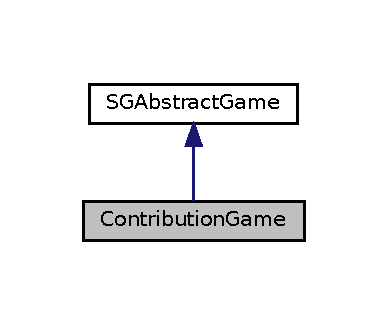
\includegraphics[width=186pt]{classContributionGame__inherit__graph}
\end{center}
\end{figure}


Collaboration diagram for Contribution\+Game\+:
\nopagebreak
\begin{figure}[H]
\begin{center}
\leavevmode
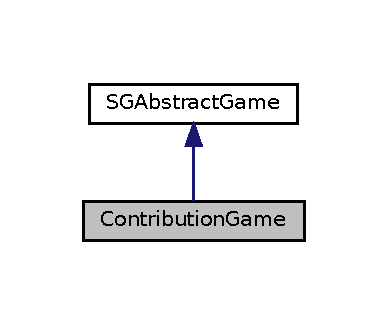
\includegraphics[width=186pt]{classContributionGame__coll__graph}
\end{center}
\end{figure}
\subsection*{Public Member Functions}
\begin{DoxyCompactItemize}
\item 
\mbox{\Hypertarget{classContributionGame_aa642964959782aaed1d86a0d38d32493}\label{classContributionGame_aa642964959782aaed1d86a0d38d32493}} 
{\bfseries Contribution\+Game} (int \+\_\+num\+Players, double \+\_\+delta, int \+\_\+num\+States)
\item 
virtual \hyperlink{classSGPoint}{S\+G\+Point} \hyperlink{classContributionGame_ab33daef685ec7b22c44dad283c2f88cd}{payoffs} (int state, const vector$<$ int $>$ \&actions) const
\begin{DoxyCompactList}\small\item\em The payoff function. \end{DoxyCompactList}\item 
virtual double \hyperlink{classContributionGame_a7b5ca7f6f0119f5899784ceae570666d}{probability} (int state, const vector$<$ int $>$ \&actions, int statep) const
\begin{DoxyCompactList}\small\item\em Transition probabilities. \end{DoxyCompactList}\end{DoxyCompactItemize}
\subsection*{Additional Inherited Members}


\subsection{Detailed Description}
N-\/player prisoners\textquotesingle{} contribution game. 

$<$ This class implements a multi-\/player prisoners\textquotesingle{} dilemma with two states and uniform transition probabilities. 

\subsection{Member Function Documentation}
\mbox{\Hypertarget{classContributionGame_ab33daef685ec7b22c44dad283c2f88cd}\label{classContributionGame_ab33daef685ec7b22c44dad283c2f88cd}} 
\index{Contribution\+Game@{Contribution\+Game}!payoffs@{payoffs}}
\index{payoffs@{payoffs}!Contribution\+Game@{Contribution\+Game}}
\subsubsection{\texorpdfstring{payoffs()}{payoffs()}}
{\footnotesize\ttfamily virtual \hyperlink{classSGPoint}{S\+G\+Point} Contribution\+Game\+::payoffs (\begin{DoxyParamCaption}\item[{int}]{state,  }\item[{const vector$<$ int $>$ \&}]{actions }\end{DoxyParamCaption}) const\hspace{0.3cm}{\ttfamily [inline]}, {\ttfamily [virtual]}}



The payoff function. 

A class that is derived from \hyperlink{classSGAbstractGame}{S\+G\+Abstract\+Game} must define the payoffs method, which returns, for a given state and action pair, the flow payoffs that the players receive as an \hyperlink{classSGPoint}{S\+G\+Point}. 

Implements \hyperlink{classSGAbstractGame_a3fc1cd009d1813f44f1f219e7deb6eef}{S\+G\+Abstract\+Game}.

\mbox{\Hypertarget{classContributionGame_a7b5ca7f6f0119f5899784ceae570666d}\label{classContributionGame_a7b5ca7f6f0119f5899784ceae570666d}} 
\index{Contribution\+Game@{Contribution\+Game}!probability@{probability}}
\index{probability@{probability}!Contribution\+Game@{Contribution\+Game}}
\subsubsection{\texorpdfstring{probability()}{probability()}}
{\footnotesize\ttfamily virtual double Contribution\+Game\+::probability (\begin{DoxyParamCaption}\item[{int}]{state,  }\item[{const vector$<$ int $>$ \&}]{actions,  }\item[{int}]{statep }\end{DoxyParamCaption}) const\hspace{0.3cm}{\ttfamily [inline]}, {\ttfamily [virtual]}}



Transition probabilities. 

A class that derives from \hyperlink{classSGAbstractGame}{S\+G\+Abstract\+Game} must define the probability method, which gives, for each state and action pair and new state, the probability of reaching the new state tomorrow when starting from the given state and when the given action pair is played. 

Implements \hyperlink{classSGAbstractGame_a416b31d5020b75de49447ce4f7783b98}{S\+G\+Abstract\+Game}.



The documentation for this class was generated from the following file\+:\begin{DoxyCompactItemize}
\item 
src/hpp/sgcontribution.\+hpp\end{DoxyCompactItemize}

\hypertarget{classstd_1_1list_3_01SGAction_01_4}{}\section{std\+:\+:list$<$ S\+G\+Action $>$ Class Reference}
\label{classstd_1_1list_3_01SGAction_01_4}\index{std\+::list$<$ S\+G\+Action $>$@{std\+::list$<$ S\+G\+Action $>$}}


Collaboration diagram for std\+:\+:list$<$ S\+G\+Action $>$\+:
\nopagebreak
\begin{figure}[H]
\begin{center}
\leavevmode
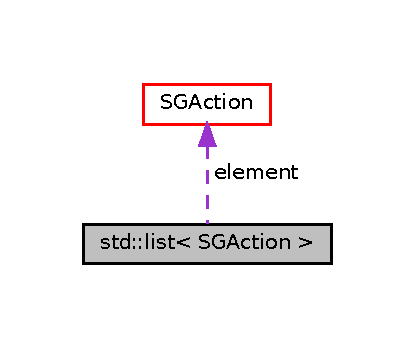
\includegraphics[width=199pt]{classstd_1_1list_3_01SGAction_01_4__coll__graph}
\end{center}
\end{figure}
\subsection*{Public Attributes}
\begin{DoxyCompactItemize}
\item 
\mbox{\Hypertarget{classstd_1_1list_3_01SGAction_01_4_ab9a0b8b7942980ededf0f2440901fb67}\label{classstd_1_1list_3_01SGAction_01_4_ab9a0b8b7942980ededf0f2440901fb67}} 
\hyperlink{classSGAction}{S\+G\+Action} {\bfseries element}
\end{DoxyCompactItemize}


The documentation for this class was generated from the following file\+:\begin{DoxyCompactItemize}
\item 
src/hpp/sgstl.\+cpp\end{DoxyCompactItemize}

\hypertarget{classstd_1_1list_3_01SGIteration_01_4}{}\section{std\+:\+:list$<$ S\+G\+Iteration $>$ Class Reference}
\label{classstd_1_1list_3_01SGIteration_01_4}\index{std\+::list$<$ S\+G\+Iteration $>$@{std\+::list$<$ S\+G\+Iteration $>$}}


Collaboration diagram for std\+:\+:list$<$ S\+G\+Iteration $>$\+:
\nopagebreak
\begin{figure}[H]
\begin{center}
\leavevmode
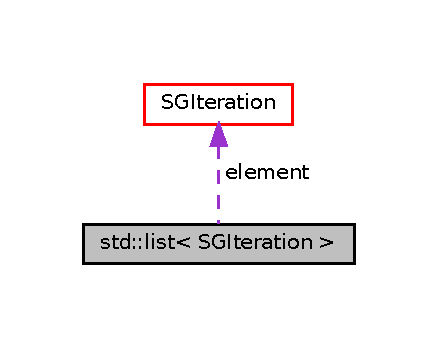
\includegraphics[width=210pt]{classstd_1_1list_3_01SGIteration_01_4__coll__graph}
\end{center}
\end{figure}
\subsection*{Public Attributes}
\begin{DoxyCompactItemize}
\item 
\mbox{\Hypertarget{classstd_1_1list_3_01SGIteration_01_4_a3ae13353092ca4ddc13181f31e4193fe}\label{classstd_1_1list_3_01SGIteration_01_4_a3ae13353092ca4ddc13181f31e4193fe}} 
\hyperlink{classSGIteration}{S\+G\+Iteration} {\bfseries element}
\end{DoxyCompactItemize}


The documentation for this class was generated from the following file\+:\begin{DoxyCompactItemize}
\item 
src/hpp/sgstl.\+cpp\end{DoxyCompactItemize}

\hypertarget{classstd_1_1list_3_01SGIteration__MaxMinMax_01_4}{}\section{std\+:\+:list$<$ S\+G\+Iteration\+\_\+\+Max\+Min\+Max $>$ Class Reference}
\label{classstd_1_1list_3_01SGIteration__MaxMinMax_01_4}\index{std\+::list$<$ S\+G\+Iteration\+\_\+\+Max\+Min\+Max $>$@{std\+::list$<$ S\+G\+Iteration\+\_\+\+Max\+Min\+Max $>$}}


Collaboration diagram for std\+:\+:list$<$ S\+G\+Iteration\+\_\+\+Max\+Min\+Max $>$\+:
\nopagebreak
\begin{figure}[H]
\begin{center}
\leavevmode
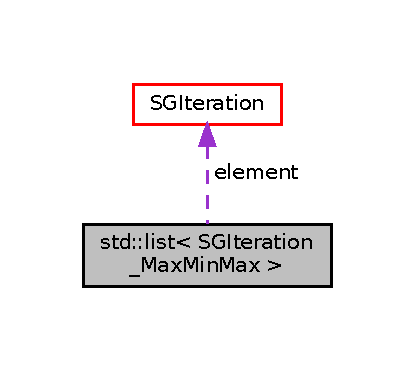
\includegraphics[width=199pt]{classstd_1_1list_3_01SGIteration__MaxMinMax_01_4__coll__graph}
\end{center}
\end{figure}
\subsection*{Public Attributes}
\begin{DoxyCompactItemize}
\item 
\mbox{\Hypertarget{classstd_1_1list_3_01SGIteration__MaxMinMax_01_4_a1aa648739f53cf8bc81864aededf7ad3}\label{classstd_1_1list_3_01SGIteration__MaxMinMax_01_4_a1aa648739f53cf8bc81864aededf7ad3}} 
\hyperlink{classSGIteration}{S\+G\+Iteration} {\bfseries element}
\end{DoxyCompactItemize}


The documentation for this class was generated from the following file\+:\begin{DoxyCompactItemize}
\item 
src/hpp/sgstl.\+cpp\end{DoxyCompactItemize}

\hypertarget{classstd_1_1list_3_01SGStep_01_4}{}\section{std\+:\+:list$<$ S\+G\+Step $>$ Class Reference}
\label{classstd_1_1list_3_01SGStep_01_4}\index{std\+::list$<$ S\+G\+Step $>$@{std\+::list$<$ S\+G\+Step $>$}}


Collaboration diagram for std\+:\+:list$<$ S\+G\+Step $>$\+:
\nopagebreak
\begin{figure}[H]
\begin{center}
\leavevmode
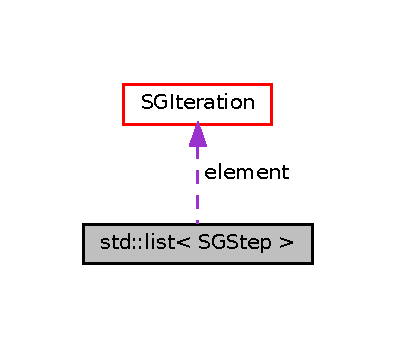
\includegraphics[width=190pt]{classstd_1_1list_3_01SGStep_01_4__coll__graph}
\end{center}
\end{figure}
\subsection*{Public Attributes}
\begin{DoxyCompactItemize}
\item 
\mbox{\Hypertarget{classstd_1_1list_3_01SGStep_01_4_a918e6d638b82e9344f4aa20c83ff8f7a}\label{classstd_1_1list_3_01SGStep_01_4_a918e6d638b82e9344f4aa20c83ff8f7a}} 
\hyperlink{classSGIteration}{S\+G\+Iteration} {\bfseries element}
\end{DoxyCompactItemize}


The documentation for this class was generated from the following file\+:\begin{DoxyCompactItemize}
\item 
src/hpp/sgstl.\+cpp\end{DoxyCompactItemize}

\hypertarget{classstd_1_1list_3_01SGTuple_01_4}{}\section{std\+:\+:list$<$ S\+G\+Tuple $>$ Class Reference}
\label{classstd_1_1list_3_01SGTuple_01_4}\index{std\+::list$<$ S\+G\+Tuple $>$@{std\+::list$<$ S\+G\+Tuple $>$}}


Collaboration diagram for std\+:\+:list$<$ S\+G\+Tuple $>$\+:
\nopagebreak
\begin{figure}[H]
\begin{center}
\leavevmode
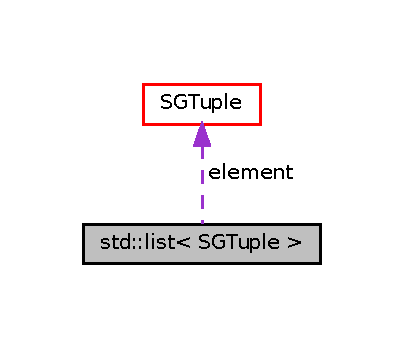
\includegraphics[width=194pt]{classstd_1_1list_3_01SGTuple_01_4__coll__graph}
\end{center}
\end{figure}
\subsection*{Public Attributes}
\begin{DoxyCompactItemize}
\item 
\mbox{\Hypertarget{classstd_1_1list_3_01SGTuple_01_4_ac4c14c4d995b52e5d3b08fd07b38f0af}\label{classstd_1_1list_3_01SGTuple_01_4_ac4c14c4d995b52e5d3b08fd07b38f0af}} 
\hyperlink{classSGTuple}{S\+G\+Tuple} {\bfseries element}
\end{DoxyCompactItemize}


The documentation for this class was generated from the following file\+:\begin{DoxyCompactItemize}
\item 
src/hpp/sgstl.\+cpp\end{DoxyCompactItemize}

\hypertarget{structpolicyComp}{}\section{policy\+Comp Struct Reference}
\label{structpolicyComp}\index{policy\+Comp@{policy\+Comp}}


Function object for comparing two policies.  




{\ttfamily \#include $<$sgproductpolicy.\+hpp$>$}

\subsection*{Public Member Functions}
\begin{DoxyCompactItemize}
\item 
\mbox{\Hypertarget{structpolicyComp_ab3833f236dea57a4ee36cce768d6869e}\label{structpolicyComp_ab3833f236dea57a4ee36cce768d6869e}} 
bool {\bfseries operator()} (const \hyperlink{classSGPolicy}{S\+G\+Policy} \&lhs, const \hyperlink{classSGPolicy}{S\+G\+Policy} \&rhs)
\end{DoxyCompactItemize}


\subsection{Detailed Description}
Function object for comparing two policies. 

The documentation for this struct was generated from the following file\+:\begin{DoxyCompactItemize}
\item 
src/hpp/sgproductpolicy.\+hpp\end{DoxyCompactItemize}

\hypertarget{classRiskSharingGame}{}\section{Risk\+Sharing\+Game Class Reference}
\label{classRiskSharingGame}\index{Risk\+Sharing\+Game@{Risk\+Sharing\+Game}}


Two player version of the Kocherlakota (1996) risk sharing game.  




{\ttfamily \#include $<$sgrisksharing.\+hpp$>$}



Inheritance diagram for Risk\+Sharing\+Game\+:
\nopagebreak
\begin{figure}[H]
\begin{center}
\leavevmode
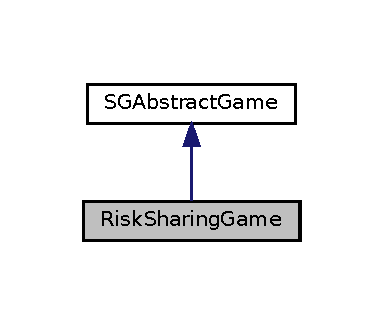
\includegraphics[width=184pt]{classRiskSharingGame__inherit__graph}
\end{center}
\end{figure}


Collaboration diagram for Risk\+Sharing\+Game\+:
\nopagebreak
\begin{figure}[H]
\begin{center}
\leavevmode
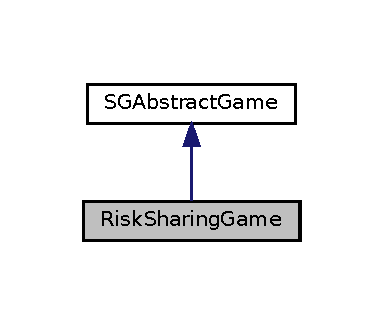
\includegraphics[width=184pt]{classRiskSharingGame__coll__graph}
\end{center}
\end{figure}
\subsection*{Public Types}
\begin{DoxyCompactItemize}
\item 
\mbox{\Hypertarget{classRiskSharingGame_a5645d88336b8df49bf98e6e2d109f4cf}\label{classRiskSharingGame_a5645d88336b8df49bf98e6e2d109f4cf}} 
enum {\bfseries Endowment\+Mode} \{ {\bfseries Consumption}, 
{\bfseries Endowment}
 \}
\end{DoxyCompactItemize}
\subsection*{Public Member Functions}
\begin{DoxyCompactItemize}
\item 
\mbox{\Hypertarget{classRiskSharingGame_a45791290b135201e5ef5e5785c967748}\label{classRiskSharingGame_a45791290b135201e5ef5e5785c967748}} 
{\bfseries Risk\+Sharing\+Game} (double \hyperlink{classSGAbstractGame_a34c8905ac463bb2ec54aba4eb4ac376f}{delta}, int \+\_\+num\+Endowments, int \+\_\+c2e, double \+\_\+persistence, Endowment\+Mode \+\_\+mode)
\item 
virtual \hyperlink{classSGPoint}{S\+G\+Point} \hyperlink{classRiskSharingGame_a2aed9769b6518ed68b0c595629fb0129}{payoffs} (int state, const vector$<$ int $>$ \&actions) const
\begin{DoxyCompactList}\small\item\em The payoff function. \end{DoxyCompactList}\item 
virtual double \hyperlink{classRiskSharingGame_aa9ae41ec3aec3342ffd2d16187746718}{probability} (int e, const vector$<$ int $>$ \&actions, int ep) const
\begin{DoxyCompactList}\small\item\em Transition probabilities. \end{DoxyCompactList}\item 
virtual bool \hyperlink{classRiskSharingGame_a7da6b669317562cd9df8dfc0f8226b4c}{is\+Equilibrium\+Action} (int state, const vector$<$ int $>$ \&actions) const
\end{DoxyCompactItemize}
\subsection*{Private Member Functions}
\begin{DoxyCompactItemize}
\item 
\mbox{\Hypertarget{classRiskSharingGame_afc7b13c5ac6db8692cc4fb7760cee8dd}\label{classRiskSharingGame_afc7b13c5ac6db8692cc4fb7760cee8dd}} 
double {\bfseries consumption} (int e, int t) const
\item 
\mbox{\Hypertarget{classRiskSharingGame_a8d6ce5f102ec1b4b87a8c4ea0e904c1c}\label{classRiskSharingGame_a8d6ce5f102ec1b4b87a8c4ea0e904c1c}} 
double {\bfseries cdf} (double x) const
\item 
\mbox{\Hypertarget{classRiskSharingGame_aef9d8593ca6d1666a712b23d7cedede7}\label{classRiskSharingGame_aef9d8593ca6d1666a712b23d7cedede7}} 
double {\bfseries prob\+Helper} (int e, int t, int ep) const
\end{DoxyCompactItemize}
\subsection*{Private Attributes}
\begin{DoxyCompactItemize}
\item 
\mbox{\Hypertarget{classRiskSharingGame_a8236f900f444fa81985d42364f5052d5}\label{classRiskSharingGame_a8236f900f444fa81985d42364f5052d5}} 
int {\bfseries num\+Endowments}
\item 
\mbox{\Hypertarget{classRiskSharingGame_abbc092fe82572dd91278124713ecdce6}\label{classRiskSharingGame_abbc092fe82572dd91278124713ecdce6}} 
int {\bfseries c2e}
\item 
\mbox{\Hypertarget{classRiskSharingGame_a0bb2edd8646a536d2e70b960c2a27ffa}\label{classRiskSharingGame_a0bb2edd8646a536d2e70b960c2a27ffa}} 
double {\bfseries persistence}
\item 
\mbox{\Hypertarget{classRiskSharingGame_a2aefe50f2cac37e7226f490303f6ecdb}\label{classRiskSharingGame_a2aefe50f2cac37e7226f490303f6ecdb}} 
vector$<$ double $>$ {\bfseries E}
\item 
\mbox{\Hypertarget{classRiskSharingGame_a667851c4a7814e141164953615253960}\label{classRiskSharingGame_a667851c4a7814e141164953615253960}} 
int {\bfseries mid\+Point}
\item 
\mbox{\Hypertarget{classRiskSharingGame_a2461185db47c09248dff9ba24096aa04}\label{classRiskSharingGame_a2461185db47c09248dff9ba24096aa04}} 
double {\bfseries e\+Incr}
\item 
\mbox{\Hypertarget{classRiskSharingGame_a494738415dfc21e87c7de3e79c0ab852}\label{classRiskSharingGame_a494738415dfc21e87c7de3e79c0ab852}} 
double {\bfseries c\+Incr}
\item 
\mbox{\Hypertarget{classRiskSharingGame_a710c6947fefecf2d3018c4bc07a50cf6}\label{classRiskSharingGame_a710c6947fefecf2d3018c4bc07a50cf6}} 
vector$<$ vector$<$ double $>$ $>$ {\bfseries state\+Prob\+Sum}
\item 
\mbox{\Hypertarget{classRiskSharingGame_a8891d49871f4f19cab0fc2e7beb14345}\label{classRiskSharingGame_a8891d49871f4f19cab0fc2e7beb14345}} 
vector$<$ int $>$ {\bfseries num\+Actions\+\_\+total}
\item 
\mbox{\Hypertarget{classRiskSharingGame_a82b03b56b74462d424fd7dedf8870dc9}\label{classRiskSharingGame_a82b03b56b74462d424fd7dedf8870dc9}} 
Endowment\+Mode {\bfseries endowment\+Mode}
\end{DoxyCompactItemize}
\subsection*{Additional Inherited Members}


\subsection{Detailed Description}
Two player version of the Kocherlakota (1996) risk sharing game. \begin{Desc}
\item[Examples\+: ]\par
\hyperlink{risksharing_maxminmax_8cpp-example}{risksharing\+\_\+maxminmax.\+cpp}.\end{Desc}


\subsection{Member Function Documentation}
\mbox{\Hypertarget{classRiskSharingGame_a7da6b669317562cd9df8dfc0f8226b4c}\label{classRiskSharingGame_a7da6b669317562cd9df8dfc0f8226b4c}} 
\index{Risk\+Sharing\+Game@{Risk\+Sharing\+Game}!is\+Equilibrium\+Action@{is\+Equilibrium\+Action}}
\index{is\+Equilibrium\+Action@{is\+Equilibrium\+Action}!Risk\+Sharing\+Game@{Risk\+Sharing\+Game}}
\subsubsection{\texorpdfstring{is\+Equilibrium\+Action()}{isEquilibriumAction()}}
{\footnotesize\ttfamily virtual bool Risk\+Sharing\+Game\+::is\+Equilibrium\+Action (\begin{DoxyParamCaption}\item[{int}]{state,  }\item[{const vector$<$ int $>$ \&}]{actions }\end{DoxyParamCaption}) const\hspace{0.3cm}{\ttfamily [inline]}, {\ttfamily [virtual]}}

Returns true if the given action pair can be played in equilibrium

The default definition of this method always returns true, so that all action pairs can be played in equilibrium. By redefining this method, the user can create models in which only a subset of action pairs are played on the equilibrium path. 

Reimplemented from \hyperlink{classSGAbstractGame_a2cec8147c3055cfe6314da349d1a7344}{S\+G\+Abstract\+Game}.

\mbox{\Hypertarget{classRiskSharingGame_a2aed9769b6518ed68b0c595629fb0129}\label{classRiskSharingGame_a2aed9769b6518ed68b0c595629fb0129}} 
\index{Risk\+Sharing\+Game@{Risk\+Sharing\+Game}!payoffs@{payoffs}}
\index{payoffs@{payoffs}!Risk\+Sharing\+Game@{Risk\+Sharing\+Game}}
\subsubsection{\texorpdfstring{payoffs()}{payoffs()}}
{\footnotesize\ttfamily virtual \hyperlink{classSGPoint}{S\+G\+Point} Risk\+Sharing\+Game\+::payoffs (\begin{DoxyParamCaption}\item[{int}]{state,  }\item[{const vector$<$ int $>$ \&}]{actions }\end{DoxyParamCaption}) const\hspace{0.3cm}{\ttfamily [inline]}, {\ttfamily [virtual]}}



The payoff function. 

A class that is derived from \hyperlink{classSGAbstractGame}{S\+G\+Abstract\+Game} must define the payoffs method, which returns, for a given state and action pair, the flow payoffs that the players receive as an \hyperlink{classSGPoint}{S\+G\+Point}. 

Implements \hyperlink{classSGAbstractGame_a3fc1cd009d1813f44f1f219e7deb6eef}{S\+G\+Abstract\+Game}.

\mbox{\Hypertarget{classRiskSharingGame_aa9ae41ec3aec3342ffd2d16187746718}\label{classRiskSharingGame_aa9ae41ec3aec3342ffd2d16187746718}} 
\index{Risk\+Sharing\+Game@{Risk\+Sharing\+Game}!probability@{probability}}
\index{probability@{probability}!Risk\+Sharing\+Game@{Risk\+Sharing\+Game}}
\subsubsection{\texorpdfstring{probability()}{probability()}}
{\footnotesize\ttfamily virtual double Risk\+Sharing\+Game\+::probability (\begin{DoxyParamCaption}\item[{int}]{state,  }\item[{const vector$<$ int $>$ \&}]{actions,  }\item[{int}]{statep }\end{DoxyParamCaption}) const\hspace{0.3cm}{\ttfamily [inline]}, {\ttfamily [virtual]}}



Transition probabilities. 

A class that derives from \hyperlink{classSGAbstractGame}{S\+G\+Abstract\+Game} must define the probability method, which gives, for each state and action pair and new state, the probability of reaching the new state tomorrow when starting from the given state and when the given action pair is played. 

Implements \hyperlink{classSGAbstractGame_a416b31d5020b75de49447ce4f7783b98}{S\+G\+Abstract\+Game}.



The documentation for this class was generated from the following file\+:\begin{DoxyCompactItemize}
\item 
src/hpp/sgrisksharing.\+hpp\end{DoxyCompactItemize}

\hypertarget{classRiskSharingGame__3Player}{}\section{Risk\+Sharing\+Game\+\_\+3\+Player Class Reference}
\label{classRiskSharingGame__3Player}\index{Risk\+Sharing\+Game\+\_\+3\+Player@{Risk\+Sharing\+Game\+\_\+3\+Player}}


Three player version of the Kocherlakota (1996) risk sharing game.  




{\ttfamily \#include $<$sgrisksharing\+\_\+3player.\+hpp$>$}



Inheritance diagram for Risk\+Sharing\+Game\+\_\+3\+Player\+:
\nopagebreak
\begin{figure}[H]
\begin{center}
\leavevmode
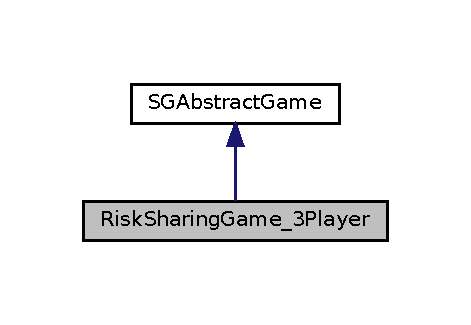
\includegraphics[width=226pt]{classRiskSharingGame__3Player__inherit__graph}
\end{center}
\end{figure}


Collaboration diagram for Risk\+Sharing\+Game\+\_\+3\+Player\+:
\nopagebreak
\begin{figure}[H]
\begin{center}
\leavevmode
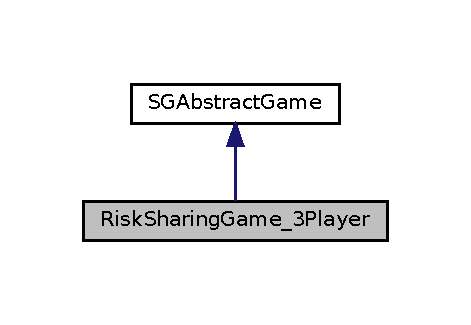
\includegraphics[width=226pt]{classRiskSharingGame__3Player__coll__graph}
\end{center}
\end{figure}
\subsection*{Public Member Functions}
\begin{DoxyCompactItemize}
\item 
\mbox{\Hypertarget{classRiskSharingGame__3Player_aa04f71baa89e13f2411c27ec51d5ad44}\label{classRiskSharingGame__3Player_aa04f71baa89e13f2411c27ec51d5ad44}} 
{\bfseries Risk\+Sharing\+Game\+\_\+3\+Player} (double \hyperlink{classSGAbstractGame_a34c8905ac463bb2ec54aba4eb4ac376f}{delta}, int \+\_\+num\+Endowments, int \+\_\+c2e)
\item 
virtual \hyperlink{classSGPoint}{S\+G\+Point} \hyperlink{classRiskSharingGame__3Player_ae4a07f7dc66f18eccd29bc7993c0472f}{payoffs} (int state, const vector$<$ int $>$ \&actions) const
\begin{DoxyCompactList}\small\item\em The payoff function. \end{DoxyCompactList}\item 
virtual double \hyperlink{classRiskSharingGame__3Player_a48f478394bae9cf7479519da9b18a987}{probability} (int e, const vector$<$ int $>$ \&actions, int ep) const
\begin{DoxyCompactList}\small\item\em Transition probabilities. \end{DoxyCompactList}\item 
virtual bool \hyperlink{classRiskSharingGame__3Player_a79f44b04c558ecd72cf0b464fdd8a317}{is\+Equilibrium\+Action} (int state, const vector$<$ int $>$ \&actions) const
\end{DoxyCompactItemize}
\subsection*{Private Attributes}
\begin{DoxyCompactItemize}
\item 
\mbox{\Hypertarget{classRiskSharingGame__3Player_ab3687b044f23019a5c66b05675ecd963}\label{classRiskSharingGame__3Player_ab3687b044f23019a5c66b05675ecd963}} 
int {\bfseries num\+Endowments}
\item 
\mbox{\Hypertarget{classRiskSharingGame__3Player_a3572e0f51a0cd11fbc34db0f6d323ab5}\label{classRiskSharingGame__3Player_a3572e0f51a0cd11fbc34db0f6d323ab5}} 
int {\bfseries c2e}
\item 
\mbox{\Hypertarget{classRiskSharingGame__3Player_a8ea60c87e78bbcafaf3dbbd8fd7b5712}\label{classRiskSharingGame__3Player_a8ea60c87e78bbcafaf3dbbd8fd7b5712}} 
vector$<$ vector$<$ int $>$ $>$ {\bfseries E}
\item 
\mbox{\Hypertarget{classRiskSharingGame__3Player_a27081a99338c5dc81faa8ca74d15ba32}\label{classRiskSharingGame__3Player_a27081a99338c5dc81faa8ca74d15ba32}} 
double {\bfseries e\+Incr}
\item 
\mbox{\Hypertarget{classRiskSharingGame__3Player_a2615654d1b8aee618d9f8c1e99e56c33}\label{classRiskSharingGame__3Player_a2615654d1b8aee618d9f8c1e99e56c33}} 
double {\bfseries c\+Incr}
\item 
\mbox{\Hypertarget{classRiskSharingGame__3Player_a11819cbe897fd8246c70ae2295a32e6a}\label{classRiskSharingGame__3Player_a11819cbe897fd8246c70ae2295a32e6a}} 
vector$<$ int $>$ {\bfseries num\+Actions\+\_\+total}
\item 
\mbox{\Hypertarget{classRiskSharingGame__3Player_ab42d33f21d8b835aacdc9f2d3813bad0}\label{classRiskSharingGame__3Player_ab42d33f21d8b835aacdc9f2d3813bad0}} 
vector$<$ vector$<$ int $>$ $>$ {\bfseries transfer\+List}
\end{DoxyCompactItemize}
\subsection*{Additional Inherited Members}


\subsection{Detailed Description}
Three player version of the Kocherlakota (1996) risk sharing game. 

\subsection{Member Function Documentation}
\mbox{\Hypertarget{classRiskSharingGame__3Player_a79f44b04c558ecd72cf0b464fdd8a317}\label{classRiskSharingGame__3Player_a79f44b04c558ecd72cf0b464fdd8a317}} 
\index{Risk\+Sharing\+Game\+\_\+3\+Player@{Risk\+Sharing\+Game\+\_\+3\+Player}!is\+Equilibrium\+Action@{is\+Equilibrium\+Action}}
\index{is\+Equilibrium\+Action@{is\+Equilibrium\+Action}!Risk\+Sharing\+Game\+\_\+3\+Player@{Risk\+Sharing\+Game\+\_\+3\+Player}}
\subsubsection{\texorpdfstring{is\+Equilibrium\+Action()}{isEquilibriumAction()}}
{\footnotesize\ttfamily virtual bool Risk\+Sharing\+Game\+\_\+3\+Player\+::is\+Equilibrium\+Action (\begin{DoxyParamCaption}\item[{int}]{state,  }\item[{const vector$<$ int $>$ \&}]{actions }\end{DoxyParamCaption}) const\hspace{0.3cm}{\ttfamily [inline]}, {\ttfamily [virtual]}}

Returns true if the given action pair can be played in equilibrium

The default definition of this method always returns true, so that all action pairs can be played in equilibrium. By redefining this method, the user can create models in which only a subset of action pairs are played on the equilibrium path. 

Reimplemented from \hyperlink{classSGAbstractGame_a2cec8147c3055cfe6314da349d1a7344}{S\+G\+Abstract\+Game}.

\mbox{\Hypertarget{classRiskSharingGame__3Player_ae4a07f7dc66f18eccd29bc7993c0472f}\label{classRiskSharingGame__3Player_ae4a07f7dc66f18eccd29bc7993c0472f}} 
\index{Risk\+Sharing\+Game\+\_\+3\+Player@{Risk\+Sharing\+Game\+\_\+3\+Player}!payoffs@{payoffs}}
\index{payoffs@{payoffs}!Risk\+Sharing\+Game\+\_\+3\+Player@{Risk\+Sharing\+Game\+\_\+3\+Player}}
\subsubsection{\texorpdfstring{payoffs()}{payoffs()}}
{\footnotesize\ttfamily virtual \hyperlink{classSGPoint}{S\+G\+Point} Risk\+Sharing\+Game\+\_\+3\+Player\+::payoffs (\begin{DoxyParamCaption}\item[{int}]{state,  }\item[{const vector$<$ int $>$ \&}]{actions }\end{DoxyParamCaption}) const\hspace{0.3cm}{\ttfamily [inline]}, {\ttfamily [virtual]}}



The payoff function. 

A class that is derived from \hyperlink{classSGAbstractGame}{S\+G\+Abstract\+Game} must define the payoffs method, which returns, for a given state and action pair, the flow payoffs that the players receive as an \hyperlink{classSGPoint}{S\+G\+Point}. 

Implements \hyperlink{classSGAbstractGame_a3fc1cd009d1813f44f1f219e7deb6eef}{S\+G\+Abstract\+Game}.

\mbox{\Hypertarget{classRiskSharingGame__3Player_a48f478394bae9cf7479519da9b18a987}\label{classRiskSharingGame__3Player_a48f478394bae9cf7479519da9b18a987}} 
\index{Risk\+Sharing\+Game\+\_\+3\+Player@{Risk\+Sharing\+Game\+\_\+3\+Player}!probability@{probability}}
\index{probability@{probability}!Risk\+Sharing\+Game\+\_\+3\+Player@{Risk\+Sharing\+Game\+\_\+3\+Player}}
\subsubsection{\texorpdfstring{probability()}{probability()}}
{\footnotesize\ttfamily virtual double Risk\+Sharing\+Game\+\_\+3\+Player\+::probability (\begin{DoxyParamCaption}\item[{int}]{state,  }\item[{const vector$<$ int $>$ \&}]{actions,  }\item[{int}]{statep }\end{DoxyParamCaption}) const\hspace{0.3cm}{\ttfamily [inline]}, {\ttfamily [virtual]}}



Transition probabilities. 

A class that derives from \hyperlink{classSGAbstractGame}{S\+G\+Abstract\+Game} must define the probability method, which gives, for each state and action pair and new state, the probability of reaching the new state tomorrow when starting from the given state and when the given action pair is played. 

Implements \hyperlink{classSGAbstractGame_a416b31d5020b75de49447ce4f7783b98}{S\+G\+Abstract\+Game}.



The documentation for this class was generated from the following file\+:\begin{DoxyCompactItemize}
\item 
src/hpp/sgrisksharing\+\_\+3player.\+hpp\end{DoxyCompactItemize}

\hypertarget{classRiskSharingGame__3Player__Merged}{}\section{Risk\+Sharing\+Game\+\_\+3\+Player\+\_\+\+Merged Class Reference}
\label{classRiskSharingGame__3Player__Merged}\index{Risk\+Sharing\+Game\+\_\+3\+Player\+\_\+\+Merged@{Risk\+Sharing\+Game\+\_\+3\+Player\+\_\+\+Merged}}


Two player version of the Kocherlakota (1996) risk sharing game.  




{\ttfamily \#include $<$sgrisksharing\+\_\+3player\+\_\+merged.\+hpp$>$}



Inheritance diagram for Risk\+Sharing\+Game\+\_\+3\+Player\+\_\+\+Merged\+:
\nopagebreak
\begin{figure}[H]
\begin{center}
\leavevmode
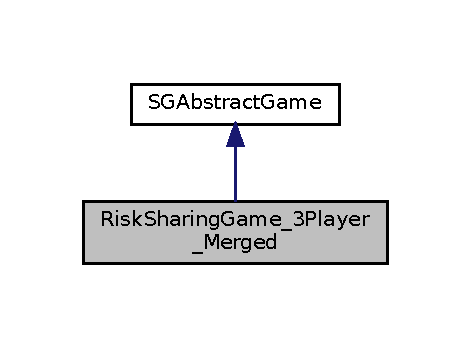
\includegraphics[width=226pt]{classRiskSharingGame__3Player__Merged__inherit__graph}
\end{center}
\end{figure}


Collaboration diagram for Risk\+Sharing\+Game\+\_\+3\+Player\+\_\+\+Merged\+:
\nopagebreak
\begin{figure}[H]
\begin{center}
\leavevmode
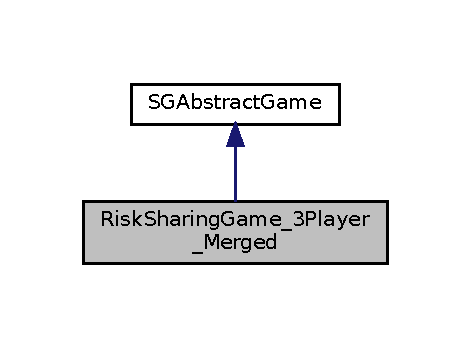
\includegraphics[width=226pt]{classRiskSharingGame__3Player__Merged__coll__graph}
\end{center}
\end{figure}
\subsection*{Public Member Functions}
\begin{DoxyCompactItemize}
\item 
\mbox{\Hypertarget{classRiskSharingGame__3Player__Merged_a32094245f4ee1427cb306705b03249d9}\label{classRiskSharingGame__3Player__Merged_a32094245f4ee1427cb306705b03249d9}} 
{\bfseries Risk\+Sharing\+Game\+\_\+3\+Player\+\_\+\+Merged} (double \hyperlink{classSGAbstractGame_a34c8905ac463bb2ec54aba4eb4ac376f}{delta}, int \+\_\+num\+Endowments, int \+\_\+c2e)
\item 
virtual \hyperlink{classSGPoint}{S\+G\+Point} \hyperlink{classRiskSharingGame__3Player__Merged_aa1d807770ff356fe1114d17966172fbd}{payoffs} (int state, const vector$<$ int $>$ \&actions) const
\begin{DoxyCompactList}\small\item\em The payoff function. \end{DoxyCompactList}\item 
virtual double \hyperlink{classRiskSharingGame__3Player__Merged_a505d06e31a1cabde1c6fab8ac5af8409}{probability} (int e, const vector$<$ int $>$ \&actions, int ep) const
\begin{DoxyCompactList}\small\item\em Transition probabilities. \end{DoxyCompactList}\item 
virtual bool \hyperlink{classRiskSharingGame__3Player__Merged_aeff4f08e00ef46bbdbb190c9c6c393a4}{is\+Equilibrium\+Action} (int state, const vector$<$ int $>$ \&actions) const
\end{DoxyCompactItemize}
\subsection*{Private Member Functions}
\begin{DoxyCompactItemize}
\item 
\mbox{\Hypertarget{classRiskSharingGame__3Player__Merged_a9d26ce7c0e2d6734f6501ae82d173e96}\label{classRiskSharingGame__3Player__Merged_a9d26ce7c0e2d6734f6501ae82d173e96}} 
double {\bfseries consumption} (int e, int t) const
\end{DoxyCompactItemize}
\subsection*{Private Attributes}
\begin{DoxyCompactItemize}
\item 
\mbox{\Hypertarget{classRiskSharingGame__3Player__Merged_a99abe786dd53923789d99e86791affd3}\label{classRiskSharingGame__3Player__Merged_a99abe786dd53923789d99e86791affd3}} 
int {\bfseries num\+Endowments}
\item 
\mbox{\Hypertarget{classRiskSharingGame__3Player__Merged_a6e775a19ff8f5141b2e7b8575885401d}\label{classRiskSharingGame__3Player__Merged_a6e775a19ff8f5141b2e7b8575885401d}} 
int {\bfseries c2e}
\item 
\mbox{\Hypertarget{classRiskSharingGame__3Player__Merged_acb4be7edf1f8e280748b8c1bd6992a10}\label{classRiskSharingGame__3Player__Merged_acb4be7edf1f8e280748b8c1bd6992a10}} 
vector$<$ double $>$ {\bfseries E}
\item 
\mbox{\Hypertarget{classRiskSharingGame__3Player__Merged_a0f2acb80b7834d796c61fb956934a91f}\label{classRiskSharingGame__3Player__Merged_a0f2acb80b7834d796c61fb956934a91f}} 
double {\bfseries e\+Incr}
\item 
\mbox{\Hypertarget{classRiskSharingGame__3Player__Merged_a711d6e50ccd05e36c01f961d2690abae}\label{classRiskSharingGame__3Player__Merged_a711d6e50ccd05e36c01f961d2690abae}} 
double {\bfseries c\+Incr}
\item 
\mbox{\Hypertarget{classRiskSharingGame__3Player__Merged_a98326dd60feff58d3fd575c96f99600d}\label{classRiskSharingGame__3Player__Merged_a98326dd60feff58d3fd575c96f99600d}} 
vector$<$ int $>$ {\bfseries num\+Actions\+\_\+total}
\item 
\mbox{\Hypertarget{classRiskSharingGame__3Player__Merged_a979d06cb01dbb5a1babe63220961bf27}\label{classRiskSharingGame__3Player__Merged_a979d06cb01dbb5a1babe63220961bf27}} 
double {\bfseries prob\+Denom}
\end{DoxyCompactItemize}
\subsection*{Additional Inherited Members}


\subsection{Detailed Description}
Two player version of the Kocherlakota (1996) risk sharing game. 

$<$ This version of the game corresponds to the game in \hyperlink{classRiskSharingGame__3Player}{Risk\+Sharing\+Game\+\_\+3\+Player}, but where players 2 and 3 behave cooperatively. 

\subsection{Member Function Documentation}
\mbox{\Hypertarget{classRiskSharingGame__3Player__Merged_aeff4f08e00ef46bbdbb190c9c6c393a4}\label{classRiskSharingGame__3Player__Merged_aeff4f08e00ef46bbdbb190c9c6c393a4}} 
\index{Risk\+Sharing\+Game\+\_\+3\+Player\+\_\+\+Merged@{Risk\+Sharing\+Game\+\_\+3\+Player\+\_\+\+Merged}!is\+Equilibrium\+Action@{is\+Equilibrium\+Action}}
\index{is\+Equilibrium\+Action@{is\+Equilibrium\+Action}!Risk\+Sharing\+Game\+\_\+3\+Player\+\_\+\+Merged@{Risk\+Sharing\+Game\+\_\+3\+Player\+\_\+\+Merged}}
\subsubsection{\texorpdfstring{is\+Equilibrium\+Action()}{isEquilibriumAction()}}
{\footnotesize\ttfamily virtual bool Risk\+Sharing\+Game\+\_\+3\+Player\+\_\+\+Merged\+::is\+Equilibrium\+Action (\begin{DoxyParamCaption}\item[{int}]{state,  }\item[{const vector$<$ int $>$ \&}]{actions }\end{DoxyParamCaption}) const\hspace{0.3cm}{\ttfamily [inline]}, {\ttfamily [virtual]}}

Returns true if the given action pair can be played in equilibrium

The default definition of this method always returns true, so that all action pairs can be played in equilibrium. By redefining this method, the user can create models in which only a subset of action pairs are played on the equilibrium path. 

Reimplemented from \hyperlink{classSGAbstractGame_a2cec8147c3055cfe6314da349d1a7344}{S\+G\+Abstract\+Game}.

\mbox{\Hypertarget{classRiskSharingGame__3Player__Merged_aa1d807770ff356fe1114d17966172fbd}\label{classRiskSharingGame__3Player__Merged_aa1d807770ff356fe1114d17966172fbd}} 
\index{Risk\+Sharing\+Game\+\_\+3\+Player\+\_\+\+Merged@{Risk\+Sharing\+Game\+\_\+3\+Player\+\_\+\+Merged}!payoffs@{payoffs}}
\index{payoffs@{payoffs}!Risk\+Sharing\+Game\+\_\+3\+Player\+\_\+\+Merged@{Risk\+Sharing\+Game\+\_\+3\+Player\+\_\+\+Merged}}
\subsubsection{\texorpdfstring{payoffs()}{payoffs()}}
{\footnotesize\ttfamily virtual \hyperlink{classSGPoint}{S\+G\+Point} Risk\+Sharing\+Game\+\_\+3\+Player\+\_\+\+Merged\+::payoffs (\begin{DoxyParamCaption}\item[{int}]{state,  }\item[{const vector$<$ int $>$ \&}]{actions }\end{DoxyParamCaption}) const\hspace{0.3cm}{\ttfamily [inline]}, {\ttfamily [virtual]}}



The payoff function. 

A class that is derived from \hyperlink{classSGAbstractGame}{S\+G\+Abstract\+Game} must define the payoffs method, which returns, for a given state and action pair, the flow payoffs that the players receive as an \hyperlink{classSGPoint}{S\+G\+Point}. 

Implements \hyperlink{classSGAbstractGame_a3fc1cd009d1813f44f1f219e7deb6eef}{S\+G\+Abstract\+Game}.

\mbox{\Hypertarget{classRiskSharingGame__3Player__Merged_a505d06e31a1cabde1c6fab8ac5af8409}\label{classRiskSharingGame__3Player__Merged_a505d06e31a1cabde1c6fab8ac5af8409}} 
\index{Risk\+Sharing\+Game\+\_\+3\+Player\+\_\+\+Merged@{Risk\+Sharing\+Game\+\_\+3\+Player\+\_\+\+Merged}!probability@{probability}}
\index{probability@{probability}!Risk\+Sharing\+Game\+\_\+3\+Player\+\_\+\+Merged@{Risk\+Sharing\+Game\+\_\+3\+Player\+\_\+\+Merged}}
\subsubsection{\texorpdfstring{probability()}{probability()}}
{\footnotesize\ttfamily virtual double Risk\+Sharing\+Game\+\_\+3\+Player\+\_\+\+Merged\+::probability (\begin{DoxyParamCaption}\item[{int}]{state,  }\item[{const vector$<$ int $>$ \&}]{actions,  }\item[{int}]{statep }\end{DoxyParamCaption}) const\hspace{0.3cm}{\ttfamily [inline]}, {\ttfamily [virtual]}}



Transition probabilities. 

A class that derives from \hyperlink{classSGAbstractGame}{S\+G\+Abstract\+Game} must define the probability method, which gives, for each state and action pair and new state, the probability of reaching the new state tomorrow when starting from the given state and when the given action pair is played. 

Implements \hyperlink{classSGAbstractGame_a416b31d5020b75de49447ce4f7783b98}{S\+G\+Abstract\+Game}.



The documentation for this class was generated from the following file\+:\begin{DoxyCompactItemize}
\item 
src/hpp/sgrisksharing\+\_\+3player\+\_\+merged.\+hpp\end{DoxyCompactItemize}

\hypertarget{classSGAbstractGame}{}\section{S\+G\+Abstract\+Game Class Reference}
\label{classSGAbstractGame}\index{S\+G\+Abstract\+Game@{S\+G\+Abstract\+Game}}


A virtual class for constructing games.  




{\ttfamily \#include $<$sgabstractgame.\+hpp$>$}



Inheritance diagram for S\+G\+Abstract\+Game\+:
\nopagebreak
\begin{figure}[H]
\begin{center}
\leavevmode
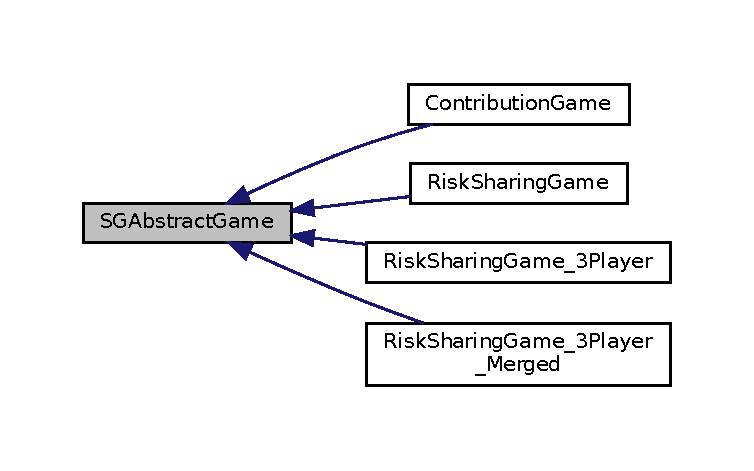
\includegraphics[width=350pt]{classSGAbstractGame__inherit__graph}
\end{center}
\end{figure}
\subsection*{Public Member Functions}
\begin{DoxyCompactItemize}
\item 
\mbox{\Hypertarget{classSGAbstractGame_a7a804027e8f7d5f718c78ffef6ef9195}\label{classSGAbstractGame_a7a804027e8f7d5f718c78ffef6ef9195}} 
\hyperlink{classSGAbstractGame_a7a804027e8f7d5f718c78ffef6ef9195}{S\+G\+Abstract\+Game} (int \+\_\+num\+Players, double \+\_\+delta, int \+\_\+num\+States, vector$<$ vector$<$ int $>$ $>$ \+\_\+num\+Actions)
\begin{DoxyCompactList}\small\item\em Constructor for the pure virtual class. \end{DoxyCompactList}\item 
\hyperlink{classSGAbstractGame_aa4d3130442e99f23f0ec78526629f0b4}{S\+G\+Abstract\+Game} (double \+\_\+delta, int \+\_\+num\+States, vector$<$ vector$<$ int $>$ $>$ \+\_\+num\+Actions)
\begin{DoxyCompactList}\small\item\em Constructor for the pure virtual class. \end{DoxyCompactList}\item 
virtual \hyperlink{classSGPoint}{S\+G\+Point} \hyperlink{classSGAbstractGame_a3fc1cd009d1813f44f1f219e7deb6eef}{payoffs} (int state, const vector$<$ int $>$ \&actions) const =0
\begin{DoxyCompactList}\small\item\em The payoff function. \end{DoxyCompactList}\item 
virtual double \hyperlink{classSGAbstractGame_a416b31d5020b75de49447ce4f7783b98}{probability} (int state, const vector$<$ int $>$ \&actions, int statep) const =0
\begin{DoxyCompactList}\small\item\em Transition probabilities. \end{DoxyCompactList}\item 
virtual bool \hyperlink{classSGAbstractGame_a2cec8147c3055cfe6314da349d1a7344}{is\+Equilibrium\+Action} (int state, const vector$<$ int $>$ \&actions) const
\item 
virtual bool \hyperlink{classSGAbstractGame_abd2542c0b2db7ed40d307f7f0a53048b}{constrained} (int player) const
\begin{DoxyCompactList}\small\item\em Returns true if the given player is incentive constrained. \end{DoxyCompactList}\item 
\hyperlink{classSGPoint}{S\+G\+Point} \hyperlink{classSGAbstractGame_a0373c95c41562ed3ce95b3406961b1ee}{payoffs} (int state, int action) const
\begin{DoxyCompactList}\small\item\em An overloaded version of payoffs that uses a linear action index. \end{DoxyCompactList}\item 
double \hyperlink{classSGAbstractGame_a922ec5b744295bf7d367f4df20f65b9f}{probability} (int state, int action, int statep) const
\item 
bool \hyperlink{classSGAbstractGame_aa7b88a879bd7b7aa7e275c0e0e92a3d8}{is\+Equilibrium\+Action} (int state, int action) const
\item 
\mbox{\Hypertarget{classSGAbstractGame_a16365eddd0af879c92ec17b47941fdee}\label{classSGAbstractGame_a16365eddd0af879c92ec17b47941fdee}} 
int \hyperlink{classSGAbstractGame_a16365eddd0af879c92ec17b47941fdee}{get\+Num\+Players} () const
\begin{DoxyCompactList}\small\item\em Returns the number of players. \end{DoxyCompactList}\item 
\mbox{\Hypertarget{classSGAbstractGame_adadae7cc528721461df1ea217c8dbba0}\label{classSGAbstractGame_adadae7cc528721461df1ea217c8dbba0}} 
double \hyperlink{classSGAbstractGame_adadae7cc528721461df1ea217c8dbba0}{get\+Delta} () const
\begin{DoxyCompactList}\small\item\em Returns the discount factor. \end{DoxyCompactList}\item 
\mbox{\Hypertarget{classSGAbstractGame_a02cf2b1cd5f86c44116bccc9dd17cdf7}\label{classSGAbstractGame_a02cf2b1cd5f86c44116bccc9dd17cdf7}} 
double \hyperlink{classSGAbstractGame_a02cf2b1cd5f86c44116bccc9dd17cdf7}{get\+Num\+States} () const
\begin{DoxyCompactList}\small\item\em Returns the number of states. \end{DoxyCompactList}\item 
\mbox{\Hypertarget{classSGAbstractGame_a2ec57d2920b8f88a238899dd5e203f1a}\label{classSGAbstractGame_a2ec57d2920b8f88a238899dd5e203f1a}} 
const vector$<$ vector$<$ int $>$ $>$ \hyperlink{classSGAbstractGame_a2ec57d2920b8f88a238899dd5e203f1a}{get\+Num\+Actions} () const
\begin{DoxyCompactList}\small\item\em Returns the number of actions array. \end{DoxyCompactList}\end{DoxyCompactItemize}
\subsection*{Protected Member Functions}
\begin{DoxyCompactItemize}
\item 
vector$<$ int $>$ \hyperlink{classSGAbstractGame_a1b1ab8f6b09aaef481ba8eab5934ac66}{index\+To\+Actions} (int index, int state) const
\begin{DoxyCompactList}\small\item\em Converts a linear index to multiindex. \end{DoxyCompactList}\end{DoxyCompactItemize}
\subsection*{Protected Attributes}
\begin{DoxyCompactItemize}
\item 
\mbox{\Hypertarget{classSGAbstractGame_aaa793d0ed9adcb2b2e11b999432bfae8}\label{classSGAbstractGame_aaa793d0ed9adcb2b2e11b999432bfae8}} 
int \hyperlink{classSGAbstractGame_aaa793d0ed9adcb2b2e11b999432bfae8}{num\+Players}
\begin{DoxyCompactList}\small\item\em The number of players, always 2. \end{DoxyCompactList}\item 
\mbox{\Hypertarget{classSGAbstractGame_a34c8905ac463bb2ec54aba4eb4ac376f}\label{classSGAbstractGame_a34c8905ac463bb2ec54aba4eb4ac376f}} 
double \hyperlink{classSGAbstractGame_a34c8905ac463bb2ec54aba4eb4ac376f}{delta}
\begin{DoxyCompactList}\small\item\em The discount factor. \end{DoxyCompactList}\item 
\mbox{\Hypertarget{classSGAbstractGame_a4d09150e3135b0abf07ae5319c12d1ef}\label{classSGAbstractGame_a4d09150e3135b0abf07ae5319c12d1ef}} 
int \hyperlink{classSGAbstractGame_a4d09150e3135b0abf07ae5319c12d1ef}{num\+States}
\begin{DoxyCompactList}\small\item\em The number of states. \end{DoxyCompactList}\item 
vector$<$ vector$<$ int $>$ $>$ \hyperlink{classSGAbstractGame_a907a945ec0afb42dfeb164b4520879c5}{num\+Actions}
\begin{DoxyCompactList}\small\item\em The numbers of actions in each state. \end{DoxyCompactList}\end{DoxyCompactItemize}


\subsection{Detailed Description}
A virtual class for constructing games. 

The \hyperlink{classSGGame}{S\+G\+Game} class has a constructor that constructs an \hyperlink{classSGGame}{S\+G\+Game} object from any class that inherits \hyperlink{classSGAbstractGame}{S\+G\+Abstract\+Game}. So you can inherit from this class as a convenience for building \hyperlink{classSGGame}{S\+G\+Game} objects. For an example of how this is done, see risksharing.\+hpp. The user provides definitions of a payoffs method and a probability method that return the flow payoffs of the players and the transition probabilities between states, respectively. The value in this is that the user can provide {\itshape rules} for how these quantities are generated, rather than having to generate {\itshape arrays} of these values for passing to the \hyperlink{classSGGame}{S\+G\+Game} constructor. See also \hyperlink{classSGGame_a935fc76700c675f842dc1666ffe2e8f7}{S\+G\+Game\+::\+S\+G\+Game}. 

\subsection{Constructor \& Destructor Documentation}
\mbox{\Hypertarget{classSGAbstractGame_aa4d3130442e99f23f0ec78526629f0b4}\label{classSGAbstractGame_aa4d3130442e99f23f0ec78526629f0b4}} 
\index{S\+G\+Abstract\+Game@{S\+G\+Abstract\+Game}!S\+G\+Abstract\+Game@{S\+G\+Abstract\+Game}}
\index{S\+G\+Abstract\+Game@{S\+G\+Abstract\+Game}!S\+G\+Abstract\+Game@{S\+G\+Abstract\+Game}}
\subsubsection{\texorpdfstring{S\+G\+Abstract\+Game()}{SGAbstractGame()}}
{\footnotesize\ttfamily S\+G\+Abstract\+Game\+::\+S\+G\+Abstract\+Game (\begin{DoxyParamCaption}\item[{double}]{\+\_\+delta,  }\item[{int}]{\+\_\+num\+States,  }\item[{vector$<$ vector$<$ int $>$ $>$}]{\+\_\+num\+Actions }\end{DoxyParamCaption})\hspace{0.3cm}{\ttfamily [inline]}}



Constructor for the pure virtual class. 

Grandfather in old code that is specialized to two players. 

\subsection{Member Function Documentation}
\mbox{\Hypertarget{classSGAbstractGame_abd2542c0b2db7ed40d307f7f0a53048b}\label{classSGAbstractGame_abd2542c0b2db7ed40d307f7f0a53048b}} 
\index{S\+G\+Abstract\+Game@{S\+G\+Abstract\+Game}!constrained@{constrained}}
\index{constrained@{constrained}!S\+G\+Abstract\+Game@{S\+G\+Abstract\+Game}}
\subsubsection{\texorpdfstring{constrained()}{constrained()}}
{\footnotesize\ttfamily virtual bool S\+G\+Abstract\+Game\+::constrained (\begin{DoxyParamCaption}\item[{int}]{player }\end{DoxyParamCaption}) const\hspace{0.3cm}{\ttfamily [inline]}, {\ttfamily [virtual]}}



Returns true if the given player is incentive constrained. 

The default definition of this method always returns true, so that both players\textquotesingle{} behavior is subject to incentive constraints. By making this method return false for one or both players, the user can implement models in which players can commit to their actions. When both players are not constrained, the algorithm will compute the feasible payoff correspondence. \mbox{\Hypertarget{classSGAbstractGame_a1b1ab8f6b09aaef481ba8eab5934ac66}\label{classSGAbstractGame_a1b1ab8f6b09aaef481ba8eab5934ac66}} 
\index{S\+G\+Abstract\+Game@{S\+G\+Abstract\+Game}!index\+To\+Actions@{index\+To\+Actions}}
\index{index\+To\+Actions@{index\+To\+Actions}!S\+G\+Abstract\+Game@{S\+G\+Abstract\+Game}}
\subsubsection{\texorpdfstring{index\+To\+Actions()}{indexToActions()}}
{\footnotesize\ttfamily vector$<$int$>$ S\+G\+Abstract\+Game\+::index\+To\+Actions (\begin{DoxyParamCaption}\item[{int}]{index,  }\item[{int}]{state }\end{DoxyParamCaption}) const\hspace{0.3cm}{\ttfamily [inline]}, {\ttfamily [protected]}}



Converts a linear index to multiindex. 

This function takes the linear index of an action pair in state s and returns a multiindex that gives each player\textquotesingle{}s action. \mbox{\Hypertarget{classSGAbstractGame_a2cec8147c3055cfe6314da349d1a7344}\label{classSGAbstractGame_a2cec8147c3055cfe6314da349d1a7344}} 
\index{S\+G\+Abstract\+Game@{S\+G\+Abstract\+Game}!is\+Equilibrium\+Action@{is\+Equilibrium\+Action}}
\index{is\+Equilibrium\+Action@{is\+Equilibrium\+Action}!S\+G\+Abstract\+Game@{S\+G\+Abstract\+Game}}
\subsubsection{\texorpdfstring{is\+Equilibrium\+Action()}{isEquilibriumAction()}\hspace{0.1cm}{\footnotesize\ttfamily [1/2]}}
{\footnotesize\ttfamily virtual bool S\+G\+Abstract\+Game\+::is\+Equilibrium\+Action (\begin{DoxyParamCaption}\item[{int}]{state,  }\item[{const vector$<$ int $>$ \&}]{actions }\end{DoxyParamCaption}) const\hspace{0.3cm}{\ttfamily [inline]}, {\ttfamily [virtual]}}

Returns true if the given action pair can be played in equilibrium

The default definition of this method always returns true, so that all action pairs can be played in equilibrium. By redefining this method, the user can create models in which only a subset of action pairs are played on the equilibrium path. 

Reimplemented in \hyperlink{classRiskSharingGame_a7da6b669317562cd9df8dfc0f8226b4c}{Risk\+Sharing\+Game}, \hyperlink{classRiskSharingGame__3Player_a79f44b04c558ecd72cf0b464fdd8a317}{Risk\+Sharing\+Game\+\_\+3\+Player}, and \hyperlink{classRiskSharingGame__3Player__Merged_aeff4f08e00ef46bbdbb190c9c6c393a4}{Risk\+Sharing\+Game\+\_\+3\+Player\+\_\+\+Merged}.

\mbox{\Hypertarget{classSGAbstractGame_aa7b88a879bd7b7aa7e275c0e0e92a3d8}\label{classSGAbstractGame_aa7b88a879bd7b7aa7e275c0e0e92a3d8}} 
\index{S\+G\+Abstract\+Game@{S\+G\+Abstract\+Game}!is\+Equilibrium\+Action@{is\+Equilibrium\+Action}}
\index{is\+Equilibrium\+Action@{is\+Equilibrium\+Action}!S\+G\+Abstract\+Game@{S\+G\+Abstract\+Game}}
\subsubsection{\texorpdfstring{is\+Equilibrium\+Action()}{isEquilibriumAction()}\hspace{0.1cm}{\footnotesize\ttfamily [2/2]}}
{\footnotesize\ttfamily bool S\+G\+Abstract\+Game\+::is\+Equilibrium\+Action (\begin{DoxyParamCaption}\item[{int}]{state,  }\item[{int}]{action }\end{DoxyParamCaption}) const\hspace{0.3cm}{\ttfamily [inline]}}

An overloaded version of is\+Equilibrium\+Action that uses a linear action index

This method converts the linear action index into an action pair and then returns the result of the user defined is\+Equilibrium\+Action method. \mbox{\Hypertarget{classSGAbstractGame_a3fc1cd009d1813f44f1f219e7deb6eef}\label{classSGAbstractGame_a3fc1cd009d1813f44f1f219e7deb6eef}} 
\index{S\+G\+Abstract\+Game@{S\+G\+Abstract\+Game}!payoffs@{payoffs}}
\index{payoffs@{payoffs}!S\+G\+Abstract\+Game@{S\+G\+Abstract\+Game}}
\subsubsection{\texorpdfstring{payoffs()}{payoffs()}\hspace{0.1cm}{\footnotesize\ttfamily [1/2]}}
{\footnotesize\ttfamily virtual \hyperlink{classSGPoint}{S\+G\+Point} S\+G\+Abstract\+Game\+::payoffs (\begin{DoxyParamCaption}\item[{int}]{state,  }\item[{const vector$<$ int $>$ \&}]{actions }\end{DoxyParamCaption}) const\hspace{0.3cm}{\ttfamily [pure virtual]}}



The payoff function. 

A class that is derived from \hyperlink{classSGAbstractGame}{S\+G\+Abstract\+Game} must define the payoffs method, which returns, for a given state and action pair, the flow payoffs that the players receive as an \hyperlink{classSGPoint}{S\+G\+Point}. 

Implemented in \hyperlink{classRiskSharingGame_a2aed9769b6518ed68b0c595629fb0129}{Risk\+Sharing\+Game}, \hyperlink{classRiskSharingGame__3Player_ae4a07f7dc66f18eccd29bc7993c0472f}{Risk\+Sharing\+Game\+\_\+3\+Player}, \hyperlink{classRiskSharingGame__3Player__Merged_aa1d807770ff356fe1114d17966172fbd}{Risk\+Sharing\+Game\+\_\+3\+Player\+\_\+\+Merged}, and \hyperlink{classContributionGame_ab33daef685ec7b22c44dad283c2f88cd}{Contribution\+Game}.

\mbox{\Hypertarget{classSGAbstractGame_a0373c95c41562ed3ce95b3406961b1ee}\label{classSGAbstractGame_a0373c95c41562ed3ce95b3406961b1ee}} 
\index{S\+G\+Abstract\+Game@{S\+G\+Abstract\+Game}!payoffs@{payoffs}}
\index{payoffs@{payoffs}!S\+G\+Abstract\+Game@{S\+G\+Abstract\+Game}}
\subsubsection{\texorpdfstring{payoffs()}{payoffs()}\hspace{0.1cm}{\footnotesize\ttfamily [2/2]}}
{\footnotesize\ttfamily \hyperlink{classSGPoint}{S\+G\+Point} S\+G\+Abstract\+Game\+::payoffs (\begin{DoxyParamCaption}\item[{int}]{state,  }\item[{int}]{action }\end{DoxyParamCaption}) const\hspace{0.3cm}{\ttfamily [inline]}}



An overloaded version of payoffs that uses a linear action index. 

This method converts the linear action index into an action pair and then returns the result of the user defined payoffs method. \mbox{\Hypertarget{classSGAbstractGame_a416b31d5020b75de49447ce4f7783b98}\label{classSGAbstractGame_a416b31d5020b75de49447ce4f7783b98}} 
\index{S\+G\+Abstract\+Game@{S\+G\+Abstract\+Game}!probability@{probability}}
\index{probability@{probability}!S\+G\+Abstract\+Game@{S\+G\+Abstract\+Game}}
\subsubsection{\texorpdfstring{probability()}{probability()}\hspace{0.1cm}{\footnotesize\ttfamily [1/2]}}
{\footnotesize\ttfamily virtual double S\+G\+Abstract\+Game\+::probability (\begin{DoxyParamCaption}\item[{int}]{state,  }\item[{const vector$<$ int $>$ \&}]{actions,  }\item[{int}]{statep }\end{DoxyParamCaption}) const\hspace{0.3cm}{\ttfamily [pure virtual]}}



Transition probabilities. 

A class that derives from \hyperlink{classSGAbstractGame}{S\+G\+Abstract\+Game} must define the probability method, which gives, for each state and action pair and new state, the probability of reaching the new state tomorrow when starting from the given state and when the given action pair is played. 

Implemented in \hyperlink{classRiskSharingGame_aa9ae41ec3aec3342ffd2d16187746718}{Risk\+Sharing\+Game}, \hyperlink{classRiskSharingGame__3Player_a48f478394bae9cf7479519da9b18a987}{Risk\+Sharing\+Game\+\_\+3\+Player}, \hyperlink{classRiskSharingGame__3Player__Merged_a505d06e31a1cabde1c6fab8ac5af8409}{Risk\+Sharing\+Game\+\_\+3\+Player\+\_\+\+Merged}, and \hyperlink{classContributionGame_a7b5ca7f6f0119f5899784ceae570666d}{Contribution\+Game}.

\mbox{\Hypertarget{classSGAbstractGame_a922ec5b744295bf7d367f4df20f65b9f}\label{classSGAbstractGame_a922ec5b744295bf7d367f4df20f65b9f}} 
\index{S\+G\+Abstract\+Game@{S\+G\+Abstract\+Game}!probability@{probability}}
\index{probability@{probability}!S\+G\+Abstract\+Game@{S\+G\+Abstract\+Game}}
\subsubsection{\texorpdfstring{probability()}{probability()}\hspace{0.1cm}{\footnotesize\ttfamily [2/2]}}
{\footnotesize\ttfamily double S\+G\+Abstract\+Game\+::probability (\begin{DoxyParamCaption}\item[{int}]{state,  }\item[{int}]{action,  }\item[{int}]{statep }\end{DoxyParamCaption}) const\hspace{0.3cm}{\ttfamily [inline]}}

An overloaded version of probability that uses a linear action index

This method converts the linear action index into an action pair and then returns the result of the user defined probability method. 

\subsection{Member Data Documentation}
\mbox{\Hypertarget{classSGAbstractGame_a907a945ec0afb42dfeb164b4520879c5}\label{classSGAbstractGame_a907a945ec0afb42dfeb164b4520879c5}} 
\index{S\+G\+Abstract\+Game@{S\+G\+Abstract\+Game}!num\+Actions@{num\+Actions}}
\index{num\+Actions@{num\+Actions}!S\+G\+Abstract\+Game@{S\+G\+Abstract\+Game}}
\subsubsection{\texorpdfstring{num\+Actions}{numActions}}
{\footnotesize\ttfamily vector$<$ vector$<$int$>$ $>$ S\+G\+Abstract\+Game\+::num\+Actions\hspace{0.3cm}{\ttfamily [protected]}}



The numbers of actions in each state. 

num\+Actions\mbox{[}s\mbox{]}\mbox{[}s\mbox{]} is the number of actions that player i can take in state s. 

The documentation for this class was generated from the following file\+:\begin{DoxyCompactItemize}
\item 
src/hpp/sgabstractgame.\+hpp\end{DoxyCompactItemize}

\hypertarget{classSGAction}{\section{S\-G\-Action Class Reference}
\label{classSGAction}\index{S\-G\-Action@{S\-G\-Action}}
}


Describes an action in the game.  




{\ttfamily \#include $<$sgaction.\-hpp$>$}

\subsection*{Public Member Functions}
\begin{DoxyCompactItemize}
\item 
\hypertarget{classSGAction_a763b30d91b4ac060895b3af2731d097c}{\hyperlink{classSGAction_a763b30d91b4ac060895b3af2731d097c}{S\-G\-Action} (const \hyperlink{classSGEnv}{S\-G\-Env} \&\-\_\-env, int \-\_\-state, int \-\_\-action)}\label{classSGAction_a763b30d91b4ac060895b3af2731d097c}

\begin{DoxyCompactList}\small\item\em Initializes the action with the given state/action. \end{DoxyCompactList}\item 
\hypertarget{classSGAction_a669309713ab99e375da193bbfa6fc586}{int \hyperlink{classSGAction_a669309713ab99e375da193bbfa6fc586}{get\-Action} () const }\label{classSGAction_a669309713ab99e375da193bbfa6fc586}

\begin{DoxyCompactList}\small\item\em Returns the action. \end{DoxyCompactList}\item 
\hypertarget{classSGAction_a279af062730a81a022177740112c5f2d}{int \hyperlink{classSGAction_a279af062730a81a022177740112c5f2d}{get\-State} () const }\label{classSGAction_a279af062730a81a022177740112c5f2d}

\begin{DoxyCompactList}\small\item\em Returns the state. \end{DoxyCompactList}\item 
\hypertarget{classSGAction_aa3758e5365a78ee447ec41914cc7bb99}{\hyperlink{classSGPoint}{S\-G\-Point} \hyperlink{classSGAction_aa3758e5365a78ee447ec41914cc7bb99}{get\-Min\-I\-C\-Payoffs} () const }\label{classSGAction_aa3758e5365a78ee447ec41914cc7bb99}

\begin{DoxyCompactList}\small\item\em Returns the minimum I\-C continuation values. \end{DoxyCompactList}\item 
void \hyperlink{classSGAction_a7ecafdb0cf42f83931f923f2e4e23f25}{intersect\-Ray} (const \hyperlink{classSGPoint}{S\-G\-Point} \&pivot, const \hyperlink{classSGPoint}{S\-G\-Point} \&direction)
\begin{DoxyCompactList}\small\item\em Trims binding continuation segments. \end{DoxyCompactList}\item 
\hypertarget{classSGAction_ae78f31d121e131788ac4c767e01d012c}{void \hyperlink{classSGAction_ae78f31d121e131788ac4c767e01d012c}{intersect\-Ray\-Segment} (const \hyperlink{classSGPoint}{S\-G\-Point} \&pivot, const \hyperlink{classSGPoint}{S\-G\-Point} \&direction, int player)}\label{classSGAction_ae78f31d121e131788ac4c767e01d012c}

\begin{DoxyCompactList}\small\item\em Static method to carry out trimming operations. \end{DoxyCompactList}\item 
\hypertarget{classSGAction_a2d1b9515be55e396e8595051ba6d3bdd}{{\footnotesize template$<$class Archive $>$ }\\void \hyperlink{classSGAction_a2d1b9515be55e396e8595051ba6d3bdd}{serialize} (Archive \&ar, const unsigned int version)}\label{classSGAction_a2d1b9515be55e396e8595051ba6d3bdd}

\begin{DoxyCompactList}\small\item\em Serializes the action using the boost\-::serialization library. \end{DoxyCompactList}\end{DoxyCompactItemize}
\subsection*{Protected Attributes}
\begin{DoxyCompactItemize}
\item 
const \hyperlink{classSGEnv}{S\-G\-Env} \& \hyperlink{classSGAction_a5ae60f6fd5a545d13c8a2525d7378b9d}{env}
\item 
int \hyperlink{classSGAction_a1ad4ae3feb4e3ec46e21273dd51a6004}{state}
\item 
int \hyperlink{classSGAction_a65c62a3804b50febd9a289f3d8902f85}{action}
\item 
\hyperlink{classSGPoint}{S\-G\-Point} \hyperlink{classSGAction_a20b96be3274e3cd2bc1be0d218fc2b06}{min\-I\-C}
\item 
vector$<$ \hyperlink{classSGTuple}{S\-G\-Tuple} $>$ \hyperlink{classSGAction_a8860ada2cacece1a8feed794d81d9e9f}{points}
\item 
vector$<$ vector$<$ int $>$ $>$ \hyperlink{classSGAction_a60599bc5a745db1557191a61c0db28b3}{tuples}
\end{DoxyCompactItemize}
\subsection*{Friends}
\begin{DoxyCompactItemize}
\item 
\hypertarget{classSGAction_ac98d07dd8f7b70e16ccb9a01abf56b9c}{class {\bfseries boost\-::serialization\-::access}}\label{classSGAction_ac98d07dd8f7b70e16ccb9a01abf56b9c}

\item 
\hypertarget{classSGAction_a80adcf9eac5da53e729646c94d3b8f1d}{class {\bfseries S\-G\-Approx}}\label{classSGAction_a80adcf9eac5da53e729646c94d3b8f1d}

\end{DoxyCompactItemize}


\subsection{Detailed Description}
Describes an action in the game. 

\begin{DoxyVerb}Stores IC region information for a single action. Stores the
\end{DoxyVerb}
 action, minimum incentive compatible payoffs, points of intersection between the I\-C region and the expected feasible set, and indices of the tuples that generate the points of intersection. 

\subsection{Member Function Documentation}
\hypertarget{classSGAction_a7ecafdb0cf42f83931f923f2e4e23f25}{\index{S\-G\-Action@{S\-G\-Action}!intersect\-Ray@{intersect\-Ray}}
\index{intersect\-Ray@{intersect\-Ray}!SGAction@{S\-G\-Action}}
\subsubsection[{intersect\-Ray}]{\setlength{\rightskip}{0pt plus 5cm}void S\-G\-Action\-::intersect\-Ray (
\begin{DoxyParamCaption}
\item[{const {\bf S\-G\-Point} \&}]{pivot, }
\item[{const {\bf S\-G\-Point} \&}]{direction}
\end{DoxyParamCaption}
)}}\label{classSGAction_a7ecafdb0cf42f83931f923f2e4e23f25}


Trims binding continuation segments. 

Intersects the binding continuation segments in \hyperlink{classSGAction_a8860ada2cacece1a8feed794d81d9e9f}{S\-G\-Action\-::points} with the half space that is below pivot in direction.\-get\-Normal(). 

\subsection{Member Data Documentation}
\hypertarget{classSGAction_a65c62a3804b50febd9a289f3d8902f85}{\index{S\-G\-Action@{S\-G\-Action}!action@{action}}
\index{action@{action}!SGAction@{S\-G\-Action}}
\subsubsection[{action}]{\setlength{\rightskip}{0pt plus 5cm}int S\-G\-Action\-::action\hspace{0.3cm}{\ttfamily [protected]}}}\label{classSGAction_a65c62a3804b50febd9a289f3d8902f85}
The index of the action profile. \hypertarget{classSGAction_a5ae60f6fd5a545d13c8a2525d7378b9d}{\index{S\-G\-Action@{S\-G\-Action}!env@{env}}
\index{env@{env}!SGAction@{S\-G\-Action}}
\subsubsection[{env}]{\setlength{\rightskip}{0pt plus 5cm}const {\bf S\-G\-Env}\& S\-G\-Action\-::env\hspace{0.3cm}{\ttfamily [protected]}}}\label{classSGAction_a5ae60f6fd5a545d13c8a2525d7378b9d}
Constant reference to the parent environment. \hypertarget{classSGAction_a20b96be3274e3cd2bc1be0d218fc2b06}{\index{S\-G\-Action@{S\-G\-Action}!min\-I\-C@{min\-I\-C}}
\index{min\-I\-C@{min\-I\-C}!SGAction@{S\-G\-Action}}
\subsubsection[{min\-I\-C}]{\setlength{\rightskip}{0pt plus 5cm}{\bf S\-G\-Point} S\-G\-Action\-::min\-I\-C\hspace{0.3cm}{\ttfamily [protected]}}}\label{classSGAction_a20b96be3274e3cd2bc1be0d218fc2b06}
The minimum continuation value to support incentive compatibility, relative to the current threat tuple. In particular, this is the maximum over all deviations of the expected threat point under the deviation, plus (1-\/delta)/delta times the static gains from deviating. \hypertarget{classSGAction_a8860ada2cacece1a8feed794d81d9e9f}{\index{S\-G\-Action@{S\-G\-Action}!points@{points}}
\index{points@{points}!SGAction@{S\-G\-Action}}
\subsubsection[{points}]{\setlength{\rightskip}{0pt plus 5cm}vector$<$ {\bf S\-G\-Tuple} $>$ S\-G\-Action\-::points\hspace{0.3cm}{\ttfamily [protected]}}}\label{classSGAction_a8860ada2cacece1a8feed794d81d9e9f}
Extreme points of the set of expected feasible continuation values at which some player's incentive constraint binds. points\mbox{[}i\mbox{]} is an \hyperlink{classSGTuple}{S\-G\-Tuple} consisting of either 0 or 2 \hyperlink{classSGPoint}{S\-G\-Point} objects, which are the extreme binding payoffs on player i's incentive constraint. The convention is that the first element of the tuple is the northern or easternmost of the two binding payoffs. \hypertarget{classSGAction_a1ad4ae3feb4e3ec46e21273dd51a6004}{\index{S\-G\-Action@{S\-G\-Action}!state@{state}}
\index{state@{state}!SGAction@{S\-G\-Action}}
\subsubsection[{state}]{\setlength{\rightskip}{0pt plus 5cm}int S\-G\-Action\-::state\hspace{0.3cm}{\ttfamily [protected]}}}\label{classSGAction_a1ad4ae3feb4e3ec46e21273dd51a6004}
The state in which this action profile can be played. \hypertarget{classSGAction_a60599bc5a745db1557191a61c0db28b3}{\index{S\-G\-Action@{S\-G\-Action}!tuples@{tuples}}
\index{tuples@{tuples}!SGAction@{S\-G\-Action}}
\subsubsection[{tuples}]{\setlength{\rightskip}{0pt plus 5cm}vector$<$ vector$<$ int $>$ $>$ S\-G\-Action\-::tuples\hspace{0.3cm}{\ttfamily [protected]}}}\label{classSGAction_a60599bc5a745db1557191a61c0db28b3}
The vector tuples\mbox{[}i\mbox{]}\mbox{[}j\mbox{]} points to the element of S\-G\-Approximation\-::extreme\-Tuples whose expectation is just clockwise relative to points\mbox{[}i\mbox{]}\mbox{[}j\mbox{]}. 

The documentation for this class was generated from the following files\-:\begin{DoxyCompactItemize}
\item 
src/hpp/sgaction.\-hpp\item 
src/cpp/sgaction.\-cpp\end{DoxyCompactItemize}

\hypertarget{classSGAction__MaxMinMax}{}\section{S\+G\+Action\+\_\+\+Max\+Min\+Max Class Reference}
\label{classSGAction__MaxMinMax}\index{S\+G\+Action\+\_\+\+Max\+Min\+Max@{S\+G\+Action\+\_\+\+Max\+Min\+Max}}


Enhanced version of \hyperlink{classSGBaseAction}{S\+G\+Base\+Action}.  




{\ttfamily \#include $<$sgaction\+\_\+maxminmax.\+hpp$>$}



Inheritance diagram for S\+G\+Action\+\_\+\+Max\+Min\+Max\+:
\nopagebreak
\begin{figure}[H]
\begin{center}
\leavevmode
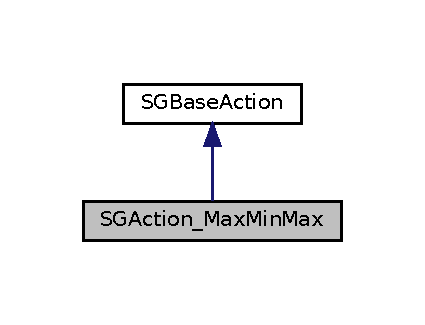
\includegraphics[width=204pt]{classSGAction__MaxMinMax__inherit__graph}
\end{center}
\end{figure}


Collaboration diagram for S\+G\+Action\+\_\+\+Max\+Min\+Max\+:
\nopagebreak
\begin{figure}[H]
\begin{center}
\leavevmode
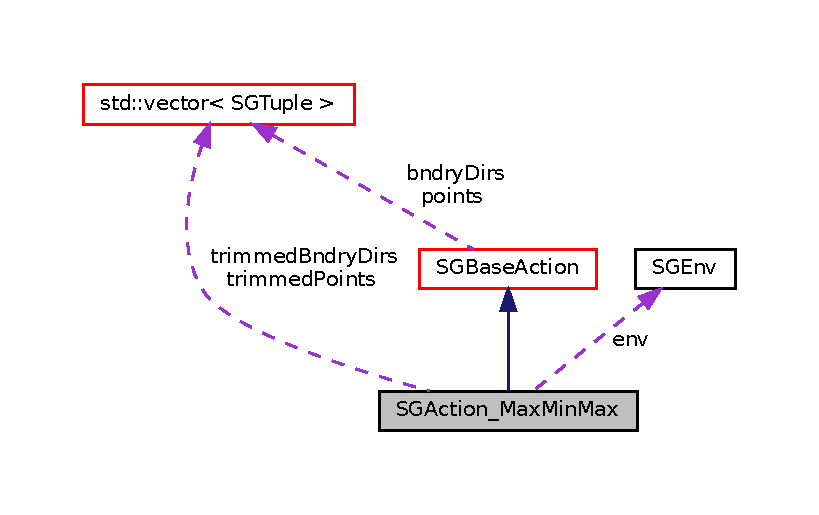
\includegraphics[width=350pt]{classSGAction__MaxMinMax__coll__graph}
\end{center}
\end{figure}
\subsection*{Public Member Functions}
\begin{DoxyCompactItemize}
\item 
\mbox{\Hypertarget{classSGAction__MaxMinMax_a4735732a1624affa09ac6ad1e2477431}\label{classSGAction__MaxMinMax_a4735732a1624affa09ac6ad1e2477431}} 
\hyperlink{classSGAction__MaxMinMax_a4735732a1624affa09ac6ad1e2477431}{S\+G\+Action\+\_\+\+Max\+Min\+Max} ()
\begin{DoxyCompactList}\small\item\em Default constructor. \end{DoxyCompactList}\item 
\hyperlink{classSGAction__MaxMinMax_a1183e22784f865a0478679874a77425e}{S\+G\+Action\+\_\+\+Max\+Min\+Max} (const \hyperlink{classSGEnv}{S\+G\+Env} \&\+\_\+env)
\begin{DoxyCompactList}\small\item\em Constructor. \end{DoxyCompactList}\item 
\hyperlink{classSGAction__MaxMinMax_a51894e40e19b3ec7d90b120f4fada9ed}{S\+G\+Action\+\_\+\+Max\+Min\+Max} (const \hyperlink{classSGEnv}{S\+G\+Env} \&\+\_\+env, int \+\_\+state, int \+\_\+action)
\begin{DoxyCompactList}\small\item\em Constructor. \end{DoxyCompactList}\item 
\hyperlink{classSGAction__MaxMinMax_a7d01d987f83c851e19d3620a27a4d8b0}{S\+G\+Action\+\_\+\+Max\+Min\+Max} (const \hyperlink{classSGEnv}{S\+G\+Env} \&\+\_\+env, int \+\_\+num\+Players, int \+\_\+state, int \+\_\+action)
\begin{DoxyCompactList}\small\item\em Constructor. \end{DoxyCompactList}\item 
void \hyperlink{classSGAction__MaxMinMax_ae7e17727071ae5257c6f28bb5eeb1972}{reset\+Trimmed\+Points} ()
\begin{DoxyCompactList}\small\item\em Resets the trimmed points for two players. \end{DoxyCompactList}\item 
void \hyperlink{classSGAction__MaxMinMax_a76943bc1614a4e3abe153ca6b12faf7c}{reset\+Trimmed\+Points} (const \hyperlink{classSGPoint}{S\+G\+Point} \&payoff\+UB)
\begin{DoxyCompactList}\small\item\em Resets the trimmed points for three players. \end{DoxyCompactList}\item 
\mbox{\Hypertarget{classSGAction__MaxMinMax_abb81ccc819f0f17cb90c64dad7af3d41}\label{classSGAction__MaxMinMax_abb81ccc819f0f17cb90c64dad7af3d41}} 
void \hyperlink{classSGAction__MaxMinMax_abb81ccc819f0f17cb90c64dad7af3d41}{update\+Trim} ()
\begin{DoxyCompactList}\small\item\em Sets points equal to the trimmed points. \end{DoxyCompactList}\item 
\mbox{\Hypertarget{classSGAction__MaxMinMax_a882cc59e96c325d7339cf28ee6bf63a5}\label{classSGAction__MaxMinMax_a882cc59e96c325d7339cf28ee6bf63a5}} 
double \hyperlink{classSGAction__MaxMinMax_a882cc59e96c325d7339cf28ee6bf63a5}{dist\+To\+Trimmed} () const
\begin{DoxyCompactList}\small\item\em Calculates the distance between points and trimmed\+Points in the sup norm. \end{DoxyCompactList}\item 
\mbox{\Hypertarget{classSGAction__MaxMinMax_a6a7c5c65a4b8c80e919dbb0039a3831c}\label{classSGAction__MaxMinMax_a6a7c5c65a4b8c80e919dbb0039a3831c}} 
bool \hyperlink{classSGAction__MaxMinMax_a6a7c5c65a4b8c80e919dbb0039a3831c}{intersect\+Half\+Space} (const \hyperlink{classSGPoint}{S\+G\+Point} \&normal, const double level, int player, \hyperlink{classSGTuple}{S\+G\+Tuple} \&segment, \hyperlink{classSGTuple}{S\+G\+Tuple} \&segment\+Dirs)
\begin{DoxyCompactList}\small\item\em Intersects the segment with a half space. \end{DoxyCompactList}\item 
\mbox{\Hypertarget{classSGAction__MaxMinMax_ada49ec584361e9ec63b16f22f8d57468}\label{classSGAction__MaxMinMax_ada49ec584361e9ec63b16f22f8d57468}} 
bool \hyperlink{classSGAction__MaxMinMax_ada49ec584361e9ec63b16f22f8d57468}{intersect\+Polygon\+Half\+Space} (const \hyperlink{classSGPoint}{S\+G\+Point} \&normal, const double level, int player, \hyperlink{classSGTuple}{S\+G\+Tuple} \&ext\+Pnts, \hyperlink{classSGTuple}{S\+G\+Tuple} \&ext\+Pnt\+Dirs)
\begin{DoxyCompactList}\small\item\em Intersects the IC polygon with a half space. \end{DoxyCompactList}\item 
bool \hyperlink{classSGAction__MaxMinMax_a15466a06d5b9bdce97eaa20f9fa94371}{trim} (const \hyperlink{classSGPoint}{S\+G\+Point} \&normal, double level)
\begin{DoxyCompactList}\small\item\em Trims the trimmed\+Points using intersect\+Ray\+Segment. \end{DoxyCompactList}\item 
\mbox{\Hypertarget{classSGAction__MaxMinMax_a436f348d7f24cd28a029f25e94aadf8a}\label{classSGAction__MaxMinMax_a436f348d7f24cd28a029f25e94aadf8a}} 
void \hyperlink{classSGAction__MaxMinMax_a436f348d7f24cd28a029f25e94aadf8a}{merge\+Duplicate\+Points} (const double tol)
\begin{DoxyCompactList}\small\item\em Merges duplicates up to the given tolerance. \end{DoxyCompactList}\item 
\mbox{\Hypertarget{classSGAction__MaxMinMax_a38b72633733d68122a63ee366eb11e64}\label{classSGAction__MaxMinMax_a38b72633733d68122a63ee366eb11e64}} 
void \hyperlink{classSGAction__MaxMinMax_a38b72633733d68122a63ee366eb11e64}{calculate\+Min\+IC} (const \hyperlink{classSGGame}{S\+G\+Game} \&game, const vector$<$ bool $>$ \&update, const \hyperlink{classSGTuple}{S\+G\+Tuple} \&threat\+Tuple)
\begin{DoxyCompactList}\small\item\em Calculates the minimum incentive compatible continuation payoff. \end{DoxyCompactList}\item 
\mbox{\Hypertarget{classSGAction__MaxMinMax_a446205895c561c6f54388b63a4a5e39c}\label{classSGAction__MaxMinMax_a446205895c561c6f54388b63a4a5e39c}} 
void \hyperlink{classSGAction__MaxMinMax_a446205895c561c6f54388b63a4a5e39c}{calculate\+Min\+IC} (const \hyperlink{classSGGame}{S\+G\+Game} \&game, const \hyperlink{classSGTuple}{S\+G\+Tuple} \&threat\+Tuple)
\begin{DoxyCompactList}\small\item\em Calculates the minimum incentive compatible continuation payoff. \end{DoxyCompactList}\item 
\mbox{\Hypertarget{classSGAction__MaxMinMax_ae64c1a8a37df28b0df8ca9b7ea1a51b9}\label{classSGAction__MaxMinMax_ae64c1a8a37df28b0df8ca9b7ea1a51b9}} 
const vector$<$ \hyperlink{classSGTuple}{S\+G\+Tuple} $>$ \& \hyperlink{classSGAction__MaxMinMax_ae64c1a8a37df28b0df8ca9b7ea1a51b9}{get\+Trimmed\+Points} () const
\begin{DoxyCompactList}\small\item\em Get method for trimmed points. \end{DoxyCompactList}\item 
\mbox{\Hypertarget{classSGAction__MaxMinMax_a92231e303ea20977d0aa7339c60d9c08}\label{classSGAction__MaxMinMax_a92231e303ea20977d0aa7339c60d9c08}} 
const vector$<$ \hyperlink{classSGTuple}{S\+G\+Tuple} $>$ \& \hyperlink{classSGAction__MaxMinMax_a92231e303ea20977d0aa7339c60d9c08}{get\+Trimmed\+Bndry\+Dirs} () const
\begin{DoxyCompactList}\small\item\em Get method for trimmed points. \end{DoxyCompactList}\item 
const \hyperlink{classSGPoint}{S\+G\+Point} \hyperlink{classSGAction__MaxMinMax_a2d4762138486ac532de10879eaa2008f}{get\+Bndry\+Dir} (const int player, const int point) const
\begin{DoxyCompactList}\small\item\em Get boundary direction for 3 players. \end{DoxyCompactList}\item 
\mbox{\Hypertarget{classSGAction__MaxMinMax_a93a9b06f1189763352928ec3c700168f}\label{classSGAction__MaxMinMax_a93a9b06f1189763352928ec3c700168f}} 
bool {\bfseries supportable} (const \hyperlink{classSGPoint}{S\+G\+Point} \&feasible\+Point) const
\end{DoxyCompactItemize}
\subsection*{Static Public Member Functions}
\begin{DoxyCompactItemize}
\item 
static double \hyperlink{classSGAction__MaxMinMax_ab91331990288c649ba911c0eda28df3f}{calculate\+Min\+IC} (int \hyperlink{classSGBaseAction_af293adc10da2dbb5a388a2fbcca0c67c}{action}, int \hyperlink{classSGBaseAction_a2301bf142f93f7d3ddedd44676d10c6a}{state}, int player, const \hyperlink{classSGGame}{S\+G\+Game} \&game, const \hyperlink{classSGTuple}{S\+G\+Tuple} \&threat\+Tuple)
\begin{DoxyCompactList}\small\item\em Calculates the IC constraint. \end{DoxyCompactList}\end{DoxyCompactItemize}
\subsection*{Private Attributes}
\begin{DoxyCompactItemize}
\item 
const \hyperlink{classSGEnv}{S\+G\+Env} $\ast$ \hyperlink{classSGAction__MaxMinMax_a02879e7551a4d8f89d4dece73df79e8e}{env}
\item 
vector$<$ \hyperlink{classSGTuple}{S\+G\+Tuple} $>$ \hyperlink{classSGAction__MaxMinMax_aff074b8925e0e4efbe729a1fa760b574}{trimmed\+Points}
\item 
vector$<$ \hyperlink{classSGTuple}{S\+G\+Tuple} $>$ \hyperlink{classSGAction__MaxMinMax_a775fcd57afc142655d881205242b05b6}{trimmed\+Bndry\+Dirs}
\end{DoxyCompactItemize}
\subsection*{Additional Inherited Members}


\subsection{Detailed Description}
Enhanced version of \hyperlink{classSGBaseAction}{S\+G\+Base\+Action}. 

Same functionality as \hyperlink{classSGBaseAction}{S\+G\+Base\+Action}, but includes additional methods for computing payoffs and a reference to a parent \hyperlink{classSGEnv}{S\+G\+Env} object to control parameters for the computation.

This class is used by \hyperlink{classSGSolver__MaxMinMax}{S\+G\+Solver\+\_\+\+Max\+Min\+Max} to implement the max-\/min-\/max algorithm. 

\subsection{Constructor \& Destructor Documentation}
\mbox{\Hypertarget{classSGAction__MaxMinMax_a1183e22784f865a0478679874a77425e}\label{classSGAction__MaxMinMax_a1183e22784f865a0478679874a77425e}} 
\index{S\+G\+Action\+\_\+\+Max\+Min\+Max@{S\+G\+Action\+\_\+\+Max\+Min\+Max}!S\+G\+Action\+\_\+\+Max\+Min\+Max@{S\+G\+Action\+\_\+\+Max\+Min\+Max}}
\index{S\+G\+Action\+\_\+\+Max\+Min\+Max@{S\+G\+Action\+\_\+\+Max\+Min\+Max}!S\+G\+Action\+\_\+\+Max\+Min\+Max@{S\+G\+Action\+\_\+\+Max\+Min\+Max}}
\subsubsection{\texorpdfstring{S\+G\+Action\+\_\+\+Max\+Min\+Max()}{SGAction\_MaxMinMax()}\hspace{0.1cm}{\footnotesize\ttfamily [1/3]}}
{\footnotesize\ttfamily S\+G\+Action\+\_\+\+Max\+Min\+Max\+::\+S\+G\+Action\+\_\+\+Max\+Min\+Max (\begin{DoxyParamCaption}\item[{const \hyperlink{classSGEnv}{S\+G\+Env} \&}]{\+\_\+env }\end{DoxyParamCaption})\hspace{0.3cm}{\ttfamily [inline]}}



Constructor. 

Constructs a null action associated with the given \hyperlink{classSGEnv}{S\+G\+Env}. \mbox{\Hypertarget{classSGAction__MaxMinMax_a51894e40e19b3ec7d90b120f4fada9ed}\label{classSGAction__MaxMinMax_a51894e40e19b3ec7d90b120f4fada9ed}} 
\index{S\+G\+Action\+\_\+\+Max\+Min\+Max@{S\+G\+Action\+\_\+\+Max\+Min\+Max}!S\+G\+Action\+\_\+\+Max\+Min\+Max@{S\+G\+Action\+\_\+\+Max\+Min\+Max}}
\index{S\+G\+Action\+\_\+\+Max\+Min\+Max@{S\+G\+Action\+\_\+\+Max\+Min\+Max}!S\+G\+Action\+\_\+\+Max\+Min\+Max@{S\+G\+Action\+\_\+\+Max\+Min\+Max}}
\subsubsection{\texorpdfstring{S\+G\+Action\+\_\+\+Max\+Min\+Max()}{SGAction\_MaxMinMax()}\hspace{0.1cm}{\footnotesize\ttfamily [2/3]}}
{\footnotesize\ttfamily S\+G\+Action\+\_\+\+Max\+Min\+Max\+::\+S\+G\+Action\+\_\+\+Max\+Min\+Max (\begin{DoxyParamCaption}\item[{const \hyperlink{classSGEnv}{S\+G\+Env} \&}]{\+\_\+env,  }\item[{int}]{\+\_\+state,  }\item[{int}]{\+\_\+action }\end{DoxyParamCaption})\hspace{0.3cm}{\ttfamily [inline]}}



Constructor. 

Grandfather in old two player code. \mbox{\Hypertarget{classSGAction__MaxMinMax_a7d01d987f83c851e19d3620a27a4d8b0}\label{classSGAction__MaxMinMax_a7d01d987f83c851e19d3620a27a4d8b0}} 
\index{S\+G\+Action\+\_\+\+Max\+Min\+Max@{S\+G\+Action\+\_\+\+Max\+Min\+Max}!S\+G\+Action\+\_\+\+Max\+Min\+Max@{S\+G\+Action\+\_\+\+Max\+Min\+Max}}
\index{S\+G\+Action\+\_\+\+Max\+Min\+Max@{S\+G\+Action\+\_\+\+Max\+Min\+Max}!S\+G\+Action\+\_\+\+Max\+Min\+Max@{S\+G\+Action\+\_\+\+Max\+Min\+Max}}
\subsubsection{\texorpdfstring{S\+G\+Action\+\_\+\+Max\+Min\+Max()}{SGAction\_MaxMinMax()}\hspace{0.1cm}{\footnotesize\ttfamily [3/3]}}
{\footnotesize\ttfamily S\+G\+Action\+\_\+\+Max\+Min\+Max\+::\+S\+G\+Action\+\_\+\+Max\+Min\+Max (\begin{DoxyParamCaption}\item[{const \hyperlink{classSGEnv}{S\+G\+Env} \&}]{\+\_\+env,  }\item[{int}]{\+\_\+num\+Players,  }\item[{int}]{\+\_\+state,  }\item[{int}]{\+\_\+action }\end{DoxyParamCaption})\hspace{0.3cm}{\ttfamily [inline]}}



Constructor. 

Constructs an action for the given state and action index in the given environment. 

\subsection{Member Function Documentation}
\mbox{\Hypertarget{classSGAction__MaxMinMax_ab91331990288c649ba911c0eda28df3f}\label{classSGAction__MaxMinMax_ab91331990288c649ba911c0eda28df3f}} 
\index{S\+G\+Action\+\_\+\+Max\+Min\+Max@{S\+G\+Action\+\_\+\+Max\+Min\+Max}!calculate\+Min\+IC@{calculate\+Min\+IC}}
\index{calculate\+Min\+IC@{calculate\+Min\+IC}!S\+G\+Action\+\_\+\+Max\+Min\+Max@{S\+G\+Action\+\_\+\+Max\+Min\+Max}}
\subsubsection{\texorpdfstring{calculate\+Min\+I\+C()}{calculateMinIC()}}
{\footnotesize\ttfamily double S\+G\+Action\+\_\+\+Max\+Min\+Max\+::calculate\+Min\+IC (\begin{DoxyParamCaption}\item[{int}]{action,  }\item[{int}]{state,  }\item[{int}]{player,  }\item[{const \hyperlink{classSGGame}{S\+G\+Game} \&}]{game,  }\item[{const \hyperlink{classSGTuple}{S\+G\+Tuple} \&}]{threat\+Tuple }\end{DoxyParamCaption})\hspace{0.3cm}{\ttfamily [static]}}



Calculates the IC constraint. 

Calculates the minimum incentive compatible expected continuation value for the given action, relative to the given threat tuple and for the given \hyperlink{classSGGame}{S\+G\+Game}. \mbox{\Hypertarget{classSGAction__MaxMinMax_a2d4762138486ac532de10879eaa2008f}\label{classSGAction__MaxMinMax_a2d4762138486ac532de10879eaa2008f}} 
\index{S\+G\+Action\+\_\+\+Max\+Min\+Max@{S\+G\+Action\+\_\+\+Max\+Min\+Max}!get\+Bndry\+Dir@{get\+Bndry\+Dir}}
\index{get\+Bndry\+Dir@{get\+Bndry\+Dir}!S\+G\+Action\+\_\+\+Max\+Min\+Max@{S\+G\+Action\+\_\+\+Max\+Min\+Max}}
\subsubsection{\texorpdfstring{get\+Bndry\+Dir()}{getBndryDir()}}
{\footnotesize\ttfamily const \hyperlink{classSGPoint}{S\+G\+Point} S\+G\+Action\+\_\+\+Max\+Min\+Max\+::get\+Bndry\+Dir (\begin{DoxyParamCaption}\item[{const int}]{player,  }\item[{const int}]{point }\end{DoxyParamCaption}) const}



Get boundary direction for 3 players. 

$<$ Returns the cross product of the boundary directions at the given point, i.\+e., the direction along an edge of the boundary that points into the feasible and IC region. Only works for three players. \mbox{\Hypertarget{classSGAction__MaxMinMax_ae7e17727071ae5257c6f28bb5eeb1972}\label{classSGAction__MaxMinMax_ae7e17727071ae5257c6f28bb5eeb1972}} 
\index{S\+G\+Action\+\_\+\+Max\+Min\+Max@{S\+G\+Action\+\_\+\+Max\+Min\+Max}!reset\+Trimmed\+Points@{reset\+Trimmed\+Points}}
\index{reset\+Trimmed\+Points@{reset\+Trimmed\+Points}!S\+G\+Action\+\_\+\+Max\+Min\+Max@{S\+G\+Action\+\_\+\+Max\+Min\+Max}}
\subsubsection{\texorpdfstring{reset\+Trimmed\+Points()}{resetTrimmedPoints()}\hspace{0.1cm}{\footnotesize\ttfamily [1/2]}}
{\footnotesize\ttfamily void S\+G\+Action\+\_\+\+Max\+Min\+Max\+::reset\+Trimmed\+Points (\begin{DoxyParamCaption}{ }\end{DoxyParamCaption})}



Resets the trimmed points for two players. 

$<$ Sets the trimmed points to rays that point from the minimum incentive compatible continuation value along the positive coordinate axes. \mbox{\Hypertarget{classSGAction__MaxMinMax_a76943bc1614a4e3abe153ca6b12faf7c}\label{classSGAction__MaxMinMax_a76943bc1614a4e3abe153ca6b12faf7c}} 
\index{S\+G\+Action\+\_\+\+Max\+Min\+Max@{S\+G\+Action\+\_\+\+Max\+Min\+Max}!reset\+Trimmed\+Points@{reset\+Trimmed\+Points}}
\index{reset\+Trimmed\+Points@{reset\+Trimmed\+Points}!S\+G\+Action\+\_\+\+Max\+Min\+Max@{S\+G\+Action\+\_\+\+Max\+Min\+Max}}
\subsubsection{\texorpdfstring{reset\+Trimmed\+Points()}{resetTrimmedPoints()}\hspace{0.1cm}{\footnotesize\ttfamily [2/2]}}
{\footnotesize\ttfamily void S\+G\+Action\+\_\+\+Max\+Min\+Max\+::reset\+Trimmed\+Points (\begin{DoxyParamCaption}\item[{const \hyperlink{classSGPoint}{S\+G\+Point} \&}]{payoff\+UB }\end{DoxyParamCaption})}



Resets the trimmed points for three players. 

$<$ Sets the trimmed points to a large box in the coordinate plane between the minimum incentive compatible payoff and the payoff upper bound. \mbox{\Hypertarget{classSGAction__MaxMinMax_a15466a06d5b9bdce97eaa20f9fa94371}\label{classSGAction__MaxMinMax_a15466a06d5b9bdce97eaa20f9fa94371}} 
\index{S\+G\+Action\+\_\+\+Max\+Min\+Max@{S\+G\+Action\+\_\+\+Max\+Min\+Max}!trim@{trim}}
\index{trim@{trim}!S\+G\+Action\+\_\+\+Max\+Min\+Max@{S\+G\+Action\+\_\+\+Max\+Min\+Max}}
\subsubsection{\texorpdfstring{trim()}{trim()}}
{\footnotesize\ttfamily bool S\+G\+Action\+\_\+\+Max\+Min\+Max\+::trim (\begin{DoxyParamCaption}\item[{const \hyperlink{classSGPoint}{S\+G\+Point} \&}]{normal,  }\item[{double}]{level }\end{DoxyParamCaption})}



Trims the trimmed\+Points using intersect\+Ray\+Segment. 

$<$ Returns true if the action was actually trimmed. 

\subsection{Member Data Documentation}
\mbox{\Hypertarget{classSGAction__MaxMinMax_a02879e7551a4d8f89d4dece73df79e8e}\label{classSGAction__MaxMinMax_a02879e7551a4d8f89d4dece73df79e8e}} 
\index{S\+G\+Action\+\_\+\+Max\+Min\+Max@{S\+G\+Action\+\_\+\+Max\+Min\+Max}!env@{env}}
\index{env@{env}!S\+G\+Action\+\_\+\+Max\+Min\+Max@{S\+G\+Action\+\_\+\+Max\+Min\+Max}}
\subsubsection{\texorpdfstring{env}{env}}
{\footnotesize\ttfamily const \hyperlink{classSGEnv}{S\+G\+Env}$\ast$ S\+G\+Action\+\_\+\+Max\+Min\+Max\+::env\hspace{0.3cm}{\ttfamily [private]}}

Pointer to the parent environment. \mbox{\Hypertarget{classSGAction__MaxMinMax_a775fcd57afc142655d881205242b05b6}\label{classSGAction__MaxMinMax_a775fcd57afc142655d881205242b05b6}} 
\index{S\+G\+Action\+\_\+\+Max\+Min\+Max@{S\+G\+Action\+\_\+\+Max\+Min\+Max}!trimmed\+Bndry\+Dirs@{trimmed\+Bndry\+Dirs}}
\index{trimmed\+Bndry\+Dirs@{trimmed\+Bndry\+Dirs}!S\+G\+Action\+\_\+\+Max\+Min\+Max@{S\+G\+Action\+\_\+\+Max\+Min\+Max}}
\subsubsection{\texorpdfstring{trimmed\+Bndry\+Dirs}{trimmedBndryDirs}}
{\footnotesize\ttfamily vector$<$\hyperlink{classSGTuple}{S\+G\+Tuple}$>$ S\+G\+Action\+\_\+\+Max\+Min\+Max\+::trimmed\+Bndry\+Dirs\hspace{0.3cm}{\ttfamily [private]}}

Stores the boundary directions for the trimmed points. \mbox{\Hypertarget{classSGAction__MaxMinMax_aff074b8925e0e4efbe729a1fa760b574}\label{classSGAction__MaxMinMax_aff074b8925e0e4efbe729a1fa760b574}} 
\index{S\+G\+Action\+\_\+\+Max\+Min\+Max@{S\+G\+Action\+\_\+\+Max\+Min\+Max}!trimmed\+Points@{trimmed\+Points}}
\index{trimmed\+Points@{trimmed\+Points}!S\+G\+Action\+\_\+\+Max\+Min\+Max@{S\+G\+Action\+\_\+\+Max\+Min\+Max}}
\subsubsection{\texorpdfstring{trimmed\+Points}{trimmedPoints}}
{\footnotesize\ttfamily vector$<$\hyperlink{classSGTuple}{S\+G\+Tuple}$>$ S\+G\+Action\+\_\+\+Max\+Min\+Max\+::trimmed\+Points\hspace{0.3cm}{\ttfamily [private]}}

Stores the \char`\"{}trimmed\char`\"{} points before updating. 

The documentation for this class was generated from the following files\+:\begin{DoxyCompactItemize}
\item 
src/hpp/sgaction\+\_\+maxminmax.\+hpp\item 
src/cpp/sgaction\+\_\+maxminmax.\+cpp\end{DoxyCompactItemize}

\hypertarget{classSGActionComboModel}{}\section{S\+G\+Action\+Combo\+Model Class Reference}
\label{classSGActionComboModel}\index{S\+G\+Action\+Combo\+Model@{S\+G\+Action\+Combo\+Model}}


Model for the action select menu.  




{\ttfamily \#include $<$sgactioncombomodel.\+hpp$>$}



Inheritance diagram for S\+G\+Action\+Combo\+Model\+:
\nopagebreak
\begin{figure}[H]
\begin{center}
\leavevmode
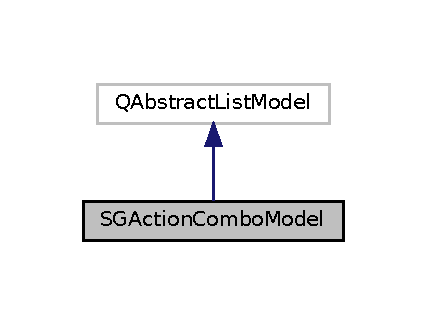
\includegraphics[width=205pt]{classSGActionComboModel__inherit__graph}
\end{center}
\end{figure}


Collaboration diagram for S\+G\+Action\+Combo\+Model\+:
\nopagebreak
\begin{figure}[H]
\begin{center}
\leavevmode
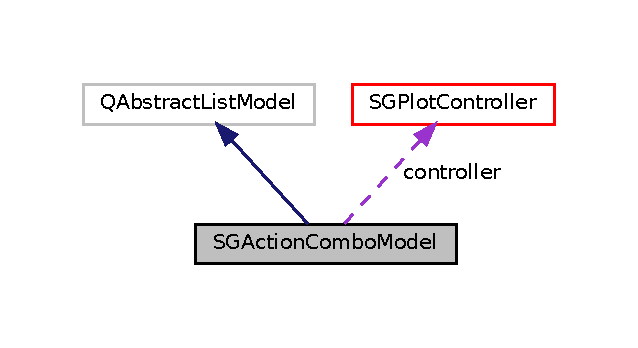
\includegraphics[width=306pt]{classSGActionComboModel__coll__graph}
\end{center}
\end{figure}
\subsection*{Public Slots}
\begin{DoxyCompactItemize}
\item 
\mbox{\Hypertarget{classSGActionComboModel_a66d596fb4ca91f5f4fe3f8d42ce12634}\label{classSGActionComboModel_a66d596fb4ca91f5f4fe3f8d42ce12634}} 
void \hyperlink{classSGActionComboModel_a66d596fb4ca91f5f4fe3f8d42ce12634}{action\+Changed} (int index)
\begin{DoxyCompactList}\small\item\em Signals to the associated action\+Controller to change the action. \end{DoxyCompactList}\item 
\mbox{\Hypertarget{classSGActionComboModel_a20046762e7cd9a5e3ceeadb382a04294}\label{classSGActionComboModel_a20046762e7cd9a5e3ceeadb382a04294}} 
void \hyperlink{classSGActionComboModel_a20046762e7cd9a5e3ceeadb382a04294}{change\+Layout} ()
\begin{DoxyCompactList}\small\item\em Signals to gui to change the layout. \end{DoxyCompactList}\end{DoxyCompactItemize}
\subsection*{Public Member Functions}
\begin{DoxyCompactItemize}
\item 
\mbox{\Hypertarget{classSGActionComboModel_a86bc33aa551e463e9b527b831cc95162}\label{classSGActionComboModel_a86bc33aa551e463e9b527b831cc95162}} 
\hyperlink{classSGActionComboModel_a86bc33aa551e463e9b527b831cc95162}{S\+G\+Action\+Combo\+Model} (\hyperlink{classSGPlotController}{S\+G\+Plot\+Controller} $\ast$\+\_\+controller)
\begin{DoxyCompactList}\small\item\em Constructor. \end{DoxyCompactList}\item 
\mbox{\Hypertarget{classSGActionComboModel_a6a070739e0bdbf37f72728b5b315dc7e}\label{classSGActionComboModel_a6a070739e0bdbf37f72728b5b315dc7e}} 
int \hyperlink{classSGActionComboModel_a6a070739e0bdbf37f72728b5b315dc7e}{row\+Count} (const Q\+Model\+Index \&parent) const
\begin{DoxyCompactList}\small\item\em Reimplement rowcount. \end{DoxyCompactList}\item 
\mbox{\Hypertarget{classSGActionComboModel_a40b862e251b8af402683a413fbe4aaf6}\label{classSGActionComboModel_a40b862e251b8af402683a413fbe4aaf6}} 
Q\+Variant \hyperlink{classSGActionComboModel_a40b862e251b8af402683a413fbe4aaf6}{data} (const Q\+Model\+Index \&index, int role) const
\begin{DoxyCompactList}\small\item\em Reimplement data. \end{DoxyCompactList}\end{DoxyCompactItemize}
\subsection*{Private Attributes}
\begin{DoxyCompactItemize}
\item 
\mbox{\Hypertarget{classSGActionComboModel_ab390b51f00169a101b370ebdb6cf5d5f}\label{classSGActionComboModel_ab390b51f00169a101b370ebdb6cf5d5f}} 
\hyperlink{classSGPlotController}{S\+G\+Plot\+Controller} $\ast$ \hyperlink{classSGActionComboModel_ab390b51f00169a101b370ebdb6cf5d5f}{controller}
\begin{DoxyCompactList}\small\item\em Pointer to the associated \hyperlink{classSGPlotController}{S\+G\+Plot\+Controller} object. \end{DoxyCompactList}\end{DoxyCompactItemize}


\subsection{Detailed Description}
Model for the action select menu. 

This class interfaces between the Q\+Combo\+Box for selecting the action and the underlying \hyperlink{classSGSolution}{S\+G\+Solution} object. The model automatically synchronizes the action\+Combo with the set of actions which are available on the current iteration and in the state selected in the state\+Combo, where the current iteration and state are controlled by the associated \hyperlink{classSGPlotController}{S\+G\+Plot\+Controller} object. When the action, state, or current\+Iter is changed in the \hyperlink{classSGPlotController}{S\+G\+Plot\+Controller}, the change\+Layout slot is triggered, which causes action\+Combo to request new data entries to reflect the actions that are available. The action that generates the best test direction is indicated with an asterisk. 

The documentation for this class was generated from the following file\+:\begin{DoxyCompactItemize}
\item 
viewer/hpp/sgactioncombomodel.\+hpp\end{DoxyCompactItemize}

\hypertarget{classSGActionComboModel__V2}{}\section{S\+G\+Action\+Combo\+Model\+\_\+\+V2 Class Reference}
\label{classSGActionComboModel__V2}\index{S\+G\+Action\+Combo\+Model\+\_\+\+V2@{S\+G\+Action\+Combo\+Model\+\_\+\+V2}}


Model for the action select menu.  




{\ttfamily \#include $<$sgactioncombomodel\+\_\+v2.\+hpp$>$}



Inheritance diagram for S\+G\+Action\+Combo\+Model\+\_\+\+V2\+:
\nopagebreak
\begin{figure}[H]
\begin{center}
\leavevmode
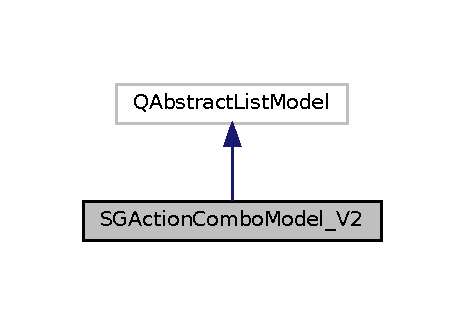
\includegraphics[width=223pt]{classSGActionComboModel__V2__inherit__graph}
\end{center}
\end{figure}


Collaboration diagram for S\+G\+Action\+Combo\+Model\+\_\+\+V2\+:
\nopagebreak
\begin{figure}[H]
\begin{center}
\leavevmode
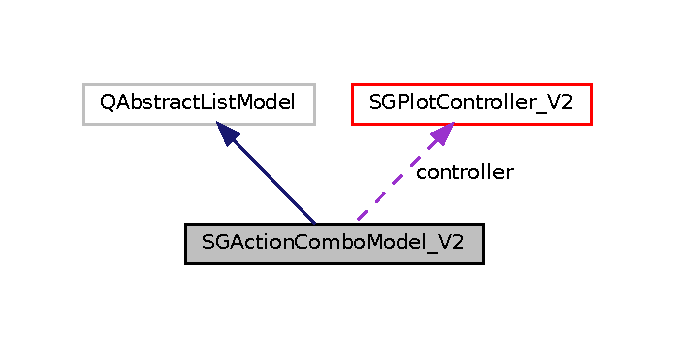
\includegraphics[width=324pt]{classSGActionComboModel__V2__coll__graph}
\end{center}
\end{figure}
\subsection*{Public Slots}
\begin{DoxyCompactItemize}
\item 
\mbox{\Hypertarget{classSGActionComboModel__V2_ad72d58c73cce1e08a710381ee991c7de}\label{classSGActionComboModel__V2_ad72d58c73cce1e08a710381ee991c7de}} 
void \hyperlink{classSGActionComboModel__V2_ad72d58c73cce1e08a710381ee991c7de}{action\+Changed} (int index)
\begin{DoxyCompactList}\small\item\em Signals to the associated action\+Controller to change the action. \end{DoxyCompactList}\item 
\mbox{\Hypertarget{classSGActionComboModel__V2_addfa2b818a357e947e018457d05af158}\label{classSGActionComboModel__V2_addfa2b818a357e947e018457d05af158}} 
void \hyperlink{classSGActionComboModel__V2_addfa2b818a357e947e018457d05af158}{change\+Layout} ()
\begin{DoxyCompactList}\small\item\em Signals to gui to change the layout. \end{DoxyCompactList}\end{DoxyCompactItemize}
\subsection*{Public Member Functions}
\begin{DoxyCompactItemize}
\item 
\mbox{\Hypertarget{classSGActionComboModel__V2_a4a6580cf7659a55e7e4e708d288bf87a}\label{classSGActionComboModel__V2_a4a6580cf7659a55e7e4e708d288bf87a}} 
\hyperlink{classSGActionComboModel__V2_a4a6580cf7659a55e7e4e708d288bf87a}{S\+G\+Action\+Combo\+Model\+\_\+\+V2} (\hyperlink{classSGPlotController__V2}{S\+G\+Plot\+Controller\+\_\+\+V2} $\ast$\+\_\+controller)
\begin{DoxyCompactList}\small\item\em Constructor. \end{DoxyCompactList}\item 
\mbox{\Hypertarget{classSGActionComboModel__V2_a4a46e78980cca2f225a9785496e5d3a2}\label{classSGActionComboModel__V2_a4a46e78980cca2f225a9785496e5d3a2}} 
int \hyperlink{classSGActionComboModel__V2_a4a46e78980cca2f225a9785496e5d3a2}{row\+Count} (const Q\+Model\+Index \&parent) const
\begin{DoxyCompactList}\small\item\em Reimplement rowcount. \end{DoxyCompactList}\item 
\mbox{\Hypertarget{classSGActionComboModel__V2_aeb624631b3be8b357a53abc6244ce761}\label{classSGActionComboModel__V2_aeb624631b3be8b357a53abc6244ce761}} 
Q\+Variant \hyperlink{classSGActionComboModel__V2_aeb624631b3be8b357a53abc6244ce761}{data} (const Q\+Model\+Index \&index, int role) const
\begin{DoxyCompactList}\small\item\em Reimplement data. \end{DoxyCompactList}\end{DoxyCompactItemize}
\subsection*{Private Attributes}
\begin{DoxyCompactItemize}
\item 
\mbox{\Hypertarget{classSGActionComboModel__V2_a66083a437effed4b59d09910bd556124}\label{classSGActionComboModel__V2_a66083a437effed4b59d09910bd556124}} 
\hyperlink{classSGPlotController__V2}{S\+G\+Plot\+Controller\+\_\+\+V2} $\ast$ \hyperlink{classSGActionComboModel__V2_a66083a437effed4b59d09910bd556124}{controller}
\begin{DoxyCompactList}\small\item\em Pointer to the associated \hyperlink{classSGPlotController__V2}{S\+G\+Plot\+Controller\+\_\+\+V2} object. \end{DoxyCompactList}\item 
\mbox{\Hypertarget{classSGActionComboModel__V2_a57557d54a151590564e8f229ae61ff2e}\label{classSGActionComboModel__V2_a57557d54a151590564e8f229ae61ff2e}} 
int {\bfseries state} = -\/1
\end{DoxyCompactItemize}


\subsection{Detailed Description}
Model for the action select menu. 

This class interfaces between the Q\+Combo\+Box for selecting the action and the underlying \hyperlink{classSGSolution}{S\+G\+Solution} object. The model automatically synchronizes the action\+Combo with the set of actions which are available on the current iteration and in the state selected in the state\+Combo, where the current iteration and state are controlled by the associated \hyperlink{classSGPlotController__V2}{S\+G\+Plot\+Controller\+\_\+\+V2} object. When the action, state, or current\+Iter is changed in the \hyperlink{classSGPlotController__V2}{S\+G\+Plot\+Controller\+\_\+\+V2}, the change\+Layout slot is triggered, which causes action\+Combo to request new data entries to reflect the actions that are available. The action that generates the best test direction is indicated with an asterisk. 

The documentation for this class was generated from the following files\+:\begin{DoxyCompactItemize}
\item 
viewer/hpp/sgactioncombomodel\+\_\+v2.\+hpp\item 
viewer/cpp/sgactioncombomodel\+\_\+v2.\+cpp\end{DoxyCompactItemize}

\hypertarget{classSGApprox}{\section{S\-G\-Approx Class Reference}
\label{classSGApprox}\index{S\-G\-Approx@{S\-G\-Approx}}
}


Approximation of the equilibrium payoff correspondence.  




{\ttfamily \#include $<$sgapprox.\-hpp$>$}

\subsection*{Public Member Functions}
\begin{DoxyCompactItemize}
\item 
\hypertarget{classSGApprox_a765c3c57b31d813ced0f7f93f6d4bb11}{\hyperlink{classSGApprox_a765c3c57b31d813ced0f7f93f6d4bb11}{S\-G\-Approx} (const \hyperlink{classSGEnv}{S\-G\-Env} \&\-\_\-env, const \hyperlink{classSGGame}{S\-G\-Game} \&\-\_\-game, \hyperlink{classSGSolution}{S\-G\-Solution} \&\-\_\-soln)}\label{classSGApprox_a765c3c57b31d813ced0f7f93f6d4bb11}

\begin{DoxyCompactList}\small\item\em Constructor for \hyperlink{classSGApprox}{S\-G\-Approx} class. \end{DoxyCompactList}\item 
void \hyperlink{classSGApprox_a4bca21d3b688b3ca283c6778c593563a}{initialize} ()
\begin{DoxyCompactList}\small\item\em Prepares the approximation for generation. \end{DoxyCompactList}\item 
double \hyperlink{classSGApprox_ac32645eb1ff336044f7ee5d523c610ce}{generate} ()
\begin{DoxyCompactList}\small\item\em Refines the approximation. \end{DoxyCompactList}\item 
\hypertarget{classSGApprox_a1099ea54bfba9b78417bec9b7f2751fc}{bool {\bfseries passed\-North} () const }\label{classSGApprox_a1099ea54bfba9b78417bec9b7f2751fc}

\item 
void \hyperlink{classSGApprox_af4ec568399b6e3ae16e6087d02381c12}{end} ()
\begin{DoxyCompactList}\small\item\em Destructor. \end{DoxyCompactList}\end{DoxyCompactItemize}
\subsection*{Private Member Functions}
\begin{DoxyCompactItemize}
\item 
void \hyperlink{classSGApprox_aea5ce8a2f48c7a572477f5f60520d565}{update\-Min\-Payoffs} ()
\begin{DoxyCompactList}\small\item\em Calculates the minimum I\-C continuation values. \end{DoxyCompactList}\item 
void \hyperlink{classSGApprox_a22804ad7335d810f6a48a304e618b4f2}{calculate\-Binding\-Continuations} ()
\begin{DoxyCompactList}\small\item\em Calculates binding continuation values. \end{DoxyCompactList}\item 
void \hyperlink{classSGApprox_abbd46d241613c871ecba24e10e115c56}{trim\-Binding\-Continuations} ()
\begin{DoxyCompactList}\small\item\em Trims binding continuation values. \end{DoxyCompactList}\item 
void \hyperlink{classSGApprox_a17d94998661d7d3fdb0618c8ce7dc53b}{find\-Best\-Direction} ()
\begin{DoxyCompactList}\small\item\em Calculates the best direction. \end{DoxyCompactList}\item 
void \hyperlink{classSGApprox_ad545fa06b93fd2241c798cf8661cc092}{calculate\-New\-Pivot} ()
\begin{DoxyCompactList}\small\item\em Calculates the new pivot. \end{DoxyCompactList}\item 
double \hyperlink{classSGApprox_aa893563e95936ed12a3e3b4e1ba7ac54}{update\-Pivot} (vector$<$ double $>$ \&movements, vector$<$ double $>$ \&changes, vector$<$ bool $>$ \&\hyperlink{classSGApprox_ac05d3697e39d0f671858fd9936581820}{non\-Binding\-States}, const vector$<$ double $>$ \&max\-Movement)
\begin{DoxyCompactList}\small\item\em Updates the pivot. \end{DoxyCompactList}\item 
void \hyperlink{classSGApprox_a93455458a21bdeccff21a6163932c38a}{update\-Flags} ()
\begin{DoxyCompactList}\small\item\em Updates flags before the next iteration. \end{DoxyCompactList}\item 
double \hyperlink{classSGApprox_a78d8cbb1e3727aef21d4666164a21207}{distance} (int new\-Start, int start, int old\-Start) const 
\begin{DoxyCompactList}\small\item\em Calculates the distance between revolutions. \end{DoxyCompactList}\item 
bool \hyperlink{classSGApprox_aa251718a9291407cc4e758253c6d29ea}{improves} (const \hyperlink{classSGPoint}{S\-G\-Point} \&current, const \hyperlink{classSGPoint}{S\-G\-Point} \&best, const \hyperlink{classSGPoint}{S\-G\-Point} \&new\-Direction) const 
\begin{DoxyCompactList}\small\item\em Checks whether or not new\-Direction is shallower than best, relative to current. \end{DoxyCompactList}\item 
\hypertarget{classSGApprox_a91be640b991ff44b56359cbe3a2b00d5}{void \hyperlink{classSGApprox_a91be640b991ff44b56359cbe3a2b00d5}{log\-Append} (ofstream \&\hyperlink{classSGApprox_aa95ff6bda46617fbaa7cf1c8d6708748}{logfs}, int iter, int rev, const \hyperlink{classSGTuple}{S\-G\-Tuple} \&tuple, int state, int action)}\label{classSGApprox_a91be640b991ff44b56359cbe3a2b00d5}

\begin{DoxyCompactList}\small\item\em Outputs progress to the log file every iteration. \end{DoxyCompactList}\item 
\hypertarget{classSGApprox_a55e023f8f5c0c6cf906999c0682d6765}{std\-::string \hyperlink{classSGApprox_a55e023f8f5c0c6cf906999c0682d6765}{progress\-String} () const }\label{classSGApprox_a55e023f8f5c0c6cf906999c0682d6765}

\begin{DoxyCompactList}\small\item\em Returns a string indicating the algorithms progress. \end{DoxyCompactList}\end{DoxyCompactItemize}
\subsection*{Private Attributes}
\begin{DoxyCompactItemize}
\item 
const \hyperlink{classSGEnv}{S\-G\-Env} \& \hyperlink{classSGApprox_a6597417918c1e6c764f4f943c72af781}{env}
\item 
const \hyperlink{classSGGame}{S\-G\-Game} \& \hyperlink{classSGApprox_a0774e3ed0ff009809606a42c9e7ef727}{game}
\item 
\hyperlink{classSGSolution}{S\-G\-Solution} \& \hyperlink{classSGApprox_aaed7d16ba723bbdfbec94b21e0edff8e}{soln}
\item 
const double \hyperlink{classSGApprox_ad105b178e4e85845ce5a85e26d7d038b}{delta}
\item 
const int \hyperlink{classSGApprox_a6f512c1cb974247ecb24c2201f045905}{num\-Players}
\item 
const int \hyperlink{classSGApprox_a676bda37d610e501eac72037d22b5293}{num\-States}
\item 
const vector$<$ vector$<$ int $>$ $>$ \& \hyperlink{classSGApprox_af3208841348d868b372549dd7508e300}{num\-Actions}
\item 
const vector$<$ int $>$ \& \hyperlink{classSGApprox_a0b3cacf6c192238c0fa753c4d71358c6}{num\-Actions\-\_\-total}
\item 
const vector$<$ vector$<$ \hyperlink{classSGPoint}{S\-G\-Point} $>$ $>$ \& \hyperlink{classSGApprox_a053be8812a4cba4f529379dbfab0c5aa}{payoffs}
\item 
const vector$<$ vector$<$ vector\\*
$<$ double $>$ $>$ $>$ \& \hyperlink{classSGApprox_aaedd93c6e7faddcf4f33fceec383c562}{probabilities}
\item 
const vector$<$ list$<$ int $>$ $>$ \& \hyperlink{classSGApprox_ac737ccb3686428f766d9b69008dc897e}{eq\-Actions}
\item 
const vector$<$ bool $>$ \& \hyperlink{classSGApprox_a302549fb3037b3db0e6313db35229c97}{unconstrained}
\item 
std\-::ofstream \hyperlink{classSGApprox_aa95ff6bda46617fbaa7cf1c8d6708748}{logfs}
\item 
int \hyperlink{classSGApprox_a7ab53424f5933726a15001ff2885a4a9}{num\-Iterations}
\item 
int \hyperlink{classSGApprox_a2bd0cab80a3f8d799fdc2841b65dd2c2}{num\-Revolutions}
\item 
double \hyperlink{classSGApprox_aee816ed49535cfc211aa34d0e6064e01}{error\-Level}
\item 
vector$<$ bool $>$ \hyperlink{classSGApprox_a44ce2e0eba77e1c7c155f38662cba9d0}{facing\-East\-North}
\item 
bool \hyperlink{classSGApprox_aec0377b26f0efaea314f72554a8862b9}{pass\-North}
\item 
vector$<$ bool $>$ \hyperlink{classSGApprox_ae680fd19d6a65aecee81dffeba8e8595}{updated\-Threat\-Tuple}
\item 
vector$<$ list$<$ \hyperlink{classSGAction}{S\-G\-Action} $>$ $>$ \hyperlink{classSGApprox_a0fccecf0f5dbe7e9288e47182f180879}{actions}
\item 
vector$<$ \hyperlink{classSGTuple}{S\-G\-Tuple} $>$ \hyperlink{classSGApprox_ab0e2c4678401f806922ac64667ad5ff6}{extreme\-Tuples}
\item 
\hyperlink{classSGTuple}{S\-G\-Tuple} \hyperlink{classSGApprox_a69815072fd57ec5b6b137dc839371ec7}{threat\-Tuple}
\item 
\hyperlink{classSGTuple}{S\-G\-Tuple} \hyperlink{classSGApprox_a037c73ff2b6ff8a55fadf57bb0a6a546}{pivot}
\item 
\hyperlink{classSGPoint}{S\-G\-Point} \hyperlink{classSGApprox_ac5bf5f2eba2d65c8a9933b6d74f0cd47}{current\-Direction}
\item 
vector$<$ const \hyperlink{classSGAction}{S\-G\-Action} $\ast$ $>$ \hyperlink{classSGApprox_a507eb6895c5a99c5d1efba8107989187}{action\-Tuple}
\item 
vector$<$ bool $>$ \hyperlink{classSGApprox_ac05d3697e39d0f671858fd9936581820}{non\-Binding\-States}
\item 
const \hyperlink{classSGAction}{S\-G\-Action} $\ast$ \hyperlink{classSGApprox_a9769774aa8829e1e5adec2e4a2bb35ae}{best\-Action}
\item 
\hyperlink{classSGPoint}{S\-G\-Point} \hyperlink{classSGApprox_a20454173d5c9af9bd24870d97f4e2b91}{best\-Direction}
\item 
bool \hyperlink{classSGApprox_ac1a670470711fd81c00aba76d8213ade}{best\-Not\-Binding}
\item 
int \hyperlink{classSGApprox_aa0c6296f28ce5527edc9829e4d9c23a1}{west\-Point}
\item 
int \hyperlink{classSGApprox_aed002d6e06e7199e10b3ac4f27b6cb6c}{new\-West}
\item 
\hypertarget{classSGApprox_a130b9dc6e354a70a0f3cf08c5a511c99}{int {\bfseries old\-West}}\label{classSGApprox_a130b9dc6e354a70a0f3cf08c5a511c99}

\end{DoxyCompactItemize}
\subsection*{Friends}
\begin{DoxyCompactItemize}
\item 
\hypertarget{classSGApprox_a8b0e5d2bebfed7e7e032366bb49bc5f1}{class {\bfseries S\-G\-Solver}}\label{classSGApprox_a8b0e5d2bebfed7e7e032366bb49bc5f1}

\item 
\hypertarget{classSGApprox_a57e09eb109cadcde666335f9e8af571a}{class {\bfseries S\-G\-Main\-Window}}\label{classSGApprox_a57e09eb109cadcde666335f9e8af571a}

\item 
\hypertarget{classSGApprox_a0738b92f2a44c43a342e41240c0f733c}{class {\bfseries S\-G\-Solver\-Worker}}\label{classSGApprox_a0738b92f2a44c43a342e41240c0f733c}

\end{DoxyCompactItemize}


\subsection{Detailed Description}
Approximation of the equilibrium payoff correspondence. 

This class contains an approximation of the equilibrium payoff correspondence. At its core, it contains a sequence of extreme tuples that have been generated thus far, a pivot, and a direction. The main method, \hyperlink{classSGApprox_ac32645eb1ff336044f7ee5d523c610ce}{S\-G\-Approx\-::generate()}, finds a new direction that will not intersect the equilibrium payoff correspondence and updates the pivot in that direction. By successively calling \hyperlink{classSGApprox_ac32645eb1ff336044f7ee5d523c610ce}{S\-G\-Approx\-::generate()}, the approximation will be refined and asymptotically it will converge to the equilibrium payoff correspondence. 

\subsection{Member Function Documentation}
\hypertarget{classSGApprox_a22804ad7335d810f6a48a304e618b4f2}{\index{S\-G\-Approx@{S\-G\-Approx}!calculate\-Binding\-Continuations@{calculate\-Binding\-Continuations}}
\index{calculate\-Binding\-Continuations@{calculate\-Binding\-Continuations}!SGApprox@{S\-G\-Approx}}
\subsubsection[{calculate\-Binding\-Continuations}]{\setlength{\rightskip}{0pt plus 5cm}void S\-G\-Approx\-::calculate\-Binding\-Continuations (
\begin{DoxyParamCaption}
{}
\end{DoxyParamCaption}
)\hspace{0.3cm}{\ttfamily [private]}}}\label{classSGApprox_a22804ad7335d810f6a48a304e618b4f2}


Calculates binding continuation values. 

For each \hyperlink{classSGAction}{S\-G\-Action} objection in \hyperlink{classSGApprox_a0fccecf0f5dbe7e9288e47182f180879}{S\-G\-Approx\-::actions}, this method computes the extreme binding continuation values relative to the current threat tuple and the trajectory of the pivot on the previous revolution. \hypertarget{classSGApprox_ad545fa06b93fd2241c798cf8661cc092}{\index{S\-G\-Approx@{S\-G\-Approx}!calculate\-New\-Pivot@{calculate\-New\-Pivot}}
\index{calculate\-New\-Pivot@{calculate\-New\-Pivot}!SGApprox@{S\-G\-Approx}}
\subsubsection[{calculate\-New\-Pivot}]{\setlength{\rightskip}{0pt plus 5cm}void S\-G\-Approx\-::calculate\-New\-Pivot (
\begin{DoxyParamCaption}
{}
\end{DoxyParamCaption}
)\hspace{0.3cm}{\ttfamily [private]}}}\label{classSGApprox_ad545fa06b93fd2241c798cf8661cc092}


Calculates the new pivot. 

After the best direction has been found, this method updates the pivot in the new current direction. First, it calculates the maximum movements in the current direction that would not violate incentive compatibility, and then iterates \hyperlink{classSGApprox_aa893563e95936ed12a3e3b4e1ba7ac54}{S\-G\-Approx\-::update\-Pivot} until the pivot converges. \hypertarget{classSGApprox_a78d8cbb1e3727aef21d4666164a21207}{\index{S\-G\-Approx@{S\-G\-Approx}!distance@{distance}}
\index{distance@{distance}!SGApprox@{S\-G\-Approx}}
\subsubsection[{distance}]{\setlength{\rightskip}{0pt plus 5cm}double S\-G\-Approx\-::distance (
\begin{DoxyParamCaption}
\item[{int}]{new\-Start, }
\item[{int}]{start, }
\item[{int}]{old\-Start}
\end{DoxyParamCaption}
) const\hspace{0.3cm}{\ttfamily [private]}}}\label{classSGApprox_a78d8cbb1e3727aef21d4666164a21207}


Calculates the distance between revolutions. 

Returns the distance between successive iterations. Only runs when \hyperlink{classSGApprox_aec0377b26f0efaea314f72554a8862b9}{S\-G\-Approx\-::pass\-North} is true. Currently only runs when the number of \hyperlink{classSGTuple}{S\-G\-Tuple} objects on successive revolutions is the same, and then takes the maximum over all distances between tuples that are in corresponding positions in the revolutions. \hypertarget{classSGApprox_af4ec568399b6e3ae16e6087d02381c12}{\index{S\-G\-Approx@{S\-G\-Approx}!end@{end}}
\index{end@{end}!SGApprox@{S\-G\-Approx}}
\subsubsection[{end}]{\setlength{\rightskip}{0pt plus 5cm}void S\-G\-Approx\-::end (
\begin{DoxyParamCaption}
{}
\end{DoxyParamCaption}
)}}\label{classSGApprox_af4ec568399b6e3ae16e6087d02381c12}


Destructor. 

Only purpose right now is to close the log file. \hypertarget{classSGApprox_a17d94998661d7d3fdb0618c8ce7dc53b}{\index{S\-G\-Approx@{S\-G\-Approx}!find\-Best\-Direction@{find\-Best\-Direction}}
\index{find\-Best\-Direction@{find\-Best\-Direction}!SGApprox@{S\-G\-Approx}}
\subsubsection[{find\-Best\-Direction}]{\setlength{\rightskip}{0pt plus 5cm}void S\-G\-Approx\-::find\-Best\-Direction (
\begin{DoxyParamCaption}
{}
\end{DoxyParamCaption}
)\hspace{0.3cm}{\ttfamily [private]}}}\label{classSGApprox_a17d94998661d7d3fdb0618c8ce7dc53b}


Calculates the best direction. 

Iteraties over the \hyperlink{classSGAction}{S\-G\-Action} objects in \hyperlink{classSGApprox_a0fccecf0f5dbe7e9288e47182f180879}{S\-G\-Approx\-::actions} to find the shallowest admissible direction, and stores it in best\-Direction. \hypertarget{classSGApprox_ac32645eb1ff336044f7ee5d523c610ce}{\index{S\-G\-Approx@{S\-G\-Approx}!generate@{generate}}
\index{generate@{generate}!SGApprox@{S\-G\-Approx}}
\subsubsection[{generate}]{\setlength{\rightskip}{0pt plus 5cm}double S\-G\-Approx\-::generate (
\begin{DoxyParamCaption}
{}
\end{DoxyParamCaption}
)}}\label{classSGApprox_ac32645eb1ff336044f7ee5d523c610ce}


Refines the approximation. 

Main public routine for the \hyperlink{classSGApprox}{S\-G\-Approx} class. Updates minimum I\-C continuation values and binding continuation values, finds the best new direction, advances the pivot, and resets the flags. Also returns the distance between revolutions when a revolution is completed. Otherwise, returns 1. \hypertarget{classSGApprox_aa251718a9291407cc4e758253c6d29ea}{\index{S\-G\-Approx@{S\-G\-Approx}!improves@{improves}}
\index{improves@{improves}!SGApprox@{S\-G\-Approx}}
\subsubsection[{improves}]{\setlength{\rightskip}{0pt plus 5cm}bool S\-G\-Approx\-::improves (
\begin{DoxyParamCaption}
\item[{const {\bf S\-G\-Point} \&}]{current, }
\item[{const {\bf S\-G\-Point} \&}]{best, }
\item[{const {\bf S\-G\-Point} \&}]{new\-Direction}
\end{DoxyParamCaption}
) const\hspace{0.3cm}{\ttfamily [private]}}}\label{classSGApprox_aa251718a9291407cc4e758253c6d29ea}


Checks whether or not new\-Direction is shallower than best, relative to current. 

Returns true if the cosine between new\-Direction and best is greater than \hyperlink{classSGEnv_af5c8453c8d759ea826b066b22bfa73fd}{S\-G\-Env\-::improve\-Tol}, or if best and new\-Direction are colinear, whether or not best has a larger norm. Non-\/static so it can read the parameter values in \hyperlink{classSGApprox_a6597417918c1e6c764f4f943c72af781}{S\-G\-Approx\-::env}. \hypertarget{classSGApprox_a4bca21d3b688b3ca283c6778c593563a}{\index{S\-G\-Approx@{S\-G\-Approx}!initialize@{initialize}}
\index{initialize@{initialize}!SGApprox@{S\-G\-Approx}}
\subsubsection[{initialize}]{\setlength{\rightskip}{0pt plus 5cm}void S\-G\-Approx\-::initialize (
\begin{DoxyParamCaption}
{}
\end{DoxyParamCaption}
)}}\label{classSGApprox_a4bca21d3b688b3ca283c6778c593563a}


Prepares the approximation for generation. 

Opens the log file, constructs the actions array, initializes extreme\-Tuples to a large \char`\"{}box\char`\"{} correspondence that contains the equilibrium payoff correspondence. Also initializes the pivot and the first direction. Sets the flags so that \hyperlink{classSGApprox_ac32645eb1ff336044f7ee5d523c610ce}{S\-G\-Approx\-::generate()} will calculate new binding continuation values on the first pass. \hypertarget{classSGApprox_abbd46d241613c871ecba24e10e115c56}{\index{S\-G\-Approx@{S\-G\-Approx}!trim\-Binding\-Continuations@{trim\-Binding\-Continuations}}
\index{trim\-Binding\-Continuations@{trim\-Binding\-Continuations}!SGApprox@{S\-G\-Approx}}
\subsubsection[{trim\-Binding\-Continuations}]{\setlength{\rightskip}{0pt plus 5cm}void S\-G\-Approx\-::trim\-Binding\-Continuations (
\begin{DoxyParamCaption}
{}
\end{DoxyParamCaption}
)\hspace{0.3cm}{\ttfamily [private]}}}\label{classSGApprox_abbd46d241613c871ecba24e10e115c56}


Trims binding continuation values. 

For each \hyperlink{classSGAction}{S\-G\-Action} in \hyperlink{classSGApprox_a0fccecf0f5dbe7e9288e47182f180879}{S\-G\-Approx\-::actions}, this method \char`\"{}trims\char`\"{} the binding payoff segents by intersecting them with the half-\/space correspondence that is below the pivot in the direction normal to the current direction. Not currently being used. \hypertarget{classSGApprox_a93455458a21bdeccff21a6163932c38a}{\index{S\-G\-Approx@{S\-G\-Approx}!update\-Flags@{update\-Flags}}
\index{update\-Flags@{update\-Flags}!SGApprox@{S\-G\-Approx}}
\subsubsection[{update\-Flags}]{\setlength{\rightskip}{0pt plus 5cm}void S\-G\-Approx\-::update\-Flags (
\begin{DoxyParamCaption}
{}
\end{DoxyParamCaption}
)\hspace{0.3cm}{\ttfamily [private]}}}\label{classSGApprox_a93455458a21bdeccff21a6163932c38a}


Updates flags before the next iteration. 

This method checks whether or not the threat tuple has increased and sets the flags for recalculating binding continuation values. Also checks whether or not the cardinal direction has changed, and updates \hyperlink{classSGApprox_a44ce2e0eba77e1c7c155f38662cba9d0}{S\-G\-Approx\-::facing\-East\-North} and \hyperlink{classSGApprox_aec0377b26f0efaea314f72554a8862b9}{S\-G\-Approx\-::pass\-North}. \hypertarget{classSGApprox_aea5ce8a2f48c7a572477f5f60520d565}{\index{S\-G\-Approx@{S\-G\-Approx}!update\-Min\-Payoffs@{update\-Min\-Payoffs}}
\index{update\-Min\-Payoffs@{update\-Min\-Payoffs}!SGApprox@{S\-G\-Approx}}
\subsubsection[{update\-Min\-Payoffs}]{\setlength{\rightskip}{0pt plus 5cm}void S\-G\-Approx\-::update\-Min\-Payoffs (
\begin{DoxyParamCaption}
{}
\end{DoxyParamCaption}
)\hspace{0.3cm}{\ttfamily [private]}}}\label{classSGApprox_aea5ce8a2f48c7a572477f5f60520d565}


Calculates the minimum I\-C continuation values. 

This method calculates for each \hyperlink{classSGAction}{S\-G\-Action} object in \hyperlink{classSGApprox_a0fccecf0f5dbe7e9288e47182f180879}{S\-G\-Approx\-::actions} the minimum incentive compatible continuation value, relative to the current threat tuple. \hypertarget{classSGApprox_aa893563e95936ed12a3e3b4e1ba7ac54}{\index{S\-G\-Approx@{S\-G\-Approx}!update\-Pivot@{update\-Pivot}}
\index{update\-Pivot@{update\-Pivot}!SGApprox@{S\-G\-Approx}}
\subsubsection[{update\-Pivot}]{\setlength{\rightskip}{0pt plus 5cm}double S\-G\-Approx\-::update\-Pivot (
\begin{DoxyParamCaption}
\item[{vector$<$ double $>$ \&}]{movements, }
\item[{vector$<$ double $>$ \&}]{changes, }
\item[{vector$<$ bool $>$ \&}]{non\-Binding\-States, }
\item[{const vector$<$ double $>$ \&}]{max\-Movement}
\end{DoxyParamCaption}
)\hspace{0.3cm}{\ttfamily [private]}}}\label{classSGApprox_aa893563e95936ed12a3e3b4e1ba7ac54}


Updates the pivot. 

Bellman operator that advances the pivots corresponding to non-\/binding states in the current direction. If an I\-C constraint would be violated in state s, the movement in state s is set to max\-Movement\mbox{[}s\mbox{]} and the state is put into the binding regime. Returns the distance the pivot moves. 

\subsection{Member Data Documentation}
\hypertarget{classSGApprox_a0fccecf0f5dbe7e9288e47182f180879}{\index{S\-G\-Approx@{S\-G\-Approx}!actions@{actions}}
\index{actions@{actions}!SGApprox@{S\-G\-Approx}}
\subsubsection[{actions}]{\setlength{\rightskip}{0pt plus 5cm}vector$<$ list$<${\bf S\-G\-Action}$>$ $>$ S\-G\-Approx\-::actions\hspace{0.3cm}{\ttfamily [private]}}}\label{classSGApprox_a0fccecf0f5dbe7e9288e47182f180879}
actions\mbox{[}state\mbox{]} is a list of actions that can still be supported according to the current approximation. \hypertarget{classSGApprox_a507eb6895c5a99c5d1efba8107989187}{\index{S\-G\-Approx@{S\-G\-Approx}!action\-Tuple@{action\-Tuple}}
\index{action\-Tuple@{action\-Tuple}!SGApprox@{S\-G\-Approx}}
\subsubsection[{action\-Tuple}]{\setlength{\rightskip}{0pt plus 5cm}vector$<$ const {\bf S\-G\-Action}$\ast$ $>$ S\-G\-Approx\-::action\-Tuple\hspace{0.3cm}{\ttfamily [private]}}}\label{classSGApprox_a507eb6895c5a99c5d1efba8107989187}
action\-Tuple\mbox{[}state\mbox{]} is a pointer to the \hyperlink{classSGAction}{S\-G\-Action} object that generates pivot\mbox{[}state\mbox{]}. \hypertarget{classSGApprox_a9769774aa8829e1e5adec2e4a2bb35ae}{\index{S\-G\-Approx@{S\-G\-Approx}!best\-Action@{best\-Action}}
\index{best\-Action@{best\-Action}!SGApprox@{S\-G\-Approx}}
\subsubsection[{best\-Action}]{\setlength{\rightskip}{0pt plus 5cm}const {\bf S\-G\-Action}$\ast$ S\-G\-Approx\-::best\-Action\hspace{0.3cm}{\ttfamily [private]}}}\label{classSGApprox_a9769774aa8829e1e5adec2e4a2bb35ae}
Pointer to the action profile that generates the shallowest direction. \hypertarget{classSGApprox_a20454173d5c9af9bd24870d97f4e2b91}{\index{S\-G\-Approx@{S\-G\-Approx}!best\-Direction@{best\-Direction}}
\index{best\-Direction@{best\-Direction}!SGApprox@{S\-G\-Approx}}
\subsubsection[{best\-Direction}]{\setlength{\rightskip}{0pt plus 5cm}{\bf S\-G\-Point} S\-G\-Approx\-::best\-Direction\hspace{0.3cm}{\ttfamily [private]}}}\label{classSGApprox_a20454173d5c9af9bd24870d97f4e2b91}
The shallowest direction at the current iteration. \hypertarget{classSGApprox_ac1a670470711fd81c00aba76d8213ade}{\index{S\-G\-Approx@{S\-G\-Approx}!best\-Not\-Binding@{best\-Not\-Binding}}
\index{best\-Not\-Binding@{best\-Not\-Binding}!SGApprox@{S\-G\-Approx}}
\subsubsection[{best\-Not\-Binding}]{\setlength{\rightskip}{0pt plus 5cm}bool S\-G\-Approx\-::best\-Not\-Binding\hspace{0.3cm}{\ttfamily [private]}}}\label{classSGApprox_ac1a670470711fd81c00aba76d8213ade}
True if the shallowest direction was generated with the non-\/binding regime. \hypertarget{classSGApprox_ac5bf5f2eba2d65c8a9933b6d74f0cd47}{\index{S\-G\-Approx@{S\-G\-Approx}!current\-Direction@{current\-Direction}}
\index{current\-Direction@{current\-Direction}!SGApprox@{S\-G\-Approx}}
\subsubsection[{current\-Direction}]{\setlength{\rightskip}{0pt plus 5cm}{\bf S\-G\-Point} S\-G\-Approx\-::current\-Direction\hspace{0.3cm}{\ttfamily [private]}}}\label{classSGApprox_ac5bf5f2eba2d65c8a9933b6d74f0cd47}
The current direction. \hypertarget{classSGApprox_ad105b178e4e85845ce5a85e26d7d038b}{\index{S\-G\-Approx@{S\-G\-Approx}!delta@{delta}}
\index{delta@{delta}!SGApprox@{S\-G\-Approx}}
\subsubsection[{delta}]{\setlength{\rightskip}{0pt plus 5cm}const double S\-G\-Approx\-::delta\hspace{0.3cm}{\ttfamily [private]}}}\label{classSGApprox_ad105b178e4e85845ce5a85e26d7d038b}
The discount factor, copied from \hyperlink{classSGApprox_a0774e3ed0ff009809606a42c9e7ef727}{S\-G\-Approx\-::game}. \hypertarget{classSGApprox_a6597417918c1e6c764f4f943c72af781}{\index{S\-G\-Approx@{S\-G\-Approx}!env@{env}}
\index{env@{env}!SGApprox@{S\-G\-Approx}}
\subsubsection[{env}]{\setlength{\rightskip}{0pt plus 5cm}const {\bf S\-G\-Env}\& S\-G\-Approx\-::env\hspace{0.3cm}{\ttfamily [private]}}}\label{classSGApprox_a6597417918c1e6c764f4f943c72af781}
Constant reference to the parent environment. \hypertarget{classSGApprox_ac737ccb3686428f766d9b69008dc897e}{\index{S\-G\-Approx@{S\-G\-Approx}!eq\-Actions@{eq\-Actions}}
\index{eq\-Actions@{eq\-Actions}!SGApprox@{S\-G\-Approx}}
\subsubsection[{eq\-Actions}]{\setlength{\rightskip}{0pt plus 5cm}const vector$<$ list$<$int$>$ $>$\& S\-G\-Approx\-::eq\-Actions\hspace{0.3cm}{\ttfamily [private]}}}\label{classSGApprox_ac737ccb3686428f766d9b69008dc897e}
\begin{DoxyVerb}     List of action profiles
\end{DoxyVerb}
 that are allowed in equilibrium. Const reference to \hyperlink{classSGGame_a900ba2e4035c19b19dd5342219862347}{S\-G\-Game\-::eq\-Actions} in \hyperlink{classSGApprox_a0774e3ed0ff009809606a42c9e7ef727}{S\-G\-Approx\-::game}. \hypertarget{classSGApprox_aee816ed49535cfc211aa34d0e6064e01}{\index{S\-G\-Approx@{S\-G\-Approx}!error\-Level@{error\-Level}}
\index{error\-Level@{error\-Level}!SGApprox@{S\-G\-Approx}}
\subsubsection[{error\-Level}]{\setlength{\rightskip}{0pt plus 5cm}double S\-G\-Approx\-::error\-Level\hspace{0.3cm}{\ttfamily [private]}}}\label{classSGApprox_aee816ed49535cfc211aa34d0e6064e01}
Current error level \hypertarget{classSGApprox_ab0e2c4678401f806922ac64667ad5ff6}{\index{S\-G\-Approx@{S\-G\-Approx}!extreme\-Tuples@{extreme\-Tuples}}
\index{extreme\-Tuples@{extreme\-Tuples}!SGApprox@{S\-G\-Approx}}
\subsubsection[{extreme\-Tuples}]{\setlength{\rightskip}{0pt plus 5cm}vector$<${\bf S\-G\-Tuple}$>$ S\-G\-Approx\-::extreme\-Tuples\hspace{0.3cm}{\ttfamily [private]}}}\label{classSGApprox_ab0e2c4678401f806922ac64667ad5ff6}
Past trajectory of the pivot. \hypertarget{classSGApprox_a44ce2e0eba77e1c7c155f38662cba9d0}{\index{S\-G\-Approx@{S\-G\-Approx}!facing\-East\-North@{facing\-East\-North}}
\index{facing\-East\-North@{facing\-East\-North}!SGApprox@{S\-G\-Approx}}
\subsubsection[{facing\-East\-North}]{\setlength{\rightskip}{0pt plus 5cm}vector$<$bool$>$ S\-G\-Approx\-::facing\-East\-North\hspace{0.3cm}{\ttfamily [private]}}}\label{classSGApprox_a44ce2e0eba77e1c7c155f38662cba9d0}
Indicates whether the current direction points east (if facing\-East\-North\mbox{[}0\mbox{]}=true) and north (if facing\-East\-North\mbox{[}1\mbox{]}=true). \hypertarget{classSGApprox_a0774e3ed0ff009809606a42c9e7ef727}{\index{S\-G\-Approx@{S\-G\-Approx}!game@{game}}
\index{game@{game}!SGApprox@{S\-G\-Approx}}
\subsubsection[{game}]{\setlength{\rightskip}{0pt plus 5cm}const {\bf S\-G\-Game}\& S\-G\-Approx\-::game\hspace{0.3cm}{\ttfamily [private]}}}\label{classSGApprox_a0774e3ed0ff009809606a42c9e7ef727}
Constant reference to the game being solved. \hypertarget{classSGApprox_aa95ff6bda46617fbaa7cf1c8d6708748}{\index{S\-G\-Approx@{S\-G\-Approx}!logfs@{logfs}}
\index{logfs@{logfs}!SGApprox@{S\-G\-Approx}}
\subsubsection[{logfs}]{\setlength{\rightskip}{0pt plus 5cm}std\-::ofstream S\-G\-Approx\-::logfs\hspace{0.3cm}{\ttfamily [private]}}}\label{classSGApprox_aa95ff6bda46617fbaa7cf1c8d6708748}
File stream for log file. \hypertarget{classSGApprox_aed002d6e06e7199e10b3ac4f27b6cb6c}{\index{S\-G\-Approx@{S\-G\-Approx}!new\-West@{new\-West}}
\index{new\-West@{new\-West}!SGApprox@{S\-G\-Approx}}
\subsubsection[{new\-West}]{\setlength{\rightskip}{0pt plus 5cm}int S\-G\-Approx\-::new\-West\hspace{0.3cm}{\ttfamily [private]}}}\label{classSGApprox_aed002d6e06e7199e10b3ac4f27b6cb6c}
\begin{DoxyVerb}       Index within SGApprox::extremeTuples of the
\end{DoxyVerb}
 westernmost tuple on the current revolution. \hypertarget{classSGApprox_ac05d3697e39d0f671858fd9936581820}{\index{S\-G\-Approx@{S\-G\-Approx}!non\-Binding\-States@{non\-Binding\-States}}
\index{non\-Binding\-States@{non\-Binding\-States}!SGApprox@{S\-G\-Approx}}
\subsubsection[{non\-Binding\-States}]{\setlength{\rightskip}{0pt plus 5cm}vector$<$bool$>$ S\-G\-Approx\-::non\-Binding\-States\hspace{0.3cm}{\ttfamily [private]}}}\label{classSGApprox_ac05d3697e39d0f671858fd9936581820}
non\-Binding\-States\mbox{[}state\mbox{]}=true if pivot\mbox{[}state\mbox{]} was generated in the non-\/binding regime. \hypertarget{classSGApprox_af3208841348d868b372549dd7508e300}{\index{S\-G\-Approx@{S\-G\-Approx}!num\-Actions@{num\-Actions}}
\index{num\-Actions@{num\-Actions}!SGApprox@{S\-G\-Approx}}
\subsubsection[{num\-Actions}]{\setlength{\rightskip}{0pt plus 5cm}const vector$<$ vector$<$int$>$ $>$\& S\-G\-Approx\-::num\-Actions\hspace{0.3cm}{\ttfamily [private]}}}\label{classSGApprox_af3208841348d868b372549dd7508e300}
Player i in state s has num\-Actions\mbox{[}s\mbox{]}\mbox{[}i\mbox{]} actions. Constant reference to \hyperlink{classSGGame_acebe94d195ffb67f92925bcd4c26d1a9}{S\-G\-Game\-::num\-Actions} in \hyperlink{classSGApprox_a0774e3ed0ff009809606a42c9e7ef727}{S\-G\-Approx\-::game}. \hypertarget{classSGApprox_a0b3cacf6c192238c0fa753c4d71358c6}{\index{S\-G\-Approx@{S\-G\-Approx}!num\-Actions\-\_\-total@{num\-Actions\-\_\-total}}
\index{num\-Actions\-\_\-total@{num\-Actions\-\_\-total}!SGApprox@{S\-G\-Approx}}
\subsubsection[{num\-Actions\-\_\-total}]{\setlength{\rightskip}{0pt plus 5cm}const vector$<$int$>$\& S\-G\-Approx\-::num\-Actions\-\_\-total\hspace{0.3cm}{\ttfamily [private]}}}\label{classSGApprox_a0b3cacf6c192238c0fa753c4d71358c6}
In state s, there are a total of num\-Actions\-\_\-total\mbox{[}s\mbox{]} action profiles. Constant reference to \hyperlink{classSGGame_a3b219a37177b5b8b38737f570e419429}{S\-G\-Game\-::num\-Actions\-\_\-total} in \hyperlink{classSGApprox_a0774e3ed0ff009809606a42c9e7ef727}{S\-G\-Approx\-::game}. \hypertarget{classSGApprox_a7ab53424f5933726a15001ff2885a4a9}{\index{S\-G\-Approx@{S\-G\-Approx}!num\-Iterations@{num\-Iterations}}
\index{num\-Iterations@{num\-Iterations}!SGApprox@{S\-G\-Approx}}
\subsubsection[{num\-Iterations}]{\setlength{\rightskip}{0pt plus 5cm}int S\-G\-Approx\-::num\-Iterations\hspace{0.3cm}{\ttfamily [private]}}}\label{classSGApprox_a7ab53424f5933726a15001ff2885a4a9}
Elapsed number of iterations. \hypertarget{classSGApprox_a6f512c1cb974247ecb24c2201f045905}{\index{S\-G\-Approx@{S\-G\-Approx}!num\-Players@{num\-Players}}
\index{num\-Players@{num\-Players}!SGApprox@{S\-G\-Approx}}
\subsubsection[{num\-Players}]{\setlength{\rightskip}{0pt plus 5cm}const int S\-G\-Approx\-::num\-Players\hspace{0.3cm}{\ttfamily [private]}}}\label{classSGApprox_a6f512c1cb974247ecb24c2201f045905}
The number of players, always 2. \hypertarget{classSGApprox_a2bd0cab80a3f8d799fdc2841b65dd2c2}{\index{S\-G\-Approx@{S\-G\-Approx}!num\-Revolutions@{num\-Revolutions}}
\index{num\-Revolutions@{num\-Revolutions}!SGApprox@{S\-G\-Approx}}
\subsubsection[{num\-Revolutions}]{\setlength{\rightskip}{0pt plus 5cm}int S\-G\-Approx\-::num\-Revolutions\hspace{0.3cm}{\ttfamily [private]}}}\label{classSGApprox_a2bd0cab80a3f8d799fdc2841b65dd2c2}
Elapsed number of revolutions. \hypertarget{classSGApprox_a676bda37d610e501eac72037d22b5293}{\index{S\-G\-Approx@{S\-G\-Approx}!num\-States@{num\-States}}
\index{num\-States@{num\-States}!SGApprox@{S\-G\-Approx}}
\subsubsection[{num\-States}]{\setlength{\rightskip}{0pt plus 5cm}const int S\-G\-Approx\-::num\-States\hspace{0.3cm}{\ttfamily [private]}}}\label{classSGApprox_a676bda37d610e501eac72037d22b5293}
The number of states, copied from \hyperlink{classSGApprox_a0774e3ed0ff009809606a42c9e7ef727}{S\-G\-Approx\-::game}. \hypertarget{classSGApprox_aec0377b26f0efaea314f72554a8862b9}{\index{S\-G\-Approx@{S\-G\-Approx}!pass\-North@{pass\-North}}
\index{pass\-North@{pass\-North}!SGApprox@{S\-G\-Approx}}
\subsubsection[{pass\-North}]{\setlength{\rightskip}{0pt plus 5cm}bool S\-G\-Approx\-::pass\-North\hspace{0.3cm}{\ttfamily [private]}}}\label{classSGApprox_aec0377b26f0efaea314f72554a8862b9}
Flag that is true if the algorithm switched from pointing south to pointing north on the current iteration. \hypertarget{classSGApprox_a053be8812a4cba4f529379dbfab0c5aa}{\index{S\-G\-Approx@{S\-G\-Approx}!payoffs@{payoffs}}
\index{payoffs@{payoffs}!SGApprox@{S\-G\-Approx}}
\subsubsection[{payoffs}]{\setlength{\rightskip}{0pt plus 5cm}const vector$<$ vector$<${\bf S\-G\-Point}$>$ $>$\& S\-G\-Approx\-::payoffs\hspace{0.3cm}{\ttfamily [private]}}}\label{classSGApprox_a053be8812a4cba4f529379dbfab0c5aa}
payoff\mbox{[}s\mbox{]}\mbox{[}a\mbox{]} is the vector of payoffs under state s and action profile a. Constant reference to \hyperlink{classSGGame_aad28dd39c6359e772286a938a948634c}{S\-G\-Game\-::payoffs} in \hyperlink{classSGApprox_a0774e3ed0ff009809606a42c9e7ef727}{S\-G\-Approx\-::game}. \hypertarget{classSGApprox_a037c73ff2b6ff8a55fadf57bb0a6a546}{\index{S\-G\-Approx@{S\-G\-Approx}!pivot@{pivot}}
\index{pivot@{pivot}!SGApprox@{S\-G\-Approx}}
\subsubsection[{pivot}]{\setlength{\rightskip}{0pt plus 5cm}{\bf S\-G\-Tuple} S\-G\-Approx\-::pivot\hspace{0.3cm}{\ttfamily [private]}}}\label{classSGApprox_a037c73ff2b6ff8a55fadf57bb0a6a546}
Current pivot. \hypertarget{classSGApprox_aaedd93c6e7faddcf4f33fceec383c562}{\index{S\-G\-Approx@{S\-G\-Approx}!probabilities@{probabilities}}
\index{probabilities@{probabilities}!SGApprox@{S\-G\-Approx}}
\subsubsection[{probabilities}]{\setlength{\rightskip}{0pt plus 5cm}const vector$<$ vector$<$ vector$<$double$>$ $>$ $>$\& S\-G\-Approx\-::probabilities\hspace{0.3cm}{\ttfamily [private]}}}\label{classSGApprox_aaedd93c6e7faddcf4f33fceec383c562}
\begin{DoxyVerb}      probabilities[s][a][s'] is the probability of
\end{DoxyVerb}
 transitioning from state s to s' under action profile a. Const reference to \hyperlink{classSGGame_a167a281b11d524cb4a11dbaff3e9de68}{S\-G\-Game\-::probabilities} in \hyperlink{classSGApprox_a0774e3ed0ff009809606a42c9e7ef727}{S\-G\-Approx\-::game}. \hypertarget{classSGApprox_aaed7d16ba723bbdfbec94b21e0edff8e}{\index{S\-G\-Approx@{S\-G\-Approx}!soln@{soln}}
\index{soln@{soln}!SGApprox@{S\-G\-Approx}}
\subsubsection[{soln}]{\setlength{\rightskip}{0pt plus 5cm}{\bf S\-G\-Solution}\& S\-G\-Approx\-::soln\hspace{0.3cm}{\ttfamily [private]}}}\label{classSGApprox_aaed7d16ba723bbdfbec94b21e0edff8e}
\begin{DoxyVerb} Reference to the SGSolution object in which output
\end{DoxyVerb}
 is being stored. \hypertarget{classSGApprox_a69815072fd57ec5b6b137dc839371ec7}{\index{S\-G\-Approx@{S\-G\-Approx}!threat\-Tuple@{threat\-Tuple}}
\index{threat\-Tuple@{threat\-Tuple}!SGApprox@{S\-G\-Approx}}
\subsubsection[{threat\-Tuple}]{\setlength{\rightskip}{0pt plus 5cm}{\bf S\-G\-Tuple} S\-G\-Approx\-::threat\-Tuple\hspace{0.3cm}{\ttfamily [private]}}}\label{classSGApprox_a69815072fd57ec5b6b137dc839371ec7}
Current threat tuple. \hypertarget{classSGApprox_a302549fb3037b3db0e6313db35229c97}{\index{S\-G\-Approx@{S\-G\-Approx}!unconstrained@{unconstrained}}
\index{unconstrained@{unconstrained}!SGApprox@{S\-G\-Approx}}
\subsubsection[{unconstrained}]{\setlength{\rightskip}{0pt plus 5cm}const vector$<$bool$>$\& S\-G\-Approx\-::unconstrained\hspace{0.3cm}{\ttfamily [private]}}}\label{classSGApprox_a302549fb3037b3db0e6313db35229c97}
Const reference to \hyperlink{classSGGame_a528852e11bd68322535d7f24a41eca20}{S\-G\-Game\-::unconstrained} in \hyperlink{classSGApprox_a0774e3ed0ff009809606a42c9e7ef727}{S\-G\-Approx\-::game}. \hypertarget{classSGApprox_ae680fd19d6a65aecee81dffeba8e8595}{\index{S\-G\-Approx@{S\-G\-Approx}!updated\-Threat\-Tuple@{updated\-Threat\-Tuple}}
\index{updated\-Threat\-Tuple@{updated\-Threat\-Tuple}!SGApprox@{S\-G\-Approx}}
\subsubsection[{updated\-Threat\-Tuple}]{\setlength{\rightskip}{0pt plus 5cm}vector$<$bool$>$ S\-G\-Approx\-::updated\-Threat\-Tuple\hspace{0.3cm}{\ttfamily [private]}}}\label{classSGApprox_ae680fd19d6a65aecee81dffeba8e8595}
updated\-Threat\-Tuple\mbox{[}i\mbox{]} = true if player i's threat tuple was updated on the current iteration. \hypertarget{classSGApprox_aa0c6296f28ce5527edc9829e4d9c23a1}{\index{S\-G\-Approx@{S\-G\-Approx}!west\-Point@{west\-Point}}
\index{west\-Point@{west\-Point}!SGApprox@{S\-G\-Approx}}
\subsubsection[{west\-Point}]{\setlength{\rightskip}{0pt plus 5cm}int S\-G\-Approx\-::west\-Point\hspace{0.3cm}{\ttfamily [private]}}}\label{classSGApprox_aa0c6296f28ce5527edc9829e4d9c23a1}
Index within \hyperlink{classSGApprox_ab0e2c4678401f806922ac64667ad5ff6}{S\-G\-Approx\-::extreme\-Tuples} of the westernmost tuple on the previous revolution. 

The documentation for this class was generated from the following files\-:\begin{DoxyCompactItemize}
\item 
src/hpp/sgapprox.\-hpp\item 
src/cpp/sgapprox.\-cpp\end{DoxyCompactItemize}

\hypertarget{classSGBaseAction}{}\section{S\+G\+Base\+Action Class Reference}
\label{classSGBaseAction}\index{S\+G\+Base\+Action@{S\+G\+Base\+Action}}


Describes an action in the game.  




{\ttfamily \#include $<$sgbaseaction.\+hpp$>$}



Inheritance diagram for S\+G\+Base\+Action\+:
\nopagebreak
\begin{figure}[H]
\begin{center}
\leavevmode
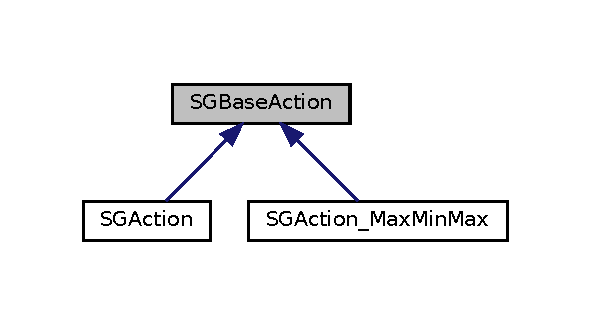
\includegraphics[width=284pt]{classSGBaseAction__inherit__graph}
\end{center}
\end{figure}


Collaboration diagram for S\+G\+Base\+Action\+:
\nopagebreak
\begin{figure}[H]
\begin{center}
\leavevmode
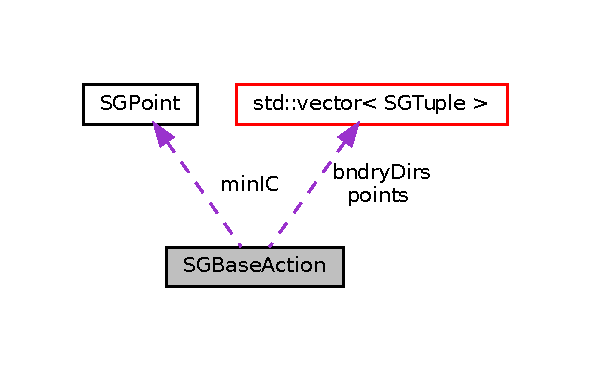
\includegraphics[width=284pt]{classSGBaseAction__coll__graph}
\end{center}
\end{figure}
\subsection*{Public Member Functions}
\begin{DoxyCompactItemize}
\item 
\hyperlink{classSGBaseAction_aa43b73172a811eb008f0762e405ae1a4}{S\+G\+Base\+Action} ()
\begin{DoxyCompactList}\small\item\em Constructor. \end{DoxyCompactList}\item 
\hyperlink{classSGBaseAction_a5f0a5c9866a41db2858d83a1f6aeed86}{S\+G\+Base\+Action} (int \+\_\+state, int \+\_\+action)
\begin{DoxyCompactList}\small\item\em Constructor. \end{DoxyCompactList}\item 
\hyperlink{classSGBaseAction_ad0e66183faa5ae137e075fe870f8cec9}{S\+G\+Base\+Action} (int \+\_\+num\+Players, int \+\_\+state, int \+\_\+action)
\begin{DoxyCompactList}\small\item\em Constructor. \end{DoxyCompactList}\item 
\mbox{\Hypertarget{classSGBaseAction_a66ef87852d14dc7970005ab2b801053e}\label{classSGBaseAction_a66ef87852d14dc7970005ab2b801053e}} 
\hyperlink{classSGBaseAction_a66ef87852d14dc7970005ab2b801053e}{$\sim$\+S\+G\+Base\+Action} ()
\begin{DoxyCompactList}\small\item\em Destructor. \end{DoxyCompactList}\item 
\mbox{\Hypertarget{classSGBaseAction_a99657086faa3d9d5d00b9c56c1b5e7bb}\label{classSGBaseAction_a99657086faa3d9d5d00b9c56c1b5e7bb}} 
bool \hyperlink{classSGBaseAction_a99657086faa3d9d5d00b9c56c1b5e7bb}{get\+Is\+Null} () const
\begin{DoxyCompactList}\small\item\em Returns true if the action is null. \end{DoxyCompactList}\item 
\mbox{\Hypertarget{classSGBaseAction_a91a8cce4f14293c47c7788d859284634}\label{classSGBaseAction_a91a8cce4f14293c47c7788d859284634}} 
int \hyperlink{classSGBaseAction_a91a8cce4f14293c47c7788d859284634}{get\+Action} () const
\begin{DoxyCompactList}\small\item\em Returns the action. \end{DoxyCompactList}\item 
\mbox{\Hypertarget{classSGBaseAction_a45df07dd310cdaf3bf15e18a894c9ac5}\label{classSGBaseAction_a45df07dd310cdaf3bf15e18a894c9ac5}} 
const vector$<$ \hyperlink{classSGTuple}{S\+G\+Tuple} $>$ \& \hyperlink{classSGBaseAction_a45df07dd310cdaf3bf15e18a894c9ac5}{get\+Points} () const
\begin{DoxyCompactList}\small\item\em Returns the points array. \end{DoxyCompactList}\item 
\mbox{\Hypertarget{classSGBaseAction_a7324f4465451d2ed6d3564c1090f35e7}\label{classSGBaseAction_a7324f4465451d2ed6d3564c1090f35e7}} 
const vector$<$ \hyperlink{classSGTuple}{S\+G\+Tuple} $>$ \& \hyperlink{classSGBaseAction_a7324f4465451d2ed6d3564c1090f35e7}{get\+Bndry\+Dirs} () const
\begin{DoxyCompactList}\small\item\em Get method for bndry dirs. \end{DoxyCompactList}\item 
\mbox{\Hypertarget{classSGBaseAction_a54af128dba67e36ba5dd41728ac4998b}\label{classSGBaseAction_a54af128dba67e36ba5dd41728ac4998b}} 
const vector$<$ vector$<$ int $>$ $>$ \& \hyperlink{classSGBaseAction_a54af128dba67e36ba5dd41728ac4998b}{get\+Tuples} () const
\begin{DoxyCompactList}\small\item\em Returns the tuples array. \end{DoxyCompactList}\item 
\mbox{\Hypertarget{classSGBaseAction_a8871a365591c09a8aae02eb2df29d7b8}\label{classSGBaseAction_a8871a365591c09a8aae02eb2df29d7b8}} 
int \hyperlink{classSGBaseAction_a8871a365591c09a8aae02eb2df29d7b8}{get\+State} () const
\begin{DoxyCompactList}\small\item\em Returns the state. \end{DoxyCompactList}\item 
\mbox{\Hypertarget{classSGBaseAction_ad23f122ff41f72b3cc161166905a13d8}\label{classSGBaseAction_ad23f122ff41f72b3cc161166905a13d8}} 
bool \hyperlink{classSGBaseAction_ad23f122ff41f72b3cc161166905a13d8}{has\+Corner} () const
\begin{DoxyCompactList}\small\item\em Returns whether or not the action has a corner. \end{DoxyCompactList}\item 
\mbox{\Hypertarget{classSGBaseAction_a860147b2ecb19aab60194ac0fe5f75db}\label{classSGBaseAction_a860147b2ecb19aab60194ac0fe5f75db}} 
const \hyperlink{classSGPoint}{S\+G\+Point} \& \hyperlink{classSGBaseAction_a860147b2ecb19aab60194ac0fe5f75db}{get\+Min\+I\+C\+Payoffs} () const
\begin{DoxyCompactList}\small\item\em Returns the minimum IC continuation values. \end{DoxyCompactList}\item 
\mbox{\Hypertarget{classSGBaseAction_a7b2874bed40408753e336084b13914aa}\label{classSGBaseAction_a7b2874bed40408753e336084b13914aa}} 
const vector$<$ \hyperlink{classSGTuple}{S\+G\+Tuple} $>$ \& \hyperlink{classSGBaseAction_a7b2874bed40408753e336084b13914aa}{get\+Binding\+Continuations} () const
\begin{DoxyCompactList}\small\item\em Returns the array of binding continuation values. \end{DoxyCompactList}\item 
\mbox{\Hypertarget{classSGBaseAction_aef9a88a93c5adcd164f0c30e3b006ae1}\label{classSGBaseAction_aef9a88a93c5adcd164f0c30e3b006ae1}} 
void \hyperlink{classSGBaseAction_aef9a88a93c5adcd164f0c30e3b006ae1}{set\+Min\+I\+C\+Payoffs} (const \hyperlink{classSGPoint}{S\+G\+Point} \&new\+Min\+IC)
\begin{DoxyCompactList}\small\item\em Sets the minimum IC continuation values. \end{DoxyCompactList}\item 
\mbox{\Hypertarget{classSGBaseAction_a06ba7b17e5c67aeeadb18c4767e319b3}\label{classSGBaseAction_a06ba7b17e5c67aeeadb18c4767e319b3}} 
void \hyperlink{classSGBaseAction_a06ba7b17e5c67aeeadb18c4767e319b3}{set\+Tuples} (const vector$<$ vector$<$ int $>$ $>$ \&new\+Tuples)
\begin{DoxyCompactList}\small\item\em Sets the tuples array. \end{DoxyCompactList}\item 
\mbox{\Hypertarget{classSGBaseAction_ae14aaa4093d68f14b8af1b3769ca084a}\label{classSGBaseAction_ae14aaa4093d68f14b8af1b3769ca084a}} 
void \hyperlink{classSGBaseAction_ae14aaa4093d68f14b8af1b3769ca084a}{set\+Points} (const vector$<$ \hyperlink{classSGTuple}{S\+G\+Tuple} $>$ \&new\+Points)
\begin{DoxyCompactList}\small\item\em Sets the points array. \end{DoxyCompactList}\item 
\mbox{\Hypertarget{classSGBaseAction_a991a8308a219ca7fadce3dcd5ae4ca71}\label{classSGBaseAction_a991a8308a219ca7fadce3dcd5ae4ca71}} 
void \hyperlink{classSGBaseAction_a991a8308a219ca7fadce3dcd5ae4ca71}{set\+Points\+And\+Tuples} (const vector$<$ \hyperlink{classSGTuple}{S\+G\+Tuple} $>$ \&new\+Points, const vector$<$ vector$<$ int $>$ $>$ \&new\+Tuples)
\begin{DoxyCompactList}\small\item\em Sets the points and tuples arrays. \end{DoxyCompactList}\item 
void \hyperlink{classSGBaseAction_a42092d69ccab82c32d31e2f762b669bd}{set\+Corner} (bool tf)
\begin{DoxyCompactList}\small\item\em Sets the corner indicator. \end{DoxyCompactList}\item 
\mbox{\Hypertarget{classSGBaseAction_ab46bc1f281b01c7289b2e7e68e64c4ac}\label{classSGBaseAction_ab46bc1f281b01c7289b2e7e68e64c4ac}} 
bool \hyperlink{classSGBaseAction_ab46bc1f281b01c7289b2e7e68e64c4ac}{is\+Corner} (const int p, const int k) const
\begin{DoxyCompactList}\small\item\em Returns whether or not the minimum IC payoff is feasible. \end{DoxyCompactList}\item 
\mbox{\Hypertarget{classSGBaseAction_a785478b3bafafb9cc502f92ec54a3b68}\label{classSGBaseAction_a785478b3bafafb9cc502f92ec54a3b68}} 
{\footnotesize template$<$class Archive $>$ }\\void \hyperlink{classSGBaseAction_a785478b3bafafb9cc502f92ec54a3b68}{serialize} (Archive \&ar, const unsigned int version)
\begin{DoxyCompactList}\small\item\em Serializes the action using the boost\+::serialization library. \end{DoxyCompactList}\end{DoxyCompactItemize}
\subsection*{Protected Attributes}
\begin{DoxyCompactItemize}
\item 
int \hyperlink{classSGBaseAction_a88066434fc68234175141e4bc19b1648}{num\+Players}
\item 
int \hyperlink{classSGBaseAction_a2301bf142f93f7d3ddedd44676d10c6a}{state}
\item 
int \hyperlink{classSGBaseAction_af293adc10da2dbb5a388a2fbcca0c67c}{action}
\item 
\hyperlink{classSGPoint}{S\+G\+Point} \hyperlink{classSGBaseAction_ae3bddc2bb5c5e108ead399e66f817b9b}{min\+IC}
\item 
vector$<$ \hyperlink{classSGTuple}{S\+G\+Tuple} $>$ \hyperlink{classSGBaseAction_a4d200e71f5bcfad3fe039293e90dbd70}{points}
\item 
vector$<$ \hyperlink{classSGTuple}{S\+G\+Tuple} $>$ \hyperlink{classSGBaseAction_a8854ab6cd8ad6d197b4647d60f093703}{bndry\+Dirs}
\item 
vector$<$ vector$<$ int $>$ $>$ \hyperlink{classSGBaseAction_a0cc43472c6c4cf598209d1e36eb28545}{tuples}
\item 
bool \hyperlink{classSGBaseAction_ad960a4cc7478182c36f9ebc534496150}{is\+Null}
\item 
bool \hyperlink{classSGBaseAction_a6b0251110d3c13dea965add5446bca40}{corner}
\end{DoxyCompactItemize}
\subsection*{Friends}
\begin{DoxyCompactItemize}
\item 
\mbox{\Hypertarget{classSGBaseAction_ac98d07dd8f7b70e16ccb9a01abf56b9c}\label{classSGBaseAction_ac98d07dd8f7b70e16ccb9a01abf56b9c}} 
class {\bfseries boost\+::serialization\+::access}
\end{DoxyCompactItemize}


\subsection{Detailed Description}
Describes an action in the game. 

Stores IC region information for a single action. Stores the action, minimum incentive compatible payoffs, points of intersection between the IC region and the expected feasible set, and indices of the tuples that generate the points of intersection. 

\subsection{Constructor \& Destructor Documentation}
\mbox{\Hypertarget{classSGBaseAction_aa43b73172a811eb008f0762e405ae1a4}\label{classSGBaseAction_aa43b73172a811eb008f0762e405ae1a4}} 
\index{S\+G\+Base\+Action@{S\+G\+Base\+Action}!S\+G\+Base\+Action@{S\+G\+Base\+Action}}
\index{S\+G\+Base\+Action@{S\+G\+Base\+Action}!S\+G\+Base\+Action@{S\+G\+Base\+Action}}
\subsubsection{\texorpdfstring{S\+G\+Base\+Action()}{SGBaseAction()}\hspace{0.1cm}{\footnotesize\ttfamily [1/3]}}
{\footnotesize\ttfamily S\+G\+Base\+Action\+::\+S\+G\+Base\+Action (\begin{DoxyParamCaption}{ }\end{DoxyParamCaption})\hspace{0.3cm}{\ttfamily [inline]}}



Constructor. 

Constructs a null action associated with the given \hyperlink{classSGEnv}{S\+G\+Env}. \mbox{\Hypertarget{classSGBaseAction_a5f0a5c9866a41db2858d83a1f6aeed86}\label{classSGBaseAction_a5f0a5c9866a41db2858d83a1f6aeed86}} 
\index{S\+G\+Base\+Action@{S\+G\+Base\+Action}!S\+G\+Base\+Action@{S\+G\+Base\+Action}}
\index{S\+G\+Base\+Action@{S\+G\+Base\+Action}!S\+G\+Base\+Action@{S\+G\+Base\+Action}}
\subsubsection{\texorpdfstring{S\+G\+Base\+Action()}{SGBaseAction()}\hspace{0.1cm}{\footnotesize\ttfamily [2/3]}}
{\footnotesize\ttfamily S\+G\+Base\+Action\+::\+S\+G\+Base\+Action (\begin{DoxyParamCaption}\item[{int}]{\+\_\+state,  }\item[{int}]{\+\_\+action }\end{DoxyParamCaption})\hspace{0.3cm}{\ttfamily [inline]}}



Constructor. 

Grandfather in two-\/player code. \mbox{\Hypertarget{classSGBaseAction_ad0e66183faa5ae137e075fe870f8cec9}\label{classSGBaseAction_ad0e66183faa5ae137e075fe870f8cec9}} 
\index{S\+G\+Base\+Action@{S\+G\+Base\+Action}!S\+G\+Base\+Action@{S\+G\+Base\+Action}}
\index{S\+G\+Base\+Action@{S\+G\+Base\+Action}!S\+G\+Base\+Action@{S\+G\+Base\+Action}}
\subsubsection{\texorpdfstring{S\+G\+Base\+Action()}{SGBaseAction()}\hspace{0.1cm}{\footnotesize\ttfamily [3/3]}}
{\footnotesize\ttfamily S\+G\+Base\+Action\+::\+S\+G\+Base\+Action (\begin{DoxyParamCaption}\item[{int}]{\+\_\+num\+Players,  }\item[{int}]{\+\_\+state,  }\item[{int}]{\+\_\+action }\end{DoxyParamCaption})\hspace{0.3cm}{\ttfamily [inline]}}



Constructor. 

Constructs an action for the given state and action index in the given environment. 

\subsection{Member Function Documentation}
\mbox{\Hypertarget{classSGBaseAction_a42092d69ccab82c32d31e2f762b669bd}\label{classSGBaseAction_a42092d69ccab82c32d31e2f762b669bd}} 
\index{S\+G\+Base\+Action@{S\+G\+Base\+Action}!set\+Corner@{set\+Corner}}
\index{set\+Corner@{set\+Corner}!S\+G\+Base\+Action@{S\+G\+Base\+Action}}
\subsubsection{\texorpdfstring{set\+Corner()}{setCorner()}}
{\footnotesize\ttfamily void S\+G\+Base\+Action\+::set\+Corner (\begin{DoxyParamCaption}\item[{bool}]{tf }\end{DoxyParamCaption})\hspace{0.3cm}{\ttfamily [inline]}}



Sets the corner indicator. 

$<$ Sets the indicator for whether there is a point at which both players constraints bind, when there are two players. 

\subsection{Member Data Documentation}
\mbox{\Hypertarget{classSGBaseAction_af293adc10da2dbb5a388a2fbcca0c67c}\label{classSGBaseAction_af293adc10da2dbb5a388a2fbcca0c67c}} 
\index{S\+G\+Base\+Action@{S\+G\+Base\+Action}!action@{action}}
\index{action@{action}!S\+G\+Base\+Action@{S\+G\+Base\+Action}}
\subsubsection{\texorpdfstring{action}{action}}
{\footnotesize\ttfamily int S\+G\+Base\+Action\+::action\hspace{0.3cm}{\ttfamily [protected]}}

The index of the action profile. \mbox{\Hypertarget{classSGBaseAction_a8854ab6cd8ad6d197b4647d60f093703}\label{classSGBaseAction_a8854ab6cd8ad6d197b4647d60f093703}} 
\index{S\+G\+Base\+Action@{S\+G\+Base\+Action}!bndry\+Dirs@{bndry\+Dirs}}
\index{bndry\+Dirs@{bndry\+Dirs}!S\+G\+Base\+Action@{S\+G\+Base\+Action}}
\subsubsection{\texorpdfstring{bndry\+Dirs}{bndryDirs}}
{\footnotesize\ttfamily vector$<$\hyperlink{classSGTuple}{S\+G\+Tuple}$>$ S\+G\+Base\+Action\+::bndry\+Dirs\hspace{0.3cm}{\ttfamily [protected]}}

Stores the slope of the frontier at the extreme payoffs. \mbox{\Hypertarget{classSGBaseAction_a6b0251110d3c13dea965add5446bca40}\label{classSGBaseAction_a6b0251110d3c13dea965add5446bca40}} 
\index{S\+G\+Base\+Action@{S\+G\+Base\+Action}!corner@{corner}}
\index{corner@{corner}!S\+G\+Base\+Action@{S\+G\+Base\+Action}}
\subsubsection{\texorpdfstring{corner}{corner}}
{\footnotesize\ttfamily bool S\+G\+Base\+Action\+::corner\hspace{0.3cm}{\ttfamily [protected]}}

Flag that indicates that the minimum IC continuation value is feasible. \mbox{\Hypertarget{classSGBaseAction_ad960a4cc7478182c36f9ebc534496150}\label{classSGBaseAction_ad960a4cc7478182c36f9ebc534496150}} 
\index{S\+G\+Base\+Action@{S\+G\+Base\+Action}!is\+Null@{is\+Null}}
\index{is\+Null@{is\+Null}!S\+G\+Base\+Action@{S\+G\+Base\+Action}}
\subsubsection{\texorpdfstring{is\+Null}{isNull}}
{\footnotesize\ttfamily bool S\+G\+Base\+Action\+::is\+Null\hspace{0.3cm}{\ttfamily [protected]}}

Flag to indicate that this is the place holder \char`\"{}null\char`\"{} action. \mbox{\Hypertarget{classSGBaseAction_ae3bddc2bb5c5e108ead399e66f817b9b}\label{classSGBaseAction_ae3bddc2bb5c5e108ead399e66f817b9b}} 
\index{S\+G\+Base\+Action@{S\+G\+Base\+Action}!min\+IC@{min\+IC}}
\index{min\+IC@{min\+IC}!S\+G\+Base\+Action@{S\+G\+Base\+Action}}
\subsubsection{\texorpdfstring{min\+IC}{minIC}}
{\footnotesize\ttfamily \hyperlink{classSGPoint}{S\+G\+Point} S\+G\+Base\+Action\+::min\+IC\hspace{0.3cm}{\ttfamily [protected]}}

The minimum continuation value to support incentive compatibility, relative to the current threat tuple. In particular, this is the maximum over all deviations of the expected threat point under the deviation, plus (1-\/delta)/delta times the static gains from deviating. \mbox{\Hypertarget{classSGBaseAction_a88066434fc68234175141e4bc19b1648}\label{classSGBaseAction_a88066434fc68234175141e4bc19b1648}} 
\index{S\+G\+Base\+Action@{S\+G\+Base\+Action}!num\+Players@{num\+Players}}
\index{num\+Players@{num\+Players}!S\+G\+Base\+Action@{S\+G\+Base\+Action}}
\subsubsection{\texorpdfstring{num\+Players}{numPlayers}}
{\footnotesize\ttfamily int S\+G\+Base\+Action\+::num\+Players\hspace{0.3cm}{\ttfamily [protected]}}

Should be two or three in all current implementations. \mbox{\Hypertarget{classSGBaseAction_a4d200e71f5bcfad3fe039293e90dbd70}\label{classSGBaseAction_a4d200e71f5bcfad3fe039293e90dbd70}} 
\index{S\+G\+Base\+Action@{S\+G\+Base\+Action}!points@{points}}
\index{points@{points}!S\+G\+Base\+Action@{S\+G\+Base\+Action}}
\subsubsection{\texorpdfstring{points}{points}}
{\footnotesize\ttfamily vector$<$ \hyperlink{classSGTuple}{S\+G\+Tuple} $>$ S\+G\+Base\+Action\+::points\hspace{0.3cm}{\ttfamily [protected]}}

Extreme points of the set of expected feasible continuation values at which some player\textquotesingle{}s incentive constraint binds. points\mbox{[}i\mbox{]} is an \hyperlink{classSGTuple}{S\+G\+Tuple} consisting of either 0 or 2 \hyperlink{classSGPoint}{S\+G\+Point} objects, which are the extreme binding payoffs on player i\textquotesingle{}s incentive constraint. The convention is that the first element of the tuple is the northern or easternmost of the two binding payoffs. \mbox{\Hypertarget{classSGBaseAction_a2301bf142f93f7d3ddedd44676d10c6a}\label{classSGBaseAction_a2301bf142f93f7d3ddedd44676d10c6a}} 
\index{S\+G\+Base\+Action@{S\+G\+Base\+Action}!state@{state}}
\index{state@{state}!S\+G\+Base\+Action@{S\+G\+Base\+Action}}
\subsubsection{\texorpdfstring{state}{state}}
{\footnotesize\ttfamily int S\+G\+Base\+Action\+::state\hspace{0.3cm}{\ttfamily [protected]}}

The state in which this action profile can be played. \mbox{\Hypertarget{classSGBaseAction_a0cc43472c6c4cf598209d1e36eb28545}\label{classSGBaseAction_a0cc43472c6c4cf598209d1e36eb28545}} 
\index{S\+G\+Base\+Action@{S\+G\+Base\+Action}!tuples@{tuples}}
\index{tuples@{tuples}!S\+G\+Base\+Action@{S\+G\+Base\+Action}}
\subsubsection{\texorpdfstring{tuples}{tuples}}
{\footnotesize\ttfamily vector$<$ vector$<$ int $>$ $>$ S\+G\+Base\+Action\+::tuples\hspace{0.3cm}{\ttfamily [protected]}}

The vector tuples\mbox{[}i\mbox{]}\mbox{[}j\mbox{]} points to the element of S\+G\+Approximation\+::extreme\+Tuples whose expectation is just clockwise relative to points\mbox{[}i\mbox{]}\mbox{[}j\mbox{]}. 

The documentation for this class was generated from the following files\+:\begin{DoxyCompactItemize}
\item 
src/hpp/sgbaseaction.\+hpp\item 
src/cpp/sgbaseaction.\+cpp\end{DoxyCompactItemize}

\hypertarget{classSGBoolParamBox}{}\section{S\+G\+Bool\+Param\+Box Class Reference}
\label{classSGBoolParamBox}\index{S\+G\+Bool\+Param\+Box@{S\+G\+Bool\+Param\+Box}}


Class for changing boolean parameters.  




{\ttfamily \#include $<$sgsettingshandler.\+hpp$>$}



Inheritance diagram for S\+G\+Bool\+Param\+Box\+:
\nopagebreak
\begin{figure}[H]
\begin{center}
\leavevmode
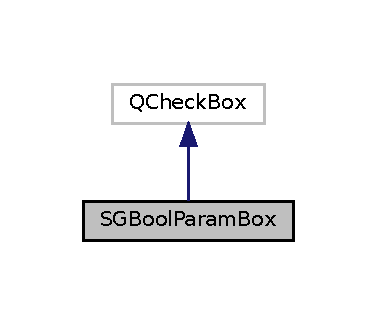
\includegraphics[width=181pt]{classSGBoolParamBox__inherit__graph}
\end{center}
\end{figure}


Collaboration diagram for S\+G\+Bool\+Param\+Box\+:
\nopagebreak
\begin{figure}[H]
\begin{center}
\leavevmode
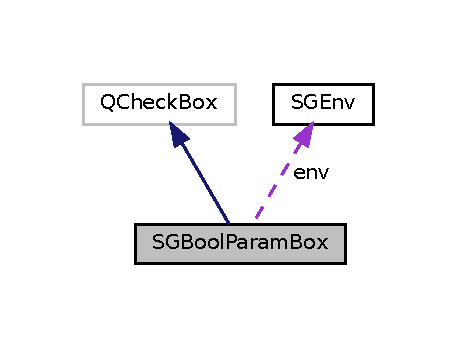
\includegraphics[width=220pt]{classSGBoolParamBox__coll__graph}
\end{center}
\end{figure}
\subsection*{Public Member Functions}
\begin{DoxyCompactItemize}
\item 
\mbox{\Hypertarget{classSGBoolParamBox_a7dbba884d15e63ac6302672a0526d689}\label{classSGBoolParamBox_a7dbba884d15e63ac6302672a0526d689}} 
\hyperlink{classSGBoolParamBox_a7dbba884d15e63ac6302672a0526d689}{S\+G\+Bool\+Param\+Box} (Q\+Widget $\ast$parent, \hyperlink{classSGEnv}{S\+G\+Env} $\ast$\+\_\+env, \hyperlink{namespaceSG_a0b164afe6c58be3386d9e3f6e857b673}{S\+G\+::\+B\+O\+O\+L\+\_\+\+P\+A\+R\+AM} \+\_\+param)
\begin{DoxyCompactList}\small\item\em Constructor. \end{DoxyCompactList}\end{DoxyCompactItemize}
\subsection*{Private Slots}
\begin{DoxyCompactItemize}
\item 
\mbox{\Hypertarget{classSGBoolParamBox_a1cb3236565d114c247b82ee9b5a344e7}\label{classSGBoolParamBox_a1cb3236565d114c247b82ee9b5a344e7}} 
void \hyperlink{classSGBoolParamBox_a1cb3236565d114c247b82ee9b5a344e7}{change\+Param} ()
\begin{DoxyCompactList}\small\item\em Slot called when the check is modified. \end{DoxyCompactList}\item 
\mbox{\Hypertarget{classSGBoolParamBox_a80b6c9d3e08126850ce592e395cbe6f7}\label{classSGBoolParamBox_a80b6c9d3e08126850ce592e395cbe6f7}} 
void \hyperlink{classSGBoolParamBox_a80b6c9d3e08126850ce592e395cbe6f7}{reset\+Param} ()
\begin{DoxyCompactList}\small\item\em Slot called when resetting to default values. \end{DoxyCompactList}\end{DoxyCompactItemize}
\subsection*{Private Member Functions}
\begin{DoxyCompactItemize}
\item 
\mbox{\Hypertarget{classSGBoolParamBox_a325cf165100d961ef33c77001b42270e}\label{classSGBoolParamBox_a325cf165100d961ef33c77001b42270e}} 
void \hyperlink{classSGBoolParamBox_a325cf165100d961ef33c77001b42270e}{set\+Check} (bool tf)
\begin{DoxyCompactList}\small\item\em The set method. \end{DoxyCompactList}\end{DoxyCompactItemize}
\subsection*{Private Attributes}
\begin{DoxyCompactItemize}
\item 
\mbox{\Hypertarget{classSGBoolParamBox_a490e196a9b5942edf920d16a83ff9a98}\label{classSGBoolParamBox_a490e196a9b5942edf920d16a83ff9a98}} 
\hyperlink{namespaceSG_a0b164afe6c58be3386d9e3f6e857b673}{S\+G\+::\+B\+O\+O\+L\+\_\+\+P\+A\+R\+AM} \hyperlink{classSGBoolParamBox_a490e196a9b5942edf920d16a83ff9a98}{param}
\begin{DoxyCompactList}\small\item\em The boolean parameter associated with the box. \end{DoxyCompactList}\item 
\mbox{\Hypertarget{classSGBoolParamBox_aa3592842bf61b151242c99cf8bc3517a}\label{classSGBoolParamBox_aa3592842bf61b151242c99cf8bc3517a}} 
\hyperlink{classSGEnv}{S\+G\+Env} $\ast$ \hyperlink{classSGBoolParamBox_aa3592842bf61b151242c99cf8bc3517a}{env}
\begin{DoxyCompactList}\small\item\em The associated environment. \end{DoxyCompactList}\end{DoxyCompactItemize}


\subsection{Detailed Description}
Class for changing boolean parameters. 

A customized version of Q\+Check\+Box for modifying boolean parameters in an \hyperlink{classSGEnv}{S\+G\+Env} object that is used by the \hyperlink{classSGSettingsHandler}{S\+G\+Settings\+Handler}. It has a private members which are the particular \hyperlink{namespaceSG_a0b164afe6c58be3386d9e3f6e857b673}{S\+G\+::\+B\+O\+O\+L\+\_\+\+P\+A\+R\+AM} that is associated with this edit and a pointer to an associated \hyperlink{classSGEnv}{S\+G\+Env} object. There are also mutator methods for setting the parameter value and resetting to the default value of the given parameter. 

The documentation for this class was generated from the following file\+:\begin{DoxyCompactItemize}
\item 
viewer/hpp/sgsettingshandler.\+hpp\end{DoxyCompactItemize}

\hypertarget{classSGCustomPlot}{}\section{S\+G\+Custom\+Plot Class Reference}
\label{classSGCustomPlot}\index{S\+G\+Custom\+Plot@{S\+G\+Custom\+Plot}}


A customized version of Q\+Custom\+Plot.  




{\ttfamily \#include $<$sgcustomplot.\+hpp$>$}



Inheritance diagram for S\+G\+Custom\+Plot\+:
\nopagebreak
\begin{figure}[H]
\begin{center}
\leavevmode
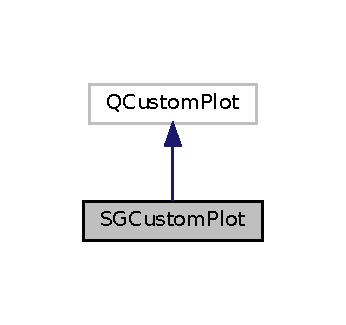
\includegraphics[width=166pt]{classSGCustomPlot__inherit__graph}
\end{center}
\end{figure}


Collaboration diagram for S\+G\+Custom\+Plot\+:
\nopagebreak
\begin{figure}[H]
\begin{center}
\leavevmode
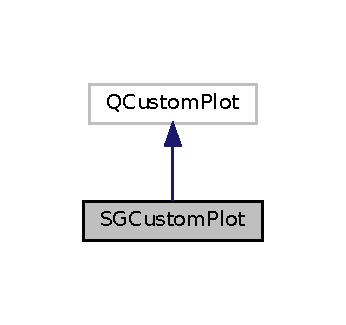
\includegraphics[width=166pt]{classSGCustomPlot__coll__graph}
\end{center}
\end{figure}
\subsection*{Signals}
\begin{DoxyCompactItemize}
\item 
\mbox{\Hypertarget{classSGCustomPlot_a23f808cae1e818047ef19fb2f81b2640}\label{classSGCustomPlot_a23f808cae1e818047ef19fb2f81b2640}} 
void \hyperlink{classSGCustomPlot_a23f808cae1e818047ef19fb2f81b2640}{inspect\+Point} (\hyperlink{classSGPoint}{S\+G\+Point} point, int \hyperlink{classSGCustomPlot_ac17b8dfc3d9579e6286efa060ca55ab0}{state}, bool \hyperlink{classSGCustomPlot_a216325e80035b2042215a6ad9cd82202}{is\+Detail\+Plot})
\begin{DoxyCompactList}\small\item\em Signal to inspect the given point. \end{DoxyCompactList}\item 
\mbox{\Hypertarget{classSGCustomPlot_ab8369e075314ff6d557f433b25b6852c}\label{classSGCustomPlot_ab8369e075314ff6d557f433b25b6852c}} 
void \hyperlink{classSGCustomPlot_ab8369e075314ff6d557f433b25b6852c}{simulate\+Equilibrium} (\hyperlink{classSGPoint}{S\+G\+Point} point, int \hyperlink{classSGCustomPlot_ac17b8dfc3d9579e6286efa060ca55ab0}{state}, bool \hyperlink{classSGCustomPlot_a216325e80035b2042215a6ad9cd82202}{is\+Detail\+Plot})
\begin{DoxyCompactList}\small\item\em Signal to simulate the given equilibrium forwards. \end{DoxyCompactList}\end{DoxyCompactItemize}
\subsection*{Public Member Functions}
\begin{DoxyCompactItemize}
\item 
\mbox{\Hypertarget{classSGCustomPlot_a5a4641a2110a34cb967b5de276f5f457}\label{classSGCustomPlot_a5a4641a2110a34cb967b5de276f5f457}} 
\hyperlink{classSGCustomPlot_a5a4641a2110a34cb967b5de276f5f457}{S\+G\+Custom\+Plot} ()
\begin{DoxyCompactList}\small\item\em Constructor. \end{DoxyCompactList}\item 
\hyperlink{classSGCustomPlot_a95ebb2e31d5aa9bcbd850bb99c5e6d95}{S\+G\+Custom\+Plot} (int \+\_\+state, bool \+\_\+is\+Detail\+Plot)
\begin{DoxyCompactList}\small\item\em Constructor. \end{DoxyCompactList}\item 
\mbox{\Hypertarget{classSGCustomPlot_a9ef7a8ce9d52fab259120958b3596622}\label{classSGCustomPlot_a9ef7a8ce9d52fab259120958b3596622}} 
Q\+C\+P\+Plot\+Title $\ast$ \hyperlink{classSGCustomPlot_a9ef7a8ce9d52fab259120958b3596622}{get\+Title} ()
\begin{DoxyCompactList}\small\item\em Returns the title. \end{DoxyCompactList}\item 
\mbox{\Hypertarget{classSGCustomPlot_a318a8971c236a0f675bdc28bebdecc12}\label{classSGCustomPlot_a318a8971c236a0f675bdc28bebdecc12}} 
void \hyperlink{classSGCustomPlot_a318a8971c236a0f675bdc28bebdecc12}{adjust\+Ranges} ()
\begin{DoxyCompactList}\small\item\em Updates ranges when window is resized. \end{DoxyCompactList}\item 
void \hyperlink{classSGCustomPlot_ad20fcf8ce5db4628acdddae73238301c}{set\+Ranges} (const Q\+C\+P\+Range \&xrange, const Q\+C\+P\+Range \&yrange)
\begin{DoxyCompactList}\small\item\em Sets the nominal ranges. \end{DoxyCompactList}\item 
\mbox{\Hypertarget{classSGCustomPlot_abc4224d3185bed305f40646626e30625}\label{classSGCustomPlot_abc4224d3185bed305f40646626e30625}} 
const Q\+C\+P\+Range \& \hyperlink{classSGCustomPlot_abc4224d3185bed305f40646626e30625}{get\+Nominal\+X\+Range} () const
\begin{DoxyCompactList}\small\item\em Returns the nominal X range. \end{DoxyCompactList}\item 
\mbox{\Hypertarget{classSGCustomPlot_a52e0a60a726ebd157839b013af068420}\label{classSGCustomPlot_a52e0a60a726ebd157839b013af068420}} 
const Q\+C\+P\+Range \& \hyperlink{classSGCustomPlot_a52e0a60a726ebd157839b013af068420}{get\+Nominal\+Y\+Range} () const
\begin{DoxyCompactList}\small\item\em Returns the nominal Y range. \end{DoxyCompactList}\item 
\mbox{\Hypertarget{classSGCustomPlot_ae69a5b83aab673e813bc48c9e5b8a0bd}\label{classSGCustomPlot_ae69a5b83aab673e813bc48c9e5b8a0bd}} 
void \hyperlink{classSGCustomPlot_ae69a5b83aab673e813bc48c9e5b8a0bd}{equalize\+Axes\+Scales} ()
\begin{DoxyCompactList}\small\item\em Normalize ranges. \end{DoxyCompactList}\item 
\mbox{\Hypertarget{classSGCustomPlot_a7583d7141ffd1a751f01f22b23c50e5a}\label{classSGCustomPlot_a7583d7141ffd1a751f01f22b23c50e5a}} 
void \hyperlink{classSGCustomPlot_a7583d7141ffd1a751f01f22b23c50e5a}{set\+State} (int new\+State)
\begin{DoxyCompactList}\small\item\em Sets the state associated with the plot. \end{DoxyCompactList}\item 
\mbox{\Hypertarget{classSGCustomPlot_a5a23324945745f0af195e25b70814637}\label{classSGCustomPlot_a5a23324945745f0af195e25b70814637}} 
int \hyperlink{classSGCustomPlot_a5a23324945745f0af195e25b70814637}{get\+State} () const
\begin{DoxyCompactList}\small\item\em Gets the state associated with the plot. \end{DoxyCompactList}\end{DoxyCompactItemize}
\subsection*{Protected Member Functions}
\begin{DoxyCompactItemize}
\item 
void \hyperlink{classSGCustomPlot_a4f1dee38be23b4b3fbe46cab9c6db6d7}{resize\+Event} (Q\+Resize\+Event $\ast$event)
\begin{DoxyCompactList}\small\item\em Reimplement resize\+Event. \end{DoxyCompactList}\end{DoxyCompactItemize}
\subsection*{Private Slots}
\begin{DoxyCompactItemize}
\item 
void \hyperlink{classSGCustomPlot_a9e8312d8b4cc19d53bc8790b71f3e8ed}{Show\+Context\+Menu} (const Q\+Point \&pos)
\begin{DoxyCompactList}\small\item\em Slot for showing context menu. \end{DoxyCompactList}\item 
\mbox{\Hypertarget{classSGCustomPlot_ab63f0da26acab2aa7295d44c9a3d5203}\label{classSGCustomPlot_ab63f0da26acab2aa7295d44c9a3d5203}} 
void \hyperlink{classSGCustomPlot_ab63f0da26acab2aa7295d44c9a3d5203}{point\+Inspected} ()
\begin{DoxyCompactList}\small\item\em Point inspected. \end{DoxyCompactList}\item 
\mbox{\Hypertarget{classSGCustomPlot_a6068b1ffa202245fa8eeb594e6860bb9}\label{classSGCustomPlot_a6068b1ffa202245fa8eeb594e6860bb9}} 
void {\bfseries simulation\+Requested} ()
\item 
\mbox{\Hypertarget{classSGCustomPlot_a9108592865d386c9fafaeac1b813848c}\label{classSGCustomPlot_a9108592865d386c9fafaeac1b813848c}} 
void \hyperlink{classSGCustomPlot_a9108592865d386c9fafaeac1b813848c}{save\+P\+DF} ()
\begin{DoxyCompactList}\small\item\em Saves graph as a P\+DF. \end{DoxyCompactList}\item 
\mbox{\Hypertarget{classSGCustomPlot_a18f01b1582f9b0415f4b32841846c8dc}\label{classSGCustomPlot_a18f01b1582f9b0415f4b32841846c8dc}} 
void \hyperlink{classSGCustomPlot_a18f01b1582f9b0415f4b32841846c8dc}{save\+P\+NG} ()
\begin{DoxyCompactList}\small\item\em Saves graph as a P\+NG. \end{DoxyCompactList}\end{DoxyCompactItemize}
\subsection*{Private Member Functions}
\begin{DoxyCompactItemize}
\item 
virtual int \hyperlink{classSGCustomPlot_ad60d048905082b37f4a15bd1644f8717}{height\+For\+Width} (int w) const
\begin{DoxyCompactList}\small\item\em Reimplement height\+For\+Width. \end{DoxyCompactList}\item 
virtual bool \hyperlink{classSGCustomPlot_a560baf18b0aa2e31631c603abfa74d47}{has\+Height\+For\+Width} () const
\begin{DoxyCompactList}\small\item\em Reimplement has\+Heigh\+For\+Width. \end{DoxyCompactList}\item 
\mbox{\Hypertarget{classSGCustomPlot_a2779f4bb4a1b5504c9e4f58bd545df24}\label{classSGCustomPlot_a2779f4bb4a1b5504c9e4f58bd545df24}} 
virtual Q\+Size \hyperlink{classSGCustomPlot_a2779f4bb4a1b5504c9e4f58bd545df24}{minimum\+Size\+Hint} () const
\begin{DoxyCompactList}\small\item\em Custom minimum size. \end{DoxyCompactList}\end{DoxyCompactItemize}
\subsection*{Private Attributes}
\begin{DoxyCompactItemize}
\item 
\mbox{\Hypertarget{classSGCustomPlot_ac17b8dfc3d9579e6286efa060ca55ab0}\label{classSGCustomPlot_ac17b8dfc3d9579e6286efa060ca55ab0}} 
int \hyperlink{classSGCustomPlot_ac17b8dfc3d9579e6286efa060ca55ab0}{state}
\begin{DoxyCompactList}\small\item\em Indicates the state that this plot is associated with. \end{DoxyCompactList}\item 
\mbox{\Hypertarget{classSGCustomPlot_a216325e80035b2042215a6ad9cd82202}\label{classSGCustomPlot_a216325e80035b2042215a6ad9cd82202}} 
bool \hyperlink{classSGCustomPlot_a216325e80035b2042215a6ad9cd82202}{is\+Detail\+Plot}
\begin{DoxyCompactList}\small\item\em Indicates if this is the detail plot. \end{DoxyCompactList}\item 
Q\+C\+P\+Plot\+Title $\ast$ \hyperlink{classSGCustomPlot_a230237a7692e75bfe15e250342bfd801}{title}
\item 
Q\+C\+P\+Range \hyperlink{classSGCustomPlot_a255402d40b328430c649c878ee593b11}{nominal\+X\+Range}
\item 
Q\+C\+P\+Range \hyperlink{classSGCustomPlot_a4d7a4961ec0e095a9c3582060bc9cbd2}{nominal\+Y\+Range}
\item 
Q\+C\+P\+Range \hyperlink{classSGCustomPlot_a96f63b86fe49372586cb6be908d88bc4}{real\+X\+Range}
\item 
Q\+C\+P\+Range \hyperlink{classSGCustomPlot_aeffca93d0d63a439e3c3bf35d18fa698}{real\+Y\+Range}
\item 
Q\+String \hyperlink{classSGCustomPlot_a9051f043c91f3e59fbc1c2a818c76687}{path}
\begin{DoxyCompactList}\small\item\em Save file path. \end{DoxyCompactList}\item 
\mbox{\Hypertarget{classSGCustomPlot_a73fd511ad74d3db5433f51f8a75a5f92}\label{classSGCustomPlot_a73fd511ad74d3db5433f51f8a75a5f92}} 
Q\+Action $\ast$ \hyperlink{classSGCustomPlot_a73fd511ad74d3db5433f51f8a75a5f92}{inspect\+Point\+Action}
\begin{DoxyCompactList}\small\item\em Inspect a point. \end{DoxyCompactList}\item 
\mbox{\Hypertarget{classSGCustomPlot_aa33a8ed74cad0d2e0ef1b1d4e2af6a31}\label{classSGCustomPlot_aa33a8ed74cad0d2e0ef1b1d4e2af6a31}} 
Q\+Action $\ast$ \hyperlink{classSGCustomPlot_aa33a8ed74cad0d2e0ef1b1d4e2af6a31}{simulate\+Action}
\begin{DoxyCompactList}\small\item\em Action for forward simulating. \end{DoxyCompactList}\item 
\mbox{\Hypertarget{classSGCustomPlot_ac20df7cd696ea2b61c78606589f5e726}\label{classSGCustomPlot_ac20df7cd696ea2b61c78606589f5e726}} 
Q\+Action $\ast$ \hyperlink{classSGCustomPlot_ac20df7cd696ea2b61c78606589f5e726}{save\+P\+N\+G\+Action}
\begin{DoxyCompactList}\small\item\em Pointer to the Q\+Action for saving P\+NG files. \end{DoxyCompactList}\item 
\mbox{\Hypertarget{classSGCustomPlot_a9df5c584b4b967e80d3a56b0e2f7fef1}\label{classSGCustomPlot_a9df5c584b4b967e80d3a56b0e2f7fef1}} 
Q\+Action $\ast$ \hyperlink{classSGCustomPlot_a9df5c584b4b967e80d3a56b0e2f7fef1}{save\+P\+D\+F\+Action}
\begin{DoxyCompactList}\small\item\em Pointer to the Q\+Action for saving P\+DF files. \end{DoxyCompactList}\item 
\mbox{\Hypertarget{classSGCustomPlot_ac3903a96504ec5d4e4a5c76e1fe602c7}\label{classSGCustomPlot_ac3903a96504ec5d4e4a5c76e1fe602c7}} 
Q\+Point \hyperlink{classSGCustomPlot_ac3903a96504ec5d4e4a5c76e1fe602c7}{last\+Context\+Pos}
\begin{DoxyCompactList}\small\item\em Stores the last location at which a context menu was requested. \end{DoxyCompactList}\end{DoxyCompactItemize}


\subsection{Detailed Description}
A customized version of Q\+Custom\+Plot. 

This class inherits from Q\+Custom\+Plot and adds functionality for controling ranges to maintain the desired aspect ratio. It also adds functionality for right-\/clicking on the plot to bring up a context menu. This menu has various options, some of which pertain to the payoffs closest to where the user clicked. In particular, there are signals for saving copys of the plots, for \char`\"{}inspecting\char`\"{} a given payoff vector, and for initializing the \hyperlink{classSGSimulationHandler}{S\+G\+Simulation\+Handler} to forward simulate the equilibrium that generates the given payoffs. 

\subsection{Constructor \& Destructor Documentation}
\mbox{\Hypertarget{classSGCustomPlot_a95ebb2e31d5aa9bcbd850bb99c5e6d95}\label{classSGCustomPlot_a95ebb2e31d5aa9bcbd850bb99c5e6d95}} 
\index{S\+G\+Custom\+Plot@{S\+G\+Custom\+Plot}!S\+G\+Custom\+Plot@{S\+G\+Custom\+Plot}}
\index{S\+G\+Custom\+Plot@{S\+G\+Custom\+Plot}!S\+G\+Custom\+Plot@{S\+G\+Custom\+Plot}}
\subsubsection{\texorpdfstring{S\+G\+Custom\+Plot()}{SGCustomPlot()}}
{\footnotesize\ttfamily S\+G\+Custom\+Plot\+::\+S\+G\+Custom\+Plot (\begin{DoxyParamCaption}\item[{int}]{\+\_\+state,  }\item[{bool}]{\+\_\+is\+Detail\+Plot }\end{DoxyParamCaption})}



Constructor. 

Sets the state and whether or not is the detail\+Plot. Also initializes the plot and connect slots to actions. 

\subsection{Member Function Documentation}
\mbox{\Hypertarget{classSGCustomPlot_a560baf18b0aa2e31631c603abfa74d47}\label{classSGCustomPlot_a560baf18b0aa2e31631c603abfa74d47}} 
\index{S\+G\+Custom\+Plot@{S\+G\+Custom\+Plot}!has\+Height\+For\+Width@{has\+Height\+For\+Width}}
\index{has\+Height\+For\+Width@{has\+Height\+For\+Width}!S\+G\+Custom\+Plot@{S\+G\+Custom\+Plot}}
\subsubsection{\texorpdfstring{has\+Height\+For\+Width()}{hasHeightForWidth()}}
{\footnotesize\ttfamily virtual bool S\+G\+Custom\+Plot\+::has\+Height\+For\+Width (\begin{DoxyParamCaption}{ }\end{DoxyParamCaption}) const\hspace{0.3cm}{\ttfamily [inline]}, {\ttfamily [private]}, {\ttfamily [virtual]}}



Reimplement has\+Heigh\+For\+Width. 

Indicates that height\+For\+Width has been reimplemented. \mbox{\Hypertarget{classSGCustomPlot_ad60d048905082b37f4a15bd1644f8717}\label{classSGCustomPlot_ad60d048905082b37f4a15bd1644f8717}} 
\index{S\+G\+Custom\+Plot@{S\+G\+Custom\+Plot}!height\+For\+Width@{height\+For\+Width}}
\index{height\+For\+Width@{height\+For\+Width}!S\+G\+Custom\+Plot@{S\+G\+Custom\+Plot}}
\subsubsection{\texorpdfstring{height\+For\+Width()}{heightForWidth()}}
{\footnotesize\ttfamily virtual int S\+G\+Custom\+Plot\+::height\+For\+Width (\begin{DoxyParamCaption}\item[{int}]{w }\end{DoxyParamCaption}) const\hspace{0.3cm}{\ttfamily [inline]}, {\ttfamily [private]}, {\ttfamily [virtual]}}



Reimplement height\+For\+Width. 

Suggests a square aspect ratio. \mbox{\Hypertarget{classSGCustomPlot_a4f1dee38be23b4b3fbe46cab9c6db6d7}\label{classSGCustomPlot_a4f1dee38be23b4b3fbe46cab9c6db6d7}} 
\index{S\+G\+Custom\+Plot@{S\+G\+Custom\+Plot}!resize\+Event@{resize\+Event}}
\index{resize\+Event@{resize\+Event}!S\+G\+Custom\+Plot@{S\+G\+Custom\+Plot}}
\subsubsection{\texorpdfstring{resize\+Event()}{resizeEvent()}}
{\footnotesize\ttfamily void S\+G\+Custom\+Plot\+::resize\+Event (\begin{DoxyParamCaption}\item[{Q\+Resize\+Event $\ast$}]{event }\end{DoxyParamCaption})\hspace{0.3cm}{\ttfamily [inline]}, {\ttfamily [protected]}}



Reimplement resize\+Event. 

Calls adjust ranges before calling Q\+Custom\+Plot\+::resize\+Event. \mbox{\Hypertarget{classSGCustomPlot_ad20fcf8ce5db4628acdddae73238301c}\label{classSGCustomPlot_ad20fcf8ce5db4628acdddae73238301c}} 
\index{S\+G\+Custom\+Plot@{S\+G\+Custom\+Plot}!set\+Ranges@{set\+Ranges}}
\index{set\+Ranges@{set\+Ranges}!S\+G\+Custom\+Plot@{S\+G\+Custom\+Plot}}
\subsubsection{\texorpdfstring{set\+Ranges()}{setRanges()}}
{\footnotesize\ttfamily void S\+G\+Custom\+Plot\+::set\+Ranges (\begin{DoxyParamCaption}\item[{const Q\+C\+P\+Range \&}]{xrange,  }\item[{const Q\+C\+P\+Range \&}]{yrange }\end{DoxyParamCaption})}



Sets the nominal ranges. 

Constructor. \mbox{\Hypertarget{classSGCustomPlot_a9e8312d8b4cc19d53bc8790b71f3e8ed}\label{classSGCustomPlot_a9e8312d8b4cc19d53bc8790b71f3e8ed}} 
\index{S\+G\+Custom\+Plot@{S\+G\+Custom\+Plot}!Show\+Context\+Menu@{Show\+Context\+Menu}}
\index{Show\+Context\+Menu@{Show\+Context\+Menu}!S\+G\+Custom\+Plot@{S\+G\+Custom\+Plot}}
\subsubsection{\texorpdfstring{Show\+Context\+Menu}{ShowContextMenu}}
{\footnotesize\ttfamily void S\+G\+Custom\+Plot\+::\+Show\+Context\+Menu (\begin{DoxyParamCaption}\item[{const Q\+Point \&}]{pos }\end{DoxyParamCaption})\hspace{0.3cm}{\ttfamily [inline]}, {\ttfamily [private]}, {\ttfamily [slot]}}



Slot for showing context menu. 

Creates a context menu and shows the actions for saving P\+D\+F/\+P\+NG files. 

\subsection{Member Data Documentation}
\mbox{\Hypertarget{classSGCustomPlot_a255402d40b328430c649c878ee593b11}\label{classSGCustomPlot_a255402d40b328430c649c878ee593b11}} 
\index{S\+G\+Custom\+Plot@{S\+G\+Custom\+Plot}!nominal\+X\+Range@{nominal\+X\+Range}}
\index{nominal\+X\+Range@{nominal\+X\+Range}!S\+G\+Custom\+Plot@{S\+G\+Custom\+Plot}}
\subsubsection{\texorpdfstring{nominal\+X\+Range}{nominalXRange}}
{\footnotesize\ttfamily Q\+C\+P\+Range S\+G\+Custom\+Plot\+::nominal\+X\+Range\hspace{0.3cm}{\ttfamily [private]}}

Nominal X range. \mbox{\Hypertarget{classSGCustomPlot_a4d7a4961ec0e095a9c3582060bc9cbd2}\label{classSGCustomPlot_a4d7a4961ec0e095a9c3582060bc9cbd2}} 
\index{S\+G\+Custom\+Plot@{S\+G\+Custom\+Plot}!nominal\+Y\+Range@{nominal\+Y\+Range}}
\index{nominal\+Y\+Range@{nominal\+Y\+Range}!S\+G\+Custom\+Plot@{S\+G\+Custom\+Plot}}
\subsubsection{\texorpdfstring{nominal\+Y\+Range}{nominalYRange}}
{\footnotesize\ttfamily Q\+C\+P\+Range S\+G\+Custom\+Plot\+::nominal\+Y\+Range\hspace{0.3cm}{\ttfamily [private]}}

Nominal Y range. \mbox{\Hypertarget{classSGCustomPlot_a9051f043c91f3e59fbc1c2a818c76687}\label{classSGCustomPlot_a9051f043c91f3e59fbc1c2a818c76687}} 
\index{S\+G\+Custom\+Plot@{S\+G\+Custom\+Plot}!path@{path}}
\index{path@{path}!S\+G\+Custom\+Plot@{S\+G\+Custom\+Plot}}
\subsubsection{\texorpdfstring{path}{path}}
{\footnotesize\ttfamily Q\+String S\+G\+Custom\+Plot\+::path\hspace{0.3cm}{\ttfamily [private]}}



Save file path. 

$<$ Stores the last location used to save a picture. \mbox{\Hypertarget{classSGCustomPlot_a96f63b86fe49372586cb6be908d88bc4}\label{classSGCustomPlot_a96f63b86fe49372586cb6be908d88bc4}} 
\index{S\+G\+Custom\+Plot@{S\+G\+Custom\+Plot}!real\+X\+Range@{real\+X\+Range}}
\index{real\+X\+Range@{real\+X\+Range}!S\+G\+Custom\+Plot@{S\+G\+Custom\+Plot}}
\subsubsection{\texorpdfstring{real\+X\+Range}{realXRange}}
{\footnotesize\ttfamily Q\+C\+P\+Range S\+G\+Custom\+Plot\+::real\+X\+Range\hspace{0.3cm}{\ttfamily [private]}}

Real X range. \mbox{\Hypertarget{classSGCustomPlot_aeffca93d0d63a439e3c3bf35d18fa698}\label{classSGCustomPlot_aeffca93d0d63a439e3c3bf35d18fa698}} 
\index{S\+G\+Custom\+Plot@{S\+G\+Custom\+Plot}!real\+Y\+Range@{real\+Y\+Range}}
\index{real\+Y\+Range@{real\+Y\+Range}!S\+G\+Custom\+Plot@{S\+G\+Custom\+Plot}}
\subsubsection{\texorpdfstring{real\+Y\+Range}{realYRange}}
{\footnotesize\ttfamily Q\+C\+P\+Range S\+G\+Custom\+Plot\+::real\+Y\+Range\hspace{0.3cm}{\ttfamily [private]}}

Real Y range. \mbox{\Hypertarget{classSGCustomPlot_a230237a7692e75bfe15e250342bfd801}\label{classSGCustomPlot_a230237a7692e75bfe15e250342bfd801}} 
\index{S\+G\+Custom\+Plot@{S\+G\+Custom\+Plot}!title@{title}}
\index{title@{title}!S\+G\+Custom\+Plot@{S\+G\+Custom\+Plot}}
\subsubsection{\texorpdfstring{title}{title}}
{\footnotesize\ttfamily Q\+C\+P\+Plot\+Title$\ast$ S\+G\+Custom\+Plot\+::title\hspace{0.3cm}{\ttfamily [private]}}

The graph title. 

The documentation for this class was generated from the following files\+:\begin{DoxyCompactItemize}
\item 
viewer/hpp/sgcustomplot.\+hpp\item 
viewer/cpp/sgcustomplot.\+cpp\end{DoxyCompactItemize}

\hypertarget{classSGDblAttrEdit}{}\section{S\+G\+Dbl\+Attr\+Edit Class Reference}
\label{classSGDblAttrEdit}\index{S\+G\+Dbl\+Attr\+Edit@{S\+G\+Dbl\+Attr\+Edit}}


A widget for editing double attributes.  




{\ttfamily \#include $<$sgrisksharinghandler.\+hpp$>$}



Inheritance diagram for S\+G\+Dbl\+Attr\+Edit\+:
\nopagebreak
\begin{figure}[H]
\begin{center}
\leavevmode
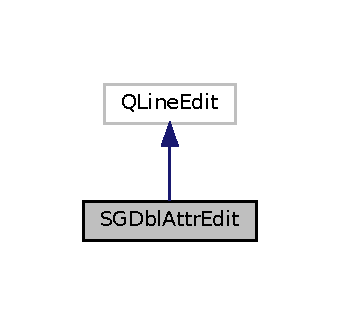
\includegraphics[width=163pt]{classSGDblAttrEdit__inherit__graph}
\end{center}
\end{figure}


Collaboration diagram for S\+G\+Dbl\+Attr\+Edit\+:
\nopagebreak
\begin{figure}[H]
\begin{center}
\leavevmode
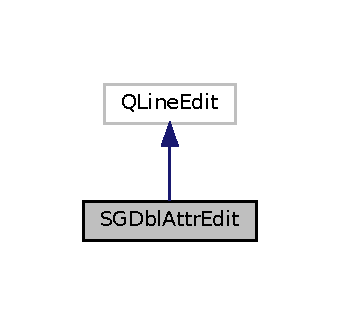
\includegraphics[width=163pt]{classSGDblAttrEdit__coll__graph}
\end{center}
\end{figure}
\subsection*{Public Member Functions}
\begin{DoxyCompactItemize}
\item 
\mbox{\Hypertarget{classSGDblAttrEdit_a4181190c83ed858568c41d9bdd4de5fd}\label{classSGDblAttrEdit_a4181190c83ed858568c41d9bdd4de5fd}} 
\hyperlink{classSGDblAttrEdit_a4181190c83ed858568c41d9bdd4de5fd}{S\+G\+Dbl\+Attr\+Edit} (double \&\+\_\+attr)
\begin{DoxyCompactList}\small\item\em Constructor. \end{DoxyCompactList}\end{DoxyCompactItemize}
\subsection*{Private Slots}
\begin{DoxyCompactItemize}
\item 
\mbox{\Hypertarget{classSGDblAttrEdit_a505bef38972a15a8537d3c4369f62f8d}\label{classSGDblAttrEdit_a505bef38972a15a8537d3c4369f62f8d}} 
void \hyperlink{classSGDblAttrEdit_a505bef38972a15a8537d3c4369f62f8d}{change\+Attr} (const Q\+String \&text)
\begin{DoxyCompactList}\small\item\em Slot called when Q\+Line\+Edit is edited. \end{DoxyCompactList}\end{DoxyCompactItemize}
\subsection*{Private Attributes}
\begin{DoxyCompactItemize}
\item 
\mbox{\Hypertarget{classSGDblAttrEdit_ad64b0b1fc2a05de5fc89d2d3dceeadf9}\label{classSGDblAttrEdit_ad64b0b1fc2a05de5fc89d2d3dceeadf9}} 
double \& \hyperlink{classSGDblAttrEdit_ad64b0b1fc2a05de5fc89d2d3dceeadf9}{attr}
\begin{DoxyCompactList}\small\item\em Reference to the attribute. \end{DoxyCompactList}\end{DoxyCompactItemize}


\subsection{Detailed Description}
A widget for editing double attributes. 

The documentation for this class was generated from the following file\+:\begin{DoxyCompactItemize}
\item 
viewer/hpp/sgrisksharinghandler.\+hpp\end{DoxyCompactItemize}

\hypertarget{classSGDblParamEdit}{}\section{S\+G\+Dbl\+Param\+Edit Class Reference}
\label{classSGDblParamEdit}\index{S\+G\+Dbl\+Param\+Edit@{S\+G\+Dbl\+Param\+Edit}}


Class for changing double parameters.  




{\ttfamily \#include $<$sgsettingshandler.\+hpp$>$}



Inheritance diagram for S\+G\+Dbl\+Param\+Edit\+:
\nopagebreak
\begin{figure}[H]
\begin{center}
\leavevmode
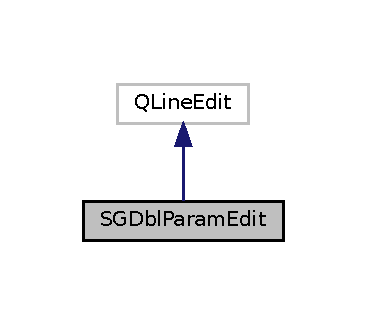
\includegraphics[width=176pt]{classSGDblParamEdit__inherit__graph}
\end{center}
\end{figure}


Collaboration diagram for S\+G\+Dbl\+Param\+Edit\+:
\nopagebreak
\begin{figure}[H]
\begin{center}
\leavevmode
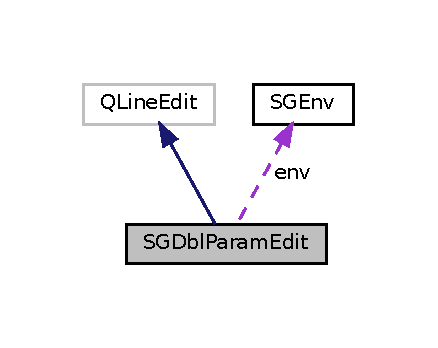
\includegraphics[width=210pt]{classSGDblParamEdit__coll__graph}
\end{center}
\end{figure}
\subsection*{Public Member Functions}
\begin{DoxyCompactItemize}
\item 
\mbox{\Hypertarget{classSGDblParamEdit_a04a6ff29f1494c926f07b34ca44ae75f}\label{classSGDblParamEdit_a04a6ff29f1494c926f07b34ca44ae75f}} 
\hyperlink{classSGDblParamEdit_a04a6ff29f1494c926f07b34ca44ae75f}{S\+G\+Dbl\+Param\+Edit} (Q\+Widget $\ast$parent, \hyperlink{classSGEnv}{S\+G\+Env} $\ast$\+\_\+env, \hyperlink{namespaceSG_ac2f86c953fcec4419ac86538d9d314b6}{S\+G\+::\+D\+B\+L\+\_\+\+P\+A\+R\+AM} \+\_\+param)
\begin{DoxyCompactList}\small\item\em Constructor. \end{DoxyCompactList}\end{DoxyCompactItemize}
\subsection*{Private Slots}
\begin{DoxyCompactItemize}
\item 
\mbox{\Hypertarget{classSGDblParamEdit_a1997b404f0484433f980c75e54c62e50}\label{classSGDblParamEdit_a1997b404f0484433f980c75e54c62e50}} 
void \hyperlink{classSGDblParamEdit_a1997b404f0484433f980c75e54c62e50}{change\+Param} (const Q\+String \&text)
\begin{DoxyCompactList}\small\item\em Slot called when the Q\+Line\+Edit is edited. \end{DoxyCompactList}\item 
\mbox{\Hypertarget{classSGDblParamEdit_a24f02d2e85467dd0883fbb055b3f00e1}\label{classSGDblParamEdit_a24f02d2e85467dd0883fbb055b3f00e1}} 
void \hyperlink{classSGDblParamEdit_a24f02d2e85467dd0883fbb055b3f00e1}{reset\+Param} ()
\begin{DoxyCompactList}\small\item\em Slot called when resetting to default values. \end{DoxyCompactList}\end{DoxyCompactItemize}
\subsection*{Private Attributes}
\begin{DoxyCompactItemize}
\item 
\mbox{\Hypertarget{classSGDblParamEdit_af4a14244a9b1a3f4e74da882b02f83f0}\label{classSGDblParamEdit_af4a14244a9b1a3f4e74da882b02f83f0}} 
\hyperlink{namespaceSG_ac2f86c953fcec4419ac86538d9d314b6}{S\+G\+::\+D\+B\+L\+\_\+\+P\+A\+R\+AM} \hyperlink{classSGDblParamEdit_af4a14244a9b1a3f4e74da882b02f83f0}{param}
\begin{DoxyCompactList}\small\item\em The double parameter associated with this edit. \end{DoxyCompactList}\item 
\mbox{\Hypertarget{classSGDblParamEdit_a4c9f7466833f32a1f8f3f4fc25def48c}\label{classSGDblParamEdit_a4c9f7466833f32a1f8f3f4fc25def48c}} 
\hyperlink{classSGEnv}{S\+G\+Env} $\ast$ \hyperlink{classSGDblParamEdit_a4c9f7466833f32a1f8f3f4fc25def48c}{env}
\begin{DoxyCompactList}\small\item\em The associated \hyperlink{classSGEnv}{S\+G\+Env} object. \end{DoxyCompactList}\end{DoxyCompactItemize}


\subsection{Detailed Description}
Class for changing double parameters. 

A customized version of Q\+Line\+Edit for modifying double parameters in an \hyperlink{classSGEnv}{S\+G\+Env} object that is used by the \hyperlink{classSGSettingsHandler}{S\+G\+Settings\+Handler}. It has a private members which are the particular \hyperlink{namespaceSG_ac2f86c953fcec4419ac86538d9d314b6}{S\+G\+::\+D\+B\+L\+\_\+\+P\+A\+R\+AM} that is associated with this edit and a pointer to an associated \hyperlink{classSGEnv}{S\+G\+Env} object. There are also mutator methods for setting the parameter value and resetting to the default value of the given parameter. 

The documentation for this class was generated from the following file\+:\begin{DoxyCompactItemize}
\item 
viewer/hpp/sgsettingshandler.\+hpp\end{DoxyCompactItemize}

\hypertarget{classSGEdgePolicy}{}\section{S\+G\+Edge\+Policy Class Reference}
\label{classSGEdgePolicy}\index{S\+G\+Edge\+Policy@{S\+G\+Edge\+Policy}}


Class for iterating edges of a product policy.  




{\ttfamily \#include $<$sgedgepolicy.\+hpp$>$}



Collaboration diagram for S\+G\+Edge\+Policy\+:
\nopagebreak
\begin{figure}[H]
\begin{center}
\leavevmode
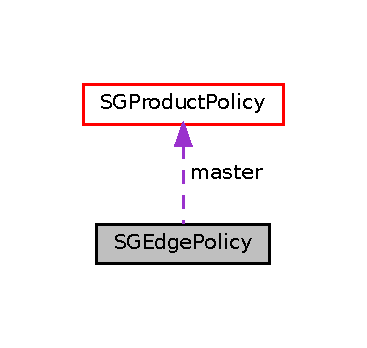
\includegraphics[width=176pt]{classSGEdgePolicy__coll__graph}
\end{center}
\end{figure}
\subsection*{Public Member Functions}
\begin{DoxyCompactItemize}
\item 
\hyperlink{classSGEdgePolicy_a72828530fdfd5e6d849dadd07ac44724}{S\+G\+Edge\+Policy} (const \hyperlink{classSGProductPolicy}{S\+G\+Product\+Policy} \&\+\_\+master)
\begin{DoxyCompactList}\small\item\em Constructor. \end{DoxyCompactList}\item 
\mbox{\Hypertarget{classSGEdgePolicy_abb6eb7cff5ea1a9f7007627cbc48a50c}\label{classSGEdgePolicy_abb6eb7cff5ea1a9f7007627cbc48a50c}} 
const vector$<$ S\+G\+Policy\+Set\+::const\+\_\+iterator $>$ \& \hyperlink{classSGEdgePolicy_abb6eb7cff5ea1a9f7007627cbc48a50c}{get\+Policies} () const
\begin{DoxyCompactList}\small\item\em Returns the current policy, as a vector of iterators. \end{DoxyCompactList}\item 
\mbox{\Hypertarget{classSGEdgePolicy_aa055206fa96e03f47547c1fcaaf7d19c}\label{classSGEdgePolicy_aa055206fa96e03f47547c1fcaaf7d19c}} 
const S\+G\+Policy\+Set\+::const\+\_\+iterator \& \hyperlink{classSGEdgePolicy_aa055206fa96e03f47547c1fcaaf7d19c}{get\+Sub\+Policy} () const
\begin{DoxyCompactList}\small\item\em Returns the current substitution. \end{DoxyCompactList}\item 
\mbox{\Hypertarget{classSGEdgePolicy_a967bd25525188460c0c4ab4881ed23f9}\label{classSGEdgePolicy_a967bd25525188460c0c4ab4881ed23f9}} 
bool \hyperlink{classSGEdgePolicy_a967bd25525188460c0c4ab4881ed23f9}{increment\+Base\+Policy} ()
\begin{DoxyCompactList}\small\item\em Increments the base policy. \end{DoxyCompactList}\item 
\mbox{\Hypertarget{classSGEdgePolicy_a07eb755f0281023ad7fc76190b33a83f}\label{classSGEdgePolicy_a07eb755f0281023ad7fc76190b33a83f}} 
bool \hyperlink{classSGEdgePolicy_a07eb755f0281023ad7fc76190b33a83f}{increment\+Sub\+Policy} ()
\begin{DoxyCompactList}\small\item\em Increments the substitution. \end{DoxyCompactList}\item 
\mbox{\Hypertarget{classSGEdgePolicy_a9ba9e008e8f581ed48b700ab51cc237a}\label{classSGEdgePolicy_a9ba9e008e8f581ed48b700ab51cc237a}} 
const int \hyperlink{classSGEdgePolicy_a9ba9e008e8f581ed48b700ab51cc237a}{get\+Base\+State} () const
\begin{DoxyCompactList}\small\item\em Returns the base state. \end{DoxyCompactList}\item 
\mbox{\Hypertarget{classSGEdgePolicy_a3e4ee651697b056738b6c8675b0c066d}\label{classSGEdgePolicy_a3e4ee651697b056738b6c8675b0c066d}} 
const int \hyperlink{classSGEdgePolicy_a3e4ee651697b056738b6c8675b0c066d}{get\+Sub\+State} () const
\begin{DoxyCompactList}\small\item\em Returns the substitution state. \end{DoxyCompactList}\item 
std\+::string \hyperlink{classSGEdgePolicy_ae106e1a7ebf78b0896316e16ca9c6063}{hash} () const
\begin{DoxyCompactList}\small\item\em Generates a unique identifier for the edge. \end{DoxyCompactList}\item 
\mbox{\Hypertarget{classSGEdgePolicy_a508ce3538972a16ecbaaff0362b785e2}\label{classSGEdgePolicy_a508ce3538972a16ecbaaff0362b785e2}} 
bool \hyperlink{classSGEdgePolicy_a508ce3538972a16ecbaaff0362b785e2}{operator++} ()
\begin{DoxyCompactList}\small\item\em Increment the edge by either advancing the substitution or the base policy. \end{DoxyCompactList}\end{DoxyCompactItemize}
\subsection*{Private Attributes}
\begin{DoxyCompactItemize}
\item 
const \hyperlink{classSGProductPolicy}{S\+G\+Product\+Policy} \& \hyperlink{classSGEdgePolicy_a78e0d811ff7c8847af1f84de160f8ec9}{master}
\item 
vector$<$ S\+G\+Policy\+Set\+::const\+\_\+iterator $>$ \hyperlink{classSGEdgePolicy_a4e18fb2c342c4349a89a2a47b5dc9f18}{policies}
\item 
S\+G\+Policy\+Set\+::const\+\_\+iterator \hyperlink{classSGEdgePolicy_a2b008e2ce91f6c95130af3efc5915e7f}{sub\+Policy}
\item 
int \hyperlink{classSGEdgePolicy_a28dccfb7e5195256e2ca6ababb03b45f}{base\+State}
\item 
int \hyperlink{classSGEdgePolicy_af12e8542627470a6c50abc6925512737}{sub\+State}
\end{DoxyCompactItemize}


\subsection{Detailed Description}
Class for iterating edges of a product policy. 

$<$ This code is used by \hyperlink{classSGSolver__MaxMinMax__3Player}{S\+G\+Solver\+\_\+\+Max\+Min\+Max\+\_\+3\+Player} for exact computation of the max-\/min-\/max operator when there are three players. Given a \char`\"{}master\char`\"{} product policy, which represents a face of $\tilde{B}({\bf W})$, this class will iterate through all edges of face. These edges correspond to (i) a selection of a policy in the product policy and (ii) a substitution. 

\subsection{Constructor \& Destructor Documentation}
\mbox{\Hypertarget{classSGEdgePolicy_a72828530fdfd5e6d849dadd07ac44724}\label{classSGEdgePolicy_a72828530fdfd5e6d849dadd07ac44724}} 
\index{S\+G\+Edge\+Policy@{S\+G\+Edge\+Policy}!S\+G\+Edge\+Policy@{S\+G\+Edge\+Policy}}
\index{S\+G\+Edge\+Policy@{S\+G\+Edge\+Policy}!S\+G\+Edge\+Policy@{S\+G\+Edge\+Policy}}
\subsubsection{\texorpdfstring{S\+G\+Edge\+Policy()}{SGEdgePolicy()}}
{\footnotesize\ttfamily S\+G\+Edge\+Policy\+::\+S\+G\+Edge\+Policy (\begin{DoxyParamCaption}\item[{const \hyperlink{classSGProductPolicy}{S\+G\+Product\+Policy} \&}]{\+\_\+master }\end{DoxyParamCaption})}



Constructor. 

Class for iterating edges of a product policy. 

\subsection{Member Function Documentation}
\mbox{\Hypertarget{classSGEdgePolicy_ae106e1a7ebf78b0896316e16ca9c6063}\label{classSGEdgePolicy_ae106e1a7ebf78b0896316e16ca9c6063}} 
\index{S\+G\+Edge\+Policy@{S\+G\+Edge\+Policy}!hash@{hash}}
\index{hash@{hash}!S\+G\+Edge\+Policy@{S\+G\+Edge\+Policy}}
\subsubsection{\texorpdfstring{hash()}{hash()}}
{\footnotesize\ttfamily std\+::string S\+G\+Edge\+Policy\+::hash (\begin{DoxyParamCaption}{ }\end{DoxyParamCaption}) const}



Generates a unique identifier for the edge. 

$<$ This identifier is used in tracking which edges have been visited. 

\subsection{Member Data Documentation}
\mbox{\Hypertarget{classSGEdgePolicy_a28dccfb7e5195256e2ca6ababb03b45f}\label{classSGEdgePolicy_a28dccfb7e5195256e2ca6ababb03b45f}} 
\index{S\+G\+Edge\+Policy@{S\+G\+Edge\+Policy}!base\+State@{base\+State}}
\index{base\+State@{base\+State}!S\+G\+Edge\+Policy@{S\+G\+Edge\+Policy}}
\subsubsection{\texorpdfstring{base\+State}{baseState}}
{\footnotesize\ttfamily int S\+G\+Edge\+Policy\+::base\+State\hspace{0.3cm}{\ttfamily [private]}}

The state in which we are currently iterating the policies, as we work our way through the product policy. \mbox{\Hypertarget{classSGEdgePolicy_a78e0d811ff7c8847af1f84de160f8ec9}\label{classSGEdgePolicy_a78e0d811ff7c8847af1f84de160f8ec9}} 
\index{S\+G\+Edge\+Policy@{S\+G\+Edge\+Policy}!master@{master}}
\index{master@{master}!S\+G\+Edge\+Policy@{S\+G\+Edge\+Policy}}
\subsubsection{\texorpdfstring{master}{master}}
{\footnotesize\ttfamily const \hyperlink{classSGProductPolicy}{S\+G\+Product\+Policy}\& S\+G\+Edge\+Policy\+::master\hspace{0.3cm}{\ttfamily [private]}}

The product policy describing the face. \mbox{\Hypertarget{classSGEdgePolicy_a4e18fb2c342c4349a89a2a47b5dc9f18}\label{classSGEdgePolicy_a4e18fb2c342c4349a89a2a47b5dc9f18}} 
\index{S\+G\+Edge\+Policy@{S\+G\+Edge\+Policy}!policies@{policies}}
\index{policies@{policies}!S\+G\+Edge\+Policy@{S\+G\+Edge\+Policy}}
\subsubsection{\texorpdfstring{policies}{policies}}
{\footnotesize\ttfamily vector$<$S\+G\+Policy\+Set\+::const\+\_\+iterator$>$ S\+G\+Edge\+Policy\+::policies\hspace{0.3cm}{\ttfamily [private]}}

The vector of policies that makes up the current edge. \mbox{\Hypertarget{classSGEdgePolicy_a2b008e2ce91f6c95130af3efc5915e7f}\label{classSGEdgePolicy_a2b008e2ce91f6c95130af3efc5915e7f}} 
\index{S\+G\+Edge\+Policy@{S\+G\+Edge\+Policy}!sub\+Policy@{sub\+Policy}}
\index{sub\+Policy@{sub\+Policy}!S\+G\+Edge\+Policy@{S\+G\+Edge\+Policy}}
\subsubsection{\texorpdfstring{sub\+Policy}{subPolicy}}
{\footnotesize\ttfamily S\+G\+Policy\+Set\+::const\+\_\+iterator S\+G\+Edge\+Policy\+::sub\+Policy\hspace{0.3cm}{\ttfamily [private]}}

The substituted policy. \mbox{\Hypertarget{classSGEdgePolicy_af12e8542627470a6c50abc6925512737}\label{classSGEdgePolicy_af12e8542627470a6c50abc6925512737}} 
\index{S\+G\+Edge\+Policy@{S\+G\+Edge\+Policy}!sub\+State@{sub\+State}}
\index{sub\+State@{sub\+State}!S\+G\+Edge\+Policy@{S\+G\+Edge\+Policy}}
\subsubsection{\texorpdfstring{sub\+State}{subState}}
{\footnotesize\ttfamily int S\+G\+Edge\+Policy\+::sub\+State\hspace{0.3cm}{\ttfamily [private]}}

State in which the policy is substituted. 

The documentation for this class was generated from the following files\+:\begin{DoxyCompactItemize}
\item 
src/hpp/sgedgepolicy.\+hpp\item 
src/cpp/sgedgepolicy.\+cpp\end{DoxyCompactItemize}

\hypertarget{classSGEnv}{}\section{S\+G\+Env Class Reference}
\label{classSGEnv}\index{S\+G\+Env@{S\+G\+Env}}


Manages parameters for algorithm behavior.  




{\ttfamily \#include $<$sgenv.\+hpp$>$}

\subsection*{Public Member Functions}
\begin{DoxyCompactItemize}
\item 
\hyperlink{classSGEnv_ac7fe265f0baba4e498c36bd67a0bbc97}{S\+G\+Env} ()
\begin{DoxyCompactList}\small\item\em Constructor. \end{DoxyCompactList}\item 
\mbox{\Hypertarget{classSGEnv_adfa101d39534519c80b33a78454b01e2}\label{classSGEnv_adfa101d39534519c80b33a78454b01e2}} 
void \hyperlink{classSGEnv_adfa101d39534519c80b33a78454b01e2}{set\+Param} (\hyperlink{namespaceSG_ac2f86c953fcec4419ac86538d9d314b6}{S\+G\+::\+D\+B\+L\+\_\+\+P\+A\+R\+AM} param, double value)
\begin{DoxyCompactList}\small\item\em Method for setting double parameters. \end{DoxyCompactList}\item 
\mbox{\Hypertarget{classSGEnv_a94d5a63cc1023e86e239b203c86dca8d}\label{classSGEnv_a94d5a63cc1023e86e239b203c86dca8d}} 
void \hyperlink{classSGEnv_a94d5a63cc1023e86e239b203c86dca8d}{set\+Param} (\hyperlink{namespaceSG_a0b164afe6c58be3386d9e3f6e857b673}{S\+G\+::\+B\+O\+O\+L\+\_\+\+P\+A\+R\+AM} param, bool value)
\begin{DoxyCompactList}\small\item\em Method for setting boolean parameters. \end{DoxyCompactList}\item 
\mbox{\Hypertarget{classSGEnv_ab34537d887371f2f1e1af3d13f2c0d0a}\label{classSGEnv_ab34537d887371f2f1e1af3d13f2c0d0a}} 
void \hyperlink{classSGEnv_ab34537d887371f2f1e1af3d13f2c0d0a}{set\+Param} (\hyperlink{namespaceSG_a031898e6fc0fa14d8590f85da9715f37}{S\+G\+::\+I\+N\+T\+\_\+\+P\+A\+R\+AM} param, int value)
\begin{DoxyCompactList}\small\item\em Method for setting integer parameters. \end{DoxyCompactList}\item 
\mbox{\Hypertarget{classSGEnv_ae3b508ceaf8d9aec513dde852ba67579}\label{classSGEnv_ae3b508ceaf8d9aec513dde852ba67579}} 
double \hyperlink{classSGEnv_ae3b508ceaf8d9aec513dde852ba67579}{get\+Param} (\hyperlink{namespaceSG_ac2f86c953fcec4419ac86538d9d314b6}{S\+G\+::\+D\+B\+L\+\_\+\+P\+A\+R\+AM} param) const
\begin{DoxyCompactList}\small\item\em Method for getting double parameters. \end{DoxyCompactList}\item 
\mbox{\Hypertarget{classSGEnv_a13c98e1199f9a26375b525276650f954}\label{classSGEnv_a13c98e1199f9a26375b525276650f954}} 
bool \hyperlink{classSGEnv_a13c98e1199f9a26375b525276650f954}{get\+Param} (\hyperlink{namespaceSG_a0b164afe6c58be3386d9e3f6e857b673}{S\+G\+::\+B\+O\+O\+L\+\_\+\+P\+A\+R\+AM} param) const
\begin{DoxyCompactList}\small\item\em Method for getting boolean parameters. \end{DoxyCompactList}\item 
\mbox{\Hypertarget{classSGEnv_abf98a7ee14af5678e72577cdbc2d6fd3}\label{classSGEnv_abf98a7ee14af5678e72577cdbc2d6fd3}} 
int \hyperlink{classSGEnv_abf98a7ee14af5678e72577cdbc2d6fd3}{get\+Param} (\hyperlink{namespaceSG_a031898e6fc0fa14d8590f85da9715f37}{S\+G\+::\+I\+N\+T\+\_\+\+P\+A\+R\+AM} param) const
\begin{DoxyCompactList}\small\item\em Method for getting integer parameters. \end{DoxyCompactList}\item 
\mbox{\Hypertarget{classSGEnv_a77e0bf7bafe7b9d6da890ccd6d1db624}\label{classSGEnv_a77e0bf7bafe7b9d6da890ccd6d1db624}} 
void \hyperlink{classSGEnv_a77e0bf7bafe7b9d6da890ccd6d1db624}{restore\+Defaults} ()
\begin{DoxyCompactList}\small\item\em Method for restoring default values for all parameters. \end{DoxyCompactList}\item 
\mbox{\Hypertarget{classSGEnv_abc39cb53702f831728fa577be5f09b97}\label{classSGEnv_abc39cb53702f831728fa577be5f09b97}} 
{\footnotesize template$<$class Archive $>$ }\\void \hyperlink{classSGEnv_abc39cb53702f831728fa577be5f09b97}{serialize} (Archive \&ar, const unsigned int version)
\begin{DoxyCompactList}\small\item\em Serializes the action using the boost\+::serialization library. \end{DoxyCompactList}\end{DoxyCompactItemize}
\subsection*{Private Attributes}
\begin{DoxyCompactItemize}
\item 
\mbox{\Hypertarget{classSGEnv_af5b5de418e3c1a84ee8a6af8ac4e4b9b}\label{classSGEnv_af5b5de418e3c1a84ee8a6af8ac4e4b9b}} 
vector$<$ double $>$ \hyperlink{classSGEnv_af5b5de418e3c1a84ee8a6af8ac4e4b9b}{double\+Params}
\begin{DoxyCompactList}\small\item\em Double parameters. \end{DoxyCompactList}\item 
\mbox{\Hypertarget{classSGEnv_a2a4034a806454ea25a88f2fcf9610c50}\label{classSGEnv_a2a4034a806454ea25a88f2fcf9610c50}} 
vector$<$ bool $>$ \hyperlink{classSGEnv_a2a4034a806454ea25a88f2fcf9610c50}{bool\+Params}
\begin{DoxyCompactList}\small\item\em Bool parameters. \end{DoxyCompactList}\item 
\mbox{\Hypertarget{classSGEnv_a2b0bb12821ee9147615be6e887f93ed1}\label{classSGEnv_a2b0bb12821ee9147615be6e887f93ed1}} 
vector$<$ int $>$ \hyperlink{classSGEnv_a2b0bb12821ee9147615be6e887f93ed1}{int\+Params}
\begin{DoxyCompactList}\small\item\em Int parameters. \end{DoxyCompactList}\end{DoxyCompactItemize}


\subsection{Detailed Description}
Manages parameters for algorithm behavior. 

This class contains parameters for the algorithm.

T\+O\+DO\+: Add more checks on the correctness of passed parameter values. \begin{Desc}
\item[Examples\+: ]\par
\hyperlink{pd_twostate_8cpp-example}{pd\+\_\+twostate.\+cpp}, and \hyperlink{risksharing_maxminmax_8cpp-example}{risksharing\+\_\+maxminmax.\+cpp}.\end{Desc}


\subsection{Constructor \& Destructor Documentation}
\mbox{\Hypertarget{classSGEnv_ac7fe265f0baba4e498c36bd67a0bbc97}\label{classSGEnv_ac7fe265f0baba4e498c36bd67a0bbc97}} 
\index{S\+G\+Env@{S\+G\+Env}!S\+G\+Env@{S\+G\+Env}}
\index{S\+G\+Env@{S\+G\+Env}!S\+G\+Env@{S\+G\+Env}}
\subsubsection{\texorpdfstring{S\+G\+Env()}{SGEnv()}}
{\footnotesize\ttfamily S\+G\+Env\+::\+S\+G\+Env (\begin{DoxyParamCaption}{ }\end{DoxyParamCaption})}



Constructor. 

Creates a new \hyperlink{classSGEnv}{S\+G\+Env} object and initializes with default parameter values. 

The documentation for this class was generated from the following files\+:\begin{DoxyCompactItemize}
\item 
src/hpp/sgenv.\+hpp\item 
src/cpp/sgenv.\+cpp\end{DoxyCompactItemize}

\hypertarget{classSGException}{}\section{S\+G\+Exception Class Reference}
\label{classSGException}\index{S\+G\+Exception@{S\+G\+Exception}}


S\+G\+Solve specific exceptions.  




{\ttfamily \#include $<$sgexception.\+hpp$>$}



Inheritance diagram for S\+G\+Exception\+:
\nopagebreak
\begin{figure}[H]
\begin{center}
\leavevmode
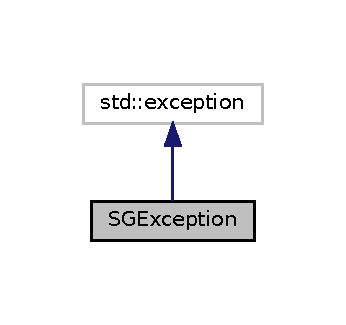
\includegraphics[width=166pt]{classSGException__inherit__graph}
\end{center}
\end{figure}


Collaboration diagram for S\+G\+Exception\+:
\nopagebreak
\begin{figure}[H]
\begin{center}
\leavevmode
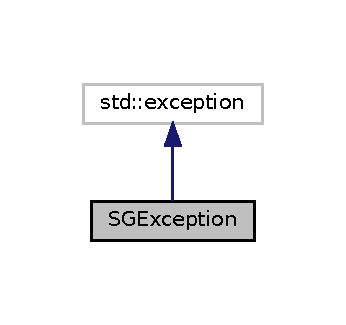
\includegraphics[width=166pt]{classSGException__coll__graph}
\end{center}
\end{figure}
\subsection*{Public Member Functions}
\begin{DoxyCompactItemize}
\item 
\mbox{\Hypertarget{classSGException_a45a1ee37ef4e6d20c9711ee417009889}\label{classSGException_a45a1ee37ef4e6d20c9711ee417009889}} 
\hyperlink{classSGException_a45a1ee37ef4e6d20c9711ee417009889}{S\+G\+Exception} (\hyperlink{namespaceSG_a671df7c720746d1e853deee02bad6411}{S\+G\+::\+E\+X\+C\+E\+P\+T\+I\+O\+N\+\_\+\+T\+Y\+PE} \+\_\+type=\hyperlink{namespaceSG_a671df7c720746d1e853deee02bad6411a0c0f6f82ce3e38637b36fdf4fe34d79f}{S\+G\+::\+D\+E\+F\+A\+U\+LT})
\begin{DoxyCompactList}\small\item\em Constructor for new \hyperlink{classSGException}{S\+G\+Exception}. \end{DoxyCompactList}\item 
\mbox{\Hypertarget{classSGException_a5a43e290f591ee26d0674d3455f6c144}\label{classSGException_a5a43e290f591ee26d0674d3455f6c144}} 
virtual const char $\ast$ \hyperlink{classSGException_a5a43e290f591ee26d0674d3455f6c144}{what} () const  throw ()
\begin{DoxyCompactList}\small\item\em Returns the message corresponding to the Exception\+Type. \end{DoxyCompactList}\item 
\mbox{\Hypertarget{classSGException_afd64ecf52ffdf1b2f8c20103a73cbc60}\label{classSGException_afd64ecf52ffdf1b2f8c20103a73cbc60}} 
\hyperlink{namespaceSG_a671df7c720746d1e853deee02bad6411}{S\+G\+::\+E\+X\+C\+E\+P\+T\+I\+O\+N\+\_\+\+T\+Y\+PE} \hyperlink{classSGException_afd64ecf52ffdf1b2f8c20103a73cbc60}{get\+Type} () const
\begin{DoxyCompactList}\small\item\em Returns the type of the exception. \end{DoxyCompactList}\end{DoxyCompactItemize}
\subsection*{Private Attributes}
\begin{DoxyCompactItemize}
\item 
\mbox{\Hypertarget{classSGException_aa010288cdfd8ff0ef068b23c614601b6}\label{classSGException_aa010288cdfd8ff0ef068b23c614601b6}} 
\hyperlink{namespaceSG_a671df7c720746d1e853deee02bad6411}{S\+G\+::\+E\+X\+C\+E\+P\+T\+I\+O\+N\+\_\+\+T\+Y\+PE} \hyperlink{classSGException_aa010288cdfd8ff0ef068b23c614601b6}{type}
\begin{DoxyCompactList}\small\item\em Flag that indicates the type of error encountered. \end{DoxyCompactList}\end{DoxyCompactItemize}


\subsection{Detailed Description}
S\+G\+Solve specific exceptions. 

This class is derived from std\+::exception and handles special messages that are informative about abnormal behavior in \hyperlink{classSGSolver}{S\+G\+Solver} and associated classes. \begin{Desc}
\item[Examples\+: ]\par
\hyperlink{pd_twostate_8cpp-example}{pd\+\_\+twostate.\+cpp}.\end{Desc}


The documentation for this class was generated from the following files\+:\begin{DoxyCompactItemize}
\item 
src/hpp/sgexception.\+hpp\item 
src/cpp/sgexception.\+cpp\end{DoxyCompactItemize}

\hypertarget{classSGGame}{}\section{S\+G\+Game Class Reference}
\label{classSGGame}\index{S\+G\+Game@{S\+G\+Game}}


Describes a stochastic game.  




{\ttfamily \#include $<$sggame.\+hpp$>$}



Collaboration diagram for S\+G\+Game\+:
\nopagebreak
\begin{figure}[H]
\begin{center}
\leavevmode
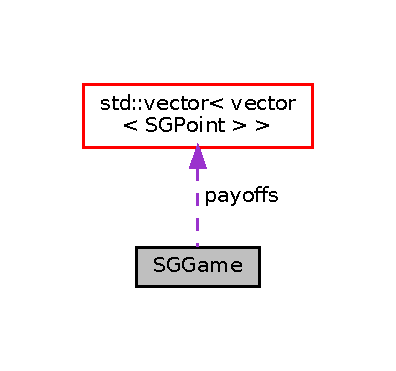
\includegraphics[width=190pt]{classSGGame__coll__graph}
\end{center}
\end{figure}
\subsection*{Public Member Functions}
\begin{DoxyCompactItemize}
\item 
\mbox{\Hypertarget{classSGGame_a935fc76700c675f842dc1666ffe2e8f7}\label{classSGGame_a935fc76700c675f842dc1666ffe2e8f7}} 
\hyperlink{classSGGame_a935fc76700c675f842dc1666ffe2e8f7}{S\+G\+Game} ()
\begin{DoxyCompactList}\small\item\em Default constructor. \end{DoxyCompactList}\item 
\hyperlink{classSGGame_a0b85bb1b3a04539bef72dadc7e170b2f}{S\+G\+Game} (const \hyperlink{classSGAbstractGame}{S\+G\+Abstract\+Game} \&game)
\begin{DoxyCompactList}\small\item\em Converts an \hyperlink{classSGAbstractGame}{S\+G\+Abstract\+Game} into a \hyperlink{classSGGame}{S\+G\+Game}. \end{DoxyCompactList}\item 
\hyperlink{classSGGame_ad881fb3f3db38d4b7c2ea0beb7181fc0}{S\+G\+Game} (double \+\_\+delta, int \+\_\+num\+States, const vector$<$ vector$<$ int $>$ $>$ \&\+\_\+num\+Actions, const vector$<$ vector$<$ vector$<$ double $>$ $>$ $>$ \&\+\_\+payoffs, const vector$<$ vector$<$ vector$<$ double $>$ $>$ $>$ \&\+\_\+probabilities)
\begin{DoxyCompactList}\small\item\em Constructor excluding eq\+Actions. \end{DoxyCompactList}\item 
\mbox{\Hypertarget{classSGGame_ad4d48551202bda3c56f8860a24f04260}\label{classSGGame_ad4d48551202bda3c56f8860a24f04260}} 
\hyperlink{classSGGame_ad4d48551202bda3c56f8860a24f04260}{S\+G\+Game} (double \+\_\+delta, int \+\_\+num\+States, const vector$<$ vector$<$ int $>$ $>$ \&\+\_\+num\+Actions, const vector$<$ vector$<$ vector$<$ double $>$ $>$ $>$ \&\+\_\+payoffs, const vector$<$ vector$<$ vector$<$ double $>$ $>$ $>$ \&\+\_\+probabilities, const vector$<$ bool $>$ \&\+\_\+unconstrained)
\begin{DoxyCompactList}\small\item\em Constructor customizing unconstrained. \end{DoxyCompactList}\item 
\hyperlink{classSGGame_abf23f0bd27cc79e44bdae273ef8a7735}{S\+G\+Game} (double \+\_\+delta, int \+\_\+num\+States, const vector$<$ vector$<$ int $>$ $>$ \&\+\_\+num\+Actions, const vector$<$ vector$<$ vector$<$ double $>$ $>$ $>$ \&\+\_\+payoffs, const vector$<$ vector$<$ vector$<$ double $>$ $>$ $>$ \&\+\_\+probabilities, const vector$<$ vector$<$ bool $>$ $>$ \&\+\_\+eq\+Actions, const vector$<$ bool $>$ \&\+\_\+unconstrained)
\begin{DoxyCompactList}\small\item\em Constructor customizing equilibrium actions. \end{DoxyCompactList}\item 
\hyperlink{classSGGame_af6715eb62a0133849bbe9fe60fe113ab}{S\+G\+Game} (int \+\_\+num\+Players, double \+\_\+delta, int \+\_\+num\+States, const vector$<$ vector$<$ int $>$ $>$ \&\+\_\+num\+Actions, const vector$<$ vector$<$ vector$<$ double $>$ $>$ $>$ \&\+\_\+payoffs, const vector$<$ vector$<$ vector$<$ double $>$ $>$ $>$ \&\+\_\+probabilities, const vector$<$ vector$<$ bool $>$ $>$ \&\+\_\+eq\+Actions, const vector$<$ bool $>$ \&\+\_\+unconstrained)
\begin{DoxyCompactList}\small\item\em Constructor with custom num\+Players. \end{DoxyCompactList}\item 
\mbox{\Hypertarget{classSGGame_aefa61117ee6c117c297791f976b36324}\label{classSGGame_aefa61117ee6c117c297791f976b36324}} 
double \hyperlink{classSGGame_aefa61117ee6c117c297791f976b36324}{get\+Delta} () const
\begin{DoxyCompactList}\small\item\em Returns \hyperlink{classSGGame_a5031fc31f8009c19901c0930224e0465}{S\+G\+Game\+::delta}, the discount factor. \end{DoxyCompactList}\item 
\mbox{\Hypertarget{classSGGame_aaecc5512e85b0c360d4c462d3f84eae0}\label{classSGGame_aaecc5512e85b0c360d4c462d3f84eae0}} 
int \hyperlink{classSGGame_aaecc5512e85b0c360d4c462d3f84eae0}{get\+Num\+Players} () const
\begin{DoxyCompactList}\small\item\em Returns \hyperlink{classSGGame_a6f02e3f92db6a3c5d2d9076dcb7b6d61}{S\+G\+Game\+::num\+Players}, the number of players. \end{DoxyCompactList}\item 
\mbox{\Hypertarget{classSGGame_a1cbb93f4557f71df9d7bffcfeb8ff51c}\label{classSGGame_a1cbb93f4557f71df9d7bffcfeb8ff51c}} 
int \hyperlink{classSGGame_a1cbb93f4557f71df9d7bffcfeb8ff51c}{get\+Num\+States} () const
\begin{DoxyCompactList}\small\item\em Returns the number of states. \end{DoxyCompactList}\item 
\mbox{\Hypertarget{classSGGame_acfd5f0817645a9adf9474552aca4f62e}\label{classSGGame_acfd5f0817645a9adf9474552aca4f62e}} 
const vector$<$ vector$<$ int $>$ $>$ \& \hyperlink{classSGGame_acfd5f0817645a9adf9474552aca4f62e}{get\+Num\+Actions} () const
\begin{DoxyCompactList}\small\item\em Sets the argument \+\_\+num\+Actions equal to \hyperlink{classSGGame_acebe94d195ffb67f92925bcd4c26d1a9}{S\+G\+Game\+::num\+Actions}. \end{DoxyCompactList}\item 
const vector$<$ int $>$ \& \hyperlink{classSGGame_a22f9effebebb711e2f174c4a95a49420}{get\+Num\+Actions\+\_\+total} () const
\item 
\mbox{\Hypertarget{classSGGame_a0d2fef107bd38ad4c848fd35b0ed5ddf}\label{classSGGame_a0d2fef107bd38ad4c848fd35b0ed5ddf}} 
const vector$<$ vector$<$ vector$<$ double $>$ $>$ $>$ \& \hyperlink{classSGGame_a0d2fef107bd38ad4c848fd35b0ed5ddf}{get\+Probabilities} () const
\begin{DoxyCompactList}\small\item\em Returns a const reference to probabilities. \end{DoxyCompactList}\item 
\mbox{\Hypertarget{classSGGame_a37036f4f8389a68c53b12eb75c1eb7af}\label{classSGGame_a37036f4f8389a68c53b12eb75c1eb7af}} 
const vector$<$ vector$<$ \hyperlink{classSGPoint}{S\+G\+Point} $>$ $>$ \& \hyperlink{classSGGame_a37036f4f8389a68c53b12eb75c1eb7af}{get\+Payoffs} () const
\begin{DoxyCompactList}\small\item\em Returns a const reference to the payoffs. \end{DoxyCompactList}\item 
\mbox{\Hypertarget{classSGGame_a5cbb8386739f0ddcb6bc1666dcba3b7b}\label{classSGGame_a5cbb8386739f0ddcb6bc1666dcba3b7b}} 
const vector$<$ vector$<$ bool $>$ $>$ \& \hyperlink{classSGGame_a5cbb8386739f0ddcb6bc1666dcba3b7b}{get\+Equilibrium\+Actions} () const
\begin{DoxyCompactList}\small\item\em Returns a const reference to the equilibrium actions. \end{DoxyCompactList}\item 
void \hyperlink{classSGGame_a32293b2ba26d2a8cd264e3b9e7559d22}{get\+Payoff\+Bounds} (\hyperlink{classSGPoint}{S\+G\+Point} \&UB, \hyperlink{classSGPoint}{S\+G\+Point} \&LB) const
\item 
\mbox{\Hypertarget{classSGGame_aa32846060a1f8a9b9fc0419a1c1c0510}\label{classSGGame_aa32846060a1f8a9b9fc0419a1c1c0510}} 
const vector$<$ bool $>$ \& \hyperlink{classSGGame_aa32846060a1f8a9b9fc0419a1c1c0510}{get\+Constrained} () const
\begin{DoxyCompactList}\small\item\em Returns the unconstrained vector. \end{DoxyCompactList}\item 
bool \hyperlink{classSGGame_ad5879878c647da7040940469b56b9595}{set\+Discount\+Factor} (double new\+Delta)
\begin{DoxyCompactList}\small\item\em Set discount factor. \end{DoxyCompactList}\item 
bool \hyperlink{classSGGame_a36b2269c87d27ab3e0278ad44b6bbddc}{set\+Payoff} (int state, int action, int player, double payoff)
\begin{DoxyCompactList}\small\item\em Set payoffs. \end{DoxyCompactList}\item 
bool \hyperlink{classSGGame_afcc31eacca8f294d349905d52c9a5f64}{set\+Probability} (int state, int action, int new\+State, double prob)
\begin{DoxyCompactList}\small\item\em Set probability. \end{DoxyCompactList}\item 
\mbox{\Hypertarget{classSGGame_a5526a6eb4c4fbb9bc6ff3334e411fbf1}\label{classSGGame_a5526a6eb4c4fbb9bc6ff3334e411fbf1}} 
bool \hyperlink{classSGGame_a5526a6eb4c4fbb9bc6ff3334e411fbf1}{set\+Constrained} (const vector$<$ bool $>$ \&\+\_\+unconstrained)
\begin{DoxyCompactList}\small\item\em Sets whether or not players are incentive constrained. \end{DoxyCompactList}\item 
bool \hyperlink{classSGGame_a2b3ddf3f5dfca8514cba1933205c5ec3}{add\+Action} (int state, int player, int position)
\begin{DoxyCompactList}\small\item\em Adds a new action. \end{DoxyCompactList}\item 
\mbox{\Hypertarget{classSGGame_a97999290a05ab0427fd36d0a2a737944}\label{classSGGame_a97999290a05ab0427fd36d0a2a737944}} 
bool \hyperlink{classSGGame_a97999290a05ab0427fd36d0a2a737944}{remove\+Action} (int state, int player, int action)
\begin{DoxyCompactList}\small\item\em Removes the given action. \end{DoxyCompactList}\item 
bool \hyperlink{classSGGame_a0e4ea56b9e9787dca697782cbedc76d6}{add\+State} (int position)
\begin{DoxyCompactList}\small\item\em Adds a new state. \end{DoxyCompactList}\item 
\mbox{\Hypertarget{classSGGame_ae4930c4311ee2f7a814400e3e50123a8}\label{classSGGame_ae4930c4311ee2f7a814400e3e50123a8}} 
bool \hyperlink{classSGGame_ae4930c4311ee2f7a814400e3e50123a8}{remove\+State} (int state)
\begin{DoxyCompactList}\small\item\em Removes the given state. \end{DoxyCompactList}\item 
\mbox{\Hypertarget{classSGGame_a4bf2a75864749594145cbd2194ebadd4}\label{classSGGame_a4bf2a75864749594145cbd2194ebadd4}} 
bool \hyperlink{classSGGame_a4bf2a75864749594145cbd2194ebadd4}{transition\+Probs\+Sum\+To\+One} () const
\begin{DoxyCompactList}\small\item\em Check if transition probabilities sum to one. \end{DoxyCompactList}\end{DoxyCompactItemize}
\subsection*{Static Public Member Functions}
\begin{DoxyCompactItemize}
\item 
\mbox{\Hypertarget{classSGGame_aaccf18a3663ec99360e5b6e64f2bf6e2}\label{classSGGame_aaccf18a3663ec99360e5b6e64f2bf6e2}} 
static void \hyperlink{classSGGame_aaccf18a3663ec99360e5b6e64f2bf6e2}{save} (const \hyperlink{classSGGame}{S\+G\+Game} \&game, const char $\ast$filename)
\begin{DoxyCompactList}\small\item\em Static method for saving an \hyperlink{classSGGame}{S\+G\+Game} object to the file filename. \end{DoxyCompactList}\item 
\mbox{\Hypertarget{classSGGame_ac1dc35b84318448efc37b80afe210170}\label{classSGGame_ac1dc35b84318448efc37b80afe210170}} 
static void \hyperlink{classSGGame_ac1dc35b84318448efc37b80afe210170}{load} (\hyperlink{classSGGame}{S\+G\+Game} \&game, const char $\ast$filename)
\begin{DoxyCompactList}\small\item\em Static method for loading an \hyperlink{classSGGame}{S\+G\+Game} object from the file filename. \end{DoxyCompactList}\end{DoxyCompactItemize}
\subsection*{Private Member Functions}
\begin{DoxyCompactItemize}
\item 
\mbox{\Hypertarget{classSGGame_a383c8f7ec881befac40d6e45c7e1b775}\label{classSGGame_a383c8f7ec881befac40d6e45c7e1b775}} 
{\footnotesize template$<$class Archive $>$ }\\void \hyperlink{classSGGame_a383c8f7ec881befac40d6e45c7e1b775}{serialize} (Archive \&ar, const unsigned int version)
\begin{DoxyCompactList}\small\item\em Serializes the game using boost. \end{DoxyCompactList}\end{DoxyCompactItemize}
\subsection*{Private Attributes}
\begin{DoxyCompactItemize}
\item 
double \hyperlink{classSGGame_a5031fc31f8009c19901c0930224e0465}{delta}
\item 
int \hyperlink{classSGGame_a6f02e3f92db6a3c5d2d9076dcb7b6d61}{num\+Players}
\item 
int \hyperlink{classSGGame_ae7b105b2fe9ee277d38e518223dd0482}{num\+States}
\item 
vector$<$ vector$<$ int $>$ $>$ \hyperlink{classSGGame_acebe94d195ffb67f92925bcd4c26d1a9}{num\+Actions}
\item 
vector$<$ int $>$ \hyperlink{classSGGame_a3b219a37177b5b8b38737f570e419429}{num\+Actions\+\_\+total}
\item 
vector$<$ vector$<$ \hyperlink{classSGPoint}{S\+G\+Point} $>$ $>$ \hyperlink{classSGGame_aad28dd39c6359e772286a938a948634c}{payoffs}
\item 
vector$<$ vector$<$ vector$<$ double $>$ $>$ $>$ \hyperlink{classSGGame_a167a281b11d524cb4a11dbaff3e9de68}{probabilities}
\item 
vector$<$ vector$<$ bool $>$ $>$ \hyperlink{classSGGame_aacb0878b1e95ef3ff42cb88ac617c0b8}{eq\+Actions}
\item 
vector$<$ bool $>$ \hyperlink{classSGGame_a528852e11bd68322535d7f24a41eca20}{unconstrained}
\end{DoxyCompactItemize}
\subsection*{Friends}
\begin{DoxyCompactItemize}
\item 
\mbox{\Hypertarget{classSGGame_ac98d07dd8f7b70e16ccb9a01abf56b9c}\label{classSGGame_ac98d07dd8f7b70e16ccb9a01abf56b9c}} 
class {\bfseries boost\+::serialization\+::access}
\item 
\mbox{\Hypertarget{classSGGame_a8b0e5d2bebfed7e7e032366bb49bc5f1}\label{classSGGame_a8b0e5d2bebfed7e7e032366bb49bc5f1}} 
class {\bfseries S\+G\+Solver}
\end{DoxyCompactItemize}


\subsection{Detailed Description}
Describes a stochastic game. 

This class contains members that describe a stochastic game. \begin{Desc}
\item[Examples\+: ]\par
\hyperlink{pd_twostate_8cpp-example}{pd\+\_\+twostate.\+cpp}, and \hyperlink{risksharing_maxminmax_8cpp-example}{risksharing\+\_\+maxminmax.\+cpp}.\end{Desc}


\subsection{Constructor \& Destructor Documentation}
\mbox{\Hypertarget{classSGGame_a0b85bb1b3a04539bef72dadc7e170b2f}\label{classSGGame_a0b85bb1b3a04539bef72dadc7e170b2f}} 
\index{S\+G\+Game@{S\+G\+Game}!S\+G\+Game@{S\+G\+Game}}
\index{S\+G\+Game@{S\+G\+Game}!S\+G\+Game@{S\+G\+Game}}
\subsubsection{\texorpdfstring{S\+G\+Game()}{SGGame()}\hspace{0.1cm}{\footnotesize\ttfamily [1/4]}}
{\footnotesize\ttfamily S\+G\+Game\+::\+S\+G\+Game (\begin{DoxyParamCaption}\item[{const \hyperlink{classSGAbstractGame}{S\+G\+Abstract\+Game} \&}]{game }\end{DoxyParamCaption})}



Converts an \hyperlink{classSGAbstractGame}{S\+G\+Abstract\+Game} into a \hyperlink{classSGGame}{S\+G\+Game}. 

The user can derive their own class from \hyperlink{classSGAbstractGame}{S\+G\+Abstract\+Game}, and then pass the derived object to the \hyperlink{classSGGame}{S\+G\+Game} constructor. This constructor essentially copies the data from the user defined payoffs and probability methods into arrays. Storing this data in arrays provides for faster access by \hyperlink{classSGApprox}{S\+G\+Approx} and it allows the game to be serialized. See risksharing.\+hpp and risksharing.\+cpp for an example. \mbox{\Hypertarget{classSGGame_ad881fb3f3db38d4b7c2ea0beb7181fc0}\label{classSGGame_ad881fb3f3db38d4b7c2ea0beb7181fc0}} 
\index{S\+G\+Game@{S\+G\+Game}!S\+G\+Game@{S\+G\+Game}}
\index{S\+G\+Game@{S\+G\+Game}!S\+G\+Game@{S\+G\+Game}}
\subsubsection{\texorpdfstring{S\+G\+Game()}{SGGame()}\hspace{0.1cm}{\footnotesize\ttfamily [2/4]}}
{\footnotesize\ttfamily S\+G\+Game\+::\+S\+G\+Game (\begin{DoxyParamCaption}\item[{double}]{\+\_\+delta,  }\item[{int}]{\+\_\+num\+States,  }\item[{const vector$<$ vector$<$ int $>$ $>$ \&}]{\+\_\+num\+Actions,  }\item[{const vector$<$ vector$<$ vector$<$ double $>$ $>$ $>$ \&}]{\+\_\+payoffs,  }\item[{const vector$<$ vector$<$ vector$<$ double $>$ $>$ $>$ \&}]{\+\_\+probabilities }\end{DoxyParamCaption})}



Constructor excluding eq\+Actions. 

$<$ Initializes a game object with all actions being permissible. \mbox{\Hypertarget{classSGGame_abf23f0bd27cc79e44bdae273ef8a7735}\label{classSGGame_abf23f0bd27cc79e44bdae273ef8a7735}} 
\index{S\+G\+Game@{S\+G\+Game}!S\+G\+Game@{S\+G\+Game}}
\index{S\+G\+Game@{S\+G\+Game}!S\+G\+Game@{S\+G\+Game}}
\subsubsection{\texorpdfstring{S\+G\+Game()}{SGGame()}\hspace{0.1cm}{\footnotesize\ttfamily [3/4]}}
{\footnotesize\ttfamily S\+G\+Game\+::\+S\+G\+Game (\begin{DoxyParamCaption}\item[{double}]{\+\_\+delta,  }\item[{int}]{\+\_\+num\+States,  }\item[{const vector$<$ vector$<$ int $>$ $>$ \&}]{\+\_\+num\+Actions,  }\item[{const vector$<$ vector$<$ vector$<$ double $>$ $>$ $>$ \&}]{\+\_\+payoffs,  }\item[{const vector$<$ vector$<$ vector$<$ double $>$ $>$ $>$ \&}]{\+\_\+probabilities,  }\item[{const vector$<$ vector$<$ bool $>$ $>$ \&}]{\+\_\+eq\+Actions,  }\item[{const vector$<$ bool $>$ \&}]{\+\_\+unconstrained }\end{DoxyParamCaption})}



Constructor customizing equilibrium actions. 

$<$ If \+\_\+eq\+Actions is an empty vector, the constructor will initialize it so that all action profiles are allowed. Otherwise, we restrict attention to equilibria in which action profiles in \+\_\+eq\+Actions are used. \mbox{\Hypertarget{classSGGame_af6715eb62a0133849bbe9fe60fe113ab}\label{classSGGame_af6715eb62a0133849bbe9fe60fe113ab}} 
\index{S\+G\+Game@{S\+G\+Game}!S\+G\+Game@{S\+G\+Game}}
\index{S\+G\+Game@{S\+G\+Game}!S\+G\+Game@{S\+G\+Game}}
\subsubsection{\texorpdfstring{S\+G\+Game()}{SGGame()}\hspace{0.1cm}{\footnotesize\ttfamily [4/4]}}
{\footnotesize\ttfamily S\+G\+Game\+::\+S\+G\+Game (\begin{DoxyParamCaption}\item[{int}]{\+\_\+num\+Players,  }\item[{double}]{\+\_\+delta,  }\item[{int}]{\+\_\+num\+States,  }\item[{const vector$<$ vector$<$ int $>$ $>$ \&}]{\+\_\+num\+Actions,  }\item[{const vector$<$ vector$<$ vector$<$ double $>$ $>$ $>$ \&}]{\+\_\+payoffs,  }\item[{const vector$<$ vector$<$ vector$<$ double $>$ $>$ $>$ \&}]{\+\_\+probabilities,  }\item[{const vector$<$ vector$<$ bool $>$ $>$ \&}]{\+\_\+eq\+Actions,  }\item[{const vector$<$ bool $>$ \&}]{\+\_\+unconstrained }\end{DoxyParamCaption})}



Constructor with custom num\+Players. 

$<$ All other constructors eventually call this constructor. 

\subsection{Member Function Documentation}
\mbox{\Hypertarget{classSGGame_a2b3ddf3f5dfca8514cba1933205c5ec3}\label{classSGGame_a2b3ddf3f5dfca8514cba1933205c5ec3}} 
\index{S\+G\+Game@{S\+G\+Game}!add\+Action@{add\+Action}}
\index{add\+Action@{add\+Action}!S\+G\+Game@{S\+G\+Game}}
\subsubsection{\texorpdfstring{add\+Action()}{addAction()}}
{\footnotesize\ttfamily bool S\+G\+Game\+::add\+Action (\begin{DoxyParamCaption}\item[{int}]{state,  }\item[{int}]{player,  }\item[{int}]{position }\end{DoxyParamCaption})}



Adds a new action. 

Adds a new action for the given state and player just after the action at index position. The new action has payoffs initialized to zero, and state remains the same with probability 1. \mbox{\Hypertarget{classSGGame_a0e4ea56b9e9787dca697782cbedc76d6}\label{classSGGame_a0e4ea56b9e9787dca697782cbedc76d6}} 
\index{S\+G\+Game@{S\+G\+Game}!add\+State@{add\+State}}
\index{add\+State@{add\+State}!S\+G\+Game@{S\+G\+Game}}
\subsubsection{\texorpdfstring{add\+State()}{addState()}}
{\footnotesize\ttfamily bool S\+G\+Game\+::add\+State (\begin{DoxyParamCaption}\item[{int}]{position }\end{DoxyParamCaption})}



Adds a new state. 

Inserts a new state after the index position. The new state has one action for each player with payoffs of zero, and the state is absorbing. \mbox{\Hypertarget{classSGGame_a22f9effebebb711e2f174c4a95a49420}\label{classSGGame_a22f9effebebb711e2f174c4a95a49420}} 
\index{S\+G\+Game@{S\+G\+Game}!get\+Num\+Actions\+\_\+total@{get\+Num\+Actions\+\_\+total}}
\index{get\+Num\+Actions\+\_\+total@{get\+Num\+Actions\+\_\+total}!S\+G\+Game@{S\+G\+Game}}
\subsubsection{\texorpdfstring{get\+Num\+Actions\+\_\+total()}{getNumActions\_total()}}
{\footnotesize\ttfamily const vector$<$int$>$\& S\+G\+Game\+::get\+Num\+Actions\+\_\+total (\begin{DoxyParamCaption}{ }\end{DoxyParamCaption}) const\hspace{0.3cm}{\ttfamily [inline]}}

Returns a constant reference to the total number of actions in each state \mbox{\Hypertarget{classSGGame_a32293b2ba26d2a8cd264e3b9e7559d22}\label{classSGGame_a32293b2ba26d2a8cd264e3b9e7559d22}} 
\index{S\+G\+Game@{S\+G\+Game}!get\+Payoff\+Bounds@{get\+Payoff\+Bounds}}
\index{get\+Payoff\+Bounds@{get\+Payoff\+Bounds}!S\+G\+Game@{S\+G\+Game}}
\subsubsection{\texorpdfstring{get\+Payoff\+Bounds()}{getPayoffBounds()}}
{\footnotesize\ttfamily void S\+G\+Game\+::get\+Payoff\+Bounds (\begin{DoxyParamCaption}\item[{\hyperlink{classSGPoint}{S\+G\+Point} \&}]{UB,  }\item[{\hyperlink{classSGPoint}{S\+G\+Point} \&}]{LB }\end{DoxyParamCaption}) const}

Sets the arguments equal to tight upper and lower bounds on the payoffs, respectively. \mbox{\Hypertarget{classSGGame_ad5879878c647da7040940469b56b9595}\label{classSGGame_ad5879878c647da7040940469b56b9595}} 
\index{S\+G\+Game@{S\+G\+Game}!set\+Discount\+Factor@{set\+Discount\+Factor}}
\index{set\+Discount\+Factor@{set\+Discount\+Factor}!S\+G\+Game@{S\+G\+Game}}
\subsubsection{\texorpdfstring{set\+Discount\+Factor()}{setDiscountFactor()}}
{\footnotesize\ttfamily bool S\+G\+Game\+::set\+Discount\+Factor (\begin{DoxyParamCaption}\item[{double}]{new\+Delta }\end{DoxyParamCaption})}



Set discount factor. 

Method for setting the discount factor. \mbox{\Hypertarget{classSGGame_a36b2269c87d27ab3e0278ad44b6bbddc}\label{classSGGame_a36b2269c87d27ab3e0278ad44b6bbddc}} 
\index{S\+G\+Game@{S\+G\+Game}!set\+Payoff@{set\+Payoff}}
\index{set\+Payoff@{set\+Payoff}!S\+G\+Game@{S\+G\+Game}}
\subsubsection{\texorpdfstring{set\+Payoff()}{setPayoff()}}
{\footnotesize\ttfamily bool S\+G\+Game\+::set\+Payoff (\begin{DoxyParamCaption}\item[{int}]{state,  }\item[{int}]{action,  }\item[{int}]{player,  }\item[{double}]{payoff }\end{DoxyParamCaption})}



Set payoffs. 

Method for setting payoffs for the given player, action, and state. \mbox{\Hypertarget{classSGGame_afcc31eacca8f294d349905d52c9a5f64}\label{classSGGame_afcc31eacca8f294d349905d52c9a5f64}} 
\index{S\+G\+Game@{S\+G\+Game}!set\+Probability@{set\+Probability}}
\index{set\+Probability@{set\+Probability}!S\+G\+Game@{S\+G\+Game}}
\subsubsection{\texorpdfstring{set\+Probability()}{setProbability()}}
{\footnotesize\ttfamily bool S\+G\+Game\+::set\+Probability (\begin{DoxyParamCaption}\item[{int}]{state,  }\item[{int}]{action,  }\item[{int}]{new\+State,  }\item[{double}]{prob }\end{DoxyParamCaption})}



Set probability. 

Sets the transition probability from state to new\+State when action is played. 

\subsection{Member Data Documentation}
\mbox{\Hypertarget{classSGGame_a5031fc31f8009c19901c0930224e0465}\label{classSGGame_a5031fc31f8009c19901c0930224e0465}} 
\index{S\+G\+Game@{S\+G\+Game}!delta@{delta}}
\index{delta@{delta}!S\+G\+Game@{S\+G\+Game}}
\subsubsection{\texorpdfstring{delta}{delta}}
{\footnotesize\ttfamily double S\+G\+Game\+::delta\hspace{0.3cm}{\ttfamily [private]}}

The discount factor. \mbox{\Hypertarget{classSGGame_aacb0878b1e95ef3ff42cb88ac617c0b8}\label{classSGGame_aacb0878b1e95ef3ff42cb88ac617c0b8}} 
\index{S\+G\+Game@{S\+G\+Game}!eq\+Actions@{eq\+Actions}}
\index{eq\+Actions@{eq\+Actions}!S\+G\+Game@{S\+G\+Game}}
\subsubsection{\texorpdfstring{eq\+Actions}{eqActions}}
{\footnotesize\ttfamily vector$<$ vector$<$bool$>$ $>$ S\+G\+Game\+::eq\+Actions\hspace{0.3cm}{\ttfamily [private]}}

Indicates which action profiles are allowed to be played on path in each state. By default, initialized to true for all action profiles. Allows one to, for example, look at strongly symmetric equilibria (by first excluding asymmetric action profiles from the lists). Players can always deviate to action profiles which are not allowed on path. \mbox{\Hypertarget{classSGGame_acebe94d195ffb67f92925bcd4c26d1a9}\label{classSGGame_acebe94d195ffb67f92925bcd4c26d1a9}} 
\index{S\+G\+Game@{S\+G\+Game}!num\+Actions@{num\+Actions}}
\index{num\+Actions@{num\+Actions}!S\+G\+Game@{S\+G\+Game}}
\subsubsection{\texorpdfstring{num\+Actions}{numActions}}
{\footnotesize\ttfamily vector$<$ vector$<$int$>$ $>$ S\+G\+Game\+::num\+Actions\hspace{0.3cm}{\ttfamily [private]}}

Gives the number of each player\textquotesingle{}s actions in each state. In particular, player i has num\+Actions\mbox{[}s\mbox{]}\mbox{[}i\mbox{]} actions in state s. Should note that a pair (a1,a2) is mapped into an action profile using the formula a=a1+a2$\ast$num\+Actions\mbox{[}s\mbox{]}\mbox{[}a1\mbox{]}, and generalized to n$>$2. \mbox{\Hypertarget{classSGGame_a3b219a37177b5b8b38737f570e419429}\label{classSGGame_a3b219a37177b5b8b38737f570e419429}} 
\index{S\+G\+Game@{S\+G\+Game}!num\+Actions\+\_\+total@{num\+Actions\+\_\+total}}
\index{num\+Actions\+\_\+total@{num\+Actions\+\_\+total}!S\+G\+Game@{S\+G\+Game}}
\subsubsection{\texorpdfstring{num\+Actions\+\_\+total}{numActions\_total}}
{\footnotesize\ttfamily vector$<$int$>$ S\+G\+Game\+::num\+Actions\+\_\+total\hspace{0.3cm}{\ttfamily [private]}}

Total number of action profiles for each state. \mbox{\Hypertarget{classSGGame_a6f02e3f92db6a3c5d2d9076dcb7b6d61}\label{classSGGame_a6f02e3f92db6a3c5d2d9076dcb7b6d61}} 
\index{S\+G\+Game@{S\+G\+Game}!num\+Players@{num\+Players}}
\index{num\+Players@{num\+Players}!S\+G\+Game@{S\+G\+Game}}
\subsubsection{\texorpdfstring{num\+Players}{numPlayers}}
{\footnotesize\ttfamily int S\+G\+Game\+::num\+Players\hspace{0.3cm}{\ttfamily [private]}}

The number of players. \mbox{\Hypertarget{classSGGame_ae7b105b2fe9ee277d38e518223dd0482}\label{classSGGame_ae7b105b2fe9ee277d38e518223dd0482}} 
\index{S\+G\+Game@{S\+G\+Game}!num\+States@{num\+States}}
\index{num\+States@{num\+States}!S\+G\+Game@{S\+G\+Game}}
\subsubsection{\texorpdfstring{num\+States}{numStates}}
{\footnotesize\ttfamily int S\+G\+Game\+::num\+States\hspace{0.3cm}{\ttfamily [private]}}

The number of states, must be at least 1. \mbox{\Hypertarget{classSGGame_aad28dd39c6359e772286a938a948634c}\label{classSGGame_aad28dd39c6359e772286a938a948634c}} 
\index{S\+G\+Game@{S\+G\+Game}!payoffs@{payoffs}}
\index{payoffs@{payoffs}!S\+G\+Game@{S\+G\+Game}}
\subsubsection{\texorpdfstring{payoffs}{payoffs}}
{\footnotesize\ttfamily vector$<$ vector$<$\hyperlink{classSGPoint}{S\+G\+Point}$>$ $>$ S\+G\+Game\+::payoffs\hspace{0.3cm}{\ttfamily [private]}}

Gives the payoffs of the players as a function of the action profile. In particular, payoffs\mbox{[}s\mbox{]}\mbox{[}a\mbox{]}\mbox{[}i\mbox{]} are player i\textquotesingle{}s payoffs in state s when action profile a is played. \mbox{\Hypertarget{classSGGame_a167a281b11d524cb4a11dbaff3e9de68}\label{classSGGame_a167a281b11d524cb4a11dbaff3e9de68}} 
\index{S\+G\+Game@{S\+G\+Game}!probabilities@{probabilities}}
\index{probabilities@{probabilities}!S\+G\+Game@{S\+G\+Game}}
\subsubsection{\texorpdfstring{probabilities}{probabilities}}
{\footnotesize\ttfamily vector$<$ vector$<$ vector$<$double$>$ $>$ $>$ S\+G\+Game\+::probabilities\hspace{0.3cm}{\ttfamily [private]}}

State transition probabilities\+: probabilities\mbox{[}s\mbox{]}\mbox{[}a\mbox{]}\mbox{[}s\textquotesingle{}\mbox{]} is the probability of transitioning to state s\textquotesingle{} when action profile a is played in state s. \mbox{\Hypertarget{classSGGame_a528852e11bd68322535d7f24a41eca20}\label{classSGGame_a528852e11bd68322535d7f24a41eca20}} 
\index{S\+G\+Game@{S\+G\+Game}!unconstrained@{unconstrained}}
\index{unconstrained@{unconstrained}!S\+G\+Game@{S\+G\+Game}}
\subsubsection{\texorpdfstring{unconstrained}{unconstrained}}
{\footnotesize\ttfamily vector$<$bool$>$ S\+G\+Game\+::unconstrained\hspace{0.3cm}{\ttfamily [private]}}

If unconstrained\mbox{[}i\mbox{]}=true, the algorithm will not impose incentive compatibility as a constraint for player i. 

The documentation for this class was generated from the following files\+:\begin{DoxyCompactItemize}
\item 
src/hpp/sggame.\+hpp\item 
src/cpp/sggame.\+cpp\end{DoxyCompactItemize}

\hypertarget{classSGGameHandler}{}\section{S\+G\+Game\+Handler Class Reference}
\label{classSGGameHandler}\index{S\+G\+Game\+Handler@{S\+G\+Game\+Handler}}


This class handles the widgets for editing/displaying the game.  




{\ttfamily \#include $<$sggamehandler.\+hpp$>$}



Inheritance diagram for S\+G\+Game\+Handler\+:
\nopagebreak
\begin{figure}[H]
\begin{center}
\leavevmode
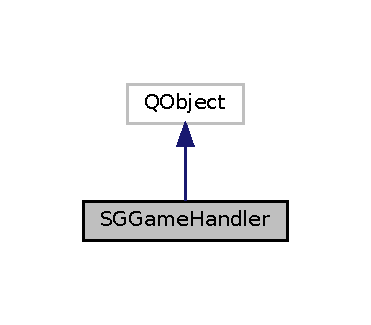
\includegraphics[width=178pt]{classSGGameHandler__inherit__graph}
\end{center}
\end{figure}


Collaboration diagram for S\+G\+Game\+Handler\+:
\nopagebreak
\begin{figure}[H]
\begin{center}
\leavevmode
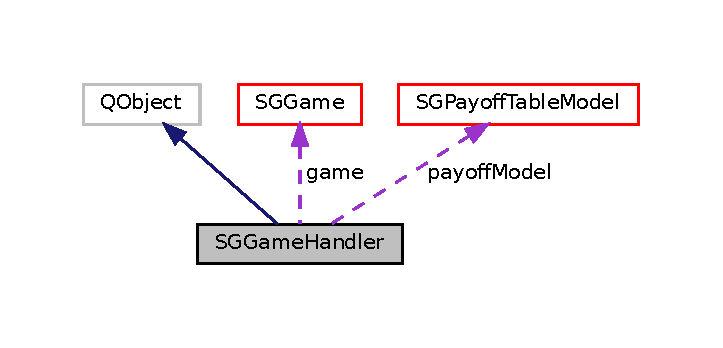
\includegraphics[width=347pt]{classSGGameHandler__coll__graph}
\end{center}
\end{figure}
\subsection*{Public Slots}
\begin{DoxyCompactItemize}
\item 
\mbox{\Hypertarget{classSGGameHandler_a1497e55ccf5e4a21f22f0326b5ccc2cc}\label{classSGGameHandler_a1497e55ccf5e4a21f22f0326b5ccc2cc}} 
void \hyperlink{classSGGameHandler_a1497e55ccf5e4a21f22f0326b5ccc2cc}{set\+Constrained} (int new\+State)
\begin{DoxyCompactList}\small\item\em Changes whether or not feasible set will be calculated. \end{DoxyCompactList}\end{DoxyCompactItemize}
\subsection*{Public Member Functions}
\begin{DoxyCompactItemize}
\item 
\hyperlink{classSGGameHandler_a2fe607ec68529ca4200cacf2e29725f9}{S\+G\+Game\+Handler} ()
\begin{DoxyCompactList}\small\item\em Constructor. \end{DoxyCompactList}\item 
\hyperlink{classSGGameHandler_a98ffa14cea717acb76411e0caceddbf7}{$\sim$\+S\+G\+Game\+Handler} ()
\begin{DoxyCompactList}\small\item\em Destructor. \end{DoxyCompactList}\item 
void \hyperlink{classSGGameHandler_a8ba6ee3d6e6648e1db7fe15d287b0277}{set\+Game} (const \hyperlink{classSGGame}{S\+G\+Game} \&\+\_\+game)
\begin{DoxyCompactList}\small\item\em Replaces the current game with \+\_\+game. \end{DoxyCompactList}\item 
\mbox{\Hypertarget{classSGGameHandler_a025753e9a17a82897ecca05fc59950ca}\label{classSGGameHandler_a025753e9a17a82897ecca05fc59950ca}} 
const \hyperlink{classSGGame}{S\+G\+Game} \& \hyperlink{classSGGameHandler_a025753e9a17a82897ecca05fc59950ca}{get\+Game} () const
\begin{DoxyCompactList}\small\item\em Returns constant reference to the current game. \end{DoxyCompactList}\item 
\mbox{\Hypertarget{classSGGameHandler_aeaf20cbbc2d1e2b6b3a6347f72fdfdfd}\label{classSGGameHandler_aeaf20cbbc2d1e2b6b3a6347f72fdfdfd}} 
double \hyperlink{classSGGameHandler_aeaf20cbbc2d1e2b6b3a6347f72fdfdfd}{get\+Error\+Tol} () const
\begin{DoxyCompactList}\small\item\em Returns the error tolerance. \end{DoxyCompactList}\item 
\mbox{\Hypertarget{classSGGameHandler_a23d30f5539cd59117864d767a57db11e}\label{classSGGameHandler_a23d30f5539cd59117864d767a57db11e}} 
Q\+V\+Box\+Layout $\ast$ \hyperlink{classSGGameHandler_a23d30f5539cd59117864d767a57db11e}{get\+Layout} () const
\begin{DoxyCompactList}\small\item\em Returns the layout. \end{DoxyCompactList}\item 
\mbox{\Hypertarget{classSGGameHandler_a8300ed57be8ed34010ef1f7cf0557067}\label{classSGGameHandler_a8300ed57be8ed34010ef1f7cf0557067}} 
Q\+Push\+Button $\ast$ \hyperlink{classSGGameHandler_a8300ed57be8ed34010ef1f7cf0557067}{get\+Solve\+Button} () const
\begin{DoxyCompactList}\small\item\em Returns the solve\+Button. \end{DoxyCompactList}\item 
\mbox{\Hypertarget{classSGGameHandler_af5af785b3b10ad782708fe8cfe93e371}\label{classSGGameHandler_af5af785b3b10ad782708fe8cfe93e371}} 
Q\+Push\+Button $\ast$ \hyperlink{classSGGameHandler_af5af785b3b10ad782708fe8cfe93e371}{get\+Solve\+Button\+\_\+\+V2} () const
\begin{DoxyCompactList}\small\item\em Returns the solve\+Button\+\_\+\+V2. \end{DoxyCompactList}\item 
\mbox{\Hypertarget{classSGGameHandler_a960e25dee1b13f27d4eb903f392e61e5}\label{classSGGameHandler_a960e25dee1b13f27d4eb903f392e61e5}} 
Q\+Push\+Button $\ast$ \hyperlink{classSGGameHandler_a960e25dee1b13f27d4eb903f392e61e5}{get\+Cancel\+Button} () const
\begin{DoxyCompactList}\small\item\em Returns the cancel\+Button. \end{DoxyCompactList}\item 
void \hyperlink{classSGGameHandler_a70b3147a78c94d3b7884b096a3a3a352}{set\+State} (int state)
\begin{DoxyCompactList}\small\item\em Changes the current state. \end{DoxyCompactList}\end{DoxyCompactItemize}
\subsection*{Private Slots}
\begin{DoxyCompactItemize}
\item 
\mbox{\Hypertarget{classSGGameHandler_a806f46e7a60e2c17530e6786245f7455}\label{classSGGameHandler_a806f46e7a60e2c17530e6786245f7455}} 
void \hyperlink{classSGGameHandler_a806f46e7a60e2c17530e6786245f7455}{current\+State\+Changed} (int newS)
\begin{DoxyCompactList}\small\item\em Slot for changing the state. Calls set\+State. \end{DoxyCompactList}\item 
\mbox{\Hypertarget{classSGGameHandler_a5e8650d00efcc8d41bfb04abb7edeb7b}\label{classSGGameHandler_a5e8650d00efcc8d41bfb04abb7edeb7b}} 
void \hyperlink{classSGGameHandler_a5e8650d00efcc8d41bfb04abb7edeb7b}{state\+Added} ()
\begin{DoxyCompactList}\small\item\em Adds a new state. Calls change\+Number\+Of\+States. \end{DoxyCompactList}\item 
\mbox{\Hypertarget{classSGGameHandler_aaf22c32b0431b81c05646e8acb2f6511}\label{classSGGameHandler_aaf22c32b0431b81c05646e8acb2f6511}} 
void \hyperlink{classSGGameHandler_aaf22c32b0431b81c05646e8acb2f6511}{action1\+Added} ()
\begin{DoxyCompactList}\small\item\em Action added for player 1. Calls action\+Added. \end{DoxyCompactList}\item 
\mbox{\Hypertarget{classSGGameHandler_abeb7b79db6493e8c2fdddb1e83b4dc01}\label{classSGGameHandler_abeb7b79db6493e8c2fdddb1e83b4dc01}} 
void \hyperlink{classSGGameHandler_abeb7b79db6493e8c2fdddb1e83b4dc01}{action2\+Added} ()
\begin{DoxyCompactList}\small\item\em Action added for player 2. Calls action\+Added. \end{DoxyCompactList}\item 
\mbox{\Hypertarget{classSGGameHandler_a6ead4477a6bc36eb73f220159ea2fa91}\label{classSGGameHandler_a6ead4477a6bc36eb73f220159ea2fa91}} 
void \hyperlink{classSGGameHandler_a6ead4477a6bc36eb73f220159ea2fa91}{action\+Added} (int player)
\begin{DoxyCompactList}\small\item\em Adds a new action for the indicated player. \end{DoxyCompactList}\item 
\mbox{\Hypertarget{classSGGameHandler_afd1cf958d916d9b1ee4a5aac70bc13ca}\label{classSGGameHandler_afd1cf958d916d9b1ee4a5aac70bc13ca}} 
void \hyperlink{classSGGameHandler_afd1cf958d916d9b1ee4a5aac70bc13ca}{state\+Removed} ()
\begin{DoxyCompactList}\small\item\em Removes the current state. \end{DoxyCompactList}\item 
\mbox{\Hypertarget{classSGGameHandler_ab3d00af463f833fd6417a754073494cc}\label{classSGGameHandler_ab3d00af463f833fd6417a754073494cc}} 
void \hyperlink{classSGGameHandler_ab3d00af463f833fd6417a754073494cc}{action1\+Removed} ()
\begin{DoxyCompactList}\small\item\em Action removed for player 1. Calls action\+Removed. \end{DoxyCompactList}\item 
\mbox{\Hypertarget{classSGGameHandler_ac55ea0d4296a14684c2735dd1c69c22e}\label{classSGGameHandler_ac55ea0d4296a14684c2735dd1c69c22e}} 
void \hyperlink{classSGGameHandler_ac55ea0d4296a14684c2735dd1c69c22e}{action2\+Removed} ()
\begin{DoxyCompactList}\small\item\em Action removed for player 2. Calls action\+Removed. \end{DoxyCompactList}\item 
void \hyperlink{classSGGameHandler_aed866fdb5315e2a593f659206eabbef3}{action\+Removed} (int player)
\begin{DoxyCompactList}\small\item\em Removes action for the given player. \end{DoxyCompactList}\item 
\mbox{\Hypertarget{classSGGameHandler_abfc41eef3937a69a3fa9d355f8f8afbb}\label{classSGGameHandler_abfc41eef3937a69a3fa9d355f8f8afbb}} 
void \hyperlink{classSGGameHandler_abfc41eef3937a69a3fa9d355f8f8afbb}{discount\+Factor\+Changed} (const Q\+String \&text)
\begin{DoxyCompactList}\small\item\em Changes the discount factor. \end{DoxyCompactList}\item 
\mbox{\Hypertarget{classSGGameHandler_aa556fc6fe75492c7e3eac05ccd54fe29}\label{classSGGameHandler_aa556fc6fe75492c7e3eac05ccd54fe29}} 
void \hyperlink{classSGGameHandler_aa556fc6fe75492c7e3eac05ccd54fe29}{error\+Tol\+Changed} (const Q\+String \&text)
\begin{DoxyCompactList}\small\item\em Changes the error tolerance. \end{DoxyCompactList}\item 
\mbox{\Hypertarget{classSGGameHandler_a0dcae7330df350da70211c7db489234b}\label{classSGGameHandler_a0dcae7330df350da70211c7db489234b}} 
void \hyperlink{classSGGameHandler_a0dcae7330df350da70211c7db489234b}{next\+State} ()
\begin{DoxyCompactList}\small\item\em Advances current\+State to the next state. \end{DoxyCompactList}\item 
\mbox{\Hypertarget{classSGGameHandler_a24a4f716b7b80be52d7092575d92767e}\label{classSGGameHandler_a24a4f716b7b80be52d7092575d92767e}} 
void \hyperlink{classSGGameHandler_a24a4f716b7b80be52d7092575d92767e}{prev\+State} ()
\begin{DoxyCompactList}\small\item\em Decreases current\+State to the previous state. \end{DoxyCompactList}\end{DoxyCompactItemize}
\subsection*{Private Member Functions}
\begin{DoxyCompactItemize}
\item 
void \hyperlink{classSGGameHandler_af80ac7a33ba124153e2be5528dbce4b7}{initialize\+Models} ()
\begin{DoxyCompactList}\small\item\em Delete old data models and create new ones. \end{DoxyCompactList}\item 
\mbox{\Hypertarget{classSGGameHandler_aef123beababcf909074f05772fbe88da}\label{classSGGameHandler_aef123beababcf909074f05772fbe88da}} 
void \hyperlink{classSGGameHandler_aef123beababcf909074f05772fbe88da}{push\+Back\+Probability\+Table} (int newS)
\begin{DoxyCompactList}\small\item\em Adds a new probability table model. \end{DoxyCompactList}\item 
\mbox{\Hypertarget{classSGGameHandler_a1b0499f2c29bc69ee73b0b7fa0678858}\label{classSGGameHandler_a1b0499f2c29bc69ee73b0b7fa0678858}} 
void \hyperlink{classSGGameHandler_a1b0499f2c29bc69ee73b0b7fa0678858}{pop\+Back\+Probability\+Table} ()
\begin{DoxyCompactList}\small\item\em Removes last probability table model. \end{DoxyCompactList}\item 
\mbox{\Hypertarget{classSGGameHandler_a7ea037a5ccc43686fad7f64944e65f82}\label{classSGGameHandler_a7ea037a5ccc43686fad7f64944e65f82}} 
void \hyperlink{classSGGameHandler_a7ea037a5ccc43686fad7f64944e65f82}{change\+Number\+Of\+States} (int newS)
\begin{DoxyCompactList}\small\item\em Adds/removes models to achieve correct number of states. \end{DoxyCompactList}\end{DoxyCompactItemize}
\subsection*{Private Attributes}
\begin{DoxyCompactItemize}
\item 
\hyperlink{classSGGame}{S\+G\+Game} \hyperlink{classSGGameHandler_ac95a8d363c98979cbbd8fc63a112bf11}{game}
\begin{DoxyCompactList}\small\item\em The game object. \end{DoxyCompactList}\item 
\mbox{\Hypertarget{classSGGameHandler_a43b882271dcb9673494a960d469cd2df}\label{classSGGameHandler_a43b882271dcb9673494a960d469cd2df}} 
double \hyperlink{classSGGameHandler_a43b882271dcb9673494a960d469cd2df}{error\+Tol}
\begin{DoxyCompactList}\small\item\em Error tolerance for measuring convergence. \end{DoxyCompactList}\item 
\mbox{\Hypertarget{classSGGameHandler_a515fcf42da91b1181f9663c280caf48b}\label{classSGGameHandler_a515fcf42da91b1181f9663c280caf48b}} 
\hyperlink{classSGPayoffTableModel}{S\+G\+Payoff\+Table\+Model} $\ast$ \hyperlink{classSGGameHandler_a515fcf42da91b1181f9663c280caf48b}{payoff\+Model}
\begin{DoxyCompactList}\small\item\em The model for interfacing with payoffs. \end{DoxyCompactList}\item 
\mbox{\Hypertarget{classSGGameHandler_a4f7c265204b97594fe70e98ddc4fb559}\label{classSGGameHandler_a4f7c265204b97594fe70e98ddc4fb559}} 
vector$<$ \hyperlink{classSGProbabilityTableModel}{S\+G\+Probability\+Table\+Model} $\ast$ $>$ \hyperlink{classSGGameHandler_a4f7c265204b97594fe70e98ddc4fb559}{probability\+Models}
\begin{DoxyCompactList}\small\item\em Vector of models for interfacing with transition probabilities. \end{DoxyCompactList}\item 
\mbox{\Hypertarget{classSGGameHandler_a2cf4dd4571399321e16d89d882d08715}\label{classSGGameHandler_a2cf4dd4571399321e16d89d882d08715}} 
Q\+V\+Box\+Layout $\ast$ \hyperlink{classSGGameHandler_a2cf4dd4571399321e16d89d882d08715}{layout}
\begin{DoxyCompactList}\small\item\em Layout for the game tab. \end{DoxyCompactList}\item 
\mbox{\Hypertarget{classSGGameHandler_a2ea8dd4650b9ac752f26b575577def3b}\label{classSGGameHandler_a2ea8dd4650b9ac752f26b575577def3b}} 
Q\+Push\+Button $\ast$ \hyperlink{classSGGameHandler_a2ea8dd4650b9ac752f26b575577def3b}{solve\+Button}
\begin{DoxyCompactList}\small\item\em Button that triggers solve routine. \end{DoxyCompactList}\item 
\mbox{\Hypertarget{classSGGameHandler_afbb441f7d9e95ce509c0fc8198aac65b}\label{classSGGameHandler_afbb441f7d9e95ce509c0fc8198aac65b}} 
Q\+Push\+Button $\ast$ \hyperlink{classSGGameHandler_afbb441f7d9e95ce509c0fc8198aac65b}{solve\+Button\+\_\+\+V2}
\begin{DoxyCompactList}\small\item\em Button that triggers solve routine. \end{DoxyCompactList}\item 
\mbox{\Hypertarget{classSGGameHandler_a667ac1db8acfa5b7aca6ace606e17e80}\label{classSGGameHandler_a667ac1db8acfa5b7aca6ace606e17e80}} 
Q\+Push\+Button $\ast$ \hyperlink{classSGGameHandler_a667ac1db8acfa5b7aca6ace606e17e80}{cancel\+Button}
\begin{DoxyCompactList}\small\item\em Button that cancels solve. \end{DoxyCompactList}\item 
\mbox{\Hypertarget{classSGGameHandler_a4ac6ec9392bf0dbf0c1d7b5e9643e2a9}\label{classSGGameHandler_a4ac6ec9392bf0dbf0c1d7b5e9643e2a9}} 
Q\+Line\+Edit $\ast$ \hyperlink{classSGGameHandler_a4ac6ec9392bf0dbf0c1d7b5e9643e2a9}{delta\+Edit}
\begin{DoxyCompactList}\small\item\em For editing the discount factor. \end{DoxyCompactList}\item 
\mbox{\Hypertarget{classSGGameHandler_af781ae067fa7402743f2f494ab4ff20f}\label{classSGGameHandler_af781ae067fa7402743f2f494ab4ff20f}} 
vector$<$ Q\+Line\+Edit $\ast$ $>$ \hyperlink{classSGGameHandler_af781ae067fa7402743f2f494ab4ff20f}{num\+Actions\+Edits}
\begin{DoxyCompactList}\small\item\em Vector of edits for players\textquotesingle{} numbers of actions. \end{DoxyCompactList}\item 
\mbox{\Hypertarget{classSGGameHandler_afb806d54a9d193c5ab8e3a1510001fba}\label{classSGGameHandler_afb806d54a9d193c5ab8e3a1510001fba}} 
Q\+Line\+Edit $\ast$ \hyperlink{classSGGameHandler_afb806d54a9d193c5ab8e3a1510001fba}{num\+States\+Edit}
\begin{DoxyCompactList}\small\item\em Edit for number of states. \end{DoxyCompactList}\item 
\mbox{\Hypertarget{classSGGameHandler_aec404b883f476d06e7d19dd3a1ea7336}\label{classSGGameHandler_aec404b883f476d06e7d19dd3a1ea7336}} 
Q\+Line\+Edit $\ast$ \hyperlink{classSGGameHandler_aec404b883f476d06e7d19dd3a1ea7336}{error\+Tol\+Edit}
\begin{DoxyCompactList}\small\item\em Edit for controlling error tolerance. \end{DoxyCompactList}\item 
\mbox{\Hypertarget{classSGGameHandler_af722a69ea2f4a6a5c56171a2126aac5c}\label{classSGGameHandler_af722a69ea2f4a6a5c56171a2126aac5c}} 
Q\+Combo\+Box $\ast$ \hyperlink{classSGGameHandler_af722a69ea2f4a6a5c56171a2126aac5c}{current\+State\+Combo}
\begin{DoxyCompactList}\small\item\em Drop down menu for selecting a state. \end{DoxyCompactList}\item 
\mbox{\Hypertarget{classSGGameHandler_a5c40be01364eb863bc087776648be235}\label{classSGGameHandler_a5c40be01364eb863bc087776648be235}} 
Q\+Table\+View $\ast$ \hyperlink{classSGGameHandler_a5c40be01364eb863bc087776648be235}{payoff\+Table\+View}
\begin{DoxyCompactList}\small\item\em Table for displaying stage payoffs. \end{DoxyCompactList}\item 
\mbox{\Hypertarget{classSGGameHandler_a2e6f4e94869b83d54badeb5c5f1f8e64}\label{classSGGameHandler_a2e6f4e94869b83d54badeb5c5f1f8e64}} 
vector$<$ \hyperlink{classSGTableView}{S\+G\+Table\+View} $\ast$ $>$ \hyperlink{classSGGameHandler_a2e6f4e94869b83d54badeb5c5f1f8e64}{probability\+Table\+Views}
\begin{DoxyCompactList}\small\item\em Vector of tables for displaying transition probabilities. \end{DoxyCompactList}\item 
\mbox{\Hypertarget{classSGGameHandler_a4c3c643906ccdf6283666007c4f8a49e}\label{classSGGameHandler_a4c3c643906ccdf6283666007c4f8a49e}} 
Q\+V\+Box\+Layout $\ast$ \hyperlink{classSGGameHandler_a4c3c643906ccdf6283666007c4f8a49e}{probability\+Table\+Layout}
\begin{DoxyCompactList}\small\item\em Layout for holding transition probability tables. \end{DoxyCompactList}\item 
\mbox{\Hypertarget{classSGGameHandler_a6ec21010dfb89d193762bf8c8d443394}\label{classSGGameHandler_a6ec21010dfb89d193762bf8c8d443394}} 
Q\+Check\+Box $\ast$ \hyperlink{classSGGameHandler_a6ec21010dfb89d193762bf8c8d443394}{feasible\+Check\+Box}
\begin{DoxyCompactList}\small\item\em Check box for whether or not to calculate feasible set. \end{DoxyCompactList}\end{DoxyCompactItemize}


\subsection{Detailed Description}
This class handles the widgets for editing/displaying the game. 

All of the widgets in the game tab and their slots are members of this class. It also contains the pointer to the \hyperlink{classSGGame}{S\+G\+Game}, and handles the interfaces to the game objects.

The class contains table models for editing the game, which interface with the respective data using the \hyperlink{classSGGame}{S\+G\+Game} class\textquotesingle{}s interface methods.

For a more detailed description, see viewergametabsec. 

\subsection{Constructor \& Destructor Documentation}
\mbox{\Hypertarget{classSGGameHandler_a2fe607ec68529ca4200cacf2e29725f9}\label{classSGGameHandler_a2fe607ec68529ca4200cacf2e29725f9}} 
\index{S\+G\+Game\+Handler@{S\+G\+Game\+Handler}!S\+G\+Game\+Handler@{S\+G\+Game\+Handler}}
\index{S\+G\+Game\+Handler@{S\+G\+Game\+Handler}!S\+G\+Game\+Handler@{S\+G\+Game\+Handler}}
\subsubsection{\texorpdfstring{S\+G\+Game\+Handler()}{SGGameHandler()}}
{\footnotesize\ttfamily S\+G\+Game\+Handler\+::\+S\+G\+Game\+Handler (\begin{DoxyParamCaption}{ }\end{DoxyParamCaption})}



Constructor. 

Constructs edits and buttons, connects signals/slots, calls \hyperlink{classSGGameHandler_af80ac7a33ba124153e2be5528dbce4b7}{S\+G\+Game\+Handler\+::initialize\+Models}. \mbox{\Hypertarget{classSGGameHandler_a98ffa14cea717acb76411e0caceddbf7}\label{classSGGameHandler_a98ffa14cea717acb76411e0caceddbf7}} 
\index{S\+G\+Game\+Handler@{S\+G\+Game\+Handler}!````~S\+G\+Game\+Handler@{$\sim$\+S\+G\+Game\+Handler}}
\index{````~S\+G\+Game\+Handler@{$\sim$\+S\+G\+Game\+Handler}!S\+G\+Game\+Handler@{S\+G\+Game\+Handler}}
\subsubsection{\texorpdfstring{$\sim$\+S\+G\+Game\+Handler()}{~SGGameHandler()}}
{\footnotesize\ttfamily S\+G\+Game\+Handler\+::$\sim$\+S\+G\+Game\+Handler (\begin{DoxyParamCaption}{ }\end{DoxyParamCaption})}



Destructor. 

Destroys probability table views, models, etc. 

\subsection{Member Function Documentation}
\mbox{\Hypertarget{classSGGameHandler_aed866fdb5315e2a593f659206eabbef3}\label{classSGGameHandler_aed866fdb5315e2a593f659206eabbef3}} 
\index{S\+G\+Game\+Handler@{S\+G\+Game\+Handler}!action\+Removed@{action\+Removed}}
\index{action\+Removed@{action\+Removed}!S\+G\+Game\+Handler@{S\+G\+Game\+Handler}}
\subsubsection{\texorpdfstring{action\+Removed}{actionRemoved}}
{\footnotesize\ttfamily void S\+G\+Game\+Handler\+::action\+Removed (\begin{DoxyParamCaption}\item[{int}]{player }\end{DoxyParamCaption})\hspace{0.3cm}{\ttfamily [private]}, {\ttfamily [slot]}}



Removes action for the given player. 

Will remove the action that is currently selected in the payoff table, if one is selected. \mbox{\Hypertarget{classSGGameHandler_af80ac7a33ba124153e2be5528dbce4b7}\label{classSGGameHandler_af80ac7a33ba124153e2be5528dbce4b7}} 
\index{S\+G\+Game\+Handler@{S\+G\+Game\+Handler}!initialize\+Models@{initialize\+Models}}
\index{initialize\+Models@{initialize\+Models}!S\+G\+Game\+Handler@{S\+G\+Game\+Handler}}
\subsubsection{\texorpdfstring{initialize\+Models()}{initializeModels()}}
{\footnotesize\ttfamily void S\+G\+Game\+Handler\+::initialize\+Models (\begin{DoxyParamCaption}{ }\end{DoxyParamCaption})\hspace{0.3cm}{\ttfamily [private]}}



Delete old data models and create new ones. 

Called in constructor and whenever game changes. \mbox{\Hypertarget{classSGGameHandler_a8ba6ee3d6e6648e1db7fe15d287b0277}\label{classSGGameHandler_a8ba6ee3d6e6648e1db7fe15d287b0277}} 
\index{S\+G\+Game\+Handler@{S\+G\+Game\+Handler}!set\+Game@{set\+Game}}
\index{set\+Game@{set\+Game}!S\+G\+Game\+Handler@{S\+G\+Game\+Handler}}
\subsubsection{\texorpdfstring{set\+Game()}{setGame()}}
{\footnotesize\ttfamily void S\+G\+Game\+Handler\+::set\+Game (\begin{DoxyParamCaption}\item[{const \hyperlink{classSGGame}{S\+G\+Game} \&}]{\+\_\+game }\end{DoxyParamCaption})}



Replaces the current game with \+\_\+game. 

Calls initialize\+Models to reinitialize references for table models. \mbox{\Hypertarget{classSGGameHandler_a70b3147a78c94d3b7884b096a3a3a352}\label{classSGGameHandler_a70b3147a78c94d3b7884b096a3a3a352}} 
\index{S\+G\+Game\+Handler@{S\+G\+Game\+Handler}!set\+State@{set\+State}}
\index{set\+State@{set\+State}!S\+G\+Game\+Handler@{S\+G\+Game\+Handler}}
\subsubsection{\texorpdfstring{set\+State()}{setState()}}
{\footnotesize\ttfamily void S\+G\+Game\+Handler\+::set\+State (\begin{DoxyParamCaption}\item[{int}]{state }\end{DoxyParamCaption})}



Changes the current state. 

Switches all of the models over to new state and updates table views. 

\subsection{Member Data Documentation}
\mbox{\Hypertarget{classSGGameHandler_ac95a8d363c98979cbbd8fc63a112bf11}\label{classSGGameHandler_ac95a8d363c98979cbbd8fc63a112bf11}} 
\index{S\+G\+Game\+Handler@{S\+G\+Game\+Handler}!game@{game}}
\index{game@{game}!S\+G\+Game\+Handler@{S\+G\+Game\+Handler}}
\subsubsection{\texorpdfstring{game}{game}}
{\footnotesize\ttfamily \hyperlink{classSGGame}{S\+G\+Game} S\+G\+Game\+Handler\+::game\hspace{0.3cm}{\ttfamily [private]}}



The game object. 

This is the game that is represented in the game tab. Note that this can be a different game than the one that is associated with the solution in the solution tab. 

The documentation for this class was generated from the following files\+:\begin{DoxyCompactItemize}
\item 
viewer/hpp/sggamehandler.\+hpp\item 
viewer/cpp/sggamehandler.\+cpp\end{DoxyCompactItemize}

\hypertarget{classSGHyperplane}{}\section{S\+G\+Hyperplane Class Reference}
\label{classSGHyperplane}\index{S\+G\+Hyperplane@{S\+G\+Hyperplane}}


Represents a hyperplane in $\mathbb{R}^N$.  




{\ttfamily \#include $<$sghyperplane.\+hpp$>$}



Collaboration diagram for S\+G\+Hyperplane\+:
\nopagebreak
\begin{figure}[H]
\begin{center}
\leavevmode
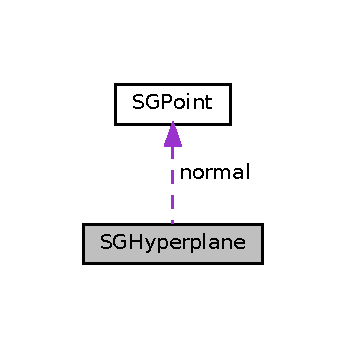
\includegraphics[width=166pt]{classSGHyperplane__coll__graph}
\end{center}
\end{figure}
\subsection*{Public Member Functions}
\begin{DoxyCompactItemize}
\item 
\mbox{\Hypertarget{classSGHyperplane_a4fd24c9b78e60211ffe894949ae8b5d0}\label{classSGHyperplane_a4fd24c9b78e60211ffe894949ae8b5d0}} 
\hyperlink{classSGHyperplane_a4fd24c9b78e60211ffe894949ae8b5d0}{S\+G\+Hyperplane} (int num\+States)
\begin{DoxyCompactList}\small\item\em Initializes tuple to \+\_\+num\+States zero-\/vectors. \end{DoxyCompactList}\item 
\mbox{\Hypertarget{classSGHyperplane_a002bf1b44c69989e472582d669cf4342}\label{classSGHyperplane_a002bf1b44c69989e472582d669cf4342}} 
\hyperlink{classSGHyperplane_a002bf1b44c69989e472582d669cf4342}{S\+G\+Hyperplane} (const \hyperlink{classSGPoint}{S\+G\+Point} \&\+\_\+normal, const vector$<$ double $>$ \&\+\_\+levels)
\begin{DoxyCompactList}\small\item\em Initializes tuple to \+\_\+num\+Points copies of point. \end{DoxyCompactList}\item 
\mbox{\Hypertarget{classSGHyperplane_a2154f1656b3b98398be07aae43294c5d}\label{classSGHyperplane_a2154f1656b3b98398be07aae43294c5d}} 
\hyperlink{classSGHyperplane_a2154f1656b3b98398be07aae43294c5d}{S\+G\+Hyperplane} ()
\begin{DoxyCompactList}\small\item\em Default constructor for empty tuple. \end{DoxyCompactList}\item 
double \hyperlink{classSGHyperplane_a54ab1a4f18536c7eef048fb6579e797a}{expectation} (const vector$<$ double $>$ \&prob) const
\begin{DoxyCompactList}\small\item\em Mathematical expectation. \end{DoxyCompactList}\item 
\mbox{\Hypertarget{classSGHyperplane_a62b2eccbe7ef8c8623416e3d992e1f91}\label{classSGHyperplane_a62b2eccbe7ef8c8623416e3d992e1f91}} 
void \hyperlink{classSGHyperplane_a62b2eccbe7ef8c8623416e3d992e1f91}{push\+\_\+back} (double level)
\begin{DoxyCompactList}\small\item\em Adds a new level to the back of the hyperplane. \end{DoxyCompactList}\item 
\mbox{\Hypertarget{classSGHyperplane_a38e2a9c26b1c58f8e0c585614f318628}\label{classSGHyperplane_a38e2a9c26b1c58f8e0c585614f318628}} 
void \hyperlink{classSGHyperplane_a38e2a9c26b1c58f8e0c585614f318628}{clear} ()
\begin{DoxyCompactList}\small\item\em Sets the levels equal to an empty vector. \end{DoxyCompactList}\item 
\mbox{\Hypertarget{classSGHyperplane_ab3e09fc609822cf940419acff48b0493}\label{classSGHyperplane_ab3e09fc609822cf940419acff48b0493}} 
int \hyperlink{classSGHyperplane_ab3e09fc609822cf940419acff48b0493}{size} () const
\begin{DoxyCompactList}\small\item\em Returns the number of levels in the tuple. \end{DoxyCompactList}\item 
\mbox{\Hypertarget{classSGHyperplane_af6425968a114ae5b9f3716220a6a9f31}\label{classSGHyperplane_af6425968a114ae5b9f3716220a6a9f31}} 
void \hyperlink{classSGHyperplane_af6425968a114ae5b9f3716220a6a9f31}{set\+Normal} (const \hyperlink{classSGPoint}{S\+G\+Point} \&new\+Norm)
\begin{DoxyCompactList}\small\item\em Set the normal. \end{DoxyCompactList}\item 
\mbox{\Hypertarget{classSGHyperplane_a380197ed5db29754ee75c7628aef53e5}\label{classSGHyperplane_a380197ed5db29754ee75c7628aef53e5}} 
const \hyperlink{classSGPoint}{S\+G\+Point} \& \hyperlink{classSGHyperplane_a380197ed5db29754ee75c7628aef53e5}{get\+Normal} () const
\begin{DoxyCompactList}\small\item\em Get the normal. \end{DoxyCompactList}\item 
\mbox{\Hypertarget{classSGHyperplane_af7232a6b42e6aec55e4a1cf93d9c9fd3}\label{classSGHyperplane_af7232a6b42e6aec55e4a1cf93d9c9fd3}} 
const vector$<$ double $>$ \& \hyperlink{classSGHyperplane_af7232a6b42e6aec55e4a1cf93d9c9fd3}{get\+Levels} () const
\begin{DoxyCompactList}\small\item\em Get the levels. \end{DoxyCompactList}\item 
\mbox{\Hypertarget{classSGHyperplane_a4a074f4db5c1b9440adfc6a26ef849ec}\label{classSGHyperplane_a4a074f4db5c1b9440adfc6a26ef849ec}} 
double \& \hyperlink{classSGHyperplane_a4a074f4db5c1b9440adfc6a26ef849ec}{operator\mbox{[}$\,$\mbox{]}} (int state)
\begin{DoxyCompactList}\small\item\em Random access the elements of the tuple. \end{DoxyCompactList}\item 
\mbox{\Hypertarget{classSGHyperplane_a12547087ec56fa4148d6057ab9bf04b2}\label{classSGHyperplane_a12547087ec56fa4148d6057ab9bf04b2}} 
const double \& \hyperlink{classSGHyperplane_a12547087ec56fa4148d6057ab9bf04b2}{operator\mbox{[}$\,$\mbox{]}} (int state) const
\begin{DoxyCompactList}\small\item\em Constant random access to elements of the tuple. \end{DoxyCompactList}\item 
\mbox{\Hypertarget{classSGHyperplane_ab4450942532a7322912aac2f4369f6f2}\label{classSGHyperplane_ab4450942532a7322912aac2f4369f6f2}} 
\hyperlink{classSGHyperplane}{S\+G\+Hyperplane} \& \hyperlink{classSGHyperplane_ab4450942532a7322912aac2f4369f6f2}{operator=} (const \hyperlink{classSGHyperplane}{S\+G\+Hyperplane} \&rhs)
\begin{DoxyCompactList}\small\item\em Assignment operator. \end{DoxyCompactList}\item 
\mbox{\Hypertarget{classSGHyperplane_af3570931974fe91ac522711273ac8c77}\label{classSGHyperplane_af3570931974fe91ac522711273ac8c77}} 
\hyperlink{classSGHyperplane}{S\+G\+Hyperplane} \& \hyperlink{classSGHyperplane_af3570931974fe91ac522711273ac8c77}{operator+=} (const \hyperlink{classSGHyperplane}{S\+G\+Hyperplane} \&rhs)
\begin{DoxyCompactList}\small\item\em Augmented addition of tuples. \end{DoxyCompactList}\item 
\mbox{\Hypertarget{classSGHyperplane_a533fe06af60ebb131b188706aa8b7dcc}\label{classSGHyperplane_a533fe06af60ebb131b188706aa8b7dcc}} 
\hyperlink{classSGHyperplane}{S\+G\+Hyperplane} \& \hyperlink{classSGHyperplane_a533fe06af60ebb131b188706aa8b7dcc}{operator-\/=} (const \hyperlink{classSGHyperplane}{S\+G\+Hyperplane} \&rhs)
\begin{DoxyCompactList}\small\item\em Augmented subtraction of tuples. \end{DoxyCompactList}\item 
\hyperlink{classSGHyperplane}{S\+G\+Hyperplane} \& \hyperlink{classSGHyperplane_a8ae5f73b29eb37d186e28e2397d27eca}{operator+=} (double rhs)
\begin{DoxyCompactList}\small\item\em Augmented addition of tuple with a point. \end{DoxyCompactList}\item 
\mbox{\Hypertarget{classSGHyperplane_a8f06272872b7401c2b3fb813edf6598c}\label{classSGHyperplane_a8f06272872b7401c2b3fb813edf6598c}} 
\hyperlink{classSGHyperplane}{S\+G\+Hyperplane} \& \hyperlink{classSGHyperplane_a8f06272872b7401c2b3fb813edf6598c}{operator$\ast$=} (double d)
\begin{DoxyCompactList}\small\item\em Scalar multiplication of the hyperplane. \end{DoxyCompactList}\item 
\mbox{\Hypertarget{classSGHyperplane_a02ec6baabcf5857e6fd2499b587fe9fc}\label{classSGHyperplane_a02ec6baabcf5857e6fd2499b587fe9fc}} 
void \hyperlink{classSGHyperplane_a02ec6baabcf5857e6fd2499b587fe9fc}{round} (double tol)
\begin{DoxyCompactList}\small\item\em Round off significant digits smaller than tol. \end{DoxyCompactList}\item 
\mbox{\Hypertarget{classSGHyperplane_a667377972806a13c704dcd728340878d}\label{classSGHyperplane_a667377972806a13c704dcd728340878d}} 
{\footnotesize template$<$class Archive $>$ }\\void \hyperlink{classSGHyperplane_a667377972806a13c704dcd728340878d}{serialize} (Archive \&ar, const unsigned int version)
\begin{DoxyCompactList}\small\item\em Serialize using boost. \end{DoxyCompactList}\end{DoxyCompactItemize}
\subsection*{Static Public Member Functions}
\begin{DoxyCompactItemize}
\item 
\mbox{\Hypertarget{classSGHyperplane_abe0d95282d0fe15ea7ac5e1d138ea527}\label{classSGHyperplane_abe0d95282d0fe15ea7ac5e1d138ea527}} 
static double \hyperlink{classSGHyperplane_abe0d95282d0fe15ea7ac5e1d138ea527}{distance} (const \hyperlink{classSGHyperplane}{S\+G\+Hyperplane} \&t0, const \hyperlink{classSGHyperplane}{S\+G\+Hyperplane} \&t1)
\begin{DoxyCompactList}\small\item\em Calculates the distance between t0 and t1 in the sup norm. \end{DoxyCompactList}\end{DoxyCompactItemize}
\subsection*{Private Attributes}
\begin{DoxyCompactItemize}
\item 
\hyperlink{classSGPoint}{S\+G\+Point} \hyperlink{classSGHyperplane_ac5855eb45d21dc29a4770ad335a426e6}{normal}
\item 
vector$<$ double $>$ \hyperlink{classSGHyperplane_a0da64d24816c2d70c84aeaf405035416}{levels}
\end{DoxyCompactItemize}
\subsection*{Friends}
\begin{DoxyCompactItemize}
\item 
\mbox{\Hypertarget{classSGHyperplane_ac98d07dd8f7b70e16ccb9a01abf56b9c}\label{classSGHyperplane_ac98d07dd8f7b70e16ccb9a01abf56b9c}} 
class {\bfseries boost\+::serialization\+::access}
\item 
\mbox{\Hypertarget{classSGHyperplane_a93b21e7662e8dfa8780bf805ef59f8ba}\label{classSGHyperplane_a93b21e7662e8dfa8780bf805ef59f8ba}} 
\hyperlink{classSGHyperplane}{S\+G\+Hyperplane} \hyperlink{classSGHyperplane_a93b21e7662e8dfa8780bf805ef59f8ba}{operator$\ast$} (double d, const \hyperlink{classSGHyperplane}{S\+G\+Hyperplane} \&hp)
\begin{DoxyCompactList}\small\item\em Left scalar multiplication of a tuple. \end{DoxyCompactList}\item 
\mbox{\Hypertarget{classSGHyperplane_a7ee3d1e4a61b951d5687af84b06e49e4}\label{classSGHyperplane_a7ee3d1e4a61b951d5687af84b06e49e4}} 
\hyperlink{classSGHyperplane}{S\+G\+Hyperplane} \hyperlink{classSGHyperplane_a7ee3d1e4a61b951d5687af84b06e49e4}{operator$\ast$} (const \hyperlink{classSGHyperplane}{S\+G\+Hyperplane} \&hp, double d)
\begin{DoxyCompactList}\small\item\em Right scalar multiplication of a tuple. \end{DoxyCompactList}\item 
\mbox{\Hypertarget{classSGHyperplane_a2e0ac25ee46e85b3df26d063fccc23cf}\label{classSGHyperplane_a2e0ac25ee46e85b3df26d063fccc23cf}} 
ostream \& \hyperlink{classSGHyperplane_a2e0ac25ee46e85b3df26d063fccc23cf}{operator$<$$<$} (ostream \&out, const \hyperlink{classSGHyperplane}{S\+G\+Hyperplane} \&rhs)
\begin{DoxyCompactList}\small\item\em Output formatted tuple to file stream. \end{DoxyCompactList}\end{DoxyCompactItemize}


\subsection{Detailed Description}
Represents a hyperplane in $\mathbb{R}^N$. 

Consists of a normal direction and a vector of levels, one for each state.

Used to represent half spaces in \hyperlink{classSGSolver__MaxMinMax}{S\+G\+Solver\+\_\+\+Max\+Min\+Max} and \hyperlink{classSGSolver__MaxMinMax__3Player}{S\+G\+Solver\+\_\+\+Max\+Min\+Max\+\_\+3\+Player}. 

\subsection{Member Function Documentation}
\mbox{\Hypertarget{classSGHyperplane_a54ab1a4f18536c7eef048fb6579e797a}\label{classSGHyperplane_a54ab1a4f18536c7eef048fb6579e797a}} 
\index{S\+G\+Hyperplane@{S\+G\+Hyperplane}!expectation@{expectation}}
\index{expectation@{expectation}!S\+G\+Hyperplane@{S\+G\+Hyperplane}}
\subsubsection{\texorpdfstring{expectation()}{expectation()}}
{\footnotesize\ttfamily double S\+G\+Hyperplane\+::expectation (\begin{DoxyParamCaption}\item[{const vector$<$ double $>$ \&}]{prob }\end{DoxyParamCaption}) const}



Mathematical expectation. 

Returns the weighted sum of the levels using the weights in prob. \mbox{\Hypertarget{classSGHyperplane_a8ae5f73b29eb37d186e28e2397d27eca}\label{classSGHyperplane_a8ae5f73b29eb37d186e28e2397d27eca}} 
\index{S\+G\+Hyperplane@{S\+G\+Hyperplane}!operator+=@{operator+=}}
\index{operator+=@{operator+=}!S\+G\+Hyperplane@{S\+G\+Hyperplane}}
\subsubsection{\texorpdfstring{operator+=()}{operator+=()}}
{\footnotesize\ttfamily \hyperlink{classSGHyperplane}{S\+G\+Hyperplane}\& S\+G\+Hyperplane\+::operator+= (\begin{DoxyParamCaption}\item[{double}]{rhs }\end{DoxyParamCaption})}



Augmented addition of tuple with a point. 

Adds rhs to each level. 

\subsection{Member Data Documentation}
\mbox{\Hypertarget{classSGHyperplane_a0da64d24816c2d70c84aeaf405035416}\label{classSGHyperplane_a0da64d24816c2d70c84aeaf405035416}} 
\index{S\+G\+Hyperplane@{S\+G\+Hyperplane}!levels@{levels}}
\index{levels@{levels}!S\+G\+Hyperplane@{S\+G\+Hyperplane}}
\subsubsection{\texorpdfstring{levels}{levels}}
{\footnotesize\ttfamily vector$<$double$>$ S\+G\+Hyperplane\+::levels\hspace{0.3cm}{\ttfamily [private]}}

Level attained in each state. \mbox{\Hypertarget{classSGHyperplane_ac5855eb45d21dc29a4770ad335a426e6}\label{classSGHyperplane_ac5855eb45d21dc29a4770ad335a426e6}} 
\index{S\+G\+Hyperplane@{S\+G\+Hyperplane}!normal@{normal}}
\index{normal@{normal}!S\+G\+Hyperplane@{S\+G\+Hyperplane}}
\subsubsection{\texorpdfstring{normal}{normal}}
{\footnotesize\ttfamily \hyperlink{classSGPoint}{S\+G\+Point} S\+G\+Hyperplane\+::normal\hspace{0.3cm}{\ttfamily [private]}}

Normal normal to the hyperplanes. 

The documentation for this class was generated from the following files\+:\begin{DoxyCompactItemize}
\item 
src/hpp/sghyperplane.\+hpp\item 
src/cpp/sghyperplane.\+cpp\end{DoxyCompactItemize}

\hypertarget{classSGIntAttrEdit}{}\section{S\+G\+Int\+Attr\+Edit Class Reference}
\label{classSGIntAttrEdit}\index{S\+G\+Int\+Attr\+Edit@{S\+G\+Int\+Attr\+Edit}}


A widget for editing integer attributes.  




{\ttfamily \#include $<$sgrisksharinghandler.\+hpp$>$}



Inheritance diagram for S\+G\+Int\+Attr\+Edit\+:
\nopagebreak
\begin{figure}[H]
\begin{center}
\leavevmode
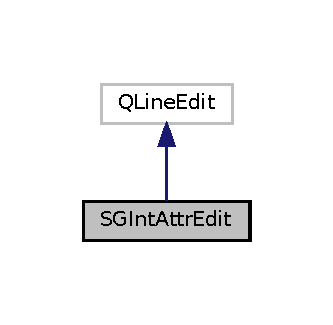
\includegraphics[width=160pt]{classSGIntAttrEdit__inherit__graph}
\end{center}
\end{figure}


Collaboration diagram for S\+G\+Int\+Attr\+Edit\+:
\nopagebreak
\begin{figure}[H]
\begin{center}
\leavevmode
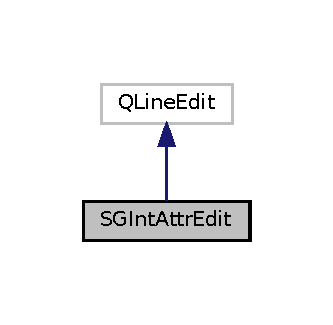
\includegraphics[width=160pt]{classSGIntAttrEdit__coll__graph}
\end{center}
\end{figure}
\subsection*{Public Member Functions}
\begin{DoxyCompactItemize}
\item 
\mbox{\Hypertarget{classSGIntAttrEdit_a83831c89273f82b5ab2d44fac2f3c970}\label{classSGIntAttrEdit_a83831c89273f82b5ab2d44fac2f3c970}} 
\hyperlink{classSGIntAttrEdit_a83831c89273f82b5ab2d44fac2f3c970}{S\+G\+Int\+Attr\+Edit} (int \&\+\_\+attr)
\begin{DoxyCompactList}\small\item\em Constructor. \end{DoxyCompactList}\end{DoxyCompactItemize}
\subsection*{Private Slots}
\begin{DoxyCompactItemize}
\item 
\mbox{\Hypertarget{classSGIntAttrEdit_a2a8918c9b08a451d63779566f102391b}\label{classSGIntAttrEdit_a2a8918c9b08a451d63779566f102391b}} 
void \hyperlink{classSGIntAttrEdit_a2a8918c9b08a451d63779566f102391b}{change\+Attr} (const Q\+String \&text)
\begin{DoxyCompactList}\small\item\em Slot called when Q\+Line\+Edit is edited. \end{DoxyCompactList}\end{DoxyCompactItemize}
\subsection*{Private Attributes}
\begin{DoxyCompactItemize}
\item 
\mbox{\Hypertarget{classSGIntAttrEdit_ac7a5de9b8735b5f0d1f39759c833fd4f}\label{classSGIntAttrEdit_ac7a5de9b8735b5f0d1f39759c833fd4f}} 
int \& \hyperlink{classSGIntAttrEdit_ac7a5de9b8735b5f0d1f39759c833fd4f}{attr}
\begin{DoxyCompactList}\small\item\em Reference to the attribute. \end{DoxyCompactList}\end{DoxyCompactItemize}


\subsection{Detailed Description}
A widget for editing integer attributes. 

The documentation for this class was generated from the following file\+:\begin{DoxyCompactItemize}
\item 
viewer/hpp/sgrisksharinghandler.\+hpp\end{DoxyCompactItemize}

\hypertarget{classSGIntParamEdit}{}\section{S\+G\+Int\+Param\+Edit Class Reference}
\label{classSGIntParamEdit}\index{S\+G\+Int\+Param\+Edit@{S\+G\+Int\+Param\+Edit}}


Class for changing integer parameters.  




{\ttfamily \#include $<$sgsettingshandler.\+hpp$>$}



Inheritance diagram for S\+G\+Int\+Param\+Edit\+:
\nopagebreak
\begin{figure}[H]
\begin{center}
\leavevmode
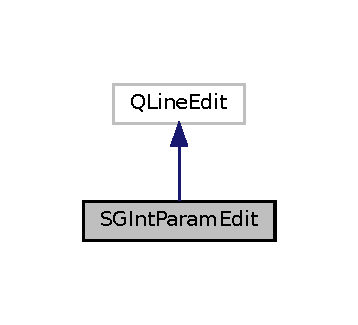
\includegraphics[width=172pt]{classSGIntParamEdit__inherit__graph}
\end{center}
\end{figure}


Collaboration diagram for S\+G\+Int\+Param\+Edit\+:
\nopagebreak
\begin{figure}[H]
\begin{center}
\leavevmode
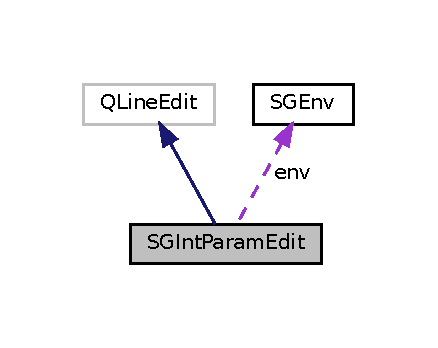
\includegraphics[width=210pt]{classSGIntParamEdit__coll__graph}
\end{center}
\end{figure}
\subsection*{Public Member Functions}
\begin{DoxyCompactItemize}
\item 
\mbox{\Hypertarget{classSGIntParamEdit_a3029714bc0bb212195a197eb7a2e68bb}\label{classSGIntParamEdit_a3029714bc0bb212195a197eb7a2e68bb}} 
\hyperlink{classSGIntParamEdit_a3029714bc0bb212195a197eb7a2e68bb}{S\+G\+Int\+Param\+Edit} (Q\+Widget $\ast$parent, \hyperlink{classSGEnv}{S\+G\+Env} $\ast$\+\_\+env, \hyperlink{namespaceSG_a031898e6fc0fa14d8590f85da9715f37}{S\+G\+::\+I\+N\+T\+\_\+\+P\+A\+R\+AM} \+\_\+param)
\begin{DoxyCompactList}\small\item\em Constructor. \end{DoxyCompactList}\end{DoxyCompactItemize}
\subsection*{Private Slots}
\begin{DoxyCompactItemize}
\item 
\mbox{\Hypertarget{classSGIntParamEdit_a15b46d944e6908ec0e1516419f522954}\label{classSGIntParamEdit_a15b46d944e6908ec0e1516419f522954}} 
void \hyperlink{classSGIntParamEdit_a15b46d944e6908ec0e1516419f522954}{change\+Param} (const Q\+String \&text)
\begin{DoxyCompactList}\small\item\em Slot called when the Q\+Line\+Edit is edited. \end{DoxyCompactList}\item 
\mbox{\Hypertarget{classSGIntParamEdit_ac9e1dba5585ebc921169deee8373a9c9}\label{classSGIntParamEdit_ac9e1dba5585ebc921169deee8373a9c9}} 
void \hyperlink{classSGIntParamEdit_ac9e1dba5585ebc921169deee8373a9c9}{reset\+Param} ()
\begin{DoxyCompactList}\small\item\em Slot called when resetting to default values. \end{DoxyCompactList}\end{DoxyCompactItemize}
\subsection*{Private Attributes}
\begin{DoxyCompactItemize}
\item 
\mbox{\Hypertarget{classSGIntParamEdit_aa1ab1c2b663dc61f85a1c137dac64841}\label{classSGIntParamEdit_aa1ab1c2b663dc61f85a1c137dac64841}} 
\hyperlink{namespaceSG_a031898e6fc0fa14d8590f85da9715f37}{S\+G\+::\+I\+N\+T\+\_\+\+P\+A\+R\+AM} \hyperlink{classSGIntParamEdit_aa1ab1c2b663dc61f85a1c137dac64841}{param}
\begin{DoxyCompactList}\small\item\em The int parameter associated with this edit. \end{DoxyCompactList}\item 
\mbox{\Hypertarget{classSGIntParamEdit_a0ecae58e72b1779e5fb99409e53f2797}\label{classSGIntParamEdit_a0ecae58e72b1779e5fb99409e53f2797}} 
\hyperlink{classSGEnv}{S\+G\+Env} $\ast$ \hyperlink{classSGIntParamEdit_a0ecae58e72b1779e5fb99409e53f2797}{env}
\begin{DoxyCompactList}\small\item\em The associated \hyperlink{classSGEnv}{S\+G\+Env} object. \end{DoxyCompactList}\end{DoxyCompactItemize}


\subsection{Detailed Description}
Class for changing integer parameters. 

A customized version of Q\+Line\+Edit for modifying int parameters in an \hyperlink{classSGEnv}{S\+G\+Env} object that is used by the \hyperlink{classSGSettingsHandler}{S\+G\+Settings\+Handler}. It has a private members which are the particular \hyperlink{namespaceSG_a031898e6fc0fa14d8590f85da9715f37}{S\+G\+::\+I\+N\+T\+\_\+\+P\+A\+R\+AM} that is associated with this edit and a pointer to an associated \hyperlink{classSGEnv}{S\+G\+Env} object. There are also mutator methods for setting the parameter value and resetting to the default value of the given parameter. 

The documentation for this class was generated from the following file\+:\begin{DoxyCompactItemize}
\item 
viewer/hpp/sgsettingshandler.\+hpp\end{DoxyCompactItemize}

\hypertarget{classSGIteration}{}\section{S\+G\+Iteration Class Reference}
\label{classSGIteration}\index{S\+G\+Iteration@{S\+G\+Iteration}}


Stores data on the behavior of \hyperlink{classSGApprox_a9cf7330f7cab3f454b0850e778d132fa}{S\+G\+Approx\+::generate()}  




{\ttfamily \#include $<$sgiteration.\+hpp$>$}



Collaboration diagram for S\+G\+Iteration\+:
\nopagebreak
\begin{figure}[H]
\begin{center}
\leavevmode
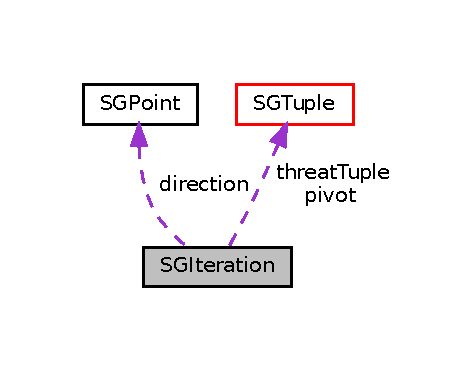
\includegraphics[width=228pt]{classSGIteration__coll__graph}
\end{center}
\end{figure}
\subsection*{Public Member Functions}
\begin{DoxyCompactItemize}
\item 
\mbox{\Hypertarget{classSGIteration_aa47645b3a728b2ca55ad2e7d17c5c488}\label{classSGIteration_aa47645b3a728b2ca55ad2e7d17c5c488}} 
\hyperlink{classSGIteration_aa47645b3a728b2ca55ad2e7d17c5c488}{S\+G\+Iteration} ()
\begin{DoxyCompactList}\small\item\em Default constructor. \end{DoxyCompactList}\item 
\hyperlink{classSGIteration_a4ac425cc85882c11443ef43601efd80b}{S\+G\+Iteration} (const \hyperlink{classSGApprox}{S\+G\+Approx} \&approx, bool store\+Actions=true)
\item 
\mbox{\Hypertarget{classSGIteration_a84d8aaef35b4a93f555cf1e0d8e5b964}\label{classSGIteration_a84d8aaef35b4a93f555cf1e0d8e5b964}} 
int \hyperlink{classSGIteration_a84d8aaef35b4a93f555cf1e0d8e5b964}{get\+Iteration} () const
\begin{DoxyCompactList}\small\item\em Get method for the iteration. \end{DoxyCompactList}\item 
\mbox{\Hypertarget{classSGIteration_af8b2fc2937e7c81248009904ffd0c14b}\label{classSGIteration_af8b2fc2937e7c81248009904ffd0c14b}} 
int \hyperlink{classSGIteration_af8b2fc2937e7c81248009904ffd0c14b}{get\+Revolution} () const
\begin{DoxyCompactList}\small\item\em Get method for the revolution. \end{DoxyCompactList}\item 
\mbox{\Hypertarget{classSGIteration_afd87a05e0df65e9361044f5cef1c5cc6}\label{classSGIteration_afd87a05e0df65e9361044f5cef1c5cc6}} 
int \hyperlink{classSGIteration_afd87a05e0df65e9361044f5cef1c5cc6}{get\+Num\+Extreme\+Tuples} () const
\begin{DoxyCompactList}\small\item\em Get method for the number of extreme tuples. \end{DoxyCompactList}\item 
\mbox{\Hypertarget{classSGIteration_a4a9c13016c8f6ffd0238e95c0076011c}\label{classSGIteration_a4a9c13016c8f6ffd0238e95c0076011c}} 
const \hyperlink{classSGTuple}{S\+G\+Tuple} \& \hyperlink{classSGIteration_a4a9c13016c8f6ffd0238e95c0076011c}{get\+Pivot} () const
\begin{DoxyCompactList}\small\item\em Get method for the current pivot. \end{DoxyCompactList}\item 
\mbox{\Hypertarget{classSGIteration_a684abe31e6b4a3bdf94be1b3fdc6cc66}\label{classSGIteration_a684abe31e6b4a3bdf94be1b3fdc6cc66}} 
const \hyperlink{classSGPoint}{S\+G\+Point} \& \hyperlink{classSGIteration_a684abe31e6b4a3bdf94be1b3fdc6cc66}{get\+Direction} () const
\begin{DoxyCompactList}\small\item\em Get method for the current direction. \end{DoxyCompactList}\item 
\mbox{\Hypertarget{classSGIteration_afb42582d89f27f44d7e76a2f4ff8a684}\label{classSGIteration_afb42582d89f27f44d7e76a2f4ff8a684}} 
const vector$<$ vector$<$ \hyperlink{classSGBaseAction}{S\+G\+Base\+Action} $>$ $>$ \& \hyperlink{classSGIteration_afb42582d89f27f44d7e76a2f4ff8a684}{get\+Actions} () const
\begin{DoxyCompactList}\small\item\em Get method for the actions available at the current iteration. \end{DoxyCompactList}\item 
\mbox{\Hypertarget{classSGIteration_a68b79d82fca24ae8fd10ef1192d9a89e}\label{classSGIteration_a68b79d82fca24ae8fd10ef1192d9a89e}} 
int \hyperlink{classSGIteration_a68b79d82fca24ae8fd10ef1192d9a89e}{get\+Best\+State} () const
\begin{DoxyCompactList}\small\item\em Get method for the best state. \end{DoxyCompactList}\item 
\mbox{\Hypertarget{classSGIteration_a7ea9824327feae3242915ee676b66ae5}\label{classSGIteration_a7ea9824327feae3242915ee676b66ae5}} 
int \hyperlink{classSGIteration_a7ea9824327feae3242915ee676b66ae5}{get\+Best\+Action} () const
\begin{DoxyCompactList}\small\item\em Get method for the best action. \end{DoxyCompactList}\item 
\mbox{\Hypertarget{classSGIteration_a6495e67cc2fd614335416e50aa725955}\label{classSGIteration_a6495e67cc2fd614335416e50aa725955}} 
\hyperlink{namespaceSG_a139e4dec41ea0f38aae1f93f60cfff60}{S\+G\+::\+Regime} \hyperlink{classSGIteration_a6495e67cc2fd614335416e50aa725955}{get\+Regime} () const
\begin{DoxyCompactList}\small\item\em Get method for the regime corresponding to the best direction. \end{DoxyCompactList}\item 
\mbox{\Hypertarget{classSGIteration_a2b8d87df8e7c5cc825938c0f57368c21}\label{classSGIteration_a2b8d87df8e7c5cc825938c0f57368c21}} 
const vector$<$ int $>$ \& \hyperlink{classSGIteration_a2b8d87df8e7c5cc825938c0f57368c21}{get\+Action\+Tuple} () const
\begin{DoxyCompactList}\small\item\em Get method for the action tuple. \end{DoxyCompactList}\item 
\mbox{\Hypertarget{classSGIteration_aefc7abf8f1819c34acf04f313d8908d2}\label{classSGIteration_aefc7abf8f1819c34acf04f313d8908d2}} 
const vector$<$ \hyperlink{namespaceSG_a139e4dec41ea0f38aae1f93f60cfff60}{S\+G\+::\+Regime} $>$ \& \hyperlink{classSGIteration_aefc7abf8f1819c34acf04f313d8908d2}{get\+Regime\+Tuple} () const
\begin{DoxyCompactList}\small\item\em Get method for the regime tuple. \end{DoxyCompactList}\item 
\mbox{\Hypertarget{classSGIteration_a1480e56c07b27be906de438b105945da}\label{classSGIteration_a1480e56c07b27be906de438b105945da}} 
const \hyperlink{classSGTuple}{S\+G\+Tuple} \& \hyperlink{classSGIteration_a1480e56c07b27be906de438b105945da}{get\+Threat\+Tuple} () const
\begin{DoxyCompactList}\small\item\em Get method for the current threat tuple. \end{DoxyCompactList}\item 
\mbox{\Hypertarget{classSGIteration_a19860e6d2af702df4ce47e36d4d43ec5}\label{classSGIteration_a19860e6d2af702df4ce47e36d4d43ec5}} 
{\footnotesize template$<$class Archive $>$ }\\void \hyperlink{classSGIteration_a19860e6d2af702df4ce47e36d4d43ec5}{serialize} (Archive \&ar, const unsigned int version)
\begin{DoxyCompactList}\small\item\em Serialize the iteration using Boost. \end{DoxyCompactList}\end{DoxyCompactItemize}
\subsection*{Private Attributes}
\begin{DoxyCompactItemize}
\item 
int \hyperlink{classSGIteration_a44a4f9e3cb074181292ae816b2c28d9e}{iteration}
\item 
int \hyperlink{classSGIteration_a21cc5c4fc7c40ff444ac7e3743c13940}{revolution}
\item 
int \hyperlink{classSGIteration_a14ecfb94b3111911d9b0ef545f72e88d}{num\+Extreme\+Tuples}
\item 
\hyperlink{classSGTuple}{S\+G\+Tuple} \hyperlink{classSGIteration_abdae7d336968af3515e7d9590cbcc46d}{pivot}
\item 
\hyperlink{classSGPoint}{S\+G\+Point} \hyperlink{classSGIteration_ac35e7e3049cd60c695a366cb8f75db37}{direction}
\item 
vector$<$ vector$<$ \hyperlink{classSGBaseAction}{S\+G\+Base\+Action} $>$ $>$ \hyperlink{classSGIteration_a5b5fcd6440b8dbcc6a8ded9f81699337}{actions}
\item 
\mbox{\Hypertarget{classSGIteration_a16f16d027bab6baffeee1f4cadb3ce8f}\label{classSGIteration_a16f16d027bab6baffeee1f4cadb3ce8f}} 
int \hyperlink{classSGIteration_a16f16d027bab6baffeee1f4cadb3ce8f}{best\+State}
\begin{DoxyCompactList}\small\item\em The state that generated the best direction. \end{DoxyCompactList}\item 
\mbox{\Hypertarget{classSGIteration_a71c4414688b49fe6205fe8d90febd5b5}\label{classSGIteration_a71c4414688b49fe6205fe8d90febd5b5}} 
int \hyperlink{classSGIteration_a71c4414688b49fe6205fe8d90febd5b5}{best\+Action}
\begin{DoxyCompactList}\small\item\em The action that generated the best direction. \end{DoxyCompactList}\item 
\mbox{\Hypertarget{classSGIteration_a0dae9bbd62ac96335698290c2866efc8}\label{classSGIteration_a0dae9bbd62ac96335698290c2866efc8}} 
\hyperlink{namespaceSG_a139e4dec41ea0f38aae1f93f60cfff60}{S\+G\+::\+Regime} \hyperlink{classSGIteration_a0dae9bbd62ac96335698290c2866efc8}{regime}
\begin{DoxyCompactList}\small\item\em True if the best direction was non-\/binding. \end{DoxyCompactList}\item 
\mbox{\Hypertarget{classSGIteration_ade2d5d602a23f5a83a76283fa4dcec87}\label{classSGIteration_ade2d5d602a23f5a83a76283fa4dcec87}} 
vector$<$ int $>$ \hyperlink{classSGIteration_ade2d5d602a23f5a83a76283fa4dcec87}{action\+Tuple}
\begin{DoxyCompactList}\small\item\em The current action tuple. \end{DoxyCompactList}\item 
\mbox{\Hypertarget{classSGIteration_a81c6328aac47bae67d8d7fdd175af738}\label{classSGIteration_a81c6328aac47bae67d8d7fdd175af738}} 
vector$<$ \hyperlink{namespaceSG_a139e4dec41ea0f38aae1f93f60cfff60}{S\+G\+::\+Regime} $>$ \hyperlink{classSGIteration_a81c6328aac47bae67d8d7fdd175af738}{regime\+Tuple}
\begin{DoxyCompactList}\small\item\em The states in which IC constraints are not binding. \end{DoxyCompactList}\item 
\mbox{\Hypertarget{classSGIteration_acaf191aa3e5adddbf1052602c927d03f}\label{classSGIteration_acaf191aa3e5adddbf1052602c927d03f}} 
\hyperlink{classSGTuple}{S\+G\+Tuple} \hyperlink{classSGIteration_acaf191aa3e5adddbf1052602c927d03f}{threat\+Tuple}
\begin{DoxyCompactList}\small\item\em The current threat tuple. \end{DoxyCompactList}\end{DoxyCompactItemize}
\subsection*{Friends}
\begin{DoxyCompactItemize}
\item 
\mbox{\Hypertarget{classSGIteration_ac98d07dd8f7b70e16ccb9a01abf56b9c}\label{classSGIteration_ac98d07dd8f7b70e16ccb9a01abf56b9c}} 
class \hyperlink{classSGIteration_ac98d07dd8f7b70e16ccb9a01abf56b9c}{boost\+::serialization\+::access}
\begin{DoxyCompactList}\small\item\em Serializes the \hyperlink{classSGIteration}{S\+G\+Iteration} object using boost. \end{DoxyCompactList}\end{DoxyCompactItemize}


\subsection{Detailed Description}
Stores data on the behavior of \hyperlink{classSGApprox_a9cf7330f7cab3f454b0850e778d132fa}{S\+G\+Approx\+::generate()} 

This class records information on each cut made by the twist algorithm.

Part of the pencil sharpening algorithm. 

\subsection{Constructor \& Destructor Documentation}
\mbox{\Hypertarget{classSGIteration_a4ac425cc85882c11443ef43601efd80b}\label{classSGIteration_a4ac425cc85882c11443ef43601efd80b}} 
\index{S\+G\+Iteration@{S\+G\+Iteration}!S\+G\+Iteration@{S\+G\+Iteration}}
\index{S\+G\+Iteration@{S\+G\+Iteration}!S\+G\+Iteration@{S\+G\+Iteration}}
\subsubsection{\texorpdfstring{S\+G\+Iteration()}{SGIteration()}}
{\footnotesize\ttfamily S\+G\+Iteration\+::\+S\+G\+Iteration (\begin{DoxyParamCaption}\item[{const \hyperlink{classSGApprox}{S\+G\+Approx} \&}]{approx,  }\item[{bool}]{store\+Actions = {\ttfamily true} }\end{DoxyParamCaption})}

Initializes a new \hyperlink{classSGIteration}{S\+G\+Iteration} object with data on the current iteration

By default, the constructor will also copy the data in \hyperlink{classSGApprox_a0fccecf0f5dbe7e9288e47182f180879}{S\+G\+Approx\+::actions}, so that the user can later recover the test directions that were available at the given iteration. If the second argument is false, then these actions will not be stored. For large games, storing the actions can take a large amount of memory. 

\subsection{Member Data Documentation}
\mbox{\Hypertarget{classSGIteration_a5b5fcd6440b8dbcc6a8ded9f81699337}\label{classSGIteration_a5b5fcd6440b8dbcc6a8ded9f81699337}} 
\index{S\+G\+Iteration@{S\+G\+Iteration}!actions@{actions}}
\index{actions@{actions}!S\+G\+Iteration@{S\+G\+Iteration}}
\subsubsection{\texorpdfstring{actions}{actions}}
{\footnotesize\ttfamily vector$<$ vector$<$\hyperlink{classSGBaseAction}{S\+G\+Base\+Action}$>$ $>$ S\+G\+Iteration\+::actions\hspace{0.3cm}{\ttfamily [private]}}

The actions that can be supported at the current iteration \mbox{\Hypertarget{classSGIteration_ac35e7e3049cd60c695a366cb8f75db37}\label{classSGIteration_ac35e7e3049cd60c695a366cb8f75db37}} 
\index{S\+G\+Iteration@{S\+G\+Iteration}!direction@{direction}}
\index{direction@{direction}!S\+G\+Iteration@{S\+G\+Iteration}}
\subsubsection{\texorpdfstring{direction}{direction}}
{\footnotesize\ttfamily \hyperlink{classSGPoint}{S\+G\+Point} S\+G\+Iteration\+::direction\hspace{0.3cm}{\ttfamily [private]}}

The shallowest admissible direction at the current revolution. \mbox{\Hypertarget{classSGIteration_a44a4f9e3cb074181292ae816b2c28d9e}\label{classSGIteration_a44a4f9e3cb074181292ae816b2c28d9e}} 
\index{S\+G\+Iteration@{S\+G\+Iteration}!iteration@{iteration}}
\index{iteration@{iteration}!S\+G\+Iteration@{S\+G\+Iteration}}
\subsubsection{\texorpdfstring{iteration}{iteration}}
{\footnotesize\ttfamily int S\+G\+Iteration\+::iteration\hspace{0.3cm}{\ttfamily [private]}}

The value of \hyperlink{classSGApprox_a7ab53424f5933726a15001ff2885a4a9}{S\+G\+Approx\+::num\+Iterations}. \mbox{\Hypertarget{classSGIteration_a14ecfb94b3111911d9b0ef545f72e88d}\label{classSGIteration_a14ecfb94b3111911d9b0ef545f72e88d}} 
\index{S\+G\+Iteration@{S\+G\+Iteration}!num\+Extreme\+Tuples@{num\+Extreme\+Tuples}}
\index{num\+Extreme\+Tuples@{num\+Extreme\+Tuples}!S\+G\+Iteration@{S\+G\+Iteration}}
\subsubsection{\texorpdfstring{num\+Extreme\+Tuples}{numExtremeTuples}}
{\footnotesize\ttfamily int S\+G\+Iteration\+::num\+Extreme\+Tuples\hspace{0.3cm}{\ttfamily [private]}}

The size of \hyperlink{classSGApprox_ab0e2c4678401f806922ac64667ad5ff6}{S\+G\+Approx\+::extreme\+Tuples}. \mbox{\Hypertarget{classSGIteration_abdae7d336968af3515e7d9590cbcc46d}\label{classSGIteration_abdae7d336968af3515e7d9590cbcc46d}} 
\index{S\+G\+Iteration@{S\+G\+Iteration}!pivot@{pivot}}
\index{pivot@{pivot}!S\+G\+Iteration@{S\+G\+Iteration}}
\subsubsection{\texorpdfstring{pivot}{pivot}}
{\footnotesize\ttfamily \hyperlink{classSGTuple}{S\+G\+Tuple} S\+G\+Iteration\+::pivot\hspace{0.3cm}{\ttfamily [private]}}

The current value of \hyperlink{classSGApprox_a037c73ff2b6ff8a55fadf57bb0a6a546}{S\+G\+Approx\+::pivot}. \mbox{\Hypertarget{classSGIteration_a21cc5c4fc7c40ff444ac7e3743c13940}\label{classSGIteration_a21cc5c4fc7c40ff444ac7e3743c13940}} 
\index{S\+G\+Iteration@{S\+G\+Iteration}!revolution@{revolution}}
\index{revolution@{revolution}!S\+G\+Iteration@{S\+G\+Iteration}}
\subsubsection{\texorpdfstring{revolution}{revolution}}
{\footnotesize\ttfamily int S\+G\+Iteration\+::revolution\hspace{0.3cm}{\ttfamily [private]}}

The value of \hyperlink{classSGApprox_a2bd0cab80a3f8d799fdc2841b65dd2c2}{S\+G\+Approx\+::num\+Revolutions}. 

The documentation for this class was generated from the following files\+:\begin{DoxyCompactItemize}
\item 
src/hpp/sgiteration.\+hpp\item 
src/cpp/sgiteration.\+cpp\end{DoxyCompactItemize}

\hypertarget{classSGIteration__MaxMinMax}{}\section{S\+G\+Iteration\+\_\+\+Max\+Min\+Max Class Reference}
\label{classSGIteration__MaxMinMax}\index{S\+G\+Iteration\+\_\+\+Max\+Min\+Max@{S\+G\+Iteration\+\_\+\+Max\+Min\+Max}}


Stores data on the behavior of \hyperlink{classSGSolver__MaxMinMax}{S\+G\+Solver\+\_\+\+Max\+Min\+Max}.  




{\ttfamily \#include $<$sgiteration\+\_\+maxminmax.\+hpp$>$}



Collaboration diagram for S\+G\+Iteration\+\_\+\+Max\+Min\+Max\+:
\nopagebreak
\begin{figure}[H]
\begin{center}
\leavevmode
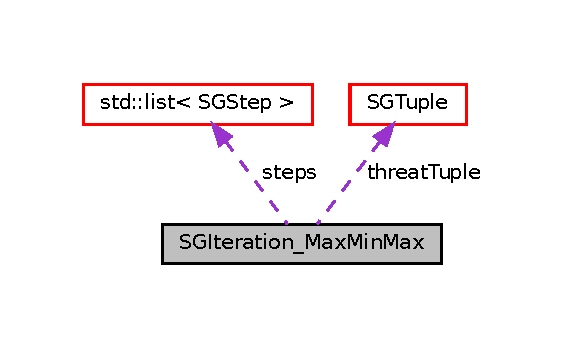
\includegraphics[width=271pt]{classSGIteration__MaxMinMax__coll__graph}
\end{center}
\end{figure}
\subsection*{Public Member Functions}
\begin{DoxyCompactItemize}
\item 
\mbox{\Hypertarget{classSGIteration__MaxMinMax_ad1b8626f55b8bf7bc1bf5d1d248d3434}\label{classSGIteration__MaxMinMax_ad1b8626f55b8bf7bc1bf5d1d248d3434}} 
\hyperlink{classSGIteration__MaxMinMax_ad1b8626f55b8bf7bc1bf5d1d248d3434}{S\+G\+Iteration\+\_\+\+Max\+Min\+Max} ()
\begin{DoxyCompactList}\small\item\em Default constructor. \end{DoxyCompactList}\item 
\hyperlink{classSGIteration__MaxMinMax_ab30ded06cb025b502da9f9b2354f9e05}{S\+G\+Iteration\+\_\+\+Max\+Min\+Max} (const vector$<$ list$<$ \hyperlink{classSGAction__MaxMinMax}{S\+G\+Action\+\_\+\+Max\+Min\+Max} $>$ $>$ \&\+\_\+actions, const \hyperlink{classSGTuple}{S\+G\+Tuple} \&\+\_\+threat\+Tuple)
\item 
\mbox{\Hypertarget{classSGIteration__MaxMinMax_a09973d8b9e68b2c58c352e012750ea88}\label{classSGIteration__MaxMinMax_a09973d8b9e68b2c58c352e012750ea88}} 
void \hyperlink{classSGIteration__MaxMinMax_a09973d8b9e68b2c58c352e012750ea88}{push\+\_\+back} (const \hyperlink{classSGStep}{S\+G\+Step} \&step)
\begin{DoxyCompactList}\small\item\em Add an \hyperlink{classSGStep}{S\+G\+Step}. \end{DoxyCompactList}\item 
\mbox{\Hypertarget{classSGIteration__MaxMinMax_a5183c9cf3aecf12250b657a34283e1fb}\label{classSGIteration__MaxMinMax_a5183c9cf3aecf12250b657a34283e1fb}} 
const list$<$ \hyperlink{classSGStep}{S\+G\+Step} $>$ \& \hyperlink{classSGIteration__MaxMinMax_a5183c9cf3aecf12250b657a34283e1fb}{get\+Steps} () const
\begin{DoxyCompactList}\small\item\em Get method for the steps. \end{DoxyCompactList}\item 
\mbox{\Hypertarget{classSGIteration__MaxMinMax_ab7935dfd6cfc657723279e1570264e28}\label{classSGIteration__MaxMinMax_ab7935dfd6cfc657723279e1570264e28}} 
const vector$<$ vector$<$ \hyperlink{classSGBaseAction}{S\+G\+Base\+Action} $>$ $>$ \& \hyperlink{classSGIteration__MaxMinMax_ab7935dfd6cfc657723279e1570264e28}{get\+Actions} () const
\begin{DoxyCompactList}\small\item\em Get method for the actions available at the current iteration. \end{DoxyCompactList}\item 
\mbox{\Hypertarget{classSGIteration__MaxMinMax_aca2ec19eb2806af69fdd7c7121794d04}\label{classSGIteration__MaxMinMax_aca2ec19eb2806af69fdd7c7121794d04}} 
const \hyperlink{classSGTuple}{S\+G\+Tuple} \& \hyperlink{classSGIteration__MaxMinMax_aca2ec19eb2806af69fdd7c7121794d04}{get\+Threat\+Tuple} () const
\begin{DoxyCompactList}\small\item\em Get method for the current threat tuple. \end{DoxyCompactList}\item 
\mbox{\Hypertarget{classSGIteration__MaxMinMax_ae5590462f3a8b5b378a7ee35ffb8fcb0}\label{classSGIteration__MaxMinMax_ae5590462f3a8b5b378a7ee35ffb8fcb0}} 
{\footnotesize template$<$class Archive $>$ }\\void \hyperlink{classSGIteration__MaxMinMax_ae5590462f3a8b5b378a7ee35ffb8fcb0}{serialize} (Archive \&ar, const unsigned int version)
\begin{DoxyCompactList}\small\item\em Serialize the iteration using Boost. \end{DoxyCompactList}\end{DoxyCompactItemize}
\subsection*{Private Attributes}
\begin{DoxyCompactItemize}
\item 
vector$<$ vector$<$ \hyperlink{classSGBaseAction}{S\+G\+Base\+Action} $>$ $>$ \hyperlink{classSGIteration__MaxMinMax_a0f6a9b1c5590ba858e154f365c09b472}{actions}
\item 
\hyperlink{classSGTuple}{S\+G\+Tuple} \hyperlink{classSGIteration__MaxMinMax_a095e196445f8ade3f0da2715b2337cae}{threat\+Tuple}
\item 
list$<$ \hyperlink{classSGStep}{S\+G\+Step} $>$ \hyperlink{classSGIteration__MaxMinMax_aba082a06c4a9bf9c1f1dcc70ae159838}{steps}
\end{DoxyCompactItemize}
\subsection*{Friends}
\begin{DoxyCompactItemize}
\item 
\mbox{\Hypertarget{classSGIteration__MaxMinMax_ac98d07dd8f7b70e16ccb9a01abf56b9c}\label{classSGIteration__MaxMinMax_ac98d07dd8f7b70e16ccb9a01abf56b9c}} 
class \hyperlink{classSGIteration__MaxMinMax_ac98d07dd8f7b70e16ccb9a01abf56b9c}{boost\+::serialization\+::access}
\begin{DoxyCompactList}\small\item\em Serializes the \hyperlink{classSGIteration__MaxMinMax}{S\+G\+Iteration\+\_\+\+Max\+Min\+Max} object using boost. \end{DoxyCompactList}\end{DoxyCompactItemize}


\subsection{Detailed Description}
Stores data on the behavior of \hyperlink{classSGSolver__MaxMinMax}{S\+G\+Solver\+\_\+\+Max\+Min\+Max}. 

This class records the status of the max-\/min-\/max algorithm after each implementation of the max-\/min-\/max operator. 

\subsection{Constructor \& Destructor Documentation}
\mbox{\Hypertarget{classSGIteration__MaxMinMax_ab30ded06cb025b502da9f9b2354f9e05}\label{classSGIteration__MaxMinMax_ab30ded06cb025b502da9f9b2354f9e05}} 
\index{S\+G\+Iteration\+\_\+\+Max\+Min\+Max@{S\+G\+Iteration\+\_\+\+Max\+Min\+Max}!S\+G\+Iteration\+\_\+\+Max\+Min\+Max@{S\+G\+Iteration\+\_\+\+Max\+Min\+Max}}
\index{S\+G\+Iteration\+\_\+\+Max\+Min\+Max@{S\+G\+Iteration\+\_\+\+Max\+Min\+Max}!S\+G\+Iteration\+\_\+\+Max\+Min\+Max@{S\+G\+Iteration\+\_\+\+Max\+Min\+Max}}
\subsubsection{\texorpdfstring{S\+G\+Iteration\+\_\+\+Max\+Min\+Max()}{SGIteration\_MaxMinMax()}}
{\footnotesize\ttfamily S\+G\+Iteration\+\_\+\+Max\+Min\+Max\+::\+S\+G\+Iteration\+\_\+\+Max\+Min\+Max (\begin{DoxyParamCaption}\item[{const vector$<$ list$<$ \hyperlink{classSGAction__MaxMinMax}{S\+G\+Action\+\_\+\+Max\+Min\+Max} $>$ $>$ \&}]{\+\_\+actions,  }\item[{const \hyperlink{classSGTuple}{S\+G\+Tuple} \&}]{\+\_\+threat\+Tuple }\end{DoxyParamCaption})\hspace{0.3cm}{\ttfamily [inline]}}

Initializes a new \hyperlink{classSGIteration__MaxMinMax}{S\+G\+Iteration\+\_\+\+Max\+Min\+Max} object with data on the current iteration

The constructor will copy the data in \hyperlink{classSGSolver__MaxMinMax_ad1a4bf22aaa58dd05c7bc7a24d9c1805}{S\+G\+Solver\+\_\+\+Max\+Min\+Max\+::actions}, so that the user can later recover the test directions that were available at each step. For large games, storing the actions can take a large amount of memory. 

\subsection{Member Data Documentation}
\mbox{\Hypertarget{classSGIteration__MaxMinMax_a0f6a9b1c5590ba858e154f365c09b472}\label{classSGIteration__MaxMinMax_a0f6a9b1c5590ba858e154f365c09b472}} 
\index{S\+G\+Iteration\+\_\+\+Max\+Min\+Max@{S\+G\+Iteration\+\_\+\+Max\+Min\+Max}!actions@{actions}}
\index{actions@{actions}!S\+G\+Iteration\+\_\+\+Max\+Min\+Max@{S\+G\+Iteration\+\_\+\+Max\+Min\+Max}}
\subsubsection{\texorpdfstring{actions}{actions}}
{\footnotesize\ttfamily vector$<$ vector$<$\hyperlink{classSGBaseAction}{S\+G\+Base\+Action}$>$ $>$ S\+G\+Iteration\+\_\+\+Max\+Min\+Max\+::actions\hspace{0.3cm}{\ttfamily [private]}}

The actions that can be supported at the current iteration \mbox{\Hypertarget{classSGIteration__MaxMinMax_aba082a06c4a9bf9c1f1dcc70ae159838}\label{classSGIteration__MaxMinMax_aba082a06c4a9bf9c1f1dcc70ae159838}} 
\index{S\+G\+Iteration\+\_\+\+Max\+Min\+Max@{S\+G\+Iteration\+\_\+\+Max\+Min\+Max}!steps@{steps}}
\index{steps@{steps}!S\+G\+Iteration\+\_\+\+Max\+Min\+Max@{S\+G\+Iteration\+\_\+\+Max\+Min\+Max}}
\subsubsection{\texorpdfstring{steps}{steps}}
{\footnotesize\ttfamily list$<$\hyperlink{classSGStep}{S\+G\+Step}$>$ S\+G\+Iteration\+\_\+\+Max\+Min\+Max\+::steps\hspace{0.3cm}{\ttfamily [private]}}

The steps in the iteration \mbox{\Hypertarget{classSGIteration__MaxMinMax_a095e196445f8ade3f0da2715b2337cae}\label{classSGIteration__MaxMinMax_a095e196445f8ade3f0da2715b2337cae}} 
\index{S\+G\+Iteration\+\_\+\+Max\+Min\+Max@{S\+G\+Iteration\+\_\+\+Max\+Min\+Max}!threat\+Tuple@{threat\+Tuple}}
\index{threat\+Tuple@{threat\+Tuple}!S\+G\+Iteration\+\_\+\+Max\+Min\+Max@{S\+G\+Iteration\+\_\+\+Max\+Min\+Max}}
\subsubsection{\texorpdfstring{threat\+Tuple}{threatTuple}}
{\footnotesize\ttfamily \hyperlink{classSGTuple}{S\+G\+Tuple} S\+G\+Iteration\+\_\+\+Max\+Min\+Max\+::threat\+Tuple\hspace{0.3cm}{\ttfamily [private]}}

The current threat tuple. 

The documentation for this class was generated from the following file\+:\begin{DoxyCompactItemize}
\item 
src/hpp/sgiteration\+\_\+maxminmax.\+hpp\end{DoxyCompactItemize}

\hypertarget{classSGLegend}{}\section{S\+G\+Legend Class Reference}
\label{classSGLegend}\index{S\+G\+Legend@{S\+G\+Legend}}


A class for displaying a legend for the solution plots.  




{\ttfamily \#include $<$sglegend.\+hpp$>$}



Inheritance diagram for S\+G\+Legend\+:
\nopagebreak
\begin{figure}[H]
\begin{center}
\leavevmode
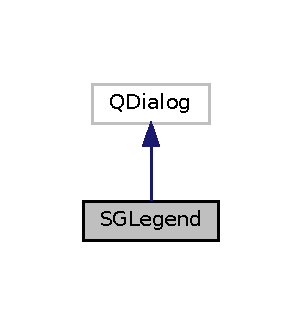
\includegraphics[width=145pt]{classSGLegend__inherit__graph}
\end{center}
\end{figure}


Collaboration diagram for S\+G\+Legend\+:
\nopagebreak
\begin{figure}[H]
\begin{center}
\leavevmode
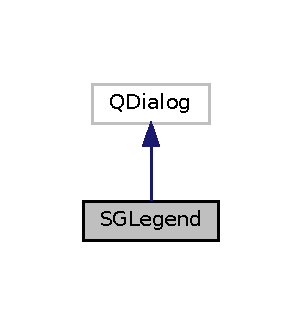
\includegraphics[width=145pt]{classSGLegend__coll__graph}
\end{center}
\end{figure}
\subsection*{Public Member Functions}
\begin{DoxyCompactItemize}
\item 
\mbox{\Hypertarget{classSGLegend_ac105f7004cae38c0834ae2e6a0920c9e}\label{classSGLegend_ac105f7004cae38c0834ae2e6a0920c9e}} 
\hyperlink{classSGLegend_ac105f7004cae38c0834ae2e6a0920c9e}{S\+G\+Legend} (Q\+Widget $\ast$parent)
\begin{DoxyCompactList}\small\item\em Constructor. \end{DoxyCompactList}\end{DoxyCompactItemize}


\subsection{Detailed Description}
A class for displaying a legend for the solution plots. 

The documentation for this class was generated from the following files\+:\begin{DoxyCompactItemize}
\item 
viewer/hpp/sglegend.\+hpp\item 
viewer/cpp/sglegend.\+cpp\end{DoxyCompactItemize}

\hypertarget{classSGMainWindow}{}\section{S\+G\+Main\+Window Class Reference}
\label{classSGMainWindow}\index{S\+G\+Main\+Window@{S\+G\+Main\+Window}}


Main window for S\+G\+Viewer.  




{\ttfamily \#include $<$sgmainwindow.\+hpp$>$}



Inheritance diagram for S\+G\+Main\+Window\+:
\nopagebreak
\begin{figure}[H]
\begin{center}
\leavevmode
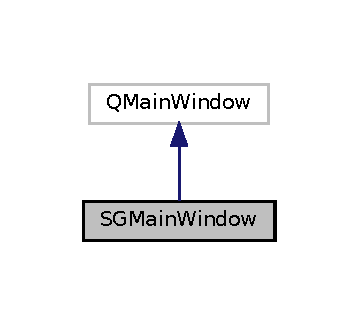
\includegraphics[width=172pt]{classSGMainWindow__inherit__graph}
\end{center}
\end{figure}


Collaboration diagram for S\+G\+Main\+Window\+:
\nopagebreak
\begin{figure}[H]
\begin{center}
\leavevmode
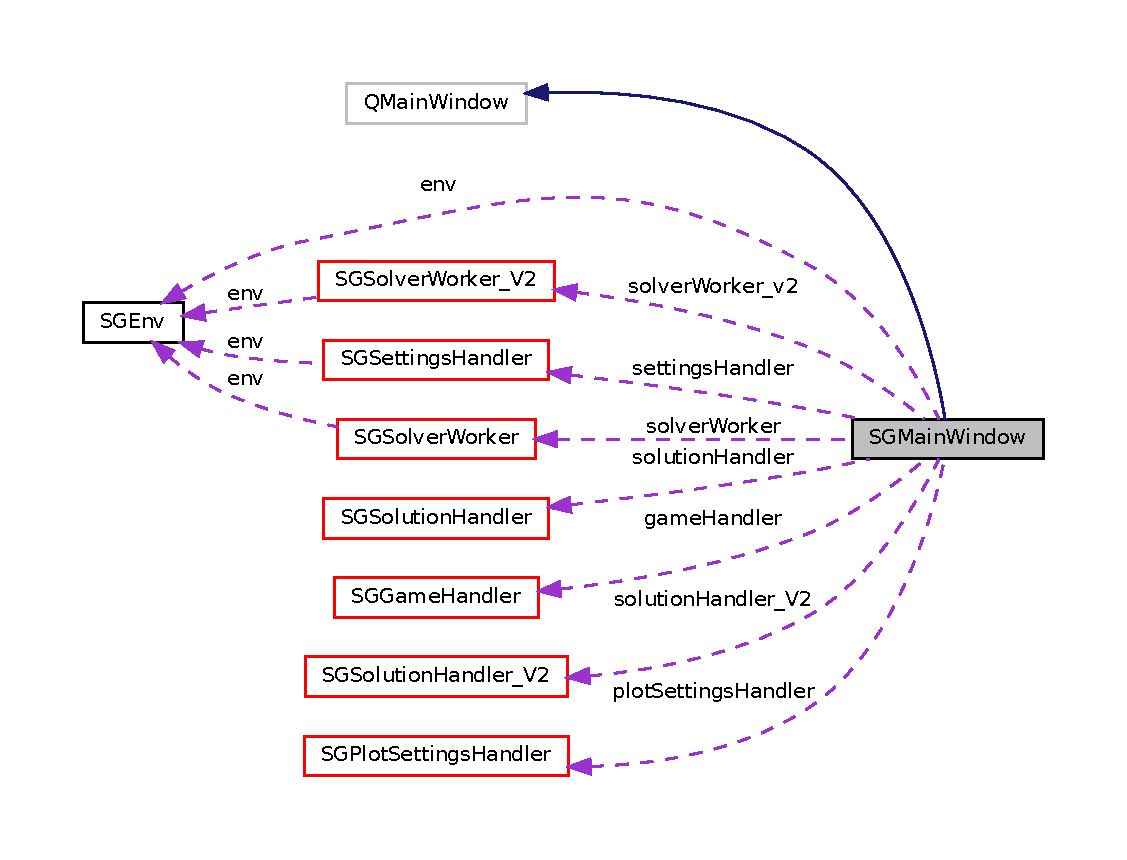
\includegraphics[width=350pt]{classSGMainWindow__coll__graph}
\end{center}
\end{figure}
\subsection*{Signals}
\begin{DoxyCompactItemize}
\item 
\mbox{\Hypertarget{classSGMainWindow_a1abe4b80ca1554d9863e53323e91847e}\label{classSGMainWindow_a1abe4b80ca1554d9863e53323e91847e}} 
void \hyperlink{classSGMainWindow_a1abe4b80ca1554d9863e53323e91847e}{start\+Iteration} ()
\begin{DoxyCompactList}\small\item\em Signal for S\+G\+Solver\+Thread to start next iteration. \end{DoxyCompactList}\item 
\mbox{\Hypertarget{classSGMainWindow_a155a779b9a5baace6092787bea27d459}\label{classSGMainWindow_a155a779b9a5baace6092787bea27d459}} 
void \hyperlink{classSGMainWindow_a155a779b9a5baace6092787bea27d459}{start\+Iteration\+\_\+\+V2} ()
\begin{DoxyCompactList}\small\item\em Signal for S\+G\+Solver\+Thread to start next iteration, V2. \end{DoxyCompactList}\end{DoxyCompactItemize}
\subsection*{Public Member Functions}
\begin{DoxyCompactItemize}
\item 
\hyperlink{classSGMainWindow_af2c1eed12335e81fbbf403557d410d28}{S\+G\+Main\+Window} ()
\begin{DoxyCompactList}\small\item\em Constructor. \end{DoxyCompactList}\item 
\hyperlink{classSGMainWindow_a38e9f6d5431f6b92c898089582b7d124}{$\sim$\+S\+G\+Main\+Window} ()
\begin{DoxyCompactList}\small\item\em Destructor. \end{DoxyCompactList}\end{DoxyCompactItemize}
\subsection*{Protected Member Functions}
\begin{DoxyCompactItemize}
\item 
\mbox{\Hypertarget{classSGMainWindow_a18bba6bdcde9ec59d0b0cd383b03980c}\label{classSGMainWindow_a18bba6bdcde9ec59d0b0cd383b03980c}} 
virtual void \hyperlink{classSGMainWindow_a18bba6bdcde9ec59d0b0cd383b03980c}{key\+Press\+Event} (Q\+Key\+Event $\ast$event)
\begin{DoxyCompactList}\small\item\em Handles keyboard shortcuts. \end{DoxyCompactList}\end{DoxyCompactItemize}
\subsection*{Private Slots}
\begin{DoxyCompactItemize}
\item 
\mbox{\Hypertarget{classSGMainWindow_a74ae1cc511290e9d4818ba2880970ce6}\label{classSGMainWindow_a74ae1cc511290e9d4818ba2880970ce6}} 
void \hyperlink{classSGMainWindow_a74ae1cc511290e9d4818ba2880970ce6}{load\+Solution} ()
\begin{DoxyCompactList}\small\item\em Triggers a solution load. \end{DoxyCompactList}\item 
\mbox{\Hypertarget{classSGMainWindow_a2f015bd10f6562f30efbafab51de82b6}\label{classSGMainWindow_a2f015bd10f6562f30efbafab51de82b6}} 
void \hyperlink{classSGMainWindow_a2f015bd10f6562f30efbafab51de82b6}{load\+Solution\+\_\+\+V2} ()
\begin{DoxyCompactList}\small\item\em Triggers a S\+G\+Solution\+\_\+\+V2 load. \end{DoxyCompactList}\item 
\mbox{\Hypertarget{classSGMainWindow_ac098f548f9fcbc2e19eddbe60a90db2d}\label{classSGMainWindow_ac098f548f9fcbc2e19eddbe60a90db2d}} 
void \hyperlink{classSGMainWindow_ac098f548f9fcbc2e19eddbe60a90db2d}{save\+Solution} ()
\begin{DoxyCompactList}\small\item\em Triggers a solution save. \end{DoxyCompactList}\item 
\mbox{\Hypertarget{classSGMainWindow_a8172c6ee9e3112f3f5cdcc01896c6975}\label{classSGMainWindow_a8172c6ee9e3112f3f5cdcc01896c6975}} 
void \hyperlink{classSGMainWindow_a8172c6ee9e3112f3f5cdcc01896c6975}{load\+Game} ()
\begin{DoxyCompactList}\small\item\em Triggers a game load. \end{DoxyCompactList}\item 
\mbox{\Hypertarget{classSGMainWindow_ae1561288ed4562965fca780b15fbc730}\label{classSGMainWindow_ae1561288ed4562965fca780b15fbc730}} 
void \hyperlink{classSGMainWindow_ae1561288ed4562965fca780b15fbc730}{save\+Game} ()
\begin{DoxyCompactList}\small\item\em Triggers a game save. \end{DoxyCompactList}\item 
\mbox{\Hypertarget{classSGMainWindow_a1f70e342154873b8c5254f21ec2a7883}\label{classSGMainWindow_a1f70e342154873b8c5254f21ec2a7883}} 
void \hyperlink{classSGMainWindow_a1f70e342154873b8c5254f21ec2a7883}{quit\+Program} ()
\begin{DoxyCompactList}\small\item\em Quits the program. \end{DoxyCompactList}\item 
\mbox{\Hypertarget{classSGMainWindow_a318de5525d2d88cb6bb4976ab40d9dbc}\label{classSGMainWindow_a318de5525d2d88cb6bb4976ab40d9dbc}} 
void \hyperlink{classSGMainWindow_a318de5525d2d88cb6bb4976ab40d9dbc}{change\+Settings} ()
\begin{DoxyCompactList}\small\item\em Changes settings for the \hyperlink{classSGEnv}{S\+G\+Env} object. \end{DoxyCompactList}\item 
\mbox{\Hypertarget{classSGMainWindow_a98bc00f752d14d10f4d36304ef2ffffe}\label{classSGMainWindow_a98bc00f752d14d10f4d36304ef2ffffe}} 
void \hyperlink{classSGMainWindow_a98bc00f752d14d10f4d36304ef2ffffe}{settings\+Handler\+Closed} ()
\begin{DoxyCompactList}\small\item\em Changes settings for the \hyperlink{classSGEnv}{S\+G\+Env} object. \end{DoxyCompactList}\item 
\mbox{\Hypertarget{classSGMainWindow_a96c1951da5706cddbb3c7c04642d0516}\label{classSGMainWindow_a96c1951da5706cddbb3c7c04642d0516}} 
void \hyperlink{classSGMainWindow_a96c1951da5706cddbb3c7c04642d0516}{change\+Plot\+Settings} ()
\begin{DoxyCompactList}\small\item\em Changes plot settings. \end{DoxyCompactList}\item 
\mbox{\Hypertarget{classSGMainWindow_af7b4a5dc1a931885cdb618d8fe475f02}\label{classSGMainWindow_af7b4a5dc1a931885cdb618d8fe475f02}} 
void \hyperlink{classSGMainWindow_af7b4a5dc1a931885cdb618d8fe475f02}{plot\+Settings\+Handler\+Closed} ()
\begin{DoxyCompactList}\small\item\em Changes plot settings. \end{DoxyCompactList}\item 
\mbox{\Hypertarget{classSGMainWindow_aed927310137a02965872acf8c653f39f}\label{classSGMainWindow_aed927310137a02965872acf8c653f39f}} 
void \hyperlink{classSGMainWindow_aed927310137a02965872acf8c653f39f}{screen\+Shot} ()
\begin{DoxyCompactList}\small\item\em Triggers a new screen shot. \end{DoxyCompactList}\item 
\mbox{\Hypertarget{classSGMainWindow_a35df4b379f8ee46e78771c8190188e5a}\label{classSGMainWindow_a35df4b379f8ee46e78771c8190188e5a}} 
void \hyperlink{classSGMainWindow_a35df4b379f8ee46e78771c8190188e5a}{solve\+Game} ()
\begin{DoxyCompactList}\small\item\em Initializes solve routine for pencil sharpening. \end{DoxyCompactList}\item 
\mbox{\Hypertarget{classSGMainWindow_aee37774a08e1d24544ab028d181192eb}\label{classSGMainWindow_aee37774a08e1d24544ab028d181192eb}} 
void \hyperlink{classSGMainWindow_aee37774a08e1d24544ab028d181192eb}{cancel\+Solve} ()
\begin{DoxyCompactList}\small\item\em Throws the cancel solution flag. \end{DoxyCompactList}\item 
void \hyperlink{classSGMainWindow_a511aee91c2c031f7f4a9148073177f0e}{iteration\+Finished} (bool)
\begin{DoxyCompactList}\small\item\em Slot when iteration finishes. \end{DoxyCompactList}\item 
void \hyperlink{classSGMainWindow_aa7cb5fa0763b2914492fc518dd175019}{solver\+Exception} ()
\begin{DoxyCompactList}\small\item\em Triggers error message in log. \end{DoxyCompactList}\item 
\mbox{\Hypertarget{classSGMainWindow_ad03acb0ec39c884ca93102c6c23743b5}\label{classSGMainWindow_ad03acb0ec39c884ca93102c6c23743b5}} 
void \hyperlink{classSGMainWindow_ad03acb0ec39c884ca93102c6c23743b5}{solve\+Game\+\_\+\+V2} ()
\begin{DoxyCompactList}\small\item\em Initializes solve routine for A\+BS 2018. \end{DoxyCompactList}\item 
void \hyperlink{classSGMainWindow_a59248c811344a260981ea270d86d5d19}{iteration\+Finished\+\_\+\+V2} (bool)
\begin{DoxyCompactList}\small\item\em Slot when iteration finishes, V2. \end{DoxyCompactList}\item 
void \hyperlink{classSGMainWindow_a4be88c15c38bbdc162ad410b99e79c0d}{solver\+Exception\+\_\+\+V2} ()
\begin{DoxyCompactList}\small\item\em Triggers error message in log, V2. \end{DoxyCompactList}\item 
\mbox{\Hypertarget{classSGMainWindow_a7a5038dbd555a4717ac758dfcba51a33}\label{classSGMainWindow_a7a5038dbd555a4717ac758dfcba51a33}} 
void \hyperlink{classSGMainWindow_a7a5038dbd555a4717ac758dfcba51a33}{display\+About} ()
\begin{DoxyCompactList}\small\item\em Displays an about message. \end{DoxyCompactList}\item 
\mbox{\Hypertarget{classSGMainWindow_acb8c57315148c628af407ae8da6d5bb1}\label{classSGMainWindow_acb8c57315148c628af407ae8da6d5bb1}} 
void \hyperlink{classSGMainWindow_acb8c57315148c628af407ae8da6d5bb1}{display\+Legend} ()
\begin{DoxyCompactList}\small\item\em Displays a legend. \end{DoxyCompactList}\item 
\mbox{\Hypertarget{classSGMainWindow_a1f0a10bf104be430f992d33b2de6e564}\label{classSGMainWindow_a1f0a10bf104be430f992d33b2de6e564}} 
void \hyperlink{classSGMainWindow_a1f0a10bf104be430f992d33b2de6e564}{generate\+R\+SG} ()
\begin{DoxyCompactList}\small\item\em Generate risk sharing game. \end{DoxyCompactList}\item 
\mbox{\Hypertarget{classSGMainWindow_ac5fc1ea12ae702771432bb4b5840e792}\label{classSGMainWindow_ac5fc1ea12ae702771432bb4b5840e792}} 
void \hyperlink{classSGMainWindow_ac5fc1ea12ae702771432bb4b5840e792}{generate\+PD} ()
\begin{DoxyCompactList}\small\item\em Generate prisoner\textquotesingle{}s dilemma game. \end{DoxyCompactList}\item 
\mbox{\Hypertarget{classSGMainWindow_a2b7cf2dd928b163c78df0d863fa05347}\label{classSGMainWindow_a2b7cf2dd928b163c78df0d863fa05347}} 
void \hyperlink{classSGMainWindow_a2b7cf2dd928b163c78df0d863fa05347}{generate\+BoS} ()
\begin{DoxyCompactList}\small\item\em Generate a Battle of the Sexes. \end{DoxyCompactList}\end{DoxyCompactItemize}
\subsection*{Private Member Functions}
\begin{DoxyCompactItemize}
\item 
\mbox{\Hypertarget{classSGMainWindow_a576d4a2d0b9e9b077faa59d6a1db1485}\label{classSGMainWindow_a576d4a2d0b9e9b077faa59d6a1db1485}} 
void \hyperlink{classSGMainWindow_a576d4a2d0b9e9b077faa59d6a1db1485}{settings\+Loader} ()
\begin{DoxyCompactList}\small\item\em Loads saved settings. \end{DoxyCompactList}\item 
\mbox{\Hypertarget{classSGMainWindow_ab14d201c21675bd6c5fddd79a4bd15e9}\label{classSGMainWindow_ab14d201c21675bd6c5fddd79a4bd15e9}} 
void \hyperlink{classSGMainWindow_ab14d201c21675bd6c5fddd79a4bd15e9}{settings\+Saver} ()
\begin{DoxyCompactList}\small\item\em Saves settings. \end{DoxyCompactList}\end{DoxyCompactItemize}
\subsection*{Private Attributes}
\begin{DoxyCompactItemize}
\item 
\mbox{\Hypertarget{classSGMainWindow_a817d751fa6091d4b0a6f28bd2c76ce51}\label{classSGMainWindow_a817d751fa6091d4b0a6f28bd2c76ce51}} 
Q\+Tab\+Widget $\ast$ \hyperlink{classSGMainWindow_a817d751fa6091d4b0a6f28bd2c76ce51}{tab\+Widget}
\begin{DoxyCompactList}\small\item\em Widget containing game, solution, and log tabs. \end{DoxyCompactList}\item 
\mbox{\Hypertarget{classSGMainWindow_a09d1290636a995531461fb92a5d87678}\label{classSGMainWindow_a09d1290636a995531461fb92a5d87678}} 
\hyperlink{classSGEnv}{S\+G\+Env} $\ast$ \hyperlink{classSGMainWindow_a09d1290636a995531461fb92a5d87678}{env}
\begin{DoxyCompactList}\small\item\em Environment for computations. \end{DoxyCompactList}\item 
\mbox{\Hypertarget{classSGMainWindow_a1c1cef91745063c8349994394c2f4f6d}\label{classSGMainWindow_a1c1cef91745063c8349994394c2f4f6d}} 
\hyperlink{classSGSolverWorker}{S\+G\+Solver\+Worker} $\ast$ \hyperlink{classSGMainWindow_a1c1cef91745063c8349994394c2f4f6d}{solver\+Worker}
\begin{DoxyCompactList}\small\item\em Worker that handles solution. \end{DoxyCompactList}\item 
\mbox{\Hypertarget{classSGMainWindow_a5b8bebd2fc00ff1b35ca3dd22a446357}\label{classSGMainWindow_a5b8bebd2fc00ff1b35ca3dd22a446357}} 
\hyperlink{classSGSolverWorker__V2}{S\+G\+Solver\+Worker\+\_\+\+V2} $\ast$ \hyperlink{classSGMainWindow_a5b8bebd2fc00ff1b35ca3dd22a446357}{solver\+Worker\+\_\+v2}
\begin{DoxyCompactList}\small\item\em Worker that handles solution. \end{DoxyCompactList}\item 
\mbox{\Hypertarget{classSGMainWindow_a71569a2e0e90f5efd8fe3b8d43c71473}\label{classSGMainWindow_a71569a2e0e90f5efd8fe3b8d43c71473}} 
Q\+Thread \hyperlink{classSGMainWindow_a71569a2e0e90f5efd8fe3b8d43c71473}{solver\+Thread}
\begin{DoxyCompactList}\small\item\em Separate thread for running solve routines, so gui doesn\textquotesingle{}t hang. \end{DoxyCompactList}\item 
\mbox{\Hypertarget{classSGMainWindow_a0863e0ab765177721bbda61a6494a60a}\label{classSGMainWindow_a0863e0ab765177721bbda61a6494a60a}} 
\hyperlink{classSGSolutionHandler}{S\+G\+Solution\+Handler} $\ast$ \hyperlink{classSGMainWindow_a0863e0ab765177721bbda61a6494a60a}{solution\+Handler}
\begin{DoxyCompactList}\small\item\em The object for interfacing with the solution. \end{DoxyCompactList}\item 
\mbox{\Hypertarget{classSGMainWindow_ae8ef3d9c4be577f804c54fb1bccf63a2}\label{classSGMainWindow_ae8ef3d9c4be577f804c54fb1bccf63a2}} 
\hyperlink{classSGSolutionHandler__V2}{S\+G\+Solution\+Handler\+\_\+\+V2} $\ast$ \hyperlink{classSGMainWindow_ae8ef3d9c4be577f804c54fb1bccf63a2}{solution\+Handler\+\_\+\+V2}
\begin{DoxyCompactList}\small\item\em The object for interfacing with S\+G\+Solution\+\_\+\+V2. \end{DoxyCompactList}\item 
\mbox{\Hypertarget{classSGMainWindow_aac360598eca3556adf4bba2588fb5f3c}\label{classSGMainWindow_aac360598eca3556adf4bba2588fb5f3c}} 
\hyperlink{classSGGameHandler}{S\+G\+Game\+Handler} $\ast$ \hyperlink{classSGMainWindow_aac360598eca3556adf4bba2588fb5f3c}{game\+Handler}
\begin{DoxyCompactList}\small\item\em The object for interfacing with the game. \end{DoxyCompactList}\item 
\mbox{\Hypertarget{classSGMainWindow_ab29540bcb97791859537ca8da988e3fe}\label{classSGMainWindow_ab29540bcb97791859537ca8da988e3fe}} 
\hyperlink{classSGSettingsHandler}{S\+G\+Settings\+Handler} $\ast$ \hyperlink{classSGMainWindow_ab29540bcb97791859537ca8da988e3fe}{settings\+Handler}
\begin{DoxyCompactList}\small\item\em The object for controling environment settings. \end{DoxyCompactList}\item 
\mbox{\Hypertarget{classSGMainWindow_a2acf5b1f87ba1dd721fc916661c1acfe}\label{classSGMainWindow_a2acf5b1f87ba1dd721fc916661c1acfe}} 
\hyperlink{classSGPlotSettingsHandler}{S\+G\+Plot\+Settings\+Handler} $\ast$ \hyperlink{classSGMainWindow_a2acf5b1f87ba1dd721fc916661c1acfe}{plot\+Settings\+Handler}
\begin{DoxyCompactList}\small\item\em The object for controling plot settings. \end{DoxyCompactList}\item 
\mbox{\Hypertarget{classSGMainWindow_a1bd520ead9bb17f8401a730760962b37}\label{classSGMainWindow_a1bd520ead9bb17f8401a730760962b37}} 
Q\+Text\+Edit $\ast$ \hyperlink{classSGMainWindow_a1bd520ead9bb17f8401a730760962b37}{log\+Text\+Edit}
\begin{DoxyCompactList}\small\item\em Text edit containing the log output. \end{DoxyCompactList}\item 
\mbox{\Hypertarget{classSGMainWindow_a575a41f119be8c024bead46cbaefb02b}\label{classSGMainWindow_a575a41f119be8c024bead46cbaefb02b}} 
Q\+Time \hyperlink{classSGMainWindow_a575a41f119be8c024bead46cbaefb02b}{timer}
\begin{DoxyCompactList}\small\item\em Times progress of the algorithm. \end{DoxyCompactList}\item 
\mbox{\Hypertarget{classSGMainWindow_a3fecf45fb589833629f92559ac633b53}\label{classSGMainWindow_a3fecf45fb589833629f92559ac633b53}} 
bool \hyperlink{classSGMainWindow_a3fecf45fb589833629f92559ac633b53}{cancel\+Solve\+Flag}
\begin{DoxyCompactList}\small\item\em Flag for canceling solve next time an iteration finishes. \end{DoxyCompactList}\item 
\mbox{\Hypertarget{classSGMainWindow_ae750441d6f1b88af7a3f5f27e839dd8f}\label{classSGMainWindow_ae750441d6f1b88af7a3f5f27e839dd8f}} 
Q\+String \hyperlink{classSGMainWindow_ae750441d6f1b88af7a3f5f27e839dd8f}{path}
\begin{DoxyCompactList}\small\item\em Most recent path for saves/loads. \end{DoxyCompactList}\item 
\mbox{\Hypertarget{classSGMainWindow_a55c71737fb867ee33ffa8ec709c0eca3}\label{classSGMainWindow_a55c71737fb867ee33ffa8ec709c0eca3}} 
Q\+Settings $\ast$ \hyperlink{classSGMainWindow_a55c71737fb867ee33ffa8ec709c0eca3}{settings}
\begin{DoxyCompactList}\small\item\em Program settings. \end{DoxyCompactList}\end{DoxyCompactItemize}


\subsection{Detailed Description}
Main window for S\+G\+Viewer. 

This class constructs the tabs and layouts. It also contains signals and slots for handling certain high level functions, such as solving, saving, and loading saved content.

Note that rather than using \hyperlink{classSGSolver}{S\+G\+Solver}, this class essentially replicates the behavior of the \hyperlink{classSGSolver}{S\+G\+Solver} class in its solve\+Game routine. The reason is that \hyperlink{classSGSolver}{S\+G\+Solver} runs straight through. We want to provide updates in the log window as the solver proceeds, which is facilitated by running \hyperlink{classSGSolverWorker}{S\+G\+Solver\+Worker} one iteration at a time, printing the output when each revolution finishes, and then restarting the solve routine. Also allows the user to cancel a computation when the next iteration finishes. 

\subsection{Constructor \& Destructor Documentation}
\mbox{\Hypertarget{classSGMainWindow_af2c1eed12335e81fbbf403557d410d28}\label{classSGMainWindow_af2c1eed12335e81fbbf403557d410d28}} 
\index{S\+G\+Main\+Window@{S\+G\+Main\+Window}!S\+G\+Main\+Window@{S\+G\+Main\+Window}}
\index{S\+G\+Main\+Window@{S\+G\+Main\+Window}!S\+G\+Main\+Window@{S\+G\+Main\+Window}}
\subsubsection{\texorpdfstring{S\+G\+Main\+Window()}{SGMainWindow()}}
{\footnotesize\ttfamily S\+G\+Main\+Window\+::\+S\+G\+Main\+Window (\begin{DoxyParamCaption}{ }\end{DoxyParamCaption})}



Constructor. 

Initializes member objects and connects signals and slots. \mbox{\Hypertarget{classSGMainWindow_a38e9f6d5431f6b92c898089582b7d124}\label{classSGMainWindow_a38e9f6d5431f6b92c898089582b7d124}} 
\index{S\+G\+Main\+Window@{S\+G\+Main\+Window}!````~S\+G\+Main\+Window@{$\sim$\+S\+G\+Main\+Window}}
\index{````~S\+G\+Main\+Window@{$\sim$\+S\+G\+Main\+Window}!S\+G\+Main\+Window@{S\+G\+Main\+Window}}
\subsubsection{\texorpdfstring{$\sim$\+S\+G\+Main\+Window()}{~SGMainWindow()}}
{\footnotesize\ttfamily S\+G\+Main\+Window\+::$\sim$\+S\+G\+Main\+Window (\begin{DoxyParamCaption}{ }\end{DoxyParamCaption})\hspace{0.3cm}{\ttfamily [inline]}}



Destructor. 

Just closes down the solver thread. Should other objects be destroyed? 

\subsection{Member Function Documentation}
\mbox{\Hypertarget{classSGMainWindow_a511aee91c2c031f7f4a9148073177f0e}\label{classSGMainWindow_a511aee91c2c031f7f4a9148073177f0e}} 
\index{S\+G\+Main\+Window@{S\+G\+Main\+Window}!iteration\+Finished@{iteration\+Finished}}
\index{iteration\+Finished@{iteration\+Finished}!S\+G\+Main\+Window@{S\+G\+Main\+Window}}
\subsubsection{\texorpdfstring{iteration\+Finished}{iterationFinished}}
{\footnotesize\ttfamily void S\+G\+Main\+Window\+::iteration\+Finished (\begin{DoxyParamCaption}\item[{bool}]{tf }\end{DoxyParamCaption})\hspace{0.3cm}{\ttfamily [private]}, {\ttfamily [slot]}}



Slot when iteration finishes. 

Checks if the algorithm has converged or if maximum number of iterations has finished. If the algorithm has finished, plots the solution. If the algorithm has not converged and the cancel flag is false, the next iteration is started. If the cancel flag is thrown, will not trigger the next iteration. \mbox{\Hypertarget{classSGMainWindow_a59248c811344a260981ea270d86d5d19}\label{classSGMainWindow_a59248c811344a260981ea270d86d5d19}} 
\index{S\+G\+Main\+Window@{S\+G\+Main\+Window}!iteration\+Finished\+\_\+\+V2@{iteration\+Finished\+\_\+\+V2}}
\index{iteration\+Finished\+\_\+\+V2@{iteration\+Finished\+\_\+\+V2}!S\+G\+Main\+Window@{S\+G\+Main\+Window}}
\subsubsection{\texorpdfstring{iteration\+Finished\+\_\+\+V2}{iterationFinished\_V2}}
{\footnotesize\ttfamily void S\+G\+Main\+Window\+::iteration\+Finished\+\_\+\+V2 (\begin{DoxyParamCaption}\item[{bool}]{tf }\end{DoxyParamCaption})\hspace{0.3cm}{\ttfamily [private]}, {\ttfamily [slot]}}



Slot when iteration finishes, V2. 

Checks if the algorithm has converged or if maximum number of iterations has finished. If the algorithm has finished, plots the solution. If the algorithm has not converged and the cancel flag is false, the next iteration is started. If the cancel flag is thrown, will not trigger the next iteration. \mbox{\Hypertarget{classSGMainWindow_aa7cb5fa0763b2914492fc518dd175019}\label{classSGMainWindow_aa7cb5fa0763b2914492fc518dd175019}} 
\index{S\+G\+Main\+Window@{S\+G\+Main\+Window}!solver\+Exception@{solver\+Exception}}
\index{solver\+Exception@{solver\+Exception}!S\+G\+Main\+Window@{S\+G\+Main\+Window}}
\subsubsection{\texorpdfstring{solver\+Exception}{solverException}}
{\footnotesize\ttfamily void S\+G\+Main\+Window\+::solver\+Exception (\begin{DoxyParamCaption}{ }\end{DoxyParamCaption})\hspace{0.3cm}{\ttfamily [private]}, {\ttfamily [slot]}}



Triggers error message in log. 

When the algorithm throws an exception, triggers an error message report. \mbox{\Hypertarget{classSGMainWindow_a4be88c15c38bbdc162ad410b99e79c0d}\label{classSGMainWindow_a4be88c15c38bbdc162ad410b99e79c0d}} 
\index{S\+G\+Main\+Window@{S\+G\+Main\+Window}!solver\+Exception\+\_\+\+V2@{solver\+Exception\+\_\+\+V2}}
\index{solver\+Exception\+\_\+\+V2@{solver\+Exception\+\_\+\+V2}!S\+G\+Main\+Window@{S\+G\+Main\+Window}}
\subsubsection{\texorpdfstring{solver\+Exception\+\_\+\+V2}{solverException\_V2}}
{\footnotesize\ttfamily void S\+G\+Main\+Window\+::solver\+Exception\+\_\+\+V2 (\begin{DoxyParamCaption}{ }\end{DoxyParamCaption})\hspace{0.3cm}{\ttfamily [private]}, {\ttfamily [slot]}}



Triggers error message in log, V2. 

When the algorithm throws an exception, triggers an error message report. 

The documentation for this class was generated from the following files\+:\begin{DoxyCompactItemize}
\item 
viewer/hpp/sgmainwindow.\+hpp\item 
viewer/cpp/sgmainwindow.\+cpp\end{DoxyCompactItemize}

\hypertarget{classSGPayoffTableModel}{}\section{S\+G\+Payoff\+Table\+Model Class Reference}
\label{classSGPayoffTableModel}\index{S\+G\+Payoff\+Table\+Model@{S\+G\+Payoff\+Table\+Model}}


Derived class for payoff table models.  




{\ttfamily \#include $<$sgpayofftablemodel.\+hpp$>$}



Inheritance diagram for S\+G\+Payoff\+Table\+Model\+:
\nopagebreak
\begin{figure}[H]
\begin{center}
\leavevmode
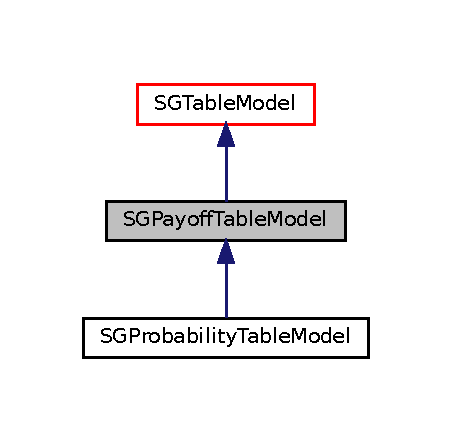
\includegraphics[width=217pt]{classSGPayoffTableModel__inherit__graph}
\end{center}
\end{figure}


Collaboration diagram for S\+G\+Payoff\+Table\+Model\+:
\nopagebreak
\begin{figure}[H]
\begin{center}
\leavevmode
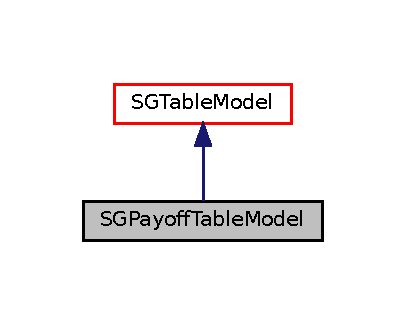
\includegraphics[width=195pt]{classSGPayoffTableModel__coll__graph}
\end{center}
\end{figure}
\subsection*{Public Member Functions}
\begin{DoxyCompactItemize}
\item 
\mbox{\Hypertarget{classSGPayoffTableModel_ab6768d4b56d310752769d6b4eb094323}\label{classSGPayoffTableModel_ab6768d4b56d310752769d6b4eb094323}} 
\hyperlink{classSGPayoffTableModel_ab6768d4b56d310752769d6b4eb094323}{S\+G\+Payoff\+Table\+Model} (\hyperlink{classSGGame}{S\+G\+Game} $\ast$\+\_\+game, int \+\_\+state)
\begin{DoxyCompactList}\small\item\em Constructor. \end{DoxyCompactList}\item 
Q\+Variant \hyperlink{classSGPayoffTableModel_ad47a81403a6442bd2fb879b52beea8c1}{data} (const Q\+Model\+Index \&index, int role) const Q\+\_\+\+D\+E\+C\+L\+\_\+\+O\+V\+E\+R\+R\+I\+DE
\begin{DoxyCompactList}\small\item\em Returns formatted data. \end{DoxyCompactList}\item 
Q\+Variant \hyperlink{classSGPayoffTableModel_a8473c095d2a00721bd36c196f2b90b95}{header\+Data} (int section, Qt\+::\+Orientation orientation, int role) const Q\+\_\+\+D\+E\+C\+L\+\_\+\+O\+V\+E\+R\+R\+I\+DE
\begin{DoxyCompactList}\small\item\em Returns formatted header data. \end{DoxyCompactList}\item 
bool \hyperlink{classSGPayoffTableModel_a9be799422c8a564a00911e959c795b5d}{set\+Data} (const Q\+Model\+Index \&index, const Q\+Variant \&value, int role)
\begin{DoxyCompactList}\small\item\em Sets data. \end{DoxyCompactList}\end{DoxyCompactItemize}
\subsection*{Additional Inherited Members}


\subsection{Detailed Description}
Derived class for payoff table models. 

This class handles the interface between \hyperlink{classSGTableView}{S\+G\+Table\+View} and the payoff matrices in \hyperlink{classSGGameHandler_ac95a8d363c98979cbbd8fc63a112bf11}{S\+G\+Game\+Handler\+::game}. Adds functionality for header data (using the row player action/ column player action conventions. Also reimplements the \hyperlink{classSGPayoffTableModel_ad47a81403a6442bd2fb879b52beea8c1}{data()} method to display an ordered pair of the two players\textquotesingle{} payoffs. 

\subsection{Member Function Documentation}
\mbox{\Hypertarget{classSGPayoffTableModel_ad47a81403a6442bd2fb879b52beea8c1}\label{classSGPayoffTableModel_ad47a81403a6442bd2fb879b52beea8c1}} 
\index{S\+G\+Payoff\+Table\+Model@{S\+G\+Payoff\+Table\+Model}!data@{data}}
\index{data@{data}!S\+G\+Payoff\+Table\+Model@{S\+G\+Payoff\+Table\+Model}}
\subsubsection{\texorpdfstring{data()}{data()}}
{\footnotesize\ttfamily Q\+Variant S\+G\+Payoff\+Table\+Model\+::data (\begin{DoxyParamCaption}\item[{const Q\+Model\+Index \&}]{index,  }\item[{int}]{role }\end{DoxyParamCaption}) const}



Returns formatted data. 

Returns an ordered pair of the two players\textquotesingle{} payoffs for the action profile specified in index. Reads this data from the game object using \hyperlink{classSGGame_a37036f4f8389a68c53b12eb75c1eb7af}{S\+G\+Game\+::get\+Payoffs}. \mbox{\Hypertarget{classSGPayoffTableModel_a8473c095d2a00721bd36c196f2b90b95}\label{classSGPayoffTableModel_a8473c095d2a00721bd36c196f2b90b95}} 
\index{S\+G\+Payoff\+Table\+Model@{S\+G\+Payoff\+Table\+Model}!header\+Data@{header\+Data}}
\index{header\+Data@{header\+Data}!S\+G\+Payoff\+Table\+Model@{S\+G\+Payoff\+Table\+Model}}
\subsubsection{\texorpdfstring{header\+Data()}{headerData()}}
{\footnotesize\ttfamily Q\+Variant S\+G\+Payoff\+Table\+Model\+::header\+Data (\begin{DoxyParamCaption}\item[{int}]{section,  }\item[{Qt\+::\+Orientation}]{orientation,  }\item[{int}]{role }\end{DoxyParamCaption}) const}



Returns formatted header data. 

Returns header data formatted to indicate the appropriate row/ column action. \mbox{\Hypertarget{classSGPayoffTableModel_a9be799422c8a564a00911e959c795b5d}\label{classSGPayoffTableModel_a9be799422c8a564a00911e959c795b5d}} 
\index{S\+G\+Payoff\+Table\+Model@{S\+G\+Payoff\+Table\+Model}!set\+Data@{set\+Data}}
\index{set\+Data@{set\+Data}!S\+G\+Payoff\+Table\+Model@{S\+G\+Payoff\+Table\+Model}}
\subsubsection{\texorpdfstring{set\+Data()}{setData()}}
{\footnotesize\ttfamily bool S\+G\+Payoff\+Table\+Model\+::set\+Data (\begin{DoxyParamCaption}\item[{const Q\+Model\+Index \&}]{index,  }\item[{const Q\+Variant \&}]{value,  }\item[{int}]{role }\end{DoxyParamCaption})}



Sets data. 

Parses the data in value to set a new pair of payoffs. Sets the data using S\+G\+Game\+::set\+Data. 

The documentation for this class was generated from the following files\+:\begin{DoxyCompactItemize}
\item 
viewer/hpp/sgpayofftablemodel.\+hpp\item 
viewer/cpp/sgpayofftablemodel.\+cpp\end{DoxyCompactItemize}

\hypertarget{classSGPlotController}{}\section{S\+G\+Plot\+Controller Class Reference}
\label{classSGPlotController}\index{S\+G\+Plot\+Controller@{S\+G\+Plot\+Controller}}


Handles the plot settings for \hyperlink{classSGSolutionHandler}{S\+G\+Solution\+Handler}.  




{\ttfamily \#include $<$sgplotcontroller.\+hpp$>$}



Inheritance diagram for S\+G\+Plot\+Controller\+:
\nopagebreak
\begin{figure}[H]
\begin{center}
\leavevmode
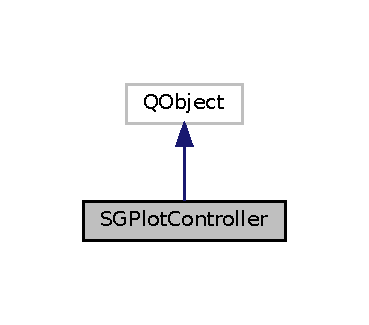
\includegraphics[width=177pt]{classSGPlotController__inherit__graph}
\end{center}
\end{figure}


Collaboration diagram for S\+G\+Plot\+Controller\+:
\nopagebreak
\begin{figure}[H]
\begin{center}
\leavevmode
\includegraphics[width=333pt]{classSGPlotController__coll__graph}
\end{center}
\end{figure}
\subsection*{Public Types}
\begin{DoxyCompactItemize}
\item 
enum \hyperlink{classSGPlotController_a04993344b70e1ac27322f54e43f5bce1}{Plot\+Mode} \{ \hyperlink{classSGPlotController_a04993344b70e1ac27322f54e43f5bce1aaace992b25a6ae65d522747ea10690c7}{Directions}, 
\hyperlink{classSGPlotController_a04993344b70e1ac27322f54e43f5bce1af4b6cf87b680d5b00b0939d0d9744043}{Generation}
 \}\begin{DoxyCompactList}\small\item\em Plot mode for the detail\+Plot. \end{DoxyCompactList}
\item 
enum \hyperlink{classSGPlotController_a7b1cebc57af82edfcbd1d2841ffad95c}{Solution\+Mode} \{ \hyperlink{classSGPlotController_a7b1cebc57af82edfcbd1d2841ffad95cac93156b79a026d54b4b692977da89e87}{Progress}, 
\hyperlink{classSGPlotController_a7b1cebc57af82edfcbd1d2841ffad95ca20f484d13a178c3ac5e886b798efa791}{Final}
 \}\begin{DoxyCompactList}\small\item\em Solution mode. \end{DoxyCompactList}
\end{DoxyCompactItemize}
\subsection*{Public Slots}
\begin{DoxyCompactItemize}
\item 
\mbox{\Hypertarget{classSGPlotController_aded7c120acb427ad77d4e57ce79f4e0d}\label{classSGPlotController_aded7c120acb427ad77d4e57ce79f4e0d}} 
void \hyperlink{classSGPlotController_aded7c120acb427ad77d4e57ce79f4e0d}{change\+Mode} (int new\+Mode)
\begin{DoxyCompactList}\small\item\em Toggles the solution mode. \end{DoxyCompactList}\item 
\mbox{\Hypertarget{classSGPlotController_ae34ccf38225310038155d3f815e98793}\label{classSGPlotController_ae34ccf38225310038155d3f815e98793}} 
void \hyperlink{classSGPlotController_ae34ccf38225310038155d3f815e98793}{iter\+Slider\+Update} (int value)
\begin{DoxyCompactList}\small\item\em Slot when the iter and start sliders are moved. \end{DoxyCompactList}\item 
void \hyperlink{classSGPlotController_a30efaeb2ec5cb752d6354f05447b287a}{set\+Slider\+Ranges} (int start, int end)
\item 
\mbox{\Hypertarget{classSGPlotController_a353dbab68b537e6443e7141a3e20f383}\label{classSGPlotController_a353dbab68b537e6443e7141a3e20f383}} 
void \hyperlink{classSGPlotController_a353dbab68b537e6443e7141a3e20f383}{prev\+Action} ()
\begin{DoxyCompactList}\small\item\em Decrements the action. \end{DoxyCompactList}\item 
\mbox{\Hypertarget{classSGPlotController_a3ccda5aca5a19194fb5699e62a6307d5}\label{classSGPlotController_a3ccda5aca5a19194fb5699e62a6307d5}} 
void \hyperlink{classSGPlotController_a3ccda5aca5a19194fb5699e62a6307d5}{next\+Action} ()
\begin{DoxyCompactList}\small\item\em Increments the action. \end{DoxyCompactList}\item 
\mbox{\Hypertarget{classSGPlotController_a4aab087b3ee5e3da82652510bba54048}\label{classSGPlotController_a4aab087b3ee5e3da82652510bba54048}} 
void \hyperlink{classSGPlotController_a4aab087b3ee5e3da82652510bba54048}{change\+Action} (int new\+Action)
\begin{DoxyCompactList}\small\item\em Sets the action. \end{DoxyCompactList}\end{DoxyCompactItemize}
\subsection*{Signals}
\begin{DoxyCompactItemize}
\item 
\mbox{\Hypertarget{classSGPlotController_a8f7d30a1e5aaf22cd7e891f6a70518eb}\label{classSGPlotController_a8f7d30a1e5aaf22cd7e891f6a70518eb}} 
void \hyperlink{classSGPlotController_a8f7d30a1e5aaf22cd7e891f6a70518eb}{solution\+Changed} ()
\begin{DoxyCompactList}\small\item\em Signal to the state and action models that the solution changed. \end{DoxyCompactList}\item 
\mbox{\Hypertarget{classSGPlotController_a5dae7775721c060e8d953a7f86e4aedf}\label{classSGPlotController_a5dae7775721c060e8d953a7f86e4aedf}} 
void \hyperlink{classSGPlotController_a5dae7775721c060e8d953a7f86e4aedf}{action\+Changed} ()
\begin{DoxyCompactList}\small\item\em Signal to the solution\+Handler that the action changed. \end{DoxyCompactList}\item 
\mbox{\Hypertarget{classSGPlotController_ae24292f1d18e5eb5debb56e4e186c953}\label{classSGPlotController_ae24292f1d18e5eb5debb56e4e186c953}} 
void \hyperlink{classSGPlotController_ae24292f1d18e5eb5debb56e4e186c953}{iteration\+Changed} ()
\begin{DoxyCompactList}\small\item\em Signal to solution\+Handler that the iteration changed. \end{DoxyCompactList}\end{DoxyCompactItemize}
\subsection*{Public Member Functions}
\begin{DoxyCompactItemize}
\item 
\mbox{\Hypertarget{classSGPlotController_ac69ac7f2655141d6ed05b30216066885}\label{classSGPlotController_ac69ac7f2655141d6ed05b30216066885}} 
\hyperlink{classSGPlotController_ac69ac7f2655141d6ed05b30216066885}{S\+G\+Plot\+Controller} (Q\+Combo\+Box $\ast$\+\_\+state\+Combo, Q\+Combo\+Box $\ast$\+\_\+action\+Combo, Q\+Scroll\+Bar $\ast$\+\_\+iter\+Slider, Q\+Scroll\+Bar $\ast$\+\_\+start\+Slider, Q\+Combo\+Box $\ast$\+\_\+solution\+Mode\+Combo)
\begin{DoxyCompactList}\small\item\em Constructor. \end{DoxyCompactList}\item 
\mbox{\Hypertarget{classSGPlotController_af4d02a19c7a3a29959f2c7e02826831e}\label{classSGPlotController_af4d02a19c7a3a29959f2c7e02826831e}} 
int \hyperlink{classSGPlotController_af4d02a19c7a3a29959f2c7e02826831e}{get\+State} () const
\begin{DoxyCompactList}\small\item\em Access method for the current state. \end{DoxyCompactList}\item 
\mbox{\Hypertarget{classSGPlotController_ab80599d82f9d4823c376c52f845e7f6e}\label{classSGPlotController_ab80599d82f9d4823c376c52f845e7f6e}} 
int \hyperlink{classSGPlotController_ab80599d82f9d4823c376c52f845e7f6e}{get\+Action} () const
\begin{DoxyCompactList}\small\item\em Access method for the current action. \end{DoxyCompactList}\item 
\mbox{\Hypertarget{classSGPlotController_a7981d2ad2ce8c37a0acf8d0855a309c8}\label{classSGPlotController_a7981d2ad2ce8c37a0acf8d0855a309c8}} 
int \hyperlink{classSGPlotController_a7981d2ad2ce8c37a0acf8d0855a309c8}{get\+Action\+Index} () const
\begin{DoxyCompactList}\small\item\em Access method for the current action index. \end{DoxyCompactList}\item 
\mbox{\Hypertarget{classSGPlotController_a3feedf398c637ccc61da156098c97f5c}\label{classSGPlotController_a3feedf398c637ccc61da156098c97f5c}} 
int \hyperlink{classSGPlotController_a3feedf398c637ccc61da156098c97f5c}{get\+Iteration} () const
\begin{DoxyCompactList}\small\item\em Access method for the current iteration number. \end{DoxyCompactList}\item 
\mbox{\Hypertarget{classSGPlotController_a7e98684c6af2fd4c6502cf528c8e4dc5}\label{classSGPlotController_a7e98684c6af2fd4c6502cf528c8e4dc5}} 
\hyperlink{classSGPlotController_a04993344b70e1ac27322f54e43f5bce1}{Plot\+Mode} \hyperlink{classSGPlotController_a7e98684c6af2fd4c6502cf528c8e4dc5}{get\+Plot\+Mode} () const
\begin{DoxyCompactList}\small\item\em Access method for the current plot mode. \end{DoxyCompactList}\item 
\mbox{\Hypertarget{classSGPlotController_a7dcba17b7cb912f96da1965a669127fe}\label{classSGPlotController_a7dcba17b7cb912f96da1965a669127fe}} 
\hyperlink{classSGPlotController_a7b1cebc57af82edfcbd1d2841ffad95c}{Solution\+Mode} \hyperlink{classSGPlotController_a7dcba17b7cb912f96da1965a669127fe}{get\+Mode} () const
\begin{DoxyCompactList}\small\item\em Access method for the current solution mode. \end{DoxyCompactList}\item 
\mbox{\Hypertarget{classSGPlotController_a857f9b6260f024bad00e68a5cc0e8edd}\label{classSGPlotController_a857f9b6260f024bad00e68a5cc0e8edd}} 
const \hyperlink{classSGIteration}{S\+G\+Iteration} \& \hyperlink{classSGPlotController_a857f9b6260f024bad00e68a5cc0e8edd}{get\+Current\+Iter} () const
\begin{DoxyCompactList}\small\item\em Access method for the current \hyperlink{classSGIteration}{S\+G\+Iteration} pointer. \end{DoxyCompactList}\item 
\mbox{\Hypertarget{classSGPlotController_a47600a28556e4701cc94d0c5e54a438f}\label{classSGPlotController_a47600a28556e4701cc94d0c5e54a438f}} 
const \hyperlink{classSGIteration}{S\+G\+Iteration} \& \hyperlink{classSGPlotController_a47600a28556e4701cc94d0c5e54a438f}{get\+Start\+Iter} () const
\begin{DoxyCompactList}\small\item\em Access method for the start \hyperlink{classSGIteration}{S\+G\+Iteration} pointer. \end{DoxyCompactList}\item 
\mbox{\Hypertarget{classSGPlotController_ab58cbd98d25e98ecd905b9c2ba2c2c6b}\label{classSGPlotController_ab58cbd98d25e98ecd905b9c2ba2c2c6b}} 
const \hyperlink{classSGIteration}{S\+G\+Iteration} \& \hyperlink{classSGPlotController_ab58cbd98d25e98ecd905b9c2ba2c2c6b}{get\+End\+Iter} () const
\begin{DoxyCompactList}\small\item\em Access method for the end \hyperlink{classSGIteration}{S\+G\+Iteration} pointer. \end{DoxyCompactList}\item 
\mbox{\Hypertarget{classSGPlotController_ae00c2c6453213013a890f0723ef3e168}\label{classSGPlotController_ae00c2c6453213013a890f0723ef3e168}} 
const \hyperlink{classSGIteration}{S\+G\+Iteration} \& \hyperlink{classSGPlotController_ae00c2c6453213013a890f0723ef3e168}{get\+Start\+Of\+Last\+Rev} () const
\begin{DoxyCompactList}\small\item\em Access method for the \hyperlink{classSGIteration}{S\+G\+Iteration} pointer that starts the last revolution. \end{DoxyCompactList}\item 
\mbox{\Hypertarget{classSGPlotController_aaf368cb6f7e3893fa165c40ef3b17f50}\label{classSGPlotController_aaf368cb6f7e3893fa165c40ef3b17f50}} 
int \hyperlink{classSGPlotController_aaf368cb6f7e3893fa165c40ef3b17f50}{get\+Start\+Slider\+Position} () const
\begin{DoxyCompactList}\small\item\em Returns the position of the start\+Slider. \end{DoxyCompactList}\item 
\mbox{\Hypertarget{classSGPlotController_a21e04610454ab6936d782931d5fd35c5}\label{classSGPlotController_a21e04610454ab6936d782931d5fd35c5}} 
bool \hyperlink{classSGPlotController_a21e04610454ab6936d782931d5fd35c5}{has\+Solution} () const
\begin{DoxyCompactList}\small\item\em Returns true if a solution has been loaded. \end{DoxyCompactList}\item 
\mbox{\Hypertarget{classSGPlotController_ab6da5d8489ad707cf6d6c460517f303f}\label{classSGPlotController_ab6da5d8489ad707cf6d6c460517f303f}} 
const \hyperlink{classSGSolution}{S\+G\+Solution} $\ast$ \hyperlink{classSGPlotController_ab6da5d8489ad707cf6d6c460517f303f}{get\+Solution} () const
\begin{DoxyCompactList}\small\item\em Returns the current solution. \end{DoxyCompactList}\item 
\mbox{\Hypertarget{classSGPlotController_a1a2c3716912d030a1ed7259c62c402f1}\label{classSGPlotController_a1a2c3716912d030a1ed7259c62c402f1}} 
void \hyperlink{classSGPlotController_a1a2c3716912d030a1ed7259c62c402f1}{set\+Solution} (\hyperlink{classSGSolution}{S\+G\+Solution} $\ast$new\+Soln)
\begin{DoxyCompactList}\small\item\em Sets the solution. \end{DoxyCompactList}\item 
\mbox{\Hypertarget{classSGPlotController_a5026032dbc00ff3aa4abd05ea6401755}\label{classSGPlotController_a5026032dbc00ff3aa4abd05ea6401755}} 
bool \hyperlink{classSGPlotController_a5026032dbc00ff3aa4abd05ea6401755}{set\+State} (int new\+State)
\begin{DoxyCompactList}\small\item\em Sets the current state. \end{DoxyCompactList}\item 
\mbox{\Hypertarget{classSGPlotController_a4608e92513c0c0b1a75c682625567900}\label{classSGPlotController_a4608e92513c0c0b1a75c682625567900}} 
void \hyperlink{classSGPlotController_a4608e92513c0c0b1a75c682625567900}{set\+Plot\+Mode} (\hyperlink{classSGPlotController_a04993344b70e1ac27322f54e43f5bce1}{Plot\+Mode} new\+Mode)
\begin{DoxyCompactList}\small\item\em Sets the plot mode. \end{DoxyCompactList}\item 
\mbox{\Hypertarget{classSGPlotController_af6873a0f903bce322494c24dcec765d0}\label{classSGPlotController_af6873a0f903bce322494c24dcec765d0}} 
bool \hyperlink{classSGPlotController_af6873a0f903bce322494c24dcec765d0}{set\+Action\+Index} (int new\+Action\+Index)
\begin{DoxyCompactList}\small\item\em Sets the current action index. \end{DoxyCompactList}\item 
\mbox{\Hypertarget{classSGPlotController_ac08b1b71fea0d7b96a947a71c402ccae}\label{classSGPlotController_ac08b1b71fea0d7b96a947a71c402ccae}} 
bool \hyperlink{classSGPlotController_ac08b1b71fea0d7b96a947a71c402ccae}{set\+Action} (int new\+Action)
\begin{DoxyCompactList}\small\item\em Sets the current action. \end{DoxyCompactList}\item 
\mbox{\Hypertarget{classSGPlotController_aa77fca25b62a8206d3ddc1fa7cd16eac}\label{classSGPlotController_aa77fca25b62a8206d3ddc1fa7cd16eac}} 
bool \hyperlink{classSGPlotController_aa77fca25b62a8206d3ddc1fa7cd16eac}{set\+Iteration} (int new\+Iter)
\begin{DoxyCompactList}\small\item\em Sets the current iteration. \end{DoxyCompactList}\item 
\mbox{\Hypertarget{classSGPlotController_a45da9096f5457484fb8bc5c63c8b7fc5}\label{classSGPlotController_a45da9096f5457484fb8bc5c63c8b7fc5}} 
void \hyperlink{classSGPlotController_a45da9096f5457484fb8bc5c63c8b7fc5}{move\+Forwards} ()
\begin{DoxyCompactList}\small\item\em Increments the current iteration. \end{DoxyCompactList}\item 
\mbox{\Hypertarget{classSGPlotController_a918ec5fac2839b4a328289962e0ac441}\label{classSGPlotController_a918ec5fac2839b4a328289962e0ac441}} 
void \hyperlink{classSGPlotController_a918ec5fac2839b4a328289962e0ac441}{move\+Backwards} ()
\begin{DoxyCompactList}\small\item\em Decrements the current iteration. \end{DoxyCompactList}\item 
void \hyperlink{classSGPlotController_a3b0857d4b4c40bbac853ded334573fa0}{set\+Current\+Iteration} (\hyperlink{classSGPoint}{S\+G\+Point} point, int \hyperlink{classSGPlotController_aaef95a25f39e465b01cc92770d93bd2d}{state})
\item 
void \hyperlink{classSGPlotController_a2d4971bb9f2f6116ce314d146a43bb08}{synchronize\+Sliders} ()
\begin{DoxyCompactList}\small\item\em Synchronizes sliders with controls. \end{DoxyCompactList}\end{DoxyCompactItemize}
\subsection*{Private Attributes}
\begin{DoxyCompactItemize}
\item 
\mbox{\Hypertarget{classSGPlotController_aaef95a25f39e465b01cc92770d93bd2d}\label{classSGPlotController_aaef95a25f39e465b01cc92770d93bd2d}} 
int \hyperlink{classSGPlotController_aaef95a25f39e465b01cc92770d93bd2d}{state}
\begin{DoxyCompactList}\small\item\em Current state. \end{DoxyCompactList}\item 
\mbox{\Hypertarget{classSGPlotController_ab7e15498eb6bc5e88deafb2eb1ecaa33}\label{classSGPlotController_ab7e15498eb6bc5e88deafb2eb1ecaa33}} 
int \hyperlink{classSGPlotController_ab7e15498eb6bc5e88deafb2eb1ecaa33}{action}
\begin{DoxyCompactList}\small\item\em Current action. \end{DoxyCompactList}\item 
int \hyperlink{classSGPlotController_a0baff45708bb3bf9fd976975cd0d6ac4}{action\+Index}
\item 
\mbox{\Hypertarget{classSGPlotController_ad6886fa2d62aec157332c07d8f91b145}\label{classSGPlotController_ad6886fa2d62aec157332c07d8f91b145}} 
int \hyperlink{classSGPlotController_ad6886fa2d62aec157332c07d8f91b145}{iteration}
\begin{DoxyCompactList}\small\item\em The current iteration. \end{DoxyCompactList}\item 
\mbox{\Hypertarget{classSGPlotController_abc03425a174aa18b8d8994bc60ad2aa1}\label{classSGPlotController_abc03425a174aa18b8d8994bc60ad2aa1}} 
\hyperlink{classSGSolution}{S\+G\+Solution} $\ast$ \hyperlink{classSGPlotController_abc03425a174aa18b8d8994bc60ad2aa1}{soln}
\begin{DoxyCompactList}\small\item\em The current solution object. \end{DoxyCompactList}\item 
\mbox{\Hypertarget{classSGPlotController_addb72091bb689c8942522b4c54a4d4cf}\label{classSGPlotController_addb72091bb689c8942522b4c54a4d4cf}} 
\hyperlink{classSGPlotController_a04993344b70e1ac27322f54e43f5bce1}{Plot\+Mode} \hyperlink{classSGPlotController_addb72091bb689c8942522b4c54a4d4cf}{plot\+Mode}
\begin{DoxyCompactList}\small\item\em The current plot mode. \end{DoxyCompactList}\item 
\mbox{\Hypertarget{classSGPlotController_a8fdf83cc3dcef50537e142e7f8905668}\label{classSGPlotController_a8fdf83cc3dcef50537e142e7f8905668}} 
\hyperlink{classSGPlotController_a7b1cebc57af82edfcbd1d2841ffad95c}{Solution\+Mode} \hyperlink{classSGPlotController_a8fdf83cc3dcef50537e142e7f8905668}{mode}
\begin{DoxyCompactList}\small\item\em The current solution mode. \end{DoxyCompactList}\item 
\mbox{\Hypertarget{classSGPlotController_ae8f9f11e6f060c818603935a3c71e6f9}\label{classSGPlotController_ae8f9f11e6f060c818603935a3c71e6f9}} 
list$<$ \hyperlink{classSGIteration}{S\+G\+Iteration} $>$\+::const\+\_\+iterator \hyperlink{classSGPlotController_ae8f9f11e6f060c818603935a3c71e6f9}{start\+Iter}
\begin{DoxyCompactList}\small\item\em Points to the first \hyperlink{classSGIteration}{S\+G\+Iteration} object from which to plot. \end{DoxyCompactList}\item 
\mbox{\Hypertarget{classSGPlotController_afbca0fc2e4ecd8dae64559697b78ef91}\label{classSGPlotController_afbca0fc2e4ecd8dae64559697b78ef91}} 
list$<$ \hyperlink{classSGIteration}{S\+G\+Iteration} $>$\+::const\+\_\+iterator \hyperlink{classSGPlotController_afbca0fc2e4ecd8dae64559697b78ef91}{end\+Iter}
\begin{DoxyCompactList}\small\item\em Points to the last \hyperlink{classSGIteration}{S\+G\+Iteration} object to which to plot. \end{DoxyCompactList}\item 
\mbox{\Hypertarget{classSGPlotController_a4a174717197d238b483488a72f11e1eb}\label{classSGPlotController_a4a174717197d238b483488a72f11e1eb}} 
list$<$ \hyperlink{classSGIteration}{S\+G\+Iteration} $>$\+::const\+\_\+iterator \hyperlink{classSGPlotController_a4a174717197d238b483488a72f11e1eb}{current\+Iter}
\begin{DoxyCompactList}\small\item\em Points to the current S\+Giteration. \end{DoxyCompactList}\item 
\mbox{\Hypertarget{classSGPlotController_aad63498d4578179dcf705070668d5480}\label{classSGPlotController_aad63498d4578179dcf705070668d5480}} 
list$<$ \hyperlink{classSGIteration}{S\+G\+Iteration} $>$\+::const\+\_\+iterator \hyperlink{classSGPlotController_aad63498d4578179dcf705070668d5480}{start\+Of\+Last\+Rev}
\begin{DoxyCompactList}\small\item\em Points to the \hyperlink{classSGIteration}{S\+G\+Iteration} that starts the last revolution. \end{DoxyCompactList}\item 
\mbox{\Hypertarget{classSGPlotController_a6123551bcba7707373c316617e21b70e}\label{classSGPlotController_a6123551bcba7707373c316617e21b70e}} 
bool \hyperlink{classSGPlotController_a6123551bcba7707373c316617e21b70e}{soln\+Loaded}
\begin{DoxyCompactList}\small\item\em Indicates when an \hyperlink{classSGSolution}{S\+G\+Solution} object has been loaded. \end{DoxyCompactList}\item 
\mbox{\Hypertarget{classSGPlotController_a63ba05fcb3f660bf9fdd5fb42a0df05b}\label{classSGPlotController_a63ba05fcb3f660bf9fdd5fb42a0df05b}} 
Q\+Combo\+Box $\ast$ \hyperlink{classSGPlotController_a63ba05fcb3f660bf9fdd5fb42a0df05b}{state\+Combo}
\begin{DoxyCompactList}\small\item\em Points to the state\+Combo Q\+Combo\+Box selector. \end{DoxyCompactList}\item 
\mbox{\Hypertarget{classSGPlotController_aa0963a19f195b384a33ba3e8d6993423}\label{classSGPlotController_aa0963a19f195b384a33ba3e8d6993423}} 
Q\+Combo\+Box $\ast$ \hyperlink{classSGPlotController_aa0963a19f195b384a33ba3e8d6993423}{action\+Combo}
\begin{DoxyCompactList}\small\item\em Points to the action\+Combo Q\+Combo\+Box selector. \end{DoxyCompactList}\item 
\mbox{\Hypertarget{classSGPlotController_abb1605bd670c9850af648c1a9f39f2a3}\label{classSGPlotController_abb1605bd670c9850af648c1a9f39f2a3}} 
Q\+Combo\+Box $\ast$ \hyperlink{classSGPlotController_abb1605bd670c9850af648c1a9f39f2a3}{solution\+Mode\+Combo}
\begin{DoxyCompactList}\small\item\em Points to the solution\+Mode Q\+Combo\+Box selector. \end{DoxyCompactList}\item 
\mbox{\Hypertarget{classSGPlotController_a063783e3acc1d60734baed900e58fb42}\label{classSGPlotController_a063783e3acc1d60734baed900e58fb42}} 
Q\+Scroll\+Bar $\ast$ \hyperlink{classSGPlotController_a063783e3acc1d60734baed900e58fb42}{iter\+Slider}
\begin{DoxyCompactList}\small\item\em Points to the iter\+Slider Q\+Scroll\+Bar for selecting the current iteration. \end{DoxyCompactList}\item 
Q\+Scroll\+Bar $\ast$ \hyperlink{classSGPlotController_a399d56ae9da6dac78110e9b70e842ffe}{start\+Slider}
\end{DoxyCompactItemize}


\subsection{Detailed Description}
Handles the plot settings for \hyperlink{classSGSolutionHandler}{S\+G\+Solution\+Handler}. 

This class intermediates between the controllers (iter\+Slider, state\+Combo, action\+Combo) and the plotting methods in the S\+G\+S\+Solution\+Handler (i.\+e., plot\+Solution(...)).

See also viewersolutionsec. 

\subsection{Member Enumeration Documentation}
\mbox{\Hypertarget{classSGPlotController_a04993344b70e1ac27322f54e43f5bce1}\label{classSGPlotController_a04993344b70e1ac27322f54e43f5bce1}} 
\index{S\+G\+Plot\+Controller@{S\+G\+Plot\+Controller}!Plot\+Mode@{Plot\+Mode}}
\index{Plot\+Mode@{Plot\+Mode}!S\+G\+Plot\+Controller@{S\+G\+Plot\+Controller}}
\subsubsection{\texorpdfstring{Plot\+Mode}{PlotMode}}
{\footnotesize\ttfamily enum \hyperlink{classSGPlotController_a04993344b70e1ac27322f54e43f5bce1}{S\+G\+Plot\+Controller\+::\+Plot\+Mode}}



Plot mode for the detail\+Plot. 

Indicates whether to plot all of the test directions (Directions) or just plot the way the current pivot is generated (Generation). \begin{DoxyEnumFields}{Enumerator}
\raisebox{\heightof{T}}[0pt][0pt]{\index{Directions@{Directions}!S\+G\+Plot\+Controller@{S\+G\+Plot\+Controller}}\index{S\+G\+Plot\+Controller@{S\+G\+Plot\+Controller}!Directions@{Directions}}}\mbox{\Hypertarget{classSGPlotController_a04993344b70e1ac27322f54e43f5bce1aaace992b25a6ae65d522747ea10690c7}\label{classSGPlotController_a04993344b70e1ac27322f54e43f5bce1aaace992b25a6ae65d522747ea10690c7}} 
Directions&Plot the test directions. \\
\hline

\raisebox{\heightof{T}}[0pt][0pt]{\index{Generation@{Generation}!S\+G\+Plot\+Controller@{S\+G\+Plot\+Controller}}\index{S\+G\+Plot\+Controller@{S\+G\+Plot\+Controller}!Generation@{Generation}}}\mbox{\Hypertarget{classSGPlotController_a04993344b70e1ac27322f54e43f5bce1af4b6cf87b680d5b00b0939d0d9744043}\label{classSGPlotController_a04993344b70e1ac27322f54e43f5bce1af4b6cf87b680d5b00b0939d0d9744043}} 
Generation&Plot how the payoffs are generated. \\
\hline

\end{DoxyEnumFields}
\mbox{\Hypertarget{classSGPlotController_a7b1cebc57af82edfcbd1d2841ffad95c}\label{classSGPlotController_a7b1cebc57af82edfcbd1d2841ffad95c}} 
\index{S\+G\+Plot\+Controller@{S\+G\+Plot\+Controller}!Solution\+Mode@{Solution\+Mode}}
\index{Solution\+Mode@{Solution\+Mode}!S\+G\+Plot\+Controller@{S\+G\+Plot\+Controller}}
\subsubsection{\texorpdfstring{Solution\+Mode}{SolutionMode}}
{\footnotesize\ttfamily enum \hyperlink{classSGPlotController_a7b1cebc57af82edfcbd1d2841ffad95c}{S\+G\+Plot\+Controller\+::\+Solution\+Mode}}



Solution mode. 

Indicates whether or not to plot all of the iterations from a user-\/defined start point to the current iteration (Progress) or just plot all of the iterations on the last revolution (Final). \begin{DoxyEnumFields}{Enumerator}
\raisebox{\heightof{T}}[0pt][0pt]{\index{Progress@{Progress}!S\+G\+Plot\+Controller@{S\+G\+Plot\+Controller}}\index{S\+G\+Plot\+Controller@{S\+G\+Plot\+Controller}!Progress@{Progress}}}\mbox{\Hypertarget{classSGPlotController_a7b1cebc57af82edfcbd1d2841ffad95cac93156b79a026d54b4b692977da89e87}\label{classSGPlotController_a7b1cebc57af82edfcbd1d2841ffad95cac93156b79a026d54b4b692977da89e87}} 
Progress&Plot the progress of the algorithm. \\
\hline

\raisebox{\heightof{T}}[0pt][0pt]{\index{Final@{Final}!S\+G\+Plot\+Controller@{S\+G\+Plot\+Controller}}\index{S\+G\+Plot\+Controller@{S\+G\+Plot\+Controller}!Final@{Final}}}\mbox{\Hypertarget{classSGPlotController_a7b1cebc57af82edfcbd1d2841ffad95ca20f484d13a178c3ac5e886b798efa791}\label{classSGPlotController_a7b1cebc57af82edfcbd1d2841ffad95ca20f484d13a178c3ac5e886b798efa791}} 
Final&Plot the last revolution (the true correspondence) \\
\hline

\end{DoxyEnumFields}


\subsection{Member Function Documentation}
\mbox{\Hypertarget{classSGPlotController_a3b0857d4b4c40bbac853ded334573fa0}\label{classSGPlotController_a3b0857d4b4c40bbac853ded334573fa0}} 
\index{S\+G\+Plot\+Controller@{S\+G\+Plot\+Controller}!set\+Current\+Iteration@{set\+Current\+Iteration}}
\index{set\+Current\+Iteration@{set\+Current\+Iteration}!S\+G\+Plot\+Controller@{S\+G\+Plot\+Controller}}
\subsubsection{\texorpdfstring{set\+Current\+Iteration()}{setCurrentIteration()}}
{\footnotesize\ttfamily void S\+G\+Plot\+Controller\+::set\+Current\+Iteration (\begin{DoxyParamCaption}\item[{\hyperlink{classSGPoint}{S\+G\+Point}}]{point,  }\item[{int}]{state }\end{DoxyParamCaption})}

Sets the current iteration to be the one where the pivot in the given state is closest to point. \mbox{\Hypertarget{classSGPlotController_a30efaeb2ec5cb752d6354f05447b287a}\label{classSGPlotController_a30efaeb2ec5cb752d6354f05447b287a}} 
\index{S\+G\+Plot\+Controller@{S\+G\+Plot\+Controller}!set\+Slider\+Ranges@{set\+Slider\+Ranges}}
\index{set\+Slider\+Ranges@{set\+Slider\+Ranges}!S\+G\+Plot\+Controller@{S\+G\+Plot\+Controller}}
\subsubsection{\texorpdfstring{set\+Slider\+Ranges}{setSliderRanges}}
{\footnotesize\ttfamily void S\+G\+Plot\+Controller\+::set\+Slider\+Ranges (\begin{DoxyParamCaption}\item[{int}]{start,  }\item[{int}]{end }\end{DoxyParamCaption})\hspace{0.3cm}{\ttfamily [slot]}}

Slot used to set up the sliders when changing between Progress and Final modes. \mbox{\Hypertarget{classSGPlotController_a2d4971bb9f2f6116ce314d146a43bb08}\label{classSGPlotController_a2d4971bb9f2f6116ce314d146a43bb08}} 
\index{S\+G\+Plot\+Controller@{S\+G\+Plot\+Controller}!synchronize\+Sliders@{synchronize\+Sliders}}
\index{synchronize\+Sliders@{synchronize\+Sliders}!S\+G\+Plot\+Controller@{S\+G\+Plot\+Controller}}
\subsubsection{\texorpdfstring{synchronize\+Sliders()}{synchronizeSliders()}}
{\footnotesize\ttfamily void S\+G\+Plot\+Controller\+::synchronize\+Sliders (\begin{DoxyParamCaption}{ }\end{DoxyParamCaption})}



Synchronizes sliders with controls. 

Sets start\+Iter and current\+Iter to be equal to the values indicated in the respective sliders. 

\subsection{Member Data Documentation}
\mbox{\Hypertarget{classSGPlotController_a0baff45708bb3bf9fd976975cd0d6ac4}\label{classSGPlotController_a0baff45708bb3bf9fd976975cd0d6ac4}} 
\index{S\+G\+Plot\+Controller@{S\+G\+Plot\+Controller}!action\+Index@{action\+Index}}
\index{action\+Index@{action\+Index}!S\+G\+Plot\+Controller@{S\+G\+Plot\+Controller}}
\subsubsection{\texorpdfstring{action\+Index}{actionIndex}}
{\footnotesize\ttfamily int S\+G\+Plot\+Controller\+::action\+Index\hspace{0.3cm}{\ttfamily [private]}}

Index of the current action within the list of actions in current\+Iter-\/$>$actions\mbox{[}state\mbox{]} \mbox{\Hypertarget{classSGPlotController_a399d56ae9da6dac78110e9b70e842ffe}\label{classSGPlotController_a399d56ae9da6dac78110e9b70e842ffe}} 
\index{S\+G\+Plot\+Controller@{S\+G\+Plot\+Controller}!start\+Slider@{start\+Slider}}
\index{start\+Slider@{start\+Slider}!S\+G\+Plot\+Controller@{S\+G\+Plot\+Controller}}
\subsubsection{\texorpdfstring{start\+Slider}{startSlider}}
{\footnotesize\ttfamily Q\+Scroll\+Bar$\ast$ S\+G\+Plot\+Controller\+::start\+Slider\hspace{0.3cm}{\ttfamily [private]}}

Points to the start\+Slider Q\+Scroll\+Bar for selecting the start iteration when the solution mode is Progress. 

The documentation for this class was generated from the following files\+:\begin{DoxyCompactItemize}
\item 
viewer/hpp/sgplotcontroller.\+hpp\item 
viewer/cpp/sgplotcontroller.\+cpp\end{DoxyCompactItemize}

\hypertarget{classSGPlotController__V2}{}\section{S\+G\+Plot\+Controller\+\_\+\+V2 Class Reference}
\label{classSGPlotController__V2}\index{S\+G\+Plot\+Controller\+\_\+\+V2@{S\+G\+Plot\+Controller\+\_\+\+V2}}


Handles the plot settings for \hyperlink{classSGSolutionHandler}{S\+G\+Solution\+Handler}.  




{\ttfamily \#include $<$sgplotcontroller\+\_\+v2.\+hpp$>$}



Inheritance diagram for S\+G\+Plot\+Controller\+\_\+\+V2\+:
\nopagebreak
\begin{figure}[H]
\begin{center}
\leavevmode
\includegraphics[width=195pt]{classSGPlotController__V2__inherit__graph}
\end{center}
\end{figure}


Collaboration diagram for S\+G\+Plot\+Controller\+\_\+\+V2\+:
\nopagebreak
\begin{figure}[H]
\begin{center}
\leavevmode
\includegraphics[width=350pt]{classSGPlotController__V2__coll__graph}
\end{center}
\end{figure}
\subsection*{Public Types}
\begin{DoxyCompactItemize}
\item 
enum \hyperlink{classSGPlotController__V2_a406df03a36c19d6e12ba340b3abddb34}{Plot\+Mode} \{ \hyperlink{classSGPlotController__V2_a406df03a36c19d6e12ba340b3abddb34a9b299f65421319463ca259ab6a36ff04}{Directions}, 
\hyperlink{classSGPlotController__V2_a406df03a36c19d6e12ba340b3abddb34ab51f8aefb68c79196507bd594e31a5d6}{Generation}
 \}\begin{DoxyCompactList}\small\item\em Plot mode for the detail\+Plot. \end{DoxyCompactList}
\item 
enum \hyperlink{classSGPlotController__V2_a1a1b0d79a2202a7a5c7dd24ac8885677}{Solution\+Mode} \{ \hyperlink{classSGPlotController__V2_a1a1b0d79a2202a7a5c7dd24ac8885677af9627cbf5cd18f82785e0cfed31237e0}{Progress}, 
\hyperlink{classSGPlotController__V2_a1a1b0d79a2202a7a5c7dd24ac8885677a5f2f2e1e7b99bd5d4117b80ca0fb2e01}{Final}
 \}\begin{DoxyCompactList}\small\item\em Solution mode. \end{DoxyCompactList}
\end{DoxyCompactItemize}
\subsection*{Public Slots}
\begin{DoxyCompactItemize}
\item 
\mbox{\Hypertarget{classSGPlotController__V2_a2d224cc2f5c0f0d405fb761710332ff0}\label{classSGPlotController__V2_a2d224cc2f5c0f0d405fb761710332ff0}} 
void \hyperlink{classSGPlotController__V2_a2d224cc2f5c0f0d405fb761710332ff0}{iter\+Slider\+Update} (int value)
\begin{DoxyCompactList}\small\item\em Slot when the iter and start sliders are moved. \end{DoxyCompactList}\item 
\mbox{\Hypertarget{classSGPlotController__V2_ade8b50f8578a22e8d84a8ed959c1d692}\label{classSGPlotController__V2_ade8b50f8578a22e8d84a8ed959c1d692}} 
void \hyperlink{classSGPlotController__V2_ade8b50f8578a22e8d84a8ed959c1d692}{prev\+Action} ()
\begin{DoxyCompactList}\small\item\em Decrements the action. \end{DoxyCompactList}\item 
\mbox{\Hypertarget{classSGPlotController__V2_a780e6182f5ac8581e3551355c22d1678}\label{classSGPlotController__V2_a780e6182f5ac8581e3551355c22d1678}} 
void \hyperlink{classSGPlotController__V2_a780e6182f5ac8581e3551355c22d1678}{next\+Action} ()
\begin{DoxyCompactList}\small\item\em Increments the action. \end{DoxyCompactList}\item 
\mbox{\Hypertarget{classSGPlotController__V2_aa22b2fa8f7fa99cd5a03554724184b96}\label{classSGPlotController__V2_aa22b2fa8f7fa99cd5a03554724184b96}} 
void \hyperlink{classSGPlotController__V2_aa22b2fa8f7fa99cd5a03554724184b96}{change\+Action} (int new\+Action)
\begin{DoxyCompactList}\small\item\em Sets the action. \end{DoxyCompactList}\item 
\mbox{\Hypertarget{classSGPlotController__V2_aad05b4160938117e293ee78daca77da7}\label{classSGPlotController__V2_aad05b4160938117e293ee78daca77da7}} 
void \hyperlink{classSGPlotController__V2_aad05b4160938117e293ee78daca77da7}{change\+Mode} (int new\+Mode)
\begin{DoxyCompactList}\small\item\em Toggles the solution mode. \end{DoxyCompactList}\end{DoxyCompactItemize}
\subsection*{Signals}
\begin{DoxyCompactItemize}
\item 
\mbox{\Hypertarget{classSGPlotController__V2_add52b2f05d4adff7f1d02faf3e6588fb}\label{classSGPlotController__V2_add52b2f05d4adff7f1d02faf3e6588fb}} 
void \hyperlink{classSGPlotController__V2_add52b2f05d4adff7f1d02faf3e6588fb}{solution\+Changed} ()
\begin{DoxyCompactList}\small\item\em Signal to the state and action models that the solution changed. \end{DoxyCompactList}\item 
\mbox{\Hypertarget{classSGPlotController__V2_a4a6d19fa34127439f4997f379abd9604}\label{classSGPlotController__V2_a4a6d19fa34127439f4997f379abd9604}} 
void \hyperlink{classSGPlotController__V2_a4a6d19fa34127439f4997f379abd9604}{action\+Changed} ()
\begin{DoxyCompactList}\small\item\em Signal to the solution\+Handler that the action changed. \end{DoxyCompactList}\item 
\mbox{\Hypertarget{classSGPlotController__V2_ad0b30bfba68303c2a4252de98ecb6d8e}\label{classSGPlotController__V2_ad0b30bfba68303c2a4252de98ecb6d8e}} 
void \hyperlink{classSGPlotController__V2_ad0b30bfba68303c2a4252de98ecb6d8e}{state\+Changed} ()
\begin{DoxyCompactList}\small\item\em Signal to the action\+Combo that the state changed. \end{DoxyCompactList}\item 
\mbox{\Hypertarget{classSGPlotController__V2_a1ab601bb4a50d7a15dbda5de0d577ca0}\label{classSGPlotController__V2_a1ab601bb4a50d7a15dbda5de0d577ca0}} 
void \hyperlink{classSGPlotController__V2_a1ab601bb4a50d7a15dbda5de0d577ca0}{iteration\+Changed} ()
\begin{DoxyCompactList}\small\item\em Signal to solution\+Handler that the iteration changed. \end{DoxyCompactList}\end{DoxyCompactItemize}
\subsection*{Public Member Functions}
\begin{DoxyCompactItemize}
\item 
\mbox{\Hypertarget{classSGPlotController__V2_ab1ed25aaf2dce288131242db73a38317}\label{classSGPlotController__V2_ab1ed25aaf2dce288131242db73a38317}} 
\hyperlink{classSGPlotController__V2_ab1ed25aaf2dce288131242db73a38317}{S\+G\+Plot\+Controller\+\_\+\+V2} (Q\+Combo\+Box $\ast$\+\_\+state\+Combo, Q\+Combo\+Box $\ast$\+\_\+action\+Combo, Q\+Scroll\+Bar $\ast$\+\_\+iter\+Slider, Q\+Scroll\+Bar $\ast$\+\_\+step\+Slider, Q\+Combo\+Box $\ast$\+\_\+solution\+Mode\+Combo)
\begin{DoxyCompactList}\small\item\em Constructor. \end{DoxyCompactList}\item 
\mbox{\Hypertarget{classSGPlotController__V2_ae372dd39da9f733a8a50f57a52a159bb}\label{classSGPlotController__V2_ae372dd39da9f733a8a50f57a52a159bb}} 
int \hyperlink{classSGPlotController__V2_ae372dd39da9f733a8a50f57a52a159bb}{get\+State} () const
\begin{DoxyCompactList}\small\item\em Access method for the current state. \end{DoxyCompactList}\item 
\mbox{\Hypertarget{classSGPlotController__V2_aaddfae6fda7755460fc1fec3f19307b0}\label{classSGPlotController__V2_aaddfae6fda7755460fc1fec3f19307b0}} 
int \hyperlink{classSGPlotController__V2_aaddfae6fda7755460fc1fec3f19307b0}{get\+Action} () const
\begin{DoxyCompactList}\small\item\em Access method for the current action. \end{DoxyCompactList}\item 
\mbox{\Hypertarget{classSGPlotController__V2_a3f447b7556a51274e7d96d6e7af2b8fb}\label{classSGPlotController__V2_a3f447b7556a51274e7d96d6e7af2b8fb}} 
int \hyperlink{classSGPlotController__V2_a3f447b7556a51274e7d96d6e7af2b8fb}{get\+Action\+Index} () const
\begin{DoxyCompactList}\small\item\em Access method for the current action index. \end{DoxyCompactList}\item 
\mbox{\Hypertarget{classSGPlotController__V2_ae5d3ea93a15ececf05c3fb9cceba9f57}\label{classSGPlotController__V2_ae5d3ea93a15ececf05c3fb9cceba9f57}} 
int \hyperlink{classSGPlotController__V2_ae5d3ea93a15ececf05c3fb9cceba9f57}{get\+Iteration} () const
\begin{DoxyCompactList}\small\item\em Access method for the current iteration number. \end{DoxyCompactList}\item 
\mbox{\Hypertarget{classSGPlotController__V2_acf16c0fb426ea62da139806175a9ca2d}\label{classSGPlotController__V2_acf16c0fb426ea62da139806175a9ca2d}} 
\hyperlink{classSGPlotController__V2_a406df03a36c19d6e12ba340b3abddb34}{Plot\+Mode} \hyperlink{classSGPlotController__V2_acf16c0fb426ea62da139806175a9ca2d}{get\+Plot\+Mode} () const
\begin{DoxyCompactList}\small\item\em Access method for the current plot mode. \end{DoxyCompactList}\item 
\mbox{\Hypertarget{classSGPlotController__V2_a63040af9509c211b35b3feaa73a48aba}\label{classSGPlotController__V2_a63040af9509c211b35b3feaa73a48aba}} 
\hyperlink{classSGPlotController__V2_a1a1b0d79a2202a7a5c7dd24ac8885677}{Solution\+Mode} \hyperlink{classSGPlotController__V2_a63040af9509c211b35b3feaa73a48aba}{get\+Mode} () const
\begin{DoxyCompactList}\small\item\em Access method for the current solution mode. \end{DoxyCompactList}\item 
\mbox{\Hypertarget{classSGPlotController__V2_aa7ba918a44f28a2cac0dae929dd70fff}\label{classSGPlotController__V2_aa7ba918a44f28a2cac0dae929dd70fff}} 
list$<$ \hyperlink{classSGIteration__MaxMinMax}{S\+G\+Iteration\+\_\+\+Max\+Min\+Max} $>$\+::const\+\_\+iterator \hyperlink{classSGPlotController__V2_aa7ba918a44f28a2cac0dae929dd70fff}{get\+Current\+Iter} () const
\begin{DoxyCompactList}\small\item\em Access method for the current \hyperlink{classSGIteration__MaxMinMax}{S\+G\+Iteration\+\_\+\+Max\+Min\+Max} pointer. \end{DoxyCompactList}\item 
\mbox{\Hypertarget{classSGPlotController__V2_ae31ded80aeff97dc2e130778433ec4e7}\label{classSGPlotController__V2_ae31ded80aeff97dc2e130778433ec4e7}} 
int \hyperlink{classSGPlotController__V2_ae31ded80aeff97dc2e130778433ec4e7}{get\+Current\+Iter\+Index} () const
\begin{DoxyCompactList}\small\item\em Access method for the current \hyperlink{classSGIteration__MaxMinMax}{S\+G\+Iteration\+\_\+\+Max\+Min\+Max} pointer. \end{DoxyCompactList}\item 
\mbox{\Hypertarget{classSGPlotController__V2_a837430ca072623f8a84aa94e423a9b91}\label{classSGPlotController__V2_a837430ca072623f8a84aa94e423a9b91}} 
const \hyperlink{classSGStep}{S\+G\+Step} \& \hyperlink{classSGPlotController__V2_a837430ca072623f8a84aa94e423a9b91}{get\+Current\+Step} () const
\begin{DoxyCompactList}\small\item\em Access method for the current \hyperlink{classSGStep}{S\+G\+Step} pointer. \end{DoxyCompactList}\item 
\mbox{\Hypertarget{classSGPlotController__V2_a4b73ba1d9144fc5bb20d49e363627f6c}\label{classSGPlotController__V2_a4b73ba1d9144fc5bb20d49e363627f6c}} 
int \hyperlink{classSGPlotController__V2_a4b73ba1d9144fc5bb20d49e363627f6c}{get\+Step\+Slider\+Position} () const
\begin{DoxyCompactList}\small\item\em Returns the position of the step\+Slider. \end{DoxyCompactList}\item 
\mbox{\Hypertarget{classSGPlotController__V2_a9f046cf5437b0142155e202d5af1020b}\label{classSGPlotController__V2_a9f046cf5437b0142155e202d5af1020b}} 
bool \hyperlink{classSGPlotController__V2_a9f046cf5437b0142155e202d5af1020b}{has\+Solution} () const
\begin{DoxyCompactList}\small\item\em Returns true if a solution has been loaded. \end{DoxyCompactList}\item 
\mbox{\Hypertarget{classSGPlotController__V2_accb826c6ffd843e6d4b49fe84c35bbe3}\label{classSGPlotController__V2_accb826c6ffd843e6d4b49fe84c35bbe3}} 
const \hyperlink{classSGSolution__MaxMinMax}{S\+G\+Solution\+\_\+\+Max\+Min\+Max} $\ast$ \hyperlink{classSGPlotController__V2_accb826c6ffd843e6d4b49fe84c35bbe3}{get\+Solution} () const
\begin{DoxyCompactList}\small\item\em Returns the current solution. \end{DoxyCompactList}\item 
\mbox{\Hypertarget{classSGPlotController__V2_acb1155a28169b0e85f15ecc3f7907313}\label{classSGPlotController__V2_acb1155a28169b0e85f15ecc3f7907313}} 
void \hyperlink{classSGPlotController__V2_acb1155a28169b0e85f15ecc3f7907313}{set\+Solution} (\hyperlink{classSGSolution__MaxMinMax}{S\+G\+Solution\+\_\+\+Max\+Min\+Max} $\ast$new\+Soln)
\begin{DoxyCompactList}\small\item\em Sets the solution. \end{DoxyCompactList}\item 
\mbox{\Hypertarget{classSGPlotController__V2_afb0d33bfaae54224229dbce899f5daa0}\label{classSGPlotController__V2_afb0d33bfaae54224229dbce899f5daa0}} 
bool \hyperlink{classSGPlotController__V2_afb0d33bfaae54224229dbce899f5daa0}{set\+State} (int new\+State)
\begin{DoxyCompactList}\small\item\em Sets the current state. \end{DoxyCompactList}\item 
\mbox{\Hypertarget{classSGPlotController__V2_a6fbb27d42ff2f82ca538826292a0af99}\label{classSGPlotController__V2_a6fbb27d42ff2f82ca538826292a0af99}} 
void \hyperlink{classSGPlotController__V2_a6fbb27d42ff2f82ca538826292a0af99}{set\+Plot\+Mode} (\hyperlink{classSGPlotController__V2_a406df03a36c19d6e12ba340b3abddb34}{Plot\+Mode} new\+Mode)
\begin{DoxyCompactList}\small\item\em Sets the plot mode. \end{DoxyCompactList}\item 
\mbox{\Hypertarget{classSGPlotController__V2_a6d2378a26c110e97454bab3e9ab9fbfa}\label{classSGPlotController__V2_a6d2378a26c110e97454bab3e9ab9fbfa}} 
bool \hyperlink{classSGPlotController__V2_a6d2378a26c110e97454bab3e9ab9fbfa}{set\+Action\+Index} (int new\+Action\+Index)
\begin{DoxyCompactList}\small\item\em Sets the current action index. \end{DoxyCompactList}\item 
\mbox{\Hypertarget{classSGPlotController__V2_a4f26065dd984d41cd6abd29e6eb03abb}\label{classSGPlotController__V2_a4f26065dd984d41cd6abd29e6eb03abb}} 
bool \hyperlink{classSGPlotController__V2_a4f26065dd984d41cd6abd29e6eb03abb}{set\+Action} (int new\+Action)
\begin{DoxyCompactList}\small\item\em Sets the current action. \end{DoxyCompactList}\item 
\mbox{\Hypertarget{classSGPlotController__V2_a3041342692d6c4c4c834e4c3c9a9cfea}\label{classSGPlotController__V2_a3041342692d6c4c4c834e4c3c9a9cfea}} 
bool \hyperlink{classSGPlotController__V2_a3041342692d6c4c4c834e4c3c9a9cfea}{set\+Iteration} (int new\+Iter)
\begin{DoxyCompactList}\small\item\em Sets the current iteration. \end{DoxyCompactList}\item 
\mbox{\Hypertarget{classSGPlotController__V2_a4d0ea705ead64e8ac7f0622e97180aa4}\label{classSGPlotController__V2_a4d0ea705ead64e8ac7f0622e97180aa4}} 
void \hyperlink{classSGPlotController__V2_a4d0ea705ead64e8ac7f0622e97180aa4}{move\+Forwards} ()
\begin{DoxyCompactList}\small\item\em Increments the current iteration. \end{DoxyCompactList}\item 
\mbox{\Hypertarget{classSGPlotController__V2_ad59c7e363932f2a45ecdaf933b7bea15}\label{classSGPlotController__V2_ad59c7e363932f2a45ecdaf933b7bea15}} 
void \hyperlink{classSGPlotController__V2_ad59c7e363932f2a45ecdaf933b7bea15}{move\+Backwards} ()
\begin{DoxyCompactList}\small\item\em Decrements the current iteration. \end{DoxyCompactList}\item 
void \hyperlink{classSGPlotController__V2_a12f98b7e96604eca6480dbdbf68151be}{set\+Current\+Direction} (\hyperlink{classSGPoint}{S\+G\+Point} point, int \hyperlink{classSGPlotController__V2_aed106cdfb461c3358f9ec84883d17364}{state})
\item 
void \hyperlink{classSGPlotController__V2_aefaae1f08f4bfebb55189f4440944eea}{synchronize\+Sliders} ()
\begin{DoxyCompactList}\small\item\em Synchronizes sliders with controls. \end{DoxyCompactList}\item 
\mbox{\Hypertarget{classSGPlotController__V2_ac805087c35db057f5dc776627cd28421}\label{classSGPlotController__V2_ac805087c35db057f5dc776627cd28421}} 
void \hyperlink{classSGPlotController__V2_ac805087c35db057f5dc776627cd28421}{synchronize\+Iter\+Slider} ()
\begin{DoxyCompactList}\small\item\em Synchronizes iter\+Slider. \end{DoxyCompactList}\item 
\mbox{\Hypertarget{classSGPlotController__V2_a7039a5a3f9b28249d475f8d38c131ce0}\label{classSGPlotController__V2_a7039a5a3f9b28249d475f8d38c131ce0}} 
void \hyperlink{classSGPlotController__V2_a7039a5a3f9b28249d475f8d38c131ce0}{synchronize\+Step\+Slider} ()
\begin{DoxyCompactList}\small\item\em Synchronizes step\+Slider. \end{DoxyCompactList}\end{DoxyCompactItemize}
\subsection*{Private Attributes}
\begin{DoxyCompactItemize}
\item 
\mbox{\Hypertarget{classSGPlotController__V2_aed106cdfb461c3358f9ec84883d17364}\label{classSGPlotController__V2_aed106cdfb461c3358f9ec84883d17364}} 
int \hyperlink{classSGPlotController__V2_aed106cdfb461c3358f9ec84883d17364}{state}
\begin{DoxyCompactList}\small\item\em Current state. \end{DoxyCompactList}\item 
\mbox{\Hypertarget{classSGPlotController__V2_ae49d050ad5897758dc074eb562ca9c33}\label{classSGPlotController__V2_ae49d050ad5897758dc074eb562ca9c33}} 
int \hyperlink{classSGPlotController__V2_ae49d050ad5897758dc074eb562ca9c33}{action}
\begin{DoxyCompactList}\small\item\em Current action. \end{DoxyCompactList}\item 
int \hyperlink{classSGPlotController__V2_a09f1c5963dd97f8f62f42ccad8f87a2a}{action\+Index}
\item 
\mbox{\Hypertarget{classSGPlotController__V2_a2268167497ef50f7204c3fa3f9f515a6}\label{classSGPlotController__V2_a2268167497ef50f7204c3fa3f9f515a6}} 
int \hyperlink{classSGPlotController__V2_a2268167497ef50f7204c3fa3f9f515a6}{iteration}
\begin{DoxyCompactList}\small\item\em The current iteration. \end{DoxyCompactList}\item 
\mbox{\Hypertarget{classSGPlotController__V2_a327519e8aab1f6244b403e8d96697f34}\label{classSGPlotController__V2_a327519e8aab1f6244b403e8d96697f34}} 
\hyperlink{classSGSolution__MaxMinMax}{S\+G\+Solution\+\_\+\+Max\+Min\+Max} $\ast$ \hyperlink{classSGPlotController__V2_a327519e8aab1f6244b403e8d96697f34}{soln}
\begin{DoxyCompactList}\small\item\em The current solution object. \end{DoxyCompactList}\item 
\mbox{\Hypertarget{classSGPlotController__V2_aecf12d8963b549da8580d6442700b475}\label{classSGPlotController__V2_aecf12d8963b549da8580d6442700b475}} 
\hyperlink{classSGPlotController__V2_a406df03a36c19d6e12ba340b3abddb34}{Plot\+Mode} \hyperlink{classSGPlotController__V2_aecf12d8963b549da8580d6442700b475}{plot\+Mode}
\begin{DoxyCompactList}\small\item\em The current plot mode. \end{DoxyCompactList}\item 
\mbox{\Hypertarget{classSGPlotController__V2_adec72c6566ac2a4c9f835eba335e7e1e}\label{classSGPlotController__V2_adec72c6566ac2a4c9f835eba335e7e1e}} 
\hyperlink{classSGPlotController__V2_a1a1b0d79a2202a7a5c7dd24ac8885677}{Solution\+Mode} \hyperlink{classSGPlotController__V2_adec72c6566ac2a4c9f835eba335e7e1e}{mode}
\begin{DoxyCompactList}\small\item\em The current solution mode. \end{DoxyCompactList}\item 
\mbox{\Hypertarget{classSGPlotController__V2_aa3d1690cc3eb01228cf39fd93b5e3e46}\label{classSGPlotController__V2_aa3d1690cc3eb01228cf39fd93b5e3e46}} 
list$<$ \hyperlink{classSGIteration__MaxMinMax}{S\+G\+Iteration\+\_\+\+Max\+Min\+Max} $>$\+::const\+\_\+iterator \hyperlink{classSGPlotController__V2_aa3d1690cc3eb01228cf39fd93b5e3e46}{current\+Iter}
\begin{DoxyCompactList}\small\item\em Points to the current S\+Giteration. \end{DoxyCompactList}\item 
\mbox{\Hypertarget{classSGPlotController__V2_ab87e91d2733ac88e959f13fd1ac0946c}\label{classSGPlotController__V2_ab87e91d2733ac88e959f13fd1ac0946c}} 
list$<$ \hyperlink{classSGStep}{S\+G\+Step} $>$\+::const\+\_\+iterator \hyperlink{classSGPlotController__V2_ab87e91d2733ac88e959f13fd1ac0946c}{current\+Step}
\begin{DoxyCompactList}\small\item\em Points to the current step. \end{DoxyCompactList}\item 
\mbox{\Hypertarget{classSGPlotController__V2_a1fec55c0716d14459c64ef237c750253}\label{classSGPlotController__V2_a1fec55c0716d14459c64ef237c750253}} 
bool \hyperlink{classSGPlotController__V2_a1fec55c0716d14459c64ef237c750253}{soln\+Loaded}
\begin{DoxyCompactList}\small\item\em Indicates when an \hyperlink{classSGSolution}{S\+G\+Solution} object has been loaded. \end{DoxyCompactList}\item 
\mbox{\Hypertarget{classSGPlotController__V2_ae574a3482d0384a05cf01437f9a53d72}\label{classSGPlotController__V2_ae574a3482d0384a05cf01437f9a53d72}} 
Q\+Combo\+Box $\ast$ \hyperlink{classSGPlotController__V2_ae574a3482d0384a05cf01437f9a53d72}{state\+Combo}
\begin{DoxyCompactList}\small\item\em Points to the state\+Combo Q\+Combo\+Box selector. \end{DoxyCompactList}\item 
\mbox{\Hypertarget{classSGPlotController__V2_a82df7670748638185baae0955993c1b9}\label{classSGPlotController__V2_a82df7670748638185baae0955993c1b9}} 
Q\+Combo\+Box $\ast$ \hyperlink{classSGPlotController__V2_a82df7670748638185baae0955993c1b9}{action\+Combo}
\begin{DoxyCompactList}\small\item\em Points to the action\+Combo Q\+Combo\+Box selector. \end{DoxyCompactList}\item 
\mbox{\Hypertarget{classSGPlotController__V2_a2c4499312a667fd442290f52fa561058}\label{classSGPlotController__V2_a2c4499312a667fd442290f52fa561058}} 
Q\+Combo\+Box $\ast$ \hyperlink{classSGPlotController__V2_a2c4499312a667fd442290f52fa561058}{solution\+Mode\+Combo}
\begin{DoxyCompactList}\small\item\em Points to the solution\+Mode Q\+Combo\+Box selector. \end{DoxyCompactList}\item 
\mbox{\Hypertarget{classSGPlotController__V2_a2581322e2e30b454448ad7a866d13491}\label{classSGPlotController__V2_a2581322e2e30b454448ad7a866d13491}} 
Q\+Scroll\+Bar $\ast$ \hyperlink{classSGPlotController__V2_a2581322e2e30b454448ad7a866d13491}{iter\+Slider}
\begin{DoxyCompactList}\small\item\em Points to the iter\+Slider Q\+Scroll\+Bar for selecting the current iteration. \end{DoxyCompactList}\item 
Q\+Scroll\+Bar $\ast$ \hyperlink{classSGPlotController__V2_a3524cbb0ad2dad23c0d2fa09dc2ab9f0}{step\+Slider}
\end{DoxyCompactItemize}


\subsection{Detailed Description}
Handles the plot settings for \hyperlink{classSGSolutionHandler}{S\+G\+Solution\+Handler}. 

This class intermediates between the controllers (iter\+Slider, state\+Combo, action\+Combo) and the plotting methods in the S\+G\+S\+Solution\+Handler (i.\+e., plot\+Solution(...)).

See also viewersolutionsec. 

\subsection{Member Enumeration Documentation}
\mbox{\Hypertarget{classSGPlotController__V2_a406df03a36c19d6e12ba340b3abddb34}\label{classSGPlotController__V2_a406df03a36c19d6e12ba340b3abddb34}} 
\index{S\+G\+Plot\+Controller\+\_\+\+V2@{S\+G\+Plot\+Controller\+\_\+\+V2}!Plot\+Mode@{Plot\+Mode}}
\index{Plot\+Mode@{Plot\+Mode}!S\+G\+Plot\+Controller\+\_\+\+V2@{S\+G\+Plot\+Controller\+\_\+\+V2}}
\subsubsection{\texorpdfstring{Plot\+Mode}{PlotMode}}
{\footnotesize\ttfamily enum \hyperlink{classSGPlotController__V2_a406df03a36c19d6e12ba340b3abddb34}{S\+G\+Plot\+Controller\+\_\+\+V2\+::\+Plot\+Mode}}



Plot mode for the detail\+Plot. 

Indicates whether to plot all of the test directions (Directions) or just plot the way the current pivot is generated (Generation). \begin{DoxyEnumFields}{Enumerator}
\raisebox{\heightof{T}}[0pt][0pt]{\index{Directions@{Directions}!S\+G\+Plot\+Controller\+\_\+\+V2@{S\+G\+Plot\+Controller\+\_\+\+V2}}\index{S\+G\+Plot\+Controller\+\_\+\+V2@{S\+G\+Plot\+Controller\+\_\+\+V2}!Directions@{Directions}}}\mbox{\Hypertarget{classSGPlotController__V2_a406df03a36c19d6e12ba340b3abddb34a9b299f65421319463ca259ab6a36ff04}\label{classSGPlotController__V2_a406df03a36c19d6e12ba340b3abddb34a9b299f65421319463ca259ab6a36ff04}} 
Directions&Plot the test directions. \\
\hline

\raisebox{\heightof{T}}[0pt][0pt]{\index{Generation@{Generation}!S\+G\+Plot\+Controller\+\_\+\+V2@{S\+G\+Plot\+Controller\+\_\+\+V2}}\index{S\+G\+Plot\+Controller\+\_\+\+V2@{S\+G\+Plot\+Controller\+\_\+\+V2}!Generation@{Generation}}}\mbox{\Hypertarget{classSGPlotController__V2_a406df03a36c19d6e12ba340b3abddb34ab51f8aefb68c79196507bd594e31a5d6}\label{classSGPlotController__V2_a406df03a36c19d6e12ba340b3abddb34ab51f8aefb68c79196507bd594e31a5d6}} 
Generation&Plot how the payoffs are generated. \\
\hline

\end{DoxyEnumFields}
\mbox{\Hypertarget{classSGPlotController__V2_a1a1b0d79a2202a7a5c7dd24ac8885677}\label{classSGPlotController__V2_a1a1b0d79a2202a7a5c7dd24ac8885677}} 
\index{S\+G\+Plot\+Controller\+\_\+\+V2@{S\+G\+Plot\+Controller\+\_\+\+V2}!Solution\+Mode@{Solution\+Mode}}
\index{Solution\+Mode@{Solution\+Mode}!S\+G\+Plot\+Controller\+\_\+\+V2@{S\+G\+Plot\+Controller\+\_\+\+V2}}
\subsubsection{\texorpdfstring{Solution\+Mode}{SolutionMode}}
{\footnotesize\ttfamily enum \hyperlink{classSGPlotController__V2_a1a1b0d79a2202a7a5c7dd24ac8885677}{S\+G\+Plot\+Controller\+\_\+\+V2\+::\+Solution\+Mode}}



Solution mode. 

Indicates whether or not to plot all of the iterations from a user-\/defined start point to the current iteration (Progress) or just plot all of the iterations on the last revolution (Final). \begin{DoxyEnumFields}{Enumerator}
\raisebox{\heightof{T}}[0pt][0pt]{\index{Progress@{Progress}!S\+G\+Plot\+Controller\+\_\+\+V2@{S\+G\+Plot\+Controller\+\_\+\+V2}}\index{S\+G\+Plot\+Controller\+\_\+\+V2@{S\+G\+Plot\+Controller\+\_\+\+V2}!Progress@{Progress}}}\mbox{\Hypertarget{classSGPlotController__V2_a1a1b0d79a2202a7a5c7dd24ac8885677af9627cbf5cd18f82785e0cfed31237e0}\label{classSGPlotController__V2_a1a1b0d79a2202a7a5c7dd24ac8885677af9627cbf5cd18f82785e0cfed31237e0}} 
Progress&Plot the progress of the algorithm. \\
\hline

\raisebox{\heightof{T}}[0pt][0pt]{\index{Final@{Final}!S\+G\+Plot\+Controller\+\_\+\+V2@{S\+G\+Plot\+Controller\+\_\+\+V2}}\index{S\+G\+Plot\+Controller\+\_\+\+V2@{S\+G\+Plot\+Controller\+\_\+\+V2}!Final@{Final}}}\mbox{\Hypertarget{classSGPlotController__V2_a1a1b0d79a2202a7a5c7dd24ac8885677a5f2f2e1e7b99bd5d4117b80ca0fb2e01}\label{classSGPlotController__V2_a1a1b0d79a2202a7a5c7dd24ac8885677a5f2f2e1e7b99bd5d4117b80ca0fb2e01}} 
Final&Plot the last revolution (the true correspondence) \\
\hline

\end{DoxyEnumFields}


\subsection{Member Function Documentation}
\mbox{\Hypertarget{classSGPlotController__V2_a12f98b7e96604eca6480dbdbf68151be}\label{classSGPlotController__V2_a12f98b7e96604eca6480dbdbf68151be}} 
\index{S\+G\+Plot\+Controller\+\_\+\+V2@{S\+G\+Plot\+Controller\+\_\+\+V2}!set\+Current\+Direction@{set\+Current\+Direction}}
\index{set\+Current\+Direction@{set\+Current\+Direction}!S\+G\+Plot\+Controller\+\_\+\+V2@{S\+G\+Plot\+Controller\+\_\+\+V2}}
\subsubsection{\texorpdfstring{set\+Current\+Direction()}{setCurrentDirection()}}
{\footnotesize\ttfamily void S\+G\+Plot\+Controller\+\_\+\+V2\+::set\+Current\+Direction (\begin{DoxyParamCaption}\item[{\hyperlink{classSGPoint}{S\+G\+Point}}]{point,  }\item[{int}]{state }\end{DoxyParamCaption})}

Sets the current direction to be the one where the pivot in the given state is closest to point. \mbox{\Hypertarget{classSGPlotController__V2_aefaae1f08f4bfebb55189f4440944eea}\label{classSGPlotController__V2_aefaae1f08f4bfebb55189f4440944eea}} 
\index{S\+G\+Plot\+Controller\+\_\+\+V2@{S\+G\+Plot\+Controller\+\_\+\+V2}!synchronize\+Sliders@{synchronize\+Sliders}}
\index{synchronize\+Sliders@{synchronize\+Sliders}!S\+G\+Plot\+Controller\+\_\+\+V2@{S\+G\+Plot\+Controller\+\_\+\+V2}}
\subsubsection{\texorpdfstring{synchronize\+Sliders()}{synchronizeSliders()}}
{\footnotesize\ttfamily void S\+G\+Plot\+Controller\+\_\+\+V2\+::synchronize\+Sliders (\begin{DoxyParamCaption}{ }\end{DoxyParamCaption})}



Synchronizes sliders with controls. 

Sets start\+Iter and current\+Iter to be equal to the values indicated in the respective sliders. 

\subsection{Member Data Documentation}
\mbox{\Hypertarget{classSGPlotController__V2_a09f1c5963dd97f8f62f42ccad8f87a2a}\label{classSGPlotController__V2_a09f1c5963dd97f8f62f42ccad8f87a2a}} 
\index{S\+G\+Plot\+Controller\+\_\+\+V2@{S\+G\+Plot\+Controller\+\_\+\+V2}!action\+Index@{action\+Index}}
\index{action\+Index@{action\+Index}!S\+G\+Plot\+Controller\+\_\+\+V2@{S\+G\+Plot\+Controller\+\_\+\+V2}}
\subsubsection{\texorpdfstring{action\+Index}{actionIndex}}
{\footnotesize\ttfamily int S\+G\+Plot\+Controller\+\_\+\+V2\+::action\+Index\hspace{0.3cm}{\ttfamily [private]}}

Index of the current action within the list of actions in current\+Iter-\/$>$actions\mbox{[}state\mbox{]} \mbox{\Hypertarget{classSGPlotController__V2_a3524cbb0ad2dad23c0d2fa09dc2ab9f0}\label{classSGPlotController__V2_a3524cbb0ad2dad23c0d2fa09dc2ab9f0}} 
\index{S\+G\+Plot\+Controller\+\_\+\+V2@{S\+G\+Plot\+Controller\+\_\+\+V2}!step\+Slider@{step\+Slider}}
\index{step\+Slider@{step\+Slider}!S\+G\+Plot\+Controller\+\_\+\+V2@{S\+G\+Plot\+Controller\+\_\+\+V2}}
\subsubsection{\texorpdfstring{step\+Slider}{stepSlider}}
{\footnotesize\ttfamily Q\+Scroll\+Bar$\ast$ S\+G\+Plot\+Controller\+\_\+\+V2\+::step\+Slider\hspace{0.3cm}{\ttfamily [private]}}

Points to the step\+Slider Q\+Scroll\+Bar for selecting the start iteration when the solution mode is Progress. 

The documentation for this class was generated from the following files\+:\begin{DoxyCompactItemize}
\item 
viewer/hpp/sgplotcontroller\+\_\+v2.\+hpp\item 
viewer/cpp/sgplotcontroller\+\_\+v2.\+cpp\end{DoxyCompactItemize}

\hypertarget{classSGPlotFeatureBox}{}\section{S\+G\+Plot\+Feature\+Box Class Reference}
\label{classSGPlotFeatureBox}\index{S\+G\+Plot\+Feature\+Box@{S\+G\+Plot\+Feature\+Box}}


Inheritance diagram for S\+G\+Plot\+Feature\+Box\+:
\nopagebreak
\begin{figure}[H]
\begin{center}
\leavevmode
\includegraphics[width=184pt]{classSGPlotFeatureBox__inherit__graph}
\end{center}
\end{figure}


Collaboration diagram for S\+G\+Plot\+Feature\+Box\+:
\nopagebreak
\begin{figure}[H]
\begin{center}
\leavevmode
\includegraphics[width=260pt]{classSGPlotFeatureBox__coll__graph}
\end{center}
\end{figure}
\subsection*{Public Member Functions}
\begin{DoxyCompactItemize}
\item 
\mbox{\Hypertarget{classSGPlotFeatureBox_a0fb4d2559950d7c4b6f98ffab57c5308}\label{classSGPlotFeatureBox_a0fb4d2559950d7c4b6f98ffab57c5308}} 
\hyperlink{classSGPlotFeatureBox_a0fb4d2559950d7c4b6f98ffab57c5308}{S\+G\+Plot\+Feature\+Box} (Q\+Widget $\ast$parent, \hyperlink{classSGPlotSettings}{S\+G\+Plot\+Settings} $\ast$\+\_\+plot\+Settings, S\+G\+Plot\+Settings\+::\+S\+G\+Plot\+Feature \+\_\+param)
\begin{DoxyCompactList}\small\item\em Constructor. \end{DoxyCompactList}\end{DoxyCompactItemize}
\subsection*{Private Slots}
\begin{DoxyCompactItemize}
\item 
\mbox{\Hypertarget{classSGPlotFeatureBox_a48ce4f242b40d6a3cf188373a9274b64}\label{classSGPlotFeatureBox_a48ce4f242b40d6a3cf188373a9274b64}} 
void \hyperlink{classSGPlotFeatureBox_a48ce4f242b40d6a3cf188373a9274b64}{change\+Param} ()
\begin{DoxyCompactList}\small\item\em Slot called when the check is modified. \end{DoxyCompactList}\item 
\mbox{\Hypertarget{classSGPlotFeatureBox_aca4e8ce580d33046430edfb0c6f3341c}\label{classSGPlotFeatureBox_aca4e8ce580d33046430edfb0c6f3341c}} 
void \hyperlink{classSGPlotFeatureBox_aca4e8ce580d33046430edfb0c6f3341c}{reset\+Param} ()
\begin{DoxyCompactList}\small\item\em Slot called when resetting to default values. \end{DoxyCompactList}\end{DoxyCompactItemize}
\subsection*{Private Member Functions}
\begin{DoxyCompactItemize}
\item 
\mbox{\Hypertarget{classSGPlotFeatureBox_a8a020173cbf2ff8e4bc6d046e0f62b65}\label{classSGPlotFeatureBox_a8a020173cbf2ff8e4bc6d046e0f62b65}} 
void \hyperlink{classSGPlotFeatureBox_a8a020173cbf2ff8e4bc6d046e0f62b65}{set\+Check} (bool tf)
\begin{DoxyCompactList}\small\item\em The set method. \end{DoxyCompactList}\end{DoxyCompactItemize}
\subsection*{Private Attributes}
\begin{DoxyCompactItemize}
\item 
\mbox{\Hypertarget{classSGPlotFeatureBox_a9228a3418fd2722bd897ce99553c4f64}\label{classSGPlotFeatureBox_a9228a3418fd2722bd897ce99553c4f64}} 
S\+G\+Plot\+Settings\+::\+S\+G\+Plot\+Feature \hyperlink{classSGPlotFeatureBox_a9228a3418fd2722bd897ce99553c4f64}{param}
\begin{DoxyCompactList}\small\item\em The boolean parameter associated with the box. \end{DoxyCompactList}\item 
\mbox{\Hypertarget{classSGPlotFeatureBox_a0721c9e7fc91fc018aac809bd85bfb81}\label{classSGPlotFeatureBox_a0721c9e7fc91fc018aac809bd85bfb81}} 
\hyperlink{classSGPlotSettings}{S\+G\+Plot\+Settings} $\ast$ \hyperlink{classSGPlotFeatureBox_a0721c9e7fc91fc018aac809bd85bfb81}{plot\+Settings}
\begin{DoxyCompactList}\small\item\em The associated environment. \end{DoxyCompactList}\end{DoxyCompactItemize}


The documentation for this class was generated from the following file\+:\begin{DoxyCompactItemize}
\item 
viewer/hpp/sgplotsettingshandler.\+hpp\end{DoxyCompactItemize}

\hypertarget{classSGPlotSettings}{}\section{S\+G\+Plot\+Settings Class Reference}
\label{classSGPlotSettings}\index{S\+G\+Plot\+Settings@{S\+G\+Plot\+Settings}}
\subsection*{Public Types}
\begin{DoxyCompactItemize}
\item 
\mbox{\Hypertarget{classSGPlotSettings_a76b5597519c9cc9fa3f7b3ee24c28d39}\label{classSGPlotSettings_a76b5597519c9cc9fa3f7b3ee24c28d39}} 
enum {\bfseries S\+G\+Scatter\+Param} \{ \newline
{\bfseries Pivot\+Style}, 
{\bfseries Exp\+Pivot\+Style}, 
{\bfseries Stage\+Style}, 
{\bfseries Binding\+Payoff\+Style}, 
\newline
{\bfseries I\+C\+Payoff\+Style}, 
{\bfseries Payoff\+Style}, 
{\bfseries Tuple\+Style}, 
{\bfseries Num\+Scatter\+Params}
 \}
\item 
\mbox{\Hypertarget{classSGPlotSettings_ae655b3b1e012fcb780d4ed541a725f05}\label{classSGPlotSettings_ae655b3b1e012fcb780d4ed541a725f05}} 
enum {\bfseries S\+G\+Pen\+Param} \{ \newline
{\bfseries Stage\+Pen}, 
{\bfseries Pivot\+Pen}, 
{\bfseries Exp\+Pivot\+Pen}, 
{\bfseries Exp\+Pen}, 
\newline
{\bfseries Prev\+Exp\+Pen}, 
{\bfseries Value\+Pen}, 
{\bfseries I\+C\+Pen}, 
{\bfseries Binding\+Payoff\+Pen}, 
\newline
{\bfseries Direction\+Pen}, 
{\bfseries Gen\+Line\+Pen}, 
{\bfseries Num\+Pen\+Params}
 \}
\item 
\mbox{\Hypertarget{classSGPlotSettings_a3e027e0bf85db5184d5d2fe9362e245d}\label{classSGPlotSettings_a3e027e0bf85db5184d5d2fe9362e245d}} 
enum {\bfseries S\+G\+Plot\+Feature} \{ \newline
{\bfseries Stage\+Payoffs}, 
{\bfseries Pivot}, 
{\bfseries Exp\+Pivot}, 
{\bfseries Payoff\+Set}, 
\newline
{\bfseries Exp\+Payoff\+Set}, 
{\bfseries Prev\+Exp\+Payoff\+Set}, 
{\bfseries I\+C\+Boundary}, 
{\bfseries Binding\+Payoffs}, 
\newline
{\bfseries Direction}, 
{\bfseries Gen\+Lines}, 
{\bfseries Grid\+Lines}, 
{\bfseries Zero\+Lines}, 
\newline
{\bfseries Uniform\+Ranges}, 
{\bfseries Num\+Plot\+Features}
 \}
\end{DoxyCompactItemize}
\subsection*{Public Member Functions}
\begin{DoxyCompactItemize}
\item 
\mbox{\Hypertarget{classSGPlotSettings_ac788d0490d12b5422f27631db51c4411}\label{classSGPlotSettings_ac788d0490d12b5422f27631db51c4411}} 
\hyperlink{classSGPlotSettings_ac788d0490d12b5422f27631db51c4411}{S\+G\+Plot\+Settings} ()
\begin{DoxyCompactList}\small\item\em Constructor. \end{DoxyCompactList}\item 
\mbox{\Hypertarget{classSGPlotSettings_a1048c1e82e135c3c8bae919c1e47f09c}\label{classSGPlotSettings_a1048c1e82e135c3c8bae919c1e47f09c}} 
void {\bfseries restore\+Defaults} ()
\item 
\mbox{\Hypertarget{classSGPlotSettings_aed5e0cdec60f428e9aa3ae25172eaf8b}\label{classSGPlotSettings_aed5e0cdec60f428e9aa3ae25172eaf8b}} 
void {\bfseries restore\+Default} (const S\+G\+Plot\+Settings\+::\+S\+G\+Scatter\+Param param)
\item 
\mbox{\Hypertarget{classSGPlotSettings_abf35a7b6b2d9dad699527270ff334916}\label{classSGPlotSettings_abf35a7b6b2d9dad699527270ff334916}} 
void {\bfseries restore\+Default} (const S\+G\+Plot\+Settings\+::\+S\+G\+Pen\+Param param)
\item 
\mbox{\Hypertarget{classSGPlotSettings_abb2a031b4b0aeaa9a5c04bfeb99939d2}\label{classSGPlotSettings_abb2a031b4b0aeaa9a5c04bfeb99939d2}} 
const Q\+C\+P\+Scatter\+Style \& {\bfseries get} (const S\+G\+Plot\+Settings\+::\+S\+G\+Scatter\+Param param) const
\item 
\mbox{\Hypertarget{classSGPlotSettings_ac0163bf092eff5613834272e8535be20}\label{classSGPlotSettings_ac0163bf092eff5613834272e8535be20}} 
const Q\+Pen \& {\bfseries get} (const S\+G\+Plot\+Settings\+::\+S\+G\+Pen\+Param param) const
\item 
\mbox{\Hypertarget{classSGPlotSettings_ab6a9ce3dc76d6ad187487d17e5b759e0}\label{classSGPlotSettings_ab6a9ce3dc76d6ad187487d17e5b759e0}} 
bool {\bfseries get} (const S\+G\+Plot\+Settings\+::\+S\+G\+Plot\+Feature param) const
\item 
\mbox{\Hypertarget{classSGPlotSettings_a962a48121fca1edf4acdd485d941fee3}\label{classSGPlotSettings_a962a48121fca1edf4acdd485d941fee3}} 
void {\bfseries set} (const S\+G\+Plot\+Settings\+::\+S\+G\+Scatter\+Param param, const Q\+C\+P\+Scatter\+Style \&new\+Style)
\item 
\mbox{\Hypertarget{classSGPlotSettings_a2d1695078c94a973dfb0b6fd9910c2a2}\label{classSGPlotSettings_a2d1695078c94a973dfb0b6fd9910c2a2}} 
void {\bfseries set} (const S\+G\+Plot\+Settings\+::\+S\+G\+Pen\+Param param, const Q\+Pen \&new\+Pen)
\item 
\mbox{\Hypertarget{classSGPlotSettings_a150ebe4d84dbb7bcdc05385bc8091bac}\label{classSGPlotSettings_a150ebe4d84dbb7bcdc05385bc8091bac}} 
void {\bfseries set} (const S\+G\+Plot\+Settings\+::\+S\+G\+Plot\+Feature param, bool tf)
\item 
\mbox{\Hypertarget{classSGPlotSettings_af8b8b771f3897f7487e9dfbaf88a2a89}\label{classSGPlotSettings_af8b8b771f3897f7487e9dfbaf88a2a89}} 
void {\bfseries disable} (const S\+G\+Plot\+Settings\+::\+S\+G\+Scatter\+Param param)
\item 
\mbox{\Hypertarget{classSGPlotSettings_a7d3f2e58941f5f76e193bf567a83b49b}\label{classSGPlotSettings_a7d3f2e58941f5f76e193bf567a83b49b}} 
void {\bfseries disable} (const S\+G\+Plot\+Settings\+::\+S\+G\+Pen\+Param param)
\end{DoxyCompactItemize}
\subsection*{Private Attributes}
\begin{DoxyCompactItemize}
\item 
\mbox{\Hypertarget{classSGPlotSettings_ac587d4f23d3beeb6506013f707cf8a3e}\label{classSGPlotSettings_ac587d4f23d3beeb6506013f707cf8a3e}} 
std\+::vector$<$ Q\+C\+P\+Scatter\+Style $>$ {\bfseries styles}
\item 
\mbox{\Hypertarget{classSGPlotSettings_aef45e112cea82b97bba0802b33b70ca0}\label{classSGPlotSettings_aef45e112cea82b97bba0802b33b70ca0}} 
std\+::vector$<$ Q\+Pen $>$ {\bfseries pens}
\item 
\mbox{\Hypertarget{classSGPlotSettings_af479e795f9fbc1bc1e2b98268f83a7c3}\label{classSGPlotSettings_af479e795f9fbc1bc1e2b98268f83a7c3}} 
std\+::vector$<$ bool $>$ {\bfseries features}
\end{DoxyCompactItemize}


The documentation for this class was generated from the following files\+:\begin{DoxyCompactItemize}
\item 
viewer/hpp/sgplotsettings.\+hpp\item 
viewer/cpp/sgplotsettings.\+cpp\end{DoxyCompactItemize}

\hypertarget{classSGPlotSettingsHandler}{}\section{S\+G\+Plot\+Settings\+Handler Class Reference}
\label{classSGPlotSettingsHandler}\index{S\+G\+Plot\+Settings\+Handler@{S\+G\+Plot\+Settings\+Handler}}


A widget for setting parameters of the algorithm.  




{\ttfamily \#include $<$sgplotsettingshandler.\+hpp$>$}



Inheritance diagram for S\+G\+Plot\+Settings\+Handler\+:
\nopagebreak
\begin{figure}[H]
\begin{center}
\leavevmode
\includegraphics[width=207pt]{classSGPlotSettingsHandler__inherit__graph}
\end{center}
\end{figure}


Collaboration diagram for S\+G\+Plot\+Settings\+Handler\+:
\nopagebreak
\begin{figure}[H]
\begin{center}
\leavevmode
\includegraphics[width=244pt]{classSGPlotSettingsHandler__coll__graph}
\end{center}
\end{figure}
\subsection*{Signals}
\begin{DoxyCompactItemize}
\item 
\mbox{\Hypertarget{classSGPlotSettingsHandler_a3fff365dabc487195fee2d5999db9edd}\label{classSGPlotSettingsHandler_a3fff365dabc487195fee2d5999db9edd}} 
void \hyperlink{classSGPlotSettingsHandler_a3fff365dabc487195fee2d5999db9edd}{close\+Plot\+Settings\+Handler} ()
\begin{DoxyCompactList}\small\item\em Signals to \hyperlink{classSGSolutionHandler}{S\+G\+Solution\+Handler} to delete this widget. \end{DoxyCompactList}\item 
\mbox{\Hypertarget{classSGPlotSettingsHandler_a2bbbfd94bd4ce4745a3e99129ff9dbc3}\label{classSGPlotSettingsHandler_a2bbbfd94bd4ce4745a3e99129ff9dbc3}} 
void \hyperlink{classSGPlotSettingsHandler_a2bbbfd94bd4ce4745a3e99129ff9dbc3}{restore\+Default\+Signal} ()
\begin{DoxyCompactList}\small\item\em Signals all of the edits and check boxes to reset to default values. \end{DoxyCompactList}\end{DoxyCompactItemize}
\subsection*{Public Member Functions}
\begin{DoxyCompactItemize}
\item 
\mbox{\Hypertarget{classSGPlotSettingsHandler_a946a8123eae0929b6dedb2d36d102ce8}\label{classSGPlotSettingsHandler_a946a8123eae0929b6dedb2d36d102ce8}} 
\hyperlink{classSGPlotSettingsHandler_a946a8123eae0929b6dedb2d36d102ce8}{S\+G\+Plot\+Settings\+Handler} (Q\+Widget $\ast$parent, \hyperlink{classSGPlotSettings}{S\+G\+Plot\+Settings} $\ast$\+\_\+plot\+Settings)
\begin{DoxyCompactList}\small\item\em Constructor. \end{DoxyCompactList}\item 
\mbox{\Hypertarget{classSGPlotSettingsHandler_ade913c6e411f2a3ae0e5b50071ff4363}\label{classSGPlotSettingsHandler_ade913c6e411f2a3ae0e5b50071ff4363}} 
virtual \hyperlink{classSGPlotSettingsHandler_ade913c6e411f2a3ae0e5b50071ff4363}{$\sim$\+S\+G\+Plot\+Settings\+Handler} ()
\begin{DoxyCompactList}\small\item\em Destructor. \end{DoxyCompactList}\end{DoxyCompactItemize}
\subsection*{Private Slots}
\begin{DoxyCompactItemize}
\item 
\mbox{\Hypertarget{classSGPlotSettingsHandler_af614edb5dd9ae2a3932b727a2257cff7}\label{classSGPlotSettingsHandler_af614edb5dd9ae2a3932b727a2257cff7}} 
void \hyperlink{classSGPlotSettingsHandler_af614edb5dd9ae2a3932b727a2257cff7}{close\+Window} ()
\begin{DoxyCompactList}\small\item\em Closes the window by sending signal to \hyperlink{classSGSolutionHandler}{S\+G\+Solution\+Handler}. \end{DoxyCompactList}\item 
void \hyperlink{classSGPlotSettingsHandler_a72b4008028a0aed28789c8151c38447e}{restore\+Defaults} ()
\end{DoxyCompactItemize}
\subsection*{Private Attributes}
\begin{DoxyCompactItemize}
\item 
\mbox{\Hypertarget{classSGPlotSettingsHandler_ad7e80d0c4f6353045dd64f9b253164c4}\label{classSGPlotSettingsHandler_ad7e80d0c4f6353045dd64f9b253164c4}} 
\hyperlink{classSGPlotSettings}{S\+G\+Plot\+Settings} $\ast$ \hyperlink{classSGPlotSettingsHandler_ad7e80d0c4f6353045dd64f9b253164c4}{plot\+Settings}
\begin{DoxyCompactList}\small\item\em Pointer to the associated \hyperlink{classSGEnv}{S\+G\+Env} object. \end{DoxyCompactList}\end{DoxyCompactItemize}


\subsection{Detailed Description}
A widget for setting parameters of the algorithm. 

This widget is created from the Tools-\/$>$Settings menu in the main S\+G\+Viewer window, and it allows for the editing of algorithm parameters in the \hyperlink{classSGEnv}{S\+G\+Env} object that is used for the computation. It uses edits that are derived from the Q\+Line\+Edit and Q\+Check\+Box, one for each parameter, that directly synchronize the entered values with those in the associated \hyperlink{classSGEnv}{S\+G\+Env}. 

\subsection{Member Function Documentation}
\mbox{\Hypertarget{classSGPlotSettingsHandler_a72b4008028a0aed28789c8151c38447e}\label{classSGPlotSettingsHandler_a72b4008028a0aed28789c8151c38447e}} 
\index{S\+G\+Plot\+Settings\+Handler@{S\+G\+Plot\+Settings\+Handler}!restore\+Defaults@{restore\+Defaults}}
\index{restore\+Defaults@{restore\+Defaults}!S\+G\+Plot\+Settings\+Handler@{S\+G\+Plot\+Settings\+Handler}}
\subsubsection{\texorpdfstring{restore\+Defaults}{restoreDefaults}}
{\footnotesize\ttfamily void S\+G\+Plot\+Settings\+Handler\+::restore\+Defaults (\begin{DoxyParamCaption}{ }\end{DoxyParamCaption})\hspace{0.3cm}{\ttfamily [inline]}, {\ttfamily [private]}, {\ttfamily [slot]}}

Restores default parameter values in the \hyperlink{classSGEnv}{S\+G\+Env} object and signals edits/boxes to reset. Signals all of the edits and check boxes to reset to default values. 

The documentation for this class was generated from the following files\+:\begin{DoxyCompactItemize}
\item 
viewer/hpp/sgplotsettingshandler.\+hpp\item 
viewer/cpp/sgplotsettingshandler.\+cpp\end{DoxyCompactItemize}

\hypertarget{classSGPoint}{\section{S\-G\-Point Class Reference}
\label{classSGPoint}\index{S\-G\-Point@{S\-G\-Point}}
}


A vector in $\mathbb{R}^2$.  




{\ttfamily \#include $<$sgpoint.\-hpp$>$}

\subsection*{Public Member Functions}
\begin{DoxyCompactItemize}
\item 
\hypertarget{classSGPoint_aa8127de54b9fae207ca43a60414a3dd8}{\hyperlink{classSGPoint_aa8127de54b9fae207ca43a60414a3dd8}{S\-G\-Point} ()}\label{classSGPoint_aa8127de54b9fae207ca43a60414a3dd8}

\begin{DoxyCompactList}\small\item\em Default constructor that sets vector equal to zero. \end{DoxyCompactList}\item 
\hypertarget{classSGPoint_a3b415d48aa231cc30a49ba9aeca35665}{\hyperlink{classSGPoint_a3b415d48aa231cc30a49ba9aeca35665}{S\-G\-Point} (double x)}\label{classSGPoint_a3b415d48aa231cc30a49ba9aeca35665}

\begin{DoxyCompactList}\small\item\em Sets both elements of the vector equal to x. \end{DoxyCompactList}\item 
\hypertarget{classSGPoint_a02473a7c780510203156728286a9eefc}{\hyperlink{classSGPoint_a02473a7c780510203156728286a9eefc}{S\-G\-Point} (vector$<$ double $>$ \-\_\-xy)}\label{classSGPoint_a02473a7c780510203156728286a9eefc}

\begin{DoxyCompactList}\small\item\em Creates an \hyperlink{classSGPoint}{S\-G\-Point} from the two-\/vector \-\_\-xy. \end{DoxyCompactList}\item 
\hypertarget{classSGPoint_a283f1dedd05d7f74c570625ff234892e}{\hyperlink{classSGPoint_a283f1dedd05d7f74c570625ff234892e}{S\-G\-Point} (double x, double y)}\label{classSGPoint_a283f1dedd05d7f74c570625ff234892e}

\begin{DoxyCompactList}\small\item\em Creates an \hyperlink{classSGPoint}{S\-G\-Point} with elements x and y. \end{DoxyCompactList}\item 
\hypertarget{classSGPoint_a9afd46314dd53db086df54be5ebc0a56}{\hyperlink{classSGPoint}{S\-G\-Point} \hyperlink{classSGPoint_a9afd46314dd53db086df54be5ebc0a56}{get\-Normal} () const }\label{classSGPoint_a9afd46314dd53db086df54be5ebc0a56}

\begin{DoxyCompactList}\small\item\em Returns the counter-\/clockwise normal vector. \end{DoxyCompactList}\item 
\hypertarget{classSGPoint_a687f18f1e1eaa27ac14806d76c69b6c0}{double \hyperlink{classSGPoint_a687f18f1e1eaa27ac14806d76c69b6c0}{norm} () const }\label{classSGPoint_a687f18f1e1eaa27ac14806d76c69b6c0}

\begin{DoxyCompactList}\small\item\em Returns the Euclidean norm. \end{DoxyCompactList}\item 
\hypertarget{classSGPoint_aa58461a5362b199cc0c6827f6e2c539c}{double \hyperlink{classSGPoint_aa58461a5362b199cc0c6827f6e2c539c}{angle} (const \hyperlink{classSGPoint}{S\-G\-Point} \&base) const }\label{classSGPoint_aa58461a5362b199cc0c6827f6e2c539c}

\begin{DoxyCompactList}\small\item\em Returns the angle in radians relative to base. \end{DoxyCompactList}\item 
\hypertarget{classSGPoint_a0eaedf1dcee422b6c31037e9fc5a42c0}{void \hyperlink{classSGPoint_a0eaedf1dcee422b6c31037e9fc5a42c0}{round\-Point} (double tol)}\label{classSGPoint_a0eaedf1dcee422b6c31037e9fc5a42c0}

\begin{DoxyCompactList}\small\item\em Rounds off significant digits smaller than tol. \end{DoxyCompactList}\item 
\hypertarget{classSGPoint_aa1de2bc64f504756f62f3a27e15a07c7}{void \hyperlink{classSGPoint_aa1de2bc64f504756f62f3a27e15a07c7}{max} (const \hyperlink{classSGPoint}{S\-G\-Point} \&p)}\label{classSGPoint_aa1de2bc64f504756f62f3a27e15a07c7}

\begin{DoxyCompactList}\small\item\em Takes the pointwise minimum with another \hyperlink{classSGPoint}{S\-G\-Point}. \end{DoxyCompactList}\item 
\hypertarget{classSGPoint_a06309da77645ba91101f4dedd20bd888}{void \hyperlink{classSGPoint_a06309da77645ba91101f4dedd20bd888}{min} (const \hyperlink{classSGPoint}{S\-G\-Point} \&p)}\label{classSGPoint_a06309da77645ba91101f4dedd20bd888}

\begin{DoxyCompactList}\small\item\em Takes the pointwise minimum with another \hyperlink{classSGPoint}{S\-G\-Point}. \end{DoxyCompactList}\item 
\hypertarget{classSGPoint_a640f67ad5fa6d0b5814b7c9aecd259d3}{double \& \hyperlink{classSGPoint_a640f67ad5fa6d0b5814b7c9aecd259d3}{operator\mbox{[}$\,$\mbox{]}} (int player)}\label{classSGPoint_a640f67ad5fa6d0b5814b7c9aecd259d3}

\begin{DoxyCompactList}\small\item\em Access operator. \end{DoxyCompactList}\item 
\hypertarget{classSGPoint_a23c4b005c8bc8968a806ee0458f94f9a}{const double \& \hyperlink{classSGPoint_a23c4b005c8bc8968a806ee0458f94f9a}{operator\mbox{[}$\,$\mbox{]}} (int player) const }\label{classSGPoint_a23c4b005c8bc8968a806ee0458f94f9a}

\begin{DoxyCompactList}\small\item\em Constant access operator. \end{DoxyCompactList}\item 
\hypertarget{classSGPoint_aedf45913c65b31cf7363f428cbe17087}{\hyperlink{classSGPoint}{S\-G\-Point} \& \hyperlink{classSGPoint_aedf45913c65b31cf7363f428cbe17087}{operator=} (const \hyperlink{classSGPoint}{S\-G\-Point} \&rhs)}\label{classSGPoint_aedf45913c65b31cf7363f428cbe17087}

\begin{DoxyCompactList}\small\item\em Assignment operator. \end{DoxyCompactList}\item 
\hypertarget{classSGPoint_a1766a2ef73345b9017c214c7eeed6b7e}{\hyperlink{classSGPoint}{S\-G\-Point} \& \hyperlink{classSGPoint_a1766a2ef73345b9017c214c7eeed6b7e}{operator=} (double d)}\label{classSGPoint_a1766a2ef73345b9017c214c7eeed6b7e}

\begin{DoxyCompactList}\small\item\em Sets both coordinates equal to d. \end{DoxyCompactList}\item 
\hypertarget{classSGPoint_a65eb9c1b564b55fadcae4e5a0b75c7a4}{\hyperlink{classSGPoint}{S\-G\-Point} \& \hyperlink{classSGPoint_a65eb9c1b564b55fadcae4e5a0b75c7a4}{operator+=} (const \hyperlink{classSGPoint}{S\-G\-Point} \&rhs)}\label{classSGPoint_a65eb9c1b564b55fadcae4e5a0b75c7a4}

\begin{DoxyCompactList}\small\item\em Augmented addition. \end{DoxyCompactList}\item 
\hypertarget{classSGPoint_aef6456278892c01cd4ef0881f10d2082}{\hyperlink{classSGPoint}{S\-G\-Point} \& \hyperlink{classSGPoint_aef6456278892c01cd4ef0881f10d2082}{operator-\/=} (const \hyperlink{classSGPoint}{S\-G\-Point} \&rhs)}\label{classSGPoint_aef6456278892c01cd4ef0881f10d2082}

\begin{DoxyCompactList}\small\item\em Augmented subtraction. \end{DoxyCompactList}\item 
\hypertarget{classSGPoint_a2d16a99bae47723ddb8eb0257254bf9e}{\hyperlink{classSGPoint}{S\-G\-Point} \& \hyperlink{classSGPoint_a2d16a99bae47723ddb8eb0257254bf9e}{operator$\ast$=} (double d)}\label{classSGPoint_a2d16a99bae47723ddb8eb0257254bf9e}

\begin{DoxyCompactList}\small\item\em Augmented scalar multiplication. \end{DoxyCompactList}\item 
\hypertarget{classSGPoint_acd23eead6f4b4240d532beaf1dfff30d}{\hyperlink{classSGPoint}{S\-G\-Point} \& \hyperlink{classSGPoint_acd23eead6f4b4240d532beaf1dfff30d}{operator/=} (double d)}\label{classSGPoint_acd23eead6f4b4240d532beaf1dfff30d}

\begin{DoxyCompactList}\small\item\em Augmented scalar division. \end{DoxyCompactList}\item 
\hypertarget{classSGPoint_ac65eeaae1fde02ace32a892ad4aeb772}{const \hyperlink{classSGPoint}{S\-G\-Point} \hyperlink{classSGPoint_ac65eeaae1fde02ace32a892ad4aeb772}{operator+} (const \hyperlink{classSGPoint}{S\-G\-Point} \&rhs) const }\label{classSGPoint_ac65eeaae1fde02ace32a892ad4aeb772}

\begin{DoxyCompactList}\small\item\em Vector addition. \end{DoxyCompactList}\item 
\hypertarget{classSGPoint_a92c8c0ff9e9ec2946d9a42dbc4767940}{const \hyperlink{classSGPoint}{S\-G\-Point} \hyperlink{classSGPoint_a92c8c0ff9e9ec2946d9a42dbc4767940}{operator-\/} (const \hyperlink{classSGPoint}{S\-G\-Point} \&rhs) const }\label{classSGPoint_a92c8c0ff9e9ec2946d9a42dbc4767940}

\begin{DoxyCompactList}\small\item\em Vector subtraction. \end{DoxyCompactList}\item 
\hypertarget{classSGPoint_a4d2ced64673970ebfdf0bc55e1cfac9d}{double \hyperlink{classSGPoint_a4d2ced64673970ebfdf0bc55e1cfac9d}{operator$\ast$} (const \hyperlink{classSGPoint}{S\-G\-Point} \&rhs) const }\label{classSGPoint_a4d2ced64673970ebfdf0bc55e1cfac9d}

\begin{DoxyCompactList}\small\item\em Dot product. \end{DoxyCompactList}\item 
\hypertarget{classSGPoint_ab3d2eb16f79a746cce7763a4bf0938d1}{bool \hyperlink{classSGPoint_ab3d2eb16f79a746cce7763a4bf0938d1}{operator==} (const \hyperlink{classSGPoint}{S\-G\-Point} \&rhs) const }\label{classSGPoint_ab3d2eb16f79a746cce7763a4bf0938d1}

\begin{DoxyCompactList}\small\item\em Equality. \end{DoxyCompactList}\item 
\hypertarget{classSGPoint_ac548c65149f9d5e96bfed01e2a4acaa6}{bool \hyperlink{classSGPoint_ac548c65149f9d5e96bfed01e2a4acaa6}{operator!=} (const \hyperlink{classSGPoint}{S\-G\-Point} \&rhs) const }\label{classSGPoint_ac548c65149f9d5e96bfed01e2a4acaa6}

\begin{DoxyCompactList}\small\item\em Not equls. \end{DoxyCompactList}\item 
\hypertarget{classSGPoint_a217bb7b589615b96714b4ace0794368b}{bool \hyperlink{classSGPoint_a217bb7b589615b96714b4ace0794368b}{operator$>$=} (const \hyperlink{classSGPoint}{S\-G\-Point} \&rhs) const }\label{classSGPoint_a217bb7b589615b96714b4ace0794368b}

\begin{DoxyCompactList}\small\item\em Greater than or equal. \end{DoxyCompactList}\item 
\hypertarget{classSGPoint_af25174b953cb6aa24ef0484d6b39329d}{bool \hyperlink{classSGPoint_af25174b953cb6aa24ef0484d6b39329d}{operator$>$} (const \hyperlink{classSGPoint}{S\-G\-Point} \&rhs) const }\label{classSGPoint_af25174b953cb6aa24ef0484d6b39329d}

\begin{DoxyCompactList}\small\item\em Strictly greater. \end{DoxyCompactList}\item 
\hypertarget{classSGPoint_a8ce2d72b4096a843f8f8537d84f06400}{bool \hyperlink{classSGPoint_a8ce2d72b4096a843f8f8537d84f06400}{operator$<$=} (const \hyperlink{classSGPoint}{S\-G\-Point} \&rhs) const }\label{classSGPoint_a8ce2d72b4096a843f8f8537d84f06400}

\begin{DoxyCompactList}\small\item\em Less than or equal. \end{DoxyCompactList}\item 
\hypertarget{classSGPoint_af4baa20da0c4a8524967140e2eb44497}{bool \hyperlink{classSGPoint_af4baa20da0c4a8524967140e2eb44497}{operator$<$} (const \hyperlink{classSGPoint}{S\-G\-Point} \&rhs) const }\label{classSGPoint_af4baa20da0c4a8524967140e2eb44497}

\begin{DoxyCompactList}\small\item\em Strictly less. \end{DoxyCompactList}\item 
\hypertarget{classSGPoint_a72c9a64d7ab038f5ca190cb5e433477f}{bool \hyperlink{classSGPoint_a72c9a64d7ab038f5ca190cb5e433477f}{operator$>$=} (double rhs) const }\label{classSGPoint_a72c9a64d7ab038f5ca190cb5e433477f}

\begin{DoxyCompactList}\small\item\em Greater than or equal to a scalar. \end{DoxyCompactList}\item 
\hypertarget{classSGPoint_a21fe5672c770edc189bb86fcdde5c66d}{bool \hyperlink{classSGPoint_a21fe5672c770edc189bb86fcdde5c66d}{operator$>$} (double rhs) const }\label{classSGPoint_a21fe5672c770edc189bb86fcdde5c66d}

\begin{DoxyCompactList}\small\item\em Strictly greater than a scalar. \end{DoxyCompactList}\item 
\hypertarget{classSGPoint_a384afaac3364f0700cbdd4ea57f3a266}{bool \hyperlink{classSGPoint_a384afaac3364f0700cbdd4ea57f3a266}{operator$<$=} (double rhs) const }\label{classSGPoint_a384afaac3364f0700cbdd4ea57f3a266}

\begin{DoxyCompactList}\small\item\em Less than or equal to a scalar. \end{DoxyCompactList}\item 
\hypertarget{classSGPoint_a47fbe85777b1e972ede0d239d163b07b}{bool \hyperlink{classSGPoint_a47fbe85777b1e972ede0d239d163b07b}{operator$<$} (double rhs) const }\label{classSGPoint_a47fbe85777b1e972ede0d239d163b07b}

\begin{DoxyCompactList}\small\item\em Strictly less than a scalar. \end{DoxyCompactList}\item 
\hypertarget{classSGPoint_a1fbc1552f839d84bbcac667c768e9726}{{\footnotesize template$<$class Archive $>$ }\\void \hyperlink{classSGPoint_a1fbc1552f839d84bbcac667c768e9726}{serialize} (Archive \&ar, const unsigned int version)}\label{classSGPoint_a1fbc1552f839d84bbcac667c768e9726}

\begin{DoxyCompactList}\small\item\em Serialize an \hyperlink{classSGPoint}{S\-G\-Point}. \end{DoxyCompactList}\end{DoxyCompactItemize}
\subsection*{Static Public Member Functions}
\begin{DoxyCompactItemize}
\item 
\hypertarget{classSGPoint_a48385eb046cb530f7a7af6a147b6218c}{static double \hyperlink{classSGPoint_a48385eb046cb530f7a7af6a147b6218c}{distance} (const \hyperlink{classSGPoint}{S\-G\-Point} \&p0, const \hyperlink{classSGPoint}{S\-G\-Point} \&p1)}\label{classSGPoint_a48385eb046cb530f7a7af6a147b6218c}

\begin{DoxyCompactList}\small\item\em Calculates distance between p0 and p1 in the sup-\/norm. \end{DoxyCompactList}\item 
\hypertarget{classSGPoint_a0a613c9498f11a7d2d50c4f7f371dab9}{static double {\bfseries invert\-System} (\hyperlink{classSGPoint}{S\-G\-Point} \&x, const \hyperlink{classSGPoint}{S\-G\-Point} \&b, const \hyperlink{classSGPoint}{S\-G\-Point} \&a0, const \hyperlink{classSGPoint}{S\-G\-Point} \&a1)}\label{classSGPoint_a0a613c9498f11a7d2d50c4f7f371dab9}

\item 
\hypertarget{classSGPoint_a81992734a4de046226d60b3df576bbb6}{static double {\bfseries intersect\-Ray} (\hyperlink{classSGPoint}{S\-G\-Point} \&intersection, \hyperlink{classSGPoint}{S\-G\-Point} \&weights, const \hyperlink{classSGPoint}{S\-G\-Point} \&pivot, const \hyperlink{classSGPoint}{S\-G\-Point} \&direction, const \hyperlink{classSGPoint}{S\-G\-Point} \&t0, const \hyperlink{classSGPoint}{S\-G\-Point} \&t1)}\label{classSGPoint_a81992734a4de046226d60b3df576bbb6}

\item 
\hypertarget{classSGPoint_a24a3cc80a532ee6b5c85713b69153311}{static double {\bfseries signed\-Area} (const \hyperlink{classSGPoint}{S\-G\-Point} \&p0, const \hyperlink{classSGPoint}{S\-G\-Point} \&p1, const \hyperlink{classSGPoint}{S\-G\-Point} \&p2)}\label{classSGPoint_a24a3cc80a532ee6b5c85713b69153311}

\end{DoxyCompactItemize}
\subsection*{Protected Attributes}
\begin{DoxyCompactItemize}
\item 
vector$<$ double $>$ \hyperlink{classSGPoint_a3ad7a78283a2797a567575a2a5c3200e}{xy}
\end{DoxyCompactItemize}
\subsection*{Friends}
\begin{DoxyCompactItemize}
\item 
\hypertarget{classSGPoint_ac98d07dd8f7b70e16ccb9a01abf56b9c}{class {\bfseries boost\-::serialization\-::access}}\label{classSGPoint_ac98d07dd8f7b70e16ccb9a01abf56b9c}

\item 
\hypertarget{classSGPoint_ad5f2d71f9c5e1cbf3ba9ed5ae3de7798}{class {\bfseries S\-G\-Tuple}}\label{classSGPoint_ad5f2d71f9c5e1cbf3ba9ed5ae3de7798}

\item 
\hypertarget{classSGPoint_a3c878d936b6e5255b1b1b8aedc61e86b}{\hyperlink{classSGPoint}{S\-G\-Point} \hyperlink{classSGPoint_a3c878d936b6e5255b1b1b8aedc61e86b}{operator$\ast$} (double d, const \hyperlink{classSGPoint}{S\-G\-Point} \&point)}\label{classSGPoint_a3c878d936b6e5255b1b1b8aedc61e86b}

\begin{DoxyCompactList}\small\item\em Left-\/scalar multiplication. \end{DoxyCompactList}\item 
\hypertarget{classSGPoint_a6744606b8f8713122dd7a1cf322f9af1}{\hyperlink{classSGPoint}{S\-G\-Point} \hyperlink{classSGPoint_a6744606b8f8713122dd7a1cf322f9af1}{operator$\ast$} (const \hyperlink{classSGPoint}{S\-G\-Point} \&point, double d)}\label{classSGPoint_a6744606b8f8713122dd7a1cf322f9af1}

\begin{DoxyCompactList}\small\item\em Right-\/scalar multiplication. \end{DoxyCompactList}\item 
\hypertarget{classSGPoint_ad112619c55afac0b026c236a9901e001}{\hyperlink{classSGPoint}{S\-G\-Point} \hyperlink{classSGPoint_ad112619c55afac0b026c236a9901e001}{operator/} (const \hyperlink{classSGPoint}{S\-G\-Point} \&point, double d)}\label{classSGPoint_ad112619c55afac0b026c236a9901e001}

\begin{DoxyCompactList}\small\item\em Right scalar division. \end{DoxyCompactList}\item 
\hypertarget{classSGPoint_a574625ffb8acdf3d4fbd94e9c8bac123}{ostream \& \hyperlink{classSGPoint_a574625ffb8acdf3d4fbd94e9c8bac123}{operator$<$$<$} (ostream \&out, const \hyperlink{classSGPoint}{S\-G\-Point} \&rhs)}\label{classSGPoint_a574625ffb8acdf3d4fbd94e9c8bac123}

\begin{DoxyCompactList}\small\item\em Output \hyperlink{classSGPoint}{S\-G\-Point} to ostream. \end{DoxyCompactList}\end{DoxyCompactItemize}


\subsection{Detailed Description}
A vector in $\mathbb{R}^2$. 

A simple two-\/dimensional vector that supports arithmetic operations. 

\subsection{Member Data Documentation}
\hypertarget{classSGPoint_a3ad7a78283a2797a567575a2a5c3200e}{\index{S\-G\-Point@{S\-G\-Point}!xy@{xy}}
\index{xy@{xy}!SGPoint@{S\-G\-Point}}
\subsubsection[{xy}]{\setlength{\rightskip}{0pt plus 5cm}vector$<$double$>$ S\-G\-Point\-::xy\hspace{0.3cm}{\ttfamily [protected]}}}\label{classSGPoint_a3ad7a78283a2797a567575a2a5c3200e}
Two dimensional vector of doubles. 

The documentation for this class was generated from the following files\-:\begin{DoxyCompactItemize}
\item 
src/hpp/sgpoint.\-hpp\item 
src/cpp/sgpoint.\-cpp\end{DoxyCompactItemize}

\hypertarget{classSGPointComparator}{}\section{S\+G\+Point\+Comparator Class Reference}
\label{classSGPointComparator}\index{S\+G\+Point\+Comparator@{S\+G\+Point\+Comparator}}


Tuple of \hyperlink{classSGPoint}{S\+G\+Point} objects.  




{\ttfamily \#include $<$sgtuple.\+hpp$>$}

\subsection*{Public Member Functions}
\begin{DoxyCompactItemize}
\item 
\mbox{\Hypertarget{classSGPointComparator_a9180e05c1c5b1b6e2bf758b611104866}\label{classSGPointComparator_a9180e05c1c5b1b6e2bf758b611104866}} 
{\bfseries S\+G\+Point\+Comparator} (double \+\_\+tol)
\item 
\mbox{\Hypertarget{classSGPointComparator_a50cb803ee30cc5d58b4593995cdb287b}\label{classSGPointComparator_a50cb803ee30cc5d58b4593995cdb287b}} 
bool {\bfseries operator()} (const \hyperlink{classSGPoint}{S\+G\+Point} \&pnt0, const \hyperlink{classSGPoint}{S\+G\+Point} \&pnt1) const
\end{DoxyCompactItemize}
\subsection*{Private Attributes}
\begin{DoxyCompactItemize}
\item 
double \hyperlink{classSGPointComparator_aff30b497a9dce0eddc470f3d5bf6e09d}{tol}
\end{DoxyCompactItemize}


\subsection{Detailed Description}
Tuple of \hyperlink{classSGPoint}{S\+G\+Point} objects. 

Essentially a vector of \hyperlink{classSGPoint}{S\+G\+Point} objects that supports arithmetic operations. 

\subsection{Member Data Documentation}
\mbox{\Hypertarget{classSGPointComparator_aff30b497a9dce0eddc470f3d5bf6e09d}\label{classSGPointComparator_aff30b497a9dce0eddc470f3d5bf6e09d}} 
\index{S\+G\+Point\+Comparator@{S\+G\+Point\+Comparator}!tol@{tol}}
\index{tol@{tol}!S\+G\+Point\+Comparator@{S\+G\+Point\+Comparator}}
\subsubsection{\texorpdfstring{tol}{tol}}
{\footnotesize\ttfamily double S\+G\+Point\+Comparator\+::tol\hspace{0.3cm}{\ttfamily [private]}}

Tolerance for testing equality of tuples. 

The documentation for this class was generated from the following file\+:\begin{DoxyCompactItemize}
\item 
src/hpp/sgtuple.\+hpp\end{DoxyCompactItemize}

\hypertarget{classSGPolicy}{}\section{S\+G\+Policy Class Reference}
\label{classSGPolicy}\index{S\+G\+Policy@{S\+G\+Policy}}


A policy for the max-\/min-\/max algorithm.  




{\ttfamily \#include $<$sgpolicy.\+hpp$>$}

\subsection*{Public Member Functions}
\begin{DoxyCompactItemize}
\item 
\mbox{\Hypertarget{classSGPolicy_a69315c332cd0ba528afffeebedcfdde2}\label{classSGPolicy_a69315c332cd0ba528afffeebedcfdde2}} 
\hyperlink{classSGPolicy_a69315c332cd0ba528afffeebedcfdde2}{S\+G\+Policy} (const S\+G\+Action\+Iter \&\+\_\+action, const \hyperlink{namespaceSG_a139e4dec41ea0f38aae1f93f60cfff60}{S\+G\+::\+Regime} \+\_\+regime, const int \+\_\+binding\+Player=-\/1, const int \+\_\+binding\+Point=-\/1)
\begin{DoxyCompactList}\small\item\em Constructor. \end{DoxyCompactList}\item 
\mbox{\Hypertarget{classSGPolicy_a82215868ccbb92fb37d49906ad0c1b97}\label{classSGPolicy_a82215868ccbb92fb37d49906ad0c1b97}} 
const S\+G\+Action\+Iter \& \hyperlink{classSGPolicy_a82215868ccbb92fb37d49906ad0c1b97}{get\+Action} () const
\begin{DoxyCompactList}\small\item\em Action get method. \end{DoxyCompactList}\item 
\mbox{\Hypertarget{classSGPolicy_a9938fc65d15bff073c227d9bb3c76da2}\label{classSGPolicy_a9938fc65d15bff073c227d9bb3c76da2}} 
const \hyperlink{namespaceSG_a139e4dec41ea0f38aae1f93f60cfff60}{S\+G\+::\+Regime} \& \hyperlink{classSGPolicy_a9938fc65d15bff073c227d9bb3c76da2}{get\+Regime} () const
\begin{DoxyCompactList}\small\item\em Regime get method. \end{DoxyCompactList}\item 
\mbox{\Hypertarget{classSGPolicy_aa0c3081c030f86b58d843e0b5ba21ba9}\label{classSGPolicy_aa0c3081c030f86b58d843e0b5ba21ba9}} 
const int \hyperlink{classSGPolicy_aa0c3081c030f86b58d843e0b5ba21ba9}{get\+Binding\+Player} () const
\begin{DoxyCompactList}\small\item\em Binding player get method. \end{DoxyCompactList}\item 
\mbox{\Hypertarget{classSGPolicy_aee9094f10fd8e15ac972528160a00ae1}\label{classSGPolicy_aee9094f10fd8e15ac972528160a00ae1}} 
const int \hyperlink{classSGPolicy_aee9094f10fd8e15ac972528160a00ae1}{get\+Binding\+Point} () const
\begin{DoxyCompactList}\small\item\em Binding point get method. \end{DoxyCompactList}\item 
\mbox{\Hypertarget{classSGPolicy_a379522cfa56e755fc666050e51021a05}\label{classSGPolicy_a379522cfa56e755fc666050e51021a05}} 
std\+::string \hyperlink{classSGPolicy_a379522cfa56e755fc666050e51021a05}{hash} () const
\begin{DoxyCompactList}\small\item\em Returns a unique identifying string for the policy. \end{DoxyCompactList}\item 
\mbox{\Hypertarget{classSGPolicy_ac0878f9985f875caf3ff2bd728c42d4c}\label{classSGPolicy_ac0878f9985f875caf3ff2bd728c42d4c}} 
bool \hyperlink{classSGPolicy_ac0878f9985f875caf3ff2bd728c42d4c}{is\+Equal} (const S\+G\+Action\+Iter \&\+\_\+action, const \hyperlink{namespaceSG_a139e4dec41ea0f38aae1f93f60cfff60}{S\+G\+::\+Regime} \&\+\_\+regime, const int \+\_\+binding\+Player=-\/1, const int \+\_\+binding\+Point=-\/1) const
\begin{DoxyCompactList}\small\item\em Tests equality of two policies. \end{DoxyCompactList}\end{DoxyCompactItemize}
\subsection*{Private Attributes}
\begin{DoxyCompactItemize}
\item 
S\+G\+Action\+Iter \hyperlink{classSGPolicy_ac029ee78aaba722161e90c5709aa73c2}{action}
\item 
\hyperlink{namespaceSG_a139e4dec41ea0f38aae1f93f60cfff60}{S\+G\+::\+Regime} \hyperlink{classSGPolicy_a4e83ce41ec77a683e43f612f3579bd97}{regime}
\item 
int \hyperlink{classSGPolicy_a1ff371b21f81c60ca360c28ed62d934d}{binding\+Player}
\item 
int \hyperlink{classSGPolicy_afcf15ede93b8107513712a58c501bffe}{binding\+Point}
\end{DoxyCompactItemize}
\subsection*{Friends}
\begin{DoxyCompactItemize}
\item 
\mbox{\Hypertarget{classSGPolicy_af95d16966d09f22494d19eae46d50258}\label{classSGPolicy_af95d16966d09f22494d19eae46d50258}} 
bool {\bfseries operator$<$} (const \hyperlink{classSGPolicy}{S\+G\+Policy} \&, const \hyperlink{classSGPolicy}{S\+G\+Policy} \&)
\item 
\mbox{\Hypertarget{classSGPolicy_a8239205df7de7e5126fd23370498c077}\label{classSGPolicy_a8239205df7de7e5126fd23370498c077}} 
ostream \& {\bfseries operator$<$$<$} (ostream \&out, const \hyperlink{classSGPolicy}{S\+G\+Policy} \&)
\end{DoxyCompactItemize}


\subsection{Detailed Description}
A policy for the max-\/min-\/max algorithm. 

$<$ This class represents a policy in a single state. Part of the exact computation routine in \hyperlink{classSGSolver__MaxMinMax__3Player}{S\+G\+Solver\+\_\+\+Max\+Min\+Max\+\_\+3\+Player}. 

\subsection{Member Data Documentation}
\mbox{\Hypertarget{classSGPolicy_ac029ee78aaba722161e90c5709aa73c2}\label{classSGPolicy_ac029ee78aaba722161e90c5709aa73c2}} 
\index{S\+G\+Policy@{S\+G\+Policy}!action@{action}}
\index{action@{action}!S\+G\+Policy@{S\+G\+Policy}}
\subsubsection{\texorpdfstring{action}{action}}
{\footnotesize\ttfamily S\+G\+Action\+Iter S\+G\+Policy\+::action\hspace{0.3cm}{\ttfamily [private]}}

The action. \mbox{\Hypertarget{classSGPolicy_a1ff371b21f81c60ca360c28ed62d934d}\label{classSGPolicy_a1ff371b21f81c60ca360c28ed62d934d}} 
\index{S\+G\+Policy@{S\+G\+Policy}!binding\+Player@{binding\+Player}}
\index{binding\+Player@{binding\+Player}!S\+G\+Policy@{S\+G\+Policy}}
\subsubsection{\texorpdfstring{binding\+Player}{bindingPlayer}}
{\footnotesize\ttfamily int S\+G\+Policy\+::binding\+Player\hspace{0.3cm}{\ttfamily [private]}}

The player with the binding incentive constraint if the regime is binding. \mbox{\Hypertarget{classSGPolicy_afcf15ede93b8107513712a58c501bffe}\label{classSGPolicy_afcf15ede93b8107513712a58c501bffe}} 
\index{S\+G\+Policy@{S\+G\+Policy}!binding\+Point@{binding\+Point}}
\index{binding\+Point@{binding\+Point}!S\+G\+Policy@{S\+G\+Policy}}
\subsubsection{\texorpdfstring{binding\+Point}{bindingPoint}}
{\footnotesize\ttfamily int S\+G\+Policy\+::binding\+Point\hspace{0.3cm}{\ttfamily [private]}}

The index of the binding continuation value when the regime is binding. \mbox{\Hypertarget{classSGPolicy_a4e83ce41ec77a683e43f612f3579bd97}\label{classSGPolicy_a4e83ce41ec77a683e43f612f3579bd97}} 
\index{S\+G\+Policy@{S\+G\+Policy}!regime@{regime}}
\index{regime@{regime}!S\+G\+Policy@{S\+G\+Policy}}
\subsubsection{\texorpdfstring{regime}{regime}}
{\footnotesize\ttfamily \hyperlink{namespaceSG_a139e4dec41ea0f38aae1f93f60cfff60}{S\+G\+::\+Regime} S\+G\+Policy\+::regime\hspace{0.3cm}{\ttfamily [private]}}

The regime. 

The documentation for this class was generated from the following files\+:\begin{DoxyCompactItemize}
\item 
src/hpp/sgpolicy.\+hpp\item 
src/cpp/sgpolicy.\+cpp\end{DoxyCompactItemize}

\hypertarget{classSGProbabilityTableModel}{}\section{S\+G\+Probability\+Table\+Model Class Reference}
\label{classSGProbabilityTableModel}\index{S\+G\+Probability\+Table\+Model@{S\+G\+Probability\+Table\+Model}}


Reimplements S\+G\+Payoff\+Table model to specialize to probabilities.  




{\ttfamily \#include $<$sgprobabilitytablemodel.\+hpp$>$}



Inheritance diagram for S\+G\+Probability\+Table\+Model\+:
\nopagebreak
\begin{figure}[H]
\begin{center}
\leavevmode
\includegraphics[width=217pt]{classSGProbabilityTableModel__inherit__graph}
\end{center}
\end{figure}


Collaboration diagram for S\+G\+Probability\+Table\+Model\+:
\nopagebreak
\begin{figure}[H]
\begin{center}
\leavevmode
\includegraphics[width=217pt]{classSGProbabilityTableModel__coll__graph}
\end{center}
\end{figure}
\subsection*{Public Member Functions}
\begin{DoxyCompactItemize}
\item 
\hyperlink{classSGProbabilityTableModel_a31bfe886c2f733a547b2973e729a953c}{S\+G\+Probability\+Table\+Model} (\hyperlink{classSGGame}{S\+G\+Game} $\ast$\+\_\+game, int \+\_\+state, int \+\_\+next\+State)
\begin{DoxyCompactList}\small\item\em Constructor. \end{DoxyCompactList}\item 
Q\+Variant \hyperlink{classSGProbabilityTableModel_a28e4eb8b523f04220d65dd92261759e4}{data} (const Q\+Model\+Index \&index, int role) const Q\+\_\+\+D\+E\+C\+L\+\_\+\+O\+V\+E\+R\+R\+I\+DE
\begin{DoxyCompactList}\small\item\em Reimplements the data method. \end{DoxyCompactList}\item 
bool \hyperlink{classSGProbabilityTableModel_a79cad23bdbc109338f525caef8a8cf47}{set\+Data} (const Q\+Model\+Index \&index, const Q\+Variant \&value, int role)
\begin{DoxyCompactList}\small\item\em Reimplements the set\+Data method. \end{DoxyCompactList}\item 
\mbox{\Hypertarget{classSGProbabilityTableModel_af3a2a8e9e73f51e455bc24dcae52e05a}\label{classSGProbabilityTableModel_af3a2a8e9e73f51e455bc24dcae52e05a}} 
bool \hyperlink{classSGProbabilityTableModel_af3a2a8e9e73f51e455bc24dcae52e05a}{set\+Next\+State} (int new\+State)
\begin{DoxyCompactList}\small\item\em Sets next\+State. \end{DoxyCompactList}\end{DoxyCompactItemize}
\subsection*{Private Attributes}
\begin{DoxyCompactItemize}
\item 
int \hyperlink{classSGProbabilityTableModel_af7619d3adeb71d6ff7f75f78f4b0e34f}{next\+State}
\begin{DoxyCompactList}\small\item\em Tomorrow\textquotesingle{}s state. \end{DoxyCompactList}\end{DoxyCompactItemize}
\subsection*{Additional Inherited Members}


\subsection{Detailed Description}
Reimplements S\+G\+Payoff\+Table model to specialize to probabilities. 

An \hyperlink{classSGSolutionHandler}{S\+G\+Solution\+Handler} object contains one of these objects for each possible state tomorrow. The next\+State member indicates which state this object is associated with. 

\subsection{Constructor \& Destructor Documentation}
\mbox{\Hypertarget{classSGProbabilityTableModel_a31bfe886c2f733a547b2973e729a953c}\label{classSGProbabilityTableModel_a31bfe886c2f733a547b2973e729a953c}} 
\index{S\+G\+Probability\+Table\+Model@{S\+G\+Probability\+Table\+Model}!S\+G\+Probability\+Table\+Model@{S\+G\+Probability\+Table\+Model}}
\index{S\+G\+Probability\+Table\+Model@{S\+G\+Probability\+Table\+Model}!S\+G\+Probability\+Table\+Model@{S\+G\+Probability\+Table\+Model}}
\subsubsection{\texorpdfstring{S\+G\+Probability\+Table\+Model()}{SGProbabilityTableModel()}}
{\footnotesize\ttfamily S\+G\+Probability\+Table\+Model\+::\+S\+G\+Probability\+Table\+Model (\begin{DoxyParamCaption}\item[{\hyperlink{classSGGame}{S\+G\+Game} $\ast$}]{\+\_\+game,  }\item[{int}]{\+\_\+state,  }\item[{int}]{\+\_\+next\+State }\end{DoxyParamCaption})\hspace{0.3cm}{\ttfamily [inline]}}



Constructor. 

Constructor takes an additional argument, which is the next\+State whose transition probabilities this model will interface to. 

\subsection{Member Function Documentation}
\mbox{\Hypertarget{classSGProbabilityTableModel_a28e4eb8b523f04220d65dd92261759e4}\label{classSGProbabilityTableModel_a28e4eb8b523f04220d65dd92261759e4}} 
\index{S\+G\+Probability\+Table\+Model@{S\+G\+Probability\+Table\+Model}!data@{data}}
\index{data@{data}!S\+G\+Probability\+Table\+Model@{S\+G\+Probability\+Table\+Model}}
\subsubsection{\texorpdfstring{data()}{data()}}
{\footnotesize\ttfamily Q\+Variant S\+G\+Probability\+Table\+Model\+::data (\begin{DoxyParamCaption}\item[{const Q\+Model\+Index \&}]{index,  }\item[{int}]{role }\end{DoxyParamCaption}) const}



Reimplements the data method. 

Retrieves the probability of going to next\+State from state, when the action profile indicated by index is played. Retrieves the data using \hyperlink{classSGGame_a0d2fef107bd38ad4c848fd35b0ed5ddf}{S\+G\+Game\+::get\+Probabilities}. \mbox{\Hypertarget{classSGProbabilityTableModel_a79cad23bdbc109338f525caef8a8cf47}\label{classSGProbabilityTableModel_a79cad23bdbc109338f525caef8a8cf47}} 
\index{S\+G\+Probability\+Table\+Model@{S\+G\+Probability\+Table\+Model}!set\+Data@{set\+Data}}
\index{set\+Data@{set\+Data}!S\+G\+Probability\+Table\+Model@{S\+G\+Probability\+Table\+Model}}
\subsubsection{\texorpdfstring{set\+Data()}{setData()}}
{\footnotesize\ttfamily bool S\+G\+Probability\+Table\+Model\+::set\+Data (\begin{DoxyParamCaption}\item[{const Q\+Model\+Index \&}]{index,  }\item[{const Q\+Variant \&}]{value,  }\item[{int}]{role }\end{DoxyParamCaption})}



Reimplements the set\+Data method. 

Sets the transition probability from state to next\+State to value, using \hyperlink{classSGGame_afcc31eacca8f294d349905d52c9a5f64}{S\+G\+Game\+::set\+Probability}. 

\subsection{Member Data Documentation}
\mbox{\Hypertarget{classSGProbabilityTableModel_af7619d3adeb71d6ff7f75f78f4b0e34f}\label{classSGProbabilityTableModel_af7619d3adeb71d6ff7f75f78f4b0e34f}} 
\index{S\+G\+Probability\+Table\+Model@{S\+G\+Probability\+Table\+Model}!next\+State@{next\+State}}
\index{next\+State@{next\+State}!S\+G\+Probability\+Table\+Model@{S\+G\+Probability\+Table\+Model}}
\subsubsection{\texorpdfstring{next\+State}{nextState}}
{\footnotesize\ttfamily int S\+G\+Probability\+Table\+Model\+::next\+State\hspace{0.3cm}{\ttfamily [private]}}



Tomorrow\textquotesingle{}s state. 

This object interfaces with the probabilities of transitioning to next\+State tomorrow. 

The documentation for this class was generated from the following files\+:\begin{DoxyCompactItemize}
\item 
viewer/hpp/sgprobabilitytablemodel.\+hpp\item 
viewer/cpp/sgprobabilitytablemodel.\+cpp\end{DoxyCompactItemize}

\hypertarget{classSGProductPolicy}{}\section{S\+G\+Product\+Policy Class Reference}
\label{classSGProductPolicy}\index{S\+G\+Product\+Policy@{S\+G\+Product\+Policy}}


Class for storing product policies.  




{\ttfamily \#include $<$sgproductpolicy.\+hpp$>$}



Collaboration diagram for S\+G\+Product\+Policy\+:
\nopagebreak
\begin{figure}[H]
\begin{center}
\leavevmode
\includegraphics[width=176pt]{classSGProductPolicy__coll__graph}
\end{center}
\end{figure}
\subsection*{Public Member Functions}
\begin{DoxyCompactItemize}
\item 
\mbox{\Hypertarget{classSGProductPolicy_aa822b9975e47f654ab4311b35a597473}\label{classSGProductPolicy_aa822b9975e47f654ab4311b35a597473}} 
\hyperlink{classSGProductPolicy_aa822b9975e47f654ab4311b35a597473}{S\+G\+Product\+Policy} (int \+\_\+num\+States, const \hyperlink{classSGPoint}{S\+G\+Point} \&\+\_\+dir)
\begin{DoxyCompactList}\small\item\em Constructor. \end{DoxyCompactList}\item 
\mbox{\Hypertarget{classSGProductPolicy_add72243a393131f102540126aea8859a}\label{classSGProductPolicy_add72243a393131f102540126aea8859a}} 
const S\+G\+Policy\+Set \& \hyperlink{classSGProductPolicy_add72243a393131f102540126aea8859a}{get\+Policies} (int state) const
\begin{DoxyCompactList}\small\item\em Get method for policies in a given state. \end{DoxyCompactList}\item 
\mbox{\Hypertarget{classSGProductPolicy_ab9ba1bb8485b50ad98957a3c6cd85e9a}\label{classSGProductPolicy_ab9ba1bb8485b50ad98957a3c6cd85e9a}} 
const \hyperlink{classSGPoint}{S\+G\+Point} \& \hyperlink{classSGProductPolicy_ab9ba1bb8485b50ad98957a3c6cd85e9a}{get\+Dir} () const
\begin{DoxyCompactList}\small\item\em Get method for the direction. \end{DoxyCompactList}\item 
\mbox{\Hypertarget{classSGProductPolicy_af9c6f66468315d4091bbba12a4d44b56}\label{classSGProductPolicy_af9c6f66468315d4091bbba12a4d44b56}} 
const vector$<$ double $>$ \& \hyperlink{classSGProductPolicy_af9c6f66468315d4091bbba12a4d44b56}{get\+Levels} () const
\begin{DoxyCompactList}\small\item\em Get method for levels. \end{DoxyCompactList}\item 
\mbox{\Hypertarget{classSGProductPolicy_a936a5504d92977a627724e8b45066b54}\label{classSGProductPolicy_a936a5504d92977a627724e8b45066b54}} 
void \hyperlink{classSGProductPolicy_a936a5504d92977a627724e8b45066b54}{insert\+Policy} (int state, const \hyperlink{classSGPolicy}{S\+G\+Policy} \&policy)
\begin{DoxyCompactList}\small\item\em Inserts a new policy in the given state. \end{DoxyCompactList}\item 
\mbox{\Hypertarget{classSGProductPolicy_a5638293bd9eb245f1d170124c53cb697}\label{classSGProductPolicy_a5638293bd9eb245f1d170124c53cb697}} 
void \hyperlink{classSGProductPolicy_a5638293bd9eb245f1d170124c53cb697}{erase\+Policy} (int state, const \hyperlink{classSGPolicy}{S\+G\+Policy} \&policy)
\begin{DoxyCompactList}\small\item\em Removes a policy from the given state. \end{DoxyCompactList}\item 
\mbox{\Hypertarget{classSGProductPolicy_a86d1e5a5d77be5e327f693901d56ee8a}\label{classSGProductPolicy_a86d1e5a5d77be5e327f693901d56ee8a}} 
void \hyperlink{classSGProductPolicy_a86d1e5a5d77be5e327f693901d56ee8a}{set\+Level} (int state, double lvl)
\begin{DoxyCompactList}\small\item\em Sets the level in a given state. \end{DoxyCompactList}\item 
\mbox{\Hypertarget{classSGProductPolicy_a2cefb83938def0559e6cf0f49ce1d051}\label{classSGProductPolicy_a2cefb83938def0559e6cf0f49ce1d051}} 
void \hyperlink{classSGProductPolicy_a2cefb83938def0559e6cf0f49ce1d051}{clear} ()
\begin{DoxyCompactList}\small\item\em Clears the policies in all states. \end{DoxyCompactList}\item 
\mbox{\Hypertarget{classSGProductPolicy_acfb729843ff2535c9517683d6d87011b}\label{classSGProductPolicy_acfb729843ff2535c9517683d6d87011b}} 
bool \hyperlink{classSGProductPolicy_acfb729843ff2535c9517683d6d87011b}{isempty} () const
\begin{DoxyCompactList}\small\item\em Returns whether the policy set is empty in any state. \end{DoxyCompactList}\item 
\mbox{\Hypertarget{classSGProductPolicy_ac5ef7368e3056a0de9724b50fa721e0e}\label{classSGProductPolicy_ac5ef7368e3056a0de9724b50fa721e0e}} 
int \hyperlink{classSGProductPolicy_ac5ef7368e3056a0de9724b50fa721e0e}{dimension} () const
\begin{DoxyCompactList}\small\item\em Returns the total number of policies, minus the number of states. \end{DoxyCompactList}\item 
\mbox{\Hypertarget{classSGProductPolicy_a8749ddaea74aa5174bcb21971020e097}\label{classSGProductPolicy_a8749ddaea74aa5174bcb21971020e097}} 
std\+::string \hyperlink{classSGProductPolicy_a8749ddaea74aa5174bcb21971020e097}{hash} () const
\begin{DoxyCompactList}\small\item\em Returns a unique identifier for the product policy. \end{DoxyCompactList}\item 
\mbox{\Hypertarget{classSGProductPolicy_aa409d0511c127e2624f143ffbae0145c}\label{classSGProductPolicy_aa409d0511c127e2624f143ffbae0145c}} 
int \hyperlink{classSGProductPolicy_aa409d0511c127e2624f143ffbae0145c}{num\+States} () const
\begin{DoxyCompactList}\small\item\em Returns the number of states. \end{DoxyCompactList}\end{DoxyCompactItemize}
\subsection*{Private Attributes}
\begin{DoxyCompactItemize}
\item 
vector$<$ S\+G\+Policy\+Set $>$ \hyperlink{classSGProductPolicy_abdf942313081ac619e2a2efe7bf1480d}{policies}
\item 
\hyperlink{classSGPoint}{S\+G\+Point} \hyperlink{classSGProductPolicy_ac8fcfe1943a80e7229f4499f3ada1026}{dir}
\item 
vector$<$ double $>$ \hyperlink{classSGProductPolicy_a2bc6dc794b3e3e74e6a84a9d4d3f47ec}{levels}
\end{DoxyCompactItemize}


\subsection{Detailed Description}
Class for storing product policies. 

$<$ This class is part of the routine for the exact computation of the max-\/min-\/max operator in \hyperlink{classSGSolver__MaxMinMax__3Player}{S\+G\+Solver\+\_\+\+Max\+Min\+Max\+\_\+3\+Player}. 

\subsection{Member Data Documentation}
\mbox{\Hypertarget{classSGProductPolicy_ac8fcfe1943a80e7229f4499f3ada1026}\label{classSGProductPolicy_ac8fcfe1943a80e7229f4499f3ada1026}} 
\index{S\+G\+Product\+Policy@{S\+G\+Product\+Policy}!dir@{dir}}
\index{dir@{dir}!S\+G\+Product\+Policy@{S\+G\+Product\+Policy}}
\subsubsection{\texorpdfstring{dir}{dir}}
{\footnotesize\ttfamily \hyperlink{classSGPoint}{S\+G\+Point} S\+G\+Product\+Policy\+::dir\hspace{0.3cm}{\ttfamily [private]}}

The direction in which these policies are optimal. \mbox{\Hypertarget{classSGProductPolicy_a2bc6dc794b3e3e74e6a84a9d4d3f47ec}\label{classSGProductPolicy_a2bc6dc794b3e3e74e6a84a9d4d3f47ec}} 
\index{S\+G\+Product\+Policy@{S\+G\+Product\+Policy}!levels@{levels}}
\index{levels@{levels}!S\+G\+Product\+Policy@{S\+G\+Product\+Policy}}
\subsubsection{\texorpdfstring{levels}{levels}}
{\footnotesize\ttfamily vector$<$double$>$ S\+G\+Product\+Policy\+::levels\hspace{0.3cm}{\ttfamily [private]}}

The associated optimal levels. \mbox{\Hypertarget{classSGProductPolicy_abdf942313081ac619e2a2efe7bf1480d}\label{classSGProductPolicy_abdf942313081ac619e2a2efe7bf1480d}} 
\index{S\+G\+Product\+Policy@{S\+G\+Product\+Policy}!policies@{policies}}
\index{policies@{policies}!S\+G\+Product\+Policy@{S\+G\+Product\+Policy}}
\subsubsection{\texorpdfstring{policies}{policies}}
{\footnotesize\ttfamily vector$<$S\+G\+Policy\+Set$>$ S\+G\+Product\+Policy\+::policies\hspace{0.3cm}{\ttfamily [private]}}

The vector of sets of policies for each state. 

The documentation for this class was generated from the following files\+:\begin{DoxyCompactItemize}
\item 
src/hpp/sgproductpolicy.\+hpp\item 
src/cpp/sgproductpolicy.\+cpp\end{DoxyCompactItemize}

\hypertarget{classSGRiskSharingHandler}{}\section{S\+G\+Risk\+Sharing\+Handler Class Reference}
\label{classSGRiskSharingHandler}\index{S\+G\+Risk\+Sharing\+Handler@{S\+G\+Risk\+Sharing\+Handler}}


A widget for setting parameters of the risk sharing game.  




{\ttfamily \#include $<$sgrisksharinghandler.\+hpp$>$}



Inheritance diagram for S\+G\+Risk\+Sharing\+Handler\+:
\nopagebreak
\begin{figure}[H]
\begin{center}
\leavevmode
\includegraphics[width=206pt]{classSGRiskSharingHandler__inherit__graph}
\end{center}
\end{figure}


Collaboration diagram for S\+G\+Risk\+Sharing\+Handler\+:
\nopagebreak
\begin{figure}[H]
\begin{center}
\leavevmode
\includegraphics[width=206pt]{classSGRiskSharingHandler__coll__graph}
\end{center}
\end{figure}
\subsection*{Public Member Functions}
\begin{DoxyCompactItemize}
\item 
\mbox{\Hypertarget{classSGRiskSharingHandler_a6d298cd5dd40dbad6323ff6f3cb49e68}\label{classSGRiskSharingHandler_a6d298cd5dd40dbad6323ff6f3cb49e68}} 
\hyperlink{classSGRiskSharingHandler_a6d298cd5dd40dbad6323ff6f3cb49e68}{S\+G\+Risk\+Sharing\+Handler} (Q\+Widget $\ast$parent, int \&\+\_\+num\+Endowments, int \&\+\_\+c2e, double \&\+\_\+persistence)
\begin{DoxyCompactList}\small\item\em Constructor. \end{DoxyCompactList}\item 
\mbox{\Hypertarget{classSGRiskSharingHandler_a3d0e4e01441f1a45a070c224679ea71c}\label{classSGRiskSharingHandler_a3d0e4e01441f1a45a070c224679ea71c}} 
virtual \hyperlink{classSGRiskSharingHandler_a3d0e4e01441f1a45a070c224679ea71c}{$\sim$\+S\+G\+Risk\+Sharing\+Handler} ()
\begin{DoxyCompactList}\small\item\em Destructor. \end{DoxyCompactList}\end{DoxyCompactItemize}
\subsection*{Private Attributes}
\begin{DoxyCompactItemize}
\item 
\mbox{\Hypertarget{classSGRiskSharingHandler_a3970a17575b3810ef1240149ef5f37c1}\label{classSGRiskSharingHandler_a3970a17575b3810ef1240149ef5f37c1}} 
int \& {\bfseries num\+Endowments}
\item 
\mbox{\Hypertarget{classSGRiskSharingHandler_ac27e1cda2210b457b875f173254c0d8a}\label{classSGRiskSharingHandler_ac27e1cda2210b457b875f173254c0d8a}} 
int \& {\bfseries c2e}
\item 
\mbox{\Hypertarget{classSGRiskSharingHandler_a36cf6133a02dbe6f31f10bcc1706f45a}\label{classSGRiskSharingHandler_a36cf6133a02dbe6f31f10bcc1706f45a}} 
double \& {\bfseries persistence}
\end{DoxyCompactItemize}


\subsection{Detailed Description}
A widget for setting parameters of the risk sharing game. 

The documentation for this class was generated from the following file\+:\begin{DoxyCompactItemize}
\item 
viewer/hpp/sgrisksharinghandler.\+hpp\end{DoxyCompactItemize}

\hypertarget{classSGSettingsHandler}{}\section{S\+G\+Settings\+Handler Class Reference}
\label{classSGSettingsHandler}\index{S\+G\+Settings\+Handler@{S\+G\+Settings\+Handler}}


A widget for setting parameters of the algorithm.  




{\ttfamily \#include $<$sgsettingshandler.\+hpp$>$}



Inheritance diagram for S\+G\+Settings\+Handler\+:
\nopagebreak
\begin{figure}[H]
\begin{center}
\leavevmode
\includegraphics[width=188pt]{classSGSettingsHandler__inherit__graph}
\end{center}
\end{figure}


Collaboration diagram for S\+G\+Settings\+Handler\+:
\nopagebreak
\begin{figure}[H]
\begin{center}
\leavevmode
\includegraphics[width=202pt]{classSGSettingsHandler__coll__graph}
\end{center}
\end{figure}
\subsection*{Signals}
\begin{DoxyCompactItemize}
\item 
\mbox{\Hypertarget{classSGSettingsHandler_aca692bb3755deb5ef9a60c4c7fc54385}\label{classSGSettingsHandler_aca692bb3755deb5ef9a60c4c7fc54385}} 
void \hyperlink{classSGSettingsHandler_aca692bb3755deb5ef9a60c4c7fc54385}{close\+Settings\+Handler} ()
\begin{DoxyCompactList}\small\item\em Signals to \hyperlink{classSGSolutionHandler}{S\+G\+Solution\+Handler} to delete this widget. \end{DoxyCompactList}\item 
\mbox{\Hypertarget{classSGSettingsHandler_a618f1f8869fc978b80d3c31a76426df9}\label{classSGSettingsHandler_a618f1f8869fc978b80d3c31a76426df9}} 
void \hyperlink{classSGSettingsHandler_a618f1f8869fc978b80d3c31a76426df9}{restore\+Default\+Signal} ()
\begin{DoxyCompactList}\small\item\em Signals all of the edits and check boxes to reset to default values. \end{DoxyCompactList}\end{DoxyCompactItemize}
\subsection*{Public Member Functions}
\begin{DoxyCompactItemize}
\item 
\mbox{\Hypertarget{classSGSettingsHandler_a78a84bb8e78f27e8e3c92d7ee37b9085}\label{classSGSettingsHandler_a78a84bb8e78f27e8e3c92d7ee37b9085}} 
\hyperlink{classSGSettingsHandler_a78a84bb8e78f27e8e3c92d7ee37b9085}{S\+G\+Settings\+Handler} (Q\+Widget $\ast$parent, \hyperlink{classSGEnv}{S\+G\+Env} $\ast$\+\_\+env)
\begin{DoxyCompactList}\small\item\em Constructor. \end{DoxyCompactList}\item 
\mbox{\Hypertarget{classSGSettingsHandler_a45045c6c753ac23f0a6104e6d2b35500}\label{classSGSettingsHandler_a45045c6c753ac23f0a6104e6d2b35500}} 
virtual \hyperlink{classSGSettingsHandler_a45045c6c753ac23f0a6104e6d2b35500}{$\sim$\+S\+G\+Settings\+Handler} ()
\begin{DoxyCompactList}\small\item\em Destructor. \end{DoxyCompactList}\end{DoxyCompactItemize}
\subsection*{Private Slots}
\begin{DoxyCompactItemize}
\item 
\mbox{\Hypertarget{classSGSettingsHandler_ac029c286082f366d9502edbf4bbb6db4}\label{classSGSettingsHandler_ac029c286082f366d9502edbf4bbb6db4}} 
void \hyperlink{classSGSettingsHandler_ac029c286082f366d9502edbf4bbb6db4}{close\+Window} ()
\begin{DoxyCompactList}\small\item\em Closes the window by sending signal to \hyperlink{classSGSolutionHandler}{S\+G\+Solution\+Handler}. \end{DoxyCompactList}\item 
void \hyperlink{classSGSettingsHandler_a3d119fdf3a3f1c29e8293940613c8b3f}{restore\+Defaults} ()
\end{DoxyCompactItemize}
\subsection*{Private Attributes}
\begin{DoxyCompactItemize}
\item 
\mbox{\Hypertarget{classSGSettingsHandler_ab01218eaff9a9219155aff6b0c237f46}\label{classSGSettingsHandler_ab01218eaff9a9219155aff6b0c237f46}} 
\hyperlink{classSGEnv}{S\+G\+Env} $\ast$ \hyperlink{classSGSettingsHandler_ab01218eaff9a9219155aff6b0c237f46}{env}
\begin{DoxyCompactList}\small\item\em Pointer to the associated \hyperlink{classSGEnv}{S\+G\+Env} object. \end{DoxyCompactList}\end{DoxyCompactItemize}


\subsection{Detailed Description}
A widget for setting parameters of the algorithm. 

This widget is created from the Tools-\/$>$Settings menu in the main S\+G\+Viewer window, and it allows for the editing of algorithm parameters in the \hyperlink{classSGEnv}{S\+G\+Env} object that is used for the computation. It uses edits that are derived from the Q\+Line\+Edit and Q\+Check\+Box, one for each parameter, that directly synchronize the entered values with those in the associated \hyperlink{classSGEnv}{S\+G\+Env}. 

\subsection{Member Function Documentation}
\mbox{\Hypertarget{classSGSettingsHandler_a3d119fdf3a3f1c29e8293940613c8b3f}\label{classSGSettingsHandler_a3d119fdf3a3f1c29e8293940613c8b3f}} 
\index{S\+G\+Settings\+Handler@{S\+G\+Settings\+Handler}!restore\+Defaults@{restore\+Defaults}}
\index{restore\+Defaults@{restore\+Defaults}!S\+G\+Settings\+Handler@{S\+G\+Settings\+Handler}}
\subsubsection{\texorpdfstring{restore\+Defaults}{restoreDefaults}}
{\footnotesize\ttfamily void S\+G\+Settings\+Handler\+::restore\+Defaults (\begin{DoxyParamCaption}{ }\end{DoxyParamCaption})\hspace{0.3cm}{\ttfamily [inline]}, {\ttfamily [private]}, {\ttfamily [slot]}}

Restores default parameter values in the \hyperlink{classSGEnv}{S\+G\+Env} object and signals edits/boxes to reset. 

The documentation for this class was generated from the following files\+:\begin{DoxyCompactItemize}
\item 
viewer/hpp/sgsettingshandler.\+hpp\item 
viewer/cpp/sgsettingshandler.\+cpp\end{DoxyCompactItemize}

\hypertarget{classSGSimulationHandler}{}\section{S\+G\+Simulation\+Handler Class Reference}
\label{classSGSimulationHandler}\index{S\+G\+Simulation\+Handler@{S\+G\+Simulation\+Handler}}


Widget for forward simulating an equilibrium.  




{\ttfamily \#include $<$sgsimulationhandler.\+hpp$>$}



Inheritance diagram for S\+G\+Simulation\+Handler\+:
\nopagebreak
\begin{figure}[H]
\begin{center}
\leavevmode
\includegraphics[width=201pt]{classSGSimulationHandler__inherit__graph}
\end{center}
\end{figure}


Collaboration diagram for S\+G\+Simulation\+Handler\+:
\nopagebreak
\begin{figure}[H]
\begin{center}
\leavevmode
\includegraphics[width=350pt]{classSGSimulationHandler__coll__graph}
\end{center}
\end{figure}
\subsection*{Public Member Functions}
\begin{DoxyCompactItemize}
\item 
\mbox{\Hypertarget{classSGSimulationHandler_a41ff94a3450b8b899cd56915a4415fd1}\label{classSGSimulationHandler_a41ff94a3450b8b899cd56915a4415fd1}} 
\hyperlink{classSGSimulationHandler_a41ff94a3450b8b899cd56915a4415fd1}{S\+G\+Simulation\+Handler} (Q\+Widget $\ast$parent, const \hyperlink{classSGSolution}{S\+G\+Solution} \&\+\_\+soln, const \hyperlink{classSGPoint}{S\+G\+Point} \&\+\_\+point, int \+\_\+state)
\begin{DoxyCompactList}\small\item\em Constructor. \end{DoxyCompactList}\item 
\mbox{\Hypertarget{classSGSimulationHandler_aed14fbcb2532d3a0f7ebe42e110c090e}\label{classSGSimulationHandler_aed14fbcb2532d3a0f7ebe42e110c090e}} 
virtual \hyperlink{classSGSimulationHandler_aed14fbcb2532d3a0f7ebe42e110c090e}{$\sim$\+S\+G\+Simulation\+Handler} ()
\begin{DoxyCompactList}\small\item\em Destructor. \end{DoxyCompactList}\end{DoxyCompactItemize}
\subsection*{Private Slots}
\begin{DoxyCompactItemize}
\item 
void \hyperlink{classSGSimulationHandler_a37b1504ddf71de0160cbac4f17788f8c}{simulate} ()
\begin{DoxyCompactList}\small\item\em Triggers a new simulation. \end{DoxyCompactList}\end{DoxyCompactItemize}
\subsection*{Private Attributes}
\begin{DoxyCompactItemize}
\item 
\mbox{\Hypertarget{classSGSimulationHandler_a4bf1ba537ca2d4faf364f0c6464d4c2d}\label{classSGSimulationHandler_a4bf1ba537ca2d4faf364f0c6464d4c2d}} 
const \hyperlink{classSGSolution}{S\+G\+Solution} \& \hyperlink{classSGSimulationHandler_a4bf1ba537ca2d4faf364f0c6464d4c2d}{soln}
\begin{DoxyCompactList}\small\item\em Constant reference to the associated \hyperlink{classSGSolution}{S\+G\+Solution} object. \end{DoxyCompactList}\item 
const \hyperlink{classSGPoint}{S\+G\+Point} \& \hyperlink{classSGSimulationHandler_afe0ae445ab03e1413aecf88542f57e89}{point}
\begin{DoxyCompactList}\small\item\em Discounted payoffs in the simulated equilibrium. \end{DoxyCompactList}\item 
\mbox{\Hypertarget{classSGSimulationHandler_a612f5235a97b2a4a615440ad70e6b7bb}\label{classSGSimulationHandler_a612f5235a97b2a4a615440ad70e6b7bb}} 
const int \hyperlink{classSGSimulationHandler_a612f5235a97b2a4a615440ad70e6b7bb}{state}
\begin{DoxyCompactList}\small\item\em Initial state for the simulation. \end{DoxyCompactList}\item 
\mbox{\Hypertarget{classSGSimulationHandler_ae5fd342ff5b0d0dfcd726a00118ffc68}\label{classSGSimulationHandler_ae5fd342ff5b0d0dfcd726a00118ffc68}} 
\hyperlink{classSGSimulator}{S\+G\+Simulator} \hyperlink{classSGSimulationHandler_ae5fd342ff5b0d0dfcd726a00118ffc68}{sim}
\begin{DoxyCompactList}\small\item\em The associated \hyperlink{classSGSimulator}{S\+G\+Simulator} object. \end{DoxyCompactList}\item 
\mbox{\Hypertarget{classSGSimulationHandler_a9a1a8438136f1d5aa165a0aeb6696f8b}\label{classSGSimulationHandler_a9a1a8438136f1d5aa165a0aeb6696f8b}} 
int \hyperlink{classSGSimulationHandler_a9a1a8438136f1d5aa165a0aeb6696f8b}{initial\+Tuple}
\begin{DoxyCompactList}\small\item\em The initial tuple for the simulation. \end{DoxyCompactList}\item 
\mbox{\Hypertarget{classSGSimulationHandler_a3505994e5e4f02a340b7927b6d3433c6}\label{classSGSimulationHandler_a3505994e5e4f02a340b7927b6d3433c6}} 
Q\+Line\+Edit $\ast$ \hyperlink{classSGSimulationHandler_a3505994e5e4f02a340b7927b6d3433c6}{sim\+Edit}
\begin{DoxyCompactList}\small\item\em Displays the number of simulations to run. \end{DoxyCompactList}\item 
\mbox{\Hypertarget{classSGSimulationHandler_ab42965599854d67f7043d30aa4661667}\label{classSGSimulationHandler_ab42965599854d67f7043d30aa4661667}} 
Q\+Line\+Edit $\ast$ \hyperlink{classSGSimulationHandler_ab42965599854d67f7043d30aa4661667}{iteration\+Edit}
\begin{DoxyCompactList}\small\item\em Displays the number of periods for which to simulate. \end{DoxyCompactList}\item 
\mbox{\Hypertarget{classSGSimulationHandler_a72359d29b018d9c0e5969476d6691bd3}\label{classSGSimulationHandler_a72359d29b018d9c0e5969476d6691bd3}} 
Q\+Line\+Edit $\ast$ \hyperlink{classSGSimulationHandler_a72359d29b018d9c0e5969476d6691bd3}{long\+Run\+Payoff\+Edit}
\begin{DoxyCompactList}\small\item\em Displays the average payoffs over the course of the simulation. \end{DoxyCompactList}\item 
\mbox{\Hypertarget{classSGSimulationHandler_aca7a15debc3506010a2d338521d3d11e}\label{classSGSimulationHandler_aca7a15debc3506010a2d338521d3d11e}} 
Q\+Line\+Edit $\ast$ \hyperlink{classSGSimulationHandler_aca7a15debc3506010a2d338521d3d11e}{time\+Edit}
\begin{DoxyCompactList}\small\item\em Displays the time it took the simulation to run. \end{DoxyCompactList}\item 
\mbox{\Hypertarget{classSGSimulationHandler_a29aa8ceb03ad06a27d2d6396541f1613}\label{classSGSimulationHandler_a29aa8ceb03ad06a27d2d6396541f1613}} 
\hyperlink{classSGSimulationPlot}{S\+G\+Simulation\+Plot} $\ast$ \hyperlink{classSGSimulationHandler_a29aa8ceb03ad06a27d2d6396541f1613}{distr\+Plot}
\begin{DoxyCompactList}\small\item\em Displays the distribution of tuples, states, and action profiles. \end{DoxyCompactList}\item 
\mbox{\Hypertarget{classSGSimulationHandler_a3f1eaed863efcd76303c7b1cc45ca666}\label{classSGSimulationHandler_a3f1eaed863efcd76303c7b1cc45ca666}} 
Q\+Text\+Edit $\ast$ \hyperlink{classSGSimulationHandler_a3f1eaed863efcd76303c7b1cc45ca666}{text\+Edit}
\begin{DoxyCompactList}\small\item\em Displays the first 200 periods of the simulation. \end{DoxyCompactList}\item 
\mbox{\Hypertarget{classSGSimulationHandler_a82b37828124dadacb81fdc7aa6a3b435}\label{classSGSimulationHandler_a82b37828124dadacb81fdc7aa6a3b435}} 
Q\+Text\+Edit $\ast$ \hyperlink{classSGSimulationHandler_a82b37828124dadacb81fdc7aa6a3b435}{transition\+Table\+Edit}
\begin{DoxyCompactList}\small\item\em Displays the decomposition of extremal equilibria. \end{DoxyCompactList}\item 
\mbox{\Hypertarget{classSGSimulationHandler_a909f0362d60b51f701ff89f67d9924f3}\label{classSGSimulationHandler_a909f0362d60b51f701ff89f67d9924f3}} 
Q\+C\+P\+Bars $\ast$ \hyperlink{classSGSimulationHandler_a909f0362d60b51f701ff89f67d9924f3}{state\+Bars}
\begin{DoxyCompactList}\small\item\em Bars displaying for the distribution of states. \end{DoxyCompactList}\item 
\mbox{\Hypertarget{classSGSimulationHandler_ac2c24b41887a4522e21f6fe441a814ae}\label{classSGSimulationHandler_ac2c24b41887a4522e21f6fe441a814ae}} 
Q\+C\+P\+Bars $\ast$ \hyperlink{classSGSimulationHandler_ac2c24b41887a4522e21f6fe441a814ae}{tuple\+Bars}
\begin{DoxyCompactList}\small\item\em Bars displaying the distribution of tuples. \end{DoxyCompactList}\item 
\mbox{\Hypertarget{classSGSimulationHandler_ad1b07f72d1a78e159b3f83bbf5d7945e}\label{classSGSimulationHandler_ad1b07f72d1a78e159b3f83bbf5d7945e}} 
vector$<$ Q\+C\+P\+Bars $\ast$ $>$ \hyperlink{classSGSimulationHandler_ad1b07f72d1a78e159b3f83bbf5d7945e}{action\+Bars}
\begin{DoxyCompactList}\small\item\em Bars displaying the distributions of actions in each state. \end{DoxyCompactList}\item 
\mbox{\Hypertarget{classSGSimulationHandler_afce6339f388f8ff681137f0a0343e652}\label{classSGSimulationHandler_afce6339f388f8ff681137f0a0343e652}} 
Q\+C\+P\+Axis\+Rect $\ast$ \hyperlink{classSGSimulationHandler_afce6339f388f8ff681137f0a0343e652}{state\+Distr\+Rect}
\begin{DoxyCompactList}\small\item\em The Q\+C\+P\+Axis\+Rect object associated with the state distributions. \end{DoxyCompactList}\item 
\mbox{\Hypertarget{classSGSimulationHandler_ae964d001d8c66f69768cae6d448cbfb2}\label{classSGSimulationHandler_ae964d001d8c66f69768cae6d448cbfb2}} 
Q\+C\+P\+Axis\+Rect $\ast$ \hyperlink{classSGSimulationHandler_ae964d001d8c66f69768cae6d448cbfb2}{tuple\+Distr\+Rect}
\begin{DoxyCompactList}\small\item\em The Q\+C\+P\+Axis\+Rect object associated with the tuple distributions. \end{DoxyCompactList}\item 
\mbox{\Hypertarget{classSGSimulationHandler_a359a9970707cbf53f14ebb3f86fd9d0a}\label{classSGSimulationHandler_a359a9970707cbf53f14ebb3f86fd9d0a}} 
vector$<$ Q\+C\+P\+Axis\+Rect $\ast$ $>$ \hyperlink{classSGSimulationHandler_a359a9970707cbf53f14ebb3f86fd9d0a}{action\+Distr\+Rects}
\begin{DoxyCompactList}\small\item\em The Q\+C\+P\+Axis\+Rect objects associated with the action distributions. \end{DoxyCompactList}\end{DoxyCompactItemize}


\subsection{Detailed Description}
Widget for forward simulating an equilibrium. 

This widget is constructed by \hyperlink{classSGSolutionHandler}{S\+G\+Solution\+Handler} when the user requests to simulate a particular equilibrium from the right-\/click context menu on one of the \hyperlink{classSGCustomPlot}{S\+G\+Custom\+Plot} objects. This class constructs an \hyperlink{classSGSimulator}{S\+G\+Simulator} object from the S\+G\+Solve library, and it also constructs plots and text edits for viewing the output of the simulation. The user can then input the number of periods for which to simulate the equilibrium. The widget will then use \hyperlink{classSGSimulator}{S\+G\+Simulator} to run the simulation. The output is displayed in various formats. The first 200 periods of the simulation are displayed, along with the decomposition of all extremal equilibria into stage payoffs and a lottery over continuation equilibria. If there is more than one decomposition of the continuation value, one is selected arbitrarily. The widget also shows the distributions of tuples, states, actions, and average payoffs of the players over the course of the simulation. 

\subsection{Member Function Documentation}
\mbox{\Hypertarget{classSGSimulationHandler_a37b1504ddf71de0160cbac4f17788f8c}\label{classSGSimulationHandler_a37b1504ddf71de0160cbac4f17788f8c}} 
\index{S\+G\+Simulation\+Handler@{S\+G\+Simulation\+Handler}!simulate@{simulate}}
\index{simulate@{simulate}!S\+G\+Simulation\+Handler@{S\+G\+Simulation\+Handler}}
\subsubsection{\texorpdfstring{simulate}{simulate}}
{\footnotesize\ttfamily void S\+G\+Simulation\+Handler\+::simulate (\begin{DoxyParamCaption}{ }\end{DoxyParamCaption})\hspace{0.3cm}{\ttfamily [private]}, {\ttfamily [slot]}}



Triggers a new simulation. 

Causes the widget to run a new simulation for the number of periods in iterations\+Edit. 

\subsection{Member Data Documentation}
\mbox{\Hypertarget{classSGSimulationHandler_afe0ae445ab03e1413aecf88542f57e89}\label{classSGSimulationHandler_afe0ae445ab03e1413aecf88542f57e89}} 
\index{S\+G\+Simulation\+Handler@{S\+G\+Simulation\+Handler}!point@{point}}
\index{point@{point}!S\+G\+Simulation\+Handler@{S\+G\+Simulation\+Handler}}
\subsubsection{\texorpdfstring{point}{point}}
{\footnotesize\ttfamily const \hyperlink{classSGPoint}{S\+G\+Point}\& S\+G\+Simulation\+Handler\+::point\hspace{0.3cm}{\ttfamily [private]}}



Discounted payoffs in the simulated equilibrium. 

The widget will simulate an equilibrium that generates payoffs closest to this point. 

The documentation for this class was generated from the following files\+:\begin{DoxyCompactItemize}
\item 
viewer/hpp/sgsimulationhandler.\+hpp\item 
viewer/cpp/sgsimulationhandler.\+cpp\end{DoxyCompactItemize}

\hypertarget{classSGSimulationPlot}{}\section{S\+G\+Simulation\+Plot Class Reference}
\label{classSGSimulationPlot}\index{S\+G\+Simulation\+Plot@{S\+G\+Simulation\+Plot}}


A customized version of Q\+Custom\+Plot.  




{\ttfamily \#include $<$sgsimulationplot.\+hpp$>$}



Inheritance diagram for S\+G\+Simulation\+Plot\+:
\nopagebreak
\begin{figure}[H]
\begin{center}
\leavevmode
\includegraphics[width=181pt]{classSGSimulationPlot__inherit__graph}
\end{center}
\end{figure}


Collaboration diagram for S\+G\+Simulation\+Plot\+:
\nopagebreak
\begin{figure}[H]
\begin{center}
\leavevmode
\includegraphics[width=181pt]{classSGSimulationPlot__coll__graph}
\end{center}
\end{figure}
\subsection*{Public Member Functions}
\begin{DoxyCompactItemize}
\item 
\mbox{\Hypertarget{classSGSimulationPlot_a85020912b296cab6b013b67f61670d75}\label{classSGSimulationPlot_a85020912b296cab6b013b67f61670d75}} 
\hyperlink{classSGSimulationPlot_a85020912b296cab6b013b67f61670d75}{S\+G\+Simulation\+Plot} (int \+\_\+num\+States)
\begin{DoxyCompactList}\small\item\em Constructor. \end{DoxyCompactList}\end{DoxyCompactItemize}
\subsection*{Protected Member Functions}
\begin{DoxyCompactItemize}
\item 
void \hyperlink{classSGSimulationPlot_a941b3cca099b11618dd16ea9de9ebe91}{resize\+Event} (Q\+Resize\+Event $\ast$event)
\begin{DoxyCompactList}\small\item\em Reimplement resize\+Event. \end{DoxyCompactList}\end{DoxyCompactItemize}
\subsection*{Private Member Functions}
\begin{DoxyCompactItemize}
\item 
\mbox{\Hypertarget{classSGSimulationPlot_a2e514fdb0e72f5f9acb2bdc3f6811932}\label{classSGSimulationPlot_a2e514fdb0e72f5f9acb2bdc3f6811932}} 
virtual Q\+Size \hyperlink{classSGSimulationPlot_a2e514fdb0e72f5f9acb2bdc3f6811932}{minimum\+Size\+Hint} () const
\begin{DoxyCompactList}\small\item\em Custom minimum size. \end{DoxyCompactList}\end{DoxyCompactItemize}
\subsection*{Private Attributes}
\begin{DoxyCompactItemize}
\item 
\mbox{\Hypertarget{classSGSimulationPlot_adfbb763422b91db7560ebdaa95d646b8}\label{classSGSimulationPlot_adfbb763422b91db7560ebdaa95d646b8}} 
int \hyperlink{classSGSimulationPlot_adfbb763422b91db7560ebdaa95d646b8}{num\+States}
\begin{DoxyCompactList}\small\item\em The number of states in the given plot. \end{DoxyCompactList}\end{DoxyCompactItemize}


\subsection{Detailed Description}
A customized version of Q\+Custom\+Plot. 

This class inherits from Q\+Custom\+Plot and mainly reimplements the minimum\+Size\+Hint to reflect the number of states. 

\subsection{Member Function Documentation}
\mbox{\Hypertarget{classSGSimulationPlot_a941b3cca099b11618dd16ea9de9ebe91}\label{classSGSimulationPlot_a941b3cca099b11618dd16ea9de9ebe91}} 
\index{S\+G\+Simulation\+Plot@{S\+G\+Simulation\+Plot}!resize\+Event@{resize\+Event}}
\index{resize\+Event@{resize\+Event}!S\+G\+Simulation\+Plot@{S\+G\+Simulation\+Plot}}
\subsubsection{\texorpdfstring{resize\+Event()}{resizeEvent()}}
{\footnotesize\ttfamily void S\+G\+Simulation\+Plot\+::resize\+Event (\begin{DoxyParamCaption}\item[{Q\+Resize\+Event $\ast$}]{event }\end{DoxyParamCaption})\hspace{0.3cm}{\ttfamily [inline]}, {\ttfamily [protected]}}



Reimplement resize\+Event. 

Calls adjust ranges before calling Q\+Custom\+Plot\+::resize\+Event. 

The documentation for this class was generated from the following file\+:\begin{DoxyCompactItemize}
\item 
viewer/hpp/sgsimulationplot.\+hpp\end{DoxyCompactItemize}

\hypertarget{classSGSimulator}{}\section{S\+G\+Simulator Class Reference}
\label{classSGSimulator}\index{S\+G\+Simulator@{S\+G\+Simulator}}


Class for forward simulating equilibria.  




{\ttfamily \#include $<$sgsimulator.\+hpp$>$}



Collaboration diagram for S\+G\+Simulator\+:
\nopagebreak
\begin{figure}[H]
\begin{center}
\leavevmode
\includegraphics[width=293pt]{classSGSimulator__coll__graph}
\end{center}
\end{figure}
\subsection*{Public Member Functions}
\begin{DoxyCompactItemize}
\item 
\mbox{\Hypertarget{classSGSimulator_ad8e72623b6f2d9ecb46b5e5fe5f68d10}\label{classSGSimulator_ad8e72623b6f2d9ecb46b5e5fe5f68d10}} 
\hyperlink{classSGSimulator_ad8e72623b6f2d9ecb46b5e5fe5f68d10}{S\+G\+Simulator} (const \hyperlink{classSGSolution}{S\+G\+Solution} \&\+\_\+soln)
\begin{DoxyCompactList}\small\item\em Constructor. \end{DoxyCompactList}\item 
\mbox{\Hypertarget{classSGSimulator_acff36ca01d87aec1817cd8ceecfbb1d1}\label{classSGSimulator_acff36ca01d87aec1817cd8ceecfbb1d1}} 
const vector$<$ vector$<$ int $>$ $>$ \hyperlink{classSGSimulator_acff36ca01d87aec1817cd8ceecfbb1d1}{get\+Action\+Distr} () const
\begin{DoxyCompactList}\small\item\em Returns the action frequency distributions. \end{DoxyCompactList}\item 
\mbox{\Hypertarget{classSGSimulator_a0c60d6e663f83fff6f3818cc90412356}\label{classSGSimulator_a0c60d6e663f83fff6f3818cc90412356}} 
const vector$<$ int $>$ \hyperlink{classSGSimulator_a0c60d6e663f83fff6f3818cc90412356}{get\+State\+Distr} () const
\begin{DoxyCompactList}\small\item\em Returns the state frequency distribution. \end{DoxyCompactList}\item 
\mbox{\Hypertarget{classSGSimulator_aeafea7815915ec935ebb5dce827a7c85}\label{classSGSimulator_aeafea7815915ec935ebb5dce827a7c85}} 
const vector$<$ int $>$ \hyperlink{classSGSimulator_aeafea7815915ec935ebb5dce827a7c85}{get\+Tuple\+Distr} () const
\begin{DoxyCompactList}\small\item\em Returns the tuple frequency distribution. \end{DoxyCompactList}\item 
\mbox{\Hypertarget{classSGSimulator_aea3e4db4cbf23c1ae0afdee9c4ea670f}\label{classSGSimulator_aea3e4db4cbf23c1ae0afdee9c4ea670f}} 
int \hyperlink{classSGSimulator_aea3e4db4cbf23c1ae0afdee9c4ea670f}{get\+Start\+Of\+Last\+Rev} () const
\begin{DoxyCompactList}\small\item\em Returns the start of the last revolution. \end{DoxyCompactList}\item 
\mbox{\Hypertarget{classSGSimulator_a990de1197b299b398c8fa6d22098b7da}\label{classSGSimulator_a990de1197b299b398c8fa6d22098b7da}} 
int \hyperlink{classSGSimulator_a990de1197b299b398c8fa6d22098b7da}{get\+Num\+Iter} () const
\begin{DoxyCompactList}\small\item\em Returns the number of iterations for the current simulation. \end{DoxyCompactList}\item 
\mbox{\Hypertarget{classSGSimulator_afab1a623b20f64f81b4938840493f298}\label{classSGSimulator_afab1a623b20f64f81b4938840493f298}} 
void \hyperlink{classSGSimulator_afab1a623b20f64f81b4938840493f298}{set\+Log\+Flag} (bool new\+Flag)
\begin{DoxyCompactList}\small\item\em Mutator method for the log flag. \end{DoxyCompactList}\item 
\mbox{\Hypertarget{classSGSimulator_aa745e89e85fa5d8dc4a49ec3b116688d}\label{classSGSimulator_aa745e89e85fa5d8dc4a49ec3b116688d}} 
const std\+::stringstream \& \hyperlink{classSGSimulator_aa745e89e85fa5d8dc4a49ec3b116688d}{get\+String\+Stream} () const
\begin{DoxyCompactList}\small\item\em Returns the stringstream describing the first 200 periods. \end{DoxyCompactList}\item 
\mbox{\Hypertarget{classSGSimulator_ab53d5b0fe325b256de0f5cd92b60a88e}\label{classSGSimulator_ab53d5b0fe325b256de0f5cd92b60a88e}} 
const std\+::stringstream \& \hyperlink{classSGSimulator_ab53d5b0fe325b256de0f5cd92b60a88e}{get\+Transition\+Table\+String\+Stream} () const
\begin{DoxyCompactList}\small\item\em Returns the stringstream describing the transition table. \end{DoxyCompactList}\item 
\mbox{\Hypertarget{classSGSimulator_a1997cb6546587e80102a430240315a14}\label{classSGSimulator_a1997cb6546587e80102a430240315a14}} 
void \hyperlink{classSGSimulator_a1997cb6546587e80102a430240315a14}{initialize} ()
\begin{DoxyCompactList}\small\item\em Initializes the transition table. \end{DoxyCompactList}\item 
\mbox{\Hypertarget{classSGSimulator_ab2c60082ceca6857243a717350bec322}\label{classSGSimulator_ab2c60082ceca6857243a717350bec322}} 
void \hyperlink{classSGSimulator_ab2c60082ceca6857243a717350bec322}{simulate} (int \+\_\+num\+Sim, int \+\_\+num\+Iter, int initial\+State, int initial\+Tuple)
\begin{DoxyCompactList}\small\item\em Forward simulates the equilibrium. \end{DoxyCompactList}\item 
\mbox{\Hypertarget{classSGSimulator_a7d46973b0ed5bc9ef7ddfeebb58e4615}\label{classSGSimulator_a7d46973b0ed5bc9ef7ddfeebb58e4615}} 
\hyperlink{classSGPoint}{S\+G\+Point} \hyperlink{classSGSimulator_a7d46973b0ed5bc9ef7ddfeebb58e4615}{get\+Long\+Run\+Payoffs} ()
\begin{DoxyCompactList}\small\item\em Returns the long run action distribution. \end{DoxyCompactList}\end{DoxyCompactItemize}
\subsection*{Private Types}
\begin{DoxyCompactItemize}
\item 
\mbox{\Hypertarget{classSGSimulator_a1a2addd4b3694ed9435a3b598ad40392}\label{classSGSimulator_a1a2addd4b3694ed9435a3b598ad40392}} 
typedef pair$<$ list$<$ \hyperlink{classSGIteration}{S\+G\+Iteration} $>$\+::const\+\_\+iterator, double $>$ {\bfseries transition\+Pair}
\end{DoxyCompactItemize}
\subsection*{Private Attributes}
\begin{DoxyCompactItemize}
\item 
\mbox{\Hypertarget{classSGSimulator_a3aed249e020b601913d94f497328133e}\label{classSGSimulator_a3aed249e020b601913d94f497328133e}} 
const \hyperlink{classSGSolution}{S\+G\+Solution} \& \hyperlink{classSGSimulator_a3aed249e020b601913d94f497328133e}{soln}
\begin{DoxyCompactList}\small\item\em The associated \hyperlink{classSGSolution}{S\+G\+Solution} object. \end{DoxyCompactList}\item 
\mbox{\Hypertarget{classSGSimulator_a8623d7c828ff17a8c6ba60e304fdb786}\label{classSGSimulator_a8623d7c828ff17a8c6ba60e304fdb786}} 
list$<$ \hyperlink{classSGIteration}{S\+G\+Iteration} $>$\+::const\+\_\+iterator \hyperlink{classSGSimulator_a8623d7c828ff17a8c6ba60e304fdb786}{start\+Of\+Last\+Rev}
\begin{DoxyCompactList}\small\item\em Points to the beginning of the last revolution. \end{DoxyCompactList}\item 
vector$<$ vector$<$ list$<$ transition\+Pair $>$ $>$ $>$ \hyperlink{classSGSimulator_a07d836b7d8fdcb2d07731f8c51505522}{transition\+Table}
\begin{DoxyCompactList}\small\item\em The transition table. \end{DoxyCompactList}\item 
vector$<$ vector$<$ int $>$ $>$ \hyperlink{classSGSimulator_a1fb1f41050dfe3067fc42723cdd8b6f2}{action\+Distr}
\begin{DoxyCompactList}\small\item\em The distribution of actions in each state. \end{DoxyCompactList}\item 
vector$<$ int $>$ \hyperlink{classSGSimulator_a36305f5ab359925508878fc86e2ba2fa}{tuple\+Distr}
\item 
vector$<$ int $>$ \hyperlink{classSGSimulator_ac66b6cef3d8ea07e3385b50f827216cf}{state\+Distr}
\item 
\mbox{\Hypertarget{classSGSimulator_a47c69f11d6f8f3b9a67c74eb7c31b813}\label{classSGSimulator_a47c69f11d6f8f3b9a67c74eb7c31b813}} 
int \hyperlink{classSGSimulator_a47c69f11d6f8f3b9a67c74eb7c31b813}{num\+Sim}
\begin{DoxyCompactList}\small\item\em The number of simulations to run. \end{DoxyCompactList}\item 
\mbox{\Hypertarget{classSGSimulator_aad0eefe29ca6df736afb9ed31be28324}\label{classSGSimulator_aad0eefe29ca6df736afb9ed31be28324}} 
int \hyperlink{classSGSimulator_aad0eefe29ca6df736afb9ed31be28324}{num\+Iter}
\begin{DoxyCompactList}\small\item\em The number of periods for each simulation. \end{DoxyCompactList}\item 
\mbox{\Hypertarget{classSGSimulator_a0db92027408d6b779bd391766d12673d}\label{classSGSimulator_a0db92027408d6b779bd391766d12673d}} 
bool \hyperlink{classSGSimulator_a0db92027408d6b779bd391766d12673d}{log\+Flag}
\begin{DoxyCompactList}\small\item\em True if saving log information to the stringstreams. \end{DoxyCompactList}\item 
\mbox{\Hypertarget{classSGSimulator_a1093e2e6528ff92e68126289d9511d92}\label{classSGSimulator_a1093e2e6528ff92e68126289d9511d92}} 
double \hyperlink{classSGSimulator_a1093e2e6528ff92e68126289d9511d92}{weight\+Tol}
\begin{DoxyCompactList}\small\item\em Tolerance for computing the transition table. \end{DoxyCompactList}\item 
std\+::stringstream \hyperlink{classSGSimulator_af2f15fbb5e900408947007367b650153}{ss}
\item 
\mbox{\Hypertarget{classSGSimulator_a9c28c996c061390940daa5529c577c2b}\label{classSGSimulator_a9c28c996c061390940daa5529c577c2b}} 
std\+::stringstream \hyperlink{classSGSimulator_a9c28c996c061390940daa5529c577c2b}{transition\+Table\+SS}
\begin{DoxyCompactList}\small\item\em Contains a text description of the transition table. \end{DoxyCompactList}\end{DoxyCompactItemize}


\subsection{Detailed Description}
Class for forward simulating equilibria. 

This class simulates an equilibrium based on a given \hyperlink{classSGSolution}{S\+G\+Solution} and initial state and an initial iteration from the final revolution. This iteration describes a basic equilibrium that maximizes in the given iteration\textquotesingle{}s current direction.

In order to simulate, you first have to call the \hyperlink{classSGSimulator_a1997cb6546587e80102a430240315a14}{S\+G\+Simulator\+::initialize} method in order to construct the \char`\"{}transition table\char`\"{}. This table determines, for each iteration in the final revolution and for each state, which action generates the flow payoffs and which continuation equilibrium should be used. If incentive constraints are not binding, the continuation equilibrium is described by the same iteration. Otherwise, some constraint binds, and the transition table decomposes the continuation equilibrium as a lottery over basic equilibria corresponding to tuples on the last revolution. If only one player\textquotesingle{}s incentive constraint binds, then this decomposition is generically unique. If, however, more than one constraint binds or there is some non-\/genericity in payoffs, then the algorithm selects one decomposition arbitrarily.

Having constructed the transition table, the equilibrium can be forward simulated using \hyperlink{classSGSimulator_ab2c60082ceca6857243a717350bec322}{S\+G\+Simulator\+::simulate}. The arguments to the simulate method are the number of periods for which to simulate, the initial state, and the initial tuple. When forward simulating, the class keeps track of the distributions of tuples (in the final revolution), states, and actions in each state. These can be retrieved using their various get methods. \hyperlink{classSGSimulator_a7d46973b0ed5bc9ef7ddfeebb58e4615}{S\+G\+Simulator\+::get\+Long\+Run\+Payoffs} will compute average payoffs for the players over the course of the simulation. The class will save a text version of the transition table in transition\+Table\+SS, and it will save a text version of the first 200 periods of the simulation in SS.

T\+O\+DO\+: Refine the procedure for constructing the transition table when both incentive constraints bind.

This code is part of the pencil-\/sharpening algorithm and has not been updated to the max-\/min-\/max algorithm. 

\subsection{Member Data Documentation}
\mbox{\Hypertarget{classSGSimulator_a1fb1f41050dfe3067fc42723cdd8b6f2}\label{classSGSimulator_a1fb1f41050dfe3067fc42723cdd8b6f2}} 
\index{S\+G\+Simulator@{S\+G\+Simulator}!action\+Distr@{action\+Distr}}
\index{action\+Distr@{action\+Distr}!S\+G\+Simulator@{S\+G\+Simulator}}
\subsubsection{\texorpdfstring{action\+Distr}{actionDistr}}
{\footnotesize\ttfamily vector$<$ vector$<$int$>$ $>$ S\+G\+Simulator\+::action\+Distr\hspace{0.3cm}{\ttfamily [private]}}



The distribution of actions in each state. 

action\+Distr\mbox{[}state\mbox{]}\mbox{[}action\mbox{]} is the frequency of that action in the corresponding state over the course of the simulation. \mbox{\Hypertarget{classSGSimulator_af2f15fbb5e900408947007367b650153}\label{classSGSimulator_af2f15fbb5e900408947007367b650153}} 
\index{S\+G\+Simulator@{S\+G\+Simulator}!ss@{ss}}
\index{ss@{ss}!S\+G\+Simulator@{S\+G\+Simulator}}
\subsubsection{\texorpdfstring{ss}{ss}}
{\footnotesize\ttfamily std\+::stringstream S\+G\+Simulator\+::ss\hspace{0.3cm}{\ttfamily [private]}}

Contains a text description of the first 200 periods of the simulation. \mbox{\Hypertarget{classSGSimulator_ac66b6cef3d8ea07e3385b50f827216cf}\label{classSGSimulator_ac66b6cef3d8ea07e3385b50f827216cf}} 
\index{S\+G\+Simulator@{S\+G\+Simulator}!state\+Distr@{state\+Distr}}
\index{state\+Distr@{state\+Distr}!S\+G\+Simulator@{S\+G\+Simulator}}
\subsubsection{\texorpdfstring{state\+Distr}{stateDistr}}
{\footnotesize\ttfamily vector$<$int$>$ S\+G\+Simulator\+::state\+Distr\hspace{0.3cm}{\ttfamily [private]}}

The frequency distribution of states over the course of the simulation. \mbox{\Hypertarget{classSGSimulator_a07d836b7d8fdcb2d07731f8c51505522}\label{classSGSimulator_a07d836b7d8fdcb2d07731f8c51505522}} 
\index{S\+G\+Simulator@{S\+G\+Simulator}!transition\+Table@{transition\+Table}}
\index{transition\+Table@{transition\+Table}!S\+G\+Simulator@{S\+G\+Simulator}}
\subsubsection{\texorpdfstring{transition\+Table}{transitionTable}}
{\footnotesize\ttfamily vector$<$ vector$<$ list$<$transition\+Pair$>$ $>$ $>$ S\+G\+Simulator\+::transition\+Table\hspace{0.3cm}{\ttfamily [private]}}



The transition table. 

This table consists of, for each state and tuple, a list transition\+Table\mbox{[}tuple\mbox{]}\mbox{[}state\mbox{]} of transition\+Pair data points. Each pair consists of an iterator that points to some continuation iteration, and a double which represents the probability of transitioning to the corresponding continuation equilibrium. \mbox{\Hypertarget{classSGSimulator_a36305f5ab359925508878fc86e2ba2fa}\label{classSGSimulator_a36305f5ab359925508878fc86e2ba2fa}} 
\index{S\+G\+Simulator@{S\+G\+Simulator}!tuple\+Distr@{tuple\+Distr}}
\index{tuple\+Distr@{tuple\+Distr}!S\+G\+Simulator@{S\+G\+Simulator}}
\subsubsection{\texorpdfstring{tuple\+Distr}{tupleDistr}}
{\footnotesize\ttfamily vector$<$int$>$ S\+G\+Simulator\+::tuple\+Distr\hspace{0.3cm}{\ttfamily [private]}}

The frequency distribution of tuples over the course of the simulation. 

The documentation for this class was generated from the following files\+:\begin{DoxyCompactItemize}
\item 
src/hpp/sgsimulator.\+hpp\item 
src/cpp/sgsimulator.\+cpp\end{DoxyCompactItemize}

\hypertarget{classSGSolution}{\section{S\-G\-Solution Class Reference}
\label{classSGSolution}\index{S\-G\-Solution@{S\-G\-Solution}}
}


Records the progress of \hyperlink{classSGSolver_a220dd431eabdd9ff8419fafb28b7b990}{S\-G\-Solver\-::solve()}.  




{\ttfamily \#include $<$sgsolution.\-hpp$>$}

\subsection*{Public Member Functions}
\begin{DoxyCompactItemize}
\item 
\hypertarget{classSGSolution_a7f5f0bc77731b7e580f64cb3895caf23}{\hyperlink{classSGSolution_a7f5f0bc77731b7e580f64cb3895caf23}{S\-G\-Solution} ()}\label{classSGSolution_a7f5f0bc77731b7e580f64cb3895caf23}

\begin{DoxyCompactList}\small\item\em Default constructor. \end{DoxyCompactList}\item 
\hypertarget{classSGSolution_abea915fbaf1424b6c6fa745e2d844d07}{\hyperlink{classSGSolution_abea915fbaf1424b6c6fa745e2d844d07}{S\-G\-Solution} (const \hyperlink{classSGGame}{S\-G\-Game} \&\-\_\-game)}\label{classSGSolution_abea915fbaf1424b6c6fa745e2d844d07}

\begin{DoxyCompactList}\small\item\em Initializes an \hyperlink{classSGSolution}{S\-G\-Solution} object with a copy of the \hyperlink{classSGGame}{S\-G\-Game} \-\_\-game. \end{DoxyCompactList}\item 
void \hyperlink{classSGSolution_a68da05d07ecac89a12e8534e3cfb1cf1}{clear} ()
\item 
\hypertarget{classSGSolution_a6cda35ac7063b84ff58d8aad1117cf4d}{void \hyperlink{classSGSolution_a6cda35ac7063b84ff58d8aad1117cf4d}{push\-\_\-back} (const \hyperlink{classSGIteration}{S\-G\-Iteration} \&iteration)}\label{classSGSolution_a6cda35ac7063b84ff58d8aad1117cf4d}

\begin{DoxyCompactList}\small\item\em Adds a new iteration to the back of \hyperlink{classSGSolution_a7216ae67bed2fb1ede826053c1612fcb}{S\-G\-Solution\-::iterations}. \end{DoxyCompactList}\item 
\hypertarget{classSGSolution_ad800f6067621bd28261602cda3ee09b8}{void \hyperlink{classSGSolution_ad800f6067621bd28261602cda3ee09b8}{push\-\_\-back} (const \hyperlink{classSGTuple}{S\-G\-Tuple} \&tuple)}\label{classSGSolution_ad800f6067621bd28261602cda3ee09b8}

\begin{DoxyCompactList}\small\item\em Adds a new tuple to the back of \hyperlink{classSGSolution_a8b3448a35113785102b6c5193ab87dc6}{S\-G\-Solution\-::extreme\-Tuples}. \end{DoxyCompactList}\item 
\hypertarget{classSGSolution_aa3813b739fd539a4f6b20d0bb647b71d}{void \hyperlink{classSGSolution_aa3813b739fd539a4f6b20d0bb647b71d}{pop\-\_\-back} ()}\label{classSGSolution_aa3813b739fd539a4f6b20d0bb647b71d}

\begin{DoxyCompactList}\small\item\em Pops the last tuple off of \hyperlink{classSGSolution_a8b3448a35113785102b6c5193ab87dc6}{S\-G\-Solution\-::extreme\-Tuples}. \end{DoxyCompactList}\item 
\hypertarget{classSGSolution_a8c2f4af49071c5b3e55e232dfc9cebed}{{\footnotesize template$<$class Archive $>$ }\\void \hyperlink{classSGSolution_a8c2f4af49071c5b3e55e232dfc9cebed}{serialize} (Archive \&ar, const unsigned int version)}\label{classSGSolution_a8c2f4af49071c5b3e55e232dfc9cebed}

\begin{DoxyCompactList}\small\item\em Serializes the \hyperlink{classSGSolution}{S\-G\-Solution} object using boost. \end{DoxyCompactList}\end{DoxyCompactItemize}
\subsection*{Static Public Member Functions}
\begin{DoxyCompactItemize}
\item 
\hypertarget{classSGSolution_a9b68d89b32ad1f70a69912bbe414f73b}{static void \hyperlink{classSGSolution_a9b68d89b32ad1f70a69912bbe414f73b}{save} (const \hyperlink{classSGSolution}{S\-G\-Solution} \&soln, const char $\ast$filename)}\label{classSGSolution_a9b68d89b32ad1f70a69912bbe414f73b}

\begin{DoxyCompactList}\small\item\em Static method for saving an \hyperlink{classSGSolution}{S\-G\-Solution} object to the file filename. \end{DoxyCompactList}\item 
\hypertarget{classSGSolution_a1a26602ae51e5dd9186d4f358f66ae4b}{static void \hyperlink{classSGSolution_a1a26602ae51e5dd9186d4f358f66ae4b}{load} (\hyperlink{classSGSolution}{S\-G\-Solution} \&soln, const char $\ast$filename)}\label{classSGSolution_a1a26602ae51e5dd9186d4f358f66ae4b}

\begin{DoxyCompactList}\small\item\em Static method for loading an \hyperlink{classSGSolution}{S\-G\-Solution} object from the file filename. \end{DoxyCompactList}\end{DoxyCompactItemize}
\subsection*{Public Attributes}
\begin{DoxyCompactItemize}
\item 
\hyperlink{classSGGame}{S\-G\-Game} \hyperlink{classSGSolution_a7358a0ff1476b3dd1eefaa96f2efd8ed}{game}
\item 
list$<$ \hyperlink{classSGIteration}{S\-G\-Iteration} $>$ \hyperlink{classSGSolution_a7216ae67bed2fb1ede826053c1612fcb}{iterations}
\item 
list$<$ \hyperlink{classSGTuple}{S\-G\-Tuple} $>$ \hyperlink{classSGSolution_a8b3448a35113785102b6c5193ab87dc6}{extreme\-Tuples}
\end{DoxyCompactItemize}
\subsection*{Friends}
\begin{DoxyCompactItemize}
\item 
\hypertarget{classSGSolution_ac98d07dd8f7b70e16ccb9a01abf56b9c}{class {\bfseries boost\-::serialization\-::access}}\label{classSGSolution_ac98d07dd8f7b70e16ccb9a01abf56b9c}

\end{DoxyCompactItemize}


\subsection{Detailed Description}
Records the progress of \hyperlink{classSGSolver_a220dd431eabdd9ff8419fafb28b7b990}{S\-G\-Solver\-::solve()}. 

This class contains a copy of the game used by \hyperlink{classSGSolver}{S\-G\-Solver}, a list of iterations and a list of extreme tuples generated by \hyperlink{classSGSolver_a220dd431eabdd9ff8419fafb28b7b990}{S\-G\-Solver\-::solve()}. 

\subsection{Member Function Documentation}
\hypertarget{classSGSolution_a68da05d07ecac89a12e8534e3cfb1cf1}{\index{S\-G\-Solution@{S\-G\-Solution}!clear@{clear}}
\index{clear@{clear}!SGSolution@{S\-G\-Solution}}
\subsubsection[{clear}]{\setlength{\rightskip}{0pt plus 5cm}void S\-G\-Solution\-::clear (
\begin{DoxyParamCaption}
{}
\end{DoxyParamCaption}
)\hspace{0.3cm}{\ttfamily [inline]}}}\label{classSGSolution_a68da05d07ecac89a12e8534e3cfb1cf1}
Resets the \hyperlink{classSGSolution}{S\-G\-Solution} object by clearing the iterations and extreme\-Tuples lists. 

\subsection{Member Data Documentation}
\hypertarget{classSGSolution_a8b3448a35113785102b6c5193ab87dc6}{\index{S\-G\-Solution@{S\-G\-Solution}!extreme\-Tuples@{extreme\-Tuples}}
\index{extreme\-Tuples@{extreme\-Tuples}!SGSolution@{S\-G\-Solution}}
\subsubsection[{extreme\-Tuples}]{\setlength{\rightskip}{0pt plus 5cm}list$<${\bf S\-G\-Tuple}$>$ S\-G\-Solution\-::extreme\-Tuples}}\label{classSGSolution_a8b3448a35113785102b6c5193ab87dc6}
The trajectory of the pivot tuple generated by \hyperlink{classSGSolver_a220dd431eabdd9ff8419fafb28b7b990}{S\-G\-Solver\-::solve()}. \hypertarget{classSGSolution_a7358a0ff1476b3dd1eefaa96f2efd8ed}{\index{S\-G\-Solution@{S\-G\-Solution}!game@{game}}
\index{game@{game}!SGSolution@{S\-G\-Solution}}
\subsubsection[{game}]{\setlength{\rightskip}{0pt plus 5cm}{\bf S\-G\-Game} S\-G\-Solution\-::game}}\label{classSGSolution_a7358a0ff1476b3dd1eefaa96f2efd8ed}
The game that was solved. \hypertarget{classSGSolution_a7216ae67bed2fb1ede826053c1612fcb}{\index{S\-G\-Solution@{S\-G\-Solution}!iterations@{iterations}}
\index{iterations@{iterations}!SGSolution@{S\-G\-Solution}}
\subsubsection[{iterations}]{\setlength{\rightskip}{0pt plus 5cm}list$<${\bf S\-G\-Iteration}$>$ S\-G\-Solution\-::iterations}}\label{classSGSolution_a7216ae67bed2fb1ede826053c1612fcb}
A list of \hyperlink{classSGIteration}{S\-G\-Iteration} objects tracking the progress of \hyperlink{classSGSolver_a220dd431eabdd9ff8419fafb28b7b990}{S\-G\-Solver\-::solve()}. 

The documentation for this class was generated from the following file\-:\begin{DoxyCompactItemize}
\item 
src/hpp/sgsolution.\-hpp\end{DoxyCompactItemize}

\hypertarget{classSGSolution__MaxMinMax}{}\section{S\+G\+Solution\+\_\+\+Max\+Min\+Max Class Reference}
\label{classSGSolution__MaxMinMax}\index{S\+G\+Solution\+\_\+\+Max\+Min\+Max@{S\+G\+Solution\+\_\+\+Max\+Min\+Max}}


Records the progress of \hyperlink{classSGSolver__MaxMinMax_aad121e84c1492524e439ffba05893f3d}{S\+G\+Solver\+\_\+\+Max\+Min\+Max\+::solve()}.  




{\ttfamily \#include $<$sgsolution\+\_\+maxminmax.\+hpp$>$}



Collaboration diagram for S\+G\+Solution\+\_\+\+Max\+Min\+Max\+:
\nopagebreak
\begin{figure}[H]
\begin{center}
\leavevmode
\includegraphics[width=276pt]{classSGSolution__MaxMinMax__coll__graph}
\end{center}
\end{figure}
\subsection*{Public Member Functions}
\begin{DoxyCompactItemize}
\item 
\mbox{\Hypertarget{classSGSolution__MaxMinMax_a97ab8bfd9ea61f24533ef3c57bf9e765}\label{classSGSolution__MaxMinMax_a97ab8bfd9ea61f24533ef3c57bf9e765}} 
\hyperlink{classSGSolution__MaxMinMax_a97ab8bfd9ea61f24533ef3c57bf9e765}{S\+G\+Solution\+\_\+\+Max\+Min\+Max} ()
\begin{DoxyCompactList}\small\item\em Default constructor. \end{DoxyCompactList}\item 
\mbox{\Hypertarget{classSGSolution__MaxMinMax_a2805d2c944ba8d9524d77ed2374ae601}\label{classSGSolution__MaxMinMax_a2805d2c944ba8d9524d77ed2374ae601}} 
\hyperlink{classSGSolution__MaxMinMax_a2805d2c944ba8d9524d77ed2374ae601}{S\+G\+Solution\+\_\+\+Max\+Min\+Max} (const \hyperlink{classSGGame}{S\+G\+Game} \&\+\_\+game)
\begin{DoxyCompactList}\small\item\em Initializes an \hyperlink{classSGSolution__MaxMinMax}{S\+G\+Solution\+\_\+\+Max\+Min\+Max} object with a copy of the \hyperlink{classSGGame}{S\+G\+Game} \+\_\+game. \end{DoxyCompactList}\item 
\mbox{\Hypertarget{classSGSolution__MaxMinMax_a2eba53c219636491429e0288ed1251f8}\label{classSGSolution__MaxMinMax_a2eba53c219636491429e0288ed1251f8}} 
const \hyperlink{classSGGame}{S\+G\+Game} \& \hyperlink{classSGSolution__MaxMinMax_a2eba53c219636491429e0288ed1251f8}{get\+Game} () const
\begin{DoxyCompactList}\small\item\em Get method for the game. \end{DoxyCompactList}\item 
\mbox{\Hypertarget{classSGSolution__MaxMinMax_a9abb92b3922f47e9d9e659337cb987df}\label{classSGSolution__MaxMinMax_a9abb92b3922f47e9d9e659337cb987df}} 
const list$<$ \hyperlink{classSGIteration__MaxMinMax}{S\+G\+Iteration\+\_\+\+Max\+Min\+Max} $>$ \& \hyperlink{classSGSolution__MaxMinMax_a9abb92b3922f47e9d9e659337cb987df}{get\+Iterations} () const
\begin{DoxyCompactList}\small\item\em Get method for the iterations. \end{DoxyCompactList}\item 
void \hyperlink{classSGSolution__MaxMinMax_a486859659ba8ae3ee1d38403a158236a}{clear} ()
\item 
\mbox{\Hypertarget{classSGSolution__MaxMinMax_a66ee7794c55d4c795c7c3e7ee0c86658}\label{classSGSolution__MaxMinMax_a66ee7794c55d4c795c7c3e7ee0c86658}} 
void \hyperlink{classSGSolution__MaxMinMax_a66ee7794c55d4c795c7c3e7ee0c86658}{push\+\_\+back} (const \hyperlink{classSGIteration__MaxMinMax}{S\+G\+Iteration\+\_\+\+Max\+Min\+Max} \&iteration)
\begin{DoxyCompactList}\small\item\em Adds a new iteration to the back of \hyperlink{classSGSolution__MaxMinMax_a119ccef307a2964b6b16e8ba2af547fd}{S\+G\+Solution\+\_\+\+Max\+Min\+Max\+::iterations}. \end{DoxyCompactList}\item 
\mbox{\Hypertarget{classSGSolution__MaxMinMax_af116b55bb38d2b727802e34a8873d6ea}\label{classSGSolution__MaxMinMax_af116b55bb38d2b727802e34a8873d6ea}} 
{\footnotesize template$<$class Archive $>$ }\\void \hyperlink{classSGSolution__MaxMinMax_af116b55bb38d2b727802e34a8873d6ea}{serialize} (Archive \&ar, const unsigned int version)
\begin{DoxyCompactList}\small\item\em Serializes the \hyperlink{classSGSolution__MaxMinMax}{S\+G\+Solution\+\_\+\+Max\+Min\+Max} object using boost. \end{DoxyCompactList}\end{DoxyCompactItemize}
\subsection*{Static Public Member Functions}
\begin{DoxyCompactItemize}
\item 
\mbox{\Hypertarget{classSGSolution__MaxMinMax_a1965d607757c0b8be41f1a68f0d29438}\label{classSGSolution__MaxMinMax_a1965d607757c0b8be41f1a68f0d29438}} 
static void \hyperlink{classSGSolution__MaxMinMax_a1965d607757c0b8be41f1a68f0d29438}{save} (const \hyperlink{classSGSolution__MaxMinMax}{S\+G\+Solution\+\_\+\+Max\+Min\+Max} \&soln, const char $\ast$filename)
\begin{DoxyCompactList}\small\item\em Static method for saving an \hyperlink{classSGSolution__MaxMinMax}{S\+G\+Solution\+\_\+\+Max\+Min\+Max} object to the file filename. \end{DoxyCompactList}\item 
\mbox{\Hypertarget{classSGSolution__MaxMinMax_a79b383dcf65095dcccabe18744a733cc}\label{classSGSolution__MaxMinMax_a79b383dcf65095dcccabe18744a733cc}} 
static void \hyperlink{classSGSolution__MaxMinMax_a79b383dcf65095dcccabe18744a733cc}{load} (\hyperlink{classSGSolution__MaxMinMax}{S\+G\+Solution\+\_\+\+Max\+Min\+Max} \&soln, const char $\ast$filename)
\begin{DoxyCompactList}\small\item\em Static method for loading an \hyperlink{classSGSolution__MaxMinMax}{S\+G\+Solution\+\_\+\+Max\+Min\+Max} object from the file filename. \end{DoxyCompactList}\end{DoxyCompactItemize}
\subsection*{Private Attributes}
\begin{DoxyCompactItemize}
\item 
\hyperlink{classSGGame}{S\+G\+Game} \hyperlink{classSGSolution__MaxMinMax_a5d4ad64f86fcd34f2e25ea06c17e6efc}{game}
\item 
list$<$ \hyperlink{classSGIteration__MaxMinMax}{S\+G\+Iteration\+\_\+\+Max\+Min\+Max} $>$ \hyperlink{classSGSolution__MaxMinMax_a119ccef307a2964b6b16e8ba2af547fd}{iterations}
\end{DoxyCompactItemize}
\subsection*{Friends}
\begin{DoxyCompactItemize}
\item 
\mbox{\Hypertarget{classSGSolution__MaxMinMax_ac98d07dd8f7b70e16ccb9a01abf56b9c}\label{classSGSolution__MaxMinMax_ac98d07dd8f7b70e16ccb9a01abf56b9c}} 
class {\bfseries boost\+::serialization\+::access}
\end{DoxyCompactItemize}


\subsection{Detailed Description}
Records the progress of \hyperlink{classSGSolver__MaxMinMax_aad121e84c1492524e439ffba05893f3d}{S\+G\+Solver\+\_\+\+Max\+Min\+Max\+::solve()}. 

This class contains a copy of the game used by \hyperlink{classSGSolver__MaxMinMax}{S\+G\+Solver\+\_\+\+Max\+Min\+Max}, a list of iterations generated by \hyperlink{classSGSolver__MaxMinMax_aad121e84c1492524e439ffba05893f3d}{S\+G\+Solver\+\_\+\+Max\+Min\+Max\+::solve()}. \begin{Desc}
\item[Examples\+: ]\par
\hyperlink{pd_twostate_8cpp-example}{pd\+\_\+twostate.\+cpp}, and \hyperlink{risksharing_maxminmax_8cpp-example}{risksharing\+\_\+maxminmax.\+cpp}.\end{Desc}


\subsection{Member Function Documentation}
\mbox{\Hypertarget{classSGSolution__MaxMinMax_a486859659ba8ae3ee1d38403a158236a}\label{classSGSolution__MaxMinMax_a486859659ba8ae3ee1d38403a158236a}} 
\index{S\+G\+Solution\+\_\+\+Max\+Min\+Max@{S\+G\+Solution\+\_\+\+Max\+Min\+Max}!clear@{clear}}
\index{clear@{clear}!S\+G\+Solution\+\_\+\+Max\+Min\+Max@{S\+G\+Solution\+\_\+\+Max\+Min\+Max}}
\subsubsection{\texorpdfstring{clear()}{clear()}}
{\footnotesize\ttfamily void S\+G\+Solution\+\_\+\+Max\+Min\+Max\+::clear (\begin{DoxyParamCaption}{ }\end{DoxyParamCaption})\hspace{0.3cm}{\ttfamily [inline]}}

Resets the \hyperlink{classSGSolution__MaxMinMax}{S\+G\+Solution\+\_\+\+Max\+Min\+Max} object by clearing the iterations and extreme\+Tuples lists. 

\subsection{Member Data Documentation}
\mbox{\Hypertarget{classSGSolution__MaxMinMax_a5d4ad64f86fcd34f2e25ea06c17e6efc}\label{classSGSolution__MaxMinMax_a5d4ad64f86fcd34f2e25ea06c17e6efc}} 
\index{S\+G\+Solution\+\_\+\+Max\+Min\+Max@{S\+G\+Solution\+\_\+\+Max\+Min\+Max}!game@{game}}
\index{game@{game}!S\+G\+Solution\+\_\+\+Max\+Min\+Max@{S\+G\+Solution\+\_\+\+Max\+Min\+Max}}
\subsubsection{\texorpdfstring{game}{game}}
{\footnotesize\ttfamily \hyperlink{classSGGame}{S\+G\+Game} S\+G\+Solution\+\_\+\+Max\+Min\+Max\+::game\hspace{0.3cm}{\ttfamily [private]}}

The game that was solved. \mbox{\Hypertarget{classSGSolution__MaxMinMax_a119ccef307a2964b6b16e8ba2af547fd}\label{classSGSolution__MaxMinMax_a119ccef307a2964b6b16e8ba2af547fd}} 
\index{S\+G\+Solution\+\_\+\+Max\+Min\+Max@{S\+G\+Solution\+\_\+\+Max\+Min\+Max}!iterations@{iterations}}
\index{iterations@{iterations}!S\+G\+Solution\+\_\+\+Max\+Min\+Max@{S\+G\+Solution\+\_\+\+Max\+Min\+Max}}
\subsubsection{\texorpdfstring{iterations}{iterations}}
{\footnotesize\ttfamily list$<$\hyperlink{classSGIteration__MaxMinMax}{S\+G\+Iteration\+\_\+\+Max\+Min\+Max}$>$ S\+G\+Solution\+\_\+\+Max\+Min\+Max\+::iterations\hspace{0.3cm}{\ttfamily [private]}}

A list of \hyperlink{classSGIteration__MaxMinMax}{S\+G\+Iteration\+\_\+\+Max\+Min\+Max} objects tracking the progress of \hyperlink{classSGSolver_a220dd431eabdd9ff8419fafb28b7b990}{S\+G\+Solver\+::solve()}. 

The documentation for this class was generated from the following file\+:\begin{DoxyCompactItemize}
\item 
src/hpp/sgsolution\+\_\+maxminmax.\+hpp\end{DoxyCompactItemize}

\hypertarget{classSGSolutionHandler}{}\section{S\+G\+Solution\+Handler Class Reference}
\label{classSGSolutionHandler}\index{S\+G\+Solution\+Handler@{S\+G\+Solution\+Handler}}


Handles the widgets for displaying the solution.  




{\ttfamily \#include $<$sgsolutionhandler.\+hpp$>$}



Inheritance diagram for S\+G\+Solution\+Handler\+:
\nopagebreak
\begin{figure}[H]
\begin{center}
\leavevmode
\includegraphics[width=188pt]{classSGSolutionHandler__inherit__graph}
\end{center}
\end{figure}


Collaboration diagram for S\+G\+Solution\+Handler\+:
\nopagebreak
\begin{figure}[H]
\begin{center}
\leavevmode
\includegraphics[width=350pt]{classSGSolutionHandler__coll__graph}
\end{center}
\end{figure}
\subsection*{Public Slots}
\begin{DoxyCompactItemize}
\item 
\mbox{\Hypertarget{classSGSolutionHandler_ac1138f5e4b98e30bb55b7e524767a0cb}\label{classSGSolutionHandler_ac1138f5e4b98e30bb55b7e524767a0cb}} 
void \hyperlink{classSGSolutionHandler_ac1138f5e4b98e30bb55b7e524767a0cb}{inspect\+Point} (\hyperlink{classSGPoint}{S\+G\+Point} point, int state, bool is\+Detail\+Plot)
\begin{DoxyCompactList}\small\item\em Inspect point slot. \end{DoxyCompactList}\item 
\mbox{\Hypertarget{classSGSolutionHandler_ae4edd65c1f83ef7a63ab53c454bfd9be}\label{classSGSolutionHandler_ae4edd65c1f83ef7a63ab53c454bfd9be}} 
void \hyperlink{classSGSolutionHandler_ae4edd65c1f83ef7a63ab53c454bfd9be}{simulate\+Equilibrium} (\hyperlink{classSGPoint}{S\+G\+Point} point, int state, bool is\+Detail\+Plot)
\begin{DoxyCompactList}\small\item\em Simulate equilibrium slot. \end{DoxyCompactList}\item 
\mbox{\Hypertarget{classSGSolutionHandler_a0ba9f2ac4408be0d36638f3d49a3b05c}\label{classSGSolutionHandler_a0ba9f2ac4408be0d36638f3d49a3b05c}} 
void \hyperlink{classSGSolutionHandler_a0ba9f2ac4408be0d36638f3d49a3b05c}{replot\+Slot} ()
\begin{DoxyCompactList}\small\item\em Replot slot. \end{DoxyCompactList}\end{DoxyCompactItemize}
\subsection*{Signals}
\begin{DoxyCompactItemize}
\item 
\mbox{\Hypertarget{classSGSolutionHandler_a2c66e5c3343a056cda2efaa85aebddf9}\label{classSGSolutionHandler_a2c66e5c3343a056cda2efaa85aebddf9}} 
void {\bfseries next\+Action\+Signal} ()
\item 
\mbox{\Hypertarget{classSGSolutionHandler_a7d652517a4d43d5fe09e1c5dfe96ffdb}\label{classSGSolutionHandler_a7d652517a4d43d5fe09e1c5dfe96ffdb}} 
void {\bfseries prev\+Action\+Signal} ()
\end{DoxyCompactItemize}
\subsection*{Public Member Functions}
\begin{DoxyCompactItemize}
\item 
\hyperlink{classSGSolutionHandler_ae1158f6e80ba8cc08c6d3e23f2bd1fbd}{S\+G\+Solution\+Handler} (Q\+Widget $\ast$\hyperlink{classSGSolutionHandler_acad6ff1e5871e5956d56ef11160c5659}{parent}=0)
\begin{DoxyCompactList}\small\item\em Constructor. \end{DoxyCompactList}\item 
\mbox{\Hypertarget{classSGSolutionHandler_ad5aa37af7bae522a094e4b4eb855345c}\label{classSGSolutionHandler_ad5aa37af7bae522a094e4b4eb855345c}} 
void \hyperlink{classSGSolutionHandler_ad5aa37af7bae522a094e4b4eb855345c}{set\+Solution} (const \hyperlink{classSGSolution}{S\+G\+Solution} \&new\+Soln)
\begin{DoxyCompactList}\small\item\em Sets the solution to new\+Soln. \end{DoxyCompactList}\item 
\mbox{\Hypertarget{classSGSolutionHandler_a2152b235fb8ab5ecdf0216ac3f519d2b}\label{classSGSolutionHandler_a2152b235fb8ab5ecdf0216ac3f519d2b}} 
const \hyperlink{classSGSolution}{S\+G\+Solution} \& \hyperlink{classSGSolutionHandler_a2152b235fb8ab5ecdf0216ac3f519d2b}{get\+Solution} () const
\begin{DoxyCompactList}\small\item\em Returns a const reference to the solution. \end{DoxyCompactList}\item 
\mbox{\Hypertarget{classSGSolutionHandler_a3bed74aae3faea743be69ec5486b63ca}\label{classSGSolutionHandler_a3bed74aae3faea743be69ec5486b63ca}} 
Q\+V\+Box\+Layout $\ast$ \hyperlink{classSGSolutionHandler_a3bed74aae3faea743be69ec5486b63ca}{get\+Layout} () const
\begin{DoxyCompactList}\small\item\em Returns the layout. \end{DoxyCompactList}\item 
\mbox{\Hypertarget{classSGSolutionHandler_a2304a413d545b5a2653fdba5d414ef40}\label{classSGSolutionHandler_a2304a413d545b5a2653fdba5d414ef40}} 
Q\+Action $\ast$ \hyperlink{classSGSolutionHandler_a2304a413d545b5a2653fdba5d414ef40}{get\+Detailed\+Titles\+Action} () const
\begin{DoxyCompactList}\small\item\em Returns the detailed titles action. \end{DoxyCompactList}\item 
\mbox{\Hypertarget{classSGSolutionHandler_a56e01e9d69bd5f6d8bb1c478295570b0}\label{classSGSolutionHandler_a56e01e9d69bd5f6d8bb1c478295570b0}} 
Q\+Action $\ast$ \hyperlink{classSGSolutionHandler_a56e01e9d69bd5f6d8bb1c478295570b0}{get\+Equalize\+Axes\+Action} () const
\begin{DoxyCompactList}\small\item\em Returns the equalize axes action. \end{DoxyCompactList}\item 
\mbox{\Hypertarget{classSGSolutionHandler_a4ecac9faa12c6c6f3bdfeb5120511358}\label{classSGSolutionHandler_a4ecac9faa12c6c6f3bdfeb5120511358}} 
void \hyperlink{classSGSolutionHandler_a4ecac9faa12c6c6f3bdfeb5120511358}{move\+Backwards} ()
\begin{DoxyCompactList}\small\item\em Decrements the iteration through the \hyperlink{classSGPlotController}{S\+G\+Plot\+Controller}. \end{DoxyCompactList}\item 
\mbox{\Hypertarget{classSGSolutionHandler_a6a4d44d13270b683319bf3c06ae4d32f}\label{classSGSolutionHandler_a6a4d44d13270b683319bf3c06ae4d32f}} 
void \hyperlink{classSGSolutionHandler_a6a4d44d13270b683319bf3c06ae4d32f}{move\+Forwards} ()
\begin{DoxyCompactList}\small\item\em Increments the iteration through the \hyperlink{classSGPlotController}{S\+G\+Plot\+Controller}. \end{DoxyCompactList}\item 
\mbox{\Hypertarget{classSGSolutionHandler_a24ed3c504b27308286c04078444e6082}\label{classSGSolutionHandler_a24ed3c504b27308286c04078444e6082}} 
void \hyperlink{classSGSolutionHandler_a24ed3c504b27308286c04078444e6082}{prev\+Action} ()
\begin{DoxyCompactList}\small\item\em Decrements the action profile through the \hyperlink{classSGPlotController}{S\+G\+Plot\+Controller}. \end{DoxyCompactList}\item 
\mbox{\Hypertarget{classSGSolutionHandler_ac2aab461d3ded6d0f30dcef0b83bffdd}\label{classSGSolutionHandler_ac2aab461d3ded6d0f30dcef0b83bffdd}} 
void \hyperlink{classSGSolutionHandler_ac2aab461d3ded6d0f30dcef0b83bffdd}{next\+Action} ()
\begin{DoxyCompactList}\small\item\em Increments the action profile through the \hyperlink{classSGPlotController}{S\+G\+Plot\+Controller}. \end{DoxyCompactList}\end{DoxyCompactItemize}
\subsection*{Private Member Functions}
\begin{DoxyCompactItemize}
\item 
\mbox{\Hypertarget{classSGSolutionHandler_a1096133ea0ff25fb447a0d56cdb29688}\label{classSGSolutionHandler_a1096133ea0ff25fb447a0d56cdb29688}} 
void \hyperlink{classSGSolutionHandler_a1096133ea0ff25fb447a0d56cdb29688}{plot\+Solution} ()
\begin{DoxyCompactList}\small\item\em Plots the solution from start to end. \end{DoxyCompactList}\item 
\mbox{\Hypertarget{classSGSolutionHandler_ae33873ed4d757ba34f7031526790a2e1}\label{classSGSolutionHandler_ae33873ed4d757ba34f7031526790a2e1}} 
void \hyperlink{classSGSolutionHandler_ae33873ed4d757ba34f7031526790a2e1}{plot\+Solution} (\hyperlink{classSGCustomPlot}{S\+G\+Custom\+Plot} $\ast$plot, int state, bool add\+Squares)
\begin{DoxyCompactList}\small\item\em Plots the solution for a particular state. \end{DoxyCompactList}\item 
\mbox{\Hypertarget{classSGSolutionHandler_a48f0430bc242ab6caa5e5b915c0085df}\label{classSGSolutionHandler_a48f0430bc242ab6caa5e5b915c0085df}} 
Q\+String \hyperlink{classSGSolutionHandler_a48f0430bc242ab6caa5e5b915c0085df}{generate\+Plot\+Title} (int state, int action, bool add\+Iter\+Rev)
\begin{DoxyCompactList}\small\item\em Generates title for the detail plot. \end{DoxyCompactList}\item 
\mbox{\Hypertarget{classSGSolutionHandler_aec8de85edd3f104f5a1e2b896a58d0b0}\label{classSGSolutionHandler_aec8de85edd3f104f5a1e2b896a58d0b0}} 
Q\+C\+P\+Range \hyperlink{classSGSolutionHandler_aec8de85edd3f104f5a1e2b896a58d0b0}{get\+Bounds} (const Q\+Vector$<$ double $>$ \&x) const
\begin{DoxyCompactList}\small\item\em Gets bounds for the plots. \end{DoxyCompactList}\item 
\mbox{\Hypertarget{classSGSolutionHandler_a86d0a38bc3afbe289ddb0844d02f69bb}\label{classSGSolutionHandler_a86d0a38bc3afbe289ddb0844d02f69bb}} 
void \hyperlink{classSGSolutionHandler_a86d0a38bc3afbe289ddb0844d02f69bb}{add\+Point} (const \hyperlink{classSGPoint}{S\+G\+Point} \&point, Q\+Custom\+Plot $\ast$plot, const Q\+C\+P\+Scatter\+Style \&style)
\begin{DoxyCompactList}\small\item\em Adds a point to the indicated graph in the indicated scatter style. \end{DoxyCompactList}\item 
\mbox{\Hypertarget{classSGSolutionHandler_aa1220e94bb920a7d67276385510ba5f8}\label{classSGSolutionHandler_aa1220e94bb920a7d67276385510ba5f8}} 
Q\+C\+P\+Curve $\ast$ \hyperlink{classSGSolutionHandler_aa1220e94bb920a7d67276385510ba5f8}{vector\+To\+Q\+C\+P\+Curve} (\hyperlink{classSGCustomPlot}{S\+G\+Custom\+Plot} $\ast$plot, const \hyperlink{classSGPoint}{S\+G\+Point} \&point, const \hyperlink{classSGPoint}{S\+G\+Point} \&dir)
\begin{DoxyCompactList}\small\item\em Converts point,dir into a Q\+C\+P\+Curve associated with the given plot. \end{DoxyCompactList}\item 
\mbox{\Hypertarget{classSGSolutionHandler_a6ecc89647ccab2bea37cb994eb1764c2}\label{classSGSolutionHandler_a6ecc89647ccab2bea37cb994eb1764c2}} 
Q\+C\+P\+Item\+Line $\ast$ \hyperlink{classSGSolutionHandler_a6ecc89647ccab2bea37cb994eb1764c2}{sg\+To\+Q\+C\+P\+Item\+Line} (\hyperlink{classSGCustomPlot}{S\+G\+Custom\+Plot} $\ast$plot, const \hyperlink{classSGPoint}{S\+G\+Point} \&point, const \hyperlink{classSGPoint}{S\+G\+Point} \&dir)
\begin{DoxyCompactList}\small\item\em Converts point,dir into a Q\+C\+P\+Item\+Line associated with the given plot. \end{DoxyCompactList}\end{DoxyCompactItemize}
\subsection*{Private Attributes}
\begin{DoxyCompactItemize}
\item 
\hyperlink{classSGSolution}{S\+G\+Solution} \hyperlink{classSGSolutionHandler_a9d13b2690f62b56e3457e0b9a5dfea0d}{soln}
\begin{DoxyCompactList}\small\item\em Solution. \end{DoxyCompactList}\item 
\mbox{\Hypertarget{classSGSolutionHandler_ac3572b35e3e3f637b4542a8ff280291f}\label{classSGSolutionHandler_ac3572b35e3e3f637b4542a8ff280291f}} 
\hyperlink{classSGPlotController}{S\+G\+Plot\+Controller} $\ast$ \hyperlink{classSGSolutionHandler_ac3572b35e3e3f637b4542a8ff280291f}{controller}
\begin{DoxyCompactList}\small\item\em A pointer to the associated plot controller. \end{DoxyCompactList}\item 
\mbox{\Hypertarget{classSGSolutionHandler_acad6ff1e5871e5956d56ef11160c5659}\label{classSGSolutionHandler_acad6ff1e5871e5956d56ef11160c5659}} 
Q\+Widget $\ast$ \hyperlink{classSGSolutionHandler_acad6ff1e5871e5956d56ef11160c5659}{parent}
\begin{DoxyCompactList}\small\item\em The parent widget, which is an \hyperlink{classSGMainWindow}{S\+G\+Main\+Window} object. \end{DoxyCompactList}\item 
\mbox{\Hypertarget{classSGSolutionHandler_a898a83847430d5a15b66b6ffec934aaf}\label{classSGSolutionHandler_a898a83847430d5a15b66b6ffec934aaf}} 
double \hyperlink{classSGSolutionHandler_a898a83847430d5a15b66b6ffec934aaf}{payoff\+Bound}
\begin{DoxyCompactList}\small\item\em A bound on the size of payoffs. \end{DoxyCompactList}\item 
\mbox{\Hypertarget{classSGSolutionHandler_a51a229e0dad9a61b720fcd80b89492ef}\label{classSGSolutionHandler_a51a229e0dad9a61b720fcd80b89492ef}} 
bool \hyperlink{classSGSolutionHandler_a51a229e0dad9a61b720fcd80b89492ef}{soln\+Loaded}
\begin{DoxyCompactList}\small\item\em True if a solution has been loaded. \end{DoxyCompactList}\item 
\mbox{\Hypertarget{classSGSolutionHandler_a58a074e937c0806aea01159d3afc0234}\label{classSGSolutionHandler_a58a074e937c0806aea01159d3afc0234}} 
\hyperlink{classSGCustomPlot}{S\+G\+Custom\+Plot} $\ast$ \hyperlink{classSGSolutionHandler_a58a074e937c0806aea01159d3afc0234}{detail\+Plot}
\begin{DoxyCompactList}\small\item\em Left hand plot that shows construction of a point. \end{DoxyCompactList}\item 
vector$<$ \hyperlink{classSGCustomPlot}{S\+G\+Custom\+Plot} $\ast$ $>$ \hyperlink{classSGSolutionHandler_acdd63bfa69bbffd3dadc4bec4b1b7948}{state\+Plots}
\begin{DoxyCompactList}\small\item\em Vector of state plots. \end{DoxyCompactList}\item 
\mbox{\Hypertarget{classSGSolutionHandler_ac56eec3a339cc52a4792d338113dd469}\label{classSGSolutionHandler_ac56eec3a339cc52a4792d338113dd469}} 
\hyperlink{classSGPlotSettings}{S\+G\+Plot\+Settings} \hyperlink{classSGSolutionHandler_ac56eec3a339cc52a4792d338113dd469}{plot\+Settings}
\begin{DoxyCompactList}\small\item\em Plot settings. \end{DoxyCompactList}\item 
\mbox{\Hypertarget{classSGSolutionHandler_a98537ae234250e1c6d6b285a47bcb494}\label{classSGSolutionHandler_a98537ae234250e1c6d6b285a47bcb494}} 
Q\+V\+Box\+Layout $\ast$ \hyperlink{classSGSolutionHandler_a98537ae234250e1c6d6b285a47bcb494}{layout}
\begin{DoxyCompactList}\small\item\em Master layout for the solution handler. \end{DoxyCompactList}\item 
\mbox{\Hypertarget{classSGSolutionHandler_a92d6a7c150dc74f15813300e8a3e3505}\label{classSGSolutionHandler_a92d6a7c150dc74f15813300e8a3e3505}} 
Q\+Grid\+Layout $\ast$ \hyperlink{classSGSolutionHandler_a92d6a7c150dc74f15813300e8a3e3505}{state\+Plots\+Layout}
\begin{DoxyCompactList}\small\item\em Layout holding the state plots. \end{DoxyCompactList}\item 
\mbox{\Hypertarget{classSGSolutionHandler_a96449b0e5785c0de1ce9797df2f3dab1}\label{classSGSolutionHandler_a96449b0e5785c0de1ce9797df2f3dab1}} 
Q\+Action $\ast$ \hyperlink{classSGSolutionHandler_a96449b0e5785c0de1ce9797df2f3dab1}{detailed\+Titles\+Action}
\begin{DoxyCompactList}\small\item\em Action to toggle detailed titles. \end{DoxyCompactList}\item 
\mbox{\Hypertarget{classSGSolutionHandler_ae3756fd911beba2ce1482c3d439ce40e}\label{classSGSolutionHandler_ae3756fd911beba2ce1482c3d439ce40e}} 
Q\+Action $\ast$ \hyperlink{classSGSolutionHandler_ae3756fd911beba2ce1482c3d439ce40e}{equalize\+Axes\+Action}
\begin{DoxyCompactList}\small\item\em Action for equalizing axes. \end{DoxyCompactList}\item 
\mbox{\Hypertarget{classSGSolutionHandler_a99750347e515bb8b7469e018226868cb}\label{classSGSolutionHandler_a99750347e515bb8b7469e018226868cb}} 
\hyperlink{classSGSimulationHandler}{S\+G\+Simulation\+Handler} $\ast$ \hyperlink{classSGSolutionHandler_a99750347e515bb8b7469e018226868cb}{sim\+Handler}
\begin{DoxyCompactList}\small\item\em Pointer to simulation handler. \end{DoxyCompactList}\end{DoxyCompactItemize}


\subsection{Detailed Description}
Handles the widgets for displaying the solution. 

This class contains all of the widgets on the solution tab for displaying the \hyperlink{classSGSolution}{S\+G\+Solution} generated by the \hyperlink{classSGSolver}{S\+G\+Solver}. This class sets up the widgets for viewing and controlling the view of the solution, and it directly implements the plotting routines. The specification of what to plot is controlled by a member \hyperlink{classSGPlotController}{S\+G\+Plot\+Controller}.

Specifically, \hyperlink{classSGSolutionHandler}{S\+G\+Solution\+Handler} constructs plots for the trajectory of the pivot in each state, which are the state\+Plots, and it constructs a detail\+Plot which shows the behavior of the algorithm at a particular iteration or a particular equilibrium.

There are two modes for the solution. In \char`\"{}\+Progress\char`\"{} mode, the program will display the progress of the algorithm from a starting iteration to a final iteration, and the detail plot will show how the next direction is selected at the last iteration. The start and end are controlled by Q\+Scroll\+Bars. By default, detail\+Plot will show the test directions for the best action, but the user can display test directions for other actions using Q\+Combo\+Boxes.

In \char`\"{}\+Final\char`\"{} mode, the program just shows the pivots on the last revolution, which is basically the true equilibrium payoff correspondence.

The sliders and combo boxes communicate with and are controlled by a member \hyperlink{classSGPlotController}{S\+G\+Plot\+Controller} object, which aggregates all of the user-\/provided specifications into a compact set of parameters that are used by \hyperlink{classSGSolutionHandler_a1096133ea0ff25fb447a0d56cdb29688}{S\+G\+Solution\+Handler\+::plot\+Solution()} to construct the plots.

See also viewersolutionsec. 

\subsection{Constructor \& Destructor Documentation}
\mbox{\Hypertarget{classSGSolutionHandler_ae1158f6e80ba8cc08c6d3e23f2bd1fbd}\label{classSGSolutionHandler_ae1158f6e80ba8cc08c6d3e23f2bd1fbd}} 
\index{S\+G\+Solution\+Handler@{S\+G\+Solution\+Handler}!S\+G\+Solution\+Handler@{S\+G\+Solution\+Handler}}
\index{S\+G\+Solution\+Handler@{S\+G\+Solution\+Handler}!S\+G\+Solution\+Handler@{S\+G\+Solution\+Handler}}
\subsubsection{\texorpdfstring{S\+G\+Solution\+Handler()}{SGSolutionHandler()}}
{\footnotesize\ttfamily S\+G\+Solution\+Handler\+::\+S\+G\+Solution\+Handler (\begin{DoxyParamCaption}\item[{Q\+Widget $\ast$}]{parent = {\ttfamily 0} }\end{DoxyParamCaption})}



Constructor. 

Constructs the widgets and the layout, connects signals and slots. 

\subsection{Member Data Documentation}
\mbox{\Hypertarget{classSGSolutionHandler_a9d13b2690f62b56e3457e0b9a5dfea0d}\label{classSGSolutionHandler_a9d13b2690f62b56e3457e0b9a5dfea0d}} 
\index{S\+G\+Solution\+Handler@{S\+G\+Solution\+Handler}!soln@{soln}}
\index{soln@{soln}!S\+G\+Solution\+Handler@{S\+G\+Solution\+Handler}}
\subsubsection{\texorpdfstring{soln}{soln}}
{\footnotesize\ttfamily \hyperlink{classSGSolution}{S\+G\+Solution} S\+G\+Solution\+Handler\+::soln\hspace{0.3cm}{\ttfamily [private]}}



Solution. 

Stores all of the information related to the result of the computation. \mbox{\Hypertarget{classSGSolutionHandler_acdd63bfa69bbffd3dadc4bec4b1b7948}\label{classSGSolutionHandler_acdd63bfa69bbffd3dadc4bec4b1b7948}} 
\index{S\+G\+Solution\+Handler@{S\+G\+Solution\+Handler}!state\+Plots@{state\+Plots}}
\index{state\+Plots@{state\+Plots}!S\+G\+Solution\+Handler@{S\+G\+Solution\+Handler}}
\subsubsection{\texorpdfstring{state\+Plots}{statePlots}}
{\footnotesize\ttfamily vector$<$\hyperlink{classSGCustomPlot}{S\+G\+Custom\+Plot} $\ast$$>$ S\+G\+Solution\+Handler\+::state\+Plots\hspace{0.3cm}{\ttfamily [private]}}



Vector of state plots. 

One plot for each state, shows the trajectory of the pivot for that state. 

The documentation for this class was generated from the following files\+:\begin{DoxyCompactItemize}
\item 
viewer/hpp/sgsolutionhandler.\+hpp\item 
viewer/cpp/sgsolutionhandler.\+cpp\end{DoxyCompactItemize}

\hypertarget{classSGSolutionHandler__V2}{}\section{S\+G\+Solution\+Handler\+\_\+\+V2 Class Reference}
\label{classSGSolutionHandler__V2}\index{S\+G\+Solution\+Handler\+\_\+\+V2@{S\+G\+Solution\+Handler\+\_\+\+V2}}


Handles the widgets for displaying the solution.  




{\ttfamily \#include $<$sgsolutionhandler\+\_\+v2.\+hpp$>$}



Inheritance diagram for S\+G\+Solution\+Handler\+\_\+\+V2\+:
\nopagebreak
\begin{figure}[H]
\begin{center}
\leavevmode
\includegraphics[width=206pt]{classSGSolutionHandler__V2__inherit__graph}
\end{center}
\end{figure}


Collaboration diagram for S\+G\+Solution\+Handler\+\_\+\+V2\+:
\nopagebreak
\begin{figure}[H]
\begin{center}
\leavevmode
\includegraphics[width=350pt]{classSGSolutionHandler__V2__coll__graph}
\end{center}
\end{figure}
\subsection*{Public Slots}
\begin{DoxyCompactItemize}
\item 
\mbox{\Hypertarget{classSGSolutionHandler__V2_aa55671d49ce1ec2a3ef4c6f0dac186d8}\label{classSGSolutionHandler__V2_aa55671d49ce1ec2a3ef4c6f0dac186d8}} 
void \hyperlink{classSGSolutionHandler__V2_aa55671d49ce1ec2a3ef4c6f0dac186d8}{inspect\+Point} (\hyperlink{classSGPoint}{S\+G\+Point} point, int state, bool is\+Detail\+Plot)
\begin{DoxyCompactList}\small\item\em Inspect point slot. \end{DoxyCompactList}\item 
\mbox{\Hypertarget{classSGSolutionHandler__V2_a100db3775a69432f861bf1a08cdacec0}\label{classSGSolutionHandler__V2_a100db3775a69432f861bf1a08cdacec0}} 
void \hyperlink{classSGSolutionHandler__V2_a100db3775a69432f861bf1a08cdacec0}{simulate\+Equilibrium} (\hyperlink{classSGPoint}{S\+G\+Point} point, int state, bool is\+Detail\+Plot)
\begin{DoxyCompactList}\small\item\em Simulate equilibrium slot. \end{DoxyCompactList}\item 
\mbox{\Hypertarget{classSGSolutionHandler__V2_a16712751d745429a618ee04863e79881}\label{classSGSolutionHandler__V2_a16712751d745429a618ee04863e79881}} 
void \hyperlink{classSGSolutionHandler__V2_a16712751d745429a618ee04863e79881}{replot\+Slot} ()
\begin{DoxyCompactList}\small\item\em Replot slot. \end{DoxyCompactList}\end{DoxyCompactItemize}
\subsection*{Signals}
\begin{DoxyCompactItemize}
\item 
\mbox{\Hypertarget{classSGSolutionHandler__V2_a29271a90bf420b850b7b6aeb12561b12}\label{classSGSolutionHandler__V2_a29271a90bf420b850b7b6aeb12561b12}} 
void {\bfseries next\+Action\+Signal} ()
\item 
\mbox{\Hypertarget{classSGSolutionHandler__V2_a8139224ee671874b5dd1cda9d7257bf4}\label{classSGSolutionHandler__V2_a8139224ee671874b5dd1cda9d7257bf4}} 
void {\bfseries prev\+Action\+Signal} ()
\end{DoxyCompactItemize}
\subsection*{Public Member Functions}
\begin{DoxyCompactItemize}
\item 
\hyperlink{classSGSolutionHandler__V2_ac7cdb688062432d9f103485689908d01}{S\+G\+Solution\+Handler\+\_\+\+V2} (Q\+Widget $\ast$\hyperlink{classSGSolutionHandler__V2_aff9b574fe2cfb263a9328baebd0744f1}{parent}=0)
\begin{DoxyCompactList}\small\item\em Constructor. \end{DoxyCompactList}\item 
\mbox{\Hypertarget{classSGSolutionHandler__V2_af0f06fca4b45dfbb4309319a90165d14}\label{classSGSolutionHandler__V2_af0f06fca4b45dfbb4309319a90165d14}} 
void \hyperlink{classSGSolutionHandler__V2_af0f06fca4b45dfbb4309319a90165d14}{set\+Solution} (const \hyperlink{classSGSolution__MaxMinMax}{S\+G\+Solution\+\_\+\+Max\+Min\+Max} \&new\+Soln)
\begin{DoxyCompactList}\small\item\em Sets the solution to new\+Soln. \end{DoxyCompactList}\item 
\mbox{\Hypertarget{classSGSolutionHandler__V2_a2d5416d2104a58d498af9043dd2ef6e2}\label{classSGSolutionHandler__V2_a2d5416d2104a58d498af9043dd2ef6e2}} 
const \hyperlink{classSGSolution__MaxMinMax}{S\+G\+Solution\+\_\+\+Max\+Min\+Max} \& \hyperlink{classSGSolutionHandler__V2_a2d5416d2104a58d498af9043dd2ef6e2}{get\+Solution} () const
\begin{DoxyCompactList}\small\item\em Returns a const reference to the solution. \end{DoxyCompactList}\item 
\mbox{\Hypertarget{classSGSolutionHandler__V2_a0e1eb747c6bbb9ff359c7524737e67bb}\label{classSGSolutionHandler__V2_a0e1eb747c6bbb9ff359c7524737e67bb}} 
Q\+V\+Box\+Layout $\ast$ \hyperlink{classSGSolutionHandler__V2_a0e1eb747c6bbb9ff359c7524737e67bb}{get\+Layout} () const
\begin{DoxyCompactList}\small\item\em Returns the layout. \end{DoxyCompactList}\item 
\mbox{\Hypertarget{classSGSolutionHandler__V2_a808ac079b5e4fa60f90d8f2a74ee7606}\label{classSGSolutionHandler__V2_a808ac079b5e4fa60f90d8f2a74ee7606}} 
Q\+Action $\ast$ \hyperlink{classSGSolutionHandler__V2_a808ac079b5e4fa60f90d8f2a74ee7606}{get\+Detailed\+Titles\+Action} () const
\begin{DoxyCompactList}\small\item\em Returns the detailed titles action. \end{DoxyCompactList}\item 
\mbox{\Hypertarget{classSGSolutionHandler__V2_a68acd6f7ad49fb7634147074574a4318}\label{classSGSolutionHandler__V2_a68acd6f7ad49fb7634147074574a4318}} 
\hyperlink{classSGPlotSettings}{S\+G\+Plot\+Settings} $\ast$ {\bfseries get\+Plot\+Settings\+Ptr} ()
\item 
\mbox{\Hypertarget{classSGSolutionHandler__V2_a6e0f82d327c361920d0c98f24847f84a}\label{classSGSolutionHandler__V2_a6e0f82d327c361920d0c98f24847f84a}} 
Q\+Action $\ast$ \hyperlink{classSGSolutionHandler__V2_a6e0f82d327c361920d0c98f24847f84a}{get\+Equalize\+Axes\+Action} () const
\begin{DoxyCompactList}\small\item\em Returns the equalize axes action. \end{DoxyCompactList}\item 
\mbox{\Hypertarget{classSGSolutionHandler__V2_a9f611eaa5fb5a8b4ee0888e3a1d57524}\label{classSGSolutionHandler__V2_a9f611eaa5fb5a8b4ee0888e3a1d57524}} 
void \hyperlink{classSGSolutionHandler__V2_a9f611eaa5fb5a8b4ee0888e3a1d57524}{move\+Backwards} ()
\begin{DoxyCompactList}\small\item\em Decrements the iteration through the \hyperlink{classSGPlotController}{S\+G\+Plot\+Controller}. \end{DoxyCompactList}\item 
\mbox{\Hypertarget{classSGSolutionHandler__V2_ad9266c0db513092e4510ff6603f80956}\label{classSGSolutionHandler__V2_ad9266c0db513092e4510ff6603f80956}} 
void \hyperlink{classSGSolutionHandler__V2_ad9266c0db513092e4510ff6603f80956}{move\+Forwards} ()
\begin{DoxyCompactList}\small\item\em Increments the iteration through the \hyperlink{classSGPlotController}{S\+G\+Plot\+Controller}. \end{DoxyCompactList}\item 
\mbox{\Hypertarget{classSGSolutionHandler__V2_a37ac2896fd077e15145d3b537982fb29}\label{classSGSolutionHandler__V2_a37ac2896fd077e15145d3b537982fb29}} 
void \hyperlink{classSGSolutionHandler__V2_a37ac2896fd077e15145d3b537982fb29}{prev\+Action} ()
\begin{DoxyCompactList}\small\item\em Decrements the action profile through the \hyperlink{classSGPlotController}{S\+G\+Plot\+Controller}. \end{DoxyCompactList}\item 
\mbox{\Hypertarget{classSGSolutionHandler__V2_af42fbcd35489d4542a65fd5501291d81}\label{classSGSolutionHandler__V2_af42fbcd35489d4542a65fd5501291d81}} 
void \hyperlink{classSGSolutionHandler__V2_af42fbcd35489d4542a65fd5501291d81}{next\+Action} ()
\begin{DoxyCompactList}\small\item\em Increments the action profile through the \hyperlink{classSGPlotController}{S\+G\+Plot\+Controller}. \end{DoxyCompactList}\end{DoxyCompactItemize}
\subsection*{Private Member Functions}
\begin{DoxyCompactItemize}
\item 
\mbox{\Hypertarget{classSGSolutionHandler__V2_a439bc1bf22c71391bf15ab56162033c7}\label{classSGSolutionHandler__V2_a439bc1bf22c71391bf15ab56162033c7}} 
void \hyperlink{classSGSolutionHandler__V2_a439bc1bf22c71391bf15ab56162033c7}{plot\+Solution} ()
\begin{DoxyCompactList}\small\item\em Plots the solution from start to end. \end{DoxyCompactList}\item 
\mbox{\Hypertarget{classSGSolutionHandler__V2_ad72688c5cf4853efe570c36266e2a4d9}\label{classSGSolutionHandler__V2_ad72688c5cf4853efe570c36266e2a4d9}} 
void \hyperlink{classSGSolutionHandler__V2_ad72688c5cf4853efe570c36266e2a4d9}{plot\+Solution} (\hyperlink{classSGCustomPlot}{S\+G\+Custom\+Plot} $\ast$plot, int state, bool add\+Squares)
\begin{DoxyCompactList}\small\item\em Plots the solution for a particular state. \end{DoxyCompactList}\item 
\mbox{\Hypertarget{classSGSolutionHandler__V2_a1c262a1305cb11651832db7a66bc6bce}\label{classSGSolutionHandler__V2_a1c262a1305cb11651832db7a66bc6bce}} 
void \hyperlink{classSGSolutionHandler__V2_a1c262a1305cb11651832db7a66bc6bce}{configure\+Grid\+Lines} (\hyperlink{classSGCustomPlot}{S\+G\+Custom\+Plot} $\ast$plot)
\begin{DoxyCompactList}\small\item\em Turns on or off grid lines and zero lines. \end{DoxyCompactList}\item 
\mbox{\Hypertarget{classSGSolutionHandler__V2_a7596f6e68b9efe4eba44f65dc879013a}\label{classSGSolutionHandler__V2_a7596f6e68b9efe4eba44f65dc879013a}} 
Q\+String \hyperlink{classSGSolutionHandler__V2_a7596f6e68b9efe4eba44f65dc879013a}{generate\+Plot\+Title} (int state, int action, bool add\+Iter\+Rev)
\begin{DoxyCompactList}\small\item\em Generates title for the detail plot. \end{DoxyCompactList}\item 
\mbox{\Hypertarget{classSGSolutionHandler__V2_a073f114bde7dec5cca4952b25922d009}\label{classSGSolutionHandler__V2_a073f114bde7dec5cca4952b25922d009}} 
Q\+C\+P\+Range \hyperlink{classSGSolutionHandler__V2_a073f114bde7dec5cca4952b25922d009}{get\+Bounds} (const Q\+Vector$<$ double $>$ \&x) const
\begin{DoxyCompactList}\small\item\em Gets bounds for the plots. \end{DoxyCompactList}\item 
\mbox{\Hypertarget{classSGSolutionHandler__V2_afd8b72f0443e0148fd6157120229ea77}\label{classSGSolutionHandler__V2_afd8b72f0443e0148fd6157120229ea77}} 
void \hyperlink{classSGSolutionHandler__V2_afd8b72f0443e0148fd6157120229ea77}{add\+Point} (const \hyperlink{classSGPoint}{S\+G\+Point} \&point, Q\+Custom\+Plot $\ast$plot, const Q\+C\+P\+Scatter\+Style \&style)
\begin{DoxyCompactList}\small\item\em Adds a point to the indicated graph in the indicated scatter style. \end{DoxyCompactList}\item 
\mbox{\Hypertarget{classSGSolutionHandler__V2_a939d07b7c40b82956d27acb63a9b1e58}\label{classSGSolutionHandler__V2_a939d07b7c40b82956d27acb63a9b1e58}} 
Q\+C\+P\+Curve $\ast$ \hyperlink{classSGSolutionHandler__V2_a939d07b7c40b82956d27acb63a9b1e58}{vector\+To\+Q\+C\+P\+Curve} (\hyperlink{classSGCustomPlot}{S\+G\+Custom\+Plot} $\ast$plot, const \hyperlink{classSGPoint}{S\+G\+Point} \&point, const \hyperlink{classSGPoint}{S\+G\+Point} \&dir)
\begin{DoxyCompactList}\small\item\em Converts point,dir into a Q\+C\+P\+Curve associated with the given plot. \end{DoxyCompactList}\item 
\mbox{\Hypertarget{classSGSolutionHandler__V2_ad68296a15677ab396aac4f81476bb6b3}\label{classSGSolutionHandler__V2_ad68296a15677ab396aac4f81476bb6b3}} 
Q\+C\+P\+Item\+Line $\ast$ \hyperlink{classSGSolutionHandler__V2_ad68296a15677ab396aac4f81476bb6b3}{sg\+To\+Q\+C\+P\+Item\+Line} (\hyperlink{classSGCustomPlot}{S\+G\+Custom\+Plot} $\ast$plot, const \hyperlink{classSGPoint}{S\+G\+Point} \&point, const \hyperlink{classSGPoint}{S\+G\+Point} \&dir)
\begin{DoxyCompactList}\small\item\em Converts point,dir into a Q\+C\+P\+Item\+Line associated with the given plot. \end{DoxyCompactList}\end{DoxyCompactItemize}
\subsection*{Private Attributes}
\begin{DoxyCompactItemize}
\item 
\hyperlink{classSGSolution__MaxMinMax}{S\+G\+Solution\+\_\+\+Max\+Min\+Max} \hyperlink{classSGSolutionHandler__V2_aa30a9feaa68d90e4c83656249d18bb24}{soln}
\begin{DoxyCompactList}\small\item\em Solution. \end{DoxyCompactList}\item 
\mbox{\Hypertarget{classSGSolutionHandler__V2_ababda59d921e6caead92064331b2d8b0}\label{classSGSolutionHandler__V2_ababda59d921e6caead92064331b2d8b0}} 
\hyperlink{classSGPlotController__V2}{S\+G\+Plot\+Controller\+\_\+\+V2} $\ast$ \hyperlink{classSGSolutionHandler__V2_ababda59d921e6caead92064331b2d8b0}{controller}
\begin{DoxyCompactList}\small\item\em A pointer to the associated plot controller. \end{DoxyCompactList}\item 
\mbox{\Hypertarget{classSGSolutionHandler__V2_aff9b574fe2cfb263a9328baebd0744f1}\label{classSGSolutionHandler__V2_aff9b574fe2cfb263a9328baebd0744f1}} 
Q\+Widget $\ast$ \hyperlink{classSGSolutionHandler__V2_aff9b574fe2cfb263a9328baebd0744f1}{parent}
\begin{DoxyCompactList}\small\item\em The parent widget, which is an \hyperlink{classSGMainWindow}{S\+G\+Main\+Window} object. \end{DoxyCompactList}\item 
\mbox{\Hypertarget{classSGSolutionHandler__V2_a576bfe4e669fb618444378caff9465b7}\label{classSGSolutionHandler__V2_a576bfe4e669fb618444378caff9465b7}} 
double \hyperlink{classSGSolutionHandler__V2_a576bfe4e669fb618444378caff9465b7}{payoff\+Bound}
\begin{DoxyCompactList}\small\item\em A bound on the size of payoffs. \end{DoxyCompactList}\item 
\mbox{\Hypertarget{classSGSolutionHandler__V2_a9b3b6bc7d1f1c63479abfb49e0f579e1}\label{classSGSolutionHandler__V2_a9b3b6bc7d1f1c63479abfb49e0f579e1}} 
bool \hyperlink{classSGSolutionHandler__V2_a9b3b6bc7d1f1c63479abfb49e0f579e1}{soln\+Loaded}
\begin{DoxyCompactList}\small\item\em True if a solution has been loaded. \end{DoxyCompactList}\item 
\mbox{\Hypertarget{classSGSolutionHandler__V2_a1d1c5932df16a8339141cfc407d06638}\label{classSGSolutionHandler__V2_a1d1c5932df16a8339141cfc407d06638}} 
\hyperlink{classSGCustomPlot}{S\+G\+Custom\+Plot} $\ast$ \hyperlink{classSGSolutionHandler__V2_a1d1c5932df16a8339141cfc407d06638}{detail\+Plot}
\begin{DoxyCompactList}\small\item\em Left hand plot that shows construction of a point. \end{DoxyCompactList}\item 
vector$<$ \hyperlink{classSGCustomPlot}{S\+G\+Custom\+Plot} $\ast$ $>$ \hyperlink{classSGSolutionHandler__V2_aea3af246200c2fc2153c3da67a96dcaa}{state\+Plots}
\begin{DoxyCompactList}\small\item\em Vector of state plots. \end{DoxyCompactList}\item 
\mbox{\Hypertarget{classSGSolutionHandler__V2_af945a817037b8d4ae541f5d3d18911ca}\label{classSGSolutionHandler__V2_af945a817037b8d4ae541f5d3d18911ca}} 
\hyperlink{classSGPlotSettings}{S\+G\+Plot\+Settings} \hyperlink{classSGSolutionHandler__V2_af945a817037b8d4ae541f5d3d18911ca}{plot\+Settings}
\begin{DoxyCompactList}\small\item\em Plot settings. \end{DoxyCompactList}\item 
\mbox{\Hypertarget{classSGSolutionHandler__V2_a82a72b76e0ec5eec05fbef2d9a52f43f}\label{classSGSolutionHandler__V2_a82a72b76e0ec5eec05fbef2d9a52f43f}} 
Q\+V\+Box\+Layout $\ast$ \hyperlink{classSGSolutionHandler__V2_a82a72b76e0ec5eec05fbef2d9a52f43f}{layout}
\begin{DoxyCompactList}\small\item\em Master layout for the solution handler. \end{DoxyCompactList}\item 
\mbox{\Hypertarget{classSGSolutionHandler__V2_a3db800f1db6856dbb2609aa25e4f8bba}\label{classSGSolutionHandler__V2_a3db800f1db6856dbb2609aa25e4f8bba}} 
Q\+Grid\+Layout $\ast$ \hyperlink{classSGSolutionHandler__V2_a3db800f1db6856dbb2609aa25e4f8bba}{state\+Plots\+Layout}
\begin{DoxyCompactList}\small\item\em Layout holding the state plots. \end{DoxyCompactList}\item 
\mbox{\Hypertarget{classSGSolutionHandler__V2_a479a3dc5678c75907ce5db05a85fedf7}\label{classSGSolutionHandler__V2_a479a3dc5678c75907ce5db05a85fedf7}} 
Q\+Action $\ast$ \hyperlink{classSGSolutionHandler__V2_a479a3dc5678c75907ce5db05a85fedf7}{detailed\+Titles\+Action}
\begin{DoxyCompactList}\small\item\em Action to toggle detailed titles. \end{DoxyCompactList}\item 
\mbox{\Hypertarget{classSGSolutionHandler__V2_ae39b89648f3254564953c0616b0a5d14}\label{classSGSolutionHandler__V2_ae39b89648f3254564953c0616b0a5d14}} 
Q\+Action $\ast$ \hyperlink{classSGSolutionHandler__V2_ae39b89648f3254564953c0616b0a5d14}{equalize\+Axes\+Action}
\begin{DoxyCompactList}\small\item\em Action for equalizing axes. \end{DoxyCompactList}\item 
\mbox{\Hypertarget{classSGSolutionHandler__V2_ae799d69db58d5fe592bfde63e83f8401}\label{classSGSolutionHandler__V2_ae799d69db58d5fe592bfde63e83f8401}} 
\hyperlink{classSGSimulationHandler}{S\+G\+Simulation\+Handler} $\ast$ \hyperlink{classSGSolutionHandler__V2_ae799d69db58d5fe592bfde63e83f8401}{sim\+Handler}
\begin{DoxyCompactList}\small\item\em Pointer to simulation handler. \end{DoxyCompactList}\item 
\mbox{\Hypertarget{classSGSolutionHandler__V2_a3984a31e23d22543d5d7bfa33f2fba14}\label{classSGSolutionHandler__V2_a3984a31e23d22543d5d7bfa33f2fba14}} 
Q\+Pen \hyperlink{classSGSolutionHandler__V2_a3984a31e23d22543d5d7bfa33f2fba14}{default\+Grid\+Line\+Pen}
\begin{DoxyCompactList}\small\item\em Default pen for grid lines. \end{DoxyCompactList}\item 
\mbox{\Hypertarget{classSGSolutionHandler__V2_aff963a2a4f8bb98b2ca7399325faa76f}\label{classSGSolutionHandler__V2_aff963a2a4f8bb98b2ca7399325faa76f}} 
Q\+Pen \hyperlink{classSGSolutionHandler__V2_aff963a2a4f8bb98b2ca7399325faa76f}{default\+Zero\+Line\+Pen}
\begin{DoxyCompactList}\small\item\em Default pen for zero lines. \end{DoxyCompactList}\end{DoxyCompactItemize}


\subsection{Detailed Description}
Handles the widgets for displaying the solution. 

This class contains all of the widgets on the solution tab for displaying the \hyperlink{classSGSolution}{S\+G\+Solution} generated by the \hyperlink{classSGSolver}{S\+G\+Solver}. This class sets up the widgets for viewing and controlling the view of the solution, and it directly implements the plotting routines. The specification of what to plot is controlled by a member \hyperlink{classSGPlotController}{S\+G\+Plot\+Controller}.

Specifically, \hyperlink{classSGSolutionHandler__V2}{S\+G\+Solution\+Handler\+\_\+\+V2} constructs plots for the trajectory of the pivot in each state, which are the state\+Plots, and it constructs a detail\+Plot which shows the behavior of the algorithm at a particular iteration or a particular equilibrium.

There are two modes for the solution. In \char`\"{}\+Progress\char`\"{} mode, the program will display the progress of the algorithm from a starting iteration to a final iteration, and the detail plot will show how the next direction is selected at the last iteration. The start and end are controlled by Q\+Scroll\+Bars. By default, detail\+Plot will show the test directions for the best action, but the user can display test directions for other actions using Q\+Combo\+Boxes.

In \char`\"{}\+Final\char`\"{} mode, the program just shows the pivots on the last revolution, which is basically the true equilibrium payoff correspondence.

The sliders and combo boxes communicate with and are controlled by a member \hyperlink{classSGPlotController}{S\+G\+Plot\+Controller} object, which aggregates all of the user-\/provided specifications into a compact set of parameters that are used by \hyperlink{classSGSolutionHandler__V2_a439bc1bf22c71391bf15ab56162033c7}{S\+G\+Solution\+Handler\+\_\+\+V2\+::plot\+Solution()} to construct the plots.

See also viewersolutionsec. 

\subsection{Constructor \& Destructor Documentation}
\mbox{\Hypertarget{classSGSolutionHandler__V2_ac7cdb688062432d9f103485689908d01}\label{classSGSolutionHandler__V2_ac7cdb688062432d9f103485689908d01}} 
\index{S\+G\+Solution\+Handler\+\_\+\+V2@{S\+G\+Solution\+Handler\+\_\+\+V2}!S\+G\+Solution\+Handler\+\_\+\+V2@{S\+G\+Solution\+Handler\+\_\+\+V2}}
\index{S\+G\+Solution\+Handler\+\_\+\+V2@{S\+G\+Solution\+Handler\+\_\+\+V2}!S\+G\+Solution\+Handler\+\_\+\+V2@{S\+G\+Solution\+Handler\+\_\+\+V2}}
\subsubsection{\texorpdfstring{S\+G\+Solution\+Handler\+\_\+\+V2()}{SGSolutionHandler\_V2()}}
{\footnotesize\ttfamily S\+G\+Solution\+Handler\+\_\+\+V2\+::\+S\+G\+Solution\+Handler\+\_\+\+V2 (\begin{DoxyParamCaption}\item[{Q\+Widget $\ast$}]{parent = {\ttfamily 0} }\end{DoxyParamCaption})}



Constructor. 

Constructs the widgets and the layout, connects signals and slots. 

\subsection{Member Data Documentation}
\mbox{\Hypertarget{classSGSolutionHandler__V2_aa30a9feaa68d90e4c83656249d18bb24}\label{classSGSolutionHandler__V2_aa30a9feaa68d90e4c83656249d18bb24}} 
\index{S\+G\+Solution\+Handler\+\_\+\+V2@{S\+G\+Solution\+Handler\+\_\+\+V2}!soln@{soln}}
\index{soln@{soln}!S\+G\+Solution\+Handler\+\_\+\+V2@{S\+G\+Solution\+Handler\+\_\+\+V2}}
\subsubsection{\texorpdfstring{soln}{soln}}
{\footnotesize\ttfamily \hyperlink{classSGSolution__MaxMinMax}{S\+G\+Solution\+\_\+\+Max\+Min\+Max} S\+G\+Solution\+Handler\+\_\+\+V2\+::soln\hspace{0.3cm}{\ttfamily [private]}}



Solution. 

Stores all of the information related to the result of the computation. \mbox{\Hypertarget{classSGSolutionHandler__V2_aea3af246200c2fc2153c3da67a96dcaa}\label{classSGSolutionHandler__V2_aea3af246200c2fc2153c3da67a96dcaa}} 
\index{S\+G\+Solution\+Handler\+\_\+\+V2@{S\+G\+Solution\+Handler\+\_\+\+V2}!state\+Plots@{state\+Plots}}
\index{state\+Plots@{state\+Plots}!S\+G\+Solution\+Handler\+\_\+\+V2@{S\+G\+Solution\+Handler\+\_\+\+V2}}
\subsubsection{\texorpdfstring{state\+Plots}{statePlots}}
{\footnotesize\ttfamily vector$<$\hyperlink{classSGCustomPlot}{S\+G\+Custom\+Plot} $\ast$$>$ S\+G\+Solution\+Handler\+\_\+\+V2\+::state\+Plots\hspace{0.3cm}{\ttfamily [private]}}



Vector of state plots. 

One plot for each state, shows the trajectory of the pivot for that state. 

The documentation for this class was generated from the following files\+:\begin{DoxyCompactItemize}
\item 
viewer/hpp/sgsolutionhandler\+\_\+v2.\+hpp\item 
viewer/cpp/sgsolutionhandler\+\_\+v2.\+cpp\end{DoxyCompactItemize}

\hypertarget{classSGSolver}{\section{S\-G\-Solver Class Reference}
\label{classSGSolver}\index{S\-G\-Solver@{S\-G\-Solver}}
}


Class for solving stochastic games.  




{\ttfamily \#include $<$sgsolver.\-hpp$>$}

\subsection*{Public Member Functions}
\begin{DoxyCompactItemize}
\item 
\hyperlink{classSGSolver_afb38b33644c2768446f3a247f02dd643}{S\-G\-Solver} (const \hyperlink{classSGEnv}{S\-G\-Env} \&\-\_\-env, const \hyperlink{classSGGame}{S\-G\-Game} \&\-\_\-game)
\begin{DoxyCompactList}\small\item\em Constructor. \end{DoxyCompactList}\item 
void \hyperlink{classSGSolver_a220dd431eabdd9ff8419fafb28b7b990}{solve} ()
\begin{DoxyCompactList}\small\item\em Solve routine. \end{DoxyCompactList}\item 
const \hyperlink{classSGSolution}{S\-G\-Solution} \& \hyperlink{classSGSolver_a6e2e81f9a309bfb2523b98677de99868}{get\-Solution} () const 
\end{DoxyCompactItemize}
\subsection*{Private Attributes}
\begin{DoxyCompactItemize}
\item 
\hypertarget{classSGSolver_a7a4fded3697541a40dbbab06f733e648}{const \hyperlink{classSGEnv}{S\-G\-Env} \& {\bfseries env}}\label{classSGSolver_a7a4fded3697541a40dbbab06f733e648}

\item 
\hypertarget{classSGSolver_ad9b23110fabeeb58f19729017d56c792}{const \hyperlink{classSGGame}{S\-G\-Game} \& {\bfseries game}}\label{classSGSolver_ad9b23110fabeeb58f19729017d56c792}

\item 
\hyperlink{classSGSolution}{S\-G\-Solution} \hyperlink{classSGSolver_ac2b29f9d4f8a5fde16e07c68c349367c}{soln}
\end{DoxyCompactItemize}


\subsection{Detailed Description}
Class for solving stochastic games. 

This class contains parameters for the algorithm, the solve method, as well as the data structure produced by solve. It calculates the equilibrium payoff correspondence corresponding to an \hyperlink{classSGGame}{S\-G\-Game} object. \begin{Desc}
\item[Examples\-: ]\par
\hyperlink{abreusannikov_8cpp-example}{abreusannikov.\-cpp}, \hyperlink{as_twostate_8cpp-example}{as\-\_\-twostate.\-cpp}, and \hyperlink{kocherlakota_8cpp-example}{kocherlakota.\-cpp}.\end{Desc}


\subsection{Constructor \& Destructor Documentation}
\hypertarget{classSGSolver_afb38b33644c2768446f3a247f02dd643}{\index{S\-G\-Solver@{S\-G\-Solver}!S\-G\-Solver@{S\-G\-Solver}}
\index{S\-G\-Solver@{S\-G\-Solver}!SGSolver@{S\-G\-Solver}}
\subsubsection[{S\-G\-Solver}]{\setlength{\rightskip}{0pt plus 5cm}S\-G\-Solver\-::\-S\-G\-Solver (
\begin{DoxyParamCaption}
\item[{const {\bf S\-G\-Env} \&}]{\-\_\-env, }
\item[{const {\bf S\-G\-Game} \&}]{\-\_\-game}
\end{DoxyParamCaption}
)}}\label{classSGSolver_afb38b33644c2768446f3a247f02dd643}


Constructor. 

Creates a new \hyperlink{classSGSolver}{S\-G\-Solver} object and initializes it with the given game. 

\subsection{Member Function Documentation}
\hypertarget{classSGSolver_a6e2e81f9a309bfb2523b98677de99868}{\index{S\-G\-Solver@{S\-G\-Solver}!get\-Solution@{get\-Solution}}
\index{get\-Solution@{get\-Solution}!SGSolver@{S\-G\-Solver}}
\subsubsection[{get\-Solution}]{\setlength{\rightskip}{0pt plus 5cm}const {\bf S\-G\-Solution}\& S\-G\-Solver\-::get\-Solution (
\begin{DoxyParamCaption}
{}
\end{DoxyParamCaption}
) const\hspace{0.3cm}{\ttfamily [inline]}}}\label{classSGSolver_a6e2e81f9a309bfb2523b98677de99868}
Returns a constant reference to the \hyperlink{classSGSolution}{S\-G\-Solution} object storing the output of the computation. \begin{Desc}
\item[Examples\-: ]\par
\hyperlink{abreusannikov_8cpp-example}{abreusannikov.\-cpp}, and \hyperlink{as_twostate_8cpp-example}{as\-\_\-twostate.\-cpp}.\end{Desc}
\hypertarget{classSGSolver_a220dd431eabdd9ff8419fafb28b7b990}{\index{S\-G\-Solver@{S\-G\-Solver}!solve@{solve}}
\index{solve@{solve}!SGSolver@{S\-G\-Solver}}
\subsubsection[{solve}]{\setlength{\rightskip}{0pt plus 5cm}void S\-G\-Solver\-::solve (
\begin{DoxyParamCaption}
{}
\end{DoxyParamCaption}
)}}\label{classSGSolver_a220dd431eabdd9ff8419fafb28b7b990}


Solve routine. 

Initializes a new S\-G\-Approximation object and iteratively generates it until one of the stopping criteria have been met. Stores progress in the data member. \begin{Desc}
\item[Examples\-: ]\par
\hyperlink{abreusannikov_8cpp-example}{abreusannikov.\-cpp}, \hyperlink{as_twostate_8cpp-example}{as\-\_\-twostate.\-cpp}, and \hyperlink{kocherlakota_8cpp-example}{kocherlakota.\-cpp}.\end{Desc}


\subsection{Member Data Documentation}
\hypertarget{classSGSolver_ac2b29f9d4f8a5fde16e07c68c349367c}{\index{S\-G\-Solver@{S\-G\-Solver}!soln@{soln}}
\index{soln@{soln}!SGSolver@{S\-G\-Solver}}
\subsubsection[{soln}]{\setlength{\rightskip}{0pt plus 5cm}{\bf S\-G\-Solution} S\-G\-Solver\-::soln\hspace{0.3cm}{\ttfamily [private]}}}\label{classSGSolver_ac2b29f9d4f8a5fde16e07c68c349367c}
Constant reference to the game to be solved. 

The documentation for this class was generated from the following files\-:\begin{DoxyCompactItemize}
\item 
src/hpp/sgsolver.\-hpp\item 
src/cpp/sgsolver.\-cpp\end{DoxyCompactItemize}

\hypertarget{classSGSolver__JYC}{}\section{S\+G\+Solver\+\_\+\+J\+YC Class Reference}
\label{classSGSolver__JYC}\index{S\+G\+Solver\+\_\+\+J\+YC@{S\+G\+Solver\+\_\+\+J\+YC}}


Class that implements the J\+YC algorithm using Gurobi.  




{\ttfamily \#include $<$sgsolver\+\_\+jyc.\+hpp$>$}



Collaboration diagram for S\+G\+Solver\+\_\+\+J\+YC\+:
\nopagebreak
\begin{figure}[H]
\begin{center}
\leavevmode
\includegraphics[width=286pt]{classSGSolver__JYC__coll__graph}
\end{center}
\end{figure}
\subsection*{Public Member Functions}
\begin{DoxyCompactItemize}
\item 
\mbox{\Hypertarget{classSGSolver__JYC_ad96df40bd0f4957899807f0d986fed5c}\label{classSGSolver__JYC_ad96df40bd0f4957899807f0d986fed5c}} 
\hyperlink{classSGSolver__JYC_ad96df40bd0f4957899807f0d986fed5c}{S\+G\+Solver\+\_\+\+J\+YC} (const \hyperlink{classSGGame}{S\+G\+Game} \&\+\_\+game, int \+\_\+num\+Directions)
\begin{DoxyCompactList}\small\item\em Constructor. \end{DoxyCompactList}\item 
\mbox{\Hypertarget{classSGSolver__JYC_a9a078110d65f2f3f93cec5f65611e46a}\label{classSGSolver__JYC_a9a078110d65f2f3f93cec5f65611e46a}} 
const \hyperlink{classSGGame}{S\+G\+Game} \& \hyperlink{classSGSolver__JYC_a9a078110d65f2f3f93cec5f65611e46a}{get\+Game} () const
\begin{DoxyCompactList}\small\item\em Returns the current game. \end{DoxyCompactList}\item 
\mbox{\Hypertarget{classSGSolver__JYC_a427c8b15a28974c66cea85bdd0741c64}\label{classSGSolver__JYC_a427c8b15a28974c66cea85bdd0741c64}} 
G\+R\+B\+Env \& \hyperlink{classSGSolver__JYC_a427c8b15a28974c66cea85bdd0741c64}{get\+Env} ()
\begin{DoxyCompactList}\small\item\em Returns the environment. \end{DoxyCompactList}\item 
\mbox{\Hypertarget{classSGSolver__JYC_ac9cbab573aed7338139b117a63deb975}\label{classSGSolver__JYC_ac9cbab573aed7338139b117a63deb975}} 
const vector$<$ vector$<$ double $>$ $>$ \& \hyperlink{classSGSolver__JYC_ac9cbab573aed7338139b117a63deb975}{get\+Levels} () const
\begin{DoxyCompactList}\small\item\em Returns payoff levels. \end{DoxyCompactList}\item 
\mbox{\Hypertarget{classSGSolver__JYC_a742b0eb85d4024eb5bc3ffd89f9a9b99}\label{classSGSolver__JYC_a742b0eb85d4024eb5bc3ffd89f9a9b99}} 
const vector$<$ \hyperlink{classSGPoint}{S\+G\+Point} $>$ \& \hyperlink{classSGSolver__JYC_a742b0eb85d4024eb5bc3ffd89f9a9b99}{get\+Directions} () const
\begin{DoxyCompactList}\small\item\em Return directions. \end{DoxyCompactList}\item 
\mbox{\Hypertarget{classSGSolver__JYC_a35ab6e400e2f9f5f4010417b0194d1b3}\label{classSGSolver__JYC_a35ab6e400e2f9f5f4010417b0194d1b3}} 
int \hyperlink{classSGSolver__JYC_a35ab6e400e2f9f5f4010417b0194d1b3}{get\+Num\+Directions} () const
\begin{DoxyCompactList}\small\item\em Return num\+Directions. \end{DoxyCompactList}\item 
\mbox{\Hypertarget{classSGSolver__JYC_ae6e82b53a3c81ef437f60a29c37f81a1}\label{classSGSolver__JYC_ae6e82b53a3c81ef437f60a29c37f81a1}} 
void \hyperlink{classSGSolver__JYC_ae6e82b53a3c81ef437f60a29c37f81a1}{solve} ()
\begin{DoxyCompactList}\small\item\em Solve routine. \end{DoxyCompactList}\item 
\mbox{\Hypertarget{classSGSolver__JYC_a81f0e82a4ab20f4a808271b614201b47}\label{classSGSolver__JYC_a81f0e82a4ab20f4a808271b614201b47}} 
void \hyperlink{classSGSolver__JYC_a81f0e82a4ab20f4a808271b614201b47}{initialize} ()
\begin{DoxyCompactList}\small\item\em Initializes the solver. \end{DoxyCompactList}\item 
\mbox{\Hypertarget{classSGSolver__JYC_a971be7b836aabbda9b6323fbe7b4e4e6}\label{classSGSolver__JYC_a971be7b836aabbda9b6323fbe7b4e4e6}} 
double \hyperlink{classSGSolver__JYC_a971be7b836aabbda9b6323fbe7b4e4e6}{iterate} ()
\begin{DoxyCompactList}\small\item\em Runs one iteration. \end{DoxyCompactList}\end{DoxyCompactItemize}
\subsection*{Private Attributes}
\begin{DoxyCompactItemize}
\item 
\mbox{\Hypertarget{classSGSolver__JYC_a35672b0735a0caa0c7e1ed250b2a14af}\label{classSGSolver__JYC_a35672b0735a0caa0c7e1ed250b2a14af}} 
const \hyperlink{classSGGame}{S\+G\+Game} \& \hyperlink{classSGSolver__JYC_a35672b0735a0caa0c7e1ed250b2a14af}{game}
\begin{DoxyCompactList}\small\item\em Const reference to the game being solved. \end{DoxyCompactList}\item 
\mbox{\Hypertarget{classSGSolver__JYC_a9649e2498ddf9f00cfc0f8421fae3d2c}\label{classSGSolver__JYC_a9649e2498ddf9f00cfc0f8421fae3d2c}} 
G\+R\+B\+Env \hyperlink{classSGSolver__JYC_a9649e2498ddf9f00cfc0f8421fae3d2c}{env}
\begin{DoxyCompactList}\small\item\em The Gurobi environment. \end{DoxyCompactList}\item 
\mbox{\Hypertarget{classSGSolver__JYC_a87b0a617d1a3ca7b7fdfab12fde0b64f}\label{classSGSolver__JYC_a87b0a617d1a3ca7b7fdfab12fde0b64f}} 
G\+R\+B\+Model \hyperlink{classSGSolver__JYC_a87b0a617d1a3ca7b7fdfab12fde0b64f}{model}
\begin{DoxyCompactList}\small\item\em The Gurobi model. \end{DoxyCompactList}\item 
\mbox{\Hypertarget{classSGSolver__JYC_abe4e58873ded1889eed4d704d5dd893d}\label{classSGSolver__JYC_abe4e58873ded1889eed4d704d5dd893d}} 
vector$<$ vector$<$ double $>$ $>$ \hyperlink{classSGSolver__JYC_abe4e58873ded1889eed4d704d5dd893d}{levels}
\begin{DoxyCompactList}\small\item\em Payoff levels. \end{DoxyCompactList}\item 
\mbox{\Hypertarget{classSGSolver__JYC_a8eaf232eb1cc90b38e583892ed8832e6}\label{classSGSolver__JYC_a8eaf232eb1cc90b38e583892ed8832e6}} 
vector$<$ \hyperlink{classSGPoint}{S\+G\+Point} $>$ \hyperlink{classSGSolver__JYC_a8eaf232eb1cc90b38e583892ed8832e6}{directions}
\begin{DoxyCompactList}\small\item\em List of gradients in which to bound the correspondence. \end{DoxyCompactList}\item 
\mbox{\Hypertarget{classSGSolver__JYC_a76cc905a4d426dba288a6d3dea632fb9}\label{classSGSolver__JYC_a76cc905a4d426dba288a6d3dea632fb9}} 
int \hyperlink{classSGSolver__JYC_a76cc905a4d426dba288a6d3dea632fb9}{num\+Directions}
\begin{DoxyCompactList}\small\item\em Number of gradients. \end{DoxyCompactList}\end{DoxyCompactItemize}


\subsection{Detailed Description}
Class that implements the J\+YC algorithm using Gurobi. 

This class implements the generalization of the algorithm of Judd, Yeltekin, and Conklin (2002) for solving stochastic games.

This file has no associated cpp file, so that libsg does not have to link to Gurobi.

Currently works on two and three player games. \begin{Desc}
\item[Examples\+: ]\par
\hyperlink{risksharing_maxminmax_8cpp-example}{risksharing\+\_\+maxminmax.\+cpp}.\end{Desc}


The documentation for this class was generated from the following file\+:\begin{DoxyCompactItemize}
\item 
src/hpp/sgsolver\+\_\+jyc.\+hpp\end{DoxyCompactItemize}

\hypertarget{classSGSolver__MaxMinMax}{}\section{S\+G\+Solver\+\_\+\+Max\+Min\+Max Class Reference}
\label{classSGSolver__MaxMinMax}\index{S\+G\+Solver\+\_\+\+Max\+Min\+Max@{S\+G\+Solver\+\_\+\+Max\+Min\+Max}}


Class for solving stochastic games.  




{\ttfamily \#include $<$sgsolver\+\_\+maxminmax.\+hpp$>$}



Collaboration diagram for S\+G\+Solver\+\_\+\+Max\+Min\+Max\+:
\nopagebreak
\begin{figure}[H]
\begin{center}
\leavevmode
\includegraphics[width=350pt]{classSGSolver__MaxMinMax__coll__graph}
\end{center}
\end{figure}
\subsection*{Public Member Functions}
\begin{DoxyCompactItemize}
\item 
\mbox{\Hypertarget{classSGSolver__MaxMinMax_a2f341c08f4eca886202cbcb02c690054}\label{classSGSolver__MaxMinMax_a2f341c08f4eca886202cbcb02c690054}} 
\hyperlink{classSGSolver__MaxMinMax_a2f341c08f4eca886202cbcb02c690054}{S\+G\+Solver\+\_\+\+Max\+Min\+Max} ()
\begin{DoxyCompactList}\small\item\em Default constructor. \end{DoxyCompactList}\item 
\hyperlink{classSGSolver__MaxMinMax_a840cb488bc710b26bfc458417bd5dc2d}{S\+G\+Solver\+\_\+\+Max\+Min\+Max} (const \hyperlink{classSGEnv}{S\+G\+Env} \&\+\_\+env, const \hyperlink{classSGGame}{S\+G\+Game} \&\+\_\+game)
\begin{DoxyCompactList}\small\item\em Constructor. \end{DoxyCompactList}\item 
\mbox{\Hypertarget{classSGSolver__MaxMinMax_afa0701d26f007ca8394f79eb38e4b389}\label{classSGSolver__MaxMinMax_afa0701d26f007ca8394f79eb38e4b389}} 
\hyperlink{classSGSolver__MaxMinMax_afa0701d26f007ca8394f79eb38e4b389}{$\sim$\+S\+G\+Solver\+\_\+\+Max\+Min\+Max} ()
\begin{DoxyCompactList}\small\item\em Destructor. \end{DoxyCompactList}\item 
void \hyperlink{classSGSolver__MaxMinMax_a27b1ef962eb87c0495f2d0f733432c36}{solve\+\_\+fixed} ()
\begin{DoxyCompactList}\small\item\em Solve routine. \end{DoxyCompactList}\item 
void \hyperlink{classSGSolver__MaxMinMax_aad121e84c1492524e439ffba05893f3d}{solve} ()
\begin{DoxyCompactList}\small\item\em Solve routine. \end{DoxyCompactList}\item 
double \hyperlink{classSGSolver__MaxMinMax_ab8c5d13de6ad13e26a42f901d7e1d9c8}{iterate} ()
\begin{DoxyCompactList}\small\item\em One iteration of the endogenous algorith. \end{DoxyCompactList}\item 
\mbox{\Hypertarget{classSGSolver__MaxMinMax_a161656877ab57bd615d9cfb9358bd17d}\label{classSGSolver__MaxMinMax_a161656877ab57bd615d9cfb9358bd17d}} 
double \hyperlink{classSGSolver__MaxMinMax_a161656877ab57bd615d9cfb9358bd17d}{pseudo\+Hausdorff} (const list$<$ \hyperlink{classSGPoint}{S\+G\+Point} $>$ \&new\+Directions, const list$<$ vector$<$ double $>$ $>$ \&new\+Levels) const
\begin{DoxyCompactList}\small\item\em Compute approximate Hausdorff distance. \end{DoxyCompactList}\item 
\mbox{\Hypertarget{classSGSolver__MaxMinMax_a16095a92d8f4875a37515596440a7ac3}\label{classSGSolver__MaxMinMax_a16095a92d8f4875a37515596440a7ac3}} 
void \hyperlink{classSGSolver__MaxMinMax_a16095a92d8f4875a37515596440a7ac3}{initialize} ()
\begin{DoxyCompactList}\small\item\em Initializes the solve routines. \end{DoxyCompactList}\item 
\mbox{\Hypertarget{classSGSolver__MaxMinMax_a03b71a1552b65b0fd2ffe5946a11ff2a}\label{classSGSolver__MaxMinMax_a03b71a1552b65b0fd2ffe5946a11ff2a}} 
std\+::string {\bfseries progress\+String} () const
\item 
\mbox{\Hypertarget{classSGSolver__MaxMinMax_ad4e7d8e969fc2446f141132c82eb7f73}\label{classSGSolver__MaxMinMax_ad4e7d8e969fc2446f141132c82eb7f73}} 
void \hyperlink{classSGSolver__MaxMinMax_ad4e7d8e969fc2446f141132c82eb7f73}{optimize\+Policy} (\hyperlink{classSGTuple}{S\+G\+Tuple} \&pivot, vector$<$ double $>$ \&penalties, vector$<$ S\+G\+Action\+Iter $>$ \&action\+Tuple, vector$<$ \hyperlink{namespaceSG_a139e4dec41ea0f38aae1f93f60cfff60}{S\+G\+::\+Regime} $>$ \&regime\+Tuple, const \hyperlink{classSGPoint}{S\+G\+Point} curr\+Dir, const vector$<$ list$<$ \hyperlink{classSGAction__MaxMinMax}{S\+G\+Action\+\_\+\+Max\+Min\+Max} $>$ $>$ \&\hyperlink{classSGSolver__MaxMinMax_ad1a4bf22aaa58dd05c7bc7a24d9c1805}{actions}, const \hyperlink{classSGTuple}{S\+G\+Tuple} \&feasible\+Tuple) const
\begin{DoxyCompactList}\small\item\em Optimizes the policy for the given direction. \end{DoxyCompactList}\item 
double \hyperlink{classSGSolver__MaxMinMax_a98888e37855b47fca85583d4238933b3}{sensitivity} (const \hyperlink{classSGTuple}{S\+G\+Tuple} \&pivot, const vector$<$ double $>$ \&penalties, const vector$<$ S\+G\+Action\+Iter $>$ \&action\+Tuple, const vector$<$ \hyperlink{namespaceSG_a139e4dec41ea0f38aae1f93f60cfff60}{S\+G\+::\+Regime} $>$ \&regime\+Tuple, const \hyperlink{classSGPoint}{S\+G\+Point} curr\+Dir, const vector$<$ list$<$ \hyperlink{classSGAction__MaxMinMax}{S\+G\+Action\+\_\+\+Max\+Min\+Max} $>$ $>$ \&\hyperlink{classSGSolver__MaxMinMax_ad1a4bf22aaa58dd05c7bc7a24d9c1805}{actions}) const
\item 
\mbox{\Hypertarget{classSGSolver__MaxMinMax_ae6d741e78d80171428a81e9933ebf76f}\label{classSGSolver__MaxMinMax_ae6d741e78d80171428a81e9933ebf76f}} 
void \hyperlink{classSGSolver__MaxMinMax_ae6d741e78d80171428a81e9933ebf76f}{find\+Feasible\+Tuple} (\hyperlink{classSGTuple}{S\+G\+Tuple} \&feasible\+Tuple, const vector$<$ list$<$ \hyperlink{classSGAction__MaxMinMax}{S\+G\+Action\+\_\+\+Max\+Min\+Max} $>$ $>$ \&\hyperlink{classSGSolver__MaxMinMax_ad1a4bf22aaa58dd05c7bc7a24d9c1805}{actions}) const
\begin{DoxyCompactList}\small\item\em Find a payoff tuple that is feasible for A\+PS. \end{DoxyCompactList}\item 
\mbox{\Hypertarget{classSGSolver__MaxMinMax_a108b44872ab1a77b8013d898c19b2005}\label{classSGSolver__MaxMinMax_a108b44872ab1a77b8013d898c19b2005}} 
void \hyperlink{classSGSolver__MaxMinMax_a108b44872ab1a77b8013d898c19b2005}{policy\+To\+Payoffs} (\hyperlink{classSGTuple}{S\+G\+Tuple} \&pivot, const vector$<$ S\+G\+Action\+Iter $>$ \&action\+Tuple, const vector$<$ \hyperlink{namespaceSG_a139e4dec41ea0f38aae1f93f60cfff60}{S\+G\+::\+Regime} $>$ \&regime\+Tuple) const
\begin{DoxyCompactList}\small\item\em Converts a policy function to a payoff function using bellman iteration. \end{DoxyCompactList}\item 
void \hyperlink{classSGSolver__MaxMinMax_a66a941fb8232a6cd7d017aab2bc34ed2}{policy\+To\+Penalties} (vector$<$ double $>$ \&penalties, const vector$<$ S\+G\+Action\+Iter $>$ \&action\+Tuple, const vector$<$ \hyperlink{namespaceSG_a139e4dec41ea0f38aae1f93f60cfff60}{S\+G\+::\+Regime} $>$ \&regime\+Tuple) const
\item 
const \hyperlink{classSGSolution__MaxMinMax}{S\+G\+Solution\+\_\+\+Max\+Min\+Max} \& \hyperlink{classSGSolver__MaxMinMax_ab8475d7043987a535dcadf3db3044aba}{get\+Solution} () const
\end{DoxyCompactItemize}
\subsection*{Private Attributes}
\begin{DoxyCompactItemize}
\item 
\mbox{\Hypertarget{classSGSolver__MaxMinMax_ac9845908149a8f166fb9b078bb0bdc80}\label{classSGSolver__MaxMinMax_ac9845908149a8f166fb9b078bb0bdc80}} 
const \hyperlink{classSGEnv}{S\+G\+Env} \& \hyperlink{classSGSolver__MaxMinMax_ac9845908149a8f166fb9b078bb0bdc80}{env}
\begin{DoxyCompactList}\small\item\em \hyperlink{classSGEnv}{S\+G\+Env} object to hold parameters. \end{DoxyCompactList}\item 
\mbox{\Hypertarget{classSGSolver__MaxMinMax_a39a710babdb8e7579bdb7239d4ed6a1c}\label{classSGSolver__MaxMinMax_a39a710babdb8e7579bdb7239d4ed6a1c}} 
const \hyperlink{classSGGame}{S\+G\+Game} \& \hyperlink{classSGSolver__MaxMinMax_a39a710babdb8e7579bdb7239d4ed6a1c}{game}
\begin{DoxyCompactList}\small\item\em Constant reference to the game to be solved. \end{DoxyCompactList}\item 
\mbox{\Hypertarget{classSGSolver__MaxMinMax_a3cdf8e6950ef52995d0d9290f8b4dc5b}\label{classSGSolver__MaxMinMax_a3cdf8e6950ef52995d0d9290f8b4dc5b}} 
\hyperlink{classSGSolution__MaxMinMax}{S\+G\+Solution\+\_\+\+Max\+Min\+Max} \hyperlink{classSGSolver__MaxMinMax_a3cdf8e6950ef52995d0d9290f8b4dc5b}{soln}
\begin{DoxyCompactList}\small\item\em \hyperlink{classSGSolution}{S\+G\+Solution} object used by \hyperlink{classSGApprox}{S\+G\+Approx} to store data. \end{DoxyCompactList}\item 
const double \hyperlink{classSGSolver__MaxMinMax_a1ad819a8544d528f4d05877a451c8567}{delta}
\item 
const int \hyperlink{classSGSolver__MaxMinMax_a457fae4e376e1f21636629196495fa97}{num\+Players}
\item 
const int \hyperlink{classSGSolver__MaxMinMax_a13cbb5552061a0e1705cbfb7c53ab963}{num\+States}
\item 
const vector$<$ vector$<$ bool $>$ $>$ \& \hyperlink{classSGSolver__MaxMinMax_af7be1bbda2cf8271fffe8135109e0518}{eq\+Actions}
\item 
const vector$<$ vector$<$ \hyperlink{classSGPoint}{S\+G\+Point} $>$ $>$ \& \hyperlink{classSGSolver__MaxMinMax_a0f462247c1e77dc832f148e6c1e6869a}{payoffs}
\item 
const vector$<$ vector$<$ vector$<$ double $>$ $>$ $>$ \& \hyperlink{classSGSolver__MaxMinMax_a7e0fe7fcc94931357a327bbb3efc6e85}{probabilities}
\item 
const vector$<$ vector$<$ int $>$ $>$ \hyperlink{classSGSolver__MaxMinMax_a58be6ea5885884e3dda5cdfcaf92236c}{num\+Actions}
\item 
const vector$<$ int $>$ \hyperlink{classSGSolver__MaxMinMax_a17e30f869dd8132126a07b31a5123ad5}{num\+Actions\+\_\+total\+By\+State}
\item 
list$<$ \hyperlink{classSGPoint}{S\+G\+Point} $>$ \hyperlink{classSGSolver__MaxMinMax_a8ec4678b23922c70408b49b571c1bd19}{directions}
\item 
list$<$ vector$<$ double $>$ $>$ \hyperlink{classSGSolver__MaxMinMax_a460070c82cf475efbe9925a04b3266ca}{levels}
\item 
\hyperlink{classSGTuple}{S\+G\+Tuple} \hyperlink{classSGSolver__MaxMinMax_a462ec472762a3b65b52d2b0973936e64}{threat\+Tuple}
\item 
vector$<$ list$<$ \hyperlink{classSGAction__MaxMinMax}{S\+G\+Action\+\_\+\+Max\+Min\+Max} $>$ $>$ \hyperlink{classSGSolver__MaxMinMax_ad1a4bf22aaa58dd05c7bc7a24d9c1805}{actions}
\item 
const \hyperlink{classSGPoint}{S\+G\+Point} \hyperlink{classSGSolver__MaxMinMax_a60d94f1084517a2e521328f18aa17608}{due\+East} = \hyperlink{classSGPoint}{S\+G\+Point}(1.\+0,0.\+0)
\item 
const \hyperlink{classSGPoint}{S\+G\+Point} \hyperlink{classSGSolver__MaxMinMax_a147a1c72b0b6b4c07412141441ac433d}{due\+North} = \hyperlink{classSGPoint}{S\+G\+Point}(0.\+0,1.\+0)
\item 
int \hyperlink{classSGSolver__MaxMinMax_aa9e508ac0cf0175d2635a2fcc4bb207a}{num\+Iter}
\item 
double \hyperlink{classSGSolver__MaxMinMax_a9dd42927e8a20c84a19b6019d93146e1}{error\+Level}
\end{DoxyCompactItemize}


\subsection{Detailed Description}
Class for solving stochastic games. 

This class implements the max-\/min-\/max algorithm of Abreu, Brooks, and Sannikov (2019) for two players. It contains the parameters for the algorithm, the solve method, as well as the data structure produced by solve. It calculates the equilibrium payoff correspondence corresponding to an \hyperlink{classSGGame}{S\+G\+Game} object. \begin{Desc}
\item[Examples\+: ]\par
\hyperlink{pd_twostate_8cpp-example}{pd\+\_\+twostate.\+cpp}, and \hyperlink{risksharing_maxminmax_8cpp-example}{risksharing\+\_\+maxminmax.\+cpp}.\end{Desc}


\subsection{Constructor \& Destructor Documentation}
\mbox{\Hypertarget{classSGSolver__MaxMinMax_a840cb488bc710b26bfc458417bd5dc2d}\label{classSGSolver__MaxMinMax_a840cb488bc710b26bfc458417bd5dc2d}} 
\index{S\+G\+Solver\+\_\+\+Max\+Min\+Max@{S\+G\+Solver\+\_\+\+Max\+Min\+Max}!S\+G\+Solver\+\_\+\+Max\+Min\+Max@{S\+G\+Solver\+\_\+\+Max\+Min\+Max}}
\index{S\+G\+Solver\+\_\+\+Max\+Min\+Max@{S\+G\+Solver\+\_\+\+Max\+Min\+Max}!S\+G\+Solver\+\_\+\+Max\+Min\+Max@{S\+G\+Solver\+\_\+\+Max\+Min\+Max}}
\subsubsection{\texorpdfstring{S\+G\+Solver\+\_\+\+Max\+Min\+Max()}{SGSolver\_MaxMinMax()}}
{\footnotesize\ttfamily S\+G\+Solver\+\_\+\+Max\+Min\+Max\+::\+S\+G\+Solver\+\_\+\+Max\+Min\+Max (\begin{DoxyParamCaption}\item[{const \hyperlink{classSGEnv}{S\+G\+Env} \&}]{\+\_\+env,  }\item[{const \hyperlink{classSGGame}{S\+G\+Game} \&}]{\+\_\+game }\end{DoxyParamCaption})}



Constructor. 

Creates a new \hyperlink{classSGSolver__MaxMinMax}{S\+G\+Solver\+\_\+\+Max\+Min\+Max} object and initializes it with the given game. 

\subsection{Member Function Documentation}
\mbox{\Hypertarget{classSGSolver__MaxMinMax_ab8475d7043987a535dcadf3db3044aba}\label{classSGSolver__MaxMinMax_ab8475d7043987a535dcadf3db3044aba}} 
\index{S\+G\+Solver\+\_\+\+Max\+Min\+Max@{S\+G\+Solver\+\_\+\+Max\+Min\+Max}!get\+Solution@{get\+Solution}}
\index{get\+Solution@{get\+Solution}!S\+G\+Solver\+\_\+\+Max\+Min\+Max@{S\+G\+Solver\+\_\+\+Max\+Min\+Max}}
\subsubsection{\texorpdfstring{get\+Solution()}{getSolution()}}
{\footnotesize\ttfamily const \hyperlink{classSGSolution__MaxMinMax}{S\+G\+Solution\+\_\+\+Max\+Min\+Max}\& S\+G\+Solver\+\_\+\+Max\+Min\+Max\+::get\+Solution (\begin{DoxyParamCaption}{ }\end{DoxyParamCaption}) const\hspace{0.3cm}{\ttfamily [inline]}}

Returns a constant reference to the \hyperlink{classSGSolution__MaxMinMax}{S\+G\+Solution\+\_\+\+Max\+Min\+Max} object storing the output of the computation. \begin{Desc}
\item[Examples\+: ]\par
\hyperlink{pd_twostate_8cpp-example}{pd\+\_\+twostate.\+cpp}, and \hyperlink{risksharing_maxminmax_8cpp-example}{risksharing\+\_\+maxminmax.\+cpp}.\end{Desc}
\mbox{\Hypertarget{classSGSolver__MaxMinMax_ab8c5d13de6ad13e26a42f901d7e1d9c8}\label{classSGSolver__MaxMinMax_ab8c5d13de6ad13e26a42f901d7e1d9c8}} 
\index{S\+G\+Solver\+\_\+\+Max\+Min\+Max@{S\+G\+Solver\+\_\+\+Max\+Min\+Max}!iterate@{iterate}}
\index{iterate@{iterate}!S\+G\+Solver\+\_\+\+Max\+Min\+Max@{S\+G\+Solver\+\_\+\+Max\+Min\+Max}}
\subsubsection{\texorpdfstring{iterate()}{iterate()}}
{\footnotesize\ttfamily double S\+G\+Solver\+\_\+\+Max\+Min\+Max\+::iterate (\begin{DoxyParamCaption}{ }\end{DoxyParamCaption})}



One iteration of the endogenous algorith. 

Return the new error level. \mbox{\Hypertarget{classSGSolver__MaxMinMax_a66a941fb8232a6cd7d017aab2bc34ed2}\label{classSGSolver__MaxMinMax_a66a941fb8232a6cd7d017aab2bc34ed2}} 
\index{S\+G\+Solver\+\_\+\+Max\+Min\+Max@{S\+G\+Solver\+\_\+\+Max\+Min\+Max}!policy\+To\+Penalties@{policy\+To\+Penalties}}
\index{policy\+To\+Penalties@{policy\+To\+Penalties}!S\+G\+Solver\+\_\+\+Max\+Min\+Max@{S\+G\+Solver\+\_\+\+Max\+Min\+Max}}
\subsubsection{\texorpdfstring{policy\+To\+Penalties()}{policyToPenalties()}}
{\footnotesize\ttfamily void S\+G\+Solver\+\_\+\+Max\+Min\+Max\+::policy\+To\+Penalties (\begin{DoxyParamCaption}\item[{vector$<$ double $>$ \&}]{penalties,  }\item[{const vector$<$ S\+G\+Action\+Iter $>$ \&}]{action\+Tuple,  }\item[{const vector$<$ \hyperlink{namespaceSG_a139e4dec41ea0f38aae1f93f60cfff60}{S\+G\+::\+Regime} $>$ \&}]{regime\+Tuple }\end{DoxyParamCaption}) const}

Converts a policy function to the associated penalties using bellman iteration, when computing inner approximation \mbox{\Hypertarget{classSGSolver__MaxMinMax_a98888e37855b47fca85583d4238933b3}\label{classSGSolver__MaxMinMax_a98888e37855b47fca85583d4238933b3}} 
\index{S\+G\+Solver\+\_\+\+Max\+Min\+Max@{S\+G\+Solver\+\_\+\+Max\+Min\+Max}!sensitivity@{sensitivity}}
\index{sensitivity@{sensitivity}!S\+G\+Solver\+\_\+\+Max\+Min\+Max@{S\+G\+Solver\+\_\+\+Max\+Min\+Max}}
\subsubsection{\texorpdfstring{sensitivity()}{sensitivity()}}
{\footnotesize\ttfamily double S\+G\+Solver\+\_\+\+Max\+Min\+Max\+::sensitivity (\begin{DoxyParamCaption}\item[{const \hyperlink{classSGTuple}{S\+G\+Tuple} \&}]{pivot,  }\item[{const vector$<$ double $>$ \&}]{penalties,  }\item[{const vector$<$ S\+G\+Action\+Iter $>$ \&}]{action\+Tuple,  }\item[{const vector$<$ \hyperlink{namespaceSG_a139e4dec41ea0f38aae1f93f60cfff60}{S\+G\+::\+Regime} $>$ \&}]{regime\+Tuple,  }\item[{const \hyperlink{classSGPoint}{S\+G\+Point}}]{curr\+Dir,  }\item[{const vector$<$ list$<$ \hyperlink{classSGAction__MaxMinMax}{S\+G\+Action\+\_\+\+Max\+Min\+Max} $>$ $>$ \&}]{actions }\end{DoxyParamCaption}) const}

Find the next clockwise direction at which the optimal tuple changes \mbox{\Hypertarget{classSGSolver__MaxMinMax_aad121e84c1492524e439ffba05893f3d}\label{classSGSolver__MaxMinMax_aad121e84c1492524e439ffba05893f3d}} 
\index{S\+G\+Solver\+\_\+\+Max\+Min\+Max@{S\+G\+Solver\+\_\+\+Max\+Min\+Max}!solve@{solve}}
\index{solve@{solve}!S\+G\+Solver\+\_\+\+Max\+Min\+Max@{S\+G\+Solver\+\_\+\+Max\+Min\+Max}}
\subsubsection{\texorpdfstring{solve()}{solve()}}
{\footnotesize\ttfamily void S\+G\+Solver\+\_\+\+Max\+Min\+Max\+::solve (\begin{DoxyParamCaption}{ }\end{DoxyParamCaption})}



Solve routine. 

Initializes a new S\+G\+Approximation object and iteratively generates it until one of the stopping criteria have been met. Stores progress in the data member.

Generates directions endogenously. \begin{Desc}
\item[Examples\+: ]\par
\hyperlink{pd_twostate_8cpp-example}{pd\+\_\+twostate.\+cpp}, and \hyperlink{risksharing_maxminmax_8cpp-example}{risksharing\+\_\+maxminmax.\+cpp}.\end{Desc}
\mbox{\Hypertarget{classSGSolver__MaxMinMax_a27b1ef962eb87c0495f2d0f733432c36}\label{classSGSolver__MaxMinMax_a27b1ef962eb87c0495f2d0f733432c36}} 
\index{S\+G\+Solver\+\_\+\+Max\+Min\+Max@{S\+G\+Solver\+\_\+\+Max\+Min\+Max}!solve\+\_\+fixed@{solve\+\_\+fixed}}
\index{solve\+\_\+fixed@{solve\+\_\+fixed}!S\+G\+Solver\+\_\+\+Max\+Min\+Max@{S\+G\+Solver\+\_\+\+Max\+Min\+Max}}
\subsubsection{\texorpdfstring{solve\+\_\+fixed()}{solve\_fixed()}}
{\footnotesize\ttfamily void S\+G\+Solver\+\_\+\+Max\+Min\+Max\+::solve\+\_\+fixed (\begin{DoxyParamCaption}{ }\end{DoxyParamCaption})}



Solve routine. 

Initializes a new S\+G\+Approximation object and iteratively generates it until one of the stopping criteria have been met. Stores progress in the data member.

Fixed directions. \begin{Desc}
\item[Examples\+: ]\par
\hyperlink{risksharing_maxminmax_8cpp-example}{risksharing\+\_\+maxminmax.\+cpp}.\end{Desc}


\subsection{Member Data Documentation}
\mbox{\Hypertarget{classSGSolver__MaxMinMax_ad1a4bf22aaa58dd05c7bc7a24d9c1805}\label{classSGSolver__MaxMinMax_ad1a4bf22aaa58dd05c7bc7a24d9c1805}} 
\index{S\+G\+Solver\+\_\+\+Max\+Min\+Max@{S\+G\+Solver\+\_\+\+Max\+Min\+Max}!actions@{actions}}
\index{actions@{actions}!S\+G\+Solver\+\_\+\+Max\+Min\+Max@{S\+G\+Solver\+\_\+\+Max\+Min\+Max}}
\subsubsection{\texorpdfstring{actions}{actions}}
{\footnotesize\ttfamily vector$<$ list$<$\hyperlink{classSGAction__MaxMinMax}{S\+G\+Action\+\_\+\+Max\+Min\+Max}$>$ $>$ S\+G\+Solver\+\_\+\+Max\+Min\+Max\+::actions\hspace{0.3cm}{\ttfamily [private]}}

Actions that can still be played. \mbox{\Hypertarget{classSGSolver__MaxMinMax_a1ad819a8544d528f4d05877a451c8567}\label{classSGSolver__MaxMinMax_a1ad819a8544d528f4d05877a451c8567}} 
\index{S\+G\+Solver\+\_\+\+Max\+Min\+Max@{S\+G\+Solver\+\_\+\+Max\+Min\+Max}!delta@{delta}}
\index{delta@{delta}!S\+G\+Solver\+\_\+\+Max\+Min\+Max@{S\+G\+Solver\+\_\+\+Max\+Min\+Max}}
\subsubsection{\texorpdfstring{delta}{delta}}
{\footnotesize\ttfamily const double S\+G\+Solver\+\_\+\+Max\+Min\+Max\+::delta\hspace{0.3cm}{\ttfamily [private]}}

The discount factor, copied from S\+G\+Approx\+\_\+\+V2\+::game. \mbox{\Hypertarget{classSGSolver__MaxMinMax_a8ec4678b23922c70408b49b571c1bd19}\label{classSGSolver__MaxMinMax_a8ec4678b23922c70408b49b571c1bd19}} 
\index{S\+G\+Solver\+\_\+\+Max\+Min\+Max@{S\+G\+Solver\+\_\+\+Max\+Min\+Max}!directions@{directions}}
\index{directions@{directions}!S\+G\+Solver\+\_\+\+Max\+Min\+Max@{S\+G\+Solver\+\_\+\+Max\+Min\+Max}}
\subsubsection{\texorpdfstring{directions}{directions}}
{\footnotesize\ttfamily list$<$\hyperlink{classSGPoint}{S\+G\+Point}$>$ S\+G\+Solver\+\_\+\+Max\+Min\+Max\+::directions\hspace{0.3cm}{\ttfamily [private]}}

List of directions in which the algorithm bounds payoffs. \mbox{\Hypertarget{classSGSolver__MaxMinMax_a60d94f1084517a2e521328f18aa17608}\label{classSGSolver__MaxMinMax_a60d94f1084517a2e521328f18aa17608}} 
\index{S\+G\+Solver\+\_\+\+Max\+Min\+Max@{S\+G\+Solver\+\_\+\+Max\+Min\+Max}!due\+East@{due\+East}}
\index{due\+East@{due\+East}!S\+G\+Solver\+\_\+\+Max\+Min\+Max@{S\+G\+Solver\+\_\+\+Max\+Min\+Max}}
\subsubsection{\texorpdfstring{due\+East}{dueEast}}
{\footnotesize\ttfamily const \hyperlink{classSGPoint}{S\+G\+Point} S\+G\+Solver\+\_\+\+Max\+Min\+Max\+::due\+East = \hyperlink{classSGPoint}{S\+G\+Point}(1.\+0,0.\+0)\hspace{0.3cm}{\ttfamily [private]}}

The direction due east. \mbox{\Hypertarget{classSGSolver__MaxMinMax_a147a1c72b0b6b4c07412141441ac433d}\label{classSGSolver__MaxMinMax_a147a1c72b0b6b4c07412141441ac433d}} 
\index{S\+G\+Solver\+\_\+\+Max\+Min\+Max@{S\+G\+Solver\+\_\+\+Max\+Min\+Max}!due\+North@{due\+North}}
\index{due\+North@{due\+North}!S\+G\+Solver\+\_\+\+Max\+Min\+Max@{S\+G\+Solver\+\_\+\+Max\+Min\+Max}}
\subsubsection{\texorpdfstring{due\+North}{dueNorth}}
{\footnotesize\ttfamily const \hyperlink{classSGPoint}{S\+G\+Point} S\+G\+Solver\+\_\+\+Max\+Min\+Max\+::due\+North = \hyperlink{classSGPoint}{S\+G\+Point}(0.\+0,1.\+0)\hspace{0.3cm}{\ttfamily [private]}}

The direction due north. \mbox{\Hypertarget{classSGSolver__MaxMinMax_af7be1bbda2cf8271fffe8135109e0518}\label{classSGSolver__MaxMinMax_af7be1bbda2cf8271fffe8135109e0518}} 
\index{S\+G\+Solver\+\_\+\+Max\+Min\+Max@{S\+G\+Solver\+\_\+\+Max\+Min\+Max}!eq\+Actions@{eq\+Actions}}
\index{eq\+Actions@{eq\+Actions}!S\+G\+Solver\+\_\+\+Max\+Min\+Max@{S\+G\+Solver\+\_\+\+Max\+Min\+Max}}
\subsubsection{\texorpdfstring{eq\+Actions}{eqActions}}
{\footnotesize\ttfamily const vector$<$ vector$<$bool$>$ $>$\& S\+G\+Solver\+\_\+\+Max\+Min\+Max\+::eq\+Actions\hspace{0.3cm}{\ttfamily [private]}}

Constant refernece to actions that are allowed to be played in equilibrium in the game. \mbox{\Hypertarget{classSGSolver__MaxMinMax_a9dd42927e8a20c84a19b6019d93146e1}\label{classSGSolver__MaxMinMax_a9dd42927e8a20c84a19b6019d93146e1}} 
\index{S\+G\+Solver\+\_\+\+Max\+Min\+Max@{S\+G\+Solver\+\_\+\+Max\+Min\+Max}!error\+Level@{error\+Level}}
\index{error\+Level@{error\+Level}!S\+G\+Solver\+\_\+\+Max\+Min\+Max@{S\+G\+Solver\+\_\+\+Max\+Min\+Max}}
\subsubsection{\texorpdfstring{error\+Level}{errorLevel}}
{\footnotesize\ttfamily double S\+G\+Solver\+\_\+\+Max\+Min\+Max\+::error\+Level\hspace{0.3cm}{\ttfamily [private]}}

The current error level. \mbox{\Hypertarget{classSGSolver__MaxMinMax_a460070c82cf475efbe9925a04b3266ca}\label{classSGSolver__MaxMinMax_a460070c82cf475efbe9925a04b3266ca}} 
\index{S\+G\+Solver\+\_\+\+Max\+Min\+Max@{S\+G\+Solver\+\_\+\+Max\+Min\+Max}!levels@{levels}}
\index{levels@{levels}!S\+G\+Solver\+\_\+\+Max\+Min\+Max@{S\+G\+Solver\+\_\+\+Max\+Min\+Max}}
\subsubsection{\texorpdfstring{levels}{levels}}
{\footnotesize\ttfamily list$<$ vector$<$double$>$ $>$ S\+G\+Solver\+\_\+\+Max\+Min\+Max\+::levels\hspace{0.3cm}{\ttfamily [private]}}

List of optimal levels attained in the corresponding directions. \mbox{\Hypertarget{classSGSolver__MaxMinMax_a58be6ea5885884e3dda5cdfcaf92236c}\label{classSGSolver__MaxMinMax_a58be6ea5885884e3dda5cdfcaf92236c}} 
\index{S\+G\+Solver\+\_\+\+Max\+Min\+Max@{S\+G\+Solver\+\_\+\+Max\+Min\+Max}!num\+Actions@{num\+Actions}}
\index{num\+Actions@{num\+Actions}!S\+G\+Solver\+\_\+\+Max\+Min\+Max@{S\+G\+Solver\+\_\+\+Max\+Min\+Max}}
\subsubsection{\texorpdfstring{num\+Actions}{numActions}}
{\footnotesize\ttfamily const vector$<$ vector$<$int$>$ $>$ S\+G\+Solver\+\_\+\+Max\+Min\+Max\+::num\+Actions\hspace{0.3cm}{\ttfamily [private]}}

Number of actions in the game. \mbox{\Hypertarget{classSGSolver__MaxMinMax_a17e30f869dd8132126a07b31a5123ad5}\label{classSGSolver__MaxMinMax_a17e30f869dd8132126a07b31a5123ad5}} 
\index{S\+G\+Solver\+\_\+\+Max\+Min\+Max@{S\+G\+Solver\+\_\+\+Max\+Min\+Max}!num\+Actions\+\_\+total\+By\+State@{num\+Actions\+\_\+total\+By\+State}}
\index{num\+Actions\+\_\+total\+By\+State@{num\+Actions\+\_\+total\+By\+State}!S\+G\+Solver\+\_\+\+Max\+Min\+Max@{S\+G\+Solver\+\_\+\+Max\+Min\+Max}}
\subsubsection{\texorpdfstring{num\+Actions\+\_\+total\+By\+State}{numActions\_totalByState}}
{\footnotesize\ttfamily const vector$<$ int $>$ S\+G\+Solver\+\_\+\+Max\+Min\+Max\+::num\+Actions\+\_\+total\+By\+State\hspace{0.3cm}{\ttfamily [private]}}

Total number of actions in each state. \mbox{\Hypertarget{classSGSolver__MaxMinMax_aa9e508ac0cf0175d2635a2fcc4bb207a}\label{classSGSolver__MaxMinMax_aa9e508ac0cf0175d2635a2fcc4bb207a}} 
\index{S\+G\+Solver\+\_\+\+Max\+Min\+Max@{S\+G\+Solver\+\_\+\+Max\+Min\+Max}!num\+Iter@{num\+Iter}}
\index{num\+Iter@{num\+Iter}!S\+G\+Solver\+\_\+\+Max\+Min\+Max@{S\+G\+Solver\+\_\+\+Max\+Min\+Max}}
\subsubsection{\texorpdfstring{num\+Iter}{numIter}}
{\footnotesize\ttfamily int S\+G\+Solver\+\_\+\+Max\+Min\+Max\+::num\+Iter\hspace{0.3cm}{\ttfamily [private]}}

The number of iterations computed thus far. \mbox{\Hypertarget{classSGSolver__MaxMinMax_a457fae4e376e1f21636629196495fa97}\label{classSGSolver__MaxMinMax_a457fae4e376e1f21636629196495fa97}} 
\index{S\+G\+Solver\+\_\+\+Max\+Min\+Max@{S\+G\+Solver\+\_\+\+Max\+Min\+Max}!num\+Players@{num\+Players}}
\index{num\+Players@{num\+Players}!S\+G\+Solver\+\_\+\+Max\+Min\+Max@{S\+G\+Solver\+\_\+\+Max\+Min\+Max}}
\subsubsection{\texorpdfstring{num\+Players}{numPlayers}}
{\footnotesize\ttfamily const int S\+G\+Solver\+\_\+\+Max\+Min\+Max\+::num\+Players\hspace{0.3cm}{\ttfamily [private]}}

The number of players, always 2. \mbox{\Hypertarget{classSGSolver__MaxMinMax_a13cbb5552061a0e1705cbfb7c53ab963}\label{classSGSolver__MaxMinMax_a13cbb5552061a0e1705cbfb7c53ab963}} 
\index{S\+G\+Solver\+\_\+\+Max\+Min\+Max@{S\+G\+Solver\+\_\+\+Max\+Min\+Max}!num\+States@{num\+States}}
\index{num\+States@{num\+States}!S\+G\+Solver\+\_\+\+Max\+Min\+Max@{S\+G\+Solver\+\_\+\+Max\+Min\+Max}}
\subsubsection{\texorpdfstring{num\+States}{numStates}}
{\footnotesize\ttfamily const int S\+G\+Solver\+\_\+\+Max\+Min\+Max\+::num\+States\hspace{0.3cm}{\ttfamily [private]}}

The number of states, copied from S\+G\+Approx\+\_\+\+V2\+::game. \mbox{\Hypertarget{classSGSolver__MaxMinMax_a0f462247c1e77dc832f148e6c1e6869a}\label{classSGSolver__MaxMinMax_a0f462247c1e77dc832f148e6c1e6869a}} 
\index{S\+G\+Solver\+\_\+\+Max\+Min\+Max@{S\+G\+Solver\+\_\+\+Max\+Min\+Max}!payoffs@{payoffs}}
\index{payoffs@{payoffs}!S\+G\+Solver\+\_\+\+Max\+Min\+Max@{S\+G\+Solver\+\_\+\+Max\+Min\+Max}}
\subsubsection{\texorpdfstring{payoffs}{payoffs}}
{\footnotesize\ttfamily const vector$<$ vector$<$\hyperlink{classSGPoint}{S\+G\+Point}$>$ $>$\& S\+G\+Solver\+\_\+\+Max\+Min\+Max\+::payoffs\hspace{0.3cm}{\ttfamily [private]}}

Constant reference to payoffs in the game. \mbox{\Hypertarget{classSGSolver__MaxMinMax_a7e0fe7fcc94931357a327bbb3efc6e85}\label{classSGSolver__MaxMinMax_a7e0fe7fcc94931357a327bbb3efc6e85}} 
\index{S\+G\+Solver\+\_\+\+Max\+Min\+Max@{S\+G\+Solver\+\_\+\+Max\+Min\+Max}!probabilities@{probabilities}}
\index{probabilities@{probabilities}!S\+G\+Solver\+\_\+\+Max\+Min\+Max@{S\+G\+Solver\+\_\+\+Max\+Min\+Max}}
\subsubsection{\texorpdfstring{probabilities}{probabilities}}
{\footnotesize\ttfamily const vector$<$ vector$<$ vector$<$double$>$ $>$ $>$\& S\+G\+Solver\+\_\+\+Max\+Min\+Max\+::probabilities\hspace{0.3cm}{\ttfamily [private]}}

Constant reference to transition probabilities in the game. \mbox{\Hypertarget{classSGSolver__MaxMinMax_a462ec472762a3b65b52d2b0973936e64}\label{classSGSolver__MaxMinMax_a462ec472762a3b65b52d2b0973936e64}} 
\index{S\+G\+Solver\+\_\+\+Max\+Min\+Max@{S\+G\+Solver\+\_\+\+Max\+Min\+Max}!threat\+Tuple@{threat\+Tuple}}
\index{threat\+Tuple@{threat\+Tuple}!S\+G\+Solver\+\_\+\+Max\+Min\+Max@{S\+G\+Solver\+\_\+\+Max\+Min\+Max}}
\subsubsection{\texorpdfstring{threat\+Tuple}{threatTuple}}
{\footnotesize\ttfamily \hyperlink{classSGTuple}{S\+G\+Tuple} S\+G\+Solver\+\_\+\+Max\+Min\+Max\+::threat\+Tuple\hspace{0.3cm}{\ttfamily [private]}}

The current threat payoffs. 

The documentation for this class was generated from the following files\+:\begin{DoxyCompactItemize}
\item 
src/hpp/sgsolver\+\_\+maxminmax.\+hpp\item 
src/cpp/sgsolver\+\_\+maxminmax.\+cpp\end{DoxyCompactItemize}

\hypertarget{classSGSolver__MaxMinMax__3Player}{}\section{S\+G\+Solver\+\_\+\+Max\+Min\+Max\+\_\+3\+Player Class Reference}
\label{classSGSolver__MaxMinMax__3Player}\index{S\+G\+Solver\+\_\+\+Max\+Min\+Max\+\_\+3\+Player@{S\+G\+Solver\+\_\+\+Max\+Min\+Max\+\_\+3\+Player}}


Class for solving stochastic games.  




{\ttfamily \#include $<$sgsolver\+\_\+maxminmax\+\_\+3player.\+hpp$>$}



Collaboration diagram for S\+G\+Solver\+\_\+\+Max\+Min\+Max\+\_\+3\+Player\+:
\nopagebreak
\begin{figure}[H]
\begin{center}
\leavevmode
\includegraphics[width=350pt]{classSGSolver__MaxMinMax__3Player__coll__graph}
\end{center}
\end{figure}
\subsection*{Public Member Functions}
\begin{DoxyCompactItemize}
\item 
\mbox{\Hypertarget{classSGSolver__MaxMinMax__3Player_aa6c2fea646cbadb83d21794680ba3f81}\label{classSGSolver__MaxMinMax__3Player_aa6c2fea646cbadb83d21794680ba3f81}} 
\hyperlink{classSGSolver__MaxMinMax__3Player_aa6c2fea646cbadb83d21794680ba3f81}{S\+G\+Solver\+\_\+\+Max\+Min\+Max\+\_\+3\+Player} ()
\begin{DoxyCompactList}\small\item\em Default constructor. \end{DoxyCompactList}\item 
\hyperlink{classSGSolver__MaxMinMax__3Player_a6ce2ccd99ac00de13d16518e27f8d2ec}{S\+G\+Solver\+\_\+\+Max\+Min\+Max\+\_\+3\+Player} (const \hyperlink{classSGEnv}{S\+G\+Env} \&\+\_\+env, const \hyperlink{classSGGame}{S\+G\+Game} \&\+\_\+game)
\begin{DoxyCompactList}\small\item\em Constructor. \end{DoxyCompactList}\item 
\mbox{\Hypertarget{classSGSolver__MaxMinMax__3Player_af4f9c0e70de07e664bb1aebc2789b3a3}\label{classSGSolver__MaxMinMax__3Player_af4f9c0e70de07e664bb1aebc2789b3a3}} 
\hyperlink{classSGSolver__MaxMinMax__3Player_af4f9c0e70de07e664bb1aebc2789b3a3}{$\sim$\+S\+G\+Solver\+\_\+\+Max\+Min\+Max\+\_\+3\+Player} ()
\begin{DoxyCompactList}\small\item\em Destructor. \end{DoxyCompactList}\item 
void \hyperlink{classSGSolver__MaxMinMax__3Player_aaf5e24f4a90e8ec1541f3cf1c1aea9e6}{solve\+\_\+fixed} (const int num\+Dirs\+Approx=200, const bool drop\+Redundant=true, const bool add\+Endogenous=true)
\begin{DoxyCompactList}\small\item\em Fixed direction solve routine. \end{DoxyCompactList}\item 
void \hyperlink{classSGSolver__MaxMinMax__3Player_a6b97fe646fe06e3ca384496e592a1b1a}{solve\+\_\+endogenous} ()
\begin{DoxyCompactList}\small\item\em Endogenous direction solve routine. \end{DoxyCompactList}\item 
double \hyperlink{classSGSolver__MaxMinMax__3Player_a51a9f21016a88463930890bd95c0c0de}{iterate\+\_\+endogenous} ()
\begin{DoxyCompactList}\small\item\em One iteration of the endogenous algorithm. \end{DoxyCompactList}\item 
double \hyperlink{classSGSolver__MaxMinMax__3Player_af70c3ae57f9a485f0f66c4dc76eb3bff}{iterate\+\_\+fixed} (const int max\+Directions, const bool drop\+Redundant, const bool add\+Endogenous)
\begin{DoxyCompactList}\small\item\em One iteration of the fixed algorithm. \end{DoxyCompactList}\item 
\mbox{\Hypertarget{classSGSolver__MaxMinMax__3Player_a53ff30c2388d0dcfef31e45e66d63d6b}\label{classSGSolver__MaxMinMax__3Player_a53ff30c2388d0dcfef31e45e66d63d6b}} 
void \hyperlink{classSGSolver__MaxMinMax__3Player_a53ff30c2388d0dcfef31e45e66d63d6b}{initialize} ()
\begin{DoxyCompactList}\small\item\em Initializes the solve routines. \end{DoxyCompactList}\item 
\mbox{\Hypertarget{classSGSolver__MaxMinMax__3Player_a489caa6f4e999195d5f7f480a93ee4b6}\label{classSGSolver__MaxMinMax__3Player_a489caa6f4e999195d5f7f480a93ee4b6}} 
std\+::string {\bfseries progress\+String} () const
\item 
\mbox{\Hypertarget{classSGSolver__MaxMinMax__3Player_af34d61f58b8e3024bbecb6bad4369851}\label{classSGSolver__MaxMinMax__3Player_af34d61f58b8e3024bbecb6bad4369851}} 
void \hyperlink{classSGSolver__MaxMinMax__3Player_af34d61f58b8e3024bbecb6bad4369851}{optimize\+Policy} (\hyperlink{classSGTuple}{S\+G\+Tuple} \&pivot, vector$<$ S\+G\+Action\+Iter $>$ \&action\+Tuple, vector$<$ \hyperlink{namespaceSG_a139e4dec41ea0f38aae1f93f60cfff60}{S\+G\+::\+Regime} $>$ \&regime\+Tuple, const \hyperlink{classSGPoint}{S\+G\+Point} \&curr\+Dir, const vector$<$ list$<$ \hyperlink{classSGAction__MaxMinMax}{S\+G\+Action\+\_\+\+Max\+Min\+Max} $>$ $>$ \&\hyperlink{classSGSolver__MaxMinMax__3Player_ace3cdb3d3a60e9c43d0a23e8d716080a}{actions}, const \hyperlink{classSGTuple}{S\+G\+Tuple} \&feasible\+Tuple) const
\begin{DoxyCompactList}\small\item\em Optimizes the policy for the given direction. \end{DoxyCompactList}\item 
bool \hyperlink{classSGSolver__MaxMinMax__3Player_ac4a619fc0fb7048614b82cf3c7acad15}{compute\+Optimal\+Policies} (\hyperlink{classSGProductPolicy}{S\+G\+Product\+Policy} \&opt\+Policies, const \hyperlink{classSGTuple}{S\+G\+Tuple} \&pivot, const \hyperlink{classSGPoint}{S\+G\+Point} \&curr\+Dir, const vector$<$ list$<$ \hyperlink{classSGAction__MaxMinMax}{S\+G\+Action\+\_\+\+Max\+Min\+Max} $>$ $>$ \&\hyperlink{classSGSolver__MaxMinMax__3Player_ace3cdb3d3a60e9c43d0a23e8d716080a}{actions}) const
\item 
double \hyperlink{classSGSolver__MaxMinMax__3Player_ae7a03c10161b8e5616b648465d039f6c}{sensitivity} (\hyperlink{classSGPoint}{S\+G\+Point} \&opt\+Sub\+Dir, const \hyperlink{classSGTuple}{S\+G\+Tuple} \&pivot, const \hyperlink{classSGPoint}{S\+G\+Point} \&curr\+Dir, const \hyperlink{classSGPoint}{S\+G\+Point} \&new\+Dir, const vector$<$ list$<$ \hyperlink{classSGAction__MaxMinMax}{S\+G\+Action\+\_\+\+Max\+Min\+Max} $>$ $>$ \&\hyperlink{classSGSolver__MaxMinMax__3Player_ace3cdb3d3a60e9c43d0a23e8d716080a}{actions}) const
\item 
\mbox{\Hypertarget{classSGSolver__MaxMinMax__3Player_af0feb25b8fb48283f800b963f6c68726}\label{classSGSolver__MaxMinMax__3Player_af0feb25b8fb48283f800b963f6c68726}} 
void \hyperlink{classSGSolver__MaxMinMax__3Player_af0feb25b8fb48283f800b963f6c68726}{find\+Feasible\+Tuple} (\hyperlink{classSGTuple}{S\+G\+Tuple} \&feasible\+Tuple, const vector$<$ list$<$ \hyperlink{classSGAction__MaxMinMax}{S\+G\+Action\+\_\+\+Max\+Min\+Max} $>$ $>$ \&\hyperlink{classSGSolver__MaxMinMax__3Player_ace3cdb3d3a60e9c43d0a23e8d716080a}{actions}) const
\begin{DoxyCompactList}\small\item\em Find a payoff tuple that is feasible for A\+PS. \end{DoxyCompactList}\item 
\mbox{\Hypertarget{classSGSolver__MaxMinMax__3Player_a9a56a59a0296bd73d3cf7db585aedcf9}\label{classSGSolver__MaxMinMax__3Player_a9a56a59a0296bd73d3cf7db585aedcf9}} 
void \hyperlink{classSGSolver__MaxMinMax__3Player_a9a56a59a0296bd73d3cf7db585aedcf9}{policy\+To\+Payoffs} (\hyperlink{classSGTuple}{S\+G\+Tuple} \&pivot, const vector$<$ S\+G\+Action\+Iter $>$ \&action\+Tuple, const vector$<$ \hyperlink{namespaceSG_a139e4dec41ea0f38aae1f93f60cfff60}{S\+G\+::\+Regime} $>$ \&regime\+Tuple) const
\begin{DoxyCompactList}\small\item\em Converts a policy function to a payoff function using bellman iteration. \end{DoxyCompactList}\item 
const \hyperlink{classSGSolution__MaxMinMax}{S\+G\+Solution\+\_\+\+Max\+Min\+Max} \& \hyperlink{classSGSolver__MaxMinMax__3Player_a749f42db5eedf73787c1beba3ac97c85}{get\+Solution} () const
\end{DoxyCompactItemize}
\subsection*{Private Attributes}
\begin{DoxyCompactItemize}
\item 
\mbox{\Hypertarget{classSGSolver__MaxMinMax__3Player_aad11d28ad224fb2fa1b245ea1a87a832}\label{classSGSolver__MaxMinMax__3Player_aad11d28ad224fb2fa1b245ea1a87a832}} 
const \hyperlink{classSGEnv}{S\+G\+Env} \& \hyperlink{classSGSolver__MaxMinMax__3Player_aad11d28ad224fb2fa1b245ea1a87a832}{env}
\begin{DoxyCompactList}\small\item\em \hyperlink{classSGEnv}{S\+G\+Env} object to hold parameters. \end{DoxyCompactList}\item 
\mbox{\Hypertarget{classSGSolver__MaxMinMax__3Player_a398d79e97cad54e73da270bce81a2ed4}\label{classSGSolver__MaxMinMax__3Player_a398d79e97cad54e73da270bce81a2ed4}} 
const \hyperlink{classSGGame}{S\+G\+Game} \& \hyperlink{classSGSolver__MaxMinMax__3Player_a398d79e97cad54e73da270bce81a2ed4}{game}
\begin{DoxyCompactList}\small\item\em Constant reference to the game to be solved. \end{DoxyCompactList}\item 
\mbox{\Hypertarget{classSGSolver__MaxMinMax__3Player_aa563ca5fbe38d9c22b072bfaebbe16ed}\label{classSGSolver__MaxMinMax__3Player_aa563ca5fbe38d9c22b072bfaebbe16ed}} 
\hyperlink{classSGSolution__MaxMinMax}{S\+G\+Solution\+\_\+\+Max\+Min\+Max} \hyperlink{classSGSolver__MaxMinMax__3Player_aa563ca5fbe38d9c22b072bfaebbe16ed}{soln}
\begin{DoxyCompactList}\small\item\em \hyperlink{classSGSolution}{S\+G\+Solution} object used by \hyperlink{classSGApprox}{S\+G\+Approx} to store data. \end{DoxyCompactList}\item 
const double \hyperlink{classSGSolver__MaxMinMax__3Player_ab29278f75dbc4201fbc6e61d70ea87d3}{delta}
\item 
const int \hyperlink{classSGSolver__MaxMinMax__3Player_ae77fe15fe7ea92f7e6b2e007627f7648}{num\+Players}
\item 
const int \hyperlink{classSGSolver__MaxMinMax__3Player_a6470be7219bd202efca50c2be4f7d84a}{num\+States}
\item 
const vector$<$ vector$<$ bool $>$ $>$ \& \hyperlink{classSGSolver__MaxMinMax__3Player_a3f7e306b8cff3023b0cee8cdc0a74c8b}{eq\+Actions}
\item 
const vector$<$ vector$<$ \hyperlink{classSGPoint}{S\+G\+Point} $>$ $>$ \& \hyperlink{classSGSolver__MaxMinMax__3Player_ad6f00da3d3d152221cb0f66fe06dad15}{payoffs}
\item 
const vector$<$ vector$<$ vector$<$ double $>$ $>$ $>$ \& \hyperlink{classSGSolver__MaxMinMax__3Player_ae07f2726d67a2add5ebffc21b98ce6db}{probabilities}
\item 
const vector$<$ vector$<$ int $>$ $>$ \hyperlink{classSGSolver__MaxMinMax__3Player_a0f67396d7ccbb5a4c71be0d75c9f9f79}{num\+Actions}
\item 
const vector$<$ int $>$ \hyperlink{classSGSolver__MaxMinMax__3Player_a7da97117d0d8dd9bfd739ee312513c64}{num\+Actions\+\_\+total\+By\+State}
\item 
list$<$ \hyperlink{classSGPoint}{S\+G\+Point} $>$ \hyperlink{classSGSolver__MaxMinMax__3Player_a425f29490157693d4ef6ed99426748e9}{directions}
\item 
list$<$ vector$<$ double $>$ $>$ \hyperlink{classSGSolver__MaxMinMax__3Player_a17baa3765d6322cb02180ec6d36bdb32}{levels}
\item 
\mbox{\Hypertarget{classSGSolver__MaxMinMax__3Player_adac41858f6d41df62468c442dd83026c}\label{classSGSolver__MaxMinMax__3Player_adac41858f6d41df62468c442dd83026c}} 
list$<$ \hyperlink{classSGPoint}{S\+G\+Point} $>$ {\bfseries threat\+Directions}
\item 
\hyperlink{classSGTuple}{S\+G\+Tuple} \hyperlink{classSGSolver__MaxMinMax__3Player_a52695bd70d1ed1ab7f7dc647793b3bca}{threat\+Tuple}
\item 
vector$<$ list$<$ \hyperlink{classSGAction__MaxMinMax}{S\+G\+Action\+\_\+\+Max\+Min\+Max} $>$ $>$ \hyperlink{classSGSolver__MaxMinMax__3Player_ace3cdb3d3a60e9c43d0a23e8d716080a}{actions}
\item 
const \hyperlink{classSGPoint}{S\+G\+Point} \hyperlink{classSGSolver__MaxMinMax__3Player_a86a939a201068b945866a0e101d5a57d}{due\+East} = \hyperlink{classSGPoint}{S\+G\+Point}(1.\+0,0.\+0)
\item 
const \hyperlink{classSGPoint}{S\+G\+Point} \hyperlink{classSGSolver__MaxMinMax__3Player_a7d6cc8a0cb8709770b5a99be19bb9c23}{due\+North} = \hyperlink{classSGPoint}{S\+G\+Point}(0.\+0,1.\+0)
\item 
int \hyperlink{classSGSolver__MaxMinMax__3Player_a148ff6b6d52a4cdac99557e37045c854}{num\+Iter}
\item 
double \hyperlink{classSGSolver__MaxMinMax__3Player_a44785ad4ffac44b7110bda0b9f20bc53}{error\+Level}
\item 
\hyperlink{classSGPoint}{S\+G\+Point} \hyperlink{classSGSolver__MaxMinMax__3Player_aaaa7b99731c2675fa0d991937005e752}{payoff\+LB}
\item 
\hyperlink{classSGPoint}{S\+G\+Point} \hyperlink{classSGSolver__MaxMinMax__3Player_a3f908815bea40da7ad84ee437ef3511e}{payoff\+UB}
\item 
int \hyperlink{classSGSolver__MaxMinMax__3Player_a75becc64c5ebd6d18b1644372be7f0d6}{num\+Redund\+Dirs}
\item 
int \hyperlink{classSGSolver__MaxMinMax__3Player_acc47b9e01943a25c9939b22723c027e1}{num\+Endog\+Dirs}
\item 
bool \hyperlink{classSGSolver__MaxMinMax__3Player_a4be7e1fda2f279ba5845b68ad6a8b316}{debug\+Mode}
\end{DoxyCompactItemize}


\subsection{Detailed Description}
Class for solving stochastic games. 

This class implements the max-\/min-\/max algorithm of Abreu, Brooks, and Sannikov (2019) for three players. It contains the parameters for the algorithm, the solve method, as well as the data structure produced by solve. It calculates the equilibrium payoff correspondence corresponding to an \hyperlink{classSGGame}{S\+G\+Game} object. 

\subsection{Constructor \& Destructor Documentation}
\mbox{\Hypertarget{classSGSolver__MaxMinMax__3Player_a6ce2ccd99ac00de13d16518e27f8d2ec}\label{classSGSolver__MaxMinMax__3Player_a6ce2ccd99ac00de13d16518e27f8d2ec}} 
\index{S\+G\+Solver\+\_\+\+Max\+Min\+Max\+\_\+3\+Player@{S\+G\+Solver\+\_\+\+Max\+Min\+Max\+\_\+3\+Player}!S\+G\+Solver\+\_\+\+Max\+Min\+Max\+\_\+3\+Player@{S\+G\+Solver\+\_\+\+Max\+Min\+Max\+\_\+3\+Player}}
\index{S\+G\+Solver\+\_\+\+Max\+Min\+Max\+\_\+3\+Player@{S\+G\+Solver\+\_\+\+Max\+Min\+Max\+\_\+3\+Player}!S\+G\+Solver\+\_\+\+Max\+Min\+Max\+\_\+3\+Player@{S\+G\+Solver\+\_\+\+Max\+Min\+Max\+\_\+3\+Player}}
\subsubsection{\texorpdfstring{S\+G\+Solver\+\_\+\+Max\+Min\+Max\+\_\+3\+Player()}{SGSolver\_MaxMinMax\_3Player()}}
{\footnotesize\ttfamily S\+G\+Solver\+\_\+\+Max\+Min\+Max\+\_\+3\+Player\+::\+S\+G\+Solver\+\_\+\+Max\+Min\+Max\+\_\+3\+Player (\begin{DoxyParamCaption}\item[{const \hyperlink{classSGEnv}{S\+G\+Env} \&}]{\+\_\+env,  }\item[{const \hyperlink{classSGGame}{S\+G\+Game} \&}]{\+\_\+game }\end{DoxyParamCaption})}



Constructor. 

Creates a new \hyperlink{classSGSolver__MaxMinMax__3Player}{S\+G\+Solver\+\_\+\+Max\+Min\+Max\+\_\+3\+Player} object and initializes it with the given game. 

\subsection{Member Function Documentation}
\mbox{\Hypertarget{classSGSolver__MaxMinMax__3Player_ac4a619fc0fb7048614b82cf3c7acad15}\label{classSGSolver__MaxMinMax__3Player_ac4a619fc0fb7048614b82cf3c7acad15}} 
\index{S\+G\+Solver\+\_\+\+Max\+Min\+Max\+\_\+3\+Player@{S\+G\+Solver\+\_\+\+Max\+Min\+Max\+\_\+3\+Player}!compute\+Optimal\+Policies@{compute\+Optimal\+Policies}}
\index{compute\+Optimal\+Policies@{compute\+Optimal\+Policies}!S\+G\+Solver\+\_\+\+Max\+Min\+Max\+\_\+3\+Player@{S\+G\+Solver\+\_\+\+Max\+Min\+Max\+\_\+3\+Player}}
\subsubsection{\texorpdfstring{compute\+Optimal\+Policies()}{computeOptimalPolicies()}}
{\footnotesize\ttfamily bool S\+G\+Solver\+\_\+\+Max\+Min\+Max\+\_\+3\+Player\+::compute\+Optimal\+Policies (\begin{DoxyParamCaption}\item[{\hyperlink{classSGProductPolicy}{S\+G\+Product\+Policy} \&}]{opt\+Policies,  }\item[{const \hyperlink{classSGTuple}{S\+G\+Tuple} \&}]{pivot,  }\item[{const \hyperlink{classSGPoint}{S\+G\+Point} \&}]{curr\+Dir,  }\item[{const vector$<$ list$<$ \hyperlink{classSGAction__MaxMinMax}{S\+G\+Action\+\_\+\+Max\+Min\+Max} $>$ $>$ \&}]{actions }\end{DoxyParamCaption}) const}

Compute all policies that are at least as high as the given pivot. Returns false if there is a strict improvement, and true otherwise. Will short circuit if it finds a strict improvement. \mbox{\Hypertarget{classSGSolver__MaxMinMax__3Player_a749f42db5eedf73787c1beba3ac97c85}\label{classSGSolver__MaxMinMax__3Player_a749f42db5eedf73787c1beba3ac97c85}} 
\index{S\+G\+Solver\+\_\+\+Max\+Min\+Max\+\_\+3\+Player@{S\+G\+Solver\+\_\+\+Max\+Min\+Max\+\_\+3\+Player}!get\+Solution@{get\+Solution}}
\index{get\+Solution@{get\+Solution}!S\+G\+Solver\+\_\+\+Max\+Min\+Max\+\_\+3\+Player@{S\+G\+Solver\+\_\+\+Max\+Min\+Max\+\_\+3\+Player}}
\subsubsection{\texorpdfstring{get\+Solution()}{getSolution()}}
{\footnotesize\ttfamily const \hyperlink{classSGSolution__MaxMinMax}{S\+G\+Solution\+\_\+\+Max\+Min\+Max}\& S\+G\+Solver\+\_\+\+Max\+Min\+Max\+\_\+3\+Player\+::get\+Solution (\begin{DoxyParamCaption}{ }\end{DoxyParamCaption}) const\hspace{0.3cm}{\ttfamily [inline]}}

Returns a constant reference to the \hyperlink{classSGSolution__MaxMinMax}{S\+G\+Solution\+\_\+\+Max\+Min\+Max} object storing the output of the computation. \mbox{\Hypertarget{classSGSolver__MaxMinMax__3Player_a51a9f21016a88463930890bd95c0c0de}\label{classSGSolver__MaxMinMax__3Player_a51a9f21016a88463930890bd95c0c0de}} 
\index{S\+G\+Solver\+\_\+\+Max\+Min\+Max\+\_\+3\+Player@{S\+G\+Solver\+\_\+\+Max\+Min\+Max\+\_\+3\+Player}!iterate\+\_\+endogenous@{iterate\+\_\+endogenous}}
\index{iterate\+\_\+endogenous@{iterate\+\_\+endogenous}!S\+G\+Solver\+\_\+\+Max\+Min\+Max\+\_\+3\+Player@{S\+G\+Solver\+\_\+\+Max\+Min\+Max\+\_\+3\+Player}}
\subsubsection{\texorpdfstring{iterate\+\_\+endogenous()}{iterate\_endogenous()}}
{\footnotesize\ttfamily double S\+G\+Solver\+\_\+\+Max\+Min\+Max\+\_\+3\+Player\+::iterate\+\_\+endogenous (\begin{DoxyParamCaption}{ }\end{DoxyParamCaption})}



One iteration of the endogenous algorithm. 

Return the new error level. \mbox{\Hypertarget{classSGSolver__MaxMinMax__3Player_af70c3ae57f9a485f0f66c4dc76eb3bff}\label{classSGSolver__MaxMinMax__3Player_af70c3ae57f9a485f0f66c4dc76eb3bff}} 
\index{S\+G\+Solver\+\_\+\+Max\+Min\+Max\+\_\+3\+Player@{S\+G\+Solver\+\_\+\+Max\+Min\+Max\+\_\+3\+Player}!iterate\+\_\+fixed@{iterate\+\_\+fixed}}
\index{iterate\+\_\+fixed@{iterate\+\_\+fixed}!S\+G\+Solver\+\_\+\+Max\+Min\+Max\+\_\+3\+Player@{S\+G\+Solver\+\_\+\+Max\+Min\+Max\+\_\+3\+Player}}
\subsubsection{\texorpdfstring{iterate\+\_\+fixed()}{iterate\_fixed()}}
{\footnotesize\ttfamily double S\+G\+Solver\+\_\+\+Max\+Min\+Max\+\_\+3\+Player\+::iterate\+\_\+fixed (\begin{DoxyParamCaption}\item[{const int}]{max\+Directions,  }\item[{const bool}]{drop\+Redundant,  }\item[{const bool}]{add\+Endogenous }\end{DoxyParamCaption})}



One iteration of the fixed algorithm. 

Return the new error level. \mbox{\Hypertarget{classSGSolver__MaxMinMax__3Player_ae7a03c10161b8e5616b648465d039f6c}\label{classSGSolver__MaxMinMax__3Player_ae7a03c10161b8e5616b648465d039f6c}} 
\index{S\+G\+Solver\+\_\+\+Max\+Min\+Max\+\_\+3\+Player@{S\+G\+Solver\+\_\+\+Max\+Min\+Max\+\_\+3\+Player}!sensitivity@{sensitivity}}
\index{sensitivity@{sensitivity}!S\+G\+Solver\+\_\+\+Max\+Min\+Max\+\_\+3\+Player@{S\+G\+Solver\+\_\+\+Max\+Min\+Max\+\_\+3\+Player}}
\subsubsection{\texorpdfstring{sensitivity()}{sensitivity()}}
{\footnotesize\ttfamily double S\+G\+Solver\+\_\+\+Max\+Min\+Max\+\_\+3\+Player\+::sensitivity (\begin{DoxyParamCaption}\item[{\hyperlink{classSGPoint}{S\+G\+Point} \&}]{opt\+Sub\+Dir,  }\item[{const \hyperlink{classSGTuple}{S\+G\+Tuple} \&}]{pivot,  }\item[{const \hyperlink{classSGPoint}{S\+G\+Point} \&}]{curr\+Dir,  }\item[{const \hyperlink{classSGPoint}{S\+G\+Point} \&}]{new\+Dir,  }\item[{const vector$<$ list$<$ \hyperlink{classSGAction__MaxMinMax}{S\+G\+Action\+\_\+\+Max\+Min\+Max} $>$ $>$ \&}]{actions }\end{DoxyParamCaption}) const}

Find the next clockwise direction at which the optimal tuple changes \mbox{\Hypertarget{classSGSolver__MaxMinMax__3Player_a6b97fe646fe06e3ca384496e592a1b1a}\label{classSGSolver__MaxMinMax__3Player_a6b97fe646fe06e3ca384496e592a1b1a}} 
\index{S\+G\+Solver\+\_\+\+Max\+Min\+Max\+\_\+3\+Player@{S\+G\+Solver\+\_\+\+Max\+Min\+Max\+\_\+3\+Player}!solve\+\_\+endogenous@{solve\+\_\+endogenous}}
\index{solve\+\_\+endogenous@{solve\+\_\+endogenous}!S\+G\+Solver\+\_\+\+Max\+Min\+Max\+\_\+3\+Player@{S\+G\+Solver\+\_\+\+Max\+Min\+Max\+\_\+3\+Player}}
\subsubsection{\texorpdfstring{solve\+\_\+endogenous()}{solve\_endogenous()}}
{\footnotesize\ttfamily void S\+G\+Solver\+\_\+\+Max\+Min\+Max\+\_\+3\+Player\+::solve\+\_\+endogenous (\begin{DoxyParamCaption}{ }\end{DoxyParamCaption})}



Endogenous direction solve routine. 

Initializes a new S\+G\+Approximation object and iteratively generates it until one of the stopping criteria have been met. Stores progress in the data member.

Generates directions endogenously. \mbox{\Hypertarget{classSGSolver__MaxMinMax__3Player_aaf5e24f4a90e8ec1541f3cf1c1aea9e6}\label{classSGSolver__MaxMinMax__3Player_aaf5e24f4a90e8ec1541f3cf1c1aea9e6}} 
\index{S\+G\+Solver\+\_\+\+Max\+Min\+Max\+\_\+3\+Player@{S\+G\+Solver\+\_\+\+Max\+Min\+Max\+\_\+3\+Player}!solve\+\_\+fixed@{solve\+\_\+fixed}}
\index{solve\+\_\+fixed@{solve\+\_\+fixed}!S\+G\+Solver\+\_\+\+Max\+Min\+Max\+\_\+3\+Player@{S\+G\+Solver\+\_\+\+Max\+Min\+Max\+\_\+3\+Player}}
\subsubsection{\texorpdfstring{solve\+\_\+fixed()}{solve\_fixed()}}
{\footnotesize\ttfamily void S\+G\+Solver\+\_\+\+Max\+Min\+Max\+\_\+3\+Player\+::solve\+\_\+fixed (\begin{DoxyParamCaption}\item[{const int}]{num\+Dirs\+Approx = {\ttfamily 200},  }\item[{const bool}]{drop\+Redundant = {\ttfamily true},  }\item[{const bool}]{add\+Endogenous = {\ttfamily true} }\end{DoxyParamCaption})}



Fixed direction solve routine. 

Initializes a new S\+G\+Approximation object and iteratively generates it until one of the stopping criteria have been met. Stores progress in the data member.

Fixed directions, with some limited adjustment of dropping redundant directions and adding new face directions. 

\subsection{Member Data Documentation}
\mbox{\Hypertarget{classSGSolver__MaxMinMax__3Player_ace3cdb3d3a60e9c43d0a23e8d716080a}\label{classSGSolver__MaxMinMax__3Player_ace3cdb3d3a60e9c43d0a23e8d716080a}} 
\index{S\+G\+Solver\+\_\+\+Max\+Min\+Max\+\_\+3\+Player@{S\+G\+Solver\+\_\+\+Max\+Min\+Max\+\_\+3\+Player}!actions@{actions}}
\index{actions@{actions}!S\+G\+Solver\+\_\+\+Max\+Min\+Max\+\_\+3\+Player@{S\+G\+Solver\+\_\+\+Max\+Min\+Max\+\_\+3\+Player}}
\subsubsection{\texorpdfstring{actions}{actions}}
{\footnotesize\ttfamily vector$<$ list$<$\hyperlink{classSGAction__MaxMinMax}{S\+G\+Action\+\_\+\+Max\+Min\+Max}$>$ $>$ S\+G\+Solver\+\_\+\+Max\+Min\+Max\+\_\+3\+Player\+::actions\hspace{0.3cm}{\ttfamily [private]}}

Actions that can still be played. \mbox{\Hypertarget{classSGSolver__MaxMinMax__3Player_a4be7e1fda2f279ba5845b68ad6a8b316}\label{classSGSolver__MaxMinMax__3Player_a4be7e1fda2f279ba5845b68ad6a8b316}} 
\index{S\+G\+Solver\+\_\+\+Max\+Min\+Max\+\_\+3\+Player@{S\+G\+Solver\+\_\+\+Max\+Min\+Max\+\_\+3\+Player}!debug\+Mode@{debug\+Mode}}
\index{debug\+Mode@{debug\+Mode}!S\+G\+Solver\+\_\+\+Max\+Min\+Max\+\_\+3\+Player@{S\+G\+Solver\+\_\+\+Max\+Min\+Max\+\_\+3\+Player}}
\subsubsection{\texorpdfstring{debug\+Mode}{debugMode}}
{\footnotesize\ttfamily bool S\+G\+Solver\+\_\+\+Max\+Min\+Max\+\_\+3\+Player\+::debug\+Mode\hspace{0.3cm}{\ttfamily [private]}}

Indicator for whether the program is being debugged. \mbox{\Hypertarget{classSGSolver__MaxMinMax__3Player_ab29278f75dbc4201fbc6e61d70ea87d3}\label{classSGSolver__MaxMinMax__3Player_ab29278f75dbc4201fbc6e61d70ea87d3}} 
\index{S\+G\+Solver\+\_\+\+Max\+Min\+Max\+\_\+3\+Player@{S\+G\+Solver\+\_\+\+Max\+Min\+Max\+\_\+3\+Player}!delta@{delta}}
\index{delta@{delta}!S\+G\+Solver\+\_\+\+Max\+Min\+Max\+\_\+3\+Player@{S\+G\+Solver\+\_\+\+Max\+Min\+Max\+\_\+3\+Player}}
\subsubsection{\texorpdfstring{delta}{delta}}
{\footnotesize\ttfamily const double S\+G\+Solver\+\_\+\+Max\+Min\+Max\+\_\+3\+Player\+::delta\hspace{0.3cm}{\ttfamily [private]}}

The discount factor, copied from S\+G\+Approx\+\_\+\+V2\+::game. \mbox{\Hypertarget{classSGSolver__MaxMinMax__3Player_a425f29490157693d4ef6ed99426748e9}\label{classSGSolver__MaxMinMax__3Player_a425f29490157693d4ef6ed99426748e9}} 
\index{S\+G\+Solver\+\_\+\+Max\+Min\+Max\+\_\+3\+Player@{S\+G\+Solver\+\_\+\+Max\+Min\+Max\+\_\+3\+Player}!directions@{directions}}
\index{directions@{directions}!S\+G\+Solver\+\_\+\+Max\+Min\+Max\+\_\+3\+Player@{S\+G\+Solver\+\_\+\+Max\+Min\+Max\+\_\+3\+Player}}
\subsubsection{\texorpdfstring{directions}{directions}}
{\footnotesize\ttfamily list$<$\hyperlink{classSGPoint}{S\+G\+Point}$>$ S\+G\+Solver\+\_\+\+Max\+Min\+Max\+\_\+3\+Player\+::directions\hspace{0.3cm}{\ttfamily [private]}}

List of directions in which the algorithm bounds payoffs. \mbox{\Hypertarget{classSGSolver__MaxMinMax__3Player_a86a939a201068b945866a0e101d5a57d}\label{classSGSolver__MaxMinMax__3Player_a86a939a201068b945866a0e101d5a57d}} 
\index{S\+G\+Solver\+\_\+\+Max\+Min\+Max\+\_\+3\+Player@{S\+G\+Solver\+\_\+\+Max\+Min\+Max\+\_\+3\+Player}!due\+East@{due\+East}}
\index{due\+East@{due\+East}!S\+G\+Solver\+\_\+\+Max\+Min\+Max\+\_\+3\+Player@{S\+G\+Solver\+\_\+\+Max\+Min\+Max\+\_\+3\+Player}}
\subsubsection{\texorpdfstring{due\+East}{dueEast}}
{\footnotesize\ttfamily const \hyperlink{classSGPoint}{S\+G\+Point} S\+G\+Solver\+\_\+\+Max\+Min\+Max\+\_\+3\+Player\+::due\+East = \hyperlink{classSGPoint}{S\+G\+Point}(1.\+0,0.\+0)\hspace{0.3cm}{\ttfamily [private]}}

The direction due east. \mbox{\Hypertarget{classSGSolver__MaxMinMax__3Player_a7d6cc8a0cb8709770b5a99be19bb9c23}\label{classSGSolver__MaxMinMax__3Player_a7d6cc8a0cb8709770b5a99be19bb9c23}} 
\index{S\+G\+Solver\+\_\+\+Max\+Min\+Max\+\_\+3\+Player@{S\+G\+Solver\+\_\+\+Max\+Min\+Max\+\_\+3\+Player}!due\+North@{due\+North}}
\index{due\+North@{due\+North}!S\+G\+Solver\+\_\+\+Max\+Min\+Max\+\_\+3\+Player@{S\+G\+Solver\+\_\+\+Max\+Min\+Max\+\_\+3\+Player}}
\subsubsection{\texorpdfstring{due\+North}{dueNorth}}
{\footnotesize\ttfamily const \hyperlink{classSGPoint}{S\+G\+Point} S\+G\+Solver\+\_\+\+Max\+Min\+Max\+\_\+3\+Player\+::due\+North = \hyperlink{classSGPoint}{S\+G\+Point}(0.\+0,1.\+0)\hspace{0.3cm}{\ttfamily [private]}}

The direction due north. \mbox{\Hypertarget{classSGSolver__MaxMinMax__3Player_a3f7e306b8cff3023b0cee8cdc0a74c8b}\label{classSGSolver__MaxMinMax__3Player_a3f7e306b8cff3023b0cee8cdc0a74c8b}} 
\index{S\+G\+Solver\+\_\+\+Max\+Min\+Max\+\_\+3\+Player@{S\+G\+Solver\+\_\+\+Max\+Min\+Max\+\_\+3\+Player}!eq\+Actions@{eq\+Actions}}
\index{eq\+Actions@{eq\+Actions}!S\+G\+Solver\+\_\+\+Max\+Min\+Max\+\_\+3\+Player@{S\+G\+Solver\+\_\+\+Max\+Min\+Max\+\_\+3\+Player}}
\subsubsection{\texorpdfstring{eq\+Actions}{eqActions}}
{\footnotesize\ttfamily const vector$<$ vector$<$bool$>$ $>$\& S\+G\+Solver\+\_\+\+Max\+Min\+Max\+\_\+3\+Player\+::eq\+Actions\hspace{0.3cm}{\ttfamily [private]}}

Constant refernece to actions that are allowed to be played in equilibrium in the game. \mbox{\Hypertarget{classSGSolver__MaxMinMax__3Player_a44785ad4ffac44b7110bda0b9f20bc53}\label{classSGSolver__MaxMinMax__3Player_a44785ad4ffac44b7110bda0b9f20bc53}} 
\index{S\+G\+Solver\+\_\+\+Max\+Min\+Max\+\_\+3\+Player@{S\+G\+Solver\+\_\+\+Max\+Min\+Max\+\_\+3\+Player}!error\+Level@{error\+Level}}
\index{error\+Level@{error\+Level}!S\+G\+Solver\+\_\+\+Max\+Min\+Max\+\_\+3\+Player@{S\+G\+Solver\+\_\+\+Max\+Min\+Max\+\_\+3\+Player}}
\subsubsection{\texorpdfstring{error\+Level}{errorLevel}}
{\footnotesize\ttfamily double S\+G\+Solver\+\_\+\+Max\+Min\+Max\+\_\+3\+Player\+::error\+Level\hspace{0.3cm}{\ttfamily [private]}}

The current error level. \mbox{\Hypertarget{classSGSolver__MaxMinMax__3Player_a17baa3765d6322cb02180ec6d36bdb32}\label{classSGSolver__MaxMinMax__3Player_a17baa3765d6322cb02180ec6d36bdb32}} 
\index{S\+G\+Solver\+\_\+\+Max\+Min\+Max\+\_\+3\+Player@{S\+G\+Solver\+\_\+\+Max\+Min\+Max\+\_\+3\+Player}!levels@{levels}}
\index{levels@{levels}!S\+G\+Solver\+\_\+\+Max\+Min\+Max\+\_\+3\+Player@{S\+G\+Solver\+\_\+\+Max\+Min\+Max\+\_\+3\+Player}}
\subsubsection{\texorpdfstring{levels}{levels}}
{\footnotesize\ttfamily list$<$ vector$<$double$>$ $>$ S\+G\+Solver\+\_\+\+Max\+Min\+Max\+\_\+3\+Player\+::levels\hspace{0.3cm}{\ttfamily [private]}}

List of optimal levels attained in the corresponding directions. \mbox{\Hypertarget{classSGSolver__MaxMinMax__3Player_a0f67396d7ccbb5a4c71be0d75c9f9f79}\label{classSGSolver__MaxMinMax__3Player_a0f67396d7ccbb5a4c71be0d75c9f9f79}} 
\index{S\+G\+Solver\+\_\+\+Max\+Min\+Max\+\_\+3\+Player@{S\+G\+Solver\+\_\+\+Max\+Min\+Max\+\_\+3\+Player}!num\+Actions@{num\+Actions}}
\index{num\+Actions@{num\+Actions}!S\+G\+Solver\+\_\+\+Max\+Min\+Max\+\_\+3\+Player@{S\+G\+Solver\+\_\+\+Max\+Min\+Max\+\_\+3\+Player}}
\subsubsection{\texorpdfstring{num\+Actions}{numActions}}
{\footnotesize\ttfamily const vector$<$ vector$<$int$>$ $>$ S\+G\+Solver\+\_\+\+Max\+Min\+Max\+\_\+3\+Player\+::num\+Actions\hspace{0.3cm}{\ttfamily [private]}}

Number of actions in the game. \mbox{\Hypertarget{classSGSolver__MaxMinMax__3Player_a7da97117d0d8dd9bfd739ee312513c64}\label{classSGSolver__MaxMinMax__3Player_a7da97117d0d8dd9bfd739ee312513c64}} 
\index{S\+G\+Solver\+\_\+\+Max\+Min\+Max\+\_\+3\+Player@{S\+G\+Solver\+\_\+\+Max\+Min\+Max\+\_\+3\+Player}!num\+Actions\+\_\+total\+By\+State@{num\+Actions\+\_\+total\+By\+State}}
\index{num\+Actions\+\_\+total\+By\+State@{num\+Actions\+\_\+total\+By\+State}!S\+G\+Solver\+\_\+\+Max\+Min\+Max\+\_\+3\+Player@{S\+G\+Solver\+\_\+\+Max\+Min\+Max\+\_\+3\+Player}}
\subsubsection{\texorpdfstring{num\+Actions\+\_\+total\+By\+State}{numActions\_totalByState}}
{\footnotesize\ttfamily const vector$<$ int $>$ S\+G\+Solver\+\_\+\+Max\+Min\+Max\+\_\+3\+Player\+::num\+Actions\+\_\+total\+By\+State\hspace{0.3cm}{\ttfamily [private]}}

Total number of actions in each state. \mbox{\Hypertarget{classSGSolver__MaxMinMax__3Player_acc47b9e01943a25c9939b22723c027e1}\label{classSGSolver__MaxMinMax__3Player_acc47b9e01943a25c9939b22723c027e1}} 
\index{S\+G\+Solver\+\_\+\+Max\+Min\+Max\+\_\+3\+Player@{S\+G\+Solver\+\_\+\+Max\+Min\+Max\+\_\+3\+Player}!num\+Endog\+Dirs@{num\+Endog\+Dirs}}
\index{num\+Endog\+Dirs@{num\+Endog\+Dirs}!S\+G\+Solver\+\_\+\+Max\+Min\+Max\+\_\+3\+Player@{S\+G\+Solver\+\_\+\+Max\+Min\+Max\+\_\+3\+Player}}
\subsubsection{\texorpdfstring{num\+Endog\+Dirs}{numEndogDirs}}
{\footnotesize\ttfamily int S\+G\+Solver\+\_\+\+Max\+Min\+Max\+\_\+3\+Player\+::num\+Endog\+Dirs\hspace{0.3cm}{\ttfamily [private]}}

Number of endogenous directions added so far. \mbox{\Hypertarget{classSGSolver__MaxMinMax__3Player_a148ff6b6d52a4cdac99557e37045c854}\label{classSGSolver__MaxMinMax__3Player_a148ff6b6d52a4cdac99557e37045c854}} 
\index{S\+G\+Solver\+\_\+\+Max\+Min\+Max\+\_\+3\+Player@{S\+G\+Solver\+\_\+\+Max\+Min\+Max\+\_\+3\+Player}!num\+Iter@{num\+Iter}}
\index{num\+Iter@{num\+Iter}!S\+G\+Solver\+\_\+\+Max\+Min\+Max\+\_\+3\+Player@{S\+G\+Solver\+\_\+\+Max\+Min\+Max\+\_\+3\+Player}}
\subsubsection{\texorpdfstring{num\+Iter}{numIter}}
{\footnotesize\ttfamily int S\+G\+Solver\+\_\+\+Max\+Min\+Max\+\_\+3\+Player\+::num\+Iter\hspace{0.3cm}{\ttfamily [private]}}

The number of iterations computed thus far. \mbox{\Hypertarget{classSGSolver__MaxMinMax__3Player_ae77fe15fe7ea92f7e6b2e007627f7648}\label{classSGSolver__MaxMinMax__3Player_ae77fe15fe7ea92f7e6b2e007627f7648}} 
\index{S\+G\+Solver\+\_\+\+Max\+Min\+Max\+\_\+3\+Player@{S\+G\+Solver\+\_\+\+Max\+Min\+Max\+\_\+3\+Player}!num\+Players@{num\+Players}}
\index{num\+Players@{num\+Players}!S\+G\+Solver\+\_\+\+Max\+Min\+Max\+\_\+3\+Player@{S\+G\+Solver\+\_\+\+Max\+Min\+Max\+\_\+3\+Player}}
\subsubsection{\texorpdfstring{num\+Players}{numPlayers}}
{\footnotesize\ttfamily const int S\+G\+Solver\+\_\+\+Max\+Min\+Max\+\_\+3\+Player\+::num\+Players\hspace{0.3cm}{\ttfamily [private]}}

The number of players, always 2. \mbox{\Hypertarget{classSGSolver__MaxMinMax__3Player_a75becc64c5ebd6d18b1644372be7f0d6}\label{classSGSolver__MaxMinMax__3Player_a75becc64c5ebd6d18b1644372be7f0d6}} 
\index{S\+G\+Solver\+\_\+\+Max\+Min\+Max\+\_\+3\+Player@{S\+G\+Solver\+\_\+\+Max\+Min\+Max\+\_\+3\+Player}!num\+Redund\+Dirs@{num\+Redund\+Dirs}}
\index{num\+Redund\+Dirs@{num\+Redund\+Dirs}!S\+G\+Solver\+\_\+\+Max\+Min\+Max\+\_\+3\+Player@{S\+G\+Solver\+\_\+\+Max\+Min\+Max\+\_\+3\+Player}}
\subsubsection{\texorpdfstring{num\+Redund\+Dirs}{numRedundDirs}}
{\footnotesize\ttfamily int S\+G\+Solver\+\_\+\+Max\+Min\+Max\+\_\+3\+Player\+::num\+Redund\+Dirs\hspace{0.3cm}{\ttfamily [private]}}

Number of redundant directions dropped so far. \mbox{\Hypertarget{classSGSolver__MaxMinMax__3Player_a6470be7219bd202efca50c2be4f7d84a}\label{classSGSolver__MaxMinMax__3Player_a6470be7219bd202efca50c2be4f7d84a}} 
\index{S\+G\+Solver\+\_\+\+Max\+Min\+Max\+\_\+3\+Player@{S\+G\+Solver\+\_\+\+Max\+Min\+Max\+\_\+3\+Player}!num\+States@{num\+States}}
\index{num\+States@{num\+States}!S\+G\+Solver\+\_\+\+Max\+Min\+Max\+\_\+3\+Player@{S\+G\+Solver\+\_\+\+Max\+Min\+Max\+\_\+3\+Player}}
\subsubsection{\texorpdfstring{num\+States}{numStates}}
{\footnotesize\ttfamily const int S\+G\+Solver\+\_\+\+Max\+Min\+Max\+\_\+3\+Player\+::num\+States\hspace{0.3cm}{\ttfamily [private]}}

The number of states, copied from S\+G\+Approx\+\_\+\+V2\+::game. \mbox{\Hypertarget{classSGSolver__MaxMinMax__3Player_aaaa7b99731c2675fa0d991937005e752}\label{classSGSolver__MaxMinMax__3Player_aaaa7b99731c2675fa0d991937005e752}} 
\index{S\+G\+Solver\+\_\+\+Max\+Min\+Max\+\_\+3\+Player@{S\+G\+Solver\+\_\+\+Max\+Min\+Max\+\_\+3\+Player}!payoff\+LB@{payoff\+LB}}
\index{payoff\+LB@{payoff\+LB}!S\+G\+Solver\+\_\+\+Max\+Min\+Max\+\_\+3\+Player@{S\+G\+Solver\+\_\+\+Max\+Min\+Max\+\_\+3\+Player}}
\subsubsection{\texorpdfstring{payoff\+LB}{payoffLB}}
{\footnotesize\ttfamily \hyperlink{classSGPoint}{S\+G\+Point} S\+G\+Solver\+\_\+\+Max\+Min\+Max\+\_\+3\+Player\+::payoff\+LB\hspace{0.3cm}{\ttfamily [private]}}

Lower bound on payoffs across all states and actions. \mbox{\Hypertarget{classSGSolver__MaxMinMax__3Player_ad6f00da3d3d152221cb0f66fe06dad15}\label{classSGSolver__MaxMinMax__3Player_ad6f00da3d3d152221cb0f66fe06dad15}} 
\index{S\+G\+Solver\+\_\+\+Max\+Min\+Max\+\_\+3\+Player@{S\+G\+Solver\+\_\+\+Max\+Min\+Max\+\_\+3\+Player}!payoffs@{payoffs}}
\index{payoffs@{payoffs}!S\+G\+Solver\+\_\+\+Max\+Min\+Max\+\_\+3\+Player@{S\+G\+Solver\+\_\+\+Max\+Min\+Max\+\_\+3\+Player}}
\subsubsection{\texorpdfstring{payoffs}{payoffs}}
{\footnotesize\ttfamily const vector$<$ vector$<$\hyperlink{classSGPoint}{S\+G\+Point}$>$ $>$\& S\+G\+Solver\+\_\+\+Max\+Min\+Max\+\_\+3\+Player\+::payoffs\hspace{0.3cm}{\ttfamily [private]}}

Constant reference to payoffs in the game. \mbox{\Hypertarget{classSGSolver__MaxMinMax__3Player_a3f908815bea40da7ad84ee437ef3511e}\label{classSGSolver__MaxMinMax__3Player_a3f908815bea40da7ad84ee437ef3511e}} 
\index{S\+G\+Solver\+\_\+\+Max\+Min\+Max\+\_\+3\+Player@{S\+G\+Solver\+\_\+\+Max\+Min\+Max\+\_\+3\+Player}!payoff\+UB@{payoff\+UB}}
\index{payoff\+UB@{payoff\+UB}!S\+G\+Solver\+\_\+\+Max\+Min\+Max\+\_\+3\+Player@{S\+G\+Solver\+\_\+\+Max\+Min\+Max\+\_\+3\+Player}}
\subsubsection{\texorpdfstring{payoff\+UB}{payoffUB}}
{\footnotesize\ttfamily \hyperlink{classSGPoint}{S\+G\+Point} S\+G\+Solver\+\_\+\+Max\+Min\+Max\+\_\+3\+Player\+::payoff\+UB\hspace{0.3cm}{\ttfamily [private]}}

Upper bound on payoffs across all states and actions. \mbox{\Hypertarget{classSGSolver__MaxMinMax__3Player_ae07f2726d67a2add5ebffc21b98ce6db}\label{classSGSolver__MaxMinMax__3Player_ae07f2726d67a2add5ebffc21b98ce6db}} 
\index{S\+G\+Solver\+\_\+\+Max\+Min\+Max\+\_\+3\+Player@{S\+G\+Solver\+\_\+\+Max\+Min\+Max\+\_\+3\+Player}!probabilities@{probabilities}}
\index{probabilities@{probabilities}!S\+G\+Solver\+\_\+\+Max\+Min\+Max\+\_\+3\+Player@{S\+G\+Solver\+\_\+\+Max\+Min\+Max\+\_\+3\+Player}}
\subsubsection{\texorpdfstring{probabilities}{probabilities}}
{\footnotesize\ttfamily const vector$<$ vector$<$ vector$<$double$>$ $>$ $>$\& S\+G\+Solver\+\_\+\+Max\+Min\+Max\+\_\+3\+Player\+::probabilities\hspace{0.3cm}{\ttfamily [private]}}

Constant reference to transition probabilities in the game. \mbox{\Hypertarget{classSGSolver__MaxMinMax__3Player_a52695bd70d1ed1ab7f7dc647793b3bca}\label{classSGSolver__MaxMinMax__3Player_a52695bd70d1ed1ab7f7dc647793b3bca}} 
\index{S\+G\+Solver\+\_\+\+Max\+Min\+Max\+\_\+3\+Player@{S\+G\+Solver\+\_\+\+Max\+Min\+Max\+\_\+3\+Player}!threat\+Tuple@{threat\+Tuple}}
\index{threat\+Tuple@{threat\+Tuple}!S\+G\+Solver\+\_\+\+Max\+Min\+Max\+\_\+3\+Player@{S\+G\+Solver\+\_\+\+Max\+Min\+Max\+\_\+3\+Player}}
\subsubsection{\texorpdfstring{threat\+Tuple}{threatTuple}}
{\footnotesize\ttfamily \hyperlink{classSGTuple}{S\+G\+Tuple} S\+G\+Solver\+\_\+\+Max\+Min\+Max\+\_\+3\+Player\+::threat\+Tuple\hspace{0.3cm}{\ttfamily [private]}}

The current threat payoffs. 

The documentation for this class was generated from the following files\+:\begin{DoxyCompactItemize}
\item 
src/hpp/sgsolver\+\_\+maxminmax\+\_\+3player.\+hpp\item 
src/cpp/sgsolver\+\_\+maxminmax\+\_\+3player.\+cpp\end{DoxyCompactItemize}

\hypertarget{classSGSolver__MaxMinMax__GRB}{}\section{S\+G\+Solver\+\_\+\+Max\+Min\+Max\+\_\+\+G\+RB Class Reference}
\label{classSGSolver__MaxMinMax__GRB}\index{S\+G\+Solver\+\_\+\+Max\+Min\+Max\+\_\+\+G\+RB@{S\+G\+Solver\+\_\+\+Max\+Min\+Max\+\_\+\+G\+RB}}


Class that implements a version of the max-\/min-\/max algorithm using Gurobi.  




{\ttfamily \#include $<$sgsolver\+\_\+maxminmax\+\_\+grb.\+hpp$>$}



Collaboration diagram for S\+G\+Solver\+\_\+\+Max\+Min\+Max\+\_\+\+G\+RB\+:
\nopagebreak
\begin{figure}[H]
\begin{center}
\leavevmode
\includegraphics[width=311pt]{classSGSolver__MaxMinMax__GRB__coll__graph}
\end{center}
\end{figure}
\subsection*{Public Types}
\begin{DoxyCompactItemize}
\item 
\mbox{\Hypertarget{classSGSolver__MaxMinMax__GRB_a5abb38704065b644693b39fc670618da}\label{classSGSolver__MaxMinMax__GRB_a5abb38704065b644693b39fc670618da}} 
enum {\bfseries S\+G\+Regime\+Status} \{ {\bfseries S\+G\+\_\+\+R\+E\+C\+U\+R\+S\+I\+VE}, 
{\bfseries S\+G\+\_\+\+F\+I\+X\+ED}
 \}
\item 
\mbox{\Hypertarget{classSGSolver__MaxMinMax__GRB_ab64c70bfacff74dd01a331ab41fb3cf1}\label{classSGSolver__MaxMinMax__GRB_ab64c70bfacff74dd01a331ab41fb3cf1}} 
enum {\bfseries S\+G\+Quadrant} \{ {\bfseries S\+G\+\_\+\+N\+O\+R\+T\+H\+E\+A\+ST}, 
{\bfseries S\+G\+\_\+\+S\+O\+U\+T\+H\+E\+A\+ST}, 
{\bfseries S\+G\+\_\+\+S\+O\+U\+T\+H\+W\+E\+ST}, 
{\bfseries S\+G\+\_\+\+N\+O\+R\+T\+H\+W\+E\+ST}
 \}
\item 
\mbox{\Hypertarget{classSGSolver__MaxMinMax__GRB_a8cec9c6b4227da7833f90adff3f78ed7}\label{classSGSolver__MaxMinMax__GRB_a8cec9c6b4227da7833f90adff3f78ed7}} 
enum {\bfseries S\+G\+Solver\+Mode} \{ {\bfseries S\+G\+\_\+\+F\+E\+A\+S\+I\+B\+LE}, 
{\bfseries S\+G\+\_\+\+M\+A\+X\+M\+I\+N\+M\+AX}, 
{\bfseries S\+G\+\_\+\+A\+PS}
 \}
\item 
\mbox{\Hypertarget{classSGSolver__MaxMinMax__GRB_a3e356705cd16fcc26d9987b0ac6d14c0}\label{classSGSolver__MaxMinMax__GRB_a3e356705cd16fcc26d9987b0ac6d14c0}} 
enum {\bfseries S\+G\+I\+C\+Status} \{ {\bfseries S\+G\+\_\+\+N\+O\+NE}, 
{\bfseries S\+G\+\_\+\+B\+I\+N\+D\+I\+N\+G0}, 
{\bfseries S\+G\+\_\+\+B\+I\+N\+D\+I\+N\+G1}, 
{\bfseries S\+G\+\_\+\+B\+I\+N\+D\+I\+N\+G01}
 \}
\end{DoxyCompactItemize}
\subsection*{Public Member Functions}
\begin{DoxyCompactItemize}
\item 
\mbox{\Hypertarget{classSGSolver__MaxMinMax__GRB_a93a0fb79cacc98677c690ef5cc7ee957}\label{classSGSolver__MaxMinMax__GRB_a93a0fb79cacc98677c690ef5cc7ee957}} 
\hyperlink{classSGSolver__MaxMinMax__GRB_a93a0fb79cacc98677c690ef5cc7ee957}{S\+G\+Solver\+\_\+\+Max\+Min\+Max\+\_\+\+G\+RB} (const \hyperlink{classSGGame}{S\+G\+Game} \&\+\_\+game)
\begin{DoxyCompactList}\small\item\em Constructor. \end{DoxyCompactList}\item 
\mbox{\Hypertarget{classSGSolver__MaxMinMax__GRB_aa63bb9271d140074068867bf7d0bd324}\label{classSGSolver__MaxMinMax__GRB_aa63bb9271d140074068867bf7d0bd324}} 
const \hyperlink{classSGGame}{S\+G\+Game} \& \hyperlink{classSGSolver__MaxMinMax__GRB_aa63bb9271d140074068867bf7d0bd324}{get\+Game} () const
\begin{DoxyCompactList}\small\item\em Returns the current game. \end{DoxyCompactList}\item 
\mbox{\Hypertarget{classSGSolver__MaxMinMax__GRB_afa3a335debfcb367a46674bb3603af3b}\label{classSGSolver__MaxMinMax__GRB_afa3a335debfcb367a46674bb3603af3b}} 
const list$<$ vector$<$ double $>$ $>$ \& \hyperlink{classSGSolver__MaxMinMax__GRB_afa3a335debfcb367a46674bb3603af3b}{get\+Bounds} () const
\begin{DoxyCompactList}\small\item\em Returns payoff bounds. \end{DoxyCompactList}\item 
\mbox{\Hypertarget{classSGSolver__MaxMinMax__GRB_a2b6afce012cf78c940598572c70fc267}\label{classSGSolver__MaxMinMax__GRB_a2b6afce012cf78c940598572c70fc267}} 
const list$<$ \hyperlink{classSGPoint}{S\+G\+Point} $>$ \& \hyperlink{classSGSolver__MaxMinMax__GRB_a2b6afce012cf78c940598572c70fc267}{get\+Directions} () const
\begin{DoxyCompactList}\small\item\em Return directions. \end{DoxyCompactList}\item 
\mbox{\Hypertarget{classSGSolver__MaxMinMax__GRB_a2d430095d9f4eed1f776fcff2f28b2f6}\label{classSGSolver__MaxMinMax__GRB_a2d430095d9f4eed1f776fcff2f28b2f6}} 
int \hyperlink{classSGSolver__MaxMinMax__GRB_a2d430095d9f4eed1f776fcff2f28b2f6}{get\+Num\+Directions} () const
\begin{DoxyCompactList}\small\item\em Return num\+Directions. \end{DoxyCompactList}\item 
\mbox{\Hypertarget{classSGSolver__MaxMinMax__GRB_a18ce49bafd6d592c5b889d2e37d34215}\label{classSGSolver__MaxMinMax__GRB_a18ce49bafd6d592c5b889d2e37d34215}} 
void \hyperlink{classSGSolver__MaxMinMax__GRB_a18ce49bafd6d592c5b889d2e37d34215}{solve} ()
\begin{DoxyCompactList}\small\item\em Solve routine. \end{DoxyCompactList}\item 
\mbox{\Hypertarget{classSGSolver__MaxMinMax__GRB_a53c7768ce8fae4ae40fa8c02946349f3}\label{classSGSolver__MaxMinMax__GRB_a53c7768ce8fae4ae40fa8c02946349f3}} 
void \hyperlink{classSGSolver__MaxMinMax__GRB_a53c7768ce8fae4ae40fa8c02946349f3}{initialize} ()
\begin{DoxyCompactList}\small\item\em Initializes the solver. \end{DoxyCompactList}\item 
\mbox{\Hypertarget{classSGSolver__MaxMinMax__GRB_a11e74dc20f359766064a68e6f710a457}\label{classSGSolver__MaxMinMax__GRB_a11e74dc20f359766064a68e6f710a457}} 
double \hyperlink{classSGSolver__MaxMinMax__GRB_a11e74dc20f359766064a68e6f710a457}{iterate} (const S\+G\+Solver\+Mode mode, int \&steps)
\begin{DoxyCompactList}\small\item\em Runs one iteration. \end{DoxyCompactList}\item 
\mbox{\Hypertarget{classSGSolver__MaxMinMax__GRB_a572564a0d6933cbab39c488e2bdf6754}\label{classSGSolver__MaxMinMax__GRB_a572564a0d6933cbab39c488e2bdf6754}} 
void {\bfseries add\+Bounding\+Hyperplane} (\hyperlink{classSGPoint}{S\+G\+Point} \&curr\+Dir, G\+R\+B\+Constr \&x\+Constr, G\+R\+B\+Constr \&y\+Constr, G\+R\+B\+Var $\ast$value\+Fn, int num\+States, list$<$ \hyperlink{classSGPoint}{S\+G\+Point} $>$ \&new\+Directions, list$<$ vector$<$ double $>$ $>$ \&new\+Bounds, G\+R\+B\+Model \&model, const bool add\+Direction)
\item 
\mbox{\Hypertarget{classSGSolver__MaxMinMax__GRB_a69ad4bb88098ca13192063f3a513f6c0}\label{classSGSolver__MaxMinMax__GRB_a69ad4bb88098ca13192063f3a513f6c0}} 
void {\bfseries print\+Iteration} (ofstream \&ofs, int num\+Iter)
\end{DoxyCompactItemize}
\subsection*{Private Attributes}
\begin{DoxyCompactItemize}
\item 
\mbox{\Hypertarget{classSGSolver__MaxMinMax__GRB_a255f5b992318f32044437144456cc3f2}\label{classSGSolver__MaxMinMax__GRB_a255f5b992318f32044437144456cc3f2}} 
const \hyperlink{classSGGame}{S\+G\+Game} \& \hyperlink{classSGSolver__MaxMinMax__GRB_a255f5b992318f32044437144456cc3f2}{game}
\begin{DoxyCompactList}\small\item\em Const reference to the game being solved. \end{DoxyCompactList}\item 
\mbox{\Hypertarget{classSGSolver__MaxMinMax__GRB_a1e9f4d61d5fdf270b6e73d5b490f412d}\label{classSGSolver__MaxMinMax__GRB_a1e9f4d61d5fdf270b6e73d5b490f412d}} 
double \hyperlink{classSGSolver__MaxMinMax__GRB_a1e9f4d61d5fdf270b6e73d5b490f412d}{min\+Rotation} = -\/3.\+14159$\ast$1e-\/4
\begin{DoxyCompactList}\small\item\em Minimum rotation. \end{DoxyCompactList}\item 
\mbox{\Hypertarget{classSGSolver__MaxMinMax__GRB_a0f392ec79175ee7196cbac9997a9c6a2}\label{classSGSolver__MaxMinMax__GRB_a0f392ec79175ee7196cbac9997a9c6a2}} 
double \hyperlink{classSGSolver__MaxMinMax__GRB_a0f392ec79175ee7196cbac9997a9c6a2}{payoff\+Bound} = 0
\begin{DoxyCompactList}\small\item\em Payoff bound. \end{DoxyCompactList}\item 
\mbox{\Hypertarget{classSGSolver__MaxMinMax__GRB_ac18a54a857000d450af1cc3bb3ae2875}\label{classSGSolver__MaxMinMax__GRB_ac18a54a857000d450af1cc3bb3ae2875}} 
vector$<$ vector$<$ bool $>$ $>$ \hyperlink{classSGSolver__MaxMinMax__GRB_ac18a54a857000d450af1cc3bb3ae2875}{eq\+Actions}
\begin{DoxyCompactList}\small\item\em Feasible actions. \end{DoxyCompactList}\item 
\mbox{\Hypertarget{classSGSolver__MaxMinMax__GRB_af0cede224a1af4e468ab07d0703dad52}\label{classSGSolver__MaxMinMax__GRB_af0cede224a1af4e468ab07d0703dad52}} 
vector$<$ bool $>$ {\bfseries feasible\+Actions}
\item 
\mbox{\Hypertarget{classSGSolver__MaxMinMax__GRB_a74172d7ebc68670f23118fd42c0dba4a}\label{classSGSolver__MaxMinMax__GRB_a74172d7ebc68670f23118fd42c0dba4a}} 
int {\bfseries num\+Feasible\+Actions}
\item 
\mbox{\Hypertarget{classSGSolver__MaxMinMax__GRB_a00d68f1980b5aeb9c09e514005f7fee3}\label{classSGSolver__MaxMinMax__GRB_a00d68f1980b5aeb9c09e514005f7fee3}} 
int {\bfseries num\+Actions\+\_\+grand\+Total}
\item 
\mbox{\Hypertarget{classSGSolver__MaxMinMax__GRB_a5bbc0ff6e2848e6f5b421b892dbb7587}\label{classSGSolver__MaxMinMax__GRB_a5bbc0ff6e2848e6f5b421b892dbb7587}} 
vector$<$ int $>$ {\bfseries ga\+ToS}
\item 
\mbox{\Hypertarget{classSGSolver__MaxMinMax__GRB_aa53a05bbda9134e16ef32c0fa1ec2520}\label{classSGSolver__MaxMinMax__GRB_aa53a05bbda9134e16ef32c0fa1ec2520}} 
vector$<$ int $>$ {\bfseries ga\+ToA}
\item 
\mbox{\Hypertarget{classSGSolver__MaxMinMax__GRB_a81fef4ee08dc58f5281bb7e42da717df}\label{classSGSolver__MaxMinMax__GRB_a81fef4ee08dc58f5281bb7e42da717df}} 
list$<$ vector$<$ double $>$ $>$ \hyperlink{classSGSolver__MaxMinMax__GRB_a81fef4ee08dc58f5281bb7e42da717df}{bounds}
\begin{DoxyCompactList}\small\item\em Payoff bounds. \end{DoxyCompactList}\item 
\mbox{\Hypertarget{classSGSolver__MaxMinMax__GRB_a9f3d30641de444fced77a47227b019b3}\label{classSGSolver__MaxMinMax__GRB_a9f3d30641de444fced77a47227b019b3}} 
list$<$ \hyperlink{classSGPoint}{S\+G\+Point} $>$ \hyperlink{classSGSolver__MaxMinMax__GRB_a9f3d30641de444fced77a47227b019b3}{directions}
\begin{DoxyCompactList}\small\item\em List of gradients in which to bound the correspondence. \end{DoxyCompactList}\item 
\mbox{\Hypertarget{classSGSolver__MaxMinMax__GRB_ac7b0a808eaa13b835702ab4255697473}\label{classSGSolver__MaxMinMax__GRB_ac7b0a808eaa13b835702ab4255697473}} 
\hyperlink{classSGTuple}{S\+G\+Tuple} {\bfseries threat\+Tuple}
\item 
\mbox{\Hypertarget{classSGSolver__MaxMinMax__GRB_a70deb0251347be75832bc2965ecf5088}\label{classSGSolver__MaxMinMax__GRB_a70deb0251347be75832bc2965ecf5088}} 
int \hyperlink{classSGSolver__MaxMinMax__GRB_a70deb0251347be75832bc2965ecf5088}{num\+Directions}
\begin{DoxyCompactList}\small\item\em Number of gradients. \end{DoxyCompactList}\item 
\mbox{\Hypertarget{classSGSolver__MaxMinMax__GRB_a387c932e6473bcf1b17e5703dddef301}\label{classSGSolver__MaxMinMax__GRB_a387c932e6473bcf1b17e5703dddef301}} 
const vector$<$ vector$<$ \hyperlink{classSGPoint}{S\+G\+Point} $>$ $>$ \& \hyperlink{classSGSolver__MaxMinMax__GRB_a387c932e6473bcf1b17e5703dddef301}{payoffs}
\begin{DoxyCompactList}\small\item\em Game elements. \end{DoxyCompactList}\item 
\mbox{\Hypertarget{classSGSolver__MaxMinMax__GRB_a48e8b438a3a3165eac8db7f74588b3fe}\label{classSGSolver__MaxMinMax__GRB_a48e8b438a3a3165eac8db7f74588b3fe}} 
const vector$<$ vector$<$ vector$<$ double $>$ $>$ $>$ \& {\bfseries prob}
\item 
\mbox{\Hypertarget{classSGSolver__MaxMinMax__GRB_a6bcecc33a075a1ad4e6da6120045480d}\label{classSGSolver__MaxMinMax__GRB_a6bcecc33a075a1ad4e6da6120045480d}} 
const vector$<$ vector$<$ int $>$ $>$ \& {\bfseries num\+Actions}
\item 
\mbox{\Hypertarget{classSGSolver__MaxMinMax__GRB_aac169d7f44b0d6d73ff00b8b3642c9bb}\label{classSGSolver__MaxMinMax__GRB_aac169d7f44b0d6d73ff00b8b3642c9bb}} 
const vector$<$ int $>$ \& {\bfseries num\+Actions\+\_\+total}
\item 
\mbox{\Hypertarget{classSGSolver__MaxMinMax__GRB_af06472af2198fd1dfff018aee40da0ca}\label{classSGSolver__MaxMinMax__GRB_af06472af2198fd1dfff018aee40da0ca}} 
const int {\bfseries num\+States}
\item 
\mbox{\Hypertarget{classSGSolver__MaxMinMax__GRB_ae6bd1e6a5998bc514aac57c1e9cff8ed}\label{classSGSolver__MaxMinMax__GRB_ae6bd1e6a5998bc514aac57c1e9cff8ed}} 
const double {\bfseries delta}
\item 
\mbox{\Hypertarget{classSGSolver__MaxMinMax__GRB_a80d09909bc21d4cd6afc5fbd71279a38}\label{classSGSolver__MaxMinMax__GRB_a80d09909bc21d4cd6afc5fbd71279a38}} 
const int {\bfseries num\+Players}
\item 
\mbox{\Hypertarget{classSGSolver__MaxMinMax__GRB_abce31689aec99e00c4f93f29c8b0826e}\label{classSGSolver__MaxMinMax__GRB_abce31689aec99e00c4f93f29c8b0826e}} 
const double {\bfseries regime\+Change\+Tol} = 1e-\/9
\item 
\mbox{\Hypertarget{classSGSolver__MaxMinMax__GRB_a30d481a7ff078d544f499aba9aec80c3}\label{classSGSolver__MaxMinMax__GRB_a30d481a7ff078d544f499aba9aec80c3}} 
const double {\bfseries pseudo\+Constr\+Tol} = 1e-\/3
\item 
\mbox{\Hypertarget{classSGSolver__MaxMinMax__GRB_a255f1ab898f5dd561796767181e5e5f2}\label{classSGSolver__MaxMinMax__GRB_a255f1ab898f5dd561796767181e5e5f2}} 
const double {\bfseries conv\+Tol} = 1e-\/6
\item 
\mbox{\Hypertarget{classSGSolver__MaxMinMax__GRB_ac0a8c214e860f98cfe23e7acb9d6e730}\label{classSGSolver__MaxMinMax__GRB_ac0a8c214e860f98cfe23e7acb9d6e730}} 
const int {\bfseries max\+Iter} = 1e3
\end{DoxyCompactItemize}


\subsection{Detailed Description}
Class that implements a version of the max-\/min-\/max algorithm using Gurobi. 

This file has no associated cpp file, so that libsg does not have to link to Gurobi. 

The documentation for this class was generated from the following file\+:\begin{DoxyCompactItemize}
\item 
src/hpp/sgsolver\+\_\+maxminmax\+\_\+grb.\+hpp\end{DoxyCompactItemize}

\hypertarget{classSGSolverWorker}{}\section{S\+G\+Solver\+Worker Class Reference}
\label{classSGSolverWorker}\index{S\+G\+Solver\+Worker@{S\+G\+Solver\+Worker}}


Class for implementing the twist algorithm within S\+G\+Viewer.  




{\ttfamily \#include $<$sgsolverworker.\+hpp$>$}



Inheritance diagram for S\+G\+Solver\+Worker\+:
\nopagebreak
\begin{figure}[H]
\begin{center}
\leavevmode
\includegraphics[width=175pt]{classSGSolverWorker__inherit__graph}
\end{center}
\end{figure}


Collaboration diagram for S\+G\+Solver\+Worker\+:
\nopagebreak
\begin{figure}[H]
\begin{center}
\leavevmode
\includegraphics[width=319pt]{classSGSolverWorker__coll__graph}
\end{center}
\end{figure}
\subsection*{Public Types}
\begin{DoxyCompactItemize}
\item 
enum \hyperlink{classSGSolverWorker_abf12cd2fb0c6957ef6d5be6248c60abf}{S\+T\+A\+T\+US} \{ \hyperlink{classSGSolverWorker_abf12cd2fb0c6957ef6d5be6248c60abfaf1af418039d274d5b0997663e4b85e41}{F\+A\+I\+L\+ED}, 
\hyperlink{classSGSolverWorker_abf12cd2fb0c6957ef6d5be6248c60abfabb521a8551120af9a47410ed59676456}{C\+O\+N\+V\+E\+R\+G\+ED}, 
\hyperlink{classSGSolverWorker_abf12cd2fb0c6957ef6d5be6248c60abfad020062a9461a44dc0c3dfe51a30636a}{N\+O\+T\+C\+O\+N\+V\+E\+R\+G\+ED}
 \}\begin{DoxyCompactList}\small\item\em Code for status at the end of the iteration. \end{DoxyCompactList}
\end{DoxyCompactItemize}
\subsection*{Public Slots}
\begin{DoxyCompactItemize}
\item 
void \hyperlink{classSGSolverWorker_aeb03e91da258a3c13e8d13b66605b973}{iterate} ()
\begin{DoxyCompactList}\small\item\em Iterates. \end{DoxyCompactList}\item 
\mbox{\Hypertarget{classSGSolverWorker_a6a7eed33f6b8bc796c16a2fdeb173ab9}\label{classSGSolverWorker_a6a7eed33f6b8bc796c16a2fdeb173ab9}} 
const \hyperlink{classSGSolution}{S\+G\+Solution} \& \hyperlink{classSGSolverWorker_a6a7eed33f6b8bc796c16a2fdeb173ab9}{get\+Solution} () const
\begin{DoxyCompactList}\small\item\em Returns the \hyperlink{classSGSolution}{S\+G\+Solution} object. \end{DoxyCompactList}\item 
\mbox{\Hypertarget{classSGSolverWorker_a6be1264652697677010fee3457188ee3}\label{classSGSolverWorker_a6be1264652697677010fee3457188ee3}} 
const \hyperlink{classSGApprox}{S\+G\+Approx} \& \hyperlink{classSGSolverWorker_a6be1264652697677010fee3457188ee3}{get\+Approx} () const
\begin{DoxyCompactList}\small\item\em Returns the \hyperlink{classSGApprox}{S\+G\+Approx} object. \end{DoxyCompactList}\end{DoxyCompactItemize}
\subsection*{Signals}
\begin{DoxyCompactItemize}
\item 
\mbox{\Hypertarget{classSGSolverWorker_af7b2838f81e76817aca8f0d77d1082b2}\label{classSGSolverWorker_af7b2838f81e76817aca8f0d77d1082b2}} 
void \hyperlink{classSGSolverWorker_af7b2838f81e76817aca8f0d77d1082b2}{result\+Ready} (bool)
\begin{DoxyCompactList}\small\item\em Signal that gets emitted when iteration finishes. \end{DoxyCompactList}\item 
void \hyperlink{classSGSolverWorker_abf7ff15ecba6f0ec29bc26f18cd76749}{exception\+Caught} ()
\begin{DoxyCompactList}\small\item\em Signal that gets emitted when an exception is caught. \end{DoxyCompactList}\end{DoxyCompactItemize}
\subsection*{Public Member Functions}
\begin{DoxyCompactItemize}
\item 
\hyperlink{classSGSolverWorker_afafd62ccd7df1ce1fb8938248a4548da}{S\+G\+Solver\+Worker} (const \hyperlink{classSGEnv}{S\+G\+Env} \&\+\_\+env, const \hyperlink{classSGGame}{S\+G\+Game} \&game, Q\+Text\+Edit $\ast$\+\_\+log\+Text\+Edit)
\begin{DoxyCompactList}\small\item\em Constructor. \end{DoxyCompactList}\item 
\mbox{\Hypertarget{classSGSolverWorker_ad1c5d3cc7098d659b32e5db5e634c554}\label{classSGSolverWorker_ad1c5d3cc7098d659b32e5db5e634c554}} 
\hyperlink{classSGSolverWorker_abf12cd2fb0c6957ef6d5be6248c60abf}{S\+T\+A\+T\+US} \hyperlink{classSGSolverWorker_ad1c5d3cc7098d659b32e5db5e634c554}{get\+Status} () const
\begin{DoxyCompactList}\small\item\em Returns the status of the worker. \end{DoxyCompactList}\end{DoxyCompactItemize}
\subsection*{Public Attributes}
\begin{DoxyCompactItemize}
\item 
enum \hyperlink{classSGSolverWorker_abf12cd2fb0c6957ef6d5be6248c60abf}{S\+G\+Solver\+Worker\+::\+S\+T\+A\+T\+US} \hyperlink{classSGSolverWorker_a39528ca33a08b55076fa86e048261e1a}{status}
\end{DoxyCompactItemize}
\subsection*{Private Attributes}
\begin{DoxyCompactItemize}
\item 
\mbox{\Hypertarget{classSGSolverWorker_a95df48bf9b2675db6130116063fe153f}\label{classSGSolverWorker_a95df48bf9b2675db6130116063fe153f}} 
const \hyperlink{classSGEnv}{S\+G\+Env} \& \hyperlink{classSGSolverWorker_a95df48bf9b2675db6130116063fe153f}{env}
\begin{DoxyCompactList}\small\item\em An environment object to hold settings. \end{DoxyCompactList}\item 
\mbox{\Hypertarget{classSGSolverWorker_aa505ef292a0745b5ee2a1a372571c1c0}\label{classSGSolverWorker_aa505ef292a0745b5ee2a1a372571c1c0}} 
\hyperlink{classSGSolution}{S\+G\+Solution} \hyperlink{classSGSolverWorker_aa505ef292a0745b5ee2a1a372571c1c0}{soln}
\begin{DoxyCompactList}\small\item\em Solution object used by \hyperlink{classSGApprox}{S\+G\+Approx}. \end{DoxyCompactList}\item 
\mbox{\Hypertarget{classSGSolverWorker_a88eb710c33fce95e9d1dd1f53b5fd694}\label{classSGSolverWorker_a88eb710c33fce95e9d1dd1f53b5fd694}} 
\hyperlink{classSGApprox}{S\+G\+Approx} \hyperlink{classSGSolverWorker_a88eb710c33fce95e9d1dd1f53b5fd694}{approx}
\begin{DoxyCompactList}\small\item\em The main object for performing calculations. \end{DoxyCompactList}\item 
\mbox{\Hypertarget{classSGSolverWorker_a4a8878e48bfa5d798eb47b0d7d98aab9}\label{classSGSolverWorker_a4a8878e48bfa5d798eb47b0d7d98aab9}} 
Q\+Text\+Edit $\ast$ \hyperlink{classSGSolverWorker_a4a8878e48bfa5d798eb47b0d7d98aab9}{log\+Text\+Edit}
\begin{DoxyCompactList}\small\item\em A pointer to the text edit in which to report progress. \end{DoxyCompactList}\end{DoxyCompactItemize}


\subsection{Detailed Description}
Class for implementing the twist algorithm within S\+G\+Viewer. 

If we just used the \hyperlink{classSGSolver}{S\+G\+Solver} class to solve the game, the algorithm would run continuously until convergence or an error. Since we want regular status updates and we want to print progress to the log window, we have to reimplement the solver routine.

This class uses \hyperlink{classSGApprox}{S\+G\+Approx} to calculate the solution. The main program assigns this object to a separate thread to preserve responsiveness of the algorithm. After each iteration, control is returned to the main process, which prints a status update if a revolution has been completed and cancels the algorithm if the cancel flag has been thrown. Communication between the \hyperlink{classSGSolverWorker}{S\+G\+Solver\+Worker} and \hyperlink{classSGMainWindow}{S\+G\+Main\+Window} is facilitated by signals and slots. 

\subsection{Member Enumeration Documentation}
\mbox{\Hypertarget{classSGSolverWorker_abf12cd2fb0c6957ef6d5be6248c60abf}\label{classSGSolverWorker_abf12cd2fb0c6957ef6d5be6248c60abf}} 
\index{S\+G\+Solver\+Worker@{S\+G\+Solver\+Worker}!S\+T\+A\+T\+US@{S\+T\+A\+T\+US}}
\index{S\+T\+A\+T\+US@{S\+T\+A\+T\+US}!S\+G\+Solver\+Worker@{S\+G\+Solver\+Worker}}
\subsubsection{\texorpdfstring{S\+T\+A\+T\+US}{STATUS}}
{\footnotesize\ttfamily enum \hyperlink{classSGSolverWorker_abf12cd2fb0c6957ef6d5be6248c60abf}{S\+G\+Solver\+Worker\+::\+S\+T\+A\+T\+US}}



Code for status at the end of the iteration. 

\begin{DoxyEnumFields}{Enumerator}
\raisebox{\heightof{T}}[0pt][0pt]{\index{F\+A\+I\+L\+ED@{F\+A\+I\+L\+ED}!S\+G\+Solver\+Worker@{S\+G\+Solver\+Worker}}\index{S\+G\+Solver\+Worker@{S\+G\+Solver\+Worker}!F\+A\+I\+L\+ED@{F\+A\+I\+L\+ED}}}\mbox{\Hypertarget{classSGSolverWorker_abf12cd2fb0c6957ef6d5be6248c60abfaf1af418039d274d5b0997663e4b85e41}\label{classSGSolverWorker_abf12cd2fb0c6957ef6d5be6248c60abfaf1af418039d274d5b0997663e4b85e41}} 
F\+A\+I\+L\+ED&Could not complete the iteration. An error occured. \\
\hline

\raisebox{\heightof{T}}[0pt][0pt]{\index{C\+O\+N\+V\+E\+R\+G\+ED@{C\+O\+N\+V\+E\+R\+G\+ED}!S\+G\+Solver\+Worker@{S\+G\+Solver\+Worker}}\index{S\+G\+Solver\+Worker@{S\+G\+Solver\+Worker}!C\+O\+N\+V\+E\+R\+G\+ED@{C\+O\+N\+V\+E\+R\+G\+ED}}}\mbox{\Hypertarget{classSGSolverWorker_abf12cd2fb0c6957ef6d5be6248c60abfabb521a8551120af9a47410ed59676456}\label{classSGSolverWorker_abf12cd2fb0c6957ef6d5be6248c60abfabb521a8551120af9a47410ed59676456}} 
C\+O\+N\+V\+E\+R\+G\+ED&Algorithm completed the iteration and has converged. \\
\hline

\raisebox{\heightof{T}}[0pt][0pt]{\index{N\+O\+T\+C\+O\+N\+V\+E\+R\+G\+ED@{N\+O\+T\+C\+O\+N\+V\+E\+R\+G\+ED}!S\+G\+Solver\+Worker@{S\+G\+Solver\+Worker}}\index{S\+G\+Solver\+Worker@{S\+G\+Solver\+Worker}!N\+O\+T\+C\+O\+N\+V\+E\+R\+G\+ED@{N\+O\+T\+C\+O\+N\+V\+E\+R\+G\+ED}}}\mbox{\Hypertarget{classSGSolverWorker_abf12cd2fb0c6957ef6d5be6248c60abfad020062a9461a44dc0c3dfe51a30636a}\label{classSGSolverWorker_abf12cd2fb0c6957ef6d5be6248c60abfad020062a9461a44dc0c3dfe51a30636a}} 
N\+O\+T\+C\+O\+N\+V\+E\+R\+G\+ED&Algorithm completed the iteration but has not converged. \\
\hline

\end{DoxyEnumFields}


\subsection{Constructor \& Destructor Documentation}
\mbox{\Hypertarget{classSGSolverWorker_afafd62ccd7df1ce1fb8938248a4548da}\label{classSGSolverWorker_afafd62ccd7df1ce1fb8938248a4548da}} 
\index{S\+G\+Solver\+Worker@{S\+G\+Solver\+Worker}!S\+G\+Solver\+Worker@{S\+G\+Solver\+Worker}}
\index{S\+G\+Solver\+Worker@{S\+G\+Solver\+Worker}!S\+G\+Solver\+Worker@{S\+G\+Solver\+Worker}}
\subsubsection{\texorpdfstring{S\+G\+Solver\+Worker()}{SGSolverWorker()}}
{\footnotesize\ttfamily S\+G\+Solver\+Worker\+::\+S\+G\+Solver\+Worker (\begin{DoxyParamCaption}\item[{const \hyperlink{classSGEnv}{S\+G\+Env} \&}]{\+\_\+env,  }\item[{const \hyperlink{classSGGame}{S\+G\+Game} \&}]{game,  }\item[{Q\+Text\+Edit $\ast$}]{\+\_\+log\+Text\+Edit }\end{DoxyParamCaption})\hspace{0.3cm}{\ttfamily [inline]}}



Constructor. 

Initializes the \hyperlink{classSGApprox}{S\+G\+Approx} object. Waits for instruction to begin iteration via the \hyperlink{classSGSolverWorker_aeb03e91da258a3c13e8d13b66605b973}{S\+G\+Solver\+Worker\+::iterate} slot. 

\subsection{Member Function Documentation}
\mbox{\Hypertarget{classSGSolverWorker_abf7ff15ecba6f0ec29bc26f18cd76749}\label{classSGSolverWorker_abf7ff15ecba6f0ec29bc26f18cd76749}} 
\index{S\+G\+Solver\+Worker@{S\+G\+Solver\+Worker}!exception\+Caught@{exception\+Caught}}
\index{exception\+Caught@{exception\+Caught}!S\+G\+Solver\+Worker@{S\+G\+Solver\+Worker}}
\subsubsection{\texorpdfstring{exception\+Caught}{exceptionCaught}}
{\footnotesize\ttfamily void S\+G\+Solver\+Worker\+::exception\+Caught (\begin{DoxyParamCaption}{ }\end{DoxyParamCaption})\hspace{0.3cm}{\ttfamily [signal]}}



Signal that gets emitted when an exception is caught. 

Not currently used. \mbox{\Hypertarget{classSGSolverWorker_aeb03e91da258a3c13e8d13b66605b973}\label{classSGSolverWorker_aeb03e91da258a3c13e8d13b66605b973}} 
\index{S\+G\+Solver\+Worker@{S\+G\+Solver\+Worker}!iterate@{iterate}}
\index{iterate@{iterate}!S\+G\+Solver\+Worker@{S\+G\+Solver\+Worker}}
\subsubsection{\texorpdfstring{iterate}{iterate}}
{\footnotesize\ttfamily void S\+G\+Solver\+Worker\+::iterate (\begin{DoxyParamCaption}{ }\end{DoxyParamCaption})\hspace{0.3cm}{\ttfamily [inline]}, {\ttfamily [slot]}}



Iterates. 

Runs one iteration of the twist algorithm and emits the result\+Ready signal. 

\subsection{Member Data Documentation}
\mbox{\Hypertarget{classSGSolverWorker_a39528ca33a08b55076fa86e048261e1a}\label{classSGSolverWorker_a39528ca33a08b55076fa86e048261e1a}} 
\index{S\+G\+Solver\+Worker@{S\+G\+Solver\+Worker}!status@{status}}
\index{status@{status}!S\+G\+Solver\+Worker@{S\+G\+Solver\+Worker}}
\subsubsection{\texorpdfstring{status}{status}}
{\footnotesize\ttfamily enum \hyperlink{classSGSolverWorker_abf12cd2fb0c6957ef6d5be6248c60abf}{S\+G\+Solver\+Worker\+::\+S\+T\+A\+T\+US}  S\+G\+Solver\+Worker\+::status}

Current status. 

The documentation for this class was generated from the following file\+:\begin{DoxyCompactItemize}
\item 
viewer/hpp/sgsolverworker.\+hpp\end{DoxyCompactItemize}

\hypertarget{classSGSolverWorker__V2}{}\section{S\+G\+Solver\+Worker\+\_\+\+V2 Class Reference}
\label{classSGSolverWorker__V2}\index{S\+G\+Solver\+Worker\+\_\+\+V2@{S\+G\+Solver\+Worker\+\_\+\+V2}}


Class for implementing the twist algorithm within S\+G\+Viewer.  




{\ttfamily \#include $<$sgsolverworker\+\_\+v2.\+hpp$>$}



Inheritance diagram for S\+G\+Solver\+Worker\+\_\+\+V2\+:
\nopagebreak
\begin{figure}[H]
\begin{center}
\leavevmode
\includegraphics[width=193pt]{classSGSolverWorker__V2__inherit__graph}
\end{center}
\end{figure}


Collaboration diagram for S\+G\+Solver\+Worker\+\_\+\+V2\+:
\nopagebreak
\begin{figure}[H]
\begin{center}
\leavevmode
\includegraphics[width=336pt]{classSGSolverWorker__V2__coll__graph}
\end{center}
\end{figure}
\subsection*{Public Types}
\begin{DoxyCompactItemize}
\item 
enum \hyperlink{classSGSolverWorker__V2_a252099560187dceadfe97c1bd335c561}{S\+T\+A\+T\+US} \{ \hyperlink{classSGSolverWorker__V2_a252099560187dceadfe97c1bd335c561aac3497bdaf25de1e84fba1d717d09aa9}{F\+A\+I\+L\+ED}, 
\hyperlink{classSGSolverWorker__V2_a252099560187dceadfe97c1bd335c561a08c3f1a894b6925e658b5b8e0e84e921}{C\+O\+N\+V\+E\+R\+G\+ED}, 
\hyperlink{classSGSolverWorker__V2_a252099560187dceadfe97c1bd335c561a28ac2db5d167e970a06341f9c934766d}{N\+O\+T\+C\+O\+N\+V\+E\+R\+G\+ED}
 \}\begin{DoxyCompactList}\small\item\em Code for status at the end of the iteration. \end{DoxyCompactList}
\end{DoxyCompactItemize}
\subsection*{Public Slots}
\begin{DoxyCompactItemize}
\item 
void \hyperlink{classSGSolverWorker__V2_a3b7099cf8b559184743bca1eba3fa00e}{iterate} ()
\begin{DoxyCompactList}\small\item\em Iterates. \end{DoxyCompactList}\item 
\mbox{\Hypertarget{classSGSolverWorker__V2_a5a2df3d8a1a53546222cc6586d49c777}\label{classSGSolverWorker__V2_a5a2df3d8a1a53546222cc6586d49c777}} 
const \hyperlink{classSGSolution__MaxMinMax}{S\+G\+Solution\+\_\+\+Max\+Min\+Max} \& \hyperlink{classSGSolverWorker__V2_a5a2df3d8a1a53546222cc6586d49c777}{get\+Solution} () const
\begin{DoxyCompactList}\small\item\em Returns the \hyperlink{classSGSolution}{S\+G\+Solution} object. \end{DoxyCompactList}\item 
\mbox{\Hypertarget{classSGSolverWorker__V2_a9d9ba096eec2eb0a693f3aac5cc6f058}\label{classSGSolverWorker__V2_a9d9ba096eec2eb0a693f3aac5cc6f058}} 
const \hyperlink{classSGSolver__MaxMinMax}{S\+G\+Solver\+\_\+\+Max\+Min\+Max} \& \hyperlink{classSGSolverWorker__V2_a9d9ba096eec2eb0a693f3aac5cc6f058}{get\+Solver} () const
\begin{DoxyCompactList}\small\item\em Returns the solver object. \end{DoxyCompactList}\end{DoxyCompactItemize}
\subsection*{Signals}
\begin{DoxyCompactItemize}
\item 
\mbox{\Hypertarget{classSGSolverWorker__V2_ae80756d58e6da701235b0768c11bb30e}\label{classSGSolverWorker__V2_ae80756d58e6da701235b0768c11bb30e}} 
void \hyperlink{classSGSolverWorker__V2_ae80756d58e6da701235b0768c11bb30e}{result\+Ready} (bool)
\begin{DoxyCompactList}\small\item\em Signal that gets emitted when iteration finishes. \end{DoxyCompactList}\item 
void \hyperlink{classSGSolverWorker__V2_a2c783d5df57142df724a1a5841e19f42}{exception\+Caught} ()
\begin{DoxyCompactList}\small\item\em Signal that gets emitted when an exception is caught. \end{DoxyCompactList}\end{DoxyCompactItemize}
\subsection*{Public Member Functions}
\begin{DoxyCompactItemize}
\item 
\hyperlink{classSGSolverWorker__V2_a34d55eba6e02311b5b8d0d8371bf54c1}{S\+G\+Solver\+Worker\+\_\+\+V2} (const \hyperlink{classSGEnv}{S\+G\+Env} \&\+\_\+env, const \hyperlink{classSGGame}{S\+G\+Game} \&game, Q\+Text\+Edit $\ast$\+\_\+log\+Text\+Edit)
\begin{DoxyCompactList}\small\item\em Constructor. \end{DoxyCompactList}\item 
\mbox{\Hypertarget{classSGSolverWorker__V2_acc4d1058989b8796c021026bb3d86333}\label{classSGSolverWorker__V2_acc4d1058989b8796c021026bb3d86333}} 
\hyperlink{classSGSolverWorker__V2_a252099560187dceadfe97c1bd335c561}{S\+T\+A\+T\+US} \hyperlink{classSGSolverWorker__V2_acc4d1058989b8796c021026bb3d86333}{get\+Status} () const
\begin{DoxyCompactList}\small\item\em Returns the status of the worker. \end{DoxyCompactList}\item 
\mbox{\Hypertarget{classSGSolverWorker__V2_aea389c75d22cd0196369b4259d5ae431}\label{classSGSolverWorker__V2_aea389c75d22cd0196369b4259d5ae431}} 
const Q\+String \& \hyperlink{classSGSolverWorker__V2_aea389c75d22cd0196369b4259d5ae431}{get\+Exception\+Msg} () const
\begin{DoxyCompactList}\small\item\em Returns the exception message (if one is caught) \end{DoxyCompactList}\end{DoxyCompactItemize}
\subsection*{Public Attributes}
\begin{DoxyCompactItemize}
\item 
enum \hyperlink{classSGSolverWorker__V2_a252099560187dceadfe97c1bd335c561}{S\+G\+Solver\+Worker\+\_\+\+V2\+::\+S\+T\+A\+T\+US} \hyperlink{classSGSolverWorker__V2_a87eb50e8f1b9c3740cf92de43c995023}{status}
\end{DoxyCompactItemize}
\subsection*{Private Attributes}
\begin{DoxyCompactItemize}
\item 
\mbox{\Hypertarget{classSGSolverWorker__V2_a6d12bc5ad9d95a17501b0837557e2579}\label{classSGSolverWorker__V2_a6d12bc5ad9d95a17501b0837557e2579}} 
const \hyperlink{classSGEnv}{S\+G\+Env} \& \hyperlink{classSGSolverWorker__V2_a6d12bc5ad9d95a17501b0837557e2579}{env}
\begin{DoxyCompactList}\small\item\em An environment object to hold settings. \end{DoxyCompactList}\item 
\mbox{\Hypertarget{classSGSolverWorker__V2_aaa01f1ac6a3c6839302c00c1bfdc96f6}\label{classSGSolverWorker__V2_aaa01f1ac6a3c6839302c00c1bfdc96f6}} 
\hyperlink{classSGSolver__MaxMinMax}{S\+G\+Solver\+\_\+\+Max\+Min\+Max} \hyperlink{classSGSolverWorker__V2_aaa01f1ac6a3c6839302c00c1bfdc96f6}{solver}
\begin{DoxyCompactList}\small\item\em The main object for performing calculations. \end{DoxyCompactList}\item 
\mbox{\Hypertarget{classSGSolverWorker__V2_a69b418eb2d71414fbc6f57fedbb9c243}\label{classSGSolverWorker__V2_a69b418eb2d71414fbc6f57fedbb9c243}} 
Q\+Text\+Edit $\ast$ \hyperlink{classSGSolverWorker__V2_a69b418eb2d71414fbc6f57fedbb9c243}{log\+Text\+Edit}
\begin{DoxyCompactList}\small\item\em A pointer to the text edit in which to report progress. \end{DoxyCompactList}\item 
\mbox{\Hypertarget{classSGSolverWorker__V2_a6d19ed64fc70a400897d1667d41f1207}\label{classSGSolverWorker__V2_a6d19ed64fc70a400897d1667d41f1207}} 
int \hyperlink{classSGSolverWorker__V2_a6d19ed64fc70a400897d1667d41f1207}{num\+Iter}
\begin{DoxyCompactList}\small\item\em Number of iterations. \end{DoxyCompactList}\item 
\mbox{\Hypertarget{classSGSolverWorker__V2_aa335ad02f05d42b9b99e254ec7803113}\label{classSGSolverWorker__V2_aa335ad02f05d42b9b99e254ec7803113}} 
Q\+String \hyperlink{classSGSolverWorker__V2_aa335ad02f05d42b9b99e254ec7803113}{exception\+Msg}
\begin{DoxyCompactList}\small\item\em Exception message caught by solver. \end{DoxyCompactList}\end{DoxyCompactItemize}


\subsection{Detailed Description}
Class for implementing the twist algorithm within S\+G\+Viewer. 

If we just used the \hyperlink{classSGSolver}{S\+G\+Solver} class to solve the game, the algorithm would run continuously until convergence or an error. Since we want regular status updates and we want to print progress to the log window, we have to reimplement the solver routine.

This class uses \hyperlink{classSGApprox}{S\+G\+Approx} to calculate the solution. The main program assigns this object to a separate thread to preserve responsiveness of the algorithm. After each iteration, control is returned to the main process, which prints a status update if a revolution has been completed and cancels the algorithm if the cancel flag has been thrown. Communication between the \hyperlink{classSGSolverWorker}{S\+G\+Solver\+Worker} and \hyperlink{classSGMainWindow}{S\+G\+Main\+Window} is facilitated by signals and slots. 

\subsection{Member Enumeration Documentation}
\mbox{\Hypertarget{classSGSolverWorker__V2_a252099560187dceadfe97c1bd335c561}\label{classSGSolverWorker__V2_a252099560187dceadfe97c1bd335c561}} 
\index{S\+G\+Solver\+Worker\+\_\+\+V2@{S\+G\+Solver\+Worker\+\_\+\+V2}!S\+T\+A\+T\+US@{S\+T\+A\+T\+US}}
\index{S\+T\+A\+T\+US@{S\+T\+A\+T\+US}!S\+G\+Solver\+Worker\+\_\+\+V2@{S\+G\+Solver\+Worker\+\_\+\+V2}}
\subsubsection{\texorpdfstring{S\+T\+A\+T\+US}{STATUS}}
{\footnotesize\ttfamily enum \hyperlink{classSGSolverWorker__V2_a252099560187dceadfe97c1bd335c561}{S\+G\+Solver\+Worker\+\_\+\+V2\+::\+S\+T\+A\+T\+US}}



Code for status at the end of the iteration. 

\begin{DoxyEnumFields}{Enumerator}
\raisebox{\heightof{T}}[0pt][0pt]{\index{F\+A\+I\+L\+ED@{F\+A\+I\+L\+ED}!S\+G\+Solver\+Worker\+\_\+\+V2@{S\+G\+Solver\+Worker\+\_\+\+V2}}\index{S\+G\+Solver\+Worker\+\_\+\+V2@{S\+G\+Solver\+Worker\+\_\+\+V2}!F\+A\+I\+L\+ED@{F\+A\+I\+L\+ED}}}\mbox{\Hypertarget{classSGSolverWorker__V2_a252099560187dceadfe97c1bd335c561aac3497bdaf25de1e84fba1d717d09aa9}\label{classSGSolverWorker__V2_a252099560187dceadfe97c1bd335c561aac3497bdaf25de1e84fba1d717d09aa9}} 
F\+A\+I\+L\+ED&Could not complete the iteration. An error occured. \\
\hline

\raisebox{\heightof{T}}[0pt][0pt]{\index{C\+O\+N\+V\+E\+R\+G\+ED@{C\+O\+N\+V\+E\+R\+G\+ED}!S\+G\+Solver\+Worker\+\_\+\+V2@{S\+G\+Solver\+Worker\+\_\+\+V2}}\index{S\+G\+Solver\+Worker\+\_\+\+V2@{S\+G\+Solver\+Worker\+\_\+\+V2}!C\+O\+N\+V\+E\+R\+G\+ED@{C\+O\+N\+V\+E\+R\+G\+ED}}}\mbox{\Hypertarget{classSGSolverWorker__V2_a252099560187dceadfe97c1bd335c561a08c3f1a894b6925e658b5b8e0e84e921}\label{classSGSolverWorker__V2_a252099560187dceadfe97c1bd335c561a08c3f1a894b6925e658b5b8e0e84e921}} 
C\+O\+N\+V\+E\+R\+G\+ED&Algorithm completed the iteration and has converged. \\
\hline

\raisebox{\heightof{T}}[0pt][0pt]{\index{N\+O\+T\+C\+O\+N\+V\+E\+R\+G\+ED@{N\+O\+T\+C\+O\+N\+V\+E\+R\+G\+ED}!S\+G\+Solver\+Worker\+\_\+\+V2@{S\+G\+Solver\+Worker\+\_\+\+V2}}\index{S\+G\+Solver\+Worker\+\_\+\+V2@{S\+G\+Solver\+Worker\+\_\+\+V2}!N\+O\+T\+C\+O\+N\+V\+E\+R\+G\+ED@{N\+O\+T\+C\+O\+N\+V\+E\+R\+G\+ED}}}\mbox{\Hypertarget{classSGSolverWorker__V2_a252099560187dceadfe97c1bd335c561a28ac2db5d167e970a06341f9c934766d}\label{classSGSolverWorker__V2_a252099560187dceadfe97c1bd335c561a28ac2db5d167e970a06341f9c934766d}} 
N\+O\+T\+C\+O\+N\+V\+E\+R\+G\+ED&Algorithm completed the iteration but has not converged. \\
\hline

\end{DoxyEnumFields}


\subsection{Constructor \& Destructor Documentation}
\mbox{\Hypertarget{classSGSolverWorker__V2_a34d55eba6e02311b5b8d0d8371bf54c1}\label{classSGSolverWorker__V2_a34d55eba6e02311b5b8d0d8371bf54c1}} 
\index{S\+G\+Solver\+Worker\+\_\+\+V2@{S\+G\+Solver\+Worker\+\_\+\+V2}!S\+G\+Solver\+Worker\+\_\+\+V2@{S\+G\+Solver\+Worker\+\_\+\+V2}}
\index{S\+G\+Solver\+Worker\+\_\+\+V2@{S\+G\+Solver\+Worker\+\_\+\+V2}!S\+G\+Solver\+Worker\+\_\+\+V2@{S\+G\+Solver\+Worker\+\_\+\+V2}}
\subsubsection{\texorpdfstring{S\+G\+Solver\+Worker\+\_\+\+V2()}{SGSolverWorker\_V2()}}
{\footnotesize\ttfamily S\+G\+Solver\+Worker\+\_\+\+V2\+::\+S\+G\+Solver\+Worker\+\_\+\+V2 (\begin{DoxyParamCaption}\item[{const \hyperlink{classSGEnv}{S\+G\+Env} \&}]{\+\_\+env,  }\item[{const \hyperlink{classSGGame}{S\+G\+Game} \&}]{game,  }\item[{Q\+Text\+Edit $\ast$}]{\+\_\+log\+Text\+Edit }\end{DoxyParamCaption})\hspace{0.3cm}{\ttfamily [inline]}}



Constructor. 

Initializes the solver object. Waits for instruction to begin iteration via the \hyperlink{classSGSolverWorker__V2_a3b7099cf8b559184743bca1eba3fa00e}{S\+G\+Solver\+Worker\+\_\+\+V2\+::iterate} slot. 

\subsection{Member Function Documentation}
\mbox{\Hypertarget{classSGSolverWorker__V2_a2c783d5df57142df724a1a5841e19f42}\label{classSGSolverWorker__V2_a2c783d5df57142df724a1a5841e19f42}} 
\index{S\+G\+Solver\+Worker\+\_\+\+V2@{S\+G\+Solver\+Worker\+\_\+\+V2}!exception\+Caught@{exception\+Caught}}
\index{exception\+Caught@{exception\+Caught}!S\+G\+Solver\+Worker\+\_\+\+V2@{S\+G\+Solver\+Worker\+\_\+\+V2}}
\subsubsection{\texorpdfstring{exception\+Caught}{exceptionCaught}}
{\footnotesize\ttfamily void S\+G\+Solver\+Worker\+\_\+\+V2\+::exception\+Caught (\begin{DoxyParamCaption}{ }\end{DoxyParamCaption})\hspace{0.3cm}{\ttfamily [signal]}}



Signal that gets emitted when an exception is caught. 

Not currently used. \mbox{\Hypertarget{classSGSolverWorker__V2_a3b7099cf8b559184743bca1eba3fa00e}\label{classSGSolverWorker__V2_a3b7099cf8b559184743bca1eba3fa00e}} 
\index{S\+G\+Solver\+Worker\+\_\+\+V2@{S\+G\+Solver\+Worker\+\_\+\+V2}!iterate@{iterate}}
\index{iterate@{iterate}!S\+G\+Solver\+Worker\+\_\+\+V2@{S\+G\+Solver\+Worker\+\_\+\+V2}}
\subsubsection{\texorpdfstring{iterate}{iterate}}
{\footnotesize\ttfamily void S\+G\+Solver\+Worker\+\_\+\+V2\+::iterate (\begin{DoxyParamCaption}{ }\end{DoxyParamCaption})\hspace{0.3cm}{\ttfamily [inline]}, {\ttfamily [slot]}}



Iterates. 

Runs one iteration of the twist algorithm and emits the result\+Ready signal. 

\subsection{Member Data Documentation}
\mbox{\Hypertarget{classSGSolverWorker__V2_a87eb50e8f1b9c3740cf92de43c995023}\label{classSGSolverWorker__V2_a87eb50e8f1b9c3740cf92de43c995023}} 
\index{S\+G\+Solver\+Worker\+\_\+\+V2@{S\+G\+Solver\+Worker\+\_\+\+V2}!status@{status}}
\index{status@{status}!S\+G\+Solver\+Worker\+\_\+\+V2@{S\+G\+Solver\+Worker\+\_\+\+V2}}
\subsubsection{\texorpdfstring{status}{status}}
{\footnotesize\ttfamily enum \hyperlink{classSGSolverWorker__V2_a252099560187dceadfe97c1bd335c561}{S\+G\+Solver\+Worker\+\_\+\+V2\+::\+S\+T\+A\+T\+US}  S\+G\+Solver\+Worker\+\_\+\+V2\+::status}

Current status. 

The documentation for this class was generated from the following file\+:\begin{DoxyCompactItemize}
\item 
viewer/hpp/sgsolverworker\+\_\+v2.\+hpp\end{DoxyCompactItemize}

\hypertarget{classSGStateComboModel}{}\section{S\+G\+State\+Combo\+Model Class Reference}
\label{classSGStateComboModel}\index{S\+G\+State\+Combo\+Model@{S\+G\+State\+Combo\+Model}}


Model for state\+Combo.  




{\ttfamily \#include $<$sgstatecombomodel.\+hpp$>$}



Inheritance diagram for S\+G\+State\+Combo\+Model\+:
\nopagebreak
\begin{figure}[H]
\begin{center}
\leavevmode
\includegraphics[width=199pt]{classSGStateComboModel__inherit__graph}
\end{center}
\end{figure}


Collaboration diagram for S\+G\+State\+Combo\+Model\+:
\nopagebreak
\begin{figure}[H]
\begin{center}
\leavevmode
\includegraphics[width=306pt]{classSGStateComboModel__coll__graph}
\end{center}
\end{figure}
\subsection*{Public Slots}
\begin{DoxyCompactItemize}
\item 
void \hyperlink{classSGStateComboModel_a8e6030912a1495371e598466d9ac18a1}{change\+State} (int index)
\item 
\mbox{\Hypertarget{classSGStateComboModel_a1f09e337ba9e9350748d9119c952a4a7}\label{classSGStateComboModel_a1f09e337ba9e9350748d9119c952a4a7}} 
void \hyperlink{classSGStateComboModel_a1f09e337ba9e9350748d9119c952a4a7}{change\+Layout} ()
\begin{DoxyCompactList}\small\item\em Signals to the G\+UI to change the layout. \end{DoxyCompactList}\end{DoxyCompactItemize}
\subsection*{Public Member Functions}
\begin{DoxyCompactItemize}
\item 
\mbox{\Hypertarget{classSGStateComboModel_aa508cc12c3acce5929dcf0e456c8add0}\label{classSGStateComboModel_aa508cc12c3acce5929dcf0e456c8add0}} 
\hyperlink{classSGStateComboModel_aa508cc12c3acce5929dcf0e456c8add0}{S\+G\+State\+Combo\+Model} (\hyperlink{classSGPlotController}{S\+G\+Plot\+Controller} $\ast$\+\_\+controller)
\begin{DoxyCompactList}\small\item\em Constructor. \end{DoxyCompactList}\item 
\mbox{\Hypertarget{classSGStateComboModel_a0a72e56d1782197ecc12bdc99cd90d7f}\label{classSGStateComboModel_a0a72e56d1782197ecc12bdc99cd90d7f}} 
int \hyperlink{classSGStateComboModel_a0a72e56d1782197ecc12bdc99cd90d7f}{row\+Count} (const Q\+Model\+Index \&parent) const
\begin{DoxyCompactList}\small\item\em Reimplement rowcount. \end{DoxyCompactList}\item 
\mbox{\Hypertarget{classSGStateComboModel_a3b1b569bfcae454c46dc81fb14cb9339}\label{classSGStateComboModel_a3b1b569bfcae454c46dc81fb14cb9339}} 
Q\+Variant \hyperlink{classSGStateComboModel_a3b1b569bfcae454c46dc81fb14cb9339}{data} (const Q\+Model\+Index \&index, int role) const
\begin{DoxyCompactList}\small\item\em Reimplement data. \end{DoxyCompactList}\end{DoxyCompactItemize}
\subsection*{Private Attributes}
\begin{DoxyCompactItemize}
\item 
\mbox{\Hypertarget{classSGStateComboModel_ada13b186d9f5870b772685cdadde7339}\label{classSGStateComboModel_ada13b186d9f5870b772685cdadde7339}} 
\hyperlink{classSGPlotController}{S\+G\+Plot\+Controller} $\ast$ \hyperlink{classSGStateComboModel_ada13b186d9f5870b772685cdadde7339}{controller}
\begin{DoxyCompactList}\small\item\em The associated \hyperlink{classSGPlotController}{S\+G\+Plot\+Controller} object. \end{DoxyCompactList}\end{DoxyCompactItemize}


\subsection{Detailed Description}
Model for state\+Combo. 

Model that interfaces between the state Q\+Combo\+Box and the underlying \hyperlink{classSGSolution}{S\+G\+Solution} object. This model automatically synchronizes the number and labels of the states with the \hyperlink{classSGSolution}{S\+G\+Solution}, and it indicates with an asterisk which state generated the best test direction for the current iteration. When a new solution is loaded, or when the current iteration is changed in the \hyperlink{classSGPlotController}{S\+G\+Plot\+Controller}, the change\+Layout slot is triggered so that the state\+Combo is updated to reflect the true number of states and the identity of the best state. 

\subsection{Member Function Documentation}
\mbox{\Hypertarget{classSGStateComboModel_a8e6030912a1495371e598466d9ac18a1}\label{classSGStateComboModel_a8e6030912a1495371e598466d9ac18a1}} 
\index{S\+G\+State\+Combo\+Model@{S\+G\+State\+Combo\+Model}!change\+State@{change\+State}}
\index{change\+State@{change\+State}!S\+G\+State\+Combo\+Model@{S\+G\+State\+Combo\+Model}}
\subsubsection{\texorpdfstring{change\+State}{changeState}}
{\footnotesize\ttfamily void S\+G\+State\+Combo\+Model\+::change\+State (\begin{DoxyParamCaption}\item[{int}]{index }\end{DoxyParamCaption})\hspace{0.3cm}{\ttfamily [inline]}, {\ttfamily [slot]}}

Tells the controller to change the state when the index of the combo box is updated. 

The documentation for this class was generated from the following file\+:\begin{DoxyCompactItemize}
\item 
viewer/hpp/sgstatecombomodel.\+hpp\end{DoxyCompactItemize}

\hypertarget{classSGStateComboModel__V2}{}\section{S\+G\+State\+Combo\+Model\+\_\+\+V2 Class Reference}
\label{classSGStateComboModel__V2}\index{S\+G\+State\+Combo\+Model\+\_\+\+V2@{S\+G\+State\+Combo\+Model\+\_\+\+V2}}


Model for state\+Combo.  




{\ttfamily \#include $<$sgstatecombomodel\+\_\+v2.\+hpp$>$}



Inheritance diagram for S\+G\+State\+Combo\+Model\+\_\+\+V2\+:
\nopagebreak
\begin{figure}[H]
\begin{center}
\leavevmode
\includegraphics[width=217pt]{classSGStateComboModel__V2__inherit__graph}
\end{center}
\end{figure}


Collaboration diagram for S\+G\+State\+Combo\+Model\+\_\+\+V2\+:
\nopagebreak
\begin{figure}[H]
\begin{center}
\leavevmode
\includegraphics[width=324pt]{classSGStateComboModel__V2__coll__graph}
\end{center}
\end{figure}
\subsection*{Public Slots}
\begin{DoxyCompactItemize}
\item 
void \hyperlink{classSGStateComboModel__V2_a88d15de602377d88c1e1dfcc9f6e27e4}{change\+State} (int index)
\item 
\mbox{\Hypertarget{classSGStateComboModel__V2_a97f746bffa0ab0a312b9e059a381b5e7}\label{classSGStateComboModel__V2_a97f746bffa0ab0a312b9e059a381b5e7}} 
void \hyperlink{classSGStateComboModel__V2_a97f746bffa0ab0a312b9e059a381b5e7}{change\+Layout} ()
\begin{DoxyCompactList}\small\item\em Signals to the G\+UI to change the layout. \end{DoxyCompactList}\end{DoxyCompactItemize}
\subsection*{Public Member Functions}
\begin{DoxyCompactItemize}
\item 
\mbox{\Hypertarget{classSGStateComboModel__V2_acfa818f60e57aadfbed7d49d50fce33a}\label{classSGStateComboModel__V2_acfa818f60e57aadfbed7d49d50fce33a}} 
\hyperlink{classSGStateComboModel__V2_acfa818f60e57aadfbed7d49d50fce33a}{S\+G\+State\+Combo\+Model\+\_\+\+V2} (\hyperlink{classSGPlotController__V2}{S\+G\+Plot\+Controller\+\_\+\+V2} $\ast$\+\_\+controller)
\begin{DoxyCompactList}\small\item\em Constructor. \end{DoxyCompactList}\item 
\mbox{\Hypertarget{classSGStateComboModel__V2_ad5ae18ea1853430e14ad95f210a85c84}\label{classSGStateComboModel__V2_ad5ae18ea1853430e14ad95f210a85c84}} 
int \hyperlink{classSGStateComboModel__V2_ad5ae18ea1853430e14ad95f210a85c84}{row\+Count} (const Q\+Model\+Index \&parent) const
\begin{DoxyCompactList}\small\item\em Reimplement rowcount. \end{DoxyCompactList}\item 
\mbox{\Hypertarget{classSGStateComboModel__V2_a508efaadca65a3aad0d1b97f9c0cb398}\label{classSGStateComboModel__V2_a508efaadca65a3aad0d1b97f9c0cb398}} 
Q\+Variant \hyperlink{classSGStateComboModel__V2_a508efaadca65a3aad0d1b97f9c0cb398}{data} (const Q\+Model\+Index \&index, int role) const
\begin{DoxyCompactList}\small\item\em Reimplement data. \end{DoxyCompactList}\end{DoxyCompactItemize}
\subsection*{Private Attributes}
\begin{DoxyCompactItemize}
\item 
\mbox{\Hypertarget{classSGStateComboModel__V2_a3dba3a97b834e0af00568862cb67653c}\label{classSGStateComboModel__V2_a3dba3a97b834e0af00568862cb67653c}} 
\hyperlink{classSGPlotController__V2}{S\+G\+Plot\+Controller\+\_\+\+V2} $\ast$ \hyperlink{classSGStateComboModel__V2_a3dba3a97b834e0af00568862cb67653c}{controller}
\begin{DoxyCompactList}\small\item\em The associated \hyperlink{classSGPlotController__V2}{S\+G\+Plot\+Controller\+\_\+\+V2} object. \end{DoxyCompactList}\end{DoxyCompactItemize}


\subsection{Detailed Description}
Model for state\+Combo. 

Model that interfaces between the state Q\+Combo\+Box and the underlying \hyperlink{classSGSolution}{S\+G\+Solution} object. This model automatically synchronizes the number and labels of the states with the \hyperlink{classSGSolution}{S\+G\+Solution}, and it indicates with an asterisk which state generated the best test direction for the current iteration. When a new solution is loaded, or when the current iteration is changed in the \hyperlink{classSGPlotController__V2}{S\+G\+Plot\+Controller\+\_\+\+V2}, the change\+Layout slot is triggered so that the state\+Combo is updated to reflect the true number of states and the identity of the best state. 

\subsection{Member Function Documentation}
\mbox{\Hypertarget{classSGStateComboModel__V2_a88d15de602377d88c1e1dfcc9f6e27e4}\label{classSGStateComboModel__V2_a88d15de602377d88c1e1dfcc9f6e27e4}} 
\index{S\+G\+State\+Combo\+Model\+\_\+\+V2@{S\+G\+State\+Combo\+Model\+\_\+\+V2}!change\+State@{change\+State}}
\index{change\+State@{change\+State}!S\+G\+State\+Combo\+Model\+\_\+\+V2@{S\+G\+State\+Combo\+Model\+\_\+\+V2}}
\subsubsection{\texorpdfstring{change\+State}{changeState}}
{\footnotesize\ttfamily void S\+G\+State\+Combo\+Model\+\_\+\+V2\+::change\+State (\begin{DoxyParamCaption}\item[{int}]{index }\end{DoxyParamCaption})\hspace{0.3cm}{\ttfamily [inline]}, {\ttfamily [slot]}}

Tells the controller to change the state when the index of the combo box is updated. 

The documentation for this class was generated from the following file\+:\begin{DoxyCompactItemize}
\item 
viewer/hpp/sgstatecombomodel\+\_\+v2.\+hpp\end{DoxyCompactItemize}

\hypertarget{classSGStep}{}\section{S\+G\+Step Class Reference}
\label{classSGStep}\index{S\+G\+Step@{S\+G\+Step}}


A single step of the max-\/min-\/max algorithm.  




{\ttfamily \#include $<$sgstep.\+hpp$>$}



Collaboration diagram for S\+G\+Step\+:
\nopagebreak
\begin{figure}[H]
\begin{center}
\leavevmode
\includegraphics[width=240pt]{classSGStep__coll__graph}
\end{center}
\end{figure}
\subsection*{Public Member Functions}
\begin{DoxyCompactItemize}
\item 
\mbox{\Hypertarget{classSGStep_a62bc546fa89ae0c09a8cc49ed500022e}\label{classSGStep_a62bc546fa89ae0c09a8cc49ed500022e}} 
\hyperlink{classSGStep_a62bc546fa89ae0c09a8cc49ed500022e}{S\+G\+Step} (const vector$<$ list$<$ \hyperlink{classSGAction__MaxMinMax}{S\+G\+Action\+\_\+\+Max\+Min\+Max} $>$\+::const\+\_\+iterator $>$ \&\+\_\+action\+Tuple, const vector$<$ \hyperlink{namespaceSG_a139e4dec41ea0f38aae1f93f60cfff60}{S\+G\+::\+Regime} $>$ \&\+\_\+regime\+Tuple, const \hyperlink{classSGTuple}{S\+G\+Tuple} \&\+\_\+pivot, const \hyperlink{classSGHyperplane}{S\+G\+Hyperplane} \&\+\_\+hyperplane, const vector$<$ list$<$ \hyperlink{classSGAction__MaxMinMax}{S\+G\+Action\+\_\+\+Max\+Min\+Max} $>$ $>$ \&actions)
\begin{DoxyCompactList}\small\item\em Constructor. \end{DoxyCompactList}\item 
\mbox{\Hypertarget{classSGStep_ae546a7cfc2562b51fa980c39173cf459}\label{classSGStep_ae546a7cfc2562b51fa980c39173cf459}} 
const \hyperlink{classSGTuple}{S\+G\+Tuple} \& {\bfseries get\+Pivot} () const
\item 
\mbox{\Hypertarget{classSGStep_ae5c0b344c3f2bba1b5f74960d6ad0738}\label{classSGStep_ae5c0b344c3f2bba1b5f74960d6ad0738}} 
const vector$<$ int $>$ \& {\bfseries get\+Action\+Tuple} () const
\item 
\mbox{\Hypertarget{classSGStep_a8eed3d8860ee53b882cdf3b46dd19233}\label{classSGStep_a8eed3d8860ee53b882cdf3b46dd19233}} 
const vector$<$ \hyperlink{namespaceSG_a139e4dec41ea0f38aae1f93f60cfff60}{S\+G\+::\+Regime} $>$ \& {\bfseries get\+Regime\+Tuple} () const
\item 
\mbox{\Hypertarget{classSGStep_a05700c14bb802be3c69b73a616dcdff8}\label{classSGStep_a05700c14bb802be3c69b73a616dcdff8}} 
const \hyperlink{classSGHyperplane}{S\+G\+Hyperplane} \& {\bfseries get\+Hyperplane} () const
\item 
\mbox{\Hypertarget{classSGStep_a8a39fd55b2aeaa9162d056720f51a97e}\label{classSGStep_a8a39fd55b2aeaa9162d056720f51a97e}} 
{\footnotesize template$<$class Archive $>$ }\\void \hyperlink{classSGStep_a8a39fd55b2aeaa9162d056720f51a97e}{serialize} (Archive \&ar, const unsigned int version)
\begin{DoxyCompactList}\small\item\em Serialize the iteration using Boost. \end{DoxyCompactList}\end{DoxyCompactItemize}
\subsection*{Private Attributes}
\begin{DoxyCompactItemize}
\item 
\hyperlink{classSGTuple}{S\+G\+Tuple} \hyperlink{classSGStep_adb0e98277220bdb428de1a6725f6ddd0}{pivot}
\item 
\hyperlink{classSGHyperplane}{S\+G\+Hyperplane} \hyperlink{classSGStep_a72d5305fa558c5ef32118f83a6000e06}{hyperplane}
\item 
vector$<$ int $>$ \hyperlink{classSGStep_a227186eed93364254969bb15e7ae0e18}{action\+Tuple}
\item 
vector$<$ \hyperlink{namespaceSG_a139e4dec41ea0f38aae1f93f60cfff60}{S\+G\+::\+Regime} $>$ \hyperlink{classSGStep_ad17acaa7ac465c64b18c3a74fbf07d92}{regime\+Tuple}
\end{DoxyCompactItemize}
\subsection*{Friends}
\begin{DoxyCompactItemize}
\item 
\mbox{\Hypertarget{classSGStep_ac98d07dd8f7b70e16ccb9a01abf56b9c}\label{classSGStep_ac98d07dd8f7b70e16ccb9a01abf56b9c}} 
class \hyperlink{classSGStep_ac98d07dd8f7b70e16ccb9a01abf56b9c}{boost\+::serialization\+::access}
\begin{DoxyCompactList}\small\item\em Serializes the \hyperlink{classSGStep}{S\+G\+Step} object using boost. \end{DoxyCompactList}\end{DoxyCompactItemize}


\subsection{Detailed Description}
A single step of the max-\/min-\/max algorithm. 

$<$ This class records the computation of a single \char`\"{}pivot\char`\"{} of the max-\/min-\/max algorithm, where we compute the optimum in a single direction. Used by \hyperlink{classSGIteration__MaxMinMax}{S\+G\+Iteration\+\_\+\+Max\+Min\+Max}. 

\subsection{Member Data Documentation}
\mbox{\Hypertarget{classSGStep_a227186eed93364254969bb15e7ae0e18}\label{classSGStep_a227186eed93364254969bb15e7ae0e18}} 
\index{S\+G\+Step@{S\+G\+Step}!action\+Tuple@{action\+Tuple}}
\index{action\+Tuple@{action\+Tuple}!S\+G\+Step@{S\+G\+Step}}
\subsubsection{\texorpdfstring{action\+Tuple}{actionTuple}}
{\footnotesize\ttfamily vector$<$int$>$ S\+G\+Step\+::action\+Tuple\hspace{0.3cm}{\ttfamily [private]}}

The optimal actions. Note that these are given by indices in the actions array, not the primitive action in the game. \mbox{\Hypertarget{classSGStep_a72d5305fa558c5ef32118f83a6000e06}\label{classSGStep_a72d5305fa558c5ef32118f83a6000e06}} 
\index{S\+G\+Step@{S\+G\+Step}!hyperplane@{hyperplane}}
\index{hyperplane@{hyperplane}!S\+G\+Step@{S\+G\+Step}}
\subsubsection{\texorpdfstring{hyperplane}{hyperplane}}
{\footnotesize\ttfamily \hyperlink{classSGHyperplane}{S\+G\+Hyperplane} S\+G\+Step\+::hyperplane\hspace{0.3cm}{\ttfamily [private]}}

The hyperplanes that define the approximation. \mbox{\Hypertarget{classSGStep_adb0e98277220bdb428de1a6725f6ddd0}\label{classSGStep_adb0e98277220bdb428de1a6725f6ddd0}} 
\index{S\+G\+Step@{S\+G\+Step}!pivot@{pivot}}
\index{pivot@{pivot}!S\+G\+Step@{S\+G\+Step}}
\subsubsection{\texorpdfstring{pivot}{pivot}}
{\footnotesize\ttfamily \hyperlink{classSGTuple}{S\+G\+Tuple} S\+G\+Step\+::pivot\hspace{0.3cm}{\ttfamily [private]}}

The pivot tuple. \mbox{\Hypertarget{classSGStep_ad17acaa7ac465c64b18c3a74fbf07d92}\label{classSGStep_ad17acaa7ac465c64b18c3a74fbf07d92}} 
\index{S\+G\+Step@{S\+G\+Step}!regime\+Tuple@{regime\+Tuple}}
\index{regime\+Tuple@{regime\+Tuple}!S\+G\+Step@{S\+G\+Step}}
\subsubsection{\texorpdfstring{regime\+Tuple}{regimeTuple}}
{\footnotesize\ttfamily vector$<$\hyperlink{namespaceSG_a139e4dec41ea0f38aae1f93f60cfff60}{S\+G\+::\+Regime}$>$ S\+G\+Step\+::regime\+Tuple\hspace{0.3cm}{\ttfamily [private]}}

The optimal regimes. 

The documentation for this class was generated from the following file\+:\begin{DoxyCompactItemize}
\item 
src/hpp/sgstep.\+hpp\end{DoxyCompactItemize}

\hypertarget{classSGTableModel}{}\section{S\+G\+Table\+Model Class Reference}
\label{classSGTableModel}\index{S\+G\+Table\+Model@{S\+G\+Table\+Model}}


Table models for S\+G\+Viewer.  




{\ttfamily \#include $<$sgtablemodel.\+hpp$>$}



Inheritance diagram for S\+G\+Table\+Model\+:
\nopagebreak
\begin{figure}[H]
\begin{center}
\leavevmode
\includegraphics[width=199pt]{classSGTableModel__inherit__graph}
\end{center}
\end{figure}


Collaboration diagram for S\+G\+Table\+Model\+:
\nopagebreak
\begin{figure}[H]
\begin{center}
\leavevmode
\includegraphics[width=276pt]{classSGTableModel__coll__graph}
\end{center}
\end{figure}
\subsection*{Public Member Functions}
\begin{DoxyCompactItemize}
\item 
\mbox{\Hypertarget{classSGTableModel_aa048e2bf2957daacc383c961b98f9c52}\label{classSGTableModel_aa048e2bf2957daacc383c961b98f9c52}} 
\hyperlink{classSGTableModel_aa048e2bf2957daacc383c961b98f9c52}{S\+G\+Table\+Model} (\hyperlink{classSGGame}{S\+G\+Game} $\ast$\+\_\+game, int \+\_\+state)
\begin{DoxyCompactList}\small\item\em Constructor. \end{DoxyCompactList}\item 
Qt\+::\+Item\+Flags \hyperlink{classSGTableModel_aa0a7a0d77e74ce1f799b52a1dc5fc9d6}{flags} (const Q\+Model\+Index \&index) const
\begin{DoxyCompactList}\small\item\em Returns flags. \end{DoxyCompactList}\item 
\mbox{\Hypertarget{classSGTableModel_acc83fe7efd6aba0e69c4b2a70bd2ded1}\label{classSGTableModel_acc83fe7efd6aba0e69c4b2a70bd2ded1}} 
int \hyperlink{classSGTableModel_acc83fe7efd6aba0e69c4b2a70bd2ded1}{row\+Count} (const Q\+Model\+Index \&parent=Q\+Model\+Index()) const Q\+\_\+\+D\+E\+C\+L\+\_\+\+O\+V\+E\+R\+R\+I\+DE
\begin{DoxyCompactList}\small\item\em Returns the number of row player actions. \end{DoxyCompactList}\item 
\mbox{\Hypertarget{classSGTableModel_a132a3d56c2076e5c27596672a6e5205f}\label{classSGTableModel_a132a3d56c2076e5c27596672a6e5205f}} 
int \hyperlink{classSGTableModel_a132a3d56c2076e5c27596672a6e5205f}{column\+Count} (const Q\+Model\+Index \&parent=Q\+Model\+Index()) const Q\+\_\+\+D\+E\+C\+L\+\_\+\+O\+V\+E\+R\+R\+I\+DE
\begin{DoxyCompactList}\small\item\em Returns the number of column player actions. \end{DoxyCompactList}\item 
\mbox{\Hypertarget{classSGTableModel_a1ed208aebe952b152e1234b17a347689}\label{classSGTableModel_a1ed208aebe952b152e1234b17a347689}} 
void \hyperlink{classSGTableModel_a1ed208aebe952b152e1234b17a347689}{emit\+Layout\+Changed} ()
\begin{DoxyCompactList}\small\item\em Emits layout\+Changed signal. \end{DoxyCompactList}\item 
\mbox{\Hypertarget{classSGTableModel_a24af3154e28c520ca9e2d5e4980814f4}\label{classSGTableModel_a24af3154e28c520ca9e2d5e4980814f4}} 
bool \hyperlink{classSGTableModel_a24af3154e28c520ca9e2d5e4980814f4}{set\+State} (int new\+State)
\begin{DoxyCompactList}\small\item\em Sets the state to new\+State. \end{DoxyCompactList}\end{DoxyCompactItemize}
\subsection*{Protected Attributes}
\begin{DoxyCompactItemize}
\item 
\mbox{\Hypertarget{classSGTableModel_a6a74c2e062d9053ba90c07e916e7b2f6}\label{classSGTableModel_a6a74c2e062d9053ba90c07e916e7b2f6}} 
int \hyperlink{classSGTableModel_a6a74c2e062d9053ba90c07e916e7b2f6}{state}
\begin{DoxyCompactList}\small\item\em The state that the model is associated with. \end{DoxyCompactList}\item 
\mbox{\Hypertarget{classSGTableModel_ace1b0551b82c669c334d2bc5c6be118a}\label{classSGTableModel_ace1b0551b82c669c334d2bc5c6be118a}} 
\hyperlink{classSGGame}{S\+G\+Game} $\ast$ \hyperlink{classSGTableModel_ace1b0551b82c669c334d2bc5c6be118a}{game}
\begin{DoxyCompactList}\small\item\em Pointer to the associated game. \end{DoxyCompactList}\end{DoxyCompactItemize}


\subsection{Detailed Description}
Table models for S\+G\+Viewer. 

Specializes Q\+Abstract\+Table\+Model for the S\+G\+Viewer program. Sets flags, reimplements the row\+Count and column\+Count methods to return the numbers of actions. Also contains members to indicate which state the model is currently associated with. 

\subsection{Member Function Documentation}
\mbox{\Hypertarget{classSGTableModel_aa0a7a0d77e74ce1f799b52a1dc5fc9d6}\label{classSGTableModel_aa0a7a0d77e74ce1f799b52a1dc5fc9d6}} 
\index{S\+G\+Table\+Model@{S\+G\+Table\+Model}!flags@{flags}}
\index{flags@{flags}!S\+G\+Table\+Model@{S\+G\+Table\+Model}}
\subsubsection{\texorpdfstring{flags()}{flags()}}
{\footnotesize\ttfamily Qt\+::\+Item\+Flags S\+G\+Table\+Model\+::flags (\begin{DoxyParamCaption}\item[{const Q\+Model\+Index \&}]{index }\end{DoxyParamCaption}) const\hspace{0.3cm}{\ttfamily [inline]}}



Returns flags. 

Returns flags that indicate the model is enabled, can be edited, and can be selected. 

The documentation for this class was generated from the following file\+:\begin{DoxyCompactItemize}
\item 
viewer/hpp/sgtablemodel.\+hpp\end{DoxyCompactItemize}

\hypertarget{classSGTableView}{}\section{S\+G\+Table\+View Class Reference}
\label{classSGTableView}\index{S\+G\+Table\+View@{S\+G\+Table\+View}}


Specialized table view for S\+G\+Viewer.  




{\ttfamily \#include $<$sgtableview.\+hpp$>$}



Inheritance diagram for S\+G\+Table\+View\+:
\nopagebreak
\begin{figure}[H]
\begin{center}
\leavevmode
\includegraphics[width=160pt]{classSGTableView__inherit__graph}
\end{center}
\end{figure}


Collaboration diagram for S\+G\+Table\+View\+:
\nopagebreak
\begin{figure}[H]
\begin{center}
\leavevmode
\includegraphics[width=160pt]{classSGTableView__coll__graph}
\end{center}
\end{figure}
\subsection*{Public Member Functions}
\begin{DoxyCompactItemize}
\item 
\mbox{\Hypertarget{classSGTableView_a2e0b0f4185cd89e132ae16ba606fe359}\label{classSGTableView_a2e0b0f4185cd89e132ae16ba606fe359}} 
\hyperlink{classSGTableView_a2e0b0f4185cd89e132ae16ba606fe359}{S\+G\+Table\+View} ()
\begin{DoxyCompactList}\small\item\em Constructor. \end{DoxyCompactList}\item 
\mbox{\Hypertarget{classSGTableView_af1be121b0cde3efdf81007fa76671592}\label{classSGTableView_af1be121b0cde3efdf81007fa76671592}} 
int \hyperlink{classSGTableView_af1be121b0cde3efdf81007fa76671592}{size\+Hint\+For\+Column} (int col) const
\begin{DoxyCompactList}\small\item\em Reimplement column size to be slightly smaller. \end{DoxyCompactList}\item 
Q\+Size \hyperlink{classSGTableView_aa43840054c859a9c6e459f03a63e41a5}{minimum\+Size\+Hint} () const
\begin{DoxyCompactList}\small\item\em Reimplement minimum\+Size\+Hint. \end{DoxyCompactList}\item 
\mbox{\Hypertarget{classSGTableView_aa90fb3ccaf73c2ef9bdfd37014111521}\label{classSGTableView_aa90fb3ccaf73c2ef9bdfd37014111521}} 
Q\+Size \hyperlink{classSGTableView_aa90fb3ccaf73c2ef9bdfd37014111521}{size\+Hint} () const
\begin{DoxyCompactList}\small\item\em Hint is equal to minimum size so table wont grow. \end{DoxyCompactList}\end{DoxyCompactItemize}


\subsection{Detailed Description}
Specialized table view for S\+G\+Viewer. 

Reimplements various sizing methods and configures the size policy and selection mode. 

\subsection{Member Function Documentation}
\mbox{\Hypertarget{classSGTableView_aa43840054c859a9c6e459f03a63e41a5}\label{classSGTableView_aa43840054c859a9c6e459f03a63e41a5}} 
\index{S\+G\+Table\+View@{S\+G\+Table\+View}!minimum\+Size\+Hint@{minimum\+Size\+Hint}}
\index{minimum\+Size\+Hint@{minimum\+Size\+Hint}!S\+G\+Table\+View@{S\+G\+Table\+View}}
\subsubsection{\texorpdfstring{minimum\+Size\+Hint()}{minimumSizeHint()}}
{\footnotesize\ttfamily Q\+Size S\+G\+Table\+View\+::minimum\+Size\+Hint (\begin{DoxyParamCaption}{ }\end{DoxyParamCaption}) const\hspace{0.3cm}{\ttfamily [inline]}}



Reimplement minimum\+Size\+Hint. 

Recommends a size so that the table is just larger than what is required to show all of the cells. 

The documentation for this class was generated from the following file\+:\begin{DoxyCompactItemize}
\item 
viewer/hpp/sgtableview.\+hpp\end{DoxyCompactItemize}

\hypertarget{classSGTuple}{\section{S\-G\-Tuple Class Reference}
\label{classSGTuple}\index{S\-G\-Tuple@{S\-G\-Tuple}}
}


Tuple of \hyperlink{classSGPoint}{S\-G\-Point} objects.  




{\ttfamily \#include $<$sgtuple.\-hpp$>$}

\subsection*{Public Member Functions}
\begin{DoxyCompactItemize}
\item 
\hypertarget{classSGTuple_a7159656a9fbec24b5b6c94dbfec1ffd1}{\hyperlink{classSGTuple_a7159656a9fbec24b5b6c94dbfec1ffd1}{S\-G\-Tuple} (int num\-States)}\label{classSGTuple_a7159656a9fbec24b5b6c94dbfec1ffd1}

\begin{DoxyCompactList}\small\item\em Initializes tuple to \-\_\-num\-States zero-\/vectors. \end{DoxyCompactList}\item 
\hypertarget{classSGTuple_a37adecb17ef12a7c1a4cb14bb89ce59f}{\hyperlink{classSGTuple_a37adecb17ef12a7c1a4cb14bb89ce59f}{S\-G\-Tuple} (int \-\_\-num\-States, const \hyperlink{classSGPoint}{S\-G\-Point} \&point)}\label{classSGTuple_a37adecb17ef12a7c1a4cb14bb89ce59f}

\begin{DoxyCompactList}\small\item\em Initializes tuple to \-\_\-num\-Points copies of point. \end{DoxyCompactList}\item 
\hypertarget{classSGTuple_a1aacff0823f75661729104f8d232fcbf}{\hyperlink{classSGTuple_a1aacff0823f75661729104f8d232fcbf}{S\-G\-Tuple} ()}\label{classSGTuple_a1aacff0823f75661729104f8d232fcbf}

\begin{DoxyCompactList}\small\item\em Default constructor for empty tuple. \end{DoxyCompactList}\item 
\hyperlink{classSGPoint}{S\-G\-Point} \hyperlink{classSGTuple_a95eb1d50e77aac6971fac366d9fdb73e}{expectation} (const vector$<$ double $>$ \&prob) const 
\begin{DoxyCompactList}\small\item\em Mathematical expectation. \end{DoxyCompactList}\item 
double \hyperlink{classSGTuple_a73fcc6c4b904f9df9cf3e435dbaa8a44}{expectation} (const vector$<$ double $>$ \&prob, int player) const 
\begin{DoxyCompactList}\small\item\em Mathematical expectation for one player. \end{DoxyCompactList}\item 
\hypertarget{classSGTuple_a56b33132903ed7ab3560fcd3ce583b59}{\hyperlink{classSGPoint}{S\-G\-Point} \hyperlink{classSGTuple_a56b33132903ed7ab3560fcd3ce583b59}{average} () const }\label{classSGTuple_a56b33132903ed7ab3560fcd3ce583b59}

\begin{DoxyCompactList}\small\item\em Returns the average of the points in the tuple. \end{DoxyCompactList}\item 
\hypertarget{classSGTuple_a0400cf2edf7f4a04c232540ad2e11fe1}{double \hyperlink{classSGTuple_a0400cf2edf7f4a04c232540ad2e11fe1}{average} (int player) const }\label{classSGTuple_a0400cf2edf7f4a04c232540ad2e11fe1}

\begin{DoxyCompactList}\small\item\em Returns the average coordinate for a player in the tuple. \end{DoxyCompactList}\item 
bool \hyperlink{classSGTuple_a13c10cd325cb7b2c6b7a5fc55ea0d353}{strictly\-Less\-Than} (const \hyperlink{classSGTuple}{S\-G\-Tuple} \&tuple, int coordinate) const 
\begin{DoxyCompactList}\small\item\em Strictly less than. \end{DoxyCompactList}\item 
\hypertarget{classSGTuple_a348c27be7bd4c7fd42341814d30b9d3f}{void \hyperlink{classSGTuple_a348c27be7bd4c7fd42341814d30b9d3f}{round\-Tuple} (double tol)}\label{classSGTuple_a348c27be7bd4c7fd42341814d30b9d3f}

\begin{DoxyCompactList}\small\item\em Round off significant digits smaller than tol. \end{DoxyCompactList}\item 
\hypertarget{classSGTuple_a616801eebc023c41e305c1cde9dcfccd}{double \hyperlink{classSGTuple_a616801eebc023c41e305c1cde9dcfccd}{max} (int coordinate) const }\label{classSGTuple_a616801eebc023c41e305c1cde9dcfccd}

\begin{DoxyCompactList}\small\item\em Returns the maximum in a given coordinate. \end{DoxyCompactList}\item 
\hypertarget{classSGTuple_ab413ab0a7d009f719b594aef2862f2af}{double \hyperlink{classSGTuple_ab413ab0a7d009f719b594aef2862f2af}{min} (int coordinate) const }\label{classSGTuple_ab413ab0a7d009f719b594aef2862f2af}

\begin{DoxyCompactList}\small\item\em Returns the minimum in a given coordinate. \end{DoxyCompactList}\item 
\hypertarget{classSGTuple_afd396c53203748ca332c4a7fd07e7d57}{double \hyperlink{classSGTuple_afd396c53203748ca332c4a7fd07e7d57}{max} (int coordinate, int \&index) const }\label{classSGTuple_afd396c53203748ca332c4a7fd07e7d57}

\begin{DoxyCompactList}\small\item\em Max and puts argmax in index. \end{DoxyCompactList}\item 
\hypertarget{classSGTuple_a381cbcb4c22c82b472e3c5053ef61c7b}{double \hyperlink{classSGTuple_a381cbcb4c22c82b472e3c5053ef61c7b}{min} (int coordinate, int \&index) const }\label{classSGTuple_a381cbcb4c22c82b472e3c5053ef61c7b}

\begin{DoxyCompactList}\small\item\em Min and puts argmin in index. \end{DoxyCompactList}\item 
\hypertarget{classSGTuple_a92d39c0ac8df09443411c566aa8af1bb}{\hyperlink{classSGPoint}{S\-G\-Point} \hyperlink{classSGTuple_a92d39c0ac8df09443411c566aa8af1bb}{max} () const }\label{classSGTuple_a92d39c0ac8df09443411c566aa8af1bb}

\begin{DoxyCompactList}\small\item\em Returns a point equal to the pointwise maximum. \end{DoxyCompactList}\item 
\hypertarget{classSGTuple_a1ac88e2f97cefe88d1a155beab63297a}{\hyperlink{classSGPoint}{S\-G\-Point} \hyperlink{classSGTuple_a1ac88e2f97cefe88d1a155beab63297a}{min} () const }\label{classSGTuple_a1ac88e2f97cefe88d1a155beab63297a}

\begin{DoxyCompactList}\small\item\em Returns a point equal to the pointwise minimum. \end{DoxyCompactList}\item 
void \hyperlink{classSGTuple_a57c30a62e3faaaa2b8834cb1cd1b617c}{maxmin} (int coordinate, double \&\hyperlink{classSGTuple_a616801eebc023c41e305c1cde9dcfccd}{max}, int \&max\-Index, double \&\hyperlink{classSGTuple_ab413ab0a7d009f719b594aef2862f2af}{min}, int \&min\-Index) const 
\begin{DoxyCompactList}\small\item\em Max and min. \end{DoxyCompactList}\item 
\hypertarget{classSGTuple_a5aae68fc99fd77e346ee712b634fc358}{void \hyperlink{classSGTuple_a5aae68fc99fd77e346ee712b634fc358}{push\-\_\-back} (const \hyperlink{classSGPoint}{S\-G\-Point} \&point)}\label{classSGTuple_a5aae68fc99fd77e346ee712b634fc358}

\begin{DoxyCompactList}\small\item\em Adds a new point to the back of the tuple. \end{DoxyCompactList}\item 
\hypertarget{classSGTuple_a5eec252277fa0f1007ce54dec61a6cdb}{void \hyperlink{classSGTuple_a5eec252277fa0f1007ce54dec61a6cdb}{clear} ()}\label{classSGTuple_a5eec252277fa0f1007ce54dec61a6cdb}

\begin{DoxyCompactList}\small\item\em Sets the tuple equal to an empty tuple. \end{DoxyCompactList}\item 
\hypertarget{classSGTuple_a84361904d7b69dd1a4097dc7eaa7b133}{int \hyperlink{classSGTuple_a84361904d7b69dd1a4097dc7eaa7b133}{size} () const }\label{classSGTuple_a84361904d7b69dd1a4097dc7eaa7b133}

\begin{DoxyCompactList}\small\item\em Returns the number of points in the tuple. \end{DoxyCompactList}\item 
\hypertarget{classSGTuple_afdc495d4532e5935f37e34b29e688867}{\hyperlink{classSGPoint}{S\-G\-Point} \& \hyperlink{classSGTuple_afdc495d4532e5935f37e34b29e688867}{operator\mbox{[}$\,$\mbox{]}} (int state)}\label{classSGTuple_afdc495d4532e5935f37e34b29e688867}

\begin{DoxyCompactList}\small\item\em Random access the elements of the tuple. \end{DoxyCompactList}\item 
\hypertarget{classSGTuple_a93d85ccd16400b44a892d330f8b32d45}{const \hyperlink{classSGPoint}{S\-G\-Point} \& \hyperlink{classSGTuple_a93d85ccd16400b44a892d330f8b32d45}{operator\mbox{[}$\,$\mbox{]}} (int state) const }\label{classSGTuple_a93d85ccd16400b44a892d330f8b32d45}

\begin{DoxyCompactList}\small\item\em Constant random access to elements of the tuple. \end{DoxyCompactList}\item 
\hypertarget{classSGTuple_a1274463fbd40d837c0167252555156e0}{\hyperlink{classSGTuple}{S\-G\-Tuple} \& \hyperlink{classSGTuple_a1274463fbd40d837c0167252555156e0}{operator=} (const \hyperlink{classSGTuple}{S\-G\-Tuple} \&rhs)}\label{classSGTuple_a1274463fbd40d837c0167252555156e0}

\begin{DoxyCompactList}\small\item\em Assignment operator. \end{DoxyCompactList}\item 
\hypertarget{classSGTuple_acf8c7d73d8f2704979ca44b0c755ecc7}{\hyperlink{classSGTuple}{S\-G\-Tuple} \& \hyperlink{classSGTuple_acf8c7d73d8f2704979ca44b0c755ecc7}{operator+=} (const \hyperlink{classSGTuple}{S\-G\-Tuple} \&rhs)}\label{classSGTuple_acf8c7d73d8f2704979ca44b0c755ecc7}

\begin{DoxyCompactList}\small\item\em Augmented addition of tuples. \end{DoxyCompactList}\item 
\hypertarget{classSGTuple_ae3c5e1bb4faf5fb652cdb8440133d2de}{\hyperlink{classSGTuple}{S\-G\-Tuple} \& \hyperlink{classSGTuple_ae3c5e1bb4faf5fb652cdb8440133d2de}{operator-\/=} (const \hyperlink{classSGTuple}{S\-G\-Tuple} \&rhs)}\label{classSGTuple_ae3c5e1bb4faf5fb652cdb8440133d2de}

\begin{DoxyCompactList}\small\item\em Augmented subtraction of tuples. \end{DoxyCompactList}\item 
\hyperlink{classSGTuple}{S\-G\-Tuple} \& \hyperlink{classSGTuple_af3e77720996ec599cdffea08f92355ae}{operator+=} (const \hyperlink{classSGPoint}{S\-G\-Point} \&rhs)
\begin{DoxyCompactList}\small\item\em Augmented addition of tuple with a point. \end{DoxyCompactList}\item 
\hyperlink{classSGTuple}{S\-G\-Tuple} \& \hyperlink{classSGTuple_a2e6d730692fe4e702e021044dd9889a8}{operator-\/=} (const \hyperlink{classSGPoint}{S\-G\-Point} \&rhs)
\begin{DoxyCompactList}\small\item\em Augmented subtraction of tuple with a point. \end{DoxyCompactList}\item 
\hypertarget{classSGTuple_a26a157fe2e19fef59e17e58d1c0e99c1}{\hyperlink{classSGTuple}{S\-G\-Tuple} \& \hyperlink{classSGTuple_a26a157fe2e19fef59e17e58d1c0e99c1}{operator$\ast$=} (double d)}\label{classSGTuple_a26a157fe2e19fef59e17e58d1c0e99c1}

\begin{DoxyCompactList}\small\item\em Scalar multiplication of the tuple. \end{DoxyCompactList}\item 
\hypertarget{classSGTuple_a63277a0693207afb1ddbc048df29534a}{\hyperlink{classSGTuple}{S\-G\-Tuple} \& \hyperlink{classSGTuple_a63277a0693207afb1ddbc048df29534a}{operator/=} (double d)}\label{classSGTuple_a63277a0693207afb1ddbc048df29534a}

\begin{DoxyCompactList}\small\item\em Scalar division of the tuple. \end{DoxyCompactList}\item 
\hypertarget{classSGTuple_af1be38e7c5ab70d302219e54dc4867ad}{const \hyperlink{classSGTuple}{S\-G\-Tuple} \hyperlink{classSGTuple_af1be38e7c5ab70d302219e54dc4867ad}{operator+} (const \hyperlink{classSGTuple}{S\-G\-Tuple} \&rhs) const }\label{classSGTuple_af1be38e7c5ab70d302219e54dc4867ad}

\begin{DoxyCompactList}\small\item\em Adds corresponding elements of lhs and rhs. \end{DoxyCompactList}\item 
\hypertarget{classSGTuple_a02cd55b18d08d67dbc0bf26531b68818}{const \hyperlink{classSGTuple}{S\-G\-Tuple} \hyperlink{classSGTuple_a02cd55b18d08d67dbc0bf26531b68818}{operator+} (const \hyperlink{classSGPoint}{S\-G\-Point} \&rhs) const }\label{classSGTuple_a02cd55b18d08d67dbc0bf26531b68818}

\begin{DoxyCompactList}\small\item\em Adds rhs to each element of lhs. \end{DoxyCompactList}\item 
\hypertarget{classSGTuple_aca0dc9024f09628befbd25274366cb79}{const \hyperlink{classSGTuple}{S\-G\-Tuple} \hyperlink{classSGTuple_aca0dc9024f09628befbd25274366cb79}{operator-\/} (const \hyperlink{classSGTuple}{S\-G\-Tuple} \&rhs) const }\label{classSGTuple_aca0dc9024f09628befbd25274366cb79}

\begin{DoxyCompactList}\small\item\em Subtracts corresponding elements of rhs from lhs. \end{DoxyCompactList}\item 
\hypertarget{classSGTuple_a4b0d32414ed5e3df2e78c43d8bc72365}{const \hyperlink{classSGTuple}{S\-G\-Tuple} \hyperlink{classSGTuple_a4b0d32414ed5e3df2e78c43d8bc72365}{operator-\/} (const \hyperlink{classSGPoint}{S\-G\-Point} \&rhs) const }\label{classSGTuple_a4b0d32414ed5e3df2e78c43d8bc72365}

\begin{DoxyCompactList}\small\item\em Subtracts rhs from each element of lhs. \end{DoxyCompactList}\item 
\hypertarget{classSGTuple_a82a8b8ef3ee0f1ae72d49ad98b43bc54}{{\footnotesize template$<$class Archive $>$ }\\void \hyperlink{classSGTuple_a82a8b8ef3ee0f1ae72d49ad98b43bc54}{serialize} (Archive \&ar, const unsigned int version)}\label{classSGTuple_a82a8b8ef3ee0f1ae72d49ad98b43bc54}

\begin{DoxyCompactList}\small\item\em Serialize using boost. \end{DoxyCompactList}\end{DoxyCompactItemize}
\subsection*{Static Public Member Functions}
\begin{DoxyCompactItemize}
\item 
\hypertarget{classSGTuple_a84f49c6d705bbe457e0e74e32316d25b}{static double \hyperlink{classSGTuple_a84f49c6d705bbe457e0e74e32316d25b}{distance} (const \hyperlink{classSGTuple}{S\-G\-Tuple} \&t0, const \hyperlink{classSGTuple}{S\-G\-Tuple} \&t1)}\label{classSGTuple_a84f49c6d705bbe457e0e74e32316d25b}

\begin{DoxyCompactList}\small\item\em Calculates the distance between t0 and t1 in the sup norm. \end{DoxyCompactList}\end{DoxyCompactItemize}
\subsection*{Private Attributes}
\begin{DoxyCompactItemize}
\item 
vector$<$ \hyperlink{classSGPoint}{S\-G\-Point} $>$ \hyperlink{classSGTuple_a2d9f4a67e7230c46d189eb4472417255}{points}
\end{DoxyCompactItemize}
\subsection*{Friends}
\begin{DoxyCompactItemize}
\item 
\hypertarget{classSGTuple_ac98d07dd8f7b70e16ccb9a01abf56b9c}{class {\bfseries boost\-::serialization\-::access}}\label{classSGTuple_ac98d07dd8f7b70e16ccb9a01abf56b9c}

\item 
\hypertarget{classSGTuple_a774881a3412a621df63ed3454a2923a3}{\hyperlink{classSGTuple}{S\-G\-Tuple} \hyperlink{classSGTuple_a774881a3412a621df63ed3454a2923a3}{operator$\ast$} (double d, const \hyperlink{classSGTuple}{S\-G\-Tuple} \&point)}\label{classSGTuple_a774881a3412a621df63ed3454a2923a3}

\begin{DoxyCompactList}\small\item\em Left scalar multiplication of a tuple. \end{DoxyCompactList}\item 
\hypertarget{classSGTuple_ab4926e79ee6cfcb52928edfee5f7aea6}{\hyperlink{classSGTuple}{S\-G\-Tuple} \hyperlink{classSGTuple_ab4926e79ee6cfcb52928edfee5f7aea6}{operator$\ast$} (const \hyperlink{classSGTuple}{S\-G\-Tuple} \&point, double d)}\label{classSGTuple_ab4926e79ee6cfcb52928edfee5f7aea6}

\begin{DoxyCompactList}\small\item\em Right scalar multiplication of a tuple. \end{DoxyCompactList}\item 
\hypertarget{classSGTuple_a7862330b9a1f30c6d906bdff1fe3af32}{\hyperlink{classSGTuple}{S\-G\-Tuple} \hyperlink{classSGTuple_a7862330b9a1f30c6d906bdff1fe3af32}{operator/} (const \hyperlink{classSGTuple}{S\-G\-Tuple} \&point, double d)}\label{classSGTuple_a7862330b9a1f30c6d906bdff1fe3af32}

\begin{DoxyCompactList}\small\item\em Right scalar division of a tuple. \end{DoxyCompactList}\item 
\hypertarget{classSGTuple_ab3a68f1151e2d11c7eca54a64c9d4a7b}{ostream \& \hyperlink{classSGTuple_ab3a68f1151e2d11c7eca54a64c9d4a7b}{operator$<$$<$} (ostream \&out, const \hyperlink{classSGTuple}{S\-G\-Tuple} \&rhs)}\label{classSGTuple_ab3a68f1151e2d11c7eca54a64c9d4a7b}

\begin{DoxyCompactList}\small\item\em Output formatted tuple to file stream. \end{DoxyCompactList}\end{DoxyCompactItemize}


\subsection{Detailed Description}
Tuple of \hyperlink{classSGPoint}{S\-G\-Point} objects. 

Essentially a vector of \hyperlink{classSGPoint}{S\-G\-Point} objects that supports arithmetic operations. 

\subsection{Member Function Documentation}
\hypertarget{classSGTuple_a95eb1d50e77aac6971fac366d9fdb73e}{\index{S\-G\-Tuple@{S\-G\-Tuple}!expectation@{expectation}}
\index{expectation@{expectation}!SGTuple@{S\-G\-Tuple}}
\subsubsection[{expectation}]{\setlength{\rightskip}{0pt plus 5cm}{\bf S\-G\-Point} S\-G\-Tuple\-::expectation (
\begin{DoxyParamCaption}
\item[{const vector$<$ double $>$ \&}]{prob}
\end{DoxyParamCaption}
) const}}\label{classSGTuple_a95eb1d50e77aac6971fac366d9fdb73e}


Mathematical expectation. 

Returns the weighted sum of the points in the tuple using the weights in prob. \hypertarget{classSGTuple_a73fcc6c4b904f9df9cf3e435dbaa8a44}{\index{S\-G\-Tuple@{S\-G\-Tuple}!expectation@{expectation}}
\index{expectation@{expectation}!SGTuple@{S\-G\-Tuple}}
\subsubsection[{expectation}]{\setlength{\rightskip}{0pt plus 5cm}double S\-G\-Tuple\-::expectation (
\begin{DoxyParamCaption}
\item[{const vector$<$ double $>$ \&}]{prob, }
\item[{int}]{player}
\end{DoxyParamCaption}
) const}}\label{classSGTuple_a73fcc6c4b904f9df9cf3e435dbaa8a44}


Mathematical expectation for one player. 

Returns the weighted sum of the player coordinate of the \hyperlink{classSGPoint}{S\-G\-Point} objects in the tuple using the weights in prob. \hypertarget{classSGTuple_a57c30a62e3faaaa2b8834cb1cd1b617c}{\index{S\-G\-Tuple@{S\-G\-Tuple}!maxmin@{maxmin}}
\index{maxmin@{maxmin}!SGTuple@{S\-G\-Tuple}}
\subsubsection[{maxmin}]{\setlength{\rightskip}{0pt plus 5cm}void S\-G\-Tuple\-::maxmin (
\begin{DoxyParamCaption}
\item[{int}]{coordinate, }
\item[{double \&}]{max, }
\item[{int \&}]{max\-Index, }
\item[{double \&}]{min, }
\item[{int \&}]{min\-Index}
\end{DoxyParamCaption}
) const}}\label{classSGTuple_a57c30a62e3faaaa2b8834cb1cd1b617c}


Max and min. 

Sets both the max, argmax, min, argmin in a given coordinate. \hypertarget{classSGTuple_af3e77720996ec599cdffea08f92355ae}{\index{S\-G\-Tuple@{S\-G\-Tuple}!operator+=@{operator+=}}
\index{operator+=@{operator+=}!SGTuple@{S\-G\-Tuple}}
\subsubsection[{operator+=}]{\setlength{\rightskip}{0pt plus 5cm}{\bf S\-G\-Tuple} \& S\-G\-Tuple\-::operator+= (
\begin{DoxyParamCaption}
\item[{const {\bf S\-G\-Point} \&}]{rhs}
\end{DoxyParamCaption}
)}}\label{classSGTuple_af3e77720996ec599cdffea08f92355ae}


Augmented addition of tuple with a point. 

Adds rhs to each element of the tuple. \hypertarget{classSGTuple_a2e6d730692fe4e702e021044dd9889a8}{\index{S\-G\-Tuple@{S\-G\-Tuple}!operator-\/=@{operator-\/=}}
\index{operator-\/=@{operator-\/=}!SGTuple@{S\-G\-Tuple}}
\subsubsection[{operator-\/=}]{\setlength{\rightskip}{0pt plus 5cm}{\bf S\-G\-Tuple} \& S\-G\-Tuple\-::operator-\/= (
\begin{DoxyParamCaption}
\item[{const {\bf S\-G\-Point} \&}]{rhs}
\end{DoxyParamCaption}
)}}\label{classSGTuple_a2e6d730692fe4e702e021044dd9889a8}


Augmented subtraction of tuple with a point. 

Subtracts rhs from each element of the tuple. \hypertarget{classSGTuple_a13c10cd325cb7b2c6b7a5fc55ea0d353}{\index{S\-G\-Tuple@{S\-G\-Tuple}!strictly\-Less\-Than@{strictly\-Less\-Than}}
\index{strictly\-Less\-Than@{strictly\-Less\-Than}!SGTuple@{S\-G\-Tuple}}
\subsubsection[{strictly\-Less\-Than}]{\setlength{\rightskip}{0pt plus 5cm}bool S\-G\-Tuple\-::strictly\-Less\-Than (
\begin{DoxyParamCaption}
\item[{const {\bf S\-G\-Tuple} \&}]{tuple, }
\item[{int}]{coordinate}
\end{DoxyParamCaption}
) const}}\label{classSGTuple_a13c10cd325cb7b2c6b7a5fc55ea0d353}


Strictly less than. 

Returns true if the calling object is strictly less than tuple in the player coordinate. 

\subsection{Member Data Documentation}
\hypertarget{classSGTuple_a2d9f4a67e7230c46d189eb4472417255}{\index{S\-G\-Tuple@{S\-G\-Tuple}!points@{points}}
\index{points@{points}!SGTuple@{S\-G\-Tuple}}
\subsubsection[{points}]{\setlength{\rightskip}{0pt plus 5cm}vector$<${\bf S\-G\-Point}$>$ S\-G\-Tuple\-::points\hspace{0.3cm}{\ttfamily [private]}}}\label{classSGTuple_a2d9f4a67e7230c46d189eb4472417255}
Vector of \hyperlink{classSGTuple}{S\-G\-Tuple} objects. 

The documentation for this class was generated from the following files\-:\begin{DoxyCompactItemize}
\item 
src/hpp/sgtuple.\-hpp\item 
src/cpp/sgtuple.\-cpp\end{DoxyCompactItemize}

\hypertarget{classstd_1_1vector_3_01const_01SGAction_01_5_01_4}{}\section{std\+:\+:vector$<$ const S\+G\+Action $\ast$ $>$ Class Reference}
\label{classstd_1_1vector_3_01const_01SGAction_01_5_01_4}\index{std\+::vector$<$ const S\+G\+Action $\ast$ $>$@{std\+::vector$<$ const S\+G\+Action $\ast$ $>$}}


Collaboration diagram for std\+:\+:vector$<$ const S\+G\+Action $\ast$ $>$\+:
\nopagebreak
\begin{figure}[H]
\begin{center}
\leavevmode
\includegraphics[width=186pt]{classstd_1_1vector_3_01const_01SGAction_01_5_01_4__coll__graph}
\end{center}
\end{figure}
\subsection*{Public Attributes}
\begin{DoxyCompactItemize}
\item 
\mbox{\Hypertarget{classstd_1_1vector_3_01const_01SGAction_01_5_01_4_abbcd12e159edf465bae1ae34828921f6}\label{classstd_1_1vector_3_01const_01SGAction_01_5_01_4_abbcd12e159edf465bae1ae34828921f6}} 
const \hyperlink{classSGAction}{S\+G\+Action} $\ast$ {\bfseries element}
\end{DoxyCompactItemize}


The documentation for this class was generated from the following file\+:\begin{DoxyCompactItemize}
\item 
src/hpp/sgstl.\+cpp\end{DoxyCompactItemize}

\hypertarget{classstd_1_1vector_3_01list_3_01SGAction_01_4_01_4}{}\section{std\+:\+:vector$<$ list$<$ S\+G\+Action $>$ $>$ Class Reference}
\label{classstd_1_1vector_3_01list_3_01SGAction_01_4_01_4}\index{std\+::vector$<$ list$<$ S\+G\+Action $>$ $>$@{std\+::vector$<$ list$<$ S\+G\+Action $>$ $>$}}


Collaboration diagram for std\+:\+:vector$<$ list$<$ S\+G\+Action $>$ $>$\+:
\nopagebreak
\begin{figure}[H]
\begin{center}
\leavevmode
\includegraphics[width=199pt]{classstd_1_1vector_3_01list_3_01SGAction_01_4_01_4__coll__graph}
\end{center}
\end{figure}
\subsection*{Public Attributes}
\begin{DoxyCompactItemize}
\item 
\mbox{\Hypertarget{classstd_1_1vector_3_01list_3_01SGAction_01_4_01_4_aa8900d64de512f9aeb90ecc938f7f8c1}\label{classstd_1_1vector_3_01list_3_01SGAction_01_4_01_4_aa8900d64de512f9aeb90ecc938f7f8c1}} 
list$<$ \hyperlink{classSGAction}{S\+G\+Action} $>$ {\bfseries element}
\end{DoxyCompactItemize}


The documentation for this class was generated from the following file\+:\begin{DoxyCompactItemize}
\item 
src/hpp/sgstl.\+cpp\end{DoxyCompactItemize}

\hypertarget{classstd_1_1vector_3_01SGAction_01_5_01_4}{}\section{std\+:\+:vector$<$ S\+G\+Action $\ast$ $>$ Class Reference}
\label{classstd_1_1vector_3_01SGAction_01_5_01_4}\index{std\+::vector$<$ S\+G\+Action $\ast$ $>$@{std\+::vector$<$ S\+G\+Action $\ast$ $>$}}


Collaboration diagram for std\+:\+:vector$<$ S\+G\+Action $\ast$ $>$\+:
\nopagebreak
\begin{figure}[H]
\begin{center}
\leavevmode
\includegraphics[width=223pt]{classstd_1_1vector_3_01SGAction_01_5_01_4__coll__graph}
\end{center}
\end{figure}
\subsection*{Public Attributes}
\begin{DoxyCompactItemize}
\item 
\mbox{\Hypertarget{classstd_1_1vector_3_01SGAction_01_5_01_4_a6fb5e19318de6e534f72929c35db3658}\label{classstd_1_1vector_3_01SGAction_01_5_01_4_a6fb5e19318de6e534f72929c35db3658}} 
\hyperlink{classSGAction}{S\+G\+Action} $\ast$ {\bfseries element}
\end{DoxyCompactItemize}


The documentation for this class was generated from the following file\+:\begin{DoxyCompactItemize}
\item 
src/hpp/sgstl.\+cpp\end{DoxyCompactItemize}

\hypertarget{classstd_1_1vector_3_01SGPoint_01_4}{}\section{std\+:\+:vector$<$ S\+G\+Point $>$ Class Reference}
\label{classstd_1_1vector_3_01SGPoint_01_4}\index{std\+::vector$<$ S\+G\+Point $>$@{std\+::vector$<$ S\+G\+Point $>$}}


Collaboration diagram for std\+:\+:vector$<$ S\+G\+Point $>$\+:
\nopagebreak
\begin{figure}[H]
\begin{center}
\leavevmode
\includegraphics[width=209pt]{classstd_1_1vector_3_01SGPoint_01_4__coll__graph}
\end{center}
\end{figure}
\subsection*{Public Attributes}
\begin{DoxyCompactItemize}
\item 
\mbox{\Hypertarget{classstd_1_1vector_3_01SGPoint_01_4_a3ba6736f39c1e7afaa9af59c8762dbd7}\label{classstd_1_1vector_3_01SGPoint_01_4_a3ba6736f39c1e7afaa9af59c8762dbd7}} 
\hyperlink{classSGPoint}{S\+G\+Point} {\bfseries element}
\end{DoxyCompactItemize}


The documentation for this class was generated from the following file\+:\begin{DoxyCompactItemize}
\item 
src/hpp/sgstl.\+cpp\end{DoxyCompactItemize}

\hypertarget{classstd_1_1vector_3_01SGTuple_01_4}{}\section{std\+:\+:vector$<$ S\+G\+Tuple $>$ Class Reference}
\label{classstd_1_1vector_3_01SGTuple_01_4}\index{std\+::vector$<$ S\+G\+Tuple $>$@{std\+::vector$<$ S\+G\+Tuple $>$}}


Collaboration diagram for std\+:\+:vector$<$ S\+G\+Tuple $>$\+:
\nopagebreak
\begin{figure}[H]
\begin{center}
\leavevmode
\includegraphics[width=210pt]{classstd_1_1vector_3_01SGTuple_01_4__coll__graph}
\end{center}
\end{figure}
\subsection*{Public Attributes}
\begin{DoxyCompactItemize}
\item 
\mbox{\Hypertarget{classstd_1_1vector_3_01SGTuple_01_4_a001da85b9f9ebaba0cc184fbd0f73f5a}\label{classstd_1_1vector_3_01SGTuple_01_4_a001da85b9f9ebaba0cc184fbd0f73f5a}} 
\hyperlink{classSGTuple}{S\+G\+Tuple} {\bfseries element}
\end{DoxyCompactItemize}


The documentation for this class was generated from the following file\+:\begin{DoxyCompactItemize}
\item 
src/hpp/sgstl.\+cpp\end{DoxyCompactItemize}

\hypertarget{classstd_1_1vector_3_01vector_3_01SGPoint_01_4_01_4}{}\section{std\+:\+:vector$<$ vector$<$ S\+G\+Point $>$ $>$ Class Reference}
\label{classstd_1_1vector_3_01vector_3_01SGPoint_01_4_01_4}\index{std\+::vector$<$ vector$<$ S\+G\+Point $>$ $>$@{std\+::vector$<$ vector$<$ S\+G\+Point $>$ $>$}}


Collaboration diagram for std\+:\+:vector$<$ vector$<$ S\+G\+Point $>$ $>$\+:
\nopagebreak
\begin{figure}[H]
\begin{center}
\leavevmode
\includegraphics[width=209pt]{classstd_1_1vector_3_01vector_3_01SGPoint_01_4_01_4__coll__graph}
\end{center}
\end{figure}
\subsection*{Public Attributes}
\begin{DoxyCompactItemize}
\item 
\mbox{\Hypertarget{classstd_1_1vector_3_01vector_3_01SGPoint_01_4_01_4_a8eec14d8acffbfc3edd114bfc7455390}\label{classstd_1_1vector_3_01vector_3_01SGPoint_01_4_01_4_a8eec14d8acffbfc3edd114bfc7455390}} 
vector$<$ \hyperlink{classSGPoint}{S\+G\+Point} $>$ {\bfseries element}
\end{DoxyCompactItemize}


The documentation for this class was generated from the following file\+:\begin{DoxyCompactItemize}
\item 
src/hpp/sgstl.\+cpp\end{DoxyCompactItemize}

\chapter{File Documentation}
\hypertarget{sgutilities_8hpp}{\section{src/hpp/sgutilities.hpp File Reference}
\label{sgutilities_8hpp}\index{src/hpp/sgutilities.\-hpp@{src/hpp/sgutilities.\-hpp}}
}
{\ttfamily \#include \char`\"{}sgcommon.\-hpp\char`\"{}}\\*
\subsection*{Functions}
\begin{DoxyCompactItemize}
\item 
\hypertarget{sgutilities_8hpp_a1d362a3ffd8d363ddffc2fd82cbdc603}{int \hyperlink{sgutilities_8hpp_a1d362a3ffd8d363ddffc2fd82cbdc603}{index\-To\-Vector} (int index, vector$<$ int $>$ \&v, const vector$<$ int $>$ \&sizes)}\label{sgutilities_8hpp_a1d362a3ffd8d363ddffc2fd82cbdc603}

\begin{DoxyCompactList}\small\item\em Maps a linear index into a multi-\/index over an array with the given dimension. \end{DoxyCompactList}\item 
\hypertarget{sgutilities_8hpp_a3d290faf213e7db4d40b6227af54ee6a}{int \hyperlink{sgutilities_8hpp_a3d290faf213e7db4d40b6227af54ee6a}{vector\-To\-Index} (const vector$<$ int $>$ \&v, const vector$<$ int $>$ \&sizes)}\label{sgutilities_8hpp_a3d290faf213e7db4d40b6227af54ee6a}

\begin{DoxyCompactList}\small\item\em Maps a multi-\/index into a linear index over an array with the given dimension. \end{DoxyCompactList}\end{DoxyCompactItemize}

\chapter{Example Documentation}
\hypertarget{pd_twostate_8cpp-example}{}\section{pd\+\_\+twostate.\+cpp}

\begin{DoxyCodeInclude}
\textcolor{comment}{// This file is part of the SGSolve library for stochastic games}
\textcolor{comment}{// Copyright (C) 2019 Benjamin A. Brooks}
\textcolor{comment}{// }
\textcolor{comment}{// SGSolve free software: you can redistribute it and/or modify it}
\textcolor{comment}{// under the terms of the GNU General Public License as published by}
\textcolor{comment}{// the Free Software Foundation, either version 3 of the License, or}
\textcolor{comment}{// (at your option) any later version.}
\textcolor{comment}{// }
\textcolor{comment}{// SGSolve is distributed in the hope that it will be useful, but}
\textcolor{comment}{// WITHOUT ANY WARRANTY; without even the implied warranty of}
\textcolor{comment}{// MERCHANTABILITY or FITNESS FOR A PARTICULAR PURPOSE.  See the GNU}
\textcolor{comment}{// General Public License for more details.}
\textcolor{comment}{// }
\textcolor{comment}{// You should have received a copy of the GNU General Public License}
\textcolor{comment}{// along with this program.  If not, see}
\textcolor{comment}{// <http://www.gnu.org/licenses/>.}
\textcolor{comment}{// }
\textcolor{comment}{// Benjamin A. Brooks}
\textcolor{comment}{// ben@benjaminbrooks.net}
\textcolor{comment}{// Chicago, IL}


\textcolor{preprocessor}{#include "sg.hpp"}

\textcolor{keywordtype}{int} main ()
\{
  \textcolor{keywordtype}{double} delta = 2.0/3.0;
  
  \textcolor{keywordtype}{int} action, state, player;
  \textcolor{keywordtype}{int} numPlayers = 2;
  \textcolor{keywordtype}{int} numStates = 2;

  vector<bool> unconstrained(2,\textcolor{keyword}{false});

  vector< vector< int > > numActions(numStates,vector<int>(numPlayers,2));
  vector<int> numActions\_total(numStates,4);

  \textcolor{comment}{// Payoffs}
  vector< vector< vector<double> > > 
    payoffs(numStates,vector< vector<double> >(4,vector<double>(numPlayers,0.0)));
  payoffs[0][0][0] = 0;
  payoffs[0][1][0] = -1;
  payoffs[0][2][0] = 2;
  payoffs[0][3][0] = 1;
  payoffs[0][0][1] = 0;
  payoffs[0][1][1] = 2;
  payoffs[0][2][1] = -1;
  payoffs[0][3][1] = 1;

  payoffs[1] = payoffs[0];
  payoffs[1][0][0] += 2;
  payoffs[1][1][0] += 2;
  payoffs[1][2][0] += 2;
  payoffs[1][3][0] += 2;
  payoffs[1][0][1] += 2;
  payoffs[1][1][1] += 2;
  payoffs[1][2][1] += 2;
  payoffs[1][3][1] += 2;
       
  \textcolor{comment}{// Transition probabilities}
  vector< vector< vector<double> > >
    probabilities(numStates,vector< vector<double> >(4,vector<double>(numStates,0.5)));

  probabilities[0][0][0] = 1.0/3.0; \textcolor{comment}{// Less likely to stay in same state if play same actions}
  probabilities[0][0][1] = 2.0/3.0;
  probabilities[0][3][0] = 1.0/3.0; 
  probabilities[0][3][1] = 2.0/3.0;
  probabilities[1][0][0] = 2.0/3.0; 
  probabilities[1][0][1] = 1.0/3.0;
  probabilities[1][3][0] = 2.0/3.0; 
  probabilities[1][3][1] = 1.0/3.0;

  \textcolor{keywordflow}{try}
    \{
      cout << \textcolor{stringliteral}{"Constructing game object"} << endl;
      \hyperlink{classSGGame}{SGGame} game(delta,
          numStates,
          numActions,
          payoffs,
          probabilities,
          unconstrained);

      \hyperlink{classSGEnv}{SGEnv} env;

      env.\hyperlink{classSGEnv_adfa101d39534519c80b33a78454b01e2}{setParam}(\hyperlink{namespaceSG_ac2f86c953fcec4419ac86538d9d314b6a6f4fbe86a6a2f1d02b2a3e0d5736e07e}{SG::DIRECTIONTOL},1e-12); 
      env.\hyperlink{classSGEnv_adfa101d39534519c80b33a78454b01e2}{setParam}(\hyperlink{namespaceSG_ac2f86c953fcec4419ac86538d9d314b6a4561058922699c51f1d044741ada7b96}{SG::NORMTOL},1e-12); 
      env.\hyperlink{classSGEnv_adfa101d39534519c80b33a78454b01e2}{setParam}(\hyperlink{namespaceSG_ac2f86c953fcec4419ac86538d9d314b6abb8cd6393db4d8b5d5651c4c6753a58a}{SG::LEVELTOL},1e-12); 
      env.\hyperlink{classSGEnv_adfa101d39534519c80b33a78454b01e2}{setParam}(\hyperlink{namespaceSG_ac2f86c953fcec4419ac86538d9d314b6ab2071ca7274b5bf75cb0cf39c2243c47}{SG::IMPROVETOL},1e-13); 

      cout << \textcolor{stringliteral}{"Building solver"} << endl;
      \hyperlink{classSGSolver__MaxMinMax}{SGSolver\_MaxMinMax} solver(env,game);

      cout << \textcolor{stringliteral}{"Starting solve routine"} << endl;
      solver.\hyperlink{classSGSolver__MaxMinMax_aad121e84c1492524e439ffba05893f3d}{solve}();

      \hyperlink{classSGSolution__MaxMinMax}{SGSolution\_MaxMinMax} soln = solver.\hyperlink{classSGSolver__MaxMinMax_ab8475d7043987a535dcadf3db3044aba}{getSolution}();
      
      cout << \textcolor{stringliteral}{"Saving data... "};
      \hyperlink{classSGSolution__MaxMinMax_a1965d607757c0b8be41f1a68f0d29438}{SGSolution\_MaxMinMax::save}(soln,\textcolor{stringliteral}{"sgtest.sln2"});
      cout << \textcolor{stringliteral}{"Done!"} << endl;

      \hyperlink{classSGGame_aaccf18a3663ec99360e5b6e64f2bf6e2}{SGGame::save}(game,\textcolor{stringliteral}{"pd.sgm"});

      ofstream ofs (\textcolor{stringliteral}{"pd\_twostate.log"});
      
      \textcolor{keywordflow}{for} (\textcolor{keyword}{auto} iterit = soln.\hyperlink{classSGSolution__MaxMinMax_a9abb92b3922f47e9d9e659337cb987df}{getIterations}().cbegin();
       iterit != soln.\hyperlink{classSGSolution__MaxMinMax_a9abb92b3922f47e9d9e659337cb987df}{getIterations}().cend();
       iterit++)
    \{
      \textcolor{keywordflow}{for} (\textcolor{keywordtype}{int} state = 0; state < numStates; state++)
        \{
          \textcolor{keywordflow}{for} (\textcolor{keywordtype}{int} player = 0; player < numPlayers; player++)
        \{
          \textcolor{keywordflow}{for} (\textcolor{keyword}{auto} stepit = iterit->getSteps().cbegin();
               stepit != iterit->getSteps().cend();
               stepit++)
            \{
              ofs << stepit->getPivot()[state][player] << \textcolor{stringliteral}{" "};
            \}
          ofs << endl;
        \} \textcolor{comment}{// for player}
        \} \textcolor{comment}{// for state}
    \} \textcolor{comment}{// for iter}
      ofs.close();

    \}
  \textcolor{keywordflow}{catch} (\hyperlink{classSGException}{SGException} e)
    \{
      cout << \textcolor{stringliteral}{"Caught the following exception:"} << endl
       << e.\hyperlink{classSGException_a5a43e290f591ee26d0674d3455f6c144}{what}() << endl;
    \}

  \textcolor{keywordflow}{return} 0;
\}
\end{DoxyCodeInclude}
 
\hypertarget{risksharing_maxminmax_8cpp-example}{}\section{risksharing\+\_\+maxminmax.\+cpp}

\begin{DoxyCodeInclude}
\textcolor{comment}{// This file is part of the SGSolve library for stochastic games}
\textcolor{comment}{// Copyright (C) 2019 Benjamin A. Brooks}
\textcolor{comment}{// }
\textcolor{comment}{// SGSolve free software: you can redistribute it and/or modify it}
\textcolor{comment}{// under the terms of the GNU General Public License as published by}
\textcolor{comment}{// the Free Software Foundation, either version 3 of the License, or}
\textcolor{comment}{// (at your option) any later version.}
\textcolor{comment}{// }
\textcolor{comment}{// SGSolve is distributed in the hope that it will be useful, but}
\textcolor{comment}{// WITHOUT ANY WARRANTY; without even the implied warranty of}
\textcolor{comment}{// MERCHANTABILITY or FITNESS FOR A PARTICULAR PURPOSE.  See the GNU}
\textcolor{comment}{// General Public License for more details.}
\textcolor{comment}{// }
\textcolor{comment}{// You should have received a copy of the GNU General Public License}
\textcolor{comment}{// along with this program.  If not, see}
\textcolor{comment}{// <http://www.gnu.org/licenses/>.}
\textcolor{comment}{// }
\textcolor{comment}{// Benjamin A. Brooks}
\textcolor{comment}{// ben@benjaminbrooks.net}
\textcolor{comment}{// Chicago, IL}

\textcolor{preprocessor}{#include "sgrisksharing.hpp"}
\textcolor{preprocessor}{#include "sgsolver.hpp"}
\textcolor{preprocessor}{#include "sgsolver\_jyc.hpp"}
\textcolor{preprocessor}{#include "sgsolver\_maxminmax\_grb.hpp"}
\textcolor{preprocessor}{#include "sgsolver\_maxminmax.hpp"}
\textcolor{preprocessor}{#include <ctime>}

\textcolor{keywordtype}{int} main()
\{
  \textcolor{keywordtype}{double} delta = 0.7;
  \textcolor{keywordtype}{int} numEndowments = 2;
  \textcolor{keywordtype}{int} c2e = 200;
  RiskSharingGame::EndowmentMode endowmentMode = RiskSharingGame::Consumption;

  \{
    \textcolor{keywordtype}{double} persistence = 0;
    \hyperlink{classRiskSharingGame}{RiskSharingGame} rsg(delta,numEndowments,
            c2e,persistence,endowmentMode);
    \hyperlink{classSGEnv}{SGEnv} env;
    env.\hyperlink{classSGEnv_adfa101d39534519c80b33a78454b01e2}{setParam}(\hyperlink{namespaceSG_a031898e6fc0fa14d8590f85da9715f37a68cb47214b02cf2b8a4f78fff84fd42c}{SG::STOREITERATIONS},2);
    \textcolor{comment}{// env.setParam(SG::STOREACTIONS,true);}
    env.\hyperlink{classSGEnv_adfa101d39534519c80b33a78454b01e2}{setParam}(\hyperlink{namespaceSG_ac2f86c953fcec4419ac86538d9d314b6a4ff6bda06382b2a99be750c840ffb7c5}{SG::ERRORTOL},1e-5);

    env.\hyperlink{classSGEnv_adfa101d39534519c80b33a78454b01e2}{setParam}(\hyperlink{namespaceSG_ac2f86c953fcec4419ac86538d9d314b6ac010a025bb49cc646ecac1a7e8606a40}{SG::SUBGENFACTOR},0.0);
    \textcolor{keywordflow}{if} (env.\hyperlink{classSGEnv_ae3b508ceaf8d9aec513dde852ba67579}{getParam}(\hyperlink{namespaceSG_ac2f86c953fcec4419ac86538d9d314b6ac010a025bb49cc646ecac1a7e8606a40}{SG::SUBGENFACTOR})>0)
      env.\hyperlink{classSGEnv_adfa101d39534519c80b33a78454b01e2}{setParam}(\hyperlink{namespaceSG_ac2f86c953fcec4419ac86538d9d314b6a4ff6bda06382b2a99be750c840ffb7c5}{SG::ERRORTOL},
           env.\hyperlink{classSGEnv_ae3b508ceaf8d9aec513dde852ba67579}{getParam}(\hyperlink{namespaceSG_ac2f86c953fcec4419ac86538d9d314b6ac010a025bb49cc646ecac1a7e8606a40}{SG::SUBGENFACTOR})/10);
    \hyperlink{classSGGame}{SGGame} game(rsg);

    clock\_t start;
    \textcolor{keywordtype}{double} duration;

    \textcolor{comment}{// start = clock();}
    \textcolor{comment}{// SGSolver solver1(env,game);}
    \textcolor{comment}{// solver1.solve();}
    \textcolor{comment}{// duration = ( clock() - start ) / (double) CLOCKS\_PER\_SEC;}
    \textcolor{comment}{// cout << "Twist time elapsed: "<< duration << " seconds" << endl;}
    \textcolor{comment}{// // SGSolution soln = solver1.getSolution();}
    \textcolor{comment}{// // SGSolution::save(soln,"risksharing\_v1.sln");}

    start = clock();

    \hyperlink{classSGSolver__MaxMinMax}{SGSolver\_MaxMinMax} solver4(env,game);
    solver4.\hyperlink{classSGSolver__MaxMinMax_a27b1ef962eb87c0495f2d0f733432c36}{solve\_fixed}();

    duration = ( clock() - start ) / (\textcolor{keywordtype}{double}) CLOCKS\_PER\_SEC;
    cout << fixed << \textcolor{stringliteral}{"Fixed direction time elapsed: "}<< duration << \textcolor{stringliteral}{" seconds"} << endl;

    \hyperlink{classSGSolution__MaxMinMax}{SGSolution\_MaxMinMax} soln2 = solver4.\hyperlink{classSGSolver__MaxMinMax_ab8475d7043987a535dcadf3db3044aba}{getSolution}();
    \hyperlink{classSGSolution__MaxMinMax_a1965d607757c0b8be41f1a68f0d29438}{SGSolution\_MaxMinMax::save}(soln2,\textcolor{stringliteral}{"
      ./solutions/risksharing\_maxminmax\_fixed.sln2"});

    start = clock();

    \hyperlink{classSGSolver__MaxMinMax}{SGSolver\_MaxMinMax} solver5(env,game);
    solver5.\hyperlink{classSGSolver__MaxMinMax_aad121e84c1492524e439ffba05893f3d}{solve}();

    duration = ( clock() - start ) / (\textcolor{keywordtype}{double}) CLOCKS\_PER\_SEC;
    cout << fixed << \textcolor{stringliteral}{"Endogenous direction time elapsed: "}<< duration << \textcolor{stringliteral}{" seconds"} << endl;

    \hyperlink{classSGSolution__MaxMinMax}{SGSolution\_MaxMinMax} soln3 = solver5.\hyperlink{classSGSolver__MaxMinMax_ab8475d7043987a535dcadf3db3044aba}{getSolution}();
    stringstream ss;
    ss << \textcolor{stringliteral}{"./solutions/risksharing\_nume="} << numEndowments
       << \textcolor{stringliteral}{"\_c2e="} << c2e
       << \textcolor{stringliteral}{"\_delta="} << delta;
    \textcolor{keywordflow}{if} (env.\hyperlink{classSGEnv_ae3b508ceaf8d9aec513dde852ba67579}{getParam}(\hyperlink{namespaceSG_ac2f86c953fcec4419ac86538d9d314b6ac010a025bb49cc646ecac1a7e8606a40}{SG::SUBGENFACTOR})>0)
      ss << \textcolor{stringliteral}{"\_sgf="} << env.\hyperlink{classSGEnv_ae3b508ceaf8d9aec513dde852ba67579}{getParam}(\hyperlink{namespaceSG_ac2f86c953fcec4419ac86538d9d314b6ac010a025bb49cc646ecac1a7e8606a40}{SG::SUBGENFACTOR});
    ss << \textcolor{stringliteral}{".sln2"};
    \hyperlink{classSGSolution__MaxMinMax_a1965d607757c0b8be41f1a68f0d29438}{SGSolution\_MaxMinMax::save}(soln3,ss.str().c\_str());
    
    start = clock();
    \textcolor{keywordtype}{int} numDirections = 100;
    \hyperlink{classSGSolver__JYC}{SGSolver\_JYC} jycsolver(game,numDirections);
    jycsolver.\hyperlink{classSGSolver__JYC_ae6e82b53a3c81ef437f60a29c37f81a1}{solve}();
    duration = ( clock() - start ) / (\textcolor{keywordtype}{double}) CLOCKS\_PER\_SEC;
    cout << \textcolor{stringliteral}{"JYC implementation time elapsed with "} << numDirections
         << \textcolor{stringliteral}{" directions: "}<< duration << \textcolor{stringliteral}{" seconds"} << endl;

    start = clock();
    numDirections = 200;
    \hyperlink{classSGSolver__JYC}{SGSolver\_JYC} jycsolver2(game,numDirections);
    jycsolver2.\hyperlink{classSGSolver__JYC_ae6e82b53a3c81ef437f60a29c37f81a1}{solve}();
    duration = ( clock() - start ) / (\textcolor{keywordtype}{double}) CLOCKS\_PER\_SEC;
    cout << \textcolor{stringliteral}{"JYC implementation time elapsed with "} << numDirections
         << \textcolor{stringliteral}{" directions: "}<< duration << \textcolor{stringliteral}{" seconds"} << endl;
  \}

  \textcolor{keywordflow}{return} 0;
\}
\end{DoxyCodeInclude}
 
%--- End generated contents ---

% Index
\backmatter
\newpage
\phantomsection
\clearemptydoublepage
\addcontentsline{toc}{chapter}{Index}
\printindex

\end{document}
